\documentclass[twoside]{book}

% Packages required by doxygen
\usepackage{calc}
\usepackage{doxygen}
\usepackage{graphicx}
\usepackage[utf8]{inputenc}
\usepackage{makeidx}
\usepackage{multicol}
\usepackage{multirow}
\usepackage{textcomp}
\usepackage[table]{xcolor}

% Font selection
\usepackage[T1]{fontenc}
\usepackage{mathptmx}
\usepackage[scaled=.90]{helvet}
\usepackage{courier}
\usepackage{amssymb}
\usepackage{sectsty}
\renewcommand{\familydefault}{\sfdefault}
\allsectionsfont{%
  \fontseries{bc}\selectfont%
  \color{darkgray}%
}
\renewcommand{\DoxyLabelFont}{%
  \fontseries{bc}\selectfont%
  \color{darkgray}%
}

% Page & text layout
\usepackage{geometry}
\geometry{%
  a4paper,%
  top=2.5cm,%
  bottom=2.5cm,%
  left=2.5cm,%
  right=2.5cm%
}
\tolerance=750
\hfuzz=15pt
\hbadness=750
\setlength{\emergencystretch}{15pt}
\setlength{\parindent}{0cm}
\setlength{\parskip}{0.2cm}
\makeatletter
\renewcommand{\paragraph}{%
  \@startsection{paragraph}{4}{0ex}{-1.0ex}{1.0ex}{%
    \normalfont\normalsize\bfseries\SS@parafont%
  }%
}
\renewcommand{\subparagraph}{%
  \@startsection{subparagraph}{5}{0ex}{-1.0ex}{1.0ex}{%
    \normalfont\normalsize\bfseries\SS@subparafont%
  }%
}
\makeatother

% Headers & footers
\usepackage{fancyhdr}
\pagestyle{fancyplain}
\fancyhead[LE]{\fancyplain{}{\bfseries\thepage}}
\fancyhead[CE]{\fancyplain{}{}}
\fancyhead[RE]{\fancyplain{}{\bfseries\leftmark}}
\fancyhead[LO]{\fancyplain{}{\bfseries\rightmark}}
\fancyhead[CO]{\fancyplain{}{}}
\fancyhead[RO]{\fancyplain{}{\bfseries\thepage}}
\fancyfoot[LE]{\fancyplain{}{}}
\fancyfoot[CE]{\fancyplain{}{}}
\fancyfoot[RE]{\fancyplain{}{\bfseries\scriptsize Generated on Fri Jul 12 2019 22\-:31\-:06 for searchingfornues by Doxygen }}
\fancyfoot[LO]{\fancyplain{}{\bfseries\scriptsize Generated on Fri Jul 12 2019 22\-:31\-:06 for searchingfornues by Doxygen }}
\fancyfoot[CO]{\fancyplain{}{}}
\fancyfoot[RO]{\fancyplain{}{}}
\renewcommand{\footrulewidth}{0.4pt}
\renewcommand{\chaptermark}[1]{%
  \markboth{#1}{}%
}
\renewcommand{\sectionmark}[1]{%
  \markright{\thesection\ #1}%
}

% Indices & bibliography
\usepackage{natbib}
\usepackage[titles]{tocloft}
\setcounter{tocdepth}{3}
\setcounter{secnumdepth}{5}
\makeindex

% Hyperlinks (required, but should be loaded last)
\usepackage{ifpdf}
\ifpdf
  \usepackage[pdftex,pagebackref=true]{hyperref}
\else
  \usepackage[ps2pdf,pagebackref=true]{hyperref}
\fi
\hypersetup{%
  colorlinks=true,%
  linkcolor=blue,%
  citecolor=blue,%
  unicode%
}

% Custom commands
\newcommand{\clearemptydoublepage}{%
  \newpage{\pagestyle{empty}\cleardoublepage}%
}


%===== C O N T E N T S =====

\begin{document}

% Titlepage & ToC
\hypersetup{pageanchor=false}
\pagenumbering{roman}
\begin{titlepage}
\vspace*{7cm}
\begin{center}%
{\Large searchingfornues }\\
\vspace*{1cm}
{\large Generated by Doxygen 1.8.6}\\
\vspace*{0.5cm}
{\small Fri Jul 12 2019 22:31:06}\\
\end{center}
\end{titlepage}
\clearemptydoublepage
\tableofcontents
\clearemptydoublepage
\pagenumbering{arabic}
\hypersetup{pageanchor=true}

%--- Begin generated contents ---
\chapter{Main Page}
\label{index}\hypertarget{index}{}The goal of this framework is to select and analyze electron neutrinos in Micro\+Boo\+NE. More information can be found in the \href{https://github.com/ubneutrinos/searchingfornues/wiki}{\tt Wiki}. 
\chapter{Hierarchical Index}
\section{Class Hierarchy}
This inheritance list is sorted roughly, but not completely, alphabetically\+:\begin{DoxyCompactList}
\item \contentsline{section}{analysis\+:\+:Analysis\+Tool\+Base}{\pageref{classanalysis_1_1AnalysisToolBase}}{}
\begin{DoxyCompactList}
\item \contentsline{section}{analysis\+:\+:Containment\+Analysis}{\pageref{classanalysis_1_1ContainmentAnalysis}}{}
\item \contentsline{section}{analysis\+:\+:Cosmic\+IP}{\pageref{classanalysis_1_1CosmicIP}}{}
\item \contentsline{section}{analysis\+:\+:C\+R\+T\+Approach\+Analysis}{\pageref{classanalysis_1_1CRTApproachAnalysis}}{}
\item \contentsline{section}{analysis\+:\+:Default\+Analysis}{\pageref{classanalysis_1_1DefaultAnalysis}}{}
\item \contentsline{section}{analysis\+:\+:Event\+Weight\+Tree}{\pageref{classanalysis_1_1EventWeightTree}}{}
\item \contentsline{section}{analysis\+:\+:Flash\+Matching}{\pageref{classanalysis_1_1FlashMatching}}{}
\item \contentsline{section}{analysis\+:\+:Obvious\+Cosmic\+Flash\+Matching}{\pageref{classanalysis_1_1ObviousCosmicFlashMatching}}{}
\item \contentsline{section}{analysis\+:\+:Pi0\+Truth\+Analysis}{\pageref{classanalysis_1_1Pi0TruthAnalysis}}{}
\item \contentsline{section}{analysis\+:\+:P\+M\+T\+Noise}{\pageref{classanalysis_1_1PMTNoise}}{}
\item \contentsline{section}{analysis\+:\+:Shower\+Analysis}{\pageref{classanalysis_1_1ShowerAnalysis}}{}
\item \contentsline{section}{analysis\+:\+:Shower\+Start\+Point}{\pageref{classanalysis_1_1ShowerStartPoint}}{}
\item \contentsline{section}{analysis\+:\+:Slice\+Pur\+Compl}{\pageref{classanalysis_1_1SlicePurCompl}}{}
\item \contentsline{section}{analysis\+:\+:Track\+Analysis}{\pageref{classanalysis_1_1TrackAnalysis}}{}
\item \contentsline{section}{analysis\+:\+:Vertex\+Analysis}{\pageref{classanalysis_1_1VertexAnalysis}}{}
\end{DoxyCompactList}
\item \contentsline{section}{searchingfornues\+:\+:Bt\+Part}{\pageref{structsearchingfornues_1_1BtPart}}{}
\item \contentsline{section}{analysis\+:\+:Vertex\+Analysis\+:\+:Config}{\pageref{structanalysis_1_1VertexAnalysis_1_1Config}}{}
\item \contentsline{section}{flashmatch\+:\+:Flash\+Matching\+Tool\+:\+:Slice\+Candidate\+:\+:Deposition}{\pageref{classflashmatch_1_1FlashMatchingTool_1_1SliceCandidate_1_1Deposition}}{}
\item E\+D\+Analyzer\begin{DoxyCompactList}
\item \contentsline{section}{A\+C\+P\+T\+Trig\+Flash\+Match}{\pageref{classACPTTrigFlashMatch}}{}
\item \contentsline{section}{Common\+Optical\+Filter}{\pageref{classCommonOpticalFilter}}{}
\item \contentsline{section}{Mu\+C\+S\+Flash\+Match}{\pageref{classMuCSFlashMatch}}{}
\item \contentsline{section}{Proton\+Hit\+Purity}{\pageref{classProtonHitPurity}}{}
\item \contentsline{section}{Second\+Shower\+Purity}{\pageref{classSecondShowerPurity}}{}
\end{DoxyCompactList}
\item E\+D\+Filter\begin{DoxyCompactList}
\item \contentsline{section}{Neutrino\+Selection\+Filter}{\pageref{classNeutrinoSelectionFilter}}{}
\item \contentsline{section}{Truth\+Filter}{\pageref{classTruthFilter}}{}
\end{DoxyCompactList}
\item E\+D\+Producer\begin{DoxyCompactList}
\item \contentsline{section}{Cosmic\+Rejection}{\pageref{classCosmicRejection}}{}
\item \contentsline{section}{Save\+Slice\+Hits}{\pageref{classSaveSliceHits}}{}
\item \contentsline{section}{Shower\+Merger}{\pageref{classShowerMerger}}{}
\end{DoxyCompactList}
\item \contentsline{section}{flashmatch\+:\+:Flash\+Matching\+Tool\+:\+:Failure\+Mode}{\pageref{classflashmatch_1_1FlashMatchingTool_1_1FailureMode}}{}
\item \contentsline{section}{flashmatch\+:\+:Flash\+Matching\+Tool\+:\+:Flash\+Candidate}{\pageref{classflashmatch_1_1FlashMatchingTool_1_1FlashCandidate}}{}
\item \contentsline{section}{flashmatch\+:\+:Flash\+Matching\+Tool\+Base}{\pageref{classflashmatch_1_1FlashMatchingToolBase}}{}
\begin{DoxyCompactList}
\item \contentsline{section}{flashmatch\+:\+:Flash\+Matching\+Tool}{\pageref{classflashmatch_1_1FlashMatchingTool}}{}
\end{DoxyCompactList}
\item \contentsline{section}{analysis\+:\+:Vertex\+Analysis\+:\+:Inputs}{\pageref{structanalysis_1_1VertexAnalysis_1_1Inputs}}{}
\item \contentsline{section}{flashmatch\+:\+:Flash\+Matching\+Tool\+:\+:Output\+Event}{\pageref{classflashmatch_1_1FlashMatchingTool_1_1OutputEvent}}{}
\item \contentsline{section}{selection\+:\+:Selection\+Tool\+Base}{\pageref{classselection_1_1SelectionToolBase}}{}
\begin{DoxyCompactList}
\item \contentsline{section}{selection\+:\+:C\+C0pi\+Np\+Selection}{\pageref{classselection_1_1CC0piNpSelection}}{}
\item \contentsline{section}{selection\+:\+:C\+Cinc\+Selection}{\pageref{classselection_1_1CCincSelection}}{}
\item \contentsline{section}{selection\+:\+:C\+R\+T\+Approach\+Selection}{\pageref{classselection_1_1CRTApproachSelection}}{}
\item \contentsline{section}{selection\+:\+:Empty\+Selection}{\pageref{classselection_1_1EmptySelection}}{}
\item \contentsline{section}{selection\+:\+:Nu\+Mu\+Selection}{\pageref{classselection_1_1NuMuSelection}}{}
\item \contentsline{section}{selection\+:\+:Pi0\+Selection}{\pageref{classselection_1_1Pi0Selection}}{}
\item \contentsline{section}{selection\+:\+:Selection\+Example}{\pageref{classselection_1_1SelectionExample}}{}
\item \contentsline{section}{selection\+:\+:Shower\+Selection}{\pageref{classselection_1_1ShowerSelection}}{}
\end{DoxyCompactList}
\item \contentsline{section}{flashmatch\+:\+:Flash\+Matching\+Tool\+:\+:Slice\+Candidate}{\pageref{classflashmatch_1_1FlashMatchingTool_1_1SliceCandidate}}{}
\end{DoxyCompactList}

\chapter{Class Index}
\section{Class List}
Here are the classes, structs, unions and interfaces with brief descriptions\+:\begin{DoxyCompactList}
\item\contentsline{section}{\hyperlink{classACPTTrigFlashMatch}{A\+C\+P\+T\+Trig\+Flash\+Match} }{\pageref{classACPTTrigFlashMatch}}{}
\item\contentsline{section}{\hyperlink{classanalysis_1_1AnalysisToolBase}{analysis\+::\+Analysis\+Tool\+Base} }{\pageref{classanalysis_1_1AnalysisToolBase}}{}
\item\contentsline{section}{\hyperlink{classanalysis_1_1BDT}{analysis\+::\+B\+DT} }{\pageref{classanalysis_1_1BDT}}{}
\item\contentsline{section}{\hyperlink{structsearchingfornues_1_1BtPart}{searchingfornues\+::\+Bt\+Part} }{\pageref{structsearchingfornues_1_1BtPart}}{}
\item\contentsline{section}{\hyperlink{classanalysis_1_1CalorimetryAnalysis}{analysis\+::\+Calorimetry\+Analysis} }{\pageref{classanalysis_1_1CalorimetryAnalysis}}{}
\item\contentsline{section}{\hyperlink{classselection_1_1CC0piNpSelection}{selection\+::\+C\+C0pi\+Np\+Selection} }{\pageref{classselection_1_1CC0piNpSelection}}{}
\item\contentsline{section}{\hyperlink{classCommonOpticalFilter}{Common\+Optical\+Filter} }{\pageref{classCommonOpticalFilter}}{}
\item\contentsline{section}{\hyperlink{classanalysis_1_1ContainmentAnalysis}{analysis\+::\+Containment\+Analysis} }{\pageref{classanalysis_1_1ContainmentAnalysis}}{}
\item\contentsline{section}{\hyperlink{structsearchingfornues_1_1CorrectionLookUpParameters}{searchingfornues\+::\+Correction\+Look\+Up\+Parameters} }{\pageref{structsearchingfornues_1_1CorrectionLookUpParameters}}{}
\item\contentsline{section}{\hyperlink{classanalysis_1_1CosmicIP}{analysis\+::\+Cosmic\+IP} }{\pageref{classanalysis_1_1CosmicIP}}{}
\item\contentsline{section}{\hyperlink{classCosmicRejection}{Cosmic\+Rejection} }{\pageref{classCosmicRejection}}{}
\item\contentsline{section}{\hyperlink{classanalysis_1_1CRTApproachAnalysis}{analysis\+::\+C\+R\+T\+Approach\+Analysis} }{\pageref{classanalysis_1_1CRTApproachAnalysis}}{}
\item\contentsline{section}{\hyperlink{classselection_1_1CRTApproachSelection}{selection\+::\+C\+R\+T\+Approach\+Selection} }{\pageref{classselection_1_1CRTApproachSelection}}{}
\item\contentsline{section}{\hyperlink{classanalysis_1_1DefaultAnalysis}{analysis\+::\+Default\+Analysis} }{\pageref{classanalysis_1_1DefaultAnalysis}}{}
\item\contentsline{section}{\hyperlink{classflashmatch_1_1FlashMatchingTool_1_1SliceCandidate_1_1Deposition}{flashmatch\+::\+Flash\+Matching\+Tool\+::\+Slice\+Candidate\+::\+Deposition} \\*Data to describe an amount of charge deposited in a given 3D position }{\pageref{classflashmatch_1_1FlashMatchingTool_1_1SliceCandidate_1_1Deposition}}{}
\item\contentsline{section}{\hyperlink{structsearchingfornues_1_1ElectronPhotonLookUpParameters}{searchingfornues\+::\+Electron\+Photon\+Look\+Up\+Parameters} }{\pageref{structsearchingfornues_1_1ElectronPhotonLookUpParameters}}{}
\item\contentsline{section}{\hyperlink{classselection_1_1EmptySelection}{selection\+::\+Empty\+Selection} }{\pageref{classselection_1_1EmptySelection}}{}
\item\contentsline{section}{\hyperlink{classanalysis_1_1EventFilter}{analysis\+::\+Event\+Filter} }{\pageref{classanalysis_1_1EventFilter}}{}
\item\contentsline{section}{\hyperlink{classanalysis_1_1EventWeightTree}{analysis\+::\+Event\+Weight\+Tree} }{\pageref{classanalysis_1_1EventWeightTree}}{}
\item\contentsline{section}{\hyperlink{classflashmatch_1_1FlashMatchingTool_1_1FailureMode}{flashmatch\+::\+Flash\+Matching\+Tool\+::\+Failure\+Mode} \\*A description of the reason the tool couldn\textquotesingle{}t find a neutrino candidate }{\pageref{classflashmatch_1_1FlashMatchingTool_1_1FailureMode}}{}
\item\contentsline{section}{\hyperlink{classflashmatch_1_1FlashMatchingTool_1_1FlashCandidate}{flashmatch\+::\+Flash\+Matching\+Tool\+::\+Flash\+Candidate} \\*A candidate for the beam flash }{\pageref{classflashmatch_1_1FlashMatchingTool_1_1FlashCandidate}}{}
\item\contentsline{section}{\hyperlink{classanalysis_1_1FlashMatching}{analysis\+::\+Flash\+Matching} }{\pageref{classanalysis_1_1FlashMatching}}{}
\item\contentsline{section}{\hyperlink{classflashmatch_1_1FlashMatchingTool}{flashmatch\+::\+Flash\+Matching\+Tool} }{\pageref{classflashmatch_1_1FlashMatchingTool}}{}
\item\contentsline{section}{\hyperlink{classflashmatch_1_1FlashMatchingToolBase}{flashmatch\+::\+Flash\+Matching\+Tool\+Base} \\*Neutrino ID tool that selects the most likely neutrino slice using P\+MT information }{\pageref{classflashmatch_1_1FlashMatchingToolBase}}{}
\item\contentsline{section}{\hyperlink{classsearchingfornues_1_1LLRPID}{searchingfornues\+::\+L\+L\+R\+P\+ID} }{\pageref{classsearchingfornues_1_1LLRPID}}{}
\item\contentsline{section}{\hyperlink{classanalysis_1_1MCFilter}{analysis\+::\+M\+C\+Filter} }{\pageref{classanalysis_1_1MCFilter}}{}
\item\contentsline{section}{\hyperlink{classMuCSFlashMatch}{Mu\+C\+S\+Flash\+Match} }{\pageref{classMuCSFlashMatch}}{}
\item\contentsline{section}{\hyperlink{classanalysis_1_1NeutrinoEnergy}{analysis\+::\+Neutrino\+Energy} }{\pageref{classanalysis_1_1NeutrinoEnergy}}{}
\item\contentsline{section}{\hyperlink{classNeutrinoSelectionFilter}{Neutrino\+Selection\+Filter} }{\pageref{classNeutrinoSelectionFilter}}{}
\item\contentsline{section}{\hyperlink{classselection_1_1NuMuSelection}{selection\+::\+Nu\+Mu\+Selection} }{\pageref{classselection_1_1NuMuSelection}}{}
\item\contentsline{section}{\hyperlink{classanalysis_1_1ObviousCosmicFlashMatching}{analysis\+::\+Obvious\+Cosmic\+Flash\+Matching} }{\pageref{classanalysis_1_1ObviousCosmicFlashMatching}}{}
\item\contentsline{section}{\hyperlink{classflashmatch_1_1FlashMatchingTool_1_1OutputEvent}{flashmatch\+::\+Flash\+Matching\+Tool\+::\+Output\+Event} \\*Class to hold information about the event for monitoring }{\pageref{classflashmatch_1_1FlashMatchingTool_1_1OutputEvent}}{}
\item\contentsline{section}{\hyperlink{classselection_1_1Pi0Selection}{selection\+::\+Pi0\+Selection} }{\pageref{classselection_1_1Pi0Selection}}{}
\item\contentsline{section}{\hyperlink{classanalysis_1_1Pi0Tagger}{analysis\+::\+Pi0\+Tagger} }{\pageref{classanalysis_1_1Pi0Tagger}}{}
\item\contentsline{section}{\hyperlink{classanalysis_1_1Pi0TruthAnalysis}{analysis\+::\+Pi0\+Truth\+Analysis} }{\pageref{classanalysis_1_1Pi0TruthAnalysis}}{}
\item\contentsline{section}{\hyperlink{classanalysis_1_1PMTNoise}{analysis\+::\+P\+M\+T\+Noise} }{\pageref{classanalysis_1_1PMTNoise}}{}
\item\contentsline{section}{\hyperlink{classProtonHitPurity}{Proton\+Hit\+Purity} }{\pageref{classProtonHitPurity}}{}
\item\contentsline{section}{\hyperlink{structsearchingfornues_1_1ProtonMuonLookUpParameters}{searchingfornues\+::\+Proton\+Muon\+Look\+Up\+Parameters} }{\pageref{structsearchingfornues_1_1ProtonMuonLookUpParameters}}{}
\item\contentsline{section}{\hyperlink{classProtonTruthStudies}{Proton\+Truth\+Studies} }{\pageref{classProtonTruthStudies}}{}
\item\contentsline{section}{\hyperlink{classProximityClustering}{Proximity\+Clustering} }{\pageref{classProximityClustering}}{}
\item\contentsline{section}{\hyperlink{classSaveSliceHits}{Save\+Slice\+Hits} }{\pageref{classSaveSliceHits}}{}
\item\contentsline{section}{\hyperlink{classSecondShowerPurity}{Second\+Shower\+Purity} }{\pageref{classSecondShowerPurity}}{}
\item\contentsline{section}{\hyperlink{classanalysis_1_1SecondShowerTagger}{analysis\+::\+Second\+Shower\+Tagger} }{\pageref{classanalysis_1_1SecondShowerTagger}}{}
\item\contentsline{section}{\hyperlink{classselection_1_1SelectionExample}{selection\+::\+Selection\+Example} }{\pageref{classselection_1_1SelectionExample}}{}
\item\contentsline{section}{\hyperlink{classselection_1_1SelectionToolBase}{selection\+::\+Selection\+Tool\+Base} }{\pageref{classselection_1_1SelectionToolBase}}{}
\item\contentsline{section}{\hyperlink{classanalysis_1_1ShowerAnalysis}{analysis\+::\+Shower\+Analysis} }{\pageref{classanalysis_1_1ShowerAnalysis}}{}
\item\contentsline{section}{\hyperlink{classShowerMerger}{Shower\+Merger} }{\pageref{classShowerMerger}}{}
\item\contentsline{section}{\hyperlink{classselection_1_1ShowerSelection}{selection\+::\+Shower\+Selection} }{\pageref{classselection_1_1ShowerSelection}}{}
\item\contentsline{section}{\hyperlink{classanalysis_1_1ShowerStartPoint}{analysis\+::\+Shower\+Start\+Point} }{\pageref{classanalysis_1_1ShowerStartPoint}}{}
\item\contentsline{section}{\hyperlink{classflashmatch_1_1FlashMatchingTool_1_1SliceCandidate}{flashmatch\+::\+Flash\+Matching\+Tool\+::\+Slice\+Candidate} \\*A candidate for the target slice }{\pageref{classflashmatch_1_1FlashMatchingTool_1_1SliceCandidate}}{}
\item\contentsline{section}{\hyperlink{classanalysis_1_1SlicePurCompl}{analysis\+::\+Slice\+Pur\+Compl} }{\pageref{classanalysis_1_1SlicePurCompl}}{}
\item\contentsline{section}{\hyperlink{classanalysis_1_1TrackAnalysis}{analysis\+::\+Track\+Analysis} }{\pageref{classanalysis_1_1TrackAnalysis}}{}
\item\contentsline{section}{\hyperlink{classTruthFilter}{Truth\+Filter} }{\pageref{classTruthFilter}}{}
\item\contentsline{section}{\hyperlink{classanalysis_1_1VertexAnalysis}{analysis\+::\+Vertex\+Analysis} }{\pageref{classanalysis_1_1VertexAnalysis}}{}
\end{DoxyCompactList}

\chapter{Class Documentation}
\hypertarget{classACPTTrigFlashMatch}{\section{A\-C\-P\-T\-Trig\-Flash\-Match Class Reference}
\label{classACPTTrigFlashMatch}\index{A\-C\-P\-T\-Trig\-Flash\-Match@{A\-C\-P\-T\-Trig\-Flash\-Match}}
}
Inheritance diagram for A\-C\-P\-T\-Trig\-Flash\-Match\-:\begin{figure}[H]
\begin{center}
\leavevmode
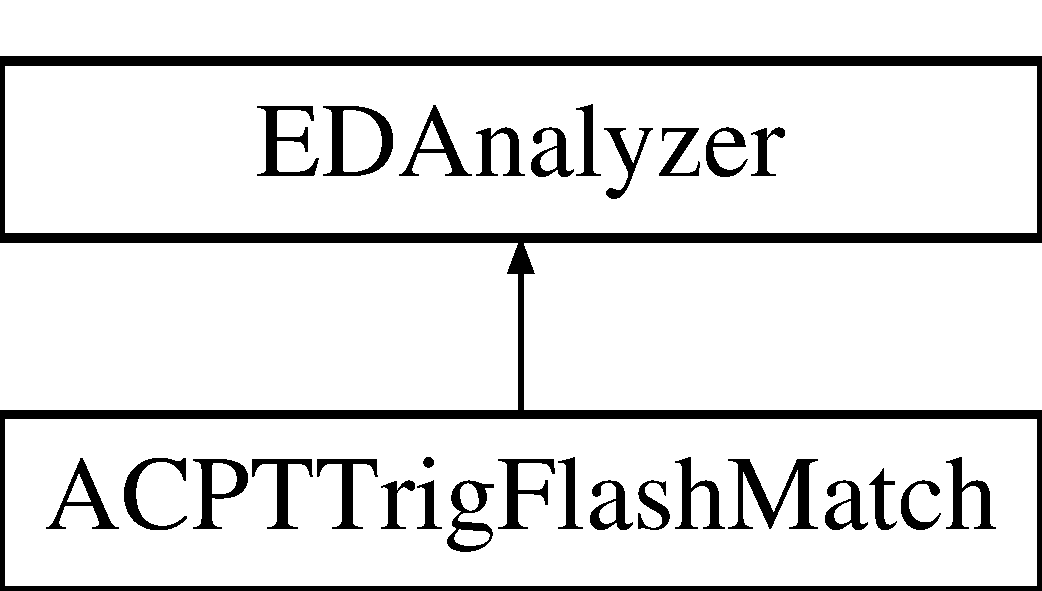
\includegraphics[height=2.000000cm]{classACPTTrigFlashMatch}
\end{center}
\end{figure}
\subsection*{Public Member Functions}
\begin{DoxyCompactItemize}
\item 
\hypertarget{classACPTTrigFlashMatch_a023bad289ce905162bf51061a9ea8a57}{{\bfseries A\-C\-P\-T\-Trig\-Flash\-Match} (fhicl\-::\-Parameter\-Set const \&p)}\label{classACPTTrigFlashMatch_a023bad289ce905162bf51061a9ea8a57}

\item 
\hypertarget{classACPTTrigFlashMatch_a7163ff6a902f715eb65241e9ef29a5d7}{{\bfseries A\-C\-P\-T\-Trig\-Flash\-Match} (\hyperlink{classACPTTrigFlashMatch}{A\-C\-P\-T\-Trig\-Flash\-Match} const \&)=delete}\label{classACPTTrigFlashMatch_a7163ff6a902f715eb65241e9ef29a5d7}

\item 
\hypertarget{classACPTTrigFlashMatch_a4076bcb46f4d41fa115392321797bc9f}{{\bfseries A\-C\-P\-T\-Trig\-Flash\-Match} (\hyperlink{classACPTTrigFlashMatch}{A\-C\-P\-T\-Trig\-Flash\-Match} \&\&)=delete}\label{classACPTTrigFlashMatch_a4076bcb46f4d41fa115392321797bc9f}

\item 
\hypertarget{classACPTTrigFlashMatch_a838017cf67fc68be164910cc77a0cc74}{\hyperlink{classACPTTrigFlashMatch}{A\-C\-P\-T\-Trig\-Flash\-Match} \& {\bfseries operator=} (\hyperlink{classACPTTrigFlashMatch}{A\-C\-P\-T\-Trig\-Flash\-Match} const \&)=delete}\label{classACPTTrigFlashMatch_a838017cf67fc68be164910cc77a0cc74}

\item 
\hypertarget{classACPTTrigFlashMatch_a157f0419b2b3a93cf06551989e694b4d}{\hyperlink{classACPTTrigFlashMatch}{A\-C\-P\-T\-Trig\-Flash\-Match} \& {\bfseries operator=} (\hyperlink{classACPTTrigFlashMatch}{A\-C\-P\-T\-Trig\-Flash\-Match} \&\&)=delete}\label{classACPTTrigFlashMatch_a157f0419b2b3a93cf06551989e694b4d}

\item 
\hypertarget{classACPTTrigFlashMatch_ac752939160dfab34cdd0741a7f715eec}{void {\bfseries analyze} (art\-::\-Event const \&e) override}\label{classACPTTrigFlashMatch_ac752939160dfab34cdd0741a7f715eec}

\item 
\hypertarget{classACPTTrigFlashMatch_ab182358806d46b65d6836573eb4f957d}{void {\bfseries begin\-Job} () override}\label{classACPTTrigFlashMatch_ab182358806d46b65d6836573eb4f957d}

\item 
\hypertarget{classACPTTrigFlashMatch_ae186ed9ccbcbdab43ee65cc856a75c87}{void {\bfseries end\-Job} () override}\label{classACPTTrigFlashMatch_ae186ed9ccbcbdab43ee65cc856a75c87}

\end{DoxyCompactItemize}
\subsection*{Private Attributes}
\begin{DoxyCompactItemize}
\item 
\hypertarget{classACPTTrigFlashMatch_a6c509f7d517ac25379ccf15ffaa5b1af}{T\-Tree $\ast$ {\bfseries \-\_\-tree}}\label{classACPTTrigFlashMatch_a6c509f7d517ac25379ccf15ffaa5b1af}

\item 
\hypertarget{classACPTTrigFlashMatch_adb300d1e540d7b4db814bec89617b4c3}{int {\bfseries \-\_\-run}}\label{classACPTTrigFlashMatch_adb300d1e540d7b4db814bec89617b4c3}

\item 
\hypertarget{classACPTTrigFlashMatch_acdd4472a96aecb7db807fef3d7c0ae3d}{int {\bfseries \-\_\-sub}}\label{classACPTTrigFlashMatch_acdd4472a96aecb7db807fef3d7c0ae3d}

\item 
\hypertarget{classACPTTrigFlashMatch_ac9332a52495a5619b2887dc99fba3b4b}{int {\bfseries \-\_\-evt}}\label{classACPTTrigFlashMatch_ac9332a52495a5619b2887dc99fba3b4b}

\item 
\hypertarget{classACPTTrigFlashMatch_aeb541aeed57710dda186c17d7b526090}{float {\bfseries \-\_\-score}}\label{classACPTTrigFlashMatch_aeb541aeed57710dda186c17d7b526090}

\item 
\hypertarget{classACPTTrigFlashMatch_a595961fecc69b5fdd276c868d415e82d}{int {\bfseries \-\_\-acpt}}\label{classACPTTrigFlashMatch_a595961fecc69b5fdd276c868d415e82d}

\item 
\hypertarget{classACPTTrigFlashMatch_add1a2bd160d71af748c0894f8e04843c}{T\-Tree $\ast$ {\bfseries \-\_\-evt\-\_\-tree}}\label{classACPTTrigFlashMatch_add1a2bd160d71af748c0894f8e04843c}

\item 
\hypertarget{classACPTTrigFlashMatch_a818b0a04513d10606368172e5830a519}{float {\bfseries \-\_\-best\-\_\-score}}\label{classACPTTrigFlashMatch_a818b0a04513d10606368172e5830a519}

\item 
\hypertarget{classACPTTrigFlashMatch_a724e2317a34e6e3bbb9579f51c53cfff}{float {\bfseries \-\_\-acpt\-\_\-score}}\label{classACPTTrigFlashMatch_a724e2317a34e6e3bbb9579f51c53cfff}

\item 
\hypertarget{classACPTTrigFlashMatch_aa278316637008ac1b8cb7beed93c6a3f}{std\-::vector$<$ float $>$ {\bfseries \-\_\-score\-\_\-v}}\label{classACPTTrigFlashMatch_aa278316637008ac1b8cb7beed93c6a3f}

\item 
\hypertarget{classACPTTrigFlashMatch_a020c95be48a14c026eb0dd3bcc27eda0}{int {\bfseries \-\_\-score\-\_\-acpt\-\_\-idx}}\label{classACPTTrigFlashMatch_a020c95be48a14c026eb0dd3bcc27eda0}

\item 
\hypertarget{classACPTTrigFlashMatch_ae62178655c0e2f1fe9ee2b9ac4e9e0bb}{int {\bfseries \-\_\-best\-\_\-acpt}}\label{classACPTTrigFlashMatch_ae62178655c0e2f1fe9ee2b9ac4e9e0bb}

\item 
\hypertarget{classACPTTrigFlashMatch_a4895ce506c834baabf2e4411ff3789ce}{float {\bfseries \-\_\-trk\-\_\-start\-\_\-x}}\label{classACPTTrigFlashMatch_a4895ce506c834baabf2e4411ff3789ce}

\item 
\hypertarget{classACPTTrigFlashMatch_ad6717d4bd82681ec978741ca42edb719}{float {\bfseries \-\_\-trk\-\_\-start\-\_\-y}}\label{classACPTTrigFlashMatch_ad6717d4bd82681ec978741ca42edb719}

\item 
\hypertarget{classACPTTrigFlashMatch_ab27f1b803cfe25365757ff69f941c242}{float {\bfseries \-\_\-trk\-\_\-start\-\_\-z}}\label{classACPTTrigFlashMatch_ab27f1b803cfe25365757ff69f941c242}

\item 
\hypertarget{classACPTTrigFlashMatch_a74b69344ad276bf357cb73812a031c95}{float {\bfseries \-\_\-trk\-\_\-end\-\_\-x}}\label{classACPTTrigFlashMatch_a74b69344ad276bf357cb73812a031c95}

\item 
\hypertarget{classACPTTrigFlashMatch_a8dfbd3ae7035b8a40906bb63a4965167}{float {\bfseries \-\_\-trk\-\_\-end\-\_\-y}}\label{classACPTTrigFlashMatch_a8dfbd3ae7035b8a40906bb63a4965167}

\item 
\hypertarget{classACPTTrigFlashMatch_a0cb660654992d298fa688338aad09c15}{float {\bfseries \-\_\-trk\-\_\-end\-\_\-z}}\label{classACPTTrigFlashMatch_a0cb660654992d298fa688338aad09c15}

\item 
\hypertarget{classACPTTrigFlashMatch_af0770bf40eb0c3ec30fc38f8be779be9}{float {\bfseries \-\_\-trk\-\_\-start\-\_\-x\-\_\-acpt}}\label{classACPTTrigFlashMatch_af0770bf40eb0c3ec30fc38f8be779be9}

\item 
\hypertarget{classACPTTrigFlashMatch_aba48db7fecffcaca8888fd9c9d6af1ae}{float {\bfseries \-\_\-trk\-\_\-start\-\_\-y\-\_\-acpt}}\label{classACPTTrigFlashMatch_aba48db7fecffcaca8888fd9c9d6af1ae}

\item 
\hypertarget{classACPTTrigFlashMatch_a8e0470d01b355799fb774c4c4db62689}{float {\bfseries \-\_\-trk\-\_\-start\-\_\-z\-\_\-acpt}}\label{classACPTTrigFlashMatch_a8e0470d01b355799fb774c4c4db62689}

\item 
\hypertarget{classACPTTrigFlashMatch_a2b626bfbc6a107cc56ae315d6d61d98f}{float {\bfseries \-\_\-trk\-\_\-end\-\_\-x\-\_\-acpt}}\label{classACPTTrigFlashMatch_a2b626bfbc6a107cc56ae315d6d61d98f}

\item 
\hypertarget{classACPTTrigFlashMatch_a18f016888db907d179a9aa3ae6d5845b}{float {\bfseries \-\_\-trk\-\_\-end\-\_\-y\-\_\-acpt}}\label{classACPTTrigFlashMatch_a18f016888db907d179a9aa3ae6d5845b}

\item 
\hypertarget{classACPTTrigFlashMatch_a7b48f6622fa7b3a58a0666c2d5885917}{float {\bfseries \-\_\-trk\-\_\-end\-\_\-z\-\_\-acpt}}\label{classACPTTrigFlashMatch_a7b48f6622fa7b3a58a0666c2d5885917}

\item 
\hypertarget{classACPTTrigFlashMatch_a9c1d4dbb9d83102c10c7f866504d119c}{std\-::vector$<$ float $>$ {\bfseries \-\_\-pe\-Spectrum}}\label{classACPTTrigFlashMatch_a9c1d4dbb9d83102c10c7f866504d119c}

\item 
\hypertarget{classACPTTrigFlashMatch_a2e6924f456d3ddf17ed33c11073f065b}{std\-::vector$<$ float $>$ {\bfseries \-\_\-pe\-Hypothesis}}\label{classACPTTrigFlashMatch_a2e6924f456d3ddf17ed33c11073f065b}

\item 
\hypertarget{classACPTTrigFlashMatch_ae8ff3cf89ddeb66771dbe12166ec723b}{std\-::vector$<$ float $>$ {\bfseries \-\_\-pe\-Spectrum\-\_\-acpt}}\label{classACPTTrigFlashMatch_ae8ff3cf89ddeb66771dbe12166ec723b}

\item 
\hypertarget{classACPTTrigFlashMatch_a029c3101aedd91cbbe5d6422ebf9b676}{std\-::vector$<$ float $>$ {\bfseries \-\_\-pe\-Hypothesis\-\_\-acpt}}\label{classACPTTrigFlashMatch_a029c3101aedd91cbbe5d6422ebf9b676}

\item 
\hypertarget{classACPTTrigFlashMatch_a73c44e19187cb5fcc6a44d1d93c6ceec}{std\-::string {\bfseries f\-P\-F\-Pproducer}}\label{classACPTTrigFlashMatch_a73c44e19187cb5fcc6a44d1d93c6ceec}

\item 
\hypertarget{classACPTTrigFlashMatch_aa487d50e642a754d1fa2130cf6fc4311}{std\-::string {\bfseries f\-Trackproducer}}\label{classACPTTrigFlashMatch_aa487d50e642a754d1fa2130cf6fc4311}

\item 
\hypertarget{classACPTTrigFlashMatch_a37a8ef70c53d0d0e2dd4df71b92ed967}{std\-::string {\bfseries f\-Space\-Pointproducer}}\label{classACPTTrigFlashMatch_a37a8ef70c53d0d0e2dd4df71b92ed967}

\item 
\hypertarget{classACPTTrigFlashMatch_a5c9298a02f961ee72ce941670365c7e7}{std\-::string {\bfseries f\-T0producer}}\label{classACPTTrigFlashMatch_a5c9298a02f961ee72ce941670365c7e7}

\item 
\hypertarget{classACPTTrigFlashMatch_ab870ea0c1f870ff9c2077e466188951e}{bool {\bfseries f\-Only\-Tagged}}\label{classACPTTrigFlashMatch_ab870ea0c1f870ff9c2077e466188951e}

\item 
\hypertarget{classACPTTrigFlashMatch_a12e3a8369411bc0e4608ec08d2cb56c5}{std\-::unique\-\_\-ptr\\*
$<$ \hyperlink{classflashmatch_1_1FlashMatchingToolBase}{flashmatch\-::\-Flash\-Matching\-Tool\-Base} $>$ \hyperlink{classACPTTrigFlashMatch_a12e3a8369411bc0e4608ec08d2cb56c5}{\-\_\-flashmatch\-Tool}}\label{classACPTTrigFlashMatch_a12e3a8369411bc0e4608ec08d2cb56c5}

\begin{DoxyCompactList}\small\item\em The slice id tool. \end{DoxyCompactList}\end{DoxyCompactItemize}


The documentation for this class was generated from the following file\-:\begin{DoxyCompactItemize}
\item 
/home/travis/build/ubneutrinos/searchingfornues/\-Flash\-Matching/A\-C\-P\-T\-Trig\-Flash\-Match\-\_\-module.\-cc\end{DoxyCompactItemize}

\hypertarget{classanalysis_1_1AnalysisToolBase}{}\section{analysis\+:\+:Analysis\+Tool\+Base Class Reference}
\label{classanalysis_1_1AnalysisToolBase}\index{analysis\+::\+Analysis\+Tool\+Base@{analysis\+::\+Analysis\+Tool\+Base}}
Inheritance diagram for analysis\+:\+:Analysis\+Tool\+Base\+:\begin{figure}[H]
\begin{center}
\leavevmode
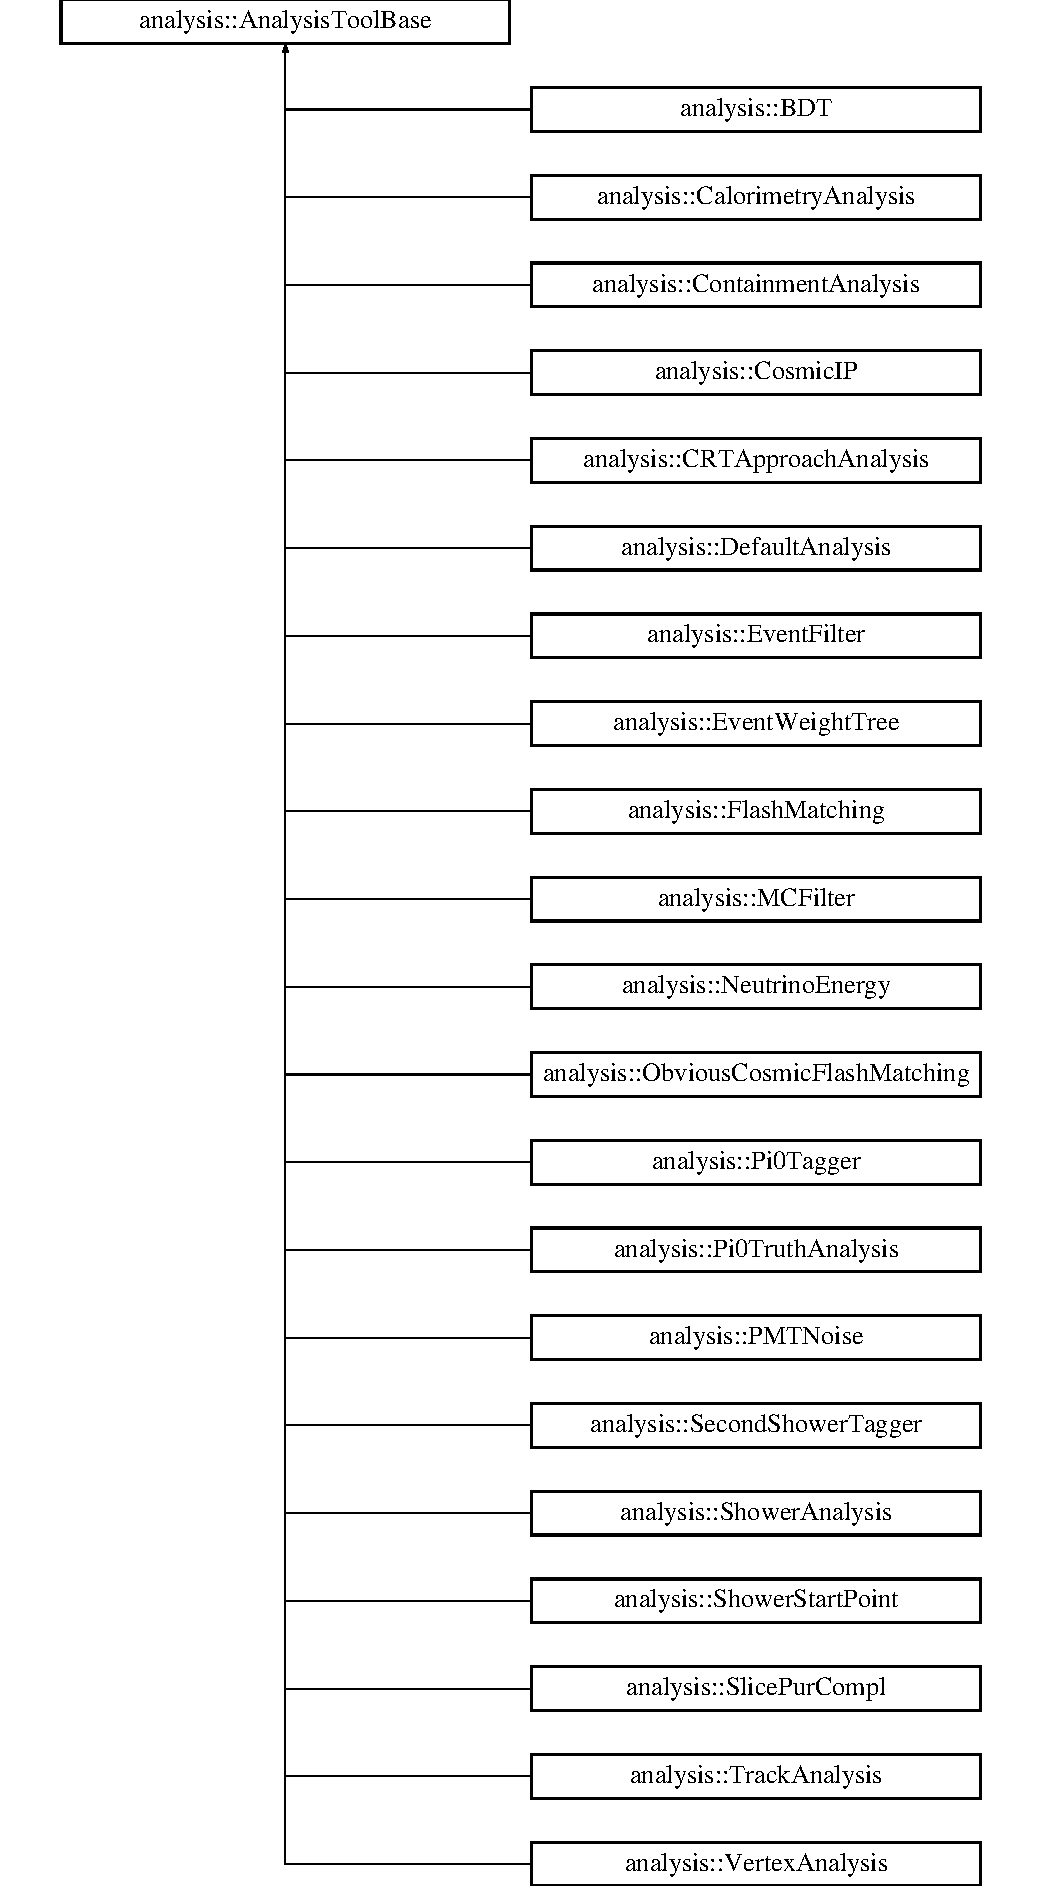
\includegraphics[height=12.000000cm]{classanalysis_1_1AnalysisToolBase}
\end{center}
\end{figure}
\subsection*{Public Member Functions}
\begin{DoxyCompactItemize}
\item 
virtual \hyperlink{classanalysis_1_1AnalysisToolBase_a24a388ad7ccb4007307b2e429acc8967}{$\sim$\+Analysis\+Tool\+Base} () noexcept=default\hypertarget{classanalysis_1_1AnalysisToolBase_a24a388ad7ccb4007307b2e429acc8967}{}\label{classanalysis_1_1AnalysisToolBase_a24a388ad7ccb4007307b2e429acc8967}

\begin{DoxyCompactList}\small\item\em Virtual Destructor. \end{DoxyCompactList}\item 
void \hyperlink{classanalysis_1_1AnalysisToolBase_a99bb8301fb7988663c6febc152e4060f}{configure} (const fhicl\+::\+Parameter\+Set \&)
\begin{DoxyCompactList}\small\item\em Interface for configuring the particular algorithm tool. \end{DoxyCompactList}\item 
virtual void \hyperlink{classanalysis_1_1AnalysisToolBase_ad5079f85c78e6c40f70ebf4ee31f5600}{analyze\+Event} (art\+::\+Event const \&e, bool f\+Data)=0
\begin{DoxyCompactList}\small\item\em Analysis function. \end{DoxyCompactList}\item 
virtual void \hyperlink{classanalysis_1_1AnalysisToolBase_ac1611ea1b1a5db62a6543709ec1d2e96}{analyze\+Slice} (art\+::\+Event const \&e, std\+::vector$<$ Proxy\+Pfp\+Elem\+\_\+t $>$ \&slice\+\_\+pfp\+\_\+v, bool f\+Data, bool selected)=0
\begin{DoxyCompactList}\small\item\em Analysis function. \end{DoxyCompactList}\item 
virtual void \hyperlink{classanalysis_1_1AnalysisToolBase_a03a79460c4d2466d0b9fa102517a4a2d}{set\+Branches} (T\+Tree $\ast$\+\_\+tree)=0\hypertarget{classanalysis_1_1AnalysisToolBase_a03a79460c4d2466d0b9fa102517a4a2d}{}\label{classanalysis_1_1AnalysisToolBase_a03a79460c4d2466d0b9fa102517a4a2d}

\begin{DoxyCompactList}\small\item\em set branches for T\+Tree \end{DoxyCompactList}\item 
virtual void \hyperlink{classanalysis_1_1AnalysisToolBase_a005e4aa5853d1f2ebc4592b73ae3f9cc}{reset\+T\+Tree} (T\+Tree $\ast$\+\_\+tree)=0\hypertarget{classanalysis_1_1AnalysisToolBase_a005e4aa5853d1f2ebc4592b73ae3f9cc}{}\label{classanalysis_1_1AnalysisToolBase_a005e4aa5853d1f2ebc4592b73ae3f9cc}

\begin{DoxyCompactList}\small\item\em resetset T\+Tree branches \end{DoxyCompactList}\end{DoxyCompactItemize}


\subsection{Member Function Documentation}
\index{analysis\+::\+Analysis\+Tool\+Base@{analysis\+::\+Analysis\+Tool\+Base}!analyze\+Event@{analyze\+Event}}
\index{analyze\+Event@{analyze\+Event}!analysis\+::\+Analysis\+Tool\+Base@{analysis\+::\+Analysis\+Tool\+Base}}
\subsubsection[{\texorpdfstring{analyze\+Event(art\+::\+Event const \&e, bool f\+Data)=0}{analyzeEvent(art::Event const &e, bool fData)=0}}]{\setlength{\rightskip}{0pt plus 5cm}virtual void analysis\+::\+Analysis\+Tool\+Base\+::analyze\+Event (
\begin{DoxyParamCaption}
\item[{art\+::\+Event const \&}]{e, }
\item[{bool}]{f\+Data}
\end{DoxyParamCaption}
)\hspace{0.3cm}{\ttfamily [pure virtual]}}\hypertarget{classanalysis_1_1AnalysisToolBase_ad5079f85c78e6c40f70ebf4ee31f5600}{}\label{classanalysis_1_1AnalysisToolBase_ad5079f85c78e6c40f70ebf4ee31f5600}


Analysis function. 


\begin{DoxyParams}{Parameters}
{\em art\+::\+Event} & event record for analysis \\
\hline
\end{DoxyParams}


Implemented in \hyperlink{classanalysis_1_1CRTApproachAnalysis_ad367db2555c9f7b34b9854e3e21bf9ca}{analysis\+::\+C\+R\+T\+Approach\+Analysis}, \hyperlink{classanalysis_1_1ObviousCosmicFlashMatching_ac2abf5075cbd03ffde102e14ae260707}{analysis\+::\+Obvious\+Cosmic\+Flash\+Matching}, \hyperlink{classanalysis_1_1PMTNoise_a939447b8cffa89d11d7f7bc3c99378a6}{analysis\+::\+P\+M\+T\+Noise}, \hyperlink{classanalysis_1_1TrackAnalysis_aa5a295fc3fe8aa050905361f469ff108}{analysis\+::\+Track\+Analysis}, \hyperlink{classanalysis_1_1CosmicIP_aece9b4c45c6e1771df582b2c5e40c5d5}{analysis\+::\+Cosmic\+IP}, \hyperlink{classanalysis_1_1FlashMatching_ab3bc034486cadaeda1c4c0868a7f17f1}{analysis\+::\+Flash\+Matching}, \hyperlink{classanalysis_1_1DefaultAnalysis_a0cf6d593602ba67c23fae67ca7989c10}{analysis\+::\+Default\+Analysis}, \hyperlink{classanalysis_1_1Pi0TruthAnalysis_a07cf437c5f9d2b19b7a0ca3de447d12f}{analysis\+::\+Pi0\+Truth\+Analysis}, \hyperlink{classanalysis_1_1ShowerAnalysis_a5ae15109590ea737320bf13cefa5cc3f}{analysis\+::\+Shower\+Analysis}, \hyperlink{classanalysis_1_1ContainmentAnalysis_a5bcf033310f0e8f58fd6f4f46f216985}{analysis\+::\+Containment\+Analysis}, \hyperlink{classanalysis_1_1SlicePurCompl_af71528c37c501d30f5bbc1e75b50b3f6}{analysis\+::\+Slice\+Pur\+Compl}, \hyperlink{classanalysis_1_1BDT_abadae5b35cecaca0409c0ba659aa7b82}{analysis\+::\+B\+DT}, and \hyperlink{classanalysis_1_1EventWeightTree_a1af84126be9ecd2ae71013db4d2c1af7}{analysis\+::\+Event\+Weight\+Tree}.

\index{analysis\+::\+Analysis\+Tool\+Base@{analysis\+::\+Analysis\+Tool\+Base}!analyze\+Slice@{analyze\+Slice}}
\index{analyze\+Slice@{analyze\+Slice}!analysis\+::\+Analysis\+Tool\+Base@{analysis\+::\+Analysis\+Tool\+Base}}
\subsubsection[{\texorpdfstring{analyze\+Slice(art\+::\+Event const \&e, std\+::vector$<$ Proxy\+Pfp\+Elem\+\_\+t $>$ \&slice\+\_\+pfp\+\_\+v, bool f\+Data, bool selected)=0}{analyzeSlice(art::Event const &e, std::vector< ProxyPfpElem_t > &slice_pfp_v, bool fData, bool selected)=0}}]{\setlength{\rightskip}{0pt plus 5cm}virtual void analysis\+::\+Analysis\+Tool\+Base\+::analyze\+Slice (
\begin{DoxyParamCaption}
\item[{art\+::\+Event const \&}]{e, }
\item[{std\+::vector$<$ Proxy\+Pfp\+Elem\+\_\+t $>$ \&}]{slice\+\_\+pfp\+\_\+v, }
\item[{bool}]{f\+Data, }
\item[{bool}]{selected}
\end{DoxyParamCaption}
)\hspace{0.3cm}{\ttfamily [pure virtual]}}\hypertarget{classanalysis_1_1AnalysisToolBase_ac1611ea1b1a5db62a6543709ec1d2e96}{}\label{classanalysis_1_1AnalysisToolBase_ac1611ea1b1a5db62a6543709ec1d2e96}


Analysis function. 


\begin{DoxyParams}{Parameters}
{\em art\+::\+Event} & event record for analysis \\
\hline
\end{DoxyParams}


Implemented in \hyperlink{classanalysis_1_1CRTApproachAnalysis_a1ec2e53aa488645ad8c7ba625699d394}{analysis\+::\+C\+R\+T\+Approach\+Analysis}, \hyperlink{classanalysis_1_1ObviousCosmicFlashMatching_adbdb066be56f971dc6dc4191a56b5693}{analysis\+::\+Obvious\+Cosmic\+Flash\+Matching}, \hyperlink{classanalysis_1_1PMTNoise_a4c427fe82fe00639048c4a04e29155c8}{analysis\+::\+P\+M\+T\+Noise}, \hyperlink{classanalysis_1_1TrackAnalysis_a00e51059eed5a6486c9eb2f2f16017de}{analysis\+::\+Track\+Analysis}, \hyperlink{classanalysis_1_1CosmicIP_a86c9683c997d233949d8116940918e32}{analysis\+::\+Cosmic\+IP}, \hyperlink{classanalysis_1_1FlashMatching_acdff3053951979de66145a37a41f1767}{analysis\+::\+Flash\+Matching}, \hyperlink{classanalysis_1_1DefaultAnalysis_ad676faeeb49900efb0c9a615a60d179c}{analysis\+::\+Default\+Analysis}, \hyperlink{classanalysis_1_1Pi0TruthAnalysis_a02b3f2e32b0e8097c0432bd013c0dbe1}{analysis\+::\+Pi0\+Truth\+Analysis}, \hyperlink{classanalysis_1_1ShowerAnalysis_a957be06c08e5777cd684c84ca53bc45e}{analysis\+::\+Shower\+Analysis}, \hyperlink{classanalysis_1_1ContainmentAnalysis_a6e3c839d18ff3001b46be5fde80a5d04}{analysis\+::\+Containment\+Analysis}, \hyperlink{classanalysis_1_1SlicePurCompl_ab13316464f9ed61e81b18d59ca38d9a1}{analysis\+::\+Slice\+Pur\+Compl}, \hyperlink{classanalysis_1_1BDT_ab31b4dac24b518a017d4a1898c76991d}{analysis\+::\+B\+DT}, and \hyperlink{classanalysis_1_1EventWeightTree_a2e30de7f19d6f20e6c3f7ffdb41b22a6}{analysis\+::\+Event\+Weight\+Tree}.

\index{analysis\+::\+Analysis\+Tool\+Base@{analysis\+::\+Analysis\+Tool\+Base}!configure@{configure}}
\index{configure@{configure}!analysis\+::\+Analysis\+Tool\+Base@{analysis\+::\+Analysis\+Tool\+Base}}
\subsubsection[{\texorpdfstring{configure(const fhicl\+::\+Parameter\+Set \&)}{configure(const fhicl::ParameterSet &)}}]{\setlength{\rightskip}{0pt plus 5cm}void analysis\+::\+Analysis\+Tool\+Base\+::configure (
\begin{DoxyParamCaption}
\item[{const fhicl\+::\+Parameter\+Set \&}]{}
\end{DoxyParamCaption}
)\hspace{0.3cm}{\ttfamily [inline]}}\hypertarget{classanalysis_1_1AnalysisToolBase_a99bb8301fb7988663c6febc152e4060f}{}\label{classanalysis_1_1AnalysisToolBase_a99bb8301fb7988663c6febc152e4060f}


Interface for configuring the particular algorithm tool. 


\begin{DoxyParams}{Parameters}
{\em Parameter\+Set} & The input set of parameters for configuration \\
\hline
\end{DoxyParams}


The documentation for this class was generated from the following file\+:\begin{DoxyCompactItemize}
\item 
/home/travis/build/ubneutrinos/searchingfornues/\+Selection/\+Analysis\+Tools/Analysis\+Tool\+Base.\+h\end{DoxyCompactItemize}

\hypertarget{structsearchingfornues_1_1BtPart}{\section{searchingfornues\-:\-:Bt\-Part Struct Reference}
\label{structsearchingfornues_1_1BtPart}\index{searchingfornues\-::\-Bt\-Part@{searchingfornues\-::\-Bt\-Part}}
}
\subsection*{Public Member Functions}
\begin{DoxyCompactItemize}
\item 
\hypertarget{structsearchingfornues_1_1BtPart_a00003f0908892d8a64f80a8b3f2e6f90}{{\bfseries Bt\-Part} (const int pdg\-\_\-, const float px\-\_\-, const float py\-\_\-, const float pz\-\_\-, const float e\-\_\-, const std\-::vector$<$ unsigned int $>$ \&tids\-\_\-)}\label{structsearchingfornues_1_1BtPart_a00003f0908892d8a64f80a8b3f2e6f90}

\item 
\hypertarget{structsearchingfornues_1_1BtPart_a69048423846c19666791da82138ce613}{{\bfseries Bt\-Part} (const int pdg\-\_\-, const float px\-\_\-, const float py\-\_\-, const float pz\-\_\-, const float e\-\_\-, const unsigned int tid\-\_\-)}\label{structsearchingfornues_1_1BtPart_a69048423846c19666791da82138ce613}

\end{DoxyCompactItemize}
\subsection*{Public Attributes}
\begin{DoxyCompactItemize}
\item 
\hypertarget{structsearchingfornues_1_1BtPart_a4adfa8d6e2aab316bfda7d64d6cecb3e}{int {\bfseries pdg}}\label{structsearchingfornues_1_1BtPart_a4adfa8d6e2aab316bfda7d64d6cecb3e}

\item 
\hypertarget{structsearchingfornues_1_1BtPart_a3a0ddc2493391fd58b384792e0a1a5fd}{float {\bfseries px}}\label{structsearchingfornues_1_1BtPart_a3a0ddc2493391fd58b384792e0a1a5fd}

\item 
\hypertarget{structsearchingfornues_1_1BtPart_a7862a99921a6cdc435f401c4a7c70668}{float {\bfseries py}}\label{structsearchingfornues_1_1BtPart_a7862a99921a6cdc435f401c4a7c70668}

\item 
\hypertarget{structsearchingfornues_1_1BtPart_ad65a32274c4b8b61a78739ed76080f3b}{float {\bfseries pz}}\label{structsearchingfornues_1_1BtPart_ad65a32274c4b8b61a78739ed76080f3b}

\item 
\hypertarget{structsearchingfornues_1_1BtPart_a0037317972c950fac8188464838a9645}{float {\bfseries e}}\label{structsearchingfornues_1_1BtPart_a0037317972c950fac8188464838a9645}

\item 
\hypertarget{structsearchingfornues_1_1BtPart_a0584d6c3edff2a6483d1fa94fd2d7a8c}{std\-::vector$<$ unsigned int $>$ {\bfseries tids}}\label{structsearchingfornues_1_1BtPart_a0584d6c3edff2a6483d1fa94fd2d7a8c}

\item 
\hypertarget{structsearchingfornues_1_1BtPart_a053f98b42289602fdeb9ca36e63fe0ee}{int {\bfseries nhits} = 0}\label{structsearchingfornues_1_1BtPart_a053f98b42289602fdeb9ca36e63fe0ee}

\end{DoxyCompactItemize}


The documentation for this struct was generated from the following file\-:\begin{DoxyCompactItemize}
\item 
/home/travis/build/ubneutrinos/searchingfornues/\-Selection/\-Common\-Defs/Backtracking\-Funcs.\-h\end{DoxyCompactItemize}

\hypertarget{classselection_1_1CC0piNpSelection}{}\section{selection\+:\+:C\+C0pi\+Np\+Selection Class Reference}
\label{classselection_1_1CC0piNpSelection}\index{selection\+::\+C\+C0pi\+Np\+Selection@{selection\+::\+C\+C0pi\+Np\+Selection}}
Inheritance diagram for selection\+:\+:C\+C0pi\+Np\+Selection\+:\begin{figure}[H]
\begin{center}
\leavevmode
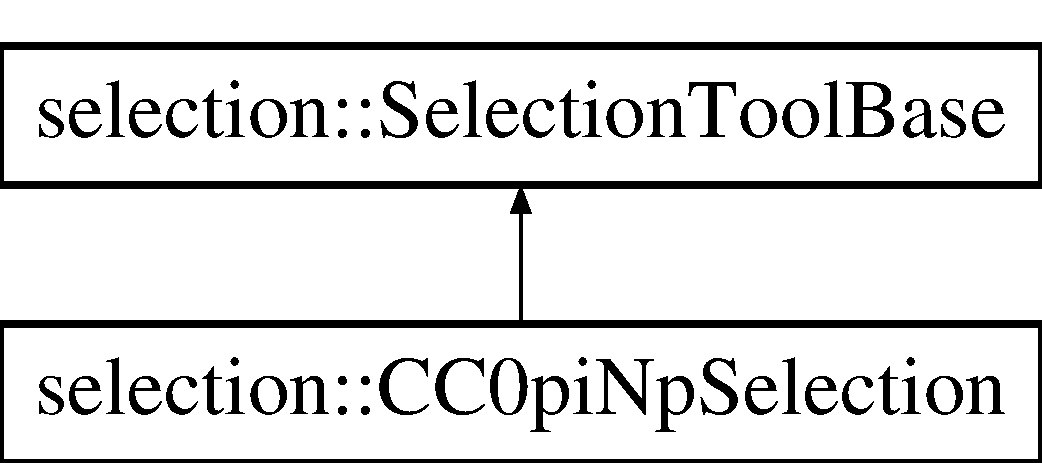
\includegraphics[height=2.000000cm]{classselection_1_1CC0piNpSelection}
\end{center}
\end{figure}
\subsection*{Public Member Functions}
\begin{DoxyCompactItemize}
\item 
\hyperlink{classselection_1_1CC0piNpSelection_a5770519e6639db45cb9f3a4b1bf3efc2}{C\+C0pi\+Np\+Selection} (const fhicl\+::\+Parameter\+Set \&pset)
\begin{DoxyCompactList}\small\item\em Constructor. \end{DoxyCompactList}\item 
\hyperlink{classselection_1_1CC0piNpSelection_a7f809f358e84885ae2f08f54b4b8183b}{$\sim$\+C\+C0pi\+Np\+Selection} ()\hypertarget{classselection_1_1CC0piNpSelection_a7f809f358e84885ae2f08f54b4b8183b}{}\label{classselection_1_1CC0piNpSelection_a7f809f358e84885ae2f08f54b4b8183b}

\begin{DoxyCompactList}\small\item\em Destructor. \end{DoxyCompactList}\item 
void \hyperlink{classselection_1_1CC0piNpSelection_ace78372ffb6d92911f79ded647aacf4c}{configure} (fhicl\+::\+Parameter\+Set const \&pset)
\item 
bool \hyperlink{classselection_1_1CC0piNpSelection_aee88d296a2ebad59acadfd919139d96f}{select\+Event} (art\+::\+Event const \&e, const std\+::vector$<$ Proxy\+Pfp\+Elem\+\_\+t $>$ \&pfp\+\_\+pxy\+\_\+v)
\begin{DoxyCompactList}\small\item\em Selection function. \end{DoxyCompactList}\item 
void \hyperlink{classselection_1_1CC0piNpSelection_a6a14e4d0ff713ed2c75055019d278422}{set\+Branches} (T\+Tree $\ast$\+\_\+tree)
\begin{DoxyCompactList}\small\item\em Set branches for T\+Tree. \end{DoxyCompactList}\item 
void \hyperlink{classselection_1_1CC0piNpSelection_a3d7a6aa0fbd41f4a77390a160ee64e35}{reset\+T\+Tree} (T\+Tree $\ast$\+\_\+tree)
\begin{DoxyCompactList}\small\item\em Reset T\+Tree branches. \end{DoxyCompactList}\end{DoxyCompactItemize}
\subsection*{Private Attributes}
\begin{DoxyCompactItemize}
\item 
const trkf\+::\+Track\+Momentum\+Calculator {\bfseries \+\_\+trkmom}\hypertarget{classselection_1_1CC0piNpSelection_a320b14dcb3cc1674048bc4f0dd18fa45}{}\label{classselection_1_1CC0piNpSelection_a320b14dcb3cc1674048bc4f0dd18fa45}

\item 
const trkf\+::\+Trajectory\+M\+C\+S\+Fitter {\bfseries mcsfitter}\hypertarget{classselection_1_1CC0piNpSelection_aab7c56654d30a9cc5ad2dbe09a3e12c9}{}\label{classselection_1_1CC0piNpSelection_aab7c56654d30a9cc5ad2dbe09a3e12c9}

\item 
T\+Particle\+P\+DG $\ast$ {\bfseries proton} = T\+Database\+P\+D\+G\+::\+Instance()-\/$>$Get\+Particle(2212)\hypertarget{classselection_1_1CC0piNpSelection_a721706e2b68efe51225fa6388bc184d1}{}\label{classselection_1_1CC0piNpSelection_a721706e2b68efe51225fa6388bc184d1}

\item 
T\+Particle\+P\+DG $\ast$ {\bfseries electron} = T\+Database\+P\+D\+G\+::\+Instance()-\/$>$Get\+Particle(11)\hypertarget{classselection_1_1CC0piNpSelection_ad04f8899cec1c9c54e720126e61a872f}{}\label{classselection_1_1CC0piNpSelection_ad04f8899cec1c9c54e720126e61a872f}

\item 
T\+Particle\+P\+DG $\ast$ {\bfseries muon} = T\+Database\+P\+D\+G\+::\+Instance()-\/$>$Get\+Particle(13)\hypertarget{classselection_1_1CC0piNpSelection_ae1161170f7b46e368ad608924cc412fd}{}\label{classselection_1_1CC0piNpSelection_ae1161170f7b46e368ad608924cc412fd}

\item 
T\+Particle\+P\+DG $\ast$ {\bfseries pion} = T\+Database\+P\+D\+G\+::\+Instance()-\/$>$Get\+Particle(211)\hypertarget{classselection_1_1CC0piNpSelection_a7237863b296cd8e3bf68dccb4d4122bb}{}\label{classselection_1_1CC0piNpSelection_a7237863b296cd8e3bf68dccb4d4122bb}

\item 
T\+Particle\+P\+DG $\ast$ {\bfseries kaon} = T\+Database\+P\+D\+G\+::\+Instance()-\/$>$Get\+Particle(321)\hypertarget{classselection_1_1CC0piNpSelection_a1881dd29c46973578cb8b48a726f34f0}{}\label{classselection_1_1CC0piNpSelection_a1881dd29c46973578cb8b48a726f34f0}

\item 
float \hyperlink{classselection_1_1CC0piNpSelection_ab72eccf7dab3acafa294a0d8f3e225a0}{f\+Trk\+Shrscore}
\item 
float \hyperlink{classselection_1_1CC0piNpSelection_afe5a2b82ecad103b98362839094c47e0}{f\+Fidvol\+Zstart}
\item 
float \hyperlink{classselection_1_1CC0piNpSelection_a9ac28bcb4ef95573d416dec35202b18e}{f\+Fidvol\+Zend}
\item 
float \hyperlink{classselection_1_1CC0piNpSelection_ac59a66f695af8314018029e4480db16a}{f\+Fidvol\+Ystart}
\item 
float \hyperlink{classselection_1_1CC0piNpSelection_a4732dc1091cb1881c741d57f999b5035}{f\+Fidvol\+Yend}
\item 
float \hyperlink{classselection_1_1CC0piNpSelection_a783e7f9dcd42c083658870f7d23931da}{f\+Fidvol\+Xstart}
\item 
float \hyperlink{classselection_1_1CC0piNpSelection_a754589459e1f2d90a8ad853c68f864db}{f\+Fidvol\+Xend}
\item 
float {\bfseries fd\+Edxcm\+Skip}\hypertarget{classselection_1_1CC0piNpSelection_ac1f5c52f574f9a6f2a45ee3e26340cb0}{}\label{classselection_1_1CC0piNpSelection_ac1f5c52f574f9a6f2a45ee3e26340cb0}

\item 
float {\bfseries fd\+Edxcm\+Len}\hypertarget{classselection_1_1CC0piNpSelection_af2df6516832e3db51a99f7a511a8ad3c}{}\label{classselection_1_1CC0piNpSelection_af2df6516832e3db51a99f7a511a8ad3c}

\item 
bool {\bfseries f\+Save\+More\+Dedx}\hypertarget{classselection_1_1CC0piNpSelection_ac6b2c89b1bd8219eec94ed07c6d47a23}{}\label{classselection_1_1CC0piNpSelection_ac6b2c89b1bd8219eec94ed07c6d47a23}

\item 
bool {\bfseries f\+Locald\+Edx}\hypertarget{classselection_1_1CC0piNpSelection_a62ba49011db390411711289eef29e98a}{}\label{classselection_1_1CC0piNpSelection_a62ba49011db390411711289eef29e98a}

\item 
std\+::vector$<$ float $>$ {\bfseries f\+A\+D\+CtoE}\hypertarget{classselection_1_1CC0piNpSelection_a3d0e422f46814dcd6bd66a8991e11fa9}{}\label{classselection_1_1CC0piNpSelection_a3d0e422f46814dcd6bd66a8991e11fa9}

\item 
bool {\bfseries f\+Recalibrate\+Hits}\hypertarget{classselection_1_1CC0piNpSelection_aa18a4cbc7a9b902c7bfb38ef03ea3f78}{}\label{classselection_1_1CC0piNpSelection_aa18a4cbc7a9b902c7bfb38ef03ea3f78}

\item 
float {\bfseries f\+Energy\+Threshold\+For\+M\+C\+Hits}\hypertarget{classselection_1_1CC0piNpSelection_a99895d76eae50c765fa1ac046d4bdedc}{}\label{classselection_1_1CC0piNpSelection_a99895d76eae50c765fa1ac046d4bdedc}

\item 
\hyperlink{classsearchingfornues_1_1LLRPID}{searchingfornues\+::\+L\+L\+R\+P\+ID} {\bfseries llr\+\_\+pid\+\_\+calculator\+\_\+shr}\hypertarget{classselection_1_1CC0piNpSelection_a9810f1a43b16f39021a80978df9682b7}{}\label{classselection_1_1CC0piNpSelection_a9810f1a43b16f39021a80978df9682b7}

\item 
\hyperlink{structsearchingfornues_1_1ElectronPhotonLookUpParameters}{searchingfornues\+::\+Electron\+Photon\+Look\+Up\+Parameters} {\bfseries electronphoton\+\_\+parameters}\hypertarget{classselection_1_1CC0piNpSelection_ad9e23a1e0f7318e83e1904bc0e377524}{}\label{classselection_1_1CC0piNpSelection_ad9e23a1e0f7318e83e1904bc0e377524}

\item 
\hyperlink{structsearchingfornues_1_1CorrectionLookUpParameters}{searchingfornues\+::\+Correction\+Look\+Up\+Parameters} {\bfseries correction\+\_\+parameters}\hypertarget{classselection_1_1CC0piNpSelection_a3f2b5ec710659b4a382ed3e74e5a671e}{}\label{classselection_1_1CC0piNpSelection_a3f2b5ec710659b4a382ed3e74e5a671e}

\item 
art\+::\+Input\+Tag {\bfseries f\+C\+L\+Sproducer}\hypertarget{classselection_1_1CC0piNpSelection_a3d64505ea3757aa3d729aca8e871cd95}{}\label{classselection_1_1CC0piNpSelection_a3d64505ea3757aa3d729aca8e871cd95}

\item 
art\+::\+Input\+Tag {\bfseries f\+P\+I\+Dproducer}\hypertarget{classselection_1_1CC0piNpSelection_a84fa0549ef1d05cdcbc93b8ab7f6613e}{}\label{classselection_1_1CC0piNpSelection_a84fa0549ef1d05cdcbc93b8ab7f6613e}

\item 
art\+::\+Input\+Tag {\bfseries f\+T\+R\+Kproducer}\hypertarget{classselection_1_1CC0piNpSelection_ac196a716edaba0c3fcc8f20c4ac1af61}{}\label{classselection_1_1CC0piNpSelection_ac196a716edaba0c3fcc8f20c4ac1af61}

\item 
art\+::\+Input\+Tag {\bfseries f\+T\+R\+Kproducer\+Trk\+Fit}\hypertarget{classselection_1_1CC0piNpSelection_a2a418cbcd9bdd0dc488a52af9d588abf}{}\label{classselection_1_1CC0piNpSelection_a2a418cbcd9bdd0dc488a52af9d588abf}

\item 
art\+::\+Input\+Tag {\bfseries f\+Backtrack\+Tag}\hypertarget{classselection_1_1CC0piNpSelection_a43105132eeb5927fb745f1c831915a1b}{}\label{classselection_1_1CC0piNpSelection_a43105132eeb5927fb745f1c831915a1b}

\item 
art\+::\+Input\+Tag {\bfseries f\+Hproducer}\hypertarget{classselection_1_1CC0piNpSelection_a7142f01060887fdaf91e2a44edae8c6f}{}\label{classselection_1_1CC0piNpSelection_a7142f01060887fdaf91e2a44edae8c6f}

\item 
art\+::\+Input\+Tag {\bfseries f\+M\+C\+Rproducer}\hypertarget{classselection_1_1CC0piNpSelection_a2512859a8ce467998cfae65268d01003}{}\label{classselection_1_1CC0piNpSelection_a2512859a8ce467998cfae65268d01003}

\item 
art\+::\+Input\+Tag {\bfseries f\+M\+C\+Pproducer}\hypertarget{classselection_1_1CC0piNpSelection_a97505974a12ecb05ae7888f4647bde1f}{}\label{classselection_1_1CC0piNpSelection_a97505974a12ecb05ae7888f4647bde1f}

\item 
art\+::\+Input\+Tag {\bfseries f\+C\+A\+Lproducer}\hypertarget{classselection_1_1CC0piNpSelection_a5f6c345d0e3a50660957b2787a520a22}{}\label{classselection_1_1CC0piNpSelection_a5f6c345d0e3a50660957b2787a520a22}

\item 
art\+::\+Input\+Tag {\bfseries f\+C\+A\+Lproducer\+Trk\+Fit}\hypertarget{classselection_1_1CC0piNpSelection_af4b580a7c372a5e42b268618a320d600}{}\label{classselection_1_1CC0piNpSelection_af4b580a7c372a5e42b268618a320d600}

\item 
art\+::\+Input\+Tag {\bfseries f\+Clusterproducer}\hypertarget{classselection_1_1CC0piNpSelection_a65d23808ef7623c10076a263fe3f104c}{}\label{classselection_1_1CC0piNpSelection_a65d23808ef7623c10076a263fe3f104c}

\item 
art\+::\+Input\+Tag {\bfseries f\+Hitproducer}\hypertarget{classselection_1_1CC0piNpSelection_ad47ab57ebe8de8ad701d34279ff7f6e4}{}\label{classselection_1_1CC0piNpSelection_ad47ab57ebe8de8ad701d34279ff7f6e4}

\item 
float {\bfseries \+\_\+wire2cm}\hypertarget{classselection_1_1CC0piNpSelection_a07f72f946488ee47d99be315e699ba63}{}\label{classselection_1_1CC0piNpSelection_a07f72f946488ee47d99be315e699ba63}

\item 
float {\bfseries \+\_\+time2cm}\hypertarget{classselection_1_1CC0piNpSelection_a558b5565d41a4c34a61880faf7ffcf94}{}\label{classselection_1_1CC0piNpSelection_a558b5565d41a4c34a61880faf7ffcf94}

\item 
unsigned int \hyperlink{classselection_1_1CC0piNpSelection_aebf4a69b8d7f3171ad90c382668c22ec}{\+\_\+n\+\_\+showers\+\_\+contained}
\item 
unsigned int \hyperlink{classselection_1_1CC0piNpSelection_a22c5cd4cf8882fa3cbabf25ed86d1f39}{\+\_\+n\+\_\+tracks\+\_\+contained}
\item 
unsigned int \hyperlink{classselection_1_1CC0piNpSelection_a750834ef52299d85f9596bbbafa1dffb}{\+\_\+shr\+\_\+hits\+\_\+max}
\item 
unsigned int \hyperlink{classselection_1_1CC0piNpSelection_a247d186cb641d28f8ea5b02c4f2a39bc}{\+\_\+trk\+\_\+hits\+\_\+max}
\item 
unsigned int \hyperlink{classselection_1_1CC0piNpSelection_aa6e7162371e3e343df001f0afc8a20b8}{\+\_\+shr\+\_\+hits\+\_\+tot}
\item 
unsigned int \hyperlink{classselection_1_1CC0piNpSelection_a420b9962478d7998282e03f1ccf89c2e}{\+\_\+trk\+\_\+hits\+\_\+tot}
\item 
unsigned int \hyperlink{classselection_1_1CC0piNpSelection_a76eb07fcb9190709464880c0ea7c4eba}{\+\_\+trk\+\_\+hits\+\_\+y\+\_\+tot}
\item 
unsigned int \hyperlink{classselection_1_1CC0piNpSelection_a30fe5ccb6a299f7955125aa6c9d5923d}{\+\_\+trk\+\_\+hits\+\_\+v\+\_\+tot}
\item 
unsigned int \hyperlink{classselection_1_1CC0piNpSelection_af7d0e867df8901ff3e531b4c1b96408a}{\+\_\+trk\+\_\+hits\+\_\+u\+\_\+tot}
\item 
unsigned int \hyperlink{classselection_1_1CC0piNpSelection_a6a43c3523af47860ad1682ebe14bb8e3}{\+\_\+shr\+\_\+hits\+\_\+y\+\_\+tot}
\item 
unsigned int \hyperlink{classselection_1_1CC0piNpSelection_ab6aaf4282fa9d2e5971e162c66901227}{\+\_\+shr\+\_\+hits\+\_\+v\+\_\+tot}
\item 
unsigned int \hyperlink{classselection_1_1CC0piNpSelection_afba4a31f84c2f125323b90f007bda1c6}{\+\_\+shr\+\_\+hits\+\_\+u\+\_\+tot}
\item 
float \hyperlink{classselection_1_1CC0piNpSelection_abf854f061d0476dc08ae8b3d71e7a86d}{\+\_\+shr\+\_\+energy}
\item 
float \hyperlink{classselection_1_1CC0piNpSelection_a6e42f011e79f646f36df7148907d1b59}{\+\_\+shr\+\_\+energy\+\_\+tot}
\item 
float \hyperlink{classselection_1_1CC0piNpSelection_a910f18dc66ac2f22aa8cbdd6b86c7d0e}{\+\_\+shr\+\_\+energy\+\_\+cali}
\item 
float \hyperlink{classselection_1_1CC0piNpSelection_aae69f88600d31bb3456808268fb63c1c}{\+\_\+shr\+\_\+energy\+\_\+tot\+\_\+cali}
\item 
float \hyperlink{classselection_1_1CC0piNpSelection_a1af96c31bd3afe4b111f429927bbff1c}{\+\_\+shr\+\_\+dedx\+\_\+Y}
\item 
float \hyperlink{classselection_1_1CC0piNpSelection_a392211f6d023d92bf113c20098c5e7fe}{\+\_\+shr\+\_\+dedx\+\_\+V}
\item 
float \hyperlink{classselection_1_1CC0piNpSelection_ada2f72c2f814e7d06c24a50ff5ad4fcc}{\+\_\+shr\+\_\+dedx\+\_\+U}
\item 
float \hyperlink{classselection_1_1CC0piNpSelection_a114f4276a8931d33d8f77fede58398fa}{\+\_\+shr\+\_\+dedx\+\_\+\+Y\+\_\+cali}
\item 
float \hyperlink{classselection_1_1CC0piNpSelection_a0ef852fb0ecd8a3b6f871ed765be12da}{\+\_\+shr\+\_\+dedx\+\_\+\+V\+\_\+cali}
\item 
float \hyperlink{classselection_1_1CC0piNpSelection_a7c90820db5398c179aef3186ab11e521}{\+\_\+shr\+\_\+dedx\+\_\+\+U\+\_\+cali}
\item 
float \hyperlink{classselection_1_1CC0piNpSelection_a20705dc212e16009a0ce4ace27d54af7}{\+\_\+shr\+\_\+distance}
\item 
float \hyperlink{classselection_1_1CC0piNpSelection_a73d772bb569336b56a3f14cee752e2f3}{\+\_\+tksh\+\_\+distance}
\item 
float \hyperlink{classselection_1_1CC0piNpSelection_a959adc6093ff4d2730dac8f75dd1245c}{\+\_\+tksh\+\_\+angle}
\item 
float \hyperlink{classselection_1_1CC0piNpSelection_a8210028b7144d3dc078201257a1a8663}{\+\_\+tksh\+\_\+angle\+\_\+muon}
\item 
float \hyperlink{classselection_1_1CC0piNpSelection_a9033ad097ef1b7a4e10b2b872b82f068}{\+\_\+shr\+\_\+score}
\item 
float \hyperlink{classselection_1_1CC0piNpSelection_a624a38f7c8d33320df92e610fd0e16ee}{\+\_\+shr\+\_\+theta}
\item 
float \hyperlink{classselection_1_1CC0piNpSelection_a8706a83b3dc2e2c3857ada556392f16f}{\+\_\+shr\+\_\+phi}
\item 
float \hyperlink{classselection_1_1CC0piNpSelection_a52e2043c82f5de7f93ac9bad63563f18}{\+\_\+shr\+\_\+px}
\item 
float \hyperlink{classselection_1_1CC0piNpSelection_a436dd7081c84003dabb595289d745111}{\+\_\+shr\+\_\+py}
\item 
float \hyperlink{classselection_1_1CC0piNpSelection_a769319ad32b6ce49c7a5283b246303fa}{\+\_\+shr\+\_\+pz}
\item 
float \hyperlink{classselection_1_1CC0piNpSelection_a47b08d4ae98f51032f431873321914a5}{\+\_\+shr\+\_\+pca\+\_\+0}
\item 
float \hyperlink{classselection_1_1CC0piNpSelection_ae3ce85b9e7002cfac57e433ee131868d}{\+\_\+shr\+\_\+pca\+\_\+1}
\item 
float \hyperlink{classselection_1_1CC0piNpSelection_a7e5a1ac6cd32eec7da00eb45c49df0cd}{\+\_\+shr\+\_\+pca\+\_\+2}
\item 
float \hyperlink{classselection_1_1CC0piNpSelection_a33b26acb3cdb05cb1b81800d8af48a03}{\+\_\+shr\+\_\+openangle}
\item 
float \hyperlink{classselection_1_1CC0piNpSelection_aae9294d7e4803ff991e611ea124769bc}{\+\_\+shr\+\_\+pidchipr}
\item 
float \hyperlink{classselection_1_1CC0piNpSelection_a63840908c268c89d30e6728ac6cb1036}{\+\_\+shr\+\_\+pidchimu}
\item 
float \hyperlink{classselection_1_1CC0piNpSelection_acb447ca93f046abd1540291ba0d41e73}{\+\_\+shr\+\_\+bragg\+\_\+p}
\item 
float \hyperlink{classselection_1_1CC0piNpSelection_a6ef67d022fce5058985773010161b7cb}{\+\_\+shr\+\_\+bragg\+\_\+mu}
\item 
float \hyperlink{classselection_1_1CC0piNpSelection_ae18587d33433c508bd3e371de8db7b32}{\+\_\+shr\+\_\+bragg\+\_\+mip}
\item 
float \hyperlink{classselection_1_1CC0piNpSelection_afa97d9a456bf2255e06c6c5226f25929}{\+\_\+shr\+\_\+bragg\+\_\+pion}
\item 
float \hyperlink{classselection_1_1CC0piNpSelection_a0fae2cdec5a695421cbe2fdfe6e61c9d}{\+\_\+shr\+\_\+bragg\+\_\+kaon}
\item 
size\+\_\+t \hyperlink{classselection_1_1CC0piNpSelection_a21f98860ef8bd0ad8d8e029a47ef6f1e}{\+\_\+shr\+\_\+pfp\+\_\+id}
\item 
float \hyperlink{classselection_1_1CC0piNpSelection_aab7945993678b44d7100abac6cc71655}{\+\_\+trk\+\_\+len}
\item 
float \hyperlink{classselection_1_1CC0piNpSelection_a98e03f33f34b5df397a1d1144b1de4a1}{\+\_\+trk\+\_\+energy}
\item 
float \hyperlink{classselection_1_1CC0piNpSelection_aabcb2e3b6df63f077fc37d881c1794a3}{\+\_\+trk\+\_\+energy\+\_\+muon}
\item 
float \hyperlink{classselection_1_1CC0piNpSelection_a4ae8946bcc37ce152c81ba3c28d60fbb}{\+\_\+trk\+\_\+energy\+\_\+muon\+\_\+mcs}
\item 
float \hyperlink{classselection_1_1CC0piNpSelection_a8a0da0081e2f182880249debba6551e3}{\+\_\+trk\+\_\+energy\+\_\+tot}
\item 
float \hyperlink{classselection_1_1CC0piNpSelection_aebac9c09110d469f5d7ed3817c33e437}{\+\_\+trk\+\_\+energy\+\_\+muon\+\_\+tot}
\item 
float \hyperlink{classselection_1_1CC0piNpSelection_a0f16777192fbed04bcc67edfdfa67e6b}{\+\_\+trk\+\_\+distance}
\item 
float \hyperlink{classselection_1_1CC0piNpSelection_a08cd38de74e9611829a3580a310c19f2}{\+\_\+trk\+\_\+theta}
\item 
float \hyperlink{classselection_1_1CC0piNpSelection_a85a6029e249e3ff20ea6d8eaabf22142}{\+\_\+trk\+\_\+phi}
\item 
size\+\_\+t \hyperlink{classselection_1_1CC0piNpSelection_a641e7e656a28a5b31a5c8ab21dad9d3b}{\+\_\+trk\+\_\+pfp\+\_\+id}
\item 
float \hyperlink{classselection_1_1CC0piNpSelection_a32b43003c9168115bc94544049e439a2}{\+\_\+hits\+\_\+ratio}
\item 
float \hyperlink{classselection_1_1CC0piNpSelection_a52d578481ee7dd4fed45f8e3c8ed44da}{\+\_\+trk\+\_\+bragg\+\_\+p}
\item 
float \hyperlink{classselection_1_1CC0piNpSelection_a9e7b081beb0ef9129f15a7fb965276f1}{\+\_\+trk\+\_\+bragg\+\_\+mu}
\item 
float \hyperlink{classselection_1_1CC0piNpSelection_aec1e4d27216773ec40bc66ab5c217abc}{\+\_\+trk\+\_\+bragg\+\_\+mip}
\item 
float \hyperlink{classselection_1_1CC0piNpSelection_a5371981bb5f02024c2ba1d986541ffd9}{\+\_\+trk\+\_\+bragg\+\_\+pion}
\item 
float \hyperlink{classselection_1_1CC0piNpSelection_ac9b23583581239191762cfb60307fb78}{\+\_\+trk\+\_\+bragg\+\_\+kaon}
\item 
float \hyperlink{classselection_1_1CC0piNpSelection_a712eaf6dc6086f1be5705a3bbe5226fc}{\+\_\+trk\+\_\+pidchipr}
\item 
float \hyperlink{classselection_1_1CC0piNpSelection_aaf0a2841494bc52da55d267bc3c8db3d}{\+\_\+trk\+\_\+pidchipr\+\_\+best}
\item 
float \hyperlink{classselection_1_1CC0piNpSelection_a6c06ff43f89cbee19cf466b830a6fe38}{\+\_\+trk\+\_\+pidchipr\+\_\+worst}
\item 
float \hyperlink{classselection_1_1CC0piNpSelection_a74ddf5622f3ee32110e9342361020a89}{\+\_\+trk\+\_\+pidchimu}
\item 
float \hyperlink{classselection_1_1CC0piNpSelection_a04216d0564f79f3c4a267130cd70e753}{\+\_\+trk\+\_\+pidchimu\+\_\+best}
\item 
float \hyperlink{classselection_1_1CC0piNpSelection_a9e88e0ae759d19106d964c13926fba4b}{\+\_\+trk\+\_\+pidchimu\+\_\+worst}
\item 
float \hyperlink{classselection_1_1CC0piNpSelection_af0fe49227e33b3f46015a821de58ba1f}{\+\_\+trk\+\_\+pida}
\item 
float \hyperlink{classselection_1_1CC0piNpSelection_a72517a224dc19f95faef3efde9a999d1}{\+\_\+trk\+\_\+score}
\item 
float \hyperlink{classselection_1_1CC0piNpSelection_a98281b58b33ff8c03fa9b00f3f3baa06}{\+\_\+pt}
\item 
float \hyperlink{classselection_1_1CC0piNpSelection_a4213e006ba267c2ff55415cc9ef07bf8}{\+\_\+pt\+\_\+assume\+\_\+muon}
\item 
float \hyperlink{classselection_1_1CC0piNpSelection_afae64b232d6b3526032b289c91b092cb}{\+\_\+p}
\item 
float \hyperlink{classselection_1_1CC0piNpSelection_a2e861bf5b394c18e24f58d9fef5c33a5}{\+\_\+p\+\_\+assume\+\_\+muon}
\item 
float \hyperlink{classselection_1_1CC0piNpSelection_a1da68886d5b7a5b4eb1785649c48e8ef}{\+\_\+shr\+\_\+bkt\+\_\+purity}
\item 
float \hyperlink{classselection_1_1CC0piNpSelection_ac3c3c9895ca501c3b73f14addfddf495}{\+\_\+shr\+\_\+bkt\+\_\+completeness}
\item 
float \hyperlink{classselection_1_1CC0piNpSelection_aa1a21f48d99a4de5f1d444aa3d64dedf}{\+\_\+shr\+\_\+bkt\+\_\+E}
\item 
int \hyperlink{classselection_1_1CC0piNpSelection_aab09f93d7cd57031de714956414f3230}{\+\_\+shr\+\_\+bkt\+\_\+pdg}
\item 
float \hyperlink{classselection_1_1CC0piNpSelection_a39a84b873306f200a2350b4804429791}{\+\_\+trk\+\_\+bkt\+\_\+purity}
\item 
float \hyperlink{classselection_1_1CC0piNpSelection_aab22ce289e2d4a109440369e30fddf52}{\+\_\+trk\+\_\+bkt\+\_\+completeness}
\item 
float \hyperlink{classselection_1_1CC0piNpSelection_aa7a6076f1169185e0b2b02fbb03aba22}{\+\_\+trk\+\_\+bkt\+\_\+E}
\item 
int \hyperlink{classselection_1_1CC0piNpSelection_a7044de37ee4f3615ffe4bb15e9f00f8e}{\+\_\+trk\+\_\+bkt\+\_\+pdg}
\item 
float \hyperlink{classselection_1_1CC0piNpSelection_ac75aa3ac33061bbdd378594ee7e6e2e5}{\+\_\+matched\+\_\+E}
\item 
int {\bfseries \+\_\+shrsubclusters0}\hypertarget{classselection_1_1CC0piNpSelection_a670d3708a1060017b414acd416c02b5c}{}\label{classselection_1_1CC0piNpSelection_a670d3708a1060017b414acd416c02b5c}

\item 
int {\bfseries \+\_\+shrsubclusters1}\hypertarget{classselection_1_1CC0piNpSelection_a7dc1d51fdd735ea5016aefb3b518d55b}{}\label{classselection_1_1CC0piNpSelection_a7dc1d51fdd735ea5016aefb3b518d55b}

\item 
int \hyperlink{classselection_1_1CC0piNpSelection_af7e0f3d1bd6c4335353bd8d4054d4e1e}{\+\_\+shrsubclusters2}
\item 
float {\bfseries \+\_\+shrclusfrac0}\hypertarget{classselection_1_1CC0piNpSelection_a7309489acc8bb278496247050f79d870}{}\label{classselection_1_1CC0piNpSelection_a7309489acc8bb278496247050f79d870}

\item 
float {\bfseries \+\_\+shrclusfrac1}\hypertarget{classselection_1_1CC0piNpSelection_a2cc4667ad87306b646832a871daa7f62}{}\label{classselection_1_1CC0piNpSelection_a2cc4667ad87306b646832a871daa7f62}

\item 
float \hyperlink{classselection_1_1CC0piNpSelection_acf870c688a80fa995ed5c6245fa02608}{\+\_\+shrclusfrac2}
\item 
float {\bfseries \+\_\+shrclusdir0}\hypertarget{classselection_1_1CC0piNpSelection_a1ccc28969441aa1b7de365478b05c3fe}{}\label{classselection_1_1CC0piNpSelection_a1ccc28969441aa1b7de365478b05c3fe}

\item 
float {\bfseries \+\_\+shrclusdir1}\hypertarget{classselection_1_1CC0piNpSelection_acc14b83bf73bf93c36ef304906261f1b}{}\label{classselection_1_1CC0piNpSelection_acc14b83bf73bf93c36ef304906261f1b}

\item 
float \hyperlink{classselection_1_1CC0piNpSelection_a62af9f6d72d725a3109705e27e635d29}{\+\_\+shrclusdir2}
\item 
float {\bfseries \+\_\+trkshrhitdist0}\hypertarget{classselection_1_1CC0piNpSelection_a758b9b329d305e59e8c53592da8b53a7}{}\label{classselection_1_1CC0piNpSelection_a758b9b329d305e59e8c53592da8b53a7}

\item 
float {\bfseries \+\_\+trkshrhitdist1}\hypertarget{classselection_1_1CC0piNpSelection_a48026fb7a295fdc31d80cdeb07e6d30d}{}\label{classselection_1_1CC0piNpSelection_a48026fb7a295fdc31d80cdeb07e6d30d}

\item 
float \hyperlink{classselection_1_1CC0piNpSelection_a75ceddff5c910a6da69588a04d931931}{\+\_\+trkshrhitdist2}
\item 
float \hyperlink{classselection_1_1CC0piNpSelection_a12991c5dfa675422d48f75a1caeae3ea}{\+\_\+shrmoliereavg}
\item 
float \hyperlink{classselection_1_1CC0piNpSelection_a4fbd21a7fae1f01027cfe234e925c19a}{\+\_\+shrmoliererms}
\item 
bool {\bfseries \+\_\+ismerged}\hypertarget{classselection_1_1CC0piNpSelection_a4d1841f092e8d71c39c1da5a2f4a4dc2}{}\label{classselection_1_1CC0piNpSelection_a4d1841f092e8d71c39c1da5a2f4a4dc2}

\item 
float {\bfseries \+\_\+merge\+\_\+bestdot}\hypertarget{classselection_1_1CC0piNpSelection_a5f80aeb1c12b4a369196180f5fefa37b}{}\label{classselection_1_1CC0piNpSelection_a5f80aeb1c12b4a369196180f5fefa37b}

\item 
float {\bfseries \+\_\+merge\+\_\+bestdist}\hypertarget{classselection_1_1CC0piNpSelection_ae2e67dcd477b5693f9e6a942beec4c3a}{}\label{classselection_1_1CC0piNpSelection_ae2e67dcd477b5693f9e6a942beec4c3a}

\item 
float {\bfseries \+\_\+elecclusters\+\_\+\+U\+\_\+charge}\hypertarget{classselection_1_1CC0piNpSelection_a91dd80a98ead5dc3909cc4109da33ad0}{}\label{classselection_1_1CC0piNpSelection_a91dd80a98ead5dc3909cc4109da33ad0}

\item 
float {\bfseries \+\_\+elecclusters\+\_\+\+V\+\_\+charge}\hypertarget{classselection_1_1CC0piNpSelection_ade1f62a759946b8072977bf9223ba6d9}{}\label{classselection_1_1CC0piNpSelection_ade1f62a759946b8072977bf9223ba6d9}

\item 
float {\bfseries \+\_\+elecclusters\+\_\+\+Y\+\_\+charge}\hypertarget{classselection_1_1CC0piNpSelection_a76c321d6ea486f592d325ed58c30fba8}{}\label{classselection_1_1CC0piNpSelection_a76c321d6ea486f592d325ed58c30fba8}

\item 
int {\bfseries \+\_\+elecclusters\+\_\+\+U\+\_\+N}\hypertarget{classselection_1_1CC0piNpSelection_a0415e949e8193b07d1e0077009e1042d}{}\label{classselection_1_1CC0piNpSelection_a0415e949e8193b07d1e0077009e1042d}

\item 
int {\bfseries \+\_\+elecclusters\+\_\+\+V\+\_\+N}\hypertarget{classselection_1_1CC0piNpSelection_ae527eea96cf0803425672eca0375cf98}{}\label{classselection_1_1CC0piNpSelection_ae527eea96cf0803425672eca0375cf98}

\item 
int {\bfseries \+\_\+elecclusters\+\_\+\+Y\+\_\+N}\hypertarget{classselection_1_1CC0piNpSelection_a19e55c6e407c75e5e2fcb2ffadb7e580}{}\label{classselection_1_1CC0piNpSelection_a19e55c6e407c75e5e2fcb2ffadb7e580}

\item 
float {\bfseries \+\_\+merge\+\_\+vtx\+\_\+x}\hypertarget{classselection_1_1CC0piNpSelection_a1098dd42cc9183e5c93199f19c6a40d0}{}\label{classselection_1_1CC0piNpSelection_a1098dd42cc9183e5c93199f19c6a40d0}

\item 
float {\bfseries \+\_\+merge\+\_\+vtx\+\_\+y}\hypertarget{classselection_1_1CC0piNpSelection_a335dfd1817fb5fac561140db0a5b2f22}{}\label{classselection_1_1CC0piNpSelection_a335dfd1817fb5fac561140db0a5b2f22}

\item 
float {\bfseries \+\_\+merge\+\_\+vtx\+\_\+z}\hypertarget{classselection_1_1CC0piNpSelection_a5a1986b404fb36b1255647d5ba9e4a77}{}\label{classselection_1_1CC0piNpSelection_a5a1986b404fb36b1255647d5ba9e4a77}

\item 
size\+\_\+t {\bfseries \+\_\+merge\+\_\+tk\+\_\+ipfp}\hypertarget{classselection_1_1CC0piNpSelection_a21b5b880b3788b148011103938be70e1}{}\label{classselection_1_1CC0piNpSelection_a21b5b880b3788b148011103938be70e1}

\item 
int {\bfseries \+\_\+shr\+\_\+tkfit\+\_\+npoints}\hypertarget{classselection_1_1CC0piNpSelection_a1843df063fd8417ff7c951d8057bbe6b}{}\label{classselection_1_1CC0piNpSelection_a1843df063fd8417ff7c951d8057bbe6b}

\item 
int {\bfseries \+\_\+shr\+\_\+tkfit\+\_\+npointsvalid}\hypertarget{classselection_1_1CC0piNpSelection_a77db3d8501c0887f93fc04ddd22d8da2}{}\label{classselection_1_1CC0piNpSelection_a77db3d8501c0887f93fc04ddd22d8da2}

\item 
float {\bfseries \+\_\+shr\+\_\+trkfitmedangle}\hypertarget{classselection_1_1CC0piNpSelection_a7e28bdd93b290f347c1aabdfff40b540}{}\label{classselection_1_1CC0piNpSelection_a7e28bdd93b290f347c1aabdfff40b540}

\item 
float \hyperlink{classselection_1_1CC0piNpSelection_a44002e3cc4d16dce6e6f61ee3a2bae6a}{\+\_\+shr\+\_\+tkfit\+\_\+start\+\_\+x}
\item 
float \hyperlink{classselection_1_1CC0piNpSelection_acd1826c44855b71bce92253f7ac1a758}{\+\_\+shr\+\_\+tkfit\+\_\+start\+\_\+y}
\item 
float \hyperlink{classselection_1_1CC0piNpSelection_a4d3591a8bb7abd9e320f35ca3bf311c2}{\+\_\+shr\+\_\+tkfit\+\_\+start\+\_\+z}
\item 
float \hyperlink{classselection_1_1CC0piNpSelection_ac0fb4dbd656f2f3fb2c12ffc02a0df7c}{\+\_\+shr\+\_\+start\+\_\+x}
\item 
float \hyperlink{classselection_1_1CC0piNpSelection_ade6717f479b053a2c2c9082e597d599f}{\+\_\+shr\+\_\+start\+\_\+y}
\item 
float \hyperlink{classselection_1_1CC0piNpSelection_a6e8b4637c8de2991e4d48291d3e90ddf}{\+\_\+shr\+\_\+start\+\_\+z}
\item 
float \hyperlink{classselection_1_1CC0piNpSelection_aefb0bc61c417330a448ababb5363ad8f}{\+\_\+shr\+\_\+tkfit\+\_\+phi}
\item 
float \hyperlink{classselection_1_1CC0piNpSelection_a11df391e482434665c389423bbb9ec5d}{\+\_\+shr\+\_\+tkfit\+\_\+theta}
\item 
float \hyperlink{classselection_1_1CC0piNpSelection_ababbbc32babdef645c2edc613713ceb7}{\+\_\+shr\+\_\+tkfit\+\_\+dedx\+\_\+Y}
\item 
float \hyperlink{classselection_1_1CC0piNpSelection_a428fc549513bea0e1ca92cf90c1148cd}{\+\_\+shr\+\_\+tkfit\+\_\+dedx\+\_\+V}
\item 
float \hyperlink{classselection_1_1CC0piNpSelection_aaaef69409457695e2300bf847a13804c}{\+\_\+shr\+\_\+tkfit\+\_\+dedx\+\_\+U}
\item 
float \hyperlink{classselection_1_1CC0piNpSelection_a581a6115360136c7364f421b9f1ca4fe}{\+\_\+shr\+\_\+tkfit\+\_\+dedx\+\_\+\+Y\+\_\+alt}
\item 
float \hyperlink{classselection_1_1CC0piNpSelection_aee315f8b5aefc0716f228901b1816939}{\+\_\+shr\+\_\+tkfit\+\_\+dedx\+\_\+\+V\+\_\+alt}
\item 
float \hyperlink{classselection_1_1CC0piNpSelection_af4cca20b2f900cbff5390127a05b6f9d}{\+\_\+shr\+\_\+tkfit\+\_\+dedx\+\_\+\+U\+\_\+alt}
\item 
unsigned int \hyperlink{classselection_1_1CC0piNpSelection_ae3a53326b19594013c9df08b66ccaa73}{\+\_\+shr\+\_\+tkfit\+\_\+nhits\+\_\+Y}
\item 
unsigned int \hyperlink{classselection_1_1CC0piNpSelection_adab23c54dd799cdf83c31a10e4ae9061}{\+\_\+shr\+\_\+tkfit\+\_\+nhits\+\_\+V}
\item 
unsigned int \hyperlink{classselection_1_1CC0piNpSelection_a6c75f5783174133ce97849f128f3dee3}{\+\_\+shr\+\_\+tkfit\+\_\+nhits\+\_\+U}
\item 
unsigned int \hyperlink{classselection_1_1CC0piNpSelection_ae147f3006253b7689636993c76221f21}{\+\_\+shr\+\_\+tkfit\+\_\+nhits\+\_\+\+Y\+\_\+alt}
\item 
unsigned int \hyperlink{classselection_1_1CC0piNpSelection_abd57bba0cf3b1c9268afc03e8713df13}{\+\_\+shr\+\_\+tkfit\+\_\+nhits\+\_\+\+V\+\_\+alt}
\item 
unsigned int \hyperlink{classselection_1_1CC0piNpSelection_a2a432bd36ae5dc824470183ca6621218}{\+\_\+shr\+\_\+tkfit\+\_\+nhits\+\_\+\+U\+\_\+alt}
\item 
float \hyperlink{classselection_1_1CC0piNpSelection_a17acfa1b5d6a4d3f5c382c3f320fda83}{\+\_\+shr\+\_\+llrpid\+\_\+dedx\+\_\+Y}
\item 
float \hyperlink{classselection_1_1CC0piNpSelection_af27b6e10cdab2cb2b5c07bfcf7a8e491}{\+\_\+shr\+\_\+llrpid\+\_\+dedx\+\_\+V}
\item 
float \hyperlink{classselection_1_1CC0piNpSelection_a30e6e7359995cc9ddb52db719cd4064e}{\+\_\+shr\+\_\+llrpid\+\_\+dedx\+\_\+U}
\item 
float \hyperlink{classselection_1_1CC0piNpSelection_a69fe01c749c1be00582e7c1cf27ced22}{\+\_\+shr\+\_\+llrpid\+\_\+dedx}
\item 
float \hyperlink{classselection_1_1CC0piNpSelection_a3fce1b66b45df22120481d91b16957ba}{\+\_\+shr\+\_\+tkfit\+\_\+2cm\+\_\+dedx\+\_\+Y}
\item 
float \hyperlink{classselection_1_1CC0piNpSelection_a02be9f071fa5ee210e34b5914d428591}{\+\_\+shr\+\_\+tkfit\+\_\+2cm\+\_\+dedx\+\_\+V}
\item 
float \hyperlink{classselection_1_1CC0piNpSelection_a2ae6bb1925bd4f20deb1427c2bde2674}{\+\_\+shr\+\_\+tkfit\+\_\+2cm\+\_\+dedx\+\_\+U}
\item 
unsigned int \hyperlink{classselection_1_1CC0piNpSelection_a267f9073fa07d7c1c5e40b79a935c585}{\+\_\+shr\+\_\+tkfit\+\_\+2cm\+\_\+nhits\+\_\+Y}
\item 
unsigned int \hyperlink{classselection_1_1CC0piNpSelection_a4d79a5a52fba98286c68079f9a3e04cb}{\+\_\+shr\+\_\+tkfit\+\_\+2cm\+\_\+nhits\+\_\+V}
\item 
unsigned int \hyperlink{classselection_1_1CC0piNpSelection_ab659c0c62a77c77e745829478828e100}{\+\_\+shr\+\_\+tkfit\+\_\+2cm\+\_\+nhits\+\_\+U}
\item 
float \hyperlink{classselection_1_1CC0piNpSelection_a82a0f0efca7cceee176b7058001073a6}{\+\_\+shr\+\_\+tkfit\+\_\+gap05\+\_\+dedx\+\_\+Y}
\item 
float \hyperlink{classselection_1_1CC0piNpSelection_a711b325a6f6cb77db530eb21e1c99fc0}{\+\_\+shr\+\_\+tkfit\+\_\+gap05\+\_\+dedx\+\_\+V}
\item 
float \hyperlink{classselection_1_1CC0piNpSelection_ad0504ef7cf7c8fa5a0059fbaedd6861b}{\+\_\+shr\+\_\+tkfit\+\_\+gap05\+\_\+dedx\+\_\+U}
\item 
unsigned int \hyperlink{classselection_1_1CC0piNpSelection_a91054bcbcb38dd0684fe810167c7146f}{\+\_\+shr\+\_\+tkfit\+\_\+gap05\+\_\+nhits\+\_\+Y}
\item 
unsigned int \hyperlink{classselection_1_1CC0piNpSelection_a515d1b21ecb57c0177501823b5ec2568}{\+\_\+shr\+\_\+tkfit\+\_\+gap05\+\_\+nhits\+\_\+V}
\item 
unsigned int \hyperlink{classselection_1_1CC0piNpSelection_a06b5781f09cf3c5129efad982fa3c210}{\+\_\+shr\+\_\+tkfit\+\_\+gap05\+\_\+nhits\+\_\+U}
\item 
float \hyperlink{classselection_1_1CC0piNpSelection_ae4ccdcc53f1b3e72cb360af8af316eb8}{\+\_\+shr\+\_\+tkfit\+\_\+gap10\+\_\+dedx\+\_\+Y}
\item 
float \hyperlink{classselection_1_1CC0piNpSelection_adf21374d01634ceeb71cdcb954c40b98}{\+\_\+shr\+\_\+tkfit\+\_\+gap10\+\_\+dedx\+\_\+V}
\item 
float \hyperlink{classselection_1_1CC0piNpSelection_a3b32a837b2388327cee3eb07ad25a557}{\+\_\+shr\+\_\+tkfit\+\_\+gap10\+\_\+dedx\+\_\+U}
\item 
unsigned int \hyperlink{classselection_1_1CC0piNpSelection_ac4f7286273aa34122aa80e6dbf34b9f7}{\+\_\+shr\+\_\+tkfit\+\_\+gap10\+\_\+nhits\+\_\+Y}
\item 
unsigned int \hyperlink{classselection_1_1CC0piNpSelection_a1dac5397a17c360ce67831fa3ed8aed5}{\+\_\+shr\+\_\+tkfit\+\_\+gap10\+\_\+nhits\+\_\+V}
\item 
unsigned int \hyperlink{classselection_1_1CC0piNpSelection_ae639e53ae1ea9c2bed506ca5d2e5c486}{\+\_\+shr\+\_\+tkfit\+\_\+gap10\+\_\+nhits\+\_\+U}
\item 
unsigned int \hyperlink{classselection_1_1CC0piNpSelection_ac39ec79d190fb925f8d20b03cbeb0605}{\+\_\+hits\+\_\+outfv}
\item 
float \hyperlink{classselection_1_1CC0piNpSelection_a8e7933222bce1424aee24bae8dcf4864}{\+\_\+contained\+\_\+fraction}
\item 
float \hyperlink{classselection_1_1CC0piNpSelection_ac425fa284847d7cae95f21367ed4889e}{\+\_\+sps\+\_\+contained\+\_\+fraction}
\item 
float \hyperlink{classselection_1_1CC0piNpSelection_a82a48c6128c34252642d237b98f1b66a}{\+\_\+trk\+\_\+energy\+\_\+hits\+\_\+tot}
\item 
unsigned int \hyperlink{classselection_1_1CC0piNpSelection_a819d1d973e74bcd2ad82aa01ea24ac37}{\+\_\+total\+\_\+hits\+\_\+y}
\item 
float \hyperlink{classselection_1_1CC0piNpSelection_a2e386c361ecc27d22ff2642e80a629e4}{\+\_\+extra\+\_\+energy\+\_\+y}
\end{DoxyCompactItemize}
\subsection*{Additional Inherited Members}


\subsection{Detailed Description}
Selection of electron neutrinos with 0 pions and at least on proton in the final state Author\+: Stefano Roberto Soleti (\href{mailto:srsoleti@fnal.gov}{\tt srsoleti@fnal.\+gov}) 

\subsection{Constructor \& Destructor Documentation}
\index{selection\+::\+C\+C0pi\+Np\+Selection@{selection\+::\+C\+C0pi\+Np\+Selection}!C\+C0pi\+Np\+Selection@{C\+C0pi\+Np\+Selection}}
\index{C\+C0pi\+Np\+Selection@{C\+C0pi\+Np\+Selection}!selection\+::\+C\+C0pi\+Np\+Selection@{selection\+::\+C\+C0pi\+Np\+Selection}}
\subsubsection[{\texorpdfstring{C\+C0pi\+Np\+Selection(const fhicl\+::\+Parameter\+Set \&pset)}{CC0piNpSelection(const fhicl::ParameterSet &pset)}}]{\setlength{\rightskip}{0pt plus 5cm}selection\+::\+C\+C0pi\+Np\+Selection\+::\+C\+C0pi\+Np\+Selection (
\begin{DoxyParamCaption}
\item[{const fhicl\+::\+Parameter\+Set \&}]{pset}
\end{DoxyParamCaption}
)}\hypertarget{classselection_1_1CC0piNpSelection_a5770519e6639db45cb9f3a4b1bf3efc2}{}\label{classselection_1_1CC0piNpSelection_a5770519e6639db45cb9f3a4b1bf3efc2}


Constructor. 


\begin{DoxyParams}{Parameters}
{\em pset} & List of parameters in the F\+CL file\\
\hline
\end{DoxyParams}
Constructor.

Arguments\+:

pset -\/ Fcl parameters. 

\subsection{Member Function Documentation}
\index{selection\+::\+C\+C0pi\+Np\+Selection@{selection\+::\+C\+C0pi\+Np\+Selection}!configure@{configure}}
\index{configure@{configure}!selection\+::\+C\+C0pi\+Np\+Selection@{selection\+::\+C\+C0pi\+Np\+Selection}}
\subsubsection[{\texorpdfstring{configure(fhicl\+::\+Parameter\+Set const \&pset)}{configure(fhicl::ParameterSet const &pset)}}]{\setlength{\rightskip}{0pt plus 5cm}void selection\+::\+C\+C0pi\+Np\+Selection\+::configure (
\begin{DoxyParamCaption}
\item[{fhicl\+::\+Parameter\+Set const \&}]{pset}
\end{DoxyParamCaption}
)}\hypertarget{classselection_1_1CC0piNpSelection_ace78372ffb6d92911f79ded647aacf4c}{}\label{classselection_1_1CC0piNpSelection_ace78372ffb6d92911f79ded647aacf4c}
Reconfigure method.

Arguments\+:

pset -\/ Fcl parameter set. \index{selection\+::\+C\+C0pi\+Np\+Selection@{selection\+::\+C\+C0pi\+Np\+Selection}!reset\+T\+Tree@{reset\+T\+Tree}}
\index{reset\+T\+Tree@{reset\+T\+Tree}!selection\+::\+C\+C0pi\+Np\+Selection@{selection\+::\+C\+C0pi\+Np\+Selection}}
\subsubsection[{\texorpdfstring{reset\+T\+Tree(\+T\+Tree $\ast$\+\_\+tree)}{resetTTree(TTree *_tree)}}]{\setlength{\rightskip}{0pt plus 5cm}void selection\+::\+C\+C0pi\+Np\+Selection\+::reset\+T\+Tree (
\begin{DoxyParamCaption}
\item[{T\+Tree $\ast$}]{\+\_\+tree}
\end{DoxyParamCaption}
)\hspace{0.3cm}{\ttfamily [virtual]}}\hypertarget{classselection_1_1CC0piNpSelection_a3d7a6aa0fbd41f4a77390a160ee64e35}{}\label{classselection_1_1CC0piNpSelection_a3d7a6aa0fbd41f4a77390a160ee64e35}


Reset T\+Tree branches. 


\begin{DoxyParams}{Parameters}
{\em \+\_\+tree} & R\+O\+OT T\+Tree with the selection information \\
\hline
\end{DoxyParams}


Implements \hyperlink{classselection_1_1SelectionToolBase_ae51d9c23ceee13bebf196d6535d5f1a5}{selection\+::\+Selection\+Tool\+Base}.

\index{selection\+::\+C\+C0pi\+Np\+Selection@{selection\+::\+C\+C0pi\+Np\+Selection}!select\+Event@{select\+Event}}
\index{select\+Event@{select\+Event}!selection\+::\+C\+C0pi\+Np\+Selection@{selection\+::\+C\+C0pi\+Np\+Selection}}
\subsubsection[{\texorpdfstring{select\+Event(art\+::\+Event const \&e, const std\+::vector$<$ Proxy\+Pfp\+Elem\+\_\+t $>$ \&pfp\+\_\+pxy\+\_\+v)}{selectEvent(art::Event const &e, const std::vector< ProxyPfpElem_t > &pfp_pxy_v)}}]{\setlength{\rightskip}{0pt plus 5cm}bool selection\+::\+C\+C0pi\+Np\+Selection\+::select\+Event (
\begin{DoxyParamCaption}
\item[{art\+::\+Event const \&}]{e, }
\item[{const std\+::vector$<$ Proxy\+Pfp\+Elem\+\_\+t $>$ \&}]{pfp\+\_\+pxy\+\_\+v}
\end{DoxyParamCaption}
)\hspace{0.3cm}{\ttfamily [virtual]}}\hypertarget{classselection_1_1CC0piNpSelection_aee88d296a2ebad59acadfd919139d96f}{}\label{classselection_1_1CC0piNpSelection_aee88d296a2ebad59acadfd919139d96f}


Selection function. 


\begin{DoxyParams}{Parameters}
{\em e} & art Event \\
\hline
{\em pfp\+\_\+pxy\+\_\+v} & Proxy of P\+F\+Particle vector in the slice\\
\hline
\end{DoxyParams}
Reconfigure method.

Arguments\+:

pset -\/ Fcl parameter set. 

Implements \hyperlink{classselection_1_1SelectionToolBase_ab63818dac49b43418fe9eb3b8cd98c9c}{selection\+::\+Selection\+Tool\+Base}.

\index{selection\+::\+C\+C0pi\+Np\+Selection@{selection\+::\+C\+C0pi\+Np\+Selection}!set\+Branches@{set\+Branches}}
\index{set\+Branches@{set\+Branches}!selection\+::\+C\+C0pi\+Np\+Selection@{selection\+::\+C\+C0pi\+Np\+Selection}}
\subsubsection[{\texorpdfstring{set\+Branches(\+T\+Tree $\ast$\+\_\+tree)}{setBranches(TTree *_tree)}}]{\setlength{\rightskip}{0pt plus 5cm}void selection\+::\+C\+C0pi\+Np\+Selection\+::set\+Branches (
\begin{DoxyParamCaption}
\item[{T\+Tree $\ast$}]{\+\_\+tree}
\end{DoxyParamCaption}
)\hspace{0.3cm}{\ttfamily [virtual]}}\hypertarget{classselection_1_1CC0piNpSelection_a6a14e4d0ff713ed2c75055019d278422}{}\label{classselection_1_1CC0piNpSelection_a6a14e4d0ff713ed2c75055019d278422}


Set branches for T\+Tree. 


\begin{DoxyParams}{Parameters}
{\em \+\_\+tree} & R\+O\+OT T\+Tree with the selection information \\
\hline
\end{DoxyParams}


Implements \hyperlink{classselection_1_1SelectionToolBase_aa97ea5e55391240d8e251dae13897996}{selection\+::\+Selection\+Tool\+Base}.



\subsection{Member Data Documentation}
\index{selection\+::\+C\+C0pi\+Np\+Selection@{selection\+::\+C\+C0pi\+Np\+Selection}!\+\_\+contained\+\_\+fraction@{\+\_\+contained\+\_\+fraction}}
\index{\+\_\+contained\+\_\+fraction@{\+\_\+contained\+\_\+fraction}!selection\+::\+C\+C0pi\+Np\+Selection@{selection\+::\+C\+C0pi\+Np\+Selection}}
\subsubsection[{\texorpdfstring{\+\_\+contained\+\_\+fraction}{_contained_fraction}}]{\setlength{\rightskip}{0pt plus 5cm}float selection\+::\+C\+C0pi\+Np\+Selection\+::\+\_\+contained\+\_\+fraction\hspace{0.3cm}{\ttfamily [private]}}\hypertarget{classselection_1_1CC0piNpSelection_a8e7933222bce1424aee24bae8dcf4864}{}\label{classselection_1_1CC0piNpSelection_a8e7933222bce1424aee24bae8dcf4864}
Fraction of hits of the P\+F\+Particles contained in the fiducial volume \index{selection\+::\+C\+C0pi\+Np\+Selection@{selection\+::\+C\+C0pi\+Np\+Selection}!\+\_\+extra\+\_\+energy\+\_\+y@{\+\_\+extra\+\_\+energy\+\_\+y}}
\index{\+\_\+extra\+\_\+energy\+\_\+y@{\+\_\+extra\+\_\+energy\+\_\+y}!selection\+::\+C\+C0pi\+Np\+Selection@{selection\+::\+C\+C0pi\+Np\+Selection}}
\subsubsection[{\texorpdfstring{\+\_\+extra\+\_\+energy\+\_\+y}{_extra_energy_y}}]{\setlength{\rightskip}{0pt plus 5cm}float selection\+::\+C\+C0pi\+Np\+Selection\+::\+\_\+extra\+\_\+energy\+\_\+y\hspace{0.3cm}{\ttfamily [private]}}\hypertarget{classselection_1_1CC0piNpSelection_a2e386c361ecc27d22ff2642e80a629e4}{}\label{classselection_1_1CC0piNpSelection_a2e386c361ecc27d22ff2642e80a629e4}
Total energy of the unclustered hits on the Y plane \index{selection\+::\+C\+C0pi\+Np\+Selection@{selection\+::\+C\+C0pi\+Np\+Selection}!\+\_\+hits\+\_\+outfv@{\+\_\+hits\+\_\+outfv}}
\index{\+\_\+hits\+\_\+outfv@{\+\_\+hits\+\_\+outfv}!selection\+::\+C\+C0pi\+Np\+Selection@{selection\+::\+C\+C0pi\+Np\+Selection}}
\subsubsection[{\texorpdfstring{\+\_\+hits\+\_\+outfv}{_hits_outfv}}]{\setlength{\rightskip}{0pt plus 5cm}unsigned int selection\+::\+C\+C0pi\+Np\+Selection\+::\+\_\+hits\+\_\+outfv\hspace{0.3cm}{\ttfamily [private]}}\hypertarget{classselection_1_1CC0piNpSelection_ac39ec79d190fb925f8d20b03cbeb0605}{}\label{classselection_1_1CC0piNpSelection_ac39ec79d190fb925f8d20b03cbeb0605}
Number of hits of P\+F\+Particles outside the fiducial volume \index{selection\+::\+C\+C0pi\+Np\+Selection@{selection\+::\+C\+C0pi\+Np\+Selection}!\+\_\+hits\+\_\+ratio@{\+\_\+hits\+\_\+ratio}}
\index{\+\_\+hits\+\_\+ratio@{\+\_\+hits\+\_\+ratio}!selection\+::\+C\+C0pi\+Np\+Selection@{selection\+::\+C\+C0pi\+Np\+Selection}}
\subsubsection[{\texorpdfstring{\+\_\+hits\+\_\+ratio}{_hits_ratio}}]{\setlength{\rightskip}{0pt plus 5cm}float selection\+::\+C\+C0pi\+Np\+Selection\+::\+\_\+hits\+\_\+ratio\hspace{0.3cm}{\ttfamily [private]}}\hypertarget{classselection_1_1CC0piNpSelection_a32b43003c9168115bc94544049e439a2}{}\label{classselection_1_1CC0piNpSelection_a32b43003c9168115bc94544049e439a2}
Ratio between hits from showers and total number of hits \index{selection\+::\+C\+C0pi\+Np\+Selection@{selection\+::\+C\+C0pi\+Np\+Selection}!\+\_\+matched\+\_\+E@{\+\_\+matched\+\_\+E}}
\index{\+\_\+matched\+\_\+E@{\+\_\+matched\+\_\+E}!selection\+::\+C\+C0pi\+Np\+Selection@{selection\+::\+C\+C0pi\+Np\+Selection}}
\subsubsection[{\texorpdfstring{\+\_\+matched\+\_\+E}{_matched_E}}]{\setlength{\rightskip}{0pt plus 5cm}float selection\+::\+C\+C0pi\+Np\+Selection\+::\+\_\+matched\+\_\+E\hspace{0.3cm}{\ttfamily [private]}}\hypertarget{classselection_1_1CC0piNpSelection_ac75aa3ac33061bbdd378594ee7e6e2e5}{}\label{classselection_1_1CC0piNpSelection_ac75aa3ac33061bbdd378594ee7e6e2e5}
Total kinetic energy of the M\+C\+Particles matched to P\+F\+Particles \index{selection\+::\+C\+C0pi\+Np\+Selection@{selection\+::\+C\+C0pi\+Np\+Selection}!\+\_\+n\+\_\+showers\+\_\+contained@{\+\_\+n\+\_\+showers\+\_\+contained}}
\index{\+\_\+n\+\_\+showers\+\_\+contained@{\+\_\+n\+\_\+showers\+\_\+contained}!selection\+::\+C\+C0pi\+Np\+Selection@{selection\+::\+C\+C0pi\+Np\+Selection}}
\subsubsection[{\texorpdfstring{\+\_\+n\+\_\+showers\+\_\+contained}{_n_showers_contained}}]{\setlength{\rightskip}{0pt plus 5cm}unsigned int selection\+::\+C\+C0pi\+Np\+Selection\+::\+\_\+n\+\_\+showers\+\_\+contained\hspace{0.3cm}{\ttfamily [private]}}\hypertarget{classselection_1_1CC0piNpSelection_aebf4a69b8d7f3171ad90c382668c22ec}{}\label{classselection_1_1CC0piNpSelection_aebf4a69b8d7f3171ad90c382668c22ec}
Number of showers with a starting point within the fiducial volume \index{selection\+::\+C\+C0pi\+Np\+Selection@{selection\+::\+C\+C0pi\+Np\+Selection}!\+\_\+n\+\_\+tracks\+\_\+contained@{\+\_\+n\+\_\+tracks\+\_\+contained}}
\index{\+\_\+n\+\_\+tracks\+\_\+contained@{\+\_\+n\+\_\+tracks\+\_\+contained}!selection\+::\+C\+C0pi\+Np\+Selection@{selection\+::\+C\+C0pi\+Np\+Selection}}
\subsubsection[{\texorpdfstring{\+\_\+n\+\_\+tracks\+\_\+contained}{_n_tracks_contained}}]{\setlength{\rightskip}{0pt plus 5cm}unsigned int selection\+::\+C\+C0pi\+Np\+Selection\+::\+\_\+n\+\_\+tracks\+\_\+contained\hspace{0.3cm}{\ttfamily [private]}}\hypertarget{classselection_1_1CC0piNpSelection_a22c5cd4cf8882fa3cbabf25ed86d1f39}{}\label{classselection_1_1CC0piNpSelection_a22c5cd4cf8882fa3cbabf25ed86d1f39}
Number of tracks fully contained in the fiducial volume \index{selection\+::\+C\+C0pi\+Np\+Selection@{selection\+::\+C\+C0pi\+Np\+Selection}!\+\_\+p@{\+\_\+p}}
\index{\+\_\+p@{\+\_\+p}!selection\+::\+C\+C0pi\+Np\+Selection@{selection\+::\+C\+C0pi\+Np\+Selection}}
\subsubsection[{\texorpdfstring{\+\_\+p}{_p}}]{\setlength{\rightskip}{0pt plus 5cm}float selection\+::\+C\+C0pi\+Np\+Selection\+::\+\_\+p\hspace{0.3cm}{\ttfamily [private]}}\hypertarget{classselection_1_1CC0piNpSelection_afae64b232d6b3526032b289c91b092cb}{}\label{classselection_1_1CC0piNpSelection_afae64b232d6b3526032b289c91b092cb}
Total reconstructed momentum, assuming all the tracks are protons and all the showers are electrons \index{selection\+::\+C\+C0pi\+Np\+Selection@{selection\+::\+C\+C0pi\+Np\+Selection}!\+\_\+p\+\_\+assume\+\_\+muon@{\+\_\+p\+\_\+assume\+\_\+muon}}
\index{\+\_\+p\+\_\+assume\+\_\+muon@{\+\_\+p\+\_\+assume\+\_\+muon}!selection\+::\+C\+C0pi\+Np\+Selection@{selection\+::\+C\+C0pi\+Np\+Selection}}
\subsubsection[{\texorpdfstring{\+\_\+p\+\_\+assume\+\_\+muon}{_p_assume_muon}}]{\setlength{\rightskip}{0pt plus 5cm}float selection\+::\+C\+C0pi\+Np\+Selection\+::\+\_\+p\+\_\+assume\+\_\+muon\hspace{0.3cm}{\ttfamily [private]}}\hypertarget{classselection_1_1CC0piNpSelection_a2e861bf5b394c18e24f58d9fef5c33a5}{}\label{classselection_1_1CC0piNpSelection_a2e861bf5b394c18e24f58d9fef5c33a5}
Total reconstructed momentum, assuming all the tracks are muons and all the showers are electrons \index{selection\+::\+C\+C0pi\+Np\+Selection@{selection\+::\+C\+C0pi\+Np\+Selection}!\+\_\+pt@{\+\_\+pt}}
\index{\+\_\+pt@{\+\_\+pt}!selection\+::\+C\+C0pi\+Np\+Selection@{selection\+::\+C\+C0pi\+Np\+Selection}}
\subsubsection[{\texorpdfstring{\+\_\+pt}{_pt}}]{\setlength{\rightskip}{0pt plus 5cm}float selection\+::\+C\+C0pi\+Np\+Selection\+::\+\_\+pt\hspace{0.3cm}{\ttfamily [private]}}\hypertarget{classselection_1_1CC0piNpSelection_a98281b58b33ff8c03fa9b00f3f3baa06}{}\label{classselection_1_1CC0piNpSelection_a98281b58b33ff8c03fa9b00f3f3baa06}
Total reconstructed transverse momentum, assuming all the tracks are protons and all the showers are electrons \index{selection\+::\+C\+C0pi\+Np\+Selection@{selection\+::\+C\+C0pi\+Np\+Selection}!\+\_\+pt\+\_\+assume\+\_\+muon@{\+\_\+pt\+\_\+assume\+\_\+muon}}
\index{\+\_\+pt\+\_\+assume\+\_\+muon@{\+\_\+pt\+\_\+assume\+\_\+muon}!selection\+::\+C\+C0pi\+Np\+Selection@{selection\+::\+C\+C0pi\+Np\+Selection}}
\subsubsection[{\texorpdfstring{\+\_\+pt\+\_\+assume\+\_\+muon}{_pt_assume_muon}}]{\setlength{\rightskip}{0pt plus 5cm}float selection\+::\+C\+C0pi\+Np\+Selection\+::\+\_\+pt\+\_\+assume\+\_\+muon\hspace{0.3cm}{\ttfamily [private]}}\hypertarget{classselection_1_1CC0piNpSelection_a4213e006ba267c2ff55415cc9ef07bf8}{}\label{classselection_1_1CC0piNpSelection_a4213e006ba267c2ff55415cc9ef07bf8}
Total reconstructed transverse momentum, assuming all the tracks are muons and all the showers are electrons \index{selection\+::\+C\+C0pi\+Np\+Selection@{selection\+::\+C\+C0pi\+Np\+Selection}!\+\_\+shr\+\_\+bkt\+\_\+completeness@{\+\_\+shr\+\_\+bkt\+\_\+completeness}}
\index{\+\_\+shr\+\_\+bkt\+\_\+completeness@{\+\_\+shr\+\_\+bkt\+\_\+completeness}!selection\+::\+C\+C0pi\+Np\+Selection@{selection\+::\+C\+C0pi\+Np\+Selection}}
\subsubsection[{\texorpdfstring{\+\_\+shr\+\_\+bkt\+\_\+completeness}{_shr_bkt_completeness}}]{\setlength{\rightskip}{0pt plus 5cm}float selection\+::\+C\+C0pi\+Np\+Selection\+::\+\_\+shr\+\_\+bkt\+\_\+completeness\hspace{0.3cm}{\ttfamily [private]}}\hypertarget{classselection_1_1CC0piNpSelection_ac3c3c9895ca501c3b73f14addfddf495}{}\label{classselection_1_1CC0piNpSelection_ac3c3c9895ca501c3b73f14addfddf495}
Completeness of the leading shower \index{selection\+::\+C\+C0pi\+Np\+Selection@{selection\+::\+C\+C0pi\+Np\+Selection}!\+\_\+shr\+\_\+bkt\+\_\+E@{\+\_\+shr\+\_\+bkt\+\_\+E}}
\index{\+\_\+shr\+\_\+bkt\+\_\+E@{\+\_\+shr\+\_\+bkt\+\_\+E}!selection\+::\+C\+C0pi\+Np\+Selection@{selection\+::\+C\+C0pi\+Np\+Selection}}
\subsubsection[{\texorpdfstring{\+\_\+shr\+\_\+bkt\+\_\+E}{_shr_bkt_E}}]{\setlength{\rightskip}{0pt plus 5cm}float selection\+::\+C\+C0pi\+Np\+Selection\+::\+\_\+shr\+\_\+bkt\+\_\+E\hspace{0.3cm}{\ttfamily [private]}}\hypertarget{classselection_1_1CC0piNpSelection_aa1a21f48d99a4de5f1d444aa3d64dedf}{}\label{classselection_1_1CC0piNpSelection_aa1a21f48d99a4de5f1d444aa3d64dedf}
Energy of the M\+C\+Particle matched to the leading shower \index{selection\+::\+C\+C0pi\+Np\+Selection@{selection\+::\+C\+C0pi\+Np\+Selection}!\+\_\+shr\+\_\+bkt\+\_\+pdg@{\+\_\+shr\+\_\+bkt\+\_\+pdg}}
\index{\+\_\+shr\+\_\+bkt\+\_\+pdg@{\+\_\+shr\+\_\+bkt\+\_\+pdg}!selection\+::\+C\+C0pi\+Np\+Selection@{selection\+::\+C\+C0pi\+Np\+Selection}}
\subsubsection[{\texorpdfstring{\+\_\+shr\+\_\+bkt\+\_\+pdg}{_shr_bkt_pdg}}]{\setlength{\rightskip}{0pt plus 5cm}int selection\+::\+C\+C0pi\+Np\+Selection\+::\+\_\+shr\+\_\+bkt\+\_\+pdg\hspace{0.3cm}{\ttfamily [private]}}\hypertarget{classselection_1_1CC0piNpSelection_aab09f93d7cd57031de714956414f3230}{}\label{classselection_1_1CC0piNpSelection_aab09f93d7cd57031de714956414f3230}
P\+DG code of the M\+C\+Particle matched to the leading shower \index{selection\+::\+C\+C0pi\+Np\+Selection@{selection\+::\+C\+C0pi\+Np\+Selection}!\+\_\+shr\+\_\+bkt\+\_\+purity@{\+\_\+shr\+\_\+bkt\+\_\+purity}}
\index{\+\_\+shr\+\_\+bkt\+\_\+purity@{\+\_\+shr\+\_\+bkt\+\_\+purity}!selection\+::\+C\+C0pi\+Np\+Selection@{selection\+::\+C\+C0pi\+Np\+Selection}}
\subsubsection[{\texorpdfstring{\+\_\+shr\+\_\+bkt\+\_\+purity}{_shr_bkt_purity}}]{\setlength{\rightskip}{0pt plus 5cm}float selection\+::\+C\+C0pi\+Np\+Selection\+::\+\_\+shr\+\_\+bkt\+\_\+purity\hspace{0.3cm}{\ttfamily [private]}}\hypertarget{classselection_1_1CC0piNpSelection_a1da68886d5b7a5b4eb1785649c48e8ef}{}\label{classselection_1_1CC0piNpSelection_a1da68886d5b7a5b4eb1785649c48e8ef}
Purity of the leading shower \index{selection\+::\+C\+C0pi\+Np\+Selection@{selection\+::\+C\+C0pi\+Np\+Selection}!\+\_\+shr\+\_\+bragg\+\_\+kaon@{\+\_\+shr\+\_\+bragg\+\_\+kaon}}
\index{\+\_\+shr\+\_\+bragg\+\_\+kaon@{\+\_\+shr\+\_\+bragg\+\_\+kaon}!selection\+::\+C\+C0pi\+Np\+Selection@{selection\+::\+C\+C0pi\+Np\+Selection}}
\subsubsection[{\texorpdfstring{\+\_\+shr\+\_\+bragg\+\_\+kaon}{_shr_bragg_kaon}}]{\setlength{\rightskip}{0pt plus 5cm}float selection\+::\+C\+C0pi\+Np\+Selection\+::\+\_\+shr\+\_\+bragg\+\_\+kaon\hspace{0.3cm}{\ttfamily [private]}}\hypertarget{classselection_1_1CC0piNpSelection_a0fae2cdec5a695421cbe2fdfe6e61c9d}{}\label{classselection_1_1CC0piNpSelection_a0fae2cdec5a695421cbe2fdfe6e61c9d}
Kaon Bragg likelihood for the leading shower (with the shower reconstructed as track) \index{selection\+::\+C\+C0pi\+Np\+Selection@{selection\+::\+C\+C0pi\+Np\+Selection}!\+\_\+shr\+\_\+bragg\+\_\+mip@{\+\_\+shr\+\_\+bragg\+\_\+mip}}
\index{\+\_\+shr\+\_\+bragg\+\_\+mip@{\+\_\+shr\+\_\+bragg\+\_\+mip}!selection\+::\+C\+C0pi\+Np\+Selection@{selection\+::\+C\+C0pi\+Np\+Selection}}
\subsubsection[{\texorpdfstring{\+\_\+shr\+\_\+bragg\+\_\+mip}{_shr_bragg_mip}}]{\setlength{\rightskip}{0pt plus 5cm}float selection\+::\+C\+C0pi\+Np\+Selection\+::\+\_\+shr\+\_\+bragg\+\_\+mip\hspace{0.3cm}{\ttfamily [private]}}\hypertarget{classselection_1_1CC0piNpSelection_ae18587d33433c508bd3e371de8db7b32}{}\label{classselection_1_1CC0piNpSelection_ae18587d33433c508bd3e371de8db7b32}
M\+IP Bragg likelihood score for the leading shower (with the shower reconstructed as track) \index{selection\+::\+C\+C0pi\+Np\+Selection@{selection\+::\+C\+C0pi\+Np\+Selection}!\+\_\+shr\+\_\+bragg\+\_\+mu@{\+\_\+shr\+\_\+bragg\+\_\+mu}}
\index{\+\_\+shr\+\_\+bragg\+\_\+mu@{\+\_\+shr\+\_\+bragg\+\_\+mu}!selection\+::\+C\+C0pi\+Np\+Selection@{selection\+::\+C\+C0pi\+Np\+Selection}}
\subsubsection[{\texorpdfstring{\+\_\+shr\+\_\+bragg\+\_\+mu}{_shr_bragg_mu}}]{\setlength{\rightskip}{0pt plus 5cm}float selection\+::\+C\+C0pi\+Np\+Selection\+::\+\_\+shr\+\_\+bragg\+\_\+mu\hspace{0.3cm}{\ttfamily [private]}}\hypertarget{classselection_1_1CC0piNpSelection_a6ef67d022fce5058985773010161b7cb}{}\label{classselection_1_1CC0piNpSelection_a6ef67d022fce5058985773010161b7cb}
Muon Bragg likelihood score for the leading shower (with the shower reconstructed as track) \index{selection\+::\+C\+C0pi\+Np\+Selection@{selection\+::\+C\+C0pi\+Np\+Selection}!\+\_\+shr\+\_\+bragg\+\_\+p@{\+\_\+shr\+\_\+bragg\+\_\+p}}
\index{\+\_\+shr\+\_\+bragg\+\_\+p@{\+\_\+shr\+\_\+bragg\+\_\+p}!selection\+::\+C\+C0pi\+Np\+Selection@{selection\+::\+C\+C0pi\+Np\+Selection}}
\subsubsection[{\texorpdfstring{\+\_\+shr\+\_\+bragg\+\_\+p}{_shr_bragg_p}}]{\setlength{\rightskip}{0pt plus 5cm}float selection\+::\+C\+C0pi\+Np\+Selection\+::\+\_\+shr\+\_\+bragg\+\_\+p\hspace{0.3cm}{\ttfamily [private]}}\hypertarget{classselection_1_1CC0piNpSelection_acb447ca93f046abd1540291ba0d41e73}{}\label{classselection_1_1CC0piNpSelection_acb447ca93f046abd1540291ba0d41e73}
Proton Bragg likelihood score for the leading shower (with the shower reconstructed as track) \index{selection\+::\+C\+C0pi\+Np\+Selection@{selection\+::\+C\+C0pi\+Np\+Selection}!\+\_\+shr\+\_\+bragg\+\_\+pion@{\+\_\+shr\+\_\+bragg\+\_\+pion}}
\index{\+\_\+shr\+\_\+bragg\+\_\+pion@{\+\_\+shr\+\_\+bragg\+\_\+pion}!selection\+::\+C\+C0pi\+Np\+Selection@{selection\+::\+C\+C0pi\+Np\+Selection}}
\subsubsection[{\texorpdfstring{\+\_\+shr\+\_\+bragg\+\_\+pion}{_shr_bragg_pion}}]{\setlength{\rightskip}{0pt plus 5cm}float selection\+::\+C\+C0pi\+Np\+Selection\+::\+\_\+shr\+\_\+bragg\+\_\+pion\hspace{0.3cm}{\ttfamily [private]}}\hypertarget{classselection_1_1CC0piNpSelection_afa97d9a456bf2255e06c6c5226f25929}{}\label{classselection_1_1CC0piNpSelection_afa97d9a456bf2255e06c6c5226f25929}
Pion Bragg likelihood for the leading shower (with the shower reconstructed as track) \index{selection\+::\+C\+C0pi\+Np\+Selection@{selection\+::\+C\+C0pi\+Np\+Selection}!\+\_\+shr\+\_\+dedx\+\_\+U@{\+\_\+shr\+\_\+dedx\+\_\+U}}
\index{\+\_\+shr\+\_\+dedx\+\_\+U@{\+\_\+shr\+\_\+dedx\+\_\+U}!selection\+::\+C\+C0pi\+Np\+Selection@{selection\+::\+C\+C0pi\+Np\+Selection}}
\subsubsection[{\texorpdfstring{\+\_\+shr\+\_\+dedx\+\_\+U}{_shr_dedx_U}}]{\setlength{\rightskip}{0pt plus 5cm}float selection\+::\+C\+C0pi\+Np\+Selection\+::\+\_\+shr\+\_\+dedx\+\_\+U\hspace{0.3cm}{\ttfamily [private]}}\hypertarget{classselection_1_1CC0piNpSelection_ada2f72c2f814e7d06c24a50ff5ad4fcc}{}\label{classselection_1_1CC0piNpSelection_ada2f72c2f814e7d06c24a50ff5ad4fcc}
d\+E/dx of the leading shower on the U plane with the 1x4 cm box method \index{selection\+::\+C\+C0pi\+Np\+Selection@{selection\+::\+C\+C0pi\+Np\+Selection}!\+\_\+shr\+\_\+dedx\+\_\+\+U\+\_\+cali@{\+\_\+shr\+\_\+dedx\+\_\+\+U\+\_\+cali}}
\index{\+\_\+shr\+\_\+dedx\+\_\+\+U\+\_\+cali@{\+\_\+shr\+\_\+dedx\+\_\+\+U\+\_\+cali}!selection\+::\+C\+C0pi\+Np\+Selection@{selection\+::\+C\+C0pi\+Np\+Selection}}
\subsubsection[{\texorpdfstring{\+\_\+shr\+\_\+dedx\+\_\+\+U\+\_\+cali}{_shr_dedx_U_cali}}]{\setlength{\rightskip}{0pt plus 5cm}float selection\+::\+C\+C0pi\+Np\+Selection\+::\+\_\+shr\+\_\+dedx\+\_\+\+U\+\_\+cali\hspace{0.3cm}{\ttfamily [private]}}\hypertarget{classselection_1_1CC0piNpSelection_a7c90820db5398c179aef3186ab11e521}{}\label{classselection_1_1CC0piNpSelection_a7c90820db5398c179aef3186ab11e521}
Calibrated d\+E/dx of the leading shower on the U plane with the 1x4 cm box method \index{selection\+::\+C\+C0pi\+Np\+Selection@{selection\+::\+C\+C0pi\+Np\+Selection}!\+\_\+shr\+\_\+dedx\+\_\+V@{\+\_\+shr\+\_\+dedx\+\_\+V}}
\index{\+\_\+shr\+\_\+dedx\+\_\+V@{\+\_\+shr\+\_\+dedx\+\_\+V}!selection\+::\+C\+C0pi\+Np\+Selection@{selection\+::\+C\+C0pi\+Np\+Selection}}
\subsubsection[{\texorpdfstring{\+\_\+shr\+\_\+dedx\+\_\+V}{_shr_dedx_V}}]{\setlength{\rightskip}{0pt plus 5cm}float selection\+::\+C\+C0pi\+Np\+Selection\+::\+\_\+shr\+\_\+dedx\+\_\+V\hspace{0.3cm}{\ttfamily [private]}}\hypertarget{classselection_1_1CC0piNpSelection_a392211f6d023d92bf113c20098c5e7fe}{}\label{classselection_1_1CC0piNpSelection_a392211f6d023d92bf113c20098c5e7fe}
d\+E/dx of the leading shower on the V plane with the 1x4 cm box method \index{selection\+::\+C\+C0pi\+Np\+Selection@{selection\+::\+C\+C0pi\+Np\+Selection}!\+\_\+shr\+\_\+dedx\+\_\+\+V\+\_\+cali@{\+\_\+shr\+\_\+dedx\+\_\+\+V\+\_\+cali}}
\index{\+\_\+shr\+\_\+dedx\+\_\+\+V\+\_\+cali@{\+\_\+shr\+\_\+dedx\+\_\+\+V\+\_\+cali}!selection\+::\+C\+C0pi\+Np\+Selection@{selection\+::\+C\+C0pi\+Np\+Selection}}
\subsubsection[{\texorpdfstring{\+\_\+shr\+\_\+dedx\+\_\+\+V\+\_\+cali}{_shr_dedx_V_cali}}]{\setlength{\rightskip}{0pt plus 5cm}float selection\+::\+C\+C0pi\+Np\+Selection\+::\+\_\+shr\+\_\+dedx\+\_\+\+V\+\_\+cali\hspace{0.3cm}{\ttfamily [private]}}\hypertarget{classselection_1_1CC0piNpSelection_a0ef852fb0ecd8a3b6f871ed765be12da}{}\label{classselection_1_1CC0piNpSelection_a0ef852fb0ecd8a3b6f871ed765be12da}
Calibrated d\+E/dx of the leading shower on the V plane with the 1x4 cm box method \index{selection\+::\+C\+C0pi\+Np\+Selection@{selection\+::\+C\+C0pi\+Np\+Selection}!\+\_\+shr\+\_\+dedx\+\_\+Y@{\+\_\+shr\+\_\+dedx\+\_\+Y}}
\index{\+\_\+shr\+\_\+dedx\+\_\+Y@{\+\_\+shr\+\_\+dedx\+\_\+Y}!selection\+::\+C\+C0pi\+Np\+Selection@{selection\+::\+C\+C0pi\+Np\+Selection}}
\subsubsection[{\texorpdfstring{\+\_\+shr\+\_\+dedx\+\_\+Y}{_shr_dedx_Y}}]{\setlength{\rightskip}{0pt plus 5cm}float selection\+::\+C\+C0pi\+Np\+Selection\+::\+\_\+shr\+\_\+dedx\+\_\+Y\hspace{0.3cm}{\ttfamily [private]}}\hypertarget{classselection_1_1CC0piNpSelection_a1af96c31bd3afe4b111f429927bbff1c}{}\label{classselection_1_1CC0piNpSelection_a1af96c31bd3afe4b111f429927bbff1c}
d\+E/dx of the leading shower on the Y plane with the 1x4 cm box method \index{selection\+::\+C\+C0pi\+Np\+Selection@{selection\+::\+C\+C0pi\+Np\+Selection}!\+\_\+shr\+\_\+dedx\+\_\+\+Y\+\_\+cali@{\+\_\+shr\+\_\+dedx\+\_\+\+Y\+\_\+cali}}
\index{\+\_\+shr\+\_\+dedx\+\_\+\+Y\+\_\+cali@{\+\_\+shr\+\_\+dedx\+\_\+\+Y\+\_\+cali}!selection\+::\+C\+C0pi\+Np\+Selection@{selection\+::\+C\+C0pi\+Np\+Selection}}
\subsubsection[{\texorpdfstring{\+\_\+shr\+\_\+dedx\+\_\+\+Y\+\_\+cali}{_shr_dedx_Y_cali}}]{\setlength{\rightskip}{0pt plus 5cm}float selection\+::\+C\+C0pi\+Np\+Selection\+::\+\_\+shr\+\_\+dedx\+\_\+\+Y\+\_\+cali\hspace{0.3cm}{\ttfamily [private]}}\hypertarget{classselection_1_1CC0piNpSelection_a114f4276a8931d33d8f77fede58398fa}{}\label{classselection_1_1CC0piNpSelection_a114f4276a8931d33d8f77fede58398fa}
Calibrated d\+E/dx of the leading shower on the Y plane with the 1x4 cm box method \index{selection\+::\+C\+C0pi\+Np\+Selection@{selection\+::\+C\+C0pi\+Np\+Selection}!\+\_\+shr\+\_\+distance@{\+\_\+shr\+\_\+distance}}
\index{\+\_\+shr\+\_\+distance@{\+\_\+shr\+\_\+distance}!selection\+::\+C\+C0pi\+Np\+Selection@{selection\+::\+C\+C0pi\+Np\+Selection}}
\subsubsection[{\texorpdfstring{\+\_\+shr\+\_\+distance}{_shr_distance}}]{\setlength{\rightskip}{0pt plus 5cm}float selection\+::\+C\+C0pi\+Np\+Selection\+::\+\_\+shr\+\_\+distance\hspace{0.3cm}{\ttfamily [private]}}\hypertarget{classselection_1_1CC0piNpSelection_a20705dc212e16009a0ce4ace27d54af7}{}\label{classselection_1_1CC0piNpSelection_a20705dc212e16009a0ce4ace27d54af7}
Distance between leading shower vertex and reconstructed neutrino vertex \index{selection\+::\+C\+C0pi\+Np\+Selection@{selection\+::\+C\+C0pi\+Np\+Selection}!\+\_\+shr\+\_\+energy@{\+\_\+shr\+\_\+energy}}
\index{\+\_\+shr\+\_\+energy@{\+\_\+shr\+\_\+energy}!selection\+::\+C\+C0pi\+Np\+Selection@{selection\+::\+C\+C0pi\+Np\+Selection}}
\subsubsection[{\texorpdfstring{\+\_\+shr\+\_\+energy}{_shr_energy}}]{\setlength{\rightskip}{0pt plus 5cm}float selection\+::\+C\+C0pi\+Np\+Selection\+::\+\_\+shr\+\_\+energy\hspace{0.3cm}{\ttfamily [private]}}\hypertarget{classselection_1_1CC0piNpSelection_abf854f061d0476dc08ae8b3d71e7a86d}{}\label{classselection_1_1CC0piNpSelection_abf854f061d0476dc08ae8b3d71e7a86d}
Energy of the shower with the largest number of hits (in GeV) \index{selection\+::\+C\+C0pi\+Np\+Selection@{selection\+::\+C\+C0pi\+Np\+Selection}!\+\_\+shr\+\_\+energy\+\_\+cali@{\+\_\+shr\+\_\+energy\+\_\+cali}}
\index{\+\_\+shr\+\_\+energy\+\_\+cali@{\+\_\+shr\+\_\+energy\+\_\+cali}!selection\+::\+C\+C0pi\+Np\+Selection@{selection\+::\+C\+C0pi\+Np\+Selection}}
\subsubsection[{\texorpdfstring{\+\_\+shr\+\_\+energy\+\_\+cali}{_shr_energy_cali}}]{\setlength{\rightskip}{0pt plus 5cm}float selection\+::\+C\+C0pi\+Np\+Selection\+::\+\_\+shr\+\_\+energy\+\_\+cali\hspace{0.3cm}{\ttfamily [private]}}\hypertarget{classselection_1_1CC0piNpSelection_a910f18dc66ac2f22aa8cbdd6b86c7d0e}{}\label{classselection_1_1CC0piNpSelection_a910f18dc66ac2f22aa8cbdd6b86c7d0e}
Energy of the calibrated shower with the largest number of hits (in GeV) \index{selection\+::\+C\+C0pi\+Np\+Selection@{selection\+::\+C\+C0pi\+Np\+Selection}!\+\_\+shr\+\_\+energy\+\_\+tot@{\+\_\+shr\+\_\+energy\+\_\+tot}}
\index{\+\_\+shr\+\_\+energy\+\_\+tot@{\+\_\+shr\+\_\+energy\+\_\+tot}!selection\+::\+C\+C0pi\+Np\+Selection@{selection\+::\+C\+C0pi\+Np\+Selection}}
\subsubsection[{\texorpdfstring{\+\_\+shr\+\_\+energy\+\_\+tot}{_shr_energy_tot}}]{\setlength{\rightskip}{0pt plus 5cm}float selection\+::\+C\+C0pi\+Np\+Selection\+::\+\_\+shr\+\_\+energy\+\_\+tot\hspace{0.3cm}{\ttfamily [private]}}\hypertarget{classselection_1_1CC0piNpSelection_a6e42f011e79f646f36df7148907d1b59}{}\label{classselection_1_1CC0piNpSelection_a6e42f011e79f646f36df7148907d1b59}
Sum of the energy of the showers (in GeV) \index{selection\+::\+C\+C0pi\+Np\+Selection@{selection\+::\+C\+C0pi\+Np\+Selection}!\+\_\+shr\+\_\+energy\+\_\+tot\+\_\+cali@{\+\_\+shr\+\_\+energy\+\_\+tot\+\_\+cali}}
\index{\+\_\+shr\+\_\+energy\+\_\+tot\+\_\+cali@{\+\_\+shr\+\_\+energy\+\_\+tot\+\_\+cali}!selection\+::\+C\+C0pi\+Np\+Selection@{selection\+::\+C\+C0pi\+Np\+Selection}}
\subsubsection[{\texorpdfstring{\+\_\+shr\+\_\+energy\+\_\+tot\+\_\+cali}{_shr_energy_tot_cali}}]{\setlength{\rightskip}{0pt plus 5cm}float selection\+::\+C\+C0pi\+Np\+Selection\+::\+\_\+shr\+\_\+energy\+\_\+tot\+\_\+cali\hspace{0.3cm}{\ttfamily [private]}}\hypertarget{classselection_1_1CC0piNpSelection_aae69f88600d31bb3456808268fb63c1c}{}\label{classselection_1_1CC0piNpSelection_aae69f88600d31bb3456808268fb63c1c}
Sum of the energy of the calibrated showers (in GeV) \index{selection\+::\+C\+C0pi\+Np\+Selection@{selection\+::\+C\+C0pi\+Np\+Selection}!\+\_\+shr\+\_\+hits\+\_\+max@{\+\_\+shr\+\_\+hits\+\_\+max}}
\index{\+\_\+shr\+\_\+hits\+\_\+max@{\+\_\+shr\+\_\+hits\+\_\+max}!selection\+::\+C\+C0pi\+Np\+Selection@{selection\+::\+C\+C0pi\+Np\+Selection}}
\subsubsection[{\texorpdfstring{\+\_\+shr\+\_\+hits\+\_\+max}{_shr_hits_max}}]{\setlength{\rightskip}{0pt plus 5cm}unsigned int selection\+::\+C\+C0pi\+Np\+Selection\+::\+\_\+shr\+\_\+hits\+\_\+max\hspace{0.3cm}{\ttfamily [private]}}\hypertarget{classselection_1_1CC0piNpSelection_a750834ef52299d85f9596bbbafa1dffb}{}\label{classselection_1_1CC0piNpSelection_a750834ef52299d85f9596bbbafa1dffb}
Number of hits of the leading shower \index{selection\+::\+C\+C0pi\+Np\+Selection@{selection\+::\+C\+C0pi\+Np\+Selection}!\+\_\+shr\+\_\+hits\+\_\+tot@{\+\_\+shr\+\_\+hits\+\_\+tot}}
\index{\+\_\+shr\+\_\+hits\+\_\+tot@{\+\_\+shr\+\_\+hits\+\_\+tot}!selection\+::\+C\+C0pi\+Np\+Selection@{selection\+::\+C\+C0pi\+Np\+Selection}}
\subsubsection[{\texorpdfstring{\+\_\+shr\+\_\+hits\+\_\+tot}{_shr_hits_tot}}]{\setlength{\rightskip}{0pt plus 5cm}unsigned int selection\+::\+C\+C0pi\+Np\+Selection\+::\+\_\+shr\+\_\+hits\+\_\+tot\hspace{0.3cm}{\ttfamily [private]}}\hypertarget{classselection_1_1CC0piNpSelection_aa6e7162371e3e343df001f0afc8a20b8}{}\label{classselection_1_1CC0piNpSelection_aa6e7162371e3e343df001f0afc8a20b8}
Total number of shower hits \index{selection\+::\+C\+C0pi\+Np\+Selection@{selection\+::\+C\+C0pi\+Np\+Selection}!\+\_\+shr\+\_\+hits\+\_\+u\+\_\+tot@{\+\_\+shr\+\_\+hits\+\_\+u\+\_\+tot}}
\index{\+\_\+shr\+\_\+hits\+\_\+u\+\_\+tot@{\+\_\+shr\+\_\+hits\+\_\+u\+\_\+tot}!selection\+::\+C\+C0pi\+Np\+Selection@{selection\+::\+C\+C0pi\+Np\+Selection}}
\subsubsection[{\texorpdfstring{\+\_\+shr\+\_\+hits\+\_\+u\+\_\+tot}{_shr_hits_u_tot}}]{\setlength{\rightskip}{0pt plus 5cm}unsigned int selection\+::\+C\+C0pi\+Np\+Selection\+::\+\_\+shr\+\_\+hits\+\_\+u\+\_\+tot\hspace{0.3cm}{\ttfamily [private]}}\hypertarget{classselection_1_1CC0piNpSelection_afba4a31f84c2f125323b90f007bda1c6}{}\label{classselection_1_1CC0piNpSelection_afba4a31f84c2f125323b90f007bda1c6}
Total number of shower hits on the U plane \index{selection\+::\+C\+C0pi\+Np\+Selection@{selection\+::\+C\+C0pi\+Np\+Selection}!\+\_\+shr\+\_\+hits\+\_\+v\+\_\+tot@{\+\_\+shr\+\_\+hits\+\_\+v\+\_\+tot}}
\index{\+\_\+shr\+\_\+hits\+\_\+v\+\_\+tot@{\+\_\+shr\+\_\+hits\+\_\+v\+\_\+tot}!selection\+::\+C\+C0pi\+Np\+Selection@{selection\+::\+C\+C0pi\+Np\+Selection}}
\subsubsection[{\texorpdfstring{\+\_\+shr\+\_\+hits\+\_\+v\+\_\+tot}{_shr_hits_v_tot}}]{\setlength{\rightskip}{0pt plus 5cm}unsigned int selection\+::\+C\+C0pi\+Np\+Selection\+::\+\_\+shr\+\_\+hits\+\_\+v\+\_\+tot\hspace{0.3cm}{\ttfamily [private]}}\hypertarget{classselection_1_1CC0piNpSelection_ab6aaf4282fa9d2e5971e162c66901227}{}\label{classselection_1_1CC0piNpSelection_ab6aaf4282fa9d2e5971e162c66901227}
Total number of shower hits on the V plane \index{selection\+::\+C\+C0pi\+Np\+Selection@{selection\+::\+C\+C0pi\+Np\+Selection}!\+\_\+shr\+\_\+hits\+\_\+y\+\_\+tot@{\+\_\+shr\+\_\+hits\+\_\+y\+\_\+tot}}
\index{\+\_\+shr\+\_\+hits\+\_\+y\+\_\+tot@{\+\_\+shr\+\_\+hits\+\_\+y\+\_\+tot}!selection\+::\+C\+C0pi\+Np\+Selection@{selection\+::\+C\+C0pi\+Np\+Selection}}
\subsubsection[{\texorpdfstring{\+\_\+shr\+\_\+hits\+\_\+y\+\_\+tot}{_shr_hits_y_tot}}]{\setlength{\rightskip}{0pt plus 5cm}unsigned int selection\+::\+C\+C0pi\+Np\+Selection\+::\+\_\+shr\+\_\+hits\+\_\+y\+\_\+tot\hspace{0.3cm}{\ttfamily [private]}}\hypertarget{classselection_1_1CC0piNpSelection_a6a43c3523af47860ad1682ebe14bb8e3}{}\label{classselection_1_1CC0piNpSelection_a6a43c3523af47860ad1682ebe14bb8e3}
Total number of shower hits on the Y plane \index{selection\+::\+C\+C0pi\+Np\+Selection@{selection\+::\+C\+C0pi\+Np\+Selection}!\+\_\+shr\+\_\+llrpid\+\_\+dedx@{\+\_\+shr\+\_\+llrpid\+\_\+dedx}}
\index{\+\_\+shr\+\_\+llrpid\+\_\+dedx@{\+\_\+shr\+\_\+llrpid\+\_\+dedx}!selection\+::\+C\+C0pi\+Np\+Selection@{selection\+::\+C\+C0pi\+Np\+Selection}}
\subsubsection[{\texorpdfstring{\+\_\+shr\+\_\+llrpid\+\_\+dedx}{_shr_llrpid_dedx}}]{\setlength{\rightskip}{0pt plus 5cm}float selection\+::\+C\+C0pi\+Np\+Selection\+::\+\_\+shr\+\_\+llrpid\+\_\+dedx\hspace{0.3cm}{\ttfamily [private]}}\hypertarget{classselection_1_1CC0piNpSelection_a69fe01c749c1be00582e7c1cf27ced22}{}\label{classselection_1_1CC0piNpSelection_a69fe01c749c1be00582e7c1cf27ced22}
d\+E/dx of the leading shower (all three planes) with L\+LR P\+ID \index{selection\+::\+C\+C0pi\+Np\+Selection@{selection\+::\+C\+C0pi\+Np\+Selection}!\+\_\+shr\+\_\+llrpid\+\_\+dedx\+\_\+U@{\+\_\+shr\+\_\+llrpid\+\_\+dedx\+\_\+U}}
\index{\+\_\+shr\+\_\+llrpid\+\_\+dedx\+\_\+U@{\+\_\+shr\+\_\+llrpid\+\_\+dedx\+\_\+U}!selection\+::\+C\+C0pi\+Np\+Selection@{selection\+::\+C\+C0pi\+Np\+Selection}}
\subsubsection[{\texorpdfstring{\+\_\+shr\+\_\+llrpid\+\_\+dedx\+\_\+U}{_shr_llrpid_dedx_U}}]{\setlength{\rightskip}{0pt plus 5cm}float selection\+::\+C\+C0pi\+Np\+Selection\+::\+\_\+shr\+\_\+llrpid\+\_\+dedx\+\_\+U\hspace{0.3cm}{\ttfamily [private]}}\hypertarget{classselection_1_1CC0piNpSelection_a30e6e7359995cc9ddb52db719cd4064e}{}\label{classselection_1_1CC0piNpSelection_a30e6e7359995cc9ddb52db719cd4064e}
d\+E/dx of the leading shower on the Y plane with the L\+LR P\+ID \index{selection\+::\+C\+C0pi\+Np\+Selection@{selection\+::\+C\+C0pi\+Np\+Selection}!\+\_\+shr\+\_\+llrpid\+\_\+dedx\+\_\+V@{\+\_\+shr\+\_\+llrpid\+\_\+dedx\+\_\+V}}
\index{\+\_\+shr\+\_\+llrpid\+\_\+dedx\+\_\+V@{\+\_\+shr\+\_\+llrpid\+\_\+dedx\+\_\+V}!selection\+::\+C\+C0pi\+Np\+Selection@{selection\+::\+C\+C0pi\+Np\+Selection}}
\subsubsection[{\texorpdfstring{\+\_\+shr\+\_\+llrpid\+\_\+dedx\+\_\+V}{_shr_llrpid_dedx_V}}]{\setlength{\rightskip}{0pt plus 5cm}float selection\+::\+C\+C0pi\+Np\+Selection\+::\+\_\+shr\+\_\+llrpid\+\_\+dedx\+\_\+V\hspace{0.3cm}{\ttfamily [private]}}\hypertarget{classselection_1_1CC0piNpSelection_af27b6e10cdab2cb2b5c07bfcf7a8e491}{}\label{classselection_1_1CC0piNpSelection_af27b6e10cdab2cb2b5c07bfcf7a8e491}
d\+E/dx of the leading shower on the Y plane with the L\+LR P\+ID \index{selection\+::\+C\+C0pi\+Np\+Selection@{selection\+::\+C\+C0pi\+Np\+Selection}!\+\_\+shr\+\_\+llrpid\+\_\+dedx\+\_\+Y@{\+\_\+shr\+\_\+llrpid\+\_\+dedx\+\_\+Y}}
\index{\+\_\+shr\+\_\+llrpid\+\_\+dedx\+\_\+Y@{\+\_\+shr\+\_\+llrpid\+\_\+dedx\+\_\+Y}!selection\+::\+C\+C0pi\+Np\+Selection@{selection\+::\+C\+C0pi\+Np\+Selection}}
\subsubsection[{\texorpdfstring{\+\_\+shr\+\_\+llrpid\+\_\+dedx\+\_\+Y}{_shr_llrpid_dedx_Y}}]{\setlength{\rightskip}{0pt plus 5cm}float selection\+::\+C\+C0pi\+Np\+Selection\+::\+\_\+shr\+\_\+llrpid\+\_\+dedx\+\_\+Y\hspace{0.3cm}{\ttfamily [private]}}\hypertarget{classselection_1_1CC0piNpSelection_a17acfa1b5d6a4d3f5c382c3f320fda83}{}\label{classselection_1_1CC0piNpSelection_a17acfa1b5d6a4d3f5c382c3f320fda83}
d\+E/dx of the leading shower on the Y plane with the L\+LR P\+ID \index{selection\+::\+C\+C0pi\+Np\+Selection@{selection\+::\+C\+C0pi\+Np\+Selection}!\+\_\+shr\+\_\+openangle@{\+\_\+shr\+\_\+openangle}}
\index{\+\_\+shr\+\_\+openangle@{\+\_\+shr\+\_\+openangle}!selection\+::\+C\+C0pi\+Np\+Selection@{selection\+::\+C\+C0pi\+Np\+Selection}}
\subsubsection[{\texorpdfstring{\+\_\+shr\+\_\+openangle}{_shr_openangle}}]{\setlength{\rightskip}{0pt plus 5cm}float selection\+::\+C\+C0pi\+Np\+Selection\+::\+\_\+shr\+\_\+openangle\hspace{0.3cm}{\ttfamily [private]}}\hypertarget{classselection_1_1CC0piNpSelection_a33b26acb3cdb05cb1b81800d8af48a03}{}\label{classselection_1_1CC0piNpSelection_a33b26acb3cdb05cb1b81800d8af48a03}
Opening angle of the shower \index{selection\+::\+C\+C0pi\+Np\+Selection@{selection\+::\+C\+C0pi\+Np\+Selection}!\+\_\+shr\+\_\+pca\+\_\+0@{\+\_\+shr\+\_\+pca\+\_\+0}}
\index{\+\_\+shr\+\_\+pca\+\_\+0@{\+\_\+shr\+\_\+pca\+\_\+0}!selection\+::\+C\+C0pi\+Np\+Selection@{selection\+::\+C\+C0pi\+Np\+Selection}}
\subsubsection[{\texorpdfstring{\+\_\+shr\+\_\+pca\+\_\+0}{_shr_pca_0}}]{\setlength{\rightskip}{0pt plus 5cm}float selection\+::\+C\+C0pi\+Np\+Selection\+::\+\_\+shr\+\_\+pca\+\_\+0\hspace{0.3cm}{\ttfamily [private]}}\hypertarget{classselection_1_1CC0piNpSelection_a47b08d4ae98f51032f431873321914a5}{}\label{classselection_1_1CC0piNpSelection_a47b08d4ae98f51032f431873321914a5}
First eigenvalue of the P\+C\+Axis of the leading shower \index{selection\+::\+C\+C0pi\+Np\+Selection@{selection\+::\+C\+C0pi\+Np\+Selection}!\+\_\+shr\+\_\+pca\+\_\+1@{\+\_\+shr\+\_\+pca\+\_\+1}}
\index{\+\_\+shr\+\_\+pca\+\_\+1@{\+\_\+shr\+\_\+pca\+\_\+1}!selection\+::\+C\+C0pi\+Np\+Selection@{selection\+::\+C\+C0pi\+Np\+Selection}}
\subsubsection[{\texorpdfstring{\+\_\+shr\+\_\+pca\+\_\+1}{_shr_pca_1}}]{\setlength{\rightskip}{0pt plus 5cm}float selection\+::\+C\+C0pi\+Np\+Selection\+::\+\_\+shr\+\_\+pca\+\_\+1\hspace{0.3cm}{\ttfamily [private]}}\hypertarget{classselection_1_1CC0piNpSelection_ae3ce85b9e7002cfac57e433ee131868d}{}\label{classselection_1_1CC0piNpSelection_ae3ce85b9e7002cfac57e433ee131868d}
Second eigenvalue of the P\+C\+Axis of the leading shower \index{selection\+::\+C\+C0pi\+Np\+Selection@{selection\+::\+C\+C0pi\+Np\+Selection}!\+\_\+shr\+\_\+pca\+\_\+2@{\+\_\+shr\+\_\+pca\+\_\+2}}
\index{\+\_\+shr\+\_\+pca\+\_\+2@{\+\_\+shr\+\_\+pca\+\_\+2}!selection\+::\+C\+C0pi\+Np\+Selection@{selection\+::\+C\+C0pi\+Np\+Selection}}
\subsubsection[{\texorpdfstring{\+\_\+shr\+\_\+pca\+\_\+2}{_shr_pca_2}}]{\setlength{\rightskip}{0pt plus 5cm}float selection\+::\+C\+C0pi\+Np\+Selection\+::\+\_\+shr\+\_\+pca\+\_\+2\hspace{0.3cm}{\ttfamily [private]}}\hypertarget{classselection_1_1CC0piNpSelection_a7e5a1ac6cd32eec7da00eb45c49df0cd}{}\label{classselection_1_1CC0piNpSelection_a7e5a1ac6cd32eec7da00eb45c49df0cd}
Third eigenvalue of the P\+C\+Axis of the leading shower \index{selection\+::\+C\+C0pi\+Np\+Selection@{selection\+::\+C\+C0pi\+Np\+Selection}!\+\_\+shr\+\_\+pfp\+\_\+id@{\+\_\+shr\+\_\+pfp\+\_\+id}}
\index{\+\_\+shr\+\_\+pfp\+\_\+id@{\+\_\+shr\+\_\+pfp\+\_\+id}!selection\+::\+C\+C0pi\+Np\+Selection@{selection\+::\+C\+C0pi\+Np\+Selection}}
\subsubsection[{\texorpdfstring{\+\_\+shr\+\_\+pfp\+\_\+id}{_shr_pfp_id}}]{\setlength{\rightskip}{0pt plus 5cm}size\+\_\+t selection\+::\+C\+C0pi\+Np\+Selection\+::\+\_\+shr\+\_\+pfp\+\_\+id\hspace{0.3cm}{\ttfamily [private]}}\hypertarget{classselection_1_1CC0piNpSelection_a21f98860ef8bd0ad8d8e029a47ef6f1e}{}\label{classselection_1_1CC0piNpSelection_a21f98860ef8bd0ad8d8e029a47ef6f1e}
Index of the leading shower in the P\+F\+Particle vector \index{selection\+::\+C\+C0pi\+Np\+Selection@{selection\+::\+C\+C0pi\+Np\+Selection}!\+\_\+shr\+\_\+phi@{\+\_\+shr\+\_\+phi}}
\index{\+\_\+shr\+\_\+phi@{\+\_\+shr\+\_\+phi}!selection\+::\+C\+C0pi\+Np\+Selection@{selection\+::\+C\+C0pi\+Np\+Selection}}
\subsubsection[{\texorpdfstring{\+\_\+shr\+\_\+phi}{_shr_phi}}]{\setlength{\rightskip}{0pt plus 5cm}float selection\+::\+C\+C0pi\+Np\+Selection\+::\+\_\+shr\+\_\+phi\hspace{0.3cm}{\ttfamily [private]}}\hypertarget{classselection_1_1CC0piNpSelection_a8706a83b3dc2e2c3857ada556392f16f}{}\label{classselection_1_1CC0piNpSelection_a8706a83b3dc2e2c3857ada556392f16f}
Reconstructed phi angle for the leading shower \index{selection\+::\+C\+C0pi\+Np\+Selection@{selection\+::\+C\+C0pi\+Np\+Selection}!\+\_\+shr\+\_\+pidchimu@{\+\_\+shr\+\_\+pidchimu}}
\index{\+\_\+shr\+\_\+pidchimu@{\+\_\+shr\+\_\+pidchimu}!selection\+::\+C\+C0pi\+Np\+Selection@{selection\+::\+C\+C0pi\+Np\+Selection}}
\subsubsection[{\texorpdfstring{\+\_\+shr\+\_\+pidchimu}{_shr_pidchimu}}]{\setlength{\rightskip}{0pt plus 5cm}float selection\+::\+C\+C0pi\+Np\+Selection\+::\+\_\+shr\+\_\+pidchimu\hspace{0.3cm}{\ttfamily [private]}}\hypertarget{classselection_1_1CC0piNpSelection_a63840908c268c89d30e6728ac6cb1036}{}\label{classselection_1_1CC0piNpSelection_a63840908c268c89d30e6728ac6cb1036}
Chi2 muon score for the leading shower (with the shower reconstructed as track) \index{selection\+::\+C\+C0pi\+Np\+Selection@{selection\+::\+C\+C0pi\+Np\+Selection}!\+\_\+shr\+\_\+pidchipr@{\+\_\+shr\+\_\+pidchipr}}
\index{\+\_\+shr\+\_\+pidchipr@{\+\_\+shr\+\_\+pidchipr}!selection\+::\+C\+C0pi\+Np\+Selection@{selection\+::\+C\+C0pi\+Np\+Selection}}
\subsubsection[{\texorpdfstring{\+\_\+shr\+\_\+pidchipr}{_shr_pidchipr}}]{\setlength{\rightskip}{0pt plus 5cm}float selection\+::\+C\+C0pi\+Np\+Selection\+::\+\_\+shr\+\_\+pidchipr\hspace{0.3cm}{\ttfamily [private]}}\hypertarget{classselection_1_1CC0piNpSelection_aae9294d7e4803ff991e611ea124769bc}{}\label{classselection_1_1CC0piNpSelection_aae9294d7e4803ff991e611ea124769bc}
Chi2 proton score for the leading shower (with the shower reconstructed as track) \index{selection\+::\+C\+C0pi\+Np\+Selection@{selection\+::\+C\+C0pi\+Np\+Selection}!\+\_\+shr\+\_\+px@{\+\_\+shr\+\_\+px}}
\index{\+\_\+shr\+\_\+px@{\+\_\+shr\+\_\+px}!selection\+::\+C\+C0pi\+Np\+Selection@{selection\+::\+C\+C0pi\+Np\+Selection}}
\subsubsection[{\texorpdfstring{\+\_\+shr\+\_\+px}{_shr_px}}]{\setlength{\rightskip}{0pt plus 5cm}float selection\+::\+C\+C0pi\+Np\+Selection\+::\+\_\+shr\+\_\+px\hspace{0.3cm}{\ttfamily [private]}}\hypertarget{classselection_1_1CC0piNpSelection_a52e2043c82f5de7f93ac9bad63563f18}{}\label{classselection_1_1CC0piNpSelection_a52e2043c82f5de7f93ac9bad63563f18}
X component of the reconstructed momentum of the leading shower (in Ge\+V/c) \index{selection\+::\+C\+C0pi\+Np\+Selection@{selection\+::\+C\+C0pi\+Np\+Selection}!\+\_\+shr\+\_\+py@{\+\_\+shr\+\_\+py}}
\index{\+\_\+shr\+\_\+py@{\+\_\+shr\+\_\+py}!selection\+::\+C\+C0pi\+Np\+Selection@{selection\+::\+C\+C0pi\+Np\+Selection}}
\subsubsection[{\texorpdfstring{\+\_\+shr\+\_\+py}{_shr_py}}]{\setlength{\rightskip}{0pt plus 5cm}float selection\+::\+C\+C0pi\+Np\+Selection\+::\+\_\+shr\+\_\+py\hspace{0.3cm}{\ttfamily [private]}}\hypertarget{classselection_1_1CC0piNpSelection_a436dd7081c84003dabb595289d745111}{}\label{classselection_1_1CC0piNpSelection_a436dd7081c84003dabb595289d745111}
Y component of the reconstructed momentum of the leading shower (in Ge\+V/c) \index{selection\+::\+C\+C0pi\+Np\+Selection@{selection\+::\+C\+C0pi\+Np\+Selection}!\+\_\+shr\+\_\+pz@{\+\_\+shr\+\_\+pz}}
\index{\+\_\+shr\+\_\+pz@{\+\_\+shr\+\_\+pz}!selection\+::\+C\+C0pi\+Np\+Selection@{selection\+::\+C\+C0pi\+Np\+Selection}}
\subsubsection[{\texorpdfstring{\+\_\+shr\+\_\+pz}{_shr_pz}}]{\setlength{\rightskip}{0pt plus 5cm}float selection\+::\+C\+C0pi\+Np\+Selection\+::\+\_\+shr\+\_\+pz\hspace{0.3cm}{\ttfamily [private]}}\hypertarget{classselection_1_1CC0piNpSelection_a769319ad32b6ce49c7a5283b246303fa}{}\label{classselection_1_1CC0piNpSelection_a769319ad32b6ce49c7a5283b246303fa}
Z component of the reconstructed momentum of the leading shower (in Ge\+V/c) \index{selection\+::\+C\+C0pi\+Np\+Selection@{selection\+::\+C\+C0pi\+Np\+Selection}!\+\_\+shr\+\_\+score@{\+\_\+shr\+\_\+score}}
\index{\+\_\+shr\+\_\+score@{\+\_\+shr\+\_\+score}!selection\+::\+C\+C0pi\+Np\+Selection@{selection\+::\+C\+C0pi\+Np\+Selection}}
\subsubsection[{\texorpdfstring{\+\_\+shr\+\_\+score}{_shr_score}}]{\setlength{\rightskip}{0pt plus 5cm}float selection\+::\+C\+C0pi\+Np\+Selection\+::\+\_\+shr\+\_\+score\hspace{0.3cm}{\ttfamily [private]}}\hypertarget{classselection_1_1CC0piNpSelection_a9033ad097ef1b7a4e10b2b872b82f068}{}\label{classselection_1_1CC0piNpSelection_a9033ad097ef1b7a4e10b2b872b82f068}
Pandora track score for the leading shower \index{selection\+::\+C\+C0pi\+Np\+Selection@{selection\+::\+C\+C0pi\+Np\+Selection}!\+\_\+shr\+\_\+start\+\_\+x@{\+\_\+shr\+\_\+start\+\_\+x}}
\index{\+\_\+shr\+\_\+start\+\_\+x@{\+\_\+shr\+\_\+start\+\_\+x}!selection\+::\+C\+C0pi\+Np\+Selection@{selection\+::\+C\+C0pi\+Np\+Selection}}
\subsubsection[{\texorpdfstring{\+\_\+shr\+\_\+start\+\_\+x}{_shr_start_x}}]{\setlength{\rightskip}{0pt plus 5cm}float selection\+::\+C\+C0pi\+Np\+Selection\+::\+\_\+shr\+\_\+start\+\_\+x\hspace{0.3cm}{\ttfamily [private]}}\hypertarget{classselection_1_1CC0piNpSelection_ac0fb4dbd656f2f3fb2c12ffc02a0df7c}{}\label{classselection_1_1CC0piNpSelection_ac0fb4dbd656f2f3fb2c12ffc02a0df7c}
Start x coordinate of the leading shower \index{selection\+::\+C\+C0pi\+Np\+Selection@{selection\+::\+C\+C0pi\+Np\+Selection}!\+\_\+shr\+\_\+start\+\_\+y@{\+\_\+shr\+\_\+start\+\_\+y}}
\index{\+\_\+shr\+\_\+start\+\_\+y@{\+\_\+shr\+\_\+start\+\_\+y}!selection\+::\+C\+C0pi\+Np\+Selection@{selection\+::\+C\+C0pi\+Np\+Selection}}
\subsubsection[{\texorpdfstring{\+\_\+shr\+\_\+start\+\_\+y}{_shr_start_y}}]{\setlength{\rightskip}{0pt plus 5cm}float selection\+::\+C\+C0pi\+Np\+Selection\+::\+\_\+shr\+\_\+start\+\_\+y\hspace{0.3cm}{\ttfamily [private]}}\hypertarget{classselection_1_1CC0piNpSelection_ade6717f479b053a2c2c9082e597d599f}{}\label{classselection_1_1CC0piNpSelection_ade6717f479b053a2c2c9082e597d599f}
Start y coordinate of the leading shower \index{selection\+::\+C\+C0pi\+Np\+Selection@{selection\+::\+C\+C0pi\+Np\+Selection}!\+\_\+shr\+\_\+start\+\_\+z@{\+\_\+shr\+\_\+start\+\_\+z}}
\index{\+\_\+shr\+\_\+start\+\_\+z@{\+\_\+shr\+\_\+start\+\_\+z}!selection\+::\+C\+C0pi\+Np\+Selection@{selection\+::\+C\+C0pi\+Np\+Selection}}
\subsubsection[{\texorpdfstring{\+\_\+shr\+\_\+start\+\_\+z}{_shr_start_z}}]{\setlength{\rightskip}{0pt plus 5cm}float selection\+::\+C\+C0pi\+Np\+Selection\+::\+\_\+shr\+\_\+start\+\_\+z\hspace{0.3cm}{\ttfamily [private]}}\hypertarget{classselection_1_1CC0piNpSelection_a6e8b4637c8de2991e4d48291d3e90ddf}{}\label{classselection_1_1CC0piNpSelection_a6e8b4637c8de2991e4d48291d3e90ddf}
Start z coordinate of the leading shower \index{selection\+::\+C\+C0pi\+Np\+Selection@{selection\+::\+C\+C0pi\+Np\+Selection}!\+\_\+shr\+\_\+theta@{\+\_\+shr\+\_\+theta}}
\index{\+\_\+shr\+\_\+theta@{\+\_\+shr\+\_\+theta}!selection\+::\+C\+C0pi\+Np\+Selection@{selection\+::\+C\+C0pi\+Np\+Selection}}
\subsubsection[{\texorpdfstring{\+\_\+shr\+\_\+theta}{_shr_theta}}]{\setlength{\rightskip}{0pt plus 5cm}float selection\+::\+C\+C0pi\+Np\+Selection\+::\+\_\+shr\+\_\+theta\hspace{0.3cm}{\ttfamily [private]}}\hypertarget{classselection_1_1CC0piNpSelection_a624a38f7c8d33320df92e610fd0e16ee}{}\label{classselection_1_1CC0piNpSelection_a624a38f7c8d33320df92e610fd0e16ee}
Reconstructed theta angle for the leading shower \index{selection\+::\+C\+C0pi\+Np\+Selection@{selection\+::\+C\+C0pi\+Np\+Selection}!\+\_\+shr\+\_\+tkfit\+\_\+2cm\+\_\+dedx\+\_\+U@{\+\_\+shr\+\_\+tkfit\+\_\+2cm\+\_\+dedx\+\_\+U}}
\index{\+\_\+shr\+\_\+tkfit\+\_\+2cm\+\_\+dedx\+\_\+U@{\+\_\+shr\+\_\+tkfit\+\_\+2cm\+\_\+dedx\+\_\+U}!selection\+::\+C\+C0pi\+Np\+Selection@{selection\+::\+C\+C0pi\+Np\+Selection}}
\subsubsection[{\texorpdfstring{\+\_\+shr\+\_\+tkfit\+\_\+2cm\+\_\+dedx\+\_\+U}{_shr_tkfit_2cm_dedx_U}}]{\setlength{\rightskip}{0pt plus 5cm}float selection\+::\+C\+C0pi\+Np\+Selection\+::\+\_\+shr\+\_\+tkfit\+\_\+2cm\+\_\+dedx\+\_\+U\hspace{0.3cm}{\ttfamily [private]}}\hypertarget{classselection_1_1CC0piNpSelection_a2ae6bb1925bd4f20deb1427c2bde2674}{}\label{classselection_1_1CC0piNpSelection_a2ae6bb1925bd4f20deb1427c2bde2674}
d\+E/dx of the leading shower on the U plane with the track fitting, use first 2 cm \index{selection\+::\+C\+C0pi\+Np\+Selection@{selection\+::\+C\+C0pi\+Np\+Selection}!\+\_\+shr\+\_\+tkfit\+\_\+2cm\+\_\+dedx\+\_\+V@{\+\_\+shr\+\_\+tkfit\+\_\+2cm\+\_\+dedx\+\_\+V}}
\index{\+\_\+shr\+\_\+tkfit\+\_\+2cm\+\_\+dedx\+\_\+V@{\+\_\+shr\+\_\+tkfit\+\_\+2cm\+\_\+dedx\+\_\+V}!selection\+::\+C\+C0pi\+Np\+Selection@{selection\+::\+C\+C0pi\+Np\+Selection}}
\subsubsection[{\texorpdfstring{\+\_\+shr\+\_\+tkfit\+\_\+2cm\+\_\+dedx\+\_\+V}{_shr_tkfit_2cm_dedx_V}}]{\setlength{\rightskip}{0pt plus 5cm}float selection\+::\+C\+C0pi\+Np\+Selection\+::\+\_\+shr\+\_\+tkfit\+\_\+2cm\+\_\+dedx\+\_\+V\hspace{0.3cm}{\ttfamily [private]}}\hypertarget{classselection_1_1CC0piNpSelection_a02be9f071fa5ee210e34b5914d428591}{}\label{classselection_1_1CC0piNpSelection_a02be9f071fa5ee210e34b5914d428591}
d\+E/dx of the leading shower on the V plane with the track fitting, use first 2 cm \index{selection\+::\+C\+C0pi\+Np\+Selection@{selection\+::\+C\+C0pi\+Np\+Selection}!\+\_\+shr\+\_\+tkfit\+\_\+2cm\+\_\+dedx\+\_\+Y@{\+\_\+shr\+\_\+tkfit\+\_\+2cm\+\_\+dedx\+\_\+Y}}
\index{\+\_\+shr\+\_\+tkfit\+\_\+2cm\+\_\+dedx\+\_\+Y@{\+\_\+shr\+\_\+tkfit\+\_\+2cm\+\_\+dedx\+\_\+Y}!selection\+::\+C\+C0pi\+Np\+Selection@{selection\+::\+C\+C0pi\+Np\+Selection}}
\subsubsection[{\texorpdfstring{\+\_\+shr\+\_\+tkfit\+\_\+2cm\+\_\+dedx\+\_\+Y}{_shr_tkfit_2cm_dedx_Y}}]{\setlength{\rightskip}{0pt plus 5cm}float selection\+::\+C\+C0pi\+Np\+Selection\+::\+\_\+shr\+\_\+tkfit\+\_\+2cm\+\_\+dedx\+\_\+Y\hspace{0.3cm}{\ttfamily [private]}}\hypertarget{classselection_1_1CC0piNpSelection_a3fce1b66b45df22120481d91b16957ba}{}\label{classselection_1_1CC0piNpSelection_a3fce1b66b45df22120481d91b16957ba}
d\+E/dx of the leading shower on the Y plane with the track fitting, use first 2 cm \index{selection\+::\+C\+C0pi\+Np\+Selection@{selection\+::\+C\+C0pi\+Np\+Selection}!\+\_\+shr\+\_\+tkfit\+\_\+2cm\+\_\+nhits\+\_\+U@{\+\_\+shr\+\_\+tkfit\+\_\+2cm\+\_\+nhits\+\_\+U}}
\index{\+\_\+shr\+\_\+tkfit\+\_\+2cm\+\_\+nhits\+\_\+U@{\+\_\+shr\+\_\+tkfit\+\_\+2cm\+\_\+nhits\+\_\+U}!selection\+::\+C\+C0pi\+Np\+Selection@{selection\+::\+C\+C0pi\+Np\+Selection}}
\subsubsection[{\texorpdfstring{\+\_\+shr\+\_\+tkfit\+\_\+2cm\+\_\+nhits\+\_\+U}{_shr_tkfit_2cm_nhits_U}}]{\setlength{\rightskip}{0pt plus 5cm}unsigned int selection\+::\+C\+C0pi\+Np\+Selection\+::\+\_\+shr\+\_\+tkfit\+\_\+2cm\+\_\+nhits\+\_\+U\hspace{0.3cm}{\ttfamily [private]}}\hypertarget{classselection_1_1CC0piNpSelection_ab659c0c62a77c77e745829478828e100}{}\label{classselection_1_1CC0piNpSelection_ab659c0c62a77c77e745829478828e100}
Number of hits in the 1x4 cm box on the U plane with the track fitting, use first 2 cm \index{selection\+::\+C\+C0pi\+Np\+Selection@{selection\+::\+C\+C0pi\+Np\+Selection}!\+\_\+shr\+\_\+tkfit\+\_\+2cm\+\_\+nhits\+\_\+V@{\+\_\+shr\+\_\+tkfit\+\_\+2cm\+\_\+nhits\+\_\+V}}
\index{\+\_\+shr\+\_\+tkfit\+\_\+2cm\+\_\+nhits\+\_\+V@{\+\_\+shr\+\_\+tkfit\+\_\+2cm\+\_\+nhits\+\_\+V}!selection\+::\+C\+C0pi\+Np\+Selection@{selection\+::\+C\+C0pi\+Np\+Selection}}
\subsubsection[{\texorpdfstring{\+\_\+shr\+\_\+tkfit\+\_\+2cm\+\_\+nhits\+\_\+V}{_shr_tkfit_2cm_nhits_V}}]{\setlength{\rightskip}{0pt plus 5cm}unsigned int selection\+::\+C\+C0pi\+Np\+Selection\+::\+\_\+shr\+\_\+tkfit\+\_\+2cm\+\_\+nhits\+\_\+V\hspace{0.3cm}{\ttfamily [private]}}\hypertarget{classselection_1_1CC0piNpSelection_a4d79a5a52fba98286c68079f9a3e04cb}{}\label{classselection_1_1CC0piNpSelection_a4d79a5a52fba98286c68079f9a3e04cb}
Number of hits in the 1x4 cm box on the V plane with the track fitting, use first 2 cm \index{selection\+::\+C\+C0pi\+Np\+Selection@{selection\+::\+C\+C0pi\+Np\+Selection}!\+\_\+shr\+\_\+tkfit\+\_\+2cm\+\_\+nhits\+\_\+Y@{\+\_\+shr\+\_\+tkfit\+\_\+2cm\+\_\+nhits\+\_\+Y}}
\index{\+\_\+shr\+\_\+tkfit\+\_\+2cm\+\_\+nhits\+\_\+Y@{\+\_\+shr\+\_\+tkfit\+\_\+2cm\+\_\+nhits\+\_\+Y}!selection\+::\+C\+C0pi\+Np\+Selection@{selection\+::\+C\+C0pi\+Np\+Selection}}
\subsubsection[{\texorpdfstring{\+\_\+shr\+\_\+tkfit\+\_\+2cm\+\_\+nhits\+\_\+Y}{_shr_tkfit_2cm_nhits_Y}}]{\setlength{\rightskip}{0pt plus 5cm}unsigned int selection\+::\+C\+C0pi\+Np\+Selection\+::\+\_\+shr\+\_\+tkfit\+\_\+2cm\+\_\+nhits\+\_\+Y\hspace{0.3cm}{\ttfamily [private]}}\hypertarget{classselection_1_1CC0piNpSelection_a267f9073fa07d7c1c5e40b79a935c585}{}\label{classselection_1_1CC0piNpSelection_a267f9073fa07d7c1c5e40b79a935c585}
Number of hits in the 1x4 cm box on the Y plane with the track fitting, use first 2 cm \index{selection\+::\+C\+C0pi\+Np\+Selection@{selection\+::\+C\+C0pi\+Np\+Selection}!\+\_\+shr\+\_\+tkfit\+\_\+dedx\+\_\+U@{\+\_\+shr\+\_\+tkfit\+\_\+dedx\+\_\+U}}
\index{\+\_\+shr\+\_\+tkfit\+\_\+dedx\+\_\+U@{\+\_\+shr\+\_\+tkfit\+\_\+dedx\+\_\+U}!selection\+::\+C\+C0pi\+Np\+Selection@{selection\+::\+C\+C0pi\+Np\+Selection}}
\subsubsection[{\texorpdfstring{\+\_\+shr\+\_\+tkfit\+\_\+dedx\+\_\+U}{_shr_tkfit_dedx_U}}]{\setlength{\rightskip}{0pt plus 5cm}float selection\+::\+C\+C0pi\+Np\+Selection\+::\+\_\+shr\+\_\+tkfit\+\_\+dedx\+\_\+U\hspace{0.3cm}{\ttfamily [private]}}\hypertarget{classselection_1_1CC0piNpSelection_aaaef69409457695e2300bf847a13804c}{}\label{classselection_1_1CC0piNpSelection_aaaef69409457695e2300bf847a13804c}
d\+E/dx of the leading shower on the U plane with the track fitting \index{selection\+::\+C\+C0pi\+Np\+Selection@{selection\+::\+C\+C0pi\+Np\+Selection}!\+\_\+shr\+\_\+tkfit\+\_\+dedx\+\_\+\+U\+\_\+alt@{\+\_\+shr\+\_\+tkfit\+\_\+dedx\+\_\+\+U\+\_\+alt}}
\index{\+\_\+shr\+\_\+tkfit\+\_\+dedx\+\_\+\+U\+\_\+alt@{\+\_\+shr\+\_\+tkfit\+\_\+dedx\+\_\+\+U\+\_\+alt}!selection\+::\+C\+C0pi\+Np\+Selection@{selection\+::\+C\+C0pi\+Np\+Selection}}
\subsubsection[{\texorpdfstring{\+\_\+shr\+\_\+tkfit\+\_\+dedx\+\_\+\+U\+\_\+alt}{_shr_tkfit_dedx_U_alt}}]{\setlength{\rightskip}{0pt plus 5cm}float selection\+::\+C\+C0pi\+Np\+Selection\+::\+\_\+shr\+\_\+tkfit\+\_\+dedx\+\_\+\+U\+\_\+alt\hspace{0.3cm}{\ttfamily [private]}}\hypertarget{classselection_1_1CC0piNpSelection_af4cca20b2f900cbff5390127a05b6f9d}{}\label{classselection_1_1CC0piNpSelection_af4cca20b2f900cbff5390127a05b6f9d}
d\+E/dx of the leading shower on the U plane with the track fitting \mbox{[}calculated using X\+YZ instead of RR\mbox{]} \index{selection\+::\+C\+C0pi\+Np\+Selection@{selection\+::\+C\+C0pi\+Np\+Selection}!\+\_\+shr\+\_\+tkfit\+\_\+dedx\+\_\+V@{\+\_\+shr\+\_\+tkfit\+\_\+dedx\+\_\+V}}
\index{\+\_\+shr\+\_\+tkfit\+\_\+dedx\+\_\+V@{\+\_\+shr\+\_\+tkfit\+\_\+dedx\+\_\+V}!selection\+::\+C\+C0pi\+Np\+Selection@{selection\+::\+C\+C0pi\+Np\+Selection}}
\subsubsection[{\texorpdfstring{\+\_\+shr\+\_\+tkfit\+\_\+dedx\+\_\+V}{_shr_tkfit_dedx_V}}]{\setlength{\rightskip}{0pt plus 5cm}float selection\+::\+C\+C0pi\+Np\+Selection\+::\+\_\+shr\+\_\+tkfit\+\_\+dedx\+\_\+V\hspace{0.3cm}{\ttfamily [private]}}\hypertarget{classselection_1_1CC0piNpSelection_a428fc549513bea0e1ca92cf90c1148cd}{}\label{classselection_1_1CC0piNpSelection_a428fc549513bea0e1ca92cf90c1148cd}
d\+E/dx of the leading shower on the V plane with the track fitting \index{selection\+::\+C\+C0pi\+Np\+Selection@{selection\+::\+C\+C0pi\+Np\+Selection}!\+\_\+shr\+\_\+tkfit\+\_\+dedx\+\_\+\+V\+\_\+alt@{\+\_\+shr\+\_\+tkfit\+\_\+dedx\+\_\+\+V\+\_\+alt}}
\index{\+\_\+shr\+\_\+tkfit\+\_\+dedx\+\_\+\+V\+\_\+alt@{\+\_\+shr\+\_\+tkfit\+\_\+dedx\+\_\+\+V\+\_\+alt}!selection\+::\+C\+C0pi\+Np\+Selection@{selection\+::\+C\+C0pi\+Np\+Selection}}
\subsubsection[{\texorpdfstring{\+\_\+shr\+\_\+tkfit\+\_\+dedx\+\_\+\+V\+\_\+alt}{_shr_tkfit_dedx_V_alt}}]{\setlength{\rightskip}{0pt plus 5cm}float selection\+::\+C\+C0pi\+Np\+Selection\+::\+\_\+shr\+\_\+tkfit\+\_\+dedx\+\_\+\+V\+\_\+alt\hspace{0.3cm}{\ttfamily [private]}}\hypertarget{classselection_1_1CC0piNpSelection_aee315f8b5aefc0716f228901b1816939}{}\label{classselection_1_1CC0piNpSelection_aee315f8b5aefc0716f228901b1816939}
d\+E/dx of the leading shower on the V plane with the track fitting \mbox{[}calculated using X\+YZ instead of RR\mbox{]} \index{selection\+::\+C\+C0pi\+Np\+Selection@{selection\+::\+C\+C0pi\+Np\+Selection}!\+\_\+shr\+\_\+tkfit\+\_\+dedx\+\_\+Y@{\+\_\+shr\+\_\+tkfit\+\_\+dedx\+\_\+Y}}
\index{\+\_\+shr\+\_\+tkfit\+\_\+dedx\+\_\+Y@{\+\_\+shr\+\_\+tkfit\+\_\+dedx\+\_\+Y}!selection\+::\+C\+C0pi\+Np\+Selection@{selection\+::\+C\+C0pi\+Np\+Selection}}
\subsubsection[{\texorpdfstring{\+\_\+shr\+\_\+tkfit\+\_\+dedx\+\_\+Y}{_shr_tkfit_dedx_Y}}]{\setlength{\rightskip}{0pt plus 5cm}float selection\+::\+C\+C0pi\+Np\+Selection\+::\+\_\+shr\+\_\+tkfit\+\_\+dedx\+\_\+Y\hspace{0.3cm}{\ttfamily [private]}}\hypertarget{classselection_1_1CC0piNpSelection_ababbbc32babdef645c2edc613713ceb7}{}\label{classselection_1_1CC0piNpSelection_ababbbc32babdef645c2edc613713ceb7}
d\+E/dx of the leading shower on the Y plane with the track fitting \index{selection\+::\+C\+C0pi\+Np\+Selection@{selection\+::\+C\+C0pi\+Np\+Selection}!\+\_\+shr\+\_\+tkfit\+\_\+dedx\+\_\+\+Y\+\_\+alt@{\+\_\+shr\+\_\+tkfit\+\_\+dedx\+\_\+\+Y\+\_\+alt}}
\index{\+\_\+shr\+\_\+tkfit\+\_\+dedx\+\_\+\+Y\+\_\+alt@{\+\_\+shr\+\_\+tkfit\+\_\+dedx\+\_\+\+Y\+\_\+alt}!selection\+::\+C\+C0pi\+Np\+Selection@{selection\+::\+C\+C0pi\+Np\+Selection}}
\subsubsection[{\texorpdfstring{\+\_\+shr\+\_\+tkfit\+\_\+dedx\+\_\+\+Y\+\_\+alt}{_shr_tkfit_dedx_Y_alt}}]{\setlength{\rightskip}{0pt plus 5cm}float selection\+::\+C\+C0pi\+Np\+Selection\+::\+\_\+shr\+\_\+tkfit\+\_\+dedx\+\_\+\+Y\+\_\+alt\hspace{0.3cm}{\ttfamily [private]}}\hypertarget{classselection_1_1CC0piNpSelection_a581a6115360136c7364f421b9f1ca4fe}{}\label{classselection_1_1CC0piNpSelection_a581a6115360136c7364f421b9f1ca4fe}
d\+E/dx of the leading shower on the Y plane with the track fitting \mbox{[}calculated using X\+YZ instead of RR\mbox{]} \index{selection\+::\+C\+C0pi\+Np\+Selection@{selection\+::\+C\+C0pi\+Np\+Selection}!\+\_\+shr\+\_\+tkfit\+\_\+gap05\+\_\+dedx\+\_\+U@{\+\_\+shr\+\_\+tkfit\+\_\+gap05\+\_\+dedx\+\_\+U}}
\index{\+\_\+shr\+\_\+tkfit\+\_\+gap05\+\_\+dedx\+\_\+U@{\+\_\+shr\+\_\+tkfit\+\_\+gap05\+\_\+dedx\+\_\+U}!selection\+::\+C\+C0pi\+Np\+Selection@{selection\+::\+C\+C0pi\+Np\+Selection}}
\subsubsection[{\texorpdfstring{\+\_\+shr\+\_\+tkfit\+\_\+gap05\+\_\+dedx\+\_\+U}{_shr_tkfit_gap05_dedx_U}}]{\setlength{\rightskip}{0pt plus 5cm}float selection\+::\+C\+C0pi\+Np\+Selection\+::\+\_\+shr\+\_\+tkfit\+\_\+gap05\+\_\+dedx\+\_\+U\hspace{0.3cm}{\ttfamily [private]}}\hypertarget{classselection_1_1CC0piNpSelection_ad0504ef7cf7c8fa5a0059fbaedd6861b}{}\label{classselection_1_1CC0piNpSelection_ad0504ef7cf7c8fa5a0059fbaedd6861b}
d\+E/dx of the leading shower on the U plane with the track fitting, skip first 5 mm \index{selection\+::\+C\+C0pi\+Np\+Selection@{selection\+::\+C\+C0pi\+Np\+Selection}!\+\_\+shr\+\_\+tkfit\+\_\+gap05\+\_\+dedx\+\_\+V@{\+\_\+shr\+\_\+tkfit\+\_\+gap05\+\_\+dedx\+\_\+V}}
\index{\+\_\+shr\+\_\+tkfit\+\_\+gap05\+\_\+dedx\+\_\+V@{\+\_\+shr\+\_\+tkfit\+\_\+gap05\+\_\+dedx\+\_\+V}!selection\+::\+C\+C0pi\+Np\+Selection@{selection\+::\+C\+C0pi\+Np\+Selection}}
\subsubsection[{\texorpdfstring{\+\_\+shr\+\_\+tkfit\+\_\+gap05\+\_\+dedx\+\_\+V}{_shr_tkfit_gap05_dedx_V}}]{\setlength{\rightskip}{0pt plus 5cm}float selection\+::\+C\+C0pi\+Np\+Selection\+::\+\_\+shr\+\_\+tkfit\+\_\+gap05\+\_\+dedx\+\_\+V\hspace{0.3cm}{\ttfamily [private]}}\hypertarget{classselection_1_1CC0piNpSelection_a711b325a6f6cb77db530eb21e1c99fc0}{}\label{classselection_1_1CC0piNpSelection_a711b325a6f6cb77db530eb21e1c99fc0}
d\+E/dx of the leading shower on the V plane with the track fitting, skip first 5 mm \index{selection\+::\+C\+C0pi\+Np\+Selection@{selection\+::\+C\+C0pi\+Np\+Selection}!\+\_\+shr\+\_\+tkfit\+\_\+gap05\+\_\+dedx\+\_\+Y@{\+\_\+shr\+\_\+tkfit\+\_\+gap05\+\_\+dedx\+\_\+Y}}
\index{\+\_\+shr\+\_\+tkfit\+\_\+gap05\+\_\+dedx\+\_\+Y@{\+\_\+shr\+\_\+tkfit\+\_\+gap05\+\_\+dedx\+\_\+Y}!selection\+::\+C\+C0pi\+Np\+Selection@{selection\+::\+C\+C0pi\+Np\+Selection}}
\subsubsection[{\texorpdfstring{\+\_\+shr\+\_\+tkfit\+\_\+gap05\+\_\+dedx\+\_\+Y}{_shr_tkfit_gap05_dedx_Y}}]{\setlength{\rightskip}{0pt plus 5cm}float selection\+::\+C\+C0pi\+Np\+Selection\+::\+\_\+shr\+\_\+tkfit\+\_\+gap05\+\_\+dedx\+\_\+Y\hspace{0.3cm}{\ttfamily [private]}}\hypertarget{classselection_1_1CC0piNpSelection_a82a0f0efca7cceee176b7058001073a6}{}\label{classselection_1_1CC0piNpSelection_a82a0f0efca7cceee176b7058001073a6}
d\+E/dx of the leading shower on the Y plane with the track fitting, skip first 5 mm \index{selection\+::\+C\+C0pi\+Np\+Selection@{selection\+::\+C\+C0pi\+Np\+Selection}!\+\_\+shr\+\_\+tkfit\+\_\+gap05\+\_\+nhits\+\_\+U@{\+\_\+shr\+\_\+tkfit\+\_\+gap05\+\_\+nhits\+\_\+U}}
\index{\+\_\+shr\+\_\+tkfit\+\_\+gap05\+\_\+nhits\+\_\+U@{\+\_\+shr\+\_\+tkfit\+\_\+gap05\+\_\+nhits\+\_\+U}!selection\+::\+C\+C0pi\+Np\+Selection@{selection\+::\+C\+C0pi\+Np\+Selection}}
\subsubsection[{\texorpdfstring{\+\_\+shr\+\_\+tkfit\+\_\+gap05\+\_\+nhits\+\_\+U}{_shr_tkfit_gap05_nhits_U}}]{\setlength{\rightskip}{0pt plus 5cm}unsigned int selection\+::\+C\+C0pi\+Np\+Selection\+::\+\_\+shr\+\_\+tkfit\+\_\+gap05\+\_\+nhits\+\_\+U\hspace{0.3cm}{\ttfamily [private]}}\hypertarget{classselection_1_1CC0piNpSelection_a06b5781f09cf3c5129efad982fa3c210}{}\label{classselection_1_1CC0piNpSelection_a06b5781f09cf3c5129efad982fa3c210}
Number of hits in the 1x4 cm box on the U plane with the track fitting, skip first 5 mm \index{selection\+::\+C\+C0pi\+Np\+Selection@{selection\+::\+C\+C0pi\+Np\+Selection}!\+\_\+shr\+\_\+tkfit\+\_\+gap05\+\_\+nhits\+\_\+V@{\+\_\+shr\+\_\+tkfit\+\_\+gap05\+\_\+nhits\+\_\+V}}
\index{\+\_\+shr\+\_\+tkfit\+\_\+gap05\+\_\+nhits\+\_\+V@{\+\_\+shr\+\_\+tkfit\+\_\+gap05\+\_\+nhits\+\_\+V}!selection\+::\+C\+C0pi\+Np\+Selection@{selection\+::\+C\+C0pi\+Np\+Selection}}
\subsubsection[{\texorpdfstring{\+\_\+shr\+\_\+tkfit\+\_\+gap05\+\_\+nhits\+\_\+V}{_shr_tkfit_gap05_nhits_V}}]{\setlength{\rightskip}{0pt plus 5cm}unsigned int selection\+::\+C\+C0pi\+Np\+Selection\+::\+\_\+shr\+\_\+tkfit\+\_\+gap05\+\_\+nhits\+\_\+V\hspace{0.3cm}{\ttfamily [private]}}\hypertarget{classselection_1_1CC0piNpSelection_a515d1b21ecb57c0177501823b5ec2568}{}\label{classselection_1_1CC0piNpSelection_a515d1b21ecb57c0177501823b5ec2568}
Number of hits in the 1x4 cm box on the V plane with the track fitting, skip first 5 mm \index{selection\+::\+C\+C0pi\+Np\+Selection@{selection\+::\+C\+C0pi\+Np\+Selection}!\+\_\+shr\+\_\+tkfit\+\_\+gap05\+\_\+nhits\+\_\+Y@{\+\_\+shr\+\_\+tkfit\+\_\+gap05\+\_\+nhits\+\_\+Y}}
\index{\+\_\+shr\+\_\+tkfit\+\_\+gap05\+\_\+nhits\+\_\+Y@{\+\_\+shr\+\_\+tkfit\+\_\+gap05\+\_\+nhits\+\_\+Y}!selection\+::\+C\+C0pi\+Np\+Selection@{selection\+::\+C\+C0pi\+Np\+Selection}}
\subsubsection[{\texorpdfstring{\+\_\+shr\+\_\+tkfit\+\_\+gap05\+\_\+nhits\+\_\+Y}{_shr_tkfit_gap05_nhits_Y}}]{\setlength{\rightskip}{0pt plus 5cm}unsigned int selection\+::\+C\+C0pi\+Np\+Selection\+::\+\_\+shr\+\_\+tkfit\+\_\+gap05\+\_\+nhits\+\_\+Y\hspace{0.3cm}{\ttfamily [private]}}\hypertarget{classselection_1_1CC0piNpSelection_a91054bcbcb38dd0684fe810167c7146f}{}\label{classselection_1_1CC0piNpSelection_a91054bcbcb38dd0684fe810167c7146f}
Number of hits in the 1x4 cm box on the Y plane with the track fitting, skip first 5 mm \index{selection\+::\+C\+C0pi\+Np\+Selection@{selection\+::\+C\+C0pi\+Np\+Selection}!\+\_\+shr\+\_\+tkfit\+\_\+gap10\+\_\+dedx\+\_\+U@{\+\_\+shr\+\_\+tkfit\+\_\+gap10\+\_\+dedx\+\_\+U}}
\index{\+\_\+shr\+\_\+tkfit\+\_\+gap10\+\_\+dedx\+\_\+U@{\+\_\+shr\+\_\+tkfit\+\_\+gap10\+\_\+dedx\+\_\+U}!selection\+::\+C\+C0pi\+Np\+Selection@{selection\+::\+C\+C0pi\+Np\+Selection}}
\subsubsection[{\texorpdfstring{\+\_\+shr\+\_\+tkfit\+\_\+gap10\+\_\+dedx\+\_\+U}{_shr_tkfit_gap10_dedx_U}}]{\setlength{\rightskip}{0pt plus 5cm}float selection\+::\+C\+C0pi\+Np\+Selection\+::\+\_\+shr\+\_\+tkfit\+\_\+gap10\+\_\+dedx\+\_\+U\hspace{0.3cm}{\ttfamily [private]}}\hypertarget{classselection_1_1CC0piNpSelection_a3b32a837b2388327cee3eb07ad25a557}{}\label{classselection_1_1CC0piNpSelection_a3b32a837b2388327cee3eb07ad25a557}
d\+E/dx of the leading shower on the U plane with the track fitting, skip first 10 mm \index{selection\+::\+C\+C0pi\+Np\+Selection@{selection\+::\+C\+C0pi\+Np\+Selection}!\+\_\+shr\+\_\+tkfit\+\_\+gap10\+\_\+dedx\+\_\+V@{\+\_\+shr\+\_\+tkfit\+\_\+gap10\+\_\+dedx\+\_\+V}}
\index{\+\_\+shr\+\_\+tkfit\+\_\+gap10\+\_\+dedx\+\_\+V@{\+\_\+shr\+\_\+tkfit\+\_\+gap10\+\_\+dedx\+\_\+V}!selection\+::\+C\+C0pi\+Np\+Selection@{selection\+::\+C\+C0pi\+Np\+Selection}}
\subsubsection[{\texorpdfstring{\+\_\+shr\+\_\+tkfit\+\_\+gap10\+\_\+dedx\+\_\+V}{_shr_tkfit_gap10_dedx_V}}]{\setlength{\rightskip}{0pt plus 5cm}float selection\+::\+C\+C0pi\+Np\+Selection\+::\+\_\+shr\+\_\+tkfit\+\_\+gap10\+\_\+dedx\+\_\+V\hspace{0.3cm}{\ttfamily [private]}}\hypertarget{classselection_1_1CC0piNpSelection_adf21374d01634ceeb71cdcb954c40b98}{}\label{classselection_1_1CC0piNpSelection_adf21374d01634ceeb71cdcb954c40b98}
d\+E/dx of the leading shower on the V plane with the track fitting, skip first 10 mm \index{selection\+::\+C\+C0pi\+Np\+Selection@{selection\+::\+C\+C0pi\+Np\+Selection}!\+\_\+shr\+\_\+tkfit\+\_\+gap10\+\_\+dedx\+\_\+Y@{\+\_\+shr\+\_\+tkfit\+\_\+gap10\+\_\+dedx\+\_\+Y}}
\index{\+\_\+shr\+\_\+tkfit\+\_\+gap10\+\_\+dedx\+\_\+Y@{\+\_\+shr\+\_\+tkfit\+\_\+gap10\+\_\+dedx\+\_\+Y}!selection\+::\+C\+C0pi\+Np\+Selection@{selection\+::\+C\+C0pi\+Np\+Selection}}
\subsubsection[{\texorpdfstring{\+\_\+shr\+\_\+tkfit\+\_\+gap10\+\_\+dedx\+\_\+Y}{_shr_tkfit_gap10_dedx_Y}}]{\setlength{\rightskip}{0pt plus 5cm}float selection\+::\+C\+C0pi\+Np\+Selection\+::\+\_\+shr\+\_\+tkfit\+\_\+gap10\+\_\+dedx\+\_\+Y\hspace{0.3cm}{\ttfamily [private]}}\hypertarget{classselection_1_1CC0piNpSelection_ae4ccdcc53f1b3e72cb360af8af316eb8}{}\label{classselection_1_1CC0piNpSelection_ae4ccdcc53f1b3e72cb360af8af316eb8}
d\+E/dx of the leading shower on the Y plane with the track fitting, skip first 10 mm \index{selection\+::\+C\+C0pi\+Np\+Selection@{selection\+::\+C\+C0pi\+Np\+Selection}!\+\_\+shr\+\_\+tkfit\+\_\+gap10\+\_\+nhits\+\_\+U@{\+\_\+shr\+\_\+tkfit\+\_\+gap10\+\_\+nhits\+\_\+U}}
\index{\+\_\+shr\+\_\+tkfit\+\_\+gap10\+\_\+nhits\+\_\+U@{\+\_\+shr\+\_\+tkfit\+\_\+gap10\+\_\+nhits\+\_\+U}!selection\+::\+C\+C0pi\+Np\+Selection@{selection\+::\+C\+C0pi\+Np\+Selection}}
\subsubsection[{\texorpdfstring{\+\_\+shr\+\_\+tkfit\+\_\+gap10\+\_\+nhits\+\_\+U}{_shr_tkfit_gap10_nhits_U}}]{\setlength{\rightskip}{0pt plus 5cm}unsigned int selection\+::\+C\+C0pi\+Np\+Selection\+::\+\_\+shr\+\_\+tkfit\+\_\+gap10\+\_\+nhits\+\_\+U\hspace{0.3cm}{\ttfamily [private]}}\hypertarget{classselection_1_1CC0piNpSelection_ae639e53ae1ea9c2bed506ca5d2e5c486}{}\label{classselection_1_1CC0piNpSelection_ae639e53ae1ea9c2bed506ca5d2e5c486}
Number of hits in the 1x4 cm box on the U plane with the track fitting, skip first 10 mm \index{selection\+::\+C\+C0pi\+Np\+Selection@{selection\+::\+C\+C0pi\+Np\+Selection}!\+\_\+shr\+\_\+tkfit\+\_\+gap10\+\_\+nhits\+\_\+V@{\+\_\+shr\+\_\+tkfit\+\_\+gap10\+\_\+nhits\+\_\+V}}
\index{\+\_\+shr\+\_\+tkfit\+\_\+gap10\+\_\+nhits\+\_\+V@{\+\_\+shr\+\_\+tkfit\+\_\+gap10\+\_\+nhits\+\_\+V}!selection\+::\+C\+C0pi\+Np\+Selection@{selection\+::\+C\+C0pi\+Np\+Selection}}
\subsubsection[{\texorpdfstring{\+\_\+shr\+\_\+tkfit\+\_\+gap10\+\_\+nhits\+\_\+V}{_shr_tkfit_gap10_nhits_V}}]{\setlength{\rightskip}{0pt plus 5cm}unsigned int selection\+::\+C\+C0pi\+Np\+Selection\+::\+\_\+shr\+\_\+tkfit\+\_\+gap10\+\_\+nhits\+\_\+V\hspace{0.3cm}{\ttfamily [private]}}\hypertarget{classselection_1_1CC0piNpSelection_a1dac5397a17c360ce67831fa3ed8aed5}{}\label{classselection_1_1CC0piNpSelection_a1dac5397a17c360ce67831fa3ed8aed5}
Number of hits in the 1x4 cm box on the V plane with the track fitting, skip first 10 mm \index{selection\+::\+C\+C0pi\+Np\+Selection@{selection\+::\+C\+C0pi\+Np\+Selection}!\+\_\+shr\+\_\+tkfit\+\_\+gap10\+\_\+nhits\+\_\+Y@{\+\_\+shr\+\_\+tkfit\+\_\+gap10\+\_\+nhits\+\_\+Y}}
\index{\+\_\+shr\+\_\+tkfit\+\_\+gap10\+\_\+nhits\+\_\+Y@{\+\_\+shr\+\_\+tkfit\+\_\+gap10\+\_\+nhits\+\_\+Y}!selection\+::\+C\+C0pi\+Np\+Selection@{selection\+::\+C\+C0pi\+Np\+Selection}}
\subsubsection[{\texorpdfstring{\+\_\+shr\+\_\+tkfit\+\_\+gap10\+\_\+nhits\+\_\+Y}{_shr_tkfit_gap10_nhits_Y}}]{\setlength{\rightskip}{0pt plus 5cm}unsigned int selection\+::\+C\+C0pi\+Np\+Selection\+::\+\_\+shr\+\_\+tkfit\+\_\+gap10\+\_\+nhits\+\_\+Y\hspace{0.3cm}{\ttfamily [private]}}\hypertarget{classselection_1_1CC0piNpSelection_ac4f7286273aa34122aa80e6dbf34b9f7}{}\label{classselection_1_1CC0piNpSelection_ac4f7286273aa34122aa80e6dbf34b9f7}
Number of hits in the 1x4 cm box on the Y plane with the track fitting, skip first 10 mm \index{selection\+::\+C\+C0pi\+Np\+Selection@{selection\+::\+C\+C0pi\+Np\+Selection}!\+\_\+shr\+\_\+tkfit\+\_\+nhits\+\_\+U@{\+\_\+shr\+\_\+tkfit\+\_\+nhits\+\_\+U}}
\index{\+\_\+shr\+\_\+tkfit\+\_\+nhits\+\_\+U@{\+\_\+shr\+\_\+tkfit\+\_\+nhits\+\_\+U}!selection\+::\+C\+C0pi\+Np\+Selection@{selection\+::\+C\+C0pi\+Np\+Selection}}
\subsubsection[{\texorpdfstring{\+\_\+shr\+\_\+tkfit\+\_\+nhits\+\_\+U}{_shr_tkfit_nhits_U}}]{\setlength{\rightskip}{0pt plus 5cm}unsigned int selection\+::\+C\+C0pi\+Np\+Selection\+::\+\_\+shr\+\_\+tkfit\+\_\+nhits\+\_\+U\hspace{0.3cm}{\ttfamily [private]}}\hypertarget{classselection_1_1CC0piNpSelection_a6c75f5783174133ce97849f128f3dee3}{}\label{classselection_1_1CC0piNpSelection_a6c75f5783174133ce97849f128f3dee3}
Number of hits in the 1x4 cm box on the U plane with the track fitting \index{selection\+::\+C\+C0pi\+Np\+Selection@{selection\+::\+C\+C0pi\+Np\+Selection}!\+\_\+shr\+\_\+tkfit\+\_\+nhits\+\_\+\+U\+\_\+alt@{\+\_\+shr\+\_\+tkfit\+\_\+nhits\+\_\+\+U\+\_\+alt}}
\index{\+\_\+shr\+\_\+tkfit\+\_\+nhits\+\_\+\+U\+\_\+alt@{\+\_\+shr\+\_\+tkfit\+\_\+nhits\+\_\+\+U\+\_\+alt}!selection\+::\+C\+C0pi\+Np\+Selection@{selection\+::\+C\+C0pi\+Np\+Selection}}
\subsubsection[{\texorpdfstring{\+\_\+shr\+\_\+tkfit\+\_\+nhits\+\_\+\+U\+\_\+alt}{_shr_tkfit_nhits_U_alt}}]{\setlength{\rightskip}{0pt plus 5cm}unsigned int selection\+::\+C\+C0pi\+Np\+Selection\+::\+\_\+shr\+\_\+tkfit\+\_\+nhits\+\_\+\+U\+\_\+alt\hspace{0.3cm}{\ttfamily [private]}}\hypertarget{classselection_1_1CC0piNpSelection_a2a432bd36ae5dc824470183ca6621218}{}\label{classselection_1_1CC0piNpSelection_a2a432bd36ae5dc824470183ca6621218}
Number of hits in the 1x4 cm box on the U plane with the track fitting \mbox{[}calculated using X\+YZ instead of RR\mbox{]} \index{selection\+::\+C\+C0pi\+Np\+Selection@{selection\+::\+C\+C0pi\+Np\+Selection}!\+\_\+shr\+\_\+tkfit\+\_\+nhits\+\_\+V@{\+\_\+shr\+\_\+tkfit\+\_\+nhits\+\_\+V}}
\index{\+\_\+shr\+\_\+tkfit\+\_\+nhits\+\_\+V@{\+\_\+shr\+\_\+tkfit\+\_\+nhits\+\_\+V}!selection\+::\+C\+C0pi\+Np\+Selection@{selection\+::\+C\+C0pi\+Np\+Selection}}
\subsubsection[{\texorpdfstring{\+\_\+shr\+\_\+tkfit\+\_\+nhits\+\_\+V}{_shr_tkfit_nhits_V}}]{\setlength{\rightskip}{0pt plus 5cm}unsigned int selection\+::\+C\+C0pi\+Np\+Selection\+::\+\_\+shr\+\_\+tkfit\+\_\+nhits\+\_\+V\hspace{0.3cm}{\ttfamily [private]}}\hypertarget{classselection_1_1CC0piNpSelection_adab23c54dd799cdf83c31a10e4ae9061}{}\label{classselection_1_1CC0piNpSelection_adab23c54dd799cdf83c31a10e4ae9061}
Number of hits in the 1x4 cm box on the V plane with the track fitting \index{selection\+::\+C\+C0pi\+Np\+Selection@{selection\+::\+C\+C0pi\+Np\+Selection}!\+\_\+shr\+\_\+tkfit\+\_\+nhits\+\_\+\+V\+\_\+alt@{\+\_\+shr\+\_\+tkfit\+\_\+nhits\+\_\+\+V\+\_\+alt}}
\index{\+\_\+shr\+\_\+tkfit\+\_\+nhits\+\_\+\+V\+\_\+alt@{\+\_\+shr\+\_\+tkfit\+\_\+nhits\+\_\+\+V\+\_\+alt}!selection\+::\+C\+C0pi\+Np\+Selection@{selection\+::\+C\+C0pi\+Np\+Selection}}
\subsubsection[{\texorpdfstring{\+\_\+shr\+\_\+tkfit\+\_\+nhits\+\_\+\+V\+\_\+alt}{_shr_tkfit_nhits_V_alt}}]{\setlength{\rightskip}{0pt plus 5cm}unsigned int selection\+::\+C\+C0pi\+Np\+Selection\+::\+\_\+shr\+\_\+tkfit\+\_\+nhits\+\_\+\+V\+\_\+alt\hspace{0.3cm}{\ttfamily [private]}}\hypertarget{classselection_1_1CC0piNpSelection_abd57bba0cf3b1c9268afc03e8713df13}{}\label{classselection_1_1CC0piNpSelection_abd57bba0cf3b1c9268afc03e8713df13}
Number of hits in the 1x4 cm box on the V plane with the track fitting \mbox{[}calculated using X\+YZ instead of RR\mbox{]} \index{selection\+::\+C\+C0pi\+Np\+Selection@{selection\+::\+C\+C0pi\+Np\+Selection}!\+\_\+shr\+\_\+tkfit\+\_\+nhits\+\_\+Y@{\+\_\+shr\+\_\+tkfit\+\_\+nhits\+\_\+Y}}
\index{\+\_\+shr\+\_\+tkfit\+\_\+nhits\+\_\+Y@{\+\_\+shr\+\_\+tkfit\+\_\+nhits\+\_\+Y}!selection\+::\+C\+C0pi\+Np\+Selection@{selection\+::\+C\+C0pi\+Np\+Selection}}
\subsubsection[{\texorpdfstring{\+\_\+shr\+\_\+tkfit\+\_\+nhits\+\_\+Y}{_shr_tkfit_nhits_Y}}]{\setlength{\rightskip}{0pt plus 5cm}unsigned int selection\+::\+C\+C0pi\+Np\+Selection\+::\+\_\+shr\+\_\+tkfit\+\_\+nhits\+\_\+Y\hspace{0.3cm}{\ttfamily [private]}}\hypertarget{classselection_1_1CC0piNpSelection_ae3a53326b19594013c9df08b66ccaa73}{}\label{classselection_1_1CC0piNpSelection_ae3a53326b19594013c9df08b66ccaa73}
Number of hits in the 1x4 cm box on the Y plane with the track fitting \index{selection\+::\+C\+C0pi\+Np\+Selection@{selection\+::\+C\+C0pi\+Np\+Selection}!\+\_\+shr\+\_\+tkfit\+\_\+nhits\+\_\+\+Y\+\_\+alt@{\+\_\+shr\+\_\+tkfit\+\_\+nhits\+\_\+\+Y\+\_\+alt}}
\index{\+\_\+shr\+\_\+tkfit\+\_\+nhits\+\_\+\+Y\+\_\+alt@{\+\_\+shr\+\_\+tkfit\+\_\+nhits\+\_\+\+Y\+\_\+alt}!selection\+::\+C\+C0pi\+Np\+Selection@{selection\+::\+C\+C0pi\+Np\+Selection}}
\subsubsection[{\texorpdfstring{\+\_\+shr\+\_\+tkfit\+\_\+nhits\+\_\+\+Y\+\_\+alt}{_shr_tkfit_nhits_Y_alt}}]{\setlength{\rightskip}{0pt plus 5cm}unsigned int selection\+::\+C\+C0pi\+Np\+Selection\+::\+\_\+shr\+\_\+tkfit\+\_\+nhits\+\_\+\+Y\+\_\+alt\hspace{0.3cm}{\ttfamily [private]}}\hypertarget{classselection_1_1CC0piNpSelection_ae147f3006253b7689636993c76221f21}{}\label{classselection_1_1CC0piNpSelection_ae147f3006253b7689636993c76221f21}
Number of hits in the 1x4 cm box on the Y plane with the track fitting \mbox{[}calculated using X\+YZ instead of RR\mbox{]} \index{selection\+::\+C\+C0pi\+Np\+Selection@{selection\+::\+C\+C0pi\+Np\+Selection}!\+\_\+shr\+\_\+tkfit\+\_\+phi@{\+\_\+shr\+\_\+tkfit\+\_\+phi}}
\index{\+\_\+shr\+\_\+tkfit\+\_\+phi@{\+\_\+shr\+\_\+tkfit\+\_\+phi}!selection\+::\+C\+C0pi\+Np\+Selection@{selection\+::\+C\+C0pi\+Np\+Selection}}
\subsubsection[{\texorpdfstring{\+\_\+shr\+\_\+tkfit\+\_\+phi}{_shr_tkfit_phi}}]{\setlength{\rightskip}{0pt plus 5cm}float selection\+::\+C\+C0pi\+Np\+Selection\+::\+\_\+shr\+\_\+tkfit\+\_\+phi\hspace{0.3cm}{\ttfamily [private]}}\hypertarget{classselection_1_1CC0piNpSelection_aefb0bc61c417330a448ababb5363ad8f}{}\label{classselection_1_1CC0piNpSelection_aefb0bc61c417330a448ababb5363ad8f}
Phi angle of the leading shower obtained with the track fitting \index{selection\+::\+C\+C0pi\+Np\+Selection@{selection\+::\+C\+C0pi\+Np\+Selection}!\+\_\+shr\+\_\+tkfit\+\_\+start\+\_\+x@{\+\_\+shr\+\_\+tkfit\+\_\+start\+\_\+x}}
\index{\+\_\+shr\+\_\+tkfit\+\_\+start\+\_\+x@{\+\_\+shr\+\_\+tkfit\+\_\+start\+\_\+x}!selection\+::\+C\+C0pi\+Np\+Selection@{selection\+::\+C\+C0pi\+Np\+Selection}}
\subsubsection[{\texorpdfstring{\+\_\+shr\+\_\+tkfit\+\_\+start\+\_\+x}{_shr_tkfit_start_x}}]{\setlength{\rightskip}{0pt plus 5cm}float selection\+::\+C\+C0pi\+Np\+Selection\+::\+\_\+shr\+\_\+tkfit\+\_\+start\+\_\+x\hspace{0.3cm}{\ttfamily [private]}}\hypertarget{classselection_1_1CC0piNpSelection_a44002e3cc4d16dce6e6f61ee3a2bae6a}{}\label{classselection_1_1CC0piNpSelection_a44002e3cc4d16dce6e6f61ee3a2bae6a}
Start x coordinate of the leading shower obtained with the track fitting \index{selection\+::\+C\+C0pi\+Np\+Selection@{selection\+::\+C\+C0pi\+Np\+Selection}!\+\_\+shr\+\_\+tkfit\+\_\+start\+\_\+y@{\+\_\+shr\+\_\+tkfit\+\_\+start\+\_\+y}}
\index{\+\_\+shr\+\_\+tkfit\+\_\+start\+\_\+y@{\+\_\+shr\+\_\+tkfit\+\_\+start\+\_\+y}!selection\+::\+C\+C0pi\+Np\+Selection@{selection\+::\+C\+C0pi\+Np\+Selection}}
\subsubsection[{\texorpdfstring{\+\_\+shr\+\_\+tkfit\+\_\+start\+\_\+y}{_shr_tkfit_start_y}}]{\setlength{\rightskip}{0pt plus 5cm}float selection\+::\+C\+C0pi\+Np\+Selection\+::\+\_\+shr\+\_\+tkfit\+\_\+start\+\_\+y\hspace{0.3cm}{\ttfamily [private]}}\hypertarget{classselection_1_1CC0piNpSelection_acd1826c44855b71bce92253f7ac1a758}{}\label{classselection_1_1CC0piNpSelection_acd1826c44855b71bce92253f7ac1a758}
Start y coordinate of the leading shower obtained with the track fitting \index{selection\+::\+C\+C0pi\+Np\+Selection@{selection\+::\+C\+C0pi\+Np\+Selection}!\+\_\+shr\+\_\+tkfit\+\_\+start\+\_\+z@{\+\_\+shr\+\_\+tkfit\+\_\+start\+\_\+z}}
\index{\+\_\+shr\+\_\+tkfit\+\_\+start\+\_\+z@{\+\_\+shr\+\_\+tkfit\+\_\+start\+\_\+z}!selection\+::\+C\+C0pi\+Np\+Selection@{selection\+::\+C\+C0pi\+Np\+Selection}}
\subsubsection[{\texorpdfstring{\+\_\+shr\+\_\+tkfit\+\_\+start\+\_\+z}{_shr_tkfit_start_z}}]{\setlength{\rightskip}{0pt plus 5cm}float selection\+::\+C\+C0pi\+Np\+Selection\+::\+\_\+shr\+\_\+tkfit\+\_\+start\+\_\+z\hspace{0.3cm}{\ttfamily [private]}}\hypertarget{classselection_1_1CC0piNpSelection_a4d3591a8bb7abd9e320f35ca3bf311c2}{}\label{classselection_1_1CC0piNpSelection_a4d3591a8bb7abd9e320f35ca3bf311c2}
Start z coordinate of the leading shower obtained with the track fitting \index{selection\+::\+C\+C0pi\+Np\+Selection@{selection\+::\+C\+C0pi\+Np\+Selection}!\+\_\+shr\+\_\+tkfit\+\_\+theta@{\+\_\+shr\+\_\+tkfit\+\_\+theta}}
\index{\+\_\+shr\+\_\+tkfit\+\_\+theta@{\+\_\+shr\+\_\+tkfit\+\_\+theta}!selection\+::\+C\+C0pi\+Np\+Selection@{selection\+::\+C\+C0pi\+Np\+Selection}}
\subsubsection[{\texorpdfstring{\+\_\+shr\+\_\+tkfit\+\_\+theta}{_shr_tkfit_theta}}]{\setlength{\rightskip}{0pt plus 5cm}float selection\+::\+C\+C0pi\+Np\+Selection\+::\+\_\+shr\+\_\+tkfit\+\_\+theta\hspace{0.3cm}{\ttfamily [private]}}\hypertarget{classselection_1_1CC0piNpSelection_a11df391e482434665c389423bbb9ec5d}{}\label{classselection_1_1CC0piNpSelection_a11df391e482434665c389423bbb9ec5d}
Track angle of the leading shower obtained with the track fitting \index{selection\+::\+C\+C0pi\+Np\+Selection@{selection\+::\+C\+C0pi\+Np\+Selection}!\+\_\+shrclusdir2@{\+\_\+shrclusdir2}}
\index{\+\_\+shrclusdir2@{\+\_\+shrclusdir2}!selection\+::\+C\+C0pi\+Np\+Selection@{selection\+::\+C\+C0pi\+Np\+Selection}}
\subsubsection[{\texorpdfstring{\+\_\+shrclusdir2}{_shrclusdir2}}]{\setlength{\rightskip}{0pt plus 5cm}float selection\+::\+C\+C0pi\+Np\+Selection\+::\+\_\+shrclusdir2\hspace{0.3cm}{\ttfamily [private]}}\hypertarget{classselection_1_1CC0piNpSelection_a62af9f6d72d725a3109705e27e635d29}{}\label{classselection_1_1CC0piNpSelection_a62af9f6d72d725a3109705e27e635d29}
2D charge-\/weighted direction of shower hits calculated from neutrino vertex w.\+r.\+t. vertical in plane \index{selection\+::\+C\+C0pi\+Np\+Selection@{selection\+::\+C\+C0pi\+Np\+Selection}!\+\_\+shrclusfrac2@{\+\_\+shrclusfrac2}}
\index{\+\_\+shrclusfrac2@{\+\_\+shrclusfrac2}!selection\+::\+C\+C0pi\+Np\+Selection@{selection\+::\+C\+C0pi\+Np\+Selection}}
\subsubsection[{\texorpdfstring{\+\_\+shrclusfrac2}{_shrclusfrac2}}]{\setlength{\rightskip}{0pt plus 5cm}float selection\+::\+C\+C0pi\+Np\+Selection\+::\+\_\+shrclusfrac2\hspace{0.3cm}{\ttfamily [private]}}\hypertarget{classselection_1_1CC0piNpSelection_acf870c688a80fa995ed5c6245fa02608}{}\label{classselection_1_1CC0piNpSelection_acf870c688a80fa995ed5c6245fa02608}
what fraction of the total charge does the dominant shower sub-\/cluster carry? \index{selection\+::\+C\+C0pi\+Np\+Selection@{selection\+::\+C\+C0pi\+Np\+Selection}!\+\_\+shrmoliereavg@{\+\_\+shrmoliereavg}}
\index{\+\_\+shrmoliereavg@{\+\_\+shrmoliereavg}!selection\+::\+C\+C0pi\+Np\+Selection@{selection\+::\+C\+C0pi\+Np\+Selection}}
\subsubsection[{\texorpdfstring{\+\_\+shrmoliereavg}{_shrmoliereavg}}]{\setlength{\rightskip}{0pt plus 5cm}float selection\+::\+C\+C0pi\+Np\+Selection\+::\+\_\+shrmoliereavg\hspace{0.3cm}{\ttfamily [private]}}\hypertarget{classselection_1_1CC0piNpSelection_a12991c5dfa675422d48f75a1caeae3ea}{}\label{classselection_1_1CC0piNpSelection_a12991c5dfa675422d48f75a1caeae3ea}
avg of moliere angle \index{selection\+::\+C\+C0pi\+Np\+Selection@{selection\+::\+C\+C0pi\+Np\+Selection}!\+\_\+shrmoliererms@{\+\_\+shrmoliererms}}
\index{\+\_\+shrmoliererms@{\+\_\+shrmoliererms}!selection\+::\+C\+C0pi\+Np\+Selection@{selection\+::\+C\+C0pi\+Np\+Selection}}
\subsubsection[{\texorpdfstring{\+\_\+shrmoliererms}{_shrmoliererms}}]{\setlength{\rightskip}{0pt plus 5cm}float selection\+::\+C\+C0pi\+Np\+Selection\+::\+\_\+shrmoliererms\hspace{0.3cm}{\ttfamily [private]}}\hypertarget{classselection_1_1CC0piNpSelection_a4fbd21a7fae1f01027cfe234e925c19a}{}\label{classselection_1_1CC0piNpSelection_a4fbd21a7fae1f01027cfe234e925c19a}
rms of moliere angle \index{selection\+::\+C\+C0pi\+Np\+Selection@{selection\+::\+C\+C0pi\+Np\+Selection}!\+\_\+shrsubclusters2@{\+\_\+shrsubclusters2}}
\index{\+\_\+shrsubclusters2@{\+\_\+shrsubclusters2}!selection\+::\+C\+C0pi\+Np\+Selection@{selection\+::\+C\+C0pi\+Np\+Selection}}
\subsubsection[{\texorpdfstring{\+\_\+shrsubclusters2}{_shrsubclusters2}}]{\setlength{\rightskip}{0pt plus 5cm}int selection\+::\+C\+C0pi\+Np\+Selection\+::\+\_\+shrsubclusters2\hspace{0.3cm}{\ttfamily [private]}}\hypertarget{classselection_1_1CC0piNpSelection_af7e0f3d1bd6c4335353bd8d4054d4e1e}{}\label{classselection_1_1CC0piNpSelection_af7e0f3d1bd6c4335353bd8d4054d4e1e}
in how many sub-\/clusters can the shower be broken based on proximity clustering? \index{selection\+::\+C\+C0pi\+Np\+Selection@{selection\+::\+C\+C0pi\+Np\+Selection}!\+\_\+sps\+\_\+contained\+\_\+fraction@{\+\_\+sps\+\_\+contained\+\_\+fraction}}
\index{\+\_\+sps\+\_\+contained\+\_\+fraction@{\+\_\+sps\+\_\+contained\+\_\+fraction}!selection\+::\+C\+C0pi\+Np\+Selection@{selection\+::\+C\+C0pi\+Np\+Selection}}
\subsubsection[{\texorpdfstring{\+\_\+sps\+\_\+contained\+\_\+fraction}{_sps_contained_fraction}}]{\setlength{\rightskip}{0pt plus 5cm}float selection\+::\+C\+C0pi\+Np\+Selection\+::\+\_\+sps\+\_\+contained\+\_\+fraction\hspace{0.3cm}{\ttfamily [private]}}\hypertarget{classselection_1_1CC0piNpSelection_ac425fa284847d7cae95f21367ed4889e}{}\label{classselection_1_1CC0piNpSelection_ac425fa284847d7cae95f21367ed4889e}
Fraction of Space\+Points of the P\+F\+Particles contained in the fiducial volume \index{selection\+::\+C\+C0pi\+Np\+Selection@{selection\+::\+C\+C0pi\+Np\+Selection}!\+\_\+tksh\+\_\+angle@{\+\_\+tksh\+\_\+angle}}
\index{\+\_\+tksh\+\_\+angle@{\+\_\+tksh\+\_\+angle}!selection\+::\+C\+C0pi\+Np\+Selection@{selection\+::\+C\+C0pi\+Np\+Selection}}
\subsubsection[{\texorpdfstring{\+\_\+tksh\+\_\+angle}{_tksh_angle}}]{\setlength{\rightskip}{0pt plus 5cm}float selection\+::\+C\+C0pi\+Np\+Selection\+::\+\_\+tksh\+\_\+angle\hspace{0.3cm}{\ttfamily [private]}}\hypertarget{classselection_1_1CC0piNpSelection_a959adc6093ff4d2730dac8f75dd1245c}{}\label{classselection_1_1CC0piNpSelection_a959adc6093ff4d2730dac8f75dd1245c}
Angle between leading shower vertex and longest track vertex \index{selection\+::\+C\+C0pi\+Np\+Selection@{selection\+::\+C\+C0pi\+Np\+Selection}!\+\_\+tksh\+\_\+angle\+\_\+muon@{\+\_\+tksh\+\_\+angle\+\_\+muon}}
\index{\+\_\+tksh\+\_\+angle\+\_\+muon@{\+\_\+tksh\+\_\+angle\+\_\+muon}!selection\+::\+C\+C0pi\+Np\+Selection@{selection\+::\+C\+C0pi\+Np\+Selection}}
\subsubsection[{\texorpdfstring{\+\_\+tksh\+\_\+angle\+\_\+muon}{_tksh_angle_muon}}]{\setlength{\rightskip}{0pt plus 5cm}float selection\+::\+C\+C0pi\+Np\+Selection\+::\+\_\+tksh\+\_\+angle\+\_\+muon\hspace{0.3cm}{\ttfamily [private]}}\hypertarget{classselection_1_1CC0piNpSelection_a8210028b7144d3dc078201257a1a8663}{}\label{classselection_1_1CC0piNpSelection_a8210028b7144d3dc078201257a1a8663}
Angle between leading shower vertex and longest track vertex \index{selection\+::\+C\+C0pi\+Np\+Selection@{selection\+::\+C\+C0pi\+Np\+Selection}!\+\_\+tksh\+\_\+distance@{\+\_\+tksh\+\_\+distance}}
\index{\+\_\+tksh\+\_\+distance@{\+\_\+tksh\+\_\+distance}!selection\+::\+C\+C0pi\+Np\+Selection@{selection\+::\+C\+C0pi\+Np\+Selection}}
\subsubsection[{\texorpdfstring{\+\_\+tksh\+\_\+distance}{_tksh_distance}}]{\setlength{\rightskip}{0pt plus 5cm}float selection\+::\+C\+C0pi\+Np\+Selection\+::\+\_\+tksh\+\_\+distance\hspace{0.3cm}{\ttfamily [private]}}\hypertarget{classselection_1_1CC0piNpSelection_a73d772bb569336b56a3f14cee752e2f3}{}\label{classselection_1_1CC0piNpSelection_a73d772bb569336b56a3f14cee752e2f3}
Distance between leading shower vertex and longest track vertex \index{selection\+::\+C\+C0pi\+Np\+Selection@{selection\+::\+C\+C0pi\+Np\+Selection}!\+\_\+total\+\_\+hits\+\_\+y@{\+\_\+total\+\_\+hits\+\_\+y}}
\index{\+\_\+total\+\_\+hits\+\_\+y@{\+\_\+total\+\_\+hits\+\_\+y}!selection\+::\+C\+C0pi\+Np\+Selection@{selection\+::\+C\+C0pi\+Np\+Selection}}
\subsubsection[{\texorpdfstring{\+\_\+total\+\_\+hits\+\_\+y}{_total_hits_y}}]{\setlength{\rightskip}{0pt plus 5cm}unsigned int selection\+::\+C\+C0pi\+Np\+Selection\+::\+\_\+total\+\_\+hits\+\_\+y\hspace{0.3cm}{\ttfamily [private]}}\hypertarget{classselection_1_1CC0piNpSelection_a819d1d973e74bcd2ad82aa01ea24ac37}{}\label{classselection_1_1CC0piNpSelection_a819d1d973e74bcd2ad82aa01ea24ac37}
Total number of hits on the Y plane \index{selection\+::\+C\+C0pi\+Np\+Selection@{selection\+::\+C\+C0pi\+Np\+Selection}!\+\_\+trk\+\_\+bkt\+\_\+completeness@{\+\_\+trk\+\_\+bkt\+\_\+completeness}}
\index{\+\_\+trk\+\_\+bkt\+\_\+completeness@{\+\_\+trk\+\_\+bkt\+\_\+completeness}!selection\+::\+C\+C0pi\+Np\+Selection@{selection\+::\+C\+C0pi\+Np\+Selection}}
\subsubsection[{\texorpdfstring{\+\_\+trk\+\_\+bkt\+\_\+completeness}{_trk_bkt_completeness}}]{\setlength{\rightskip}{0pt plus 5cm}float selection\+::\+C\+C0pi\+Np\+Selection\+::\+\_\+trk\+\_\+bkt\+\_\+completeness\hspace{0.3cm}{\ttfamily [private]}}\hypertarget{classselection_1_1CC0piNpSelection_aab22ce289e2d4a109440369e30fddf52}{}\label{classselection_1_1CC0piNpSelection_aab22ce289e2d4a109440369e30fddf52}
Completeness of the longest track \index{selection\+::\+C\+C0pi\+Np\+Selection@{selection\+::\+C\+C0pi\+Np\+Selection}!\+\_\+trk\+\_\+bkt\+\_\+E@{\+\_\+trk\+\_\+bkt\+\_\+E}}
\index{\+\_\+trk\+\_\+bkt\+\_\+E@{\+\_\+trk\+\_\+bkt\+\_\+E}!selection\+::\+C\+C0pi\+Np\+Selection@{selection\+::\+C\+C0pi\+Np\+Selection}}
\subsubsection[{\texorpdfstring{\+\_\+trk\+\_\+bkt\+\_\+E}{_trk_bkt_E}}]{\setlength{\rightskip}{0pt plus 5cm}float selection\+::\+C\+C0pi\+Np\+Selection\+::\+\_\+trk\+\_\+bkt\+\_\+E\hspace{0.3cm}{\ttfamily [private]}}\hypertarget{classselection_1_1CC0piNpSelection_aa7a6076f1169185e0b2b02fbb03aba22}{}\label{classselection_1_1CC0piNpSelection_aa7a6076f1169185e0b2b02fbb03aba22}
Energy of the M\+C\+Particle matched to the longest track \index{selection\+::\+C\+C0pi\+Np\+Selection@{selection\+::\+C\+C0pi\+Np\+Selection}!\+\_\+trk\+\_\+bkt\+\_\+pdg@{\+\_\+trk\+\_\+bkt\+\_\+pdg}}
\index{\+\_\+trk\+\_\+bkt\+\_\+pdg@{\+\_\+trk\+\_\+bkt\+\_\+pdg}!selection\+::\+C\+C0pi\+Np\+Selection@{selection\+::\+C\+C0pi\+Np\+Selection}}
\subsubsection[{\texorpdfstring{\+\_\+trk\+\_\+bkt\+\_\+pdg}{_trk_bkt_pdg}}]{\setlength{\rightskip}{0pt plus 5cm}int selection\+::\+C\+C0pi\+Np\+Selection\+::\+\_\+trk\+\_\+bkt\+\_\+pdg\hspace{0.3cm}{\ttfamily [private]}}\hypertarget{classselection_1_1CC0piNpSelection_a7044de37ee4f3615ffe4bb15e9f00f8e}{}\label{classselection_1_1CC0piNpSelection_a7044de37ee4f3615ffe4bb15e9f00f8e}
P\+DG code of the M\+C\+Particle matched to the longest track \index{selection\+::\+C\+C0pi\+Np\+Selection@{selection\+::\+C\+C0pi\+Np\+Selection}!\+\_\+trk\+\_\+bkt\+\_\+purity@{\+\_\+trk\+\_\+bkt\+\_\+purity}}
\index{\+\_\+trk\+\_\+bkt\+\_\+purity@{\+\_\+trk\+\_\+bkt\+\_\+purity}!selection\+::\+C\+C0pi\+Np\+Selection@{selection\+::\+C\+C0pi\+Np\+Selection}}
\subsubsection[{\texorpdfstring{\+\_\+trk\+\_\+bkt\+\_\+purity}{_trk_bkt_purity}}]{\setlength{\rightskip}{0pt plus 5cm}float selection\+::\+C\+C0pi\+Np\+Selection\+::\+\_\+trk\+\_\+bkt\+\_\+purity\hspace{0.3cm}{\ttfamily [private]}}\hypertarget{classselection_1_1CC0piNpSelection_a39a84b873306f200a2350b4804429791}{}\label{classselection_1_1CC0piNpSelection_a39a84b873306f200a2350b4804429791}
Purity of the longest track \index{selection\+::\+C\+C0pi\+Np\+Selection@{selection\+::\+C\+C0pi\+Np\+Selection}!\+\_\+trk\+\_\+bragg\+\_\+kaon@{\+\_\+trk\+\_\+bragg\+\_\+kaon}}
\index{\+\_\+trk\+\_\+bragg\+\_\+kaon@{\+\_\+trk\+\_\+bragg\+\_\+kaon}!selection\+::\+C\+C0pi\+Np\+Selection@{selection\+::\+C\+C0pi\+Np\+Selection}}
\subsubsection[{\texorpdfstring{\+\_\+trk\+\_\+bragg\+\_\+kaon}{_trk_bragg_kaon}}]{\setlength{\rightskip}{0pt plus 5cm}float selection\+::\+C\+C0pi\+Np\+Selection\+::\+\_\+trk\+\_\+bragg\+\_\+kaon\hspace{0.3cm}{\ttfamily [private]}}\hypertarget{classselection_1_1CC0piNpSelection_ac9b23583581239191762cfb60307fb78}{}\label{classselection_1_1CC0piNpSelection_ac9b23583581239191762cfb60307fb78}
Kaon Bragg likelihood score for the longest track \index{selection\+::\+C\+C0pi\+Np\+Selection@{selection\+::\+C\+C0pi\+Np\+Selection}!\+\_\+trk\+\_\+bragg\+\_\+mip@{\+\_\+trk\+\_\+bragg\+\_\+mip}}
\index{\+\_\+trk\+\_\+bragg\+\_\+mip@{\+\_\+trk\+\_\+bragg\+\_\+mip}!selection\+::\+C\+C0pi\+Np\+Selection@{selection\+::\+C\+C0pi\+Np\+Selection}}
\subsubsection[{\texorpdfstring{\+\_\+trk\+\_\+bragg\+\_\+mip}{_trk_bragg_mip}}]{\setlength{\rightskip}{0pt plus 5cm}float selection\+::\+C\+C0pi\+Np\+Selection\+::\+\_\+trk\+\_\+bragg\+\_\+mip\hspace{0.3cm}{\ttfamily [private]}}\hypertarget{classselection_1_1CC0piNpSelection_aec1e4d27216773ec40bc66ab5c217abc}{}\label{classselection_1_1CC0piNpSelection_aec1e4d27216773ec40bc66ab5c217abc}
M\+IP Bragg likelihood score for the longest track \index{selection\+::\+C\+C0pi\+Np\+Selection@{selection\+::\+C\+C0pi\+Np\+Selection}!\+\_\+trk\+\_\+bragg\+\_\+mu@{\+\_\+trk\+\_\+bragg\+\_\+mu}}
\index{\+\_\+trk\+\_\+bragg\+\_\+mu@{\+\_\+trk\+\_\+bragg\+\_\+mu}!selection\+::\+C\+C0pi\+Np\+Selection@{selection\+::\+C\+C0pi\+Np\+Selection}}
\subsubsection[{\texorpdfstring{\+\_\+trk\+\_\+bragg\+\_\+mu}{_trk_bragg_mu}}]{\setlength{\rightskip}{0pt plus 5cm}float selection\+::\+C\+C0pi\+Np\+Selection\+::\+\_\+trk\+\_\+bragg\+\_\+mu\hspace{0.3cm}{\ttfamily [private]}}\hypertarget{classselection_1_1CC0piNpSelection_a9e7b081beb0ef9129f15a7fb965276f1}{}\label{classselection_1_1CC0piNpSelection_a9e7b081beb0ef9129f15a7fb965276f1}
Muon Bragg likelihood score for the longest track \index{selection\+::\+C\+C0pi\+Np\+Selection@{selection\+::\+C\+C0pi\+Np\+Selection}!\+\_\+trk\+\_\+bragg\+\_\+p@{\+\_\+trk\+\_\+bragg\+\_\+p}}
\index{\+\_\+trk\+\_\+bragg\+\_\+p@{\+\_\+trk\+\_\+bragg\+\_\+p}!selection\+::\+C\+C0pi\+Np\+Selection@{selection\+::\+C\+C0pi\+Np\+Selection}}
\subsubsection[{\texorpdfstring{\+\_\+trk\+\_\+bragg\+\_\+p}{_trk_bragg_p}}]{\setlength{\rightskip}{0pt plus 5cm}float selection\+::\+C\+C0pi\+Np\+Selection\+::\+\_\+trk\+\_\+bragg\+\_\+p\hspace{0.3cm}{\ttfamily [private]}}\hypertarget{classselection_1_1CC0piNpSelection_a52d578481ee7dd4fed45f8e3c8ed44da}{}\label{classselection_1_1CC0piNpSelection_a52d578481ee7dd4fed45f8e3c8ed44da}
Proton Bragg likelihood score for the longest track \index{selection\+::\+C\+C0pi\+Np\+Selection@{selection\+::\+C\+C0pi\+Np\+Selection}!\+\_\+trk\+\_\+bragg\+\_\+pion@{\+\_\+trk\+\_\+bragg\+\_\+pion}}
\index{\+\_\+trk\+\_\+bragg\+\_\+pion@{\+\_\+trk\+\_\+bragg\+\_\+pion}!selection\+::\+C\+C0pi\+Np\+Selection@{selection\+::\+C\+C0pi\+Np\+Selection}}
\subsubsection[{\texorpdfstring{\+\_\+trk\+\_\+bragg\+\_\+pion}{_trk_bragg_pion}}]{\setlength{\rightskip}{0pt plus 5cm}float selection\+::\+C\+C0pi\+Np\+Selection\+::\+\_\+trk\+\_\+bragg\+\_\+pion\hspace{0.3cm}{\ttfamily [private]}}\hypertarget{classselection_1_1CC0piNpSelection_a5371981bb5f02024c2ba1d986541ffd9}{}\label{classselection_1_1CC0piNpSelection_a5371981bb5f02024c2ba1d986541ffd9}
Pion Bragg likelihood score for the longest track \index{selection\+::\+C\+C0pi\+Np\+Selection@{selection\+::\+C\+C0pi\+Np\+Selection}!\+\_\+trk\+\_\+distance@{\+\_\+trk\+\_\+distance}}
\index{\+\_\+trk\+\_\+distance@{\+\_\+trk\+\_\+distance}!selection\+::\+C\+C0pi\+Np\+Selection@{selection\+::\+C\+C0pi\+Np\+Selection}}
\subsubsection[{\texorpdfstring{\+\_\+trk\+\_\+distance}{_trk_distance}}]{\setlength{\rightskip}{0pt plus 5cm}float selection\+::\+C\+C0pi\+Np\+Selection\+::\+\_\+trk\+\_\+distance\hspace{0.3cm}{\ttfamily [private]}}\hypertarget{classselection_1_1CC0piNpSelection_a0f16777192fbed04bcc67edfdfa67e6b}{}\label{classselection_1_1CC0piNpSelection_a0f16777192fbed04bcc67edfdfa67e6b}
Distance between longest track and reconstructed neutrino vertex \index{selection\+::\+C\+C0pi\+Np\+Selection@{selection\+::\+C\+C0pi\+Np\+Selection}!\+\_\+trk\+\_\+energy@{\+\_\+trk\+\_\+energy}}
\index{\+\_\+trk\+\_\+energy@{\+\_\+trk\+\_\+energy}!selection\+::\+C\+C0pi\+Np\+Selection@{selection\+::\+C\+C0pi\+Np\+Selection}}
\subsubsection[{\texorpdfstring{\+\_\+trk\+\_\+energy}{_trk_energy}}]{\setlength{\rightskip}{0pt plus 5cm}float selection\+::\+C\+C0pi\+Np\+Selection\+::\+\_\+trk\+\_\+energy\hspace{0.3cm}{\ttfamily [private]}}\hypertarget{classselection_1_1CC0piNpSelection_a98e03f33f34b5df397a1d1144b1de4a1}{}\label{classselection_1_1CC0piNpSelection_a98e03f33f34b5df397a1d1144b1de4a1}
Energy of the longest track assuming it\textquotesingle{}s a proton and using stopping power in L\+Ar \index{selection\+::\+C\+C0pi\+Np\+Selection@{selection\+::\+C\+C0pi\+Np\+Selection}!\+\_\+trk\+\_\+energy\+\_\+hits\+\_\+tot@{\+\_\+trk\+\_\+energy\+\_\+hits\+\_\+tot}}
\index{\+\_\+trk\+\_\+energy\+\_\+hits\+\_\+tot@{\+\_\+trk\+\_\+energy\+\_\+hits\+\_\+tot}!selection\+::\+C\+C0pi\+Np\+Selection@{selection\+::\+C\+C0pi\+Np\+Selection}}
\subsubsection[{\texorpdfstring{\+\_\+trk\+\_\+energy\+\_\+hits\+\_\+tot}{_trk_energy_hits_tot}}]{\setlength{\rightskip}{0pt plus 5cm}float selection\+::\+C\+C0pi\+Np\+Selection\+::\+\_\+trk\+\_\+energy\+\_\+hits\+\_\+tot\hspace{0.3cm}{\ttfamily [private]}}\hypertarget{classselection_1_1CC0piNpSelection_a82a48c6128c34252642d237b98f1b66a}{}\label{classselection_1_1CC0piNpSelection_a82a48c6128c34252642d237b98f1b66a}
Sum of the energy of the tracks obtained with the deposited charge \index{selection\+::\+C\+C0pi\+Np\+Selection@{selection\+::\+C\+C0pi\+Np\+Selection}!\+\_\+trk\+\_\+energy\+\_\+muon@{\+\_\+trk\+\_\+energy\+\_\+muon}}
\index{\+\_\+trk\+\_\+energy\+\_\+muon@{\+\_\+trk\+\_\+energy\+\_\+muon}!selection\+::\+C\+C0pi\+Np\+Selection@{selection\+::\+C\+C0pi\+Np\+Selection}}
\subsubsection[{\texorpdfstring{\+\_\+trk\+\_\+energy\+\_\+muon}{_trk_energy_muon}}]{\setlength{\rightskip}{0pt plus 5cm}float selection\+::\+C\+C0pi\+Np\+Selection\+::\+\_\+trk\+\_\+energy\+\_\+muon\hspace{0.3cm}{\ttfamily [private]}}\hypertarget{classselection_1_1CC0piNpSelection_aabcb2e3b6df63f077fc37d881c1794a3}{}\label{classselection_1_1CC0piNpSelection_aabcb2e3b6df63f077fc37d881c1794a3}
Energy of the longest track assuming it\textquotesingle{}s a muon and using stopping power in L\+Ar \index{selection\+::\+C\+C0pi\+Np\+Selection@{selection\+::\+C\+C0pi\+Np\+Selection}!\+\_\+trk\+\_\+energy\+\_\+muon\+\_\+mcs@{\+\_\+trk\+\_\+energy\+\_\+muon\+\_\+mcs}}
\index{\+\_\+trk\+\_\+energy\+\_\+muon\+\_\+mcs@{\+\_\+trk\+\_\+energy\+\_\+muon\+\_\+mcs}!selection\+::\+C\+C0pi\+Np\+Selection@{selection\+::\+C\+C0pi\+Np\+Selection}}
\subsubsection[{\texorpdfstring{\+\_\+trk\+\_\+energy\+\_\+muon\+\_\+mcs}{_trk_energy_muon_mcs}}]{\setlength{\rightskip}{0pt plus 5cm}float selection\+::\+C\+C0pi\+Np\+Selection\+::\+\_\+trk\+\_\+energy\+\_\+muon\+\_\+mcs\hspace{0.3cm}{\ttfamily [private]}}\hypertarget{classselection_1_1CC0piNpSelection_a4ae8946bcc37ce152c81ba3c28d60fbb}{}\label{classselection_1_1CC0piNpSelection_a4ae8946bcc37ce152c81ba3c28d60fbb}
Energy of the longest track assuming it\textquotesingle{}s a muon and using M\+CS \index{selection\+::\+C\+C0pi\+Np\+Selection@{selection\+::\+C\+C0pi\+Np\+Selection}!\+\_\+trk\+\_\+energy\+\_\+muon\+\_\+tot@{\+\_\+trk\+\_\+energy\+\_\+muon\+\_\+tot}}
\index{\+\_\+trk\+\_\+energy\+\_\+muon\+\_\+tot@{\+\_\+trk\+\_\+energy\+\_\+muon\+\_\+tot}!selection\+::\+C\+C0pi\+Np\+Selection@{selection\+::\+C\+C0pi\+Np\+Selection}}
\subsubsection[{\texorpdfstring{\+\_\+trk\+\_\+energy\+\_\+muon\+\_\+tot}{_trk_energy_muon_tot}}]{\setlength{\rightskip}{0pt plus 5cm}float selection\+::\+C\+C0pi\+Np\+Selection\+::\+\_\+trk\+\_\+energy\+\_\+muon\+\_\+tot\hspace{0.3cm}{\ttfamily [private]}}\hypertarget{classselection_1_1CC0piNpSelection_aebac9c09110d469f5d7ed3817c33e437}{}\label{classselection_1_1CC0piNpSelection_aebac9c09110d469f5d7ed3817c33e437}
Sum of the track energies assuming they are muons and using stopping power in L\+Ar \index{selection\+::\+C\+C0pi\+Np\+Selection@{selection\+::\+C\+C0pi\+Np\+Selection}!\+\_\+trk\+\_\+energy\+\_\+tot@{\+\_\+trk\+\_\+energy\+\_\+tot}}
\index{\+\_\+trk\+\_\+energy\+\_\+tot@{\+\_\+trk\+\_\+energy\+\_\+tot}!selection\+::\+C\+C0pi\+Np\+Selection@{selection\+::\+C\+C0pi\+Np\+Selection}}
\subsubsection[{\texorpdfstring{\+\_\+trk\+\_\+energy\+\_\+tot}{_trk_energy_tot}}]{\setlength{\rightskip}{0pt plus 5cm}float selection\+::\+C\+C0pi\+Np\+Selection\+::\+\_\+trk\+\_\+energy\+\_\+tot\hspace{0.3cm}{\ttfamily [private]}}\hypertarget{classselection_1_1CC0piNpSelection_a8a0da0081e2f182880249debba6551e3}{}\label{classselection_1_1CC0piNpSelection_a8a0da0081e2f182880249debba6551e3}
Sum of the track energies assuming they are protons and using stopping power in L\+Ar \index{selection\+::\+C\+C0pi\+Np\+Selection@{selection\+::\+C\+C0pi\+Np\+Selection}!\+\_\+trk\+\_\+hits\+\_\+max@{\+\_\+trk\+\_\+hits\+\_\+max}}
\index{\+\_\+trk\+\_\+hits\+\_\+max@{\+\_\+trk\+\_\+hits\+\_\+max}!selection\+::\+C\+C0pi\+Np\+Selection@{selection\+::\+C\+C0pi\+Np\+Selection}}
\subsubsection[{\texorpdfstring{\+\_\+trk\+\_\+hits\+\_\+max}{_trk_hits_max}}]{\setlength{\rightskip}{0pt plus 5cm}unsigned int selection\+::\+C\+C0pi\+Np\+Selection\+::\+\_\+trk\+\_\+hits\+\_\+max\hspace{0.3cm}{\ttfamily [private]}}\hypertarget{classselection_1_1CC0piNpSelection_a247d186cb641d28f8ea5b02c4f2a39bc}{}\label{classselection_1_1CC0piNpSelection_a247d186cb641d28f8ea5b02c4f2a39bc}
Number of hits of the leading track \index{selection\+::\+C\+C0pi\+Np\+Selection@{selection\+::\+C\+C0pi\+Np\+Selection}!\+\_\+trk\+\_\+hits\+\_\+tot@{\+\_\+trk\+\_\+hits\+\_\+tot}}
\index{\+\_\+trk\+\_\+hits\+\_\+tot@{\+\_\+trk\+\_\+hits\+\_\+tot}!selection\+::\+C\+C0pi\+Np\+Selection@{selection\+::\+C\+C0pi\+Np\+Selection}}
\subsubsection[{\texorpdfstring{\+\_\+trk\+\_\+hits\+\_\+tot}{_trk_hits_tot}}]{\setlength{\rightskip}{0pt plus 5cm}unsigned int selection\+::\+C\+C0pi\+Np\+Selection\+::\+\_\+trk\+\_\+hits\+\_\+tot\hspace{0.3cm}{\ttfamily [private]}}\hypertarget{classselection_1_1CC0piNpSelection_a420b9962478d7998282e03f1ccf89c2e}{}\label{classselection_1_1CC0piNpSelection_a420b9962478d7998282e03f1ccf89c2e}
Total number of track hits \index{selection\+::\+C\+C0pi\+Np\+Selection@{selection\+::\+C\+C0pi\+Np\+Selection}!\+\_\+trk\+\_\+hits\+\_\+u\+\_\+tot@{\+\_\+trk\+\_\+hits\+\_\+u\+\_\+tot}}
\index{\+\_\+trk\+\_\+hits\+\_\+u\+\_\+tot@{\+\_\+trk\+\_\+hits\+\_\+u\+\_\+tot}!selection\+::\+C\+C0pi\+Np\+Selection@{selection\+::\+C\+C0pi\+Np\+Selection}}
\subsubsection[{\texorpdfstring{\+\_\+trk\+\_\+hits\+\_\+u\+\_\+tot}{_trk_hits_u_tot}}]{\setlength{\rightskip}{0pt plus 5cm}unsigned int selection\+::\+C\+C0pi\+Np\+Selection\+::\+\_\+trk\+\_\+hits\+\_\+u\+\_\+tot\hspace{0.3cm}{\ttfamily [private]}}\hypertarget{classselection_1_1CC0piNpSelection_af7d0e867df8901ff3e531b4c1b96408a}{}\label{classselection_1_1CC0piNpSelection_af7d0e867df8901ff3e531b4c1b96408a}
Total number of track hits on the U plane \index{selection\+::\+C\+C0pi\+Np\+Selection@{selection\+::\+C\+C0pi\+Np\+Selection}!\+\_\+trk\+\_\+hits\+\_\+v\+\_\+tot@{\+\_\+trk\+\_\+hits\+\_\+v\+\_\+tot}}
\index{\+\_\+trk\+\_\+hits\+\_\+v\+\_\+tot@{\+\_\+trk\+\_\+hits\+\_\+v\+\_\+tot}!selection\+::\+C\+C0pi\+Np\+Selection@{selection\+::\+C\+C0pi\+Np\+Selection}}
\subsubsection[{\texorpdfstring{\+\_\+trk\+\_\+hits\+\_\+v\+\_\+tot}{_trk_hits_v_tot}}]{\setlength{\rightskip}{0pt plus 5cm}unsigned int selection\+::\+C\+C0pi\+Np\+Selection\+::\+\_\+trk\+\_\+hits\+\_\+v\+\_\+tot\hspace{0.3cm}{\ttfamily [private]}}\hypertarget{classselection_1_1CC0piNpSelection_a30fe5ccb6a299f7955125aa6c9d5923d}{}\label{classselection_1_1CC0piNpSelection_a30fe5ccb6a299f7955125aa6c9d5923d}
Total number of track hits on the V plane \index{selection\+::\+C\+C0pi\+Np\+Selection@{selection\+::\+C\+C0pi\+Np\+Selection}!\+\_\+trk\+\_\+hits\+\_\+y\+\_\+tot@{\+\_\+trk\+\_\+hits\+\_\+y\+\_\+tot}}
\index{\+\_\+trk\+\_\+hits\+\_\+y\+\_\+tot@{\+\_\+trk\+\_\+hits\+\_\+y\+\_\+tot}!selection\+::\+C\+C0pi\+Np\+Selection@{selection\+::\+C\+C0pi\+Np\+Selection}}
\subsubsection[{\texorpdfstring{\+\_\+trk\+\_\+hits\+\_\+y\+\_\+tot}{_trk_hits_y_tot}}]{\setlength{\rightskip}{0pt plus 5cm}unsigned int selection\+::\+C\+C0pi\+Np\+Selection\+::\+\_\+trk\+\_\+hits\+\_\+y\+\_\+tot\hspace{0.3cm}{\ttfamily [private]}}\hypertarget{classselection_1_1CC0piNpSelection_a76eb07fcb9190709464880c0ea7c4eba}{}\label{classselection_1_1CC0piNpSelection_a76eb07fcb9190709464880c0ea7c4eba}
Total number of track hits on the Y plane \index{selection\+::\+C\+C0pi\+Np\+Selection@{selection\+::\+C\+C0pi\+Np\+Selection}!\+\_\+trk\+\_\+len@{\+\_\+trk\+\_\+len}}
\index{\+\_\+trk\+\_\+len@{\+\_\+trk\+\_\+len}!selection\+::\+C\+C0pi\+Np\+Selection@{selection\+::\+C\+C0pi\+Np\+Selection}}
\subsubsection[{\texorpdfstring{\+\_\+trk\+\_\+len}{_trk_len}}]{\setlength{\rightskip}{0pt plus 5cm}float selection\+::\+C\+C0pi\+Np\+Selection\+::\+\_\+trk\+\_\+len\hspace{0.3cm}{\ttfamily [private]}}\hypertarget{classselection_1_1CC0piNpSelection_aab7945993678b44d7100abac6cc71655}{}\label{classselection_1_1CC0piNpSelection_aab7945993678b44d7100abac6cc71655}
Length of the longest track \index{selection\+::\+C\+C0pi\+Np\+Selection@{selection\+::\+C\+C0pi\+Np\+Selection}!\+\_\+trk\+\_\+pfp\+\_\+id@{\+\_\+trk\+\_\+pfp\+\_\+id}}
\index{\+\_\+trk\+\_\+pfp\+\_\+id@{\+\_\+trk\+\_\+pfp\+\_\+id}!selection\+::\+C\+C0pi\+Np\+Selection@{selection\+::\+C\+C0pi\+Np\+Selection}}
\subsubsection[{\texorpdfstring{\+\_\+trk\+\_\+pfp\+\_\+id}{_trk_pfp_id}}]{\setlength{\rightskip}{0pt plus 5cm}size\+\_\+t selection\+::\+C\+C0pi\+Np\+Selection\+::\+\_\+trk\+\_\+pfp\+\_\+id\hspace{0.3cm}{\ttfamily [private]}}\hypertarget{classselection_1_1CC0piNpSelection_a641e7e656a28a5b31a5c8ab21dad9d3b}{}\label{classselection_1_1CC0piNpSelection_a641e7e656a28a5b31a5c8ab21dad9d3b}
Index of the longest track in the P\+F\+Particle vector \index{selection\+::\+C\+C0pi\+Np\+Selection@{selection\+::\+C\+C0pi\+Np\+Selection}!\+\_\+trk\+\_\+phi@{\+\_\+trk\+\_\+phi}}
\index{\+\_\+trk\+\_\+phi@{\+\_\+trk\+\_\+phi}!selection\+::\+C\+C0pi\+Np\+Selection@{selection\+::\+C\+C0pi\+Np\+Selection}}
\subsubsection[{\texorpdfstring{\+\_\+trk\+\_\+phi}{_trk_phi}}]{\setlength{\rightskip}{0pt plus 5cm}float selection\+::\+C\+C0pi\+Np\+Selection\+::\+\_\+trk\+\_\+phi\hspace{0.3cm}{\ttfamily [private]}}\hypertarget{classselection_1_1CC0piNpSelection_a85a6029e249e3ff20ea6d8eaabf22142}{}\label{classselection_1_1CC0piNpSelection_a85a6029e249e3ff20ea6d8eaabf22142}
Reconstructed phi angle for the longest track \index{selection\+::\+C\+C0pi\+Np\+Selection@{selection\+::\+C\+C0pi\+Np\+Selection}!\+\_\+trk\+\_\+pida@{\+\_\+trk\+\_\+pida}}
\index{\+\_\+trk\+\_\+pida@{\+\_\+trk\+\_\+pida}!selection\+::\+C\+C0pi\+Np\+Selection@{selection\+::\+C\+C0pi\+Np\+Selection}}
\subsubsection[{\texorpdfstring{\+\_\+trk\+\_\+pida}{_trk_pida}}]{\setlength{\rightskip}{0pt plus 5cm}float selection\+::\+C\+C0pi\+Np\+Selection\+::\+\_\+trk\+\_\+pida\hspace{0.3cm}{\ttfamily [private]}}\hypertarget{classselection_1_1CC0piNpSelection_af0fe49227e33b3f46015a821de58ba1f}{}\label{classselection_1_1CC0piNpSelection_af0fe49227e33b3f46015a821de58ba1f}
P\+I\+DA score for the longest track \index{selection\+::\+C\+C0pi\+Np\+Selection@{selection\+::\+C\+C0pi\+Np\+Selection}!\+\_\+trk\+\_\+pidchimu@{\+\_\+trk\+\_\+pidchimu}}
\index{\+\_\+trk\+\_\+pidchimu@{\+\_\+trk\+\_\+pidchimu}!selection\+::\+C\+C0pi\+Np\+Selection@{selection\+::\+C\+C0pi\+Np\+Selection}}
\subsubsection[{\texorpdfstring{\+\_\+trk\+\_\+pidchimu}{_trk_pidchimu}}]{\setlength{\rightskip}{0pt plus 5cm}float selection\+::\+C\+C0pi\+Np\+Selection\+::\+\_\+trk\+\_\+pidchimu\hspace{0.3cm}{\ttfamily [private]}}\hypertarget{classselection_1_1CC0piNpSelection_a74ddf5622f3ee32110e9342361020a89}{}\label{classselection_1_1CC0piNpSelection_a74ddf5622f3ee32110e9342361020a89}
Chi2 muon score for the longest track \index{selection\+::\+C\+C0pi\+Np\+Selection@{selection\+::\+C\+C0pi\+Np\+Selection}!\+\_\+trk\+\_\+pidchimu\+\_\+best@{\+\_\+trk\+\_\+pidchimu\+\_\+best}}
\index{\+\_\+trk\+\_\+pidchimu\+\_\+best@{\+\_\+trk\+\_\+pidchimu\+\_\+best}!selection\+::\+C\+C0pi\+Np\+Selection@{selection\+::\+C\+C0pi\+Np\+Selection}}
\subsubsection[{\texorpdfstring{\+\_\+trk\+\_\+pidchimu\+\_\+best}{_trk_pidchimu_best}}]{\setlength{\rightskip}{0pt plus 5cm}float selection\+::\+C\+C0pi\+Np\+Selection\+::\+\_\+trk\+\_\+pidchimu\+\_\+best\hspace{0.3cm}{\ttfamily [private]}}\hypertarget{classselection_1_1CC0piNpSelection_a04216d0564f79f3c4a267130cd70e753}{}\label{classselection_1_1CC0piNpSelection_a04216d0564f79f3c4a267130cd70e753}
Best Chi2 muon score amongst all the tracks \index{selection\+::\+C\+C0pi\+Np\+Selection@{selection\+::\+C\+C0pi\+Np\+Selection}!\+\_\+trk\+\_\+pidchimu\+\_\+worst@{\+\_\+trk\+\_\+pidchimu\+\_\+worst}}
\index{\+\_\+trk\+\_\+pidchimu\+\_\+worst@{\+\_\+trk\+\_\+pidchimu\+\_\+worst}!selection\+::\+C\+C0pi\+Np\+Selection@{selection\+::\+C\+C0pi\+Np\+Selection}}
\subsubsection[{\texorpdfstring{\+\_\+trk\+\_\+pidchimu\+\_\+worst}{_trk_pidchimu_worst}}]{\setlength{\rightskip}{0pt plus 5cm}float selection\+::\+C\+C0pi\+Np\+Selection\+::\+\_\+trk\+\_\+pidchimu\+\_\+worst\hspace{0.3cm}{\ttfamily [private]}}\hypertarget{classselection_1_1CC0piNpSelection_a9e88e0ae759d19106d964c13926fba4b}{}\label{classselection_1_1CC0piNpSelection_a9e88e0ae759d19106d964c13926fba4b}
Worst Chi2 muon score amongst all the tracks \index{selection\+::\+C\+C0pi\+Np\+Selection@{selection\+::\+C\+C0pi\+Np\+Selection}!\+\_\+trk\+\_\+pidchipr@{\+\_\+trk\+\_\+pidchipr}}
\index{\+\_\+trk\+\_\+pidchipr@{\+\_\+trk\+\_\+pidchipr}!selection\+::\+C\+C0pi\+Np\+Selection@{selection\+::\+C\+C0pi\+Np\+Selection}}
\subsubsection[{\texorpdfstring{\+\_\+trk\+\_\+pidchipr}{_trk_pidchipr}}]{\setlength{\rightskip}{0pt plus 5cm}float selection\+::\+C\+C0pi\+Np\+Selection\+::\+\_\+trk\+\_\+pidchipr\hspace{0.3cm}{\ttfamily [private]}}\hypertarget{classselection_1_1CC0piNpSelection_a712eaf6dc6086f1be5705a3bbe5226fc}{}\label{classselection_1_1CC0piNpSelection_a712eaf6dc6086f1be5705a3bbe5226fc}
Chi2 proton score for the longest track \index{selection\+::\+C\+C0pi\+Np\+Selection@{selection\+::\+C\+C0pi\+Np\+Selection}!\+\_\+trk\+\_\+pidchipr\+\_\+best@{\+\_\+trk\+\_\+pidchipr\+\_\+best}}
\index{\+\_\+trk\+\_\+pidchipr\+\_\+best@{\+\_\+trk\+\_\+pidchipr\+\_\+best}!selection\+::\+C\+C0pi\+Np\+Selection@{selection\+::\+C\+C0pi\+Np\+Selection}}
\subsubsection[{\texorpdfstring{\+\_\+trk\+\_\+pidchipr\+\_\+best}{_trk_pidchipr_best}}]{\setlength{\rightskip}{0pt plus 5cm}float selection\+::\+C\+C0pi\+Np\+Selection\+::\+\_\+trk\+\_\+pidchipr\+\_\+best\hspace{0.3cm}{\ttfamily [private]}}\hypertarget{classselection_1_1CC0piNpSelection_aaf0a2841494bc52da55d267bc3c8db3d}{}\label{classselection_1_1CC0piNpSelection_aaf0a2841494bc52da55d267bc3c8db3d}
Best Chi2 proton score amongst all the tracks \index{selection\+::\+C\+C0pi\+Np\+Selection@{selection\+::\+C\+C0pi\+Np\+Selection}!\+\_\+trk\+\_\+pidchipr\+\_\+worst@{\+\_\+trk\+\_\+pidchipr\+\_\+worst}}
\index{\+\_\+trk\+\_\+pidchipr\+\_\+worst@{\+\_\+trk\+\_\+pidchipr\+\_\+worst}!selection\+::\+C\+C0pi\+Np\+Selection@{selection\+::\+C\+C0pi\+Np\+Selection}}
\subsubsection[{\texorpdfstring{\+\_\+trk\+\_\+pidchipr\+\_\+worst}{_trk_pidchipr_worst}}]{\setlength{\rightskip}{0pt plus 5cm}float selection\+::\+C\+C0pi\+Np\+Selection\+::\+\_\+trk\+\_\+pidchipr\+\_\+worst\hspace{0.3cm}{\ttfamily [private]}}\hypertarget{classselection_1_1CC0piNpSelection_a6c06ff43f89cbee19cf466b830a6fe38}{}\label{classselection_1_1CC0piNpSelection_a6c06ff43f89cbee19cf466b830a6fe38}
Worst Chi2 proton score amongst all the tracks \index{selection\+::\+C\+C0pi\+Np\+Selection@{selection\+::\+C\+C0pi\+Np\+Selection}!\+\_\+trk\+\_\+score@{\+\_\+trk\+\_\+score}}
\index{\+\_\+trk\+\_\+score@{\+\_\+trk\+\_\+score}!selection\+::\+C\+C0pi\+Np\+Selection@{selection\+::\+C\+C0pi\+Np\+Selection}}
\subsubsection[{\texorpdfstring{\+\_\+trk\+\_\+score}{_trk_score}}]{\setlength{\rightskip}{0pt plus 5cm}float selection\+::\+C\+C0pi\+Np\+Selection\+::\+\_\+trk\+\_\+score\hspace{0.3cm}{\ttfamily [private]}}\hypertarget{classselection_1_1CC0piNpSelection_a72517a224dc19f95faef3efde9a999d1}{}\label{classselection_1_1CC0piNpSelection_a72517a224dc19f95faef3efde9a999d1}
Pandora track score for the longest track \index{selection\+::\+C\+C0pi\+Np\+Selection@{selection\+::\+C\+C0pi\+Np\+Selection}!\+\_\+trk\+\_\+theta@{\+\_\+trk\+\_\+theta}}
\index{\+\_\+trk\+\_\+theta@{\+\_\+trk\+\_\+theta}!selection\+::\+C\+C0pi\+Np\+Selection@{selection\+::\+C\+C0pi\+Np\+Selection}}
\subsubsection[{\texorpdfstring{\+\_\+trk\+\_\+theta}{_trk_theta}}]{\setlength{\rightskip}{0pt plus 5cm}float selection\+::\+C\+C0pi\+Np\+Selection\+::\+\_\+trk\+\_\+theta\hspace{0.3cm}{\ttfamily [private]}}\hypertarget{classselection_1_1CC0piNpSelection_a08cd38de74e9611829a3580a310c19f2}{}\label{classselection_1_1CC0piNpSelection_a08cd38de74e9611829a3580a310c19f2}
Reconstructed theta angle for the longest track \index{selection\+::\+C\+C0pi\+Np\+Selection@{selection\+::\+C\+C0pi\+Np\+Selection}!\+\_\+trkshrhitdist2@{\+\_\+trkshrhitdist2}}
\index{\+\_\+trkshrhitdist2@{\+\_\+trkshrhitdist2}!selection\+::\+C\+C0pi\+Np\+Selection@{selection\+::\+C\+C0pi\+Np\+Selection}}
\subsubsection[{\texorpdfstring{\+\_\+trkshrhitdist2}{_trkshrhitdist2}}]{\setlength{\rightskip}{0pt plus 5cm}float selection\+::\+C\+C0pi\+Np\+Selection\+::\+\_\+trkshrhitdist2\hspace{0.3cm}{\ttfamily [private]}}\hypertarget{classselection_1_1CC0piNpSelection_a75ceddff5c910a6da69588a04d931931}{}\label{classselection_1_1CC0piNpSelection_a75ceddff5c910a6da69588a04d931931}
distance between hits of shower and track in 2D on each palne based on hit-\/hit distances \index{selection\+::\+C\+C0pi\+Np\+Selection@{selection\+::\+C\+C0pi\+Np\+Selection}!f\+Fidvol\+Xend@{f\+Fidvol\+Xend}}
\index{f\+Fidvol\+Xend@{f\+Fidvol\+Xend}!selection\+::\+C\+C0pi\+Np\+Selection@{selection\+::\+C\+C0pi\+Np\+Selection}}
\subsubsection[{\texorpdfstring{f\+Fidvol\+Xend}{fFidvolXend}}]{\setlength{\rightskip}{0pt plus 5cm}float selection\+::\+C\+C0pi\+Np\+Selection\+::f\+Fidvol\+Xend\hspace{0.3cm}{\ttfamily [private]}}\hypertarget{classselection_1_1CC0piNpSelection_a754589459e1f2d90a8ad853c68f864db}{}\label{classselection_1_1CC0piNpSelection_a754589459e1f2d90a8ad853c68f864db}
Fiducial volume distance from the end of the T\+PC on the x axis (default 10 cm) \index{selection\+::\+C\+C0pi\+Np\+Selection@{selection\+::\+C\+C0pi\+Np\+Selection}!f\+Fidvol\+Xstart@{f\+Fidvol\+Xstart}}
\index{f\+Fidvol\+Xstart@{f\+Fidvol\+Xstart}!selection\+::\+C\+C0pi\+Np\+Selection@{selection\+::\+C\+C0pi\+Np\+Selection}}
\subsubsection[{\texorpdfstring{f\+Fidvol\+Xstart}{fFidvolXstart}}]{\setlength{\rightskip}{0pt plus 5cm}float selection\+::\+C\+C0pi\+Np\+Selection\+::f\+Fidvol\+Xstart\hspace{0.3cm}{\ttfamily [private]}}\hypertarget{classselection_1_1CC0piNpSelection_a783e7f9dcd42c083658870f7d23931da}{}\label{classselection_1_1CC0piNpSelection_a783e7f9dcd42c083658870f7d23931da}
Fiducial volume distance from the start of the T\+PC on the x axis (default 10 cm) \index{selection\+::\+C\+C0pi\+Np\+Selection@{selection\+::\+C\+C0pi\+Np\+Selection}!f\+Fidvol\+Yend@{f\+Fidvol\+Yend}}
\index{f\+Fidvol\+Yend@{f\+Fidvol\+Yend}!selection\+::\+C\+C0pi\+Np\+Selection@{selection\+::\+C\+C0pi\+Np\+Selection}}
\subsubsection[{\texorpdfstring{f\+Fidvol\+Yend}{fFidvolYend}}]{\setlength{\rightskip}{0pt plus 5cm}float selection\+::\+C\+C0pi\+Np\+Selection\+::f\+Fidvol\+Yend\hspace{0.3cm}{\ttfamily [private]}}\hypertarget{classselection_1_1CC0piNpSelection_a4732dc1091cb1881c741d57f999b5035}{}\label{classselection_1_1CC0piNpSelection_a4732dc1091cb1881c741d57f999b5035}
Fiducial volume distance from the top of the T\+PC on the y axis (default 15 cm) \index{selection\+::\+C\+C0pi\+Np\+Selection@{selection\+::\+C\+C0pi\+Np\+Selection}!f\+Fidvol\+Ystart@{f\+Fidvol\+Ystart}}
\index{f\+Fidvol\+Ystart@{f\+Fidvol\+Ystart}!selection\+::\+C\+C0pi\+Np\+Selection@{selection\+::\+C\+C0pi\+Np\+Selection}}
\subsubsection[{\texorpdfstring{f\+Fidvol\+Ystart}{fFidvolYstart}}]{\setlength{\rightskip}{0pt plus 5cm}float selection\+::\+C\+C0pi\+Np\+Selection\+::f\+Fidvol\+Ystart\hspace{0.3cm}{\ttfamily [private]}}\hypertarget{classselection_1_1CC0piNpSelection_ac59a66f695af8314018029e4480db16a}{}\label{classselection_1_1CC0piNpSelection_ac59a66f695af8314018029e4480db16a}
Fiducial volume distance from the bottom of the T\+PC on the y axis (default 15 cm) \index{selection\+::\+C\+C0pi\+Np\+Selection@{selection\+::\+C\+C0pi\+Np\+Selection}!f\+Fidvol\+Zend@{f\+Fidvol\+Zend}}
\index{f\+Fidvol\+Zend@{f\+Fidvol\+Zend}!selection\+::\+C\+C0pi\+Np\+Selection@{selection\+::\+C\+C0pi\+Np\+Selection}}
\subsubsection[{\texorpdfstring{f\+Fidvol\+Zend}{fFidvolZend}}]{\setlength{\rightskip}{0pt plus 5cm}float selection\+::\+C\+C0pi\+Np\+Selection\+::f\+Fidvol\+Zend\hspace{0.3cm}{\ttfamily [private]}}\hypertarget{classselection_1_1CC0piNpSelection_a9ac28bcb4ef95573d416dec35202b18e}{}\label{classselection_1_1CC0piNpSelection_a9ac28bcb4ef95573d416dec35202b18e}
Fiducial volume distance from the end of the T\+PC on the z axis (default 50 cm) \index{selection\+::\+C\+C0pi\+Np\+Selection@{selection\+::\+C\+C0pi\+Np\+Selection}!f\+Fidvol\+Zstart@{f\+Fidvol\+Zstart}}
\index{f\+Fidvol\+Zstart@{f\+Fidvol\+Zstart}!selection\+::\+C\+C0pi\+Np\+Selection@{selection\+::\+C\+C0pi\+Np\+Selection}}
\subsubsection[{\texorpdfstring{f\+Fidvol\+Zstart}{fFidvolZstart}}]{\setlength{\rightskip}{0pt plus 5cm}float selection\+::\+C\+C0pi\+Np\+Selection\+::f\+Fidvol\+Zstart\hspace{0.3cm}{\ttfamily [private]}}\hypertarget{classselection_1_1CC0piNpSelection_afe5a2b82ecad103b98362839094c47e0}{}\label{classselection_1_1CC0piNpSelection_afe5a2b82ecad103b98362839094c47e0}
Fiducial volume distance from the start of the T\+PC on the z axis (default 10 cm) \index{selection\+::\+C\+C0pi\+Np\+Selection@{selection\+::\+C\+C0pi\+Np\+Selection}!f\+Trk\+Shrscore@{f\+Trk\+Shrscore}}
\index{f\+Trk\+Shrscore@{f\+Trk\+Shrscore}!selection\+::\+C\+C0pi\+Np\+Selection@{selection\+::\+C\+C0pi\+Np\+Selection}}
\subsubsection[{\texorpdfstring{f\+Trk\+Shrscore}{fTrkShrscore}}]{\setlength{\rightskip}{0pt plus 5cm}float selection\+::\+C\+C0pi\+Np\+Selection\+::f\+Trk\+Shrscore\hspace{0.3cm}{\ttfamily [private]}}\hypertarget{classselection_1_1CC0piNpSelection_ab72eccf7dab3acafa294a0d8f3e225a0}{}\label{classselection_1_1CC0piNpSelection_ab72eccf7dab3acafa294a0d8f3e225a0}
Threshold on the Pandora track score (default 0.\+5) 

The documentation for this class was generated from the following file\+:\begin{DoxyCompactItemize}
\item 
/home/travis/build/ubneutrinos/searchingfornues/\+Selection/\+Selection\+Tools/C\+C0pi\+Np\+Selection\+\_\+tool.\+cc\end{DoxyCompactItemize}

\hypertarget{classCommonOpticalFilter}{}\section{Common\+Optical\+Filter Class Reference}
\label{classCommonOpticalFilter}\index{Common\+Optical\+Filter@{Common\+Optical\+Filter}}
Inheritance diagram for Common\+Optical\+Filter\+:\begin{figure}[H]
\begin{center}
\leavevmode
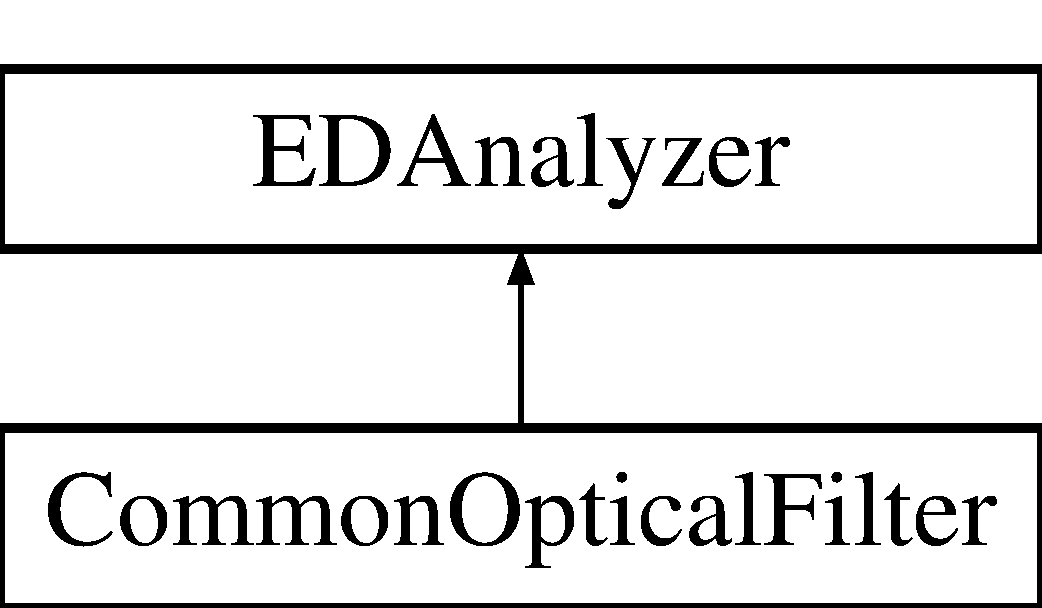
\includegraphics[height=2.000000cm]{classCommonOpticalFilter}
\end{center}
\end{figure}
\subsection*{Public Member Functions}
\begin{DoxyCompactItemize}
\item 
{\bfseries Common\+Optical\+Filter} (fhicl\+::\+Parameter\+Set const \&p)\hypertarget{classCommonOpticalFilter_a81f6d22db0a88f0d6c484130b689ceae}{}\label{classCommonOpticalFilter_a81f6d22db0a88f0d6c484130b689ceae}

\item 
{\bfseries Common\+Optical\+Filter} (\hyperlink{classCommonOpticalFilter}{Common\+Optical\+Filter} const \&)=delete\hypertarget{classCommonOpticalFilter_a45ceeadd04ac3623d214753aa21aa0f1}{}\label{classCommonOpticalFilter_a45ceeadd04ac3623d214753aa21aa0f1}

\item 
{\bfseries Common\+Optical\+Filter} (\hyperlink{classCommonOpticalFilter}{Common\+Optical\+Filter} \&\&)=delete\hypertarget{classCommonOpticalFilter_af39ba3d2916d1dab8459c5bc2fda8963}{}\label{classCommonOpticalFilter_af39ba3d2916d1dab8459c5bc2fda8963}

\item 
\hyperlink{classCommonOpticalFilter}{Common\+Optical\+Filter} \& {\bfseries operator=} (\hyperlink{classCommonOpticalFilter}{Common\+Optical\+Filter} const \&)=delete\hypertarget{classCommonOpticalFilter_a68bfc736eeb9dafa17ea51d7f8d5191a}{}\label{classCommonOpticalFilter_a68bfc736eeb9dafa17ea51d7f8d5191a}

\item 
\hyperlink{classCommonOpticalFilter}{Common\+Optical\+Filter} \& {\bfseries operator=} (\hyperlink{classCommonOpticalFilter}{Common\+Optical\+Filter} \&\&)=delete\hypertarget{classCommonOpticalFilter_aadd7bd59c546371f0d2c1b06fc187d7b}{}\label{classCommonOpticalFilter_aadd7bd59c546371f0d2c1b06fc187d7b}

\item 
void {\bfseries analyze} (art\+::\+Event const \&e) override\hypertarget{classCommonOpticalFilter_a4e474389d55dc9d143a96636a7222880}{}\label{classCommonOpticalFilter_a4e474389d55dc9d143a96636a7222880}

\item 
void {\bfseries begin\+Job} () override\hypertarget{classCommonOpticalFilter_ae1d42b367bfb18eb5a7ac9714a3c534d}{}\label{classCommonOpticalFilter_ae1d42b367bfb18eb5a7ac9714a3c534d}

\item 
void {\bfseries end\+Job} () override\hypertarget{classCommonOpticalFilter_ae29e456913b0021782b5006404b30a3f}{}\label{classCommonOpticalFilter_ae29e456913b0021782b5006404b30a3f}

\end{DoxyCompactItemize}
\subsection*{Private Attributes}
\begin{DoxyCompactItemize}
\item 
T\+Tree $\ast$ {\bfseries \+\_\+tree}\hypertarget{classCommonOpticalFilter_a505b26a587adbecb9aa55c25477bb501}{}\label{classCommonOpticalFilter_a505b26a587adbecb9aa55c25477bb501}

\item 
float {\bfseries \+\_\+nu\+\_\+e}\hypertarget{classCommonOpticalFilter_ad43c723777e80132c114cd4619b32e87}{}\label{classCommonOpticalFilter_ad43c723777e80132c114cd4619b32e87}

\item 
float {\bfseries \+\_\+elec\+\_\+e}\hypertarget{classCommonOpticalFilter_abbe2da226afe8319190c8cb51215e0f4}{}\label{classCommonOpticalFilter_abbe2da226afe8319190c8cb51215e0f4}

\item 
int {\bfseries \+\_\+nelec}\hypertarget{classCommonOpticalFilter_a3447d61fdfa4deb95e06416b6753c7a1}{}\label{classCommonOpticalFilter_a3447d61fdfa4deb95e06416b6753c7a1}

\item 
float {\bfseries \+\_\+vtx\+\_\+x}\hypertarget{classCommonOpticalFilter_a121cb598029e054d6139fbdfed346940}{}\label{classCommonOpticalFilter_a121cb598029e054d6139fbdfed346940}

\item 
float {\bfseries \+\_\+vtx\+\_\+y}\hypertarget{classCommonOpticalFilter_a61a32ad563ce3e6397b82552b044566d}{}\label{classCommonOpticalFilter_a61a32ad563ce3e6397b82552b044566d}

\item 
float {\bfseries \+\_\+vtx\+\_\+z}\hypertarget{classCommonOpticalFilter_ad1779181406830f8d5d45bbecb656092}{}\label{classCommonOpticalFilter_ad1779181406830f8d5d45bbecb656092}

\item 
float {\bfseries \+\_\+vtx\+\_\+t}\hypertarget{classCommonOpticalFilter_a328e46a9bd506d69ca9fd25090f99ee7}{}\label{classCommonOpticalFilter_a328e46a9bd506d69ca9fd25090f99ee7}

\item 
float {\bfseries \+\_\+opfilter\+\_\+pe\+\_\+beam}\hypertarget{classCommonOpticalFilter_ada83cac25db1c34a32a052f306a5d994}{}\label{classCommonOpticalFilter_ada83cac25db1c34a32a052f306a5d994}

\item 
float {\bfseries \+\_\+opfilter\+\_\+pe\+\_\+beam\+\_\+tot}\hypertarget{classCommonOpticalFilter_a89ac8cb77d6821567d434b662be81257}{}\label{classCommonOpticalFilter_a89ac8cb77d6821567d434b662be81257}

\item 
float {\bfseries \+\_\+opfilter\+\_\+pe\+\_\+veto}\hypertarget{classCommonOpticalFilter_ac4bcde210f0c9b8e672e60d6fbd99915}{}\label{classCommonOpticalFilter_ac4bcde210f0c9b8e672e60d6fbd99915}

\item 
float {\bfseries \+\_\+opfilter\+\_\+pe\+\_\+veto\+\_\+tot}\hypertarget{classCommonOpticalFilter_a18702fe52e59501c913cc7a1c5c64374}{}\label{classCommonOpticalFilter_a18702fe52e59501c913cc7a1c5c64374}

\item 
int {\bfseries \+\_\+n\+\_\+mcs}\hypertarget{classCommonOpticalFilter_a66994974ea5877849ba5ab3e8cd826de}{}\label{classCommonOpticalFilter_a66994974ea5877849ba5ab3e8cd826de}

\item 
float {\bfseries \+\_\+mcshr\+\_\+edep}\hypertarget{classCommonOpticalFilter_ab677aab9e2b4d5dafd40801c1f93a947}{}\label{classCommonOpticalFilter_ab677aab9e2b4d5dafd40801c1f93a947}

\end{DoxyCompactItemize}


The documentation for this class was generated from the following file\+:\begin{DoxyCompactItemize}
\item 
/home/travis/build/ubneutrinos/searchingfornues/\+Filters/Common\+Optical\+Filter\+\_\+module.\+cc\end{DoxyCompactItemize}

\hypertarget{classanalysis_1_1ContainmentAnalysis}{}\section{analysis\+:\+:Containment\+Analysis Class Reference}
\label{classanalysis_1_1ContainmentAnalysis}\index{analysis\+::\+Containment\+Analysis@{analysis\+::\+Containment\+Analysis}}
Inheritance diagram for analysis\+:\+:Containment\+Analysis\+:\begin{figure}[H]
\begin{center}
\leavevmode
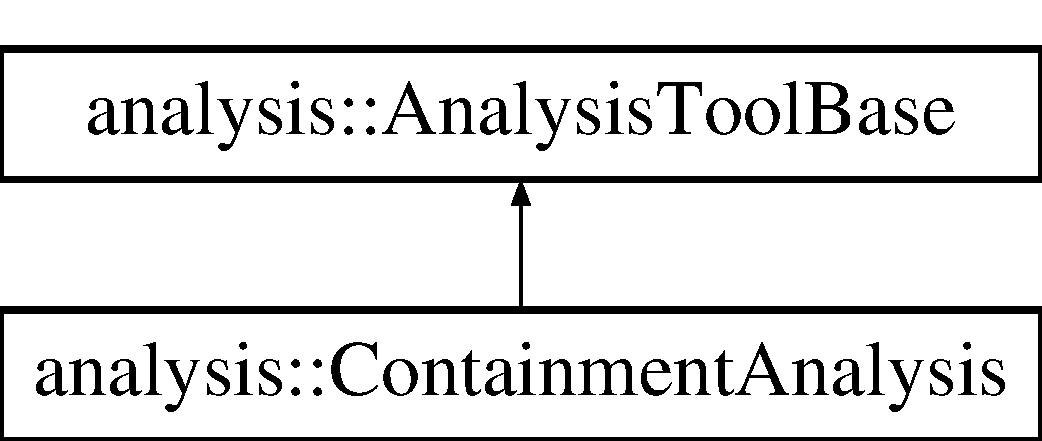
\includegraphics[height=2.000000cm]{classanalysis_1_1ContainmentAnalysis}
\end{center}
\end{figure}
\subsection*{Public Member Functions}
\begin{DoxyCompactItemize}
\item 
\hyperlink{classanalysis_1_1ContainmentAnalysis_a1544702632da81fbf99462a4099ad15e}{Containment\+Analysis} (const fhicl\+::\+Parameter\+Set \&pset)
\begin{DoxyCompactList}\small\item\em Constructor. \end{DoxyCompactList}\item 
\hyperlink{classanalysis_1_1ContainmentAnalysis_ae5f996c6ad46bc60af73f632eb3b44ae}{$\sim$\+Containment\+Analysis} ()\hypertarget{classanalysis_1_1ContainmentAnalysis_ae5f996c6ad46bc60af73f632eb3b44ae}{}\label{classanalysis_1_1ContainmentAnalysis_ae5f996c6ad46bc60af73f632eb3b44ae}

\begin{DoxyCompactList}\small\item\em Destructor. \end{DoxyCompactList}\item 
void \hyperlink{classanalysis_1_1ContainmentAnalysis_a0ea0287e139776b12c996ca624e8e8eb}{configure} (fhicl\+::\+Parameter\+Set const \&pset)
\item 
void \hyperlink{classanalysis_1_1ContainmentAnalysis_a5bcf033310f0e8f58fd6f4f46f216985}{analyze\+Event} (art\+::\+Event const \&e, bool f\+Data) override\hypertarget{classanalysis_1_1ContainmentAnalysis_a5bcf033310f0e8f58fd6f4f46f216985}{}\label{classanalysis_1_1ContainmentAnalysis_a5bcf033310f0e8f58fd6f4f46f216985}

\begin{DoxyCompactList}\small\item\em Analysis function. \end{DoxyCompactList}\item 
void \hyperlink{classanalysis_1_1ContainmentAnalysis_a6e3c839d18ff3001b46be5fde80a5d04}{analyze\+Slice} (art\+::\+Event const \&e, std\+::vector$<$ Proxy\+Pfp\+Elem\+\_\+t $>$ \&slice\+\_\+pfp\+\_\+v, bool f\+Data, bool selected) override
\begin{DoxyCompactList}\small\item\em Selection function. \end{DoxyCompactList}\item 
void \hyperlink{classanalysis_1_1ContainmentAnalysis_a468421b8ba753e554a0f96f4a912f8ff}{set\+Branches} (T\+Tree $\ast$\+\_\+tree) override\hypertarget{classanalysis_1_1ContainmentAnalysis_a468421b8ba753e554a0f96f4a912f8ff}{}\label{classanalysis_1_1ContainmentAnalysis_a468421b8ba753e554a0f96f4a912f8ff}

\begin{DoxyCompactList}\small\item\em set branches for T\+Tree \end{DoxyCompactList}\item 
void \hyperlink{classanalysis_1_1ContainmentAnalysis_a6e5a6d76850458abc42a252cec25063f}{reset\+T\+Tree} (T\+Tree $\ast$\+\_\+tree) override\hypertarget{classanalysis_1_1ContainmentAnalysis_a6e5a6d76850458abc42a252cec25063f}{}\label{classanalysis_1_1ContainmentAnalysis_a6e5a6d76850458abc42a252cec25063f}

\begin{DoxyCompactList}\small\item\em reset ttree branches \end{DoxyCompactList}\end{DoxyCompactItemize}
\subsection*{Private Member Functions}
\begin{DoxyCompactItemize}
\item 
float {\bfseries Dist\+Fiducial} (float x, float y, float z)\hypertarget{classanalysis_1_1ContainmentAnalysis_af1ae4a6e17c26624f1ffc789a1a28370}{}\label{classanalysis_1_1ContainmentAnalysis_af1ae4a6e17c26624f1ffc789a1a28370}

\item 
void {\bfseries Dist\+Fiducial\+Boundaries} (float x, float y, float z, std\+::vector$<$ std\+::vector$<$ double $>$$>$ \&dboundaries)\hypertarget{classanalysis_1_1ContainmentAnalysis_a403e7651d9e20b4f672232e05a967472}{}\label{classanalysis_1_1ContainmentAnalysis_a403e7651d9e20b4f672232e05a967472}

\end{DoxyCompactItemize}
\subsection*{Private Attributes}
\begin{DoxyCompactItemize}
\item 
art\+::\+Input\+Tag {\bfseries f\+M\+C\+Tproducer}\hypertarget{classanalysis_1_1ContainmentAnalysis_aeb708c6457c1a19e63dedc84afad8b94}{}\label{classanalysis_1_1ContainmentAnalysis_aeb708c6457c1a19e63dedc84afad8b94}

\item 
float {\bfseries \+\_\+\+FV}\hypertarget{classanalysis_1_1ContainmentAnalysis_a3ecb4264e53ae9f996a7689ae8f78541}{}\label{classanalysis_1_1ContainmentAnalysis_a3ecb4264e53ae9f996a7689ae8f78541}

\item 
float {\bfseries \+\_\+dvtx}\hypertarget{classanalysis_1_1ContainmentAnalysis_a933f497a05e85666d7e10394dc51aacd}{}\label{classanalysis_1_1ContainmentAnalysis_a933f497a05e85666d7e10394dc51aacd}

\item 
float {\bfseries \+\_\+dtrk}\hypertarget{classanalysis_1_1ContainmentAnalysis_a08c17ce66b43feddb596a78202de032c}{}\label{classanalysis_1_1ContainmentAnalysis_a08c17ce66b43feddb596a78202de032c}

\item 
std\+::vector$<$ std\+::vector$<$ double $>$ $>$ {\bfseries \+\_\+dmc\+\_\+boundary}\hypertarget{classanalysis_1_1ContainmentAnalysis_a927f6f2785545fa4cefa315c23cd1088}{}\label{classanalysis_1_1ContainmentAnalysis_a927f6f2785545fa4cefa315c23cd1088}

\item 
std\+::vector$<$ std\+::vector$<$ double $>$ $>$ {\bfseries \+\_\+dtrk\+\_\+boundary}\hypertarget{classanalysis_1_1ContainmentAnalysis_a1f4ccec0a22555c68eccf5c4295c315c}{}\label{classanalysis_1_1ContainmentAnalysis_a1f4ccec0a22555c68eccf5c4295c315c}

\item 
std\+::vector$<$ double $>$ {\bfseries \+\_\+dtrk\+\_\+x\+\_\+boundary}\hypertarget{classanalysis_1_1ContainmentAnalysis_a6b60b98bd35ca4696dd9390dc699f393}{}\label{classanalysis_1_1ContainmentAnalysis_a6b60b98bd35ca4696dd9390dc699f393}

\item 
std\+::vector$<$ double $>$ {\bfseries \+\_\+dtrk\+\_\+y\+\_\+boundary}\hypertarget{classanalysis_1_1ContainmentAnalysis_aa26415fec19cb70a4e8fafac9edb7d23}{}\label{classanalysis_1_1ContainmentAnalysis_aa26415fec19cb70a4e8fafac9edb7d23}

\item 
std\+::vector$<$ double $>$ {\bfseries \+\_\+dtrk\+\_\+z\+\_\+boundary}\hypertarget{classanalysis_1_1ContainmentAnalysis_a833a1aaeb93bec0a73ff59f25dcdcba9}{}\label{classanalysis_1_1ContainmentAnalysis_a833a1aaeb93bec0a73ff59f25dcdcba9}

\item 
std\+::vector$<$ double $>$ {\bfseries \+\_\+dshr\+\_\+x\+\_\+boundary}\hypertarget{classanalysis_1_1ContainmentAnalysis_a36e81065e3d4ea6884227063ce5047b4}{}\label{classanalysis_1_1ContainmentAnalysis_a36e81065e3d4ea6884227063ce5047b4}

\item 
std\+::vector$<$ double $>$ {\bfseries \+\_\+dshr\+\_\+y\+\_\+boundary}\hypertarget{classanalysis_1_1ContainmentAnalysis_ae623b7efd1d545fbe9d32bafac77718d}{}\label{classanalysis_1_1ContainmentAnalysis_ae623b7efd1d545fbe9d32bafac77718d}

\item 
std\+::vector$<$ double $>$ {\bfseries \+\_\+dshr\+\_\+z\+\_\+boundary}\hypertarget{classanalysis_1_1ContainmentAnalysis_ac45217df52482cc670b0ea4bd86c8257}{}\label{classanalysis_1_1ContainmentAnalysis_ac45217df52482cc670b0ea4bd86c8257}

\item 
std\+::vector$<$ double $>$ {\bfseries \+\_\+dvtx\+\_\+x\+\_\+boundary}\hypertarget{classanalysis_1_1ContainmentAnalysis_af20b04910d32f51b8ade5f0bb6558e35}{}\label{classanalysis_1_1ContainmentAnalysis_af20b04910d32f51b8ade5f0bb6558e35}

\item 
std\+::vector$<$ double $>$ {\bfseries \+\_\+dvtx\+\_\+y\+\_\+boundary}\hypertarget{classanalysis_1_1ContainmentAnalysis_ab2894eefd881547b87ed6c932b08c4df}{}\label{classanalysis_1_1ContainmentAnalysis_ab2894eefd881547b87ed6c932b08c4df}

\item 
std\+::vector$<$ double $>$ {\bfseries \+\_\+dvtx\+\_\+z\+\_\+boundary}\hypertarget{classanalysis_1_1ContainmentAnalysis_a7216bd74951faf0862964a2d41c4c280}{}\label{classanalysis_1_1ContainmentAnalysis_a7216bd74951faf0862964a2d41c4c280}

\item 
std\+::vector$<$ std\+::vector$<$ double $>$ $>$ {\bfseries \+\_\+dvtx\+\_\+boundary}\hypertarget{classanalysis_1_1ContainmentAnalysis_a063ed2f268f5c58f7823296b9aafbbe7}{}\label{classanalysis_1_1ContainmentAnalysis_a063ed2f268f5c58f7823296b9aafbbe7}

\item 
std\+::vector$<$ std\+::vector$<$ double $>$ $>$ {\bfseries \+\_\+dshr\+\_\+boundary}\hypertarget{classanalysis_1_1ContainmentAnalysis_a67f8f6bc60848aaa130169bc7be0d4e2}{}\label{classanalysis_1_1ContainmentAnalysis_a67f8f6bc60848aaa130169bc7be0d4e2}

\end{DoxyCompactItemize}


\subsection{Constructor \& Destructor Documentation}
\index{analysis\+::\+Containment\+Analysis@{analysis\+::\+Containment\+Analysis}!Containment\+Analysis@{Containment\+Analysis}}
\index{Containment\+Analysis@{Containment\+Analysis}!analysis\+::\+Containment\+Analysis@{analysis\+::\+Containment\+Analysis}}
\subsubsection[{\texorpdfstring{Containment\+Analysis(const fhicl\+::\+Parameter\+Set \&pset)}{ContainmentAnalysis(const fhicl::ParameterSet &pset)}}]{\setlength{\rightskip}{0pt plus 5cm}analysis\+::\+Containment\+Analysis\+::\+Containment\+Analysis (
\begin{DoxyParamCaption}
\item[{const fhicl\+::\+Parameter\+Set \&}]{pset}
\end{DoxyParamCaption}
)}\hypertarget{classanalysis_1_1ContainmentAnalysis_a1544702632da81fbf99462a4099ad15e}{}\label{classanalysis_1_1ContainmentAnalysis_a1544702632da81fbf99462a4099ad15e}


Constructor. 


\begin{DoxyParams}{Parameters}
{\em pset} & Constructor.\\
\hline
\end{DoxyParams}
Arguments\+:

pset -\/ Fcl parameters. 

\subsection{Member Function Documentation}
\index{analysis\+::\+Containment\+Analysis@{analysis\+::\+Containment\+Analysis}!analyze\+Slice@{analyze\+Slice}}
\index{analyze\+Slice@{analyze\+Slice}!analysis\+::\+Containment\+Analysis@{analysis\+::\+Containment\+Analysis}}
\subsubsection[{\texorpdfstring{analyze\+Slice(art\+::\+Event const \&e, std\+::vector$<$ Proxy\+Pfp\+Elem\+\_\+t $>$ \&slice\+\_\+pfp\+\_\+v, bool f\+Data, bool selected) override}{analyzeSlice(art::Event const &e, std::vector< ProxyPfpElem_t > &slice_pfp_v, bool fData, bool selected) override}}]{\setlength{\rightskip}{0pt plus 5cm}void analysis\+::\+Containment\+Analysis\+::analyze\+Slice (
\begin{DoxyParamCaption}
\item[{art\+::\+Event const \&}]{e, }
\item[{std\+::vector$<$ Proxy\+Pfp\+Elem\+\_\+t $>$ \&}]{slice\+\_\+pfp\+\_\+v, }
\item[{bool}]{f\+Data, }
\item[{bool}]{selected}
\end{DoxyParamCaption}
)\hspace{0.3cm}{\ttfamily [override]}, {\ttfamily [virtual]}}\hypertarget{classanalysis_1_1ContainmentAnalysis_a6e3c839d18ff3001b46be5fde80a5d04}{}\label{classanalysis_1_1ContainmentAnalysis_a6e3c839d18ff3001b46be5fde80a5d04}


Selection function. 

select\+Event

Arguments\+:

art\+::\+Event slice track pointer vector slice shower pointer vector 

Implements \hyperlink{classanalysis_1_1AnalysisToolBase_ac1611ea1b1a5db62a6543709ec1d2e96}{analysis\+::\+Analysis\+Tool\+Base}.

\index{analysis\+::\+Containment\+Analysis@{analysis\+::\+Containment\+Analysis}!configure@{configure}}
\index{configure@{configure}!analysis\+::\+Containment\+Analysis@{analysis\+::\+Containment\+Analysis}}
\subsubsection[{\texorpdfstring{configure(fhicl\+::\+Parameter\+Set const \&pset)}{configure(fhicl::ParameterSet const &pset)}}]{\setlength{\rightskip}{0pt plus 5cm}void analysis\+::\+Containment\+Analysis\+::configure (
\begin{DoxyParamCaption}
\item[{fhicl\+::\+Parameter\+Set const \&}]{pset}
\end{DoxyParamCaption}
)}\hypertarget{classanalysis_1_1ContainmentAnalysis_a0ea0287e139776b12c996ca624e8e8eb}{}\label{classanalysis_1_1ContainmentAnalysis_a0ea0287e139776b12c996ca624e8e8eb}
Reconfigure method.

Arguments\+:

pset -\/ Fcl parameter set. 

The documentation for this class was generated from the following file\+:\begin{DoxyCompactItemize}
\item 
/home/travis/build/ubneutrinos/searchingfornues/\+Selection/\+Analysis\+Tools/Containment\+Analysis\+\_\+tool.\+cc\end{DoxyCompactItemize}

\hypertarget{classanalysis_1_1CosmicIP}{}\section{analysis\+:\+:Cosmic\+IP Class Reference}
\label{classanalysis_1_1CosmicIP}\index{analysis\+::\+Cosmic\+IP@{analysis\+::\+Cosmic\+IP}}
Inheritance diagram for analysis\+:\+:Cosmic\+IP\+:\begin{figure}[H]
\begin{center}
\leavevmode
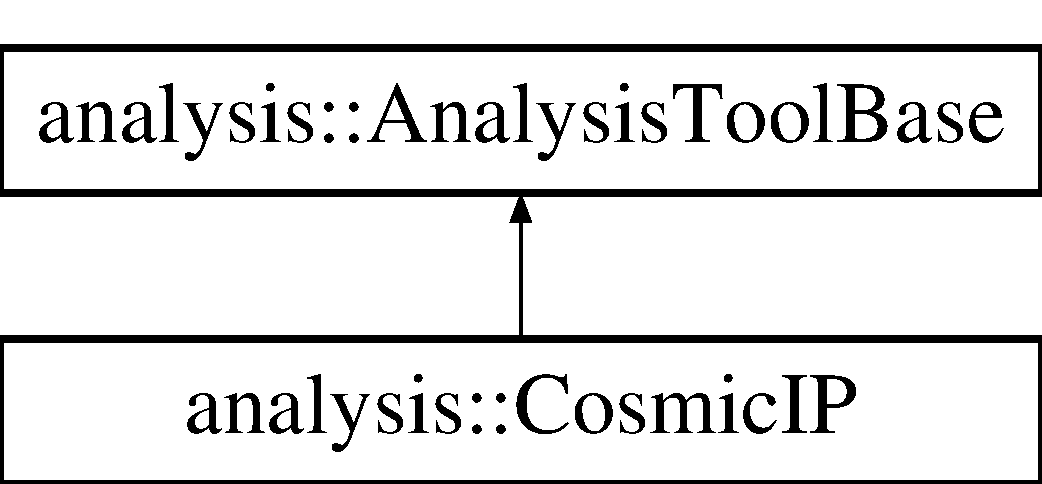
\includegraphics[height=2.000000cm]{classanalysis_1_1CosmicIP}
\end{center}
\end{figure}
\subsection*{Public Member Functions}
\begin{DoxyCompactItemize}
\item 
\hyperlink{classanalysis_1_1CosmicIP_aa34450dae6a5ea2d51520aefcc9c0e6f}{Cosmic\+IP} (const fhicl\+::\+Parameter\+Set \&pset)
\begin{DoxyCompactList}\small\item\em Constructor. \end{DoxyCompactList}\item 
\hyperlink{classanalysis_1_1CosmicIP_a7edbd55f2290fab4c766f9a749731626}{$\sim$\+Cosmic\+IP} ()\hypertarget{classanalysis_1_1CosmicIP_a7edbd55f2290fab4c766f9a749731626}{}\label{classanalysis_1_1CosmicIP_a7edbd55f2290fab4c766f9a749731626}

\begin{DoxyCompactList}\small\item\em Destructor. \end{DoxyCompactList}\item 
void \hyperlink{classanalysis_1_1CosmicIP_af2564ec208979037940ff500dea10246}{configure} (fhicl\+::\+Parameter\+Set const \&pset)
\item 
void \hyperlink{classanalysis_1_1CosmicIP_aece9b4c45c6e1771df582b2c5e40c5d5}{analyze\+Event} (art\+::\+Event const \&e, bool f\+Data) override\hypertarget{classanalysis_1_1CosmicIP_aece9b4c45c6e1771df582b2c5e40c5d5}{}\label{classanalysis_1_1CosmicIP_aece9b4c45c6e1771df582b2c5e40c5d5}

\begin{DoxyCompactList}\small\item\em Analysis function. \end{DoxyCompactList}\item 
void \hyperlink{classanalysis_1_1CosmicIP_a86c9683c997d233949d8116940918e32}{analyze\+Slice} (art\+::\+Event const \&e, std\+::vector$<$ Proxy\+Pfp\+Elem\+\_\+t $>$ \&slice\+\_\+pfp\+\_\+v, bool f\+Data, bool selected) override
\begin{DoxyCompactList}\small\item\em Analyze slice. \end{DoxyCompactList}\item 
void \hyperlink{classanalysis_1_1CosmicIP_aa676a555c1fed07fac6af653db6610ce}{set\+Branches} (T\+Tree $\ast$\+\_\+tree) override\hypertarget{classanalysis_1_1CosmicIP_aa676a555c1fed07fac6af653db6610ce}{}\label{classanalysis_1_1CosmicIP_aa676a555c1fed07fac6af653db6610ce}

\begin{DoxyCompactList}\small\item\em set branches for T\+Tree \end{DoxyCompactList}\item 
void \hyperlink{classanalysis_1_1CosmicIP_a0d921ff309b405e2a2ad668aee56c08b}{reset\+T\+Tree} (T\+Tree $\ast$\+\_\+tree) override\hypertarget{classanalysis_1_1CosmicIP_a0d921ff309b405e2a2ad668aee56c08b}{}\label{classanalysis_1_1CosmicIP_a0d921ff309b405e2a2ad668aee56c08b}

\begin{DoxyCompactList}\small\item\em reset ttree branches \end{DoxyCompactList}\end{DoxyCompactItemize}
\subsection*{Private Attributes}
\begin{DoxyCompactItemize}
\item 
art\+::\+Input\+Tag {\bfseries f\+P\+F\+Pproducer}\hypertarget{classanalysis_1_1CosmicIP_a9b6be9be6fb0f4bee6f49af8b1b68860}{}\label{classanalysis_1_1CosmicIP_a9b6be9be6fb0f4bee6f49af8b1b68860}

\item 
art\+::\+Input\+Tag {\bfseries f\+Space\+Pointproducer}\hypertarget{classanalysis_1_1CosmicIP_ae185a274823b69244a40f338300bbc02}{}\label{classanalysis_1_1CosmicIP_ae185a274823b69244a40f338300bbc02}

\item 
float {\bfseries f\+Trk\+Shr\+Score}\hypertarget{classanalysis_1_1CosmicIP_ad2a113ce491c0b974a96a9f6c639e5cf}{}\label{classanalysis_1_1CosmicIP_ad2a113ce491c0b974a96a9f6c639e5cf}

\item 
float {\bfseries \+\_\+\+Cosmic\+IP}\hypertarget{classanalysis_1_1CosmicIP_ab4c8609cc3b23ad7607e3cc3eeb9d38e}{}\label{classanalysis_1_1CosmicIP_ab4c8609cc3b23ad7607e3cc3eeb9d38e}

\end{DoxyCompactItemize}


\subsection{Constructor \& Destructor Documentation}
\index{analysis\+::\+Cosmic\+IP@{analysis\+::\+Cosmic\+IP}!Cosmic\+IP@{Cosmic\+IP}}
\index{Cosmic\+IP@{Cosmic\+IP}!analysis\+::\+Cosmic\+IP@{analysis\+::\+Cosmic\+IP}}
\subsubsection[{\texorpdfstring{Cosmic\+I\+P(const fhicl\+::\+Parameter\+Set \&pset)}{CosmicIP(const fhicl::ParameterSet &pset)}}]{\setlength{\rightskip}{0pt plus 5cm}analysis\+::\+Cosmic\+I\+P\+::\+Cosmic\+IP (
\begin{DoxyParamCaption}
\item[{const fhicl\+::\+Parameter\+Set \&}]{p}
\end{DoxyParamCaption}
)}\hypertarget{classanalysis_1_1CosmicIP_aa34450dae6a5ea2d51520aefcc9c0e6f}{}\label{classanalysis_1_1CosmicIP_aa34450dae6a5ea2d51520aefcc9c0e6f}


Constructor. 


\begin{DoxyParams}{Parameters}
{\em pset} & Constructor.\\
\hline
\end{DoxyParams}
Arguments\+:

pset -\/ Fcl parameters. 

\subsection{Member Function Documentation}
\index{analysis\+::\+Cosmic\+IP@{analysis\+::\+Cosmic\+IP}!analyze\+Slice@{analyze\+Slice}}
\index{analyze\+Slice@{analyze\+Slice}!analysis\+::\+Cosmic\+IP@{analysis\+::\+Cosmic\+IP}}
\subsubsection[{\texorpdfstring{analyze\+Slice(art\+::\+Event const \&e, std\+::vector$<$ Proxy\+Pfp\+Elem\+\_\+t $>$ \&slice\+\_\+pfp\+\_\+v, bool f\+Data, bool selected) override}{analyzeSlice(art::Event const &e, std::vector< ProxyPfpElem_t > &slice_pfp_v, bool fData, bool selected) override}}]{\setlength{\rightskip}{0pt plus 5cm}void analysis\+::\+Cosmic\+I\+P\+::analyze\+Slice (
\begin{DoxyParamCaption}
\item[{art\+::\+Event const \&}]{e, }
\item[{std\+::vector$<$ Proxy\+Pfp\+Elem\+\_\+t $>$ \&}]{slice\+\_\+pfp\+\_\+v, }
\item[{bool}]{f\+Data, }
\item[{bool}]{selected}
\end{DoxyParamCaption}
)\hspace{0.3cm}{\ttfamily [override]}, {\ttfamily [virtual]}}\hypertarget{classanalysis_1_1CosmicIP_a86c9683c997d233949d8116940918e32}{}\label{classanalysis_1_1CosmicIP_a86c9683c997d233949d8116940918e32}


Analyze slice. 

Reconfigure method.

Arguments\+:

pset -\/ Fcl parameter set. 

Implements \hyperlink{classanalysis_1_1AnalysisToolBase_ac1611ea1b1a5db62a6543709ec1d2e96}{analysis\+::\+Analysis\+Tool\+Base}.

\index{analysis\+::\+Cosmic\+IP@{analysis\+::\+Cosmic\+IP}!configure@{configure}}
\index{configure@{configure}!analysis\+::\+Cosmic\+IP@{analysis\+::\+Cosmic\+IP}}
\subsubsection[{\texorpdfstring{configure(fhicl\+::\+Parameter\+Set const \&pset)}{configure(fhicl::ParameterSet const &pset)}}]{\setlength{\rightskip}{0pt plus 5cm}void analysis\+::\+Cosmic\+I\+P\+::configure (
\begin{DoxyParamCaption}
\item[{fhicl\+::\+Parameter\+Set const \&}]{p}
\end{DoxyParamCaption}
)}\hypertarget{classanalysis_1_1CosmicIP_af2564ec208979037940ff500dea10246}{}\label{classanalysis_1_1CosmicIP_af2564ec208979037940ff500dea10246}
Reconfigure method.

Arguments\+:

pset -\/ Fcl parameter set. 

The documentation for this class was generated from the following file\+:\begin{DoxyCompactItemize}
\item 
/home/travis/build/ubneutrinos/searchingfornues/\+Selection/\+Analysis\+Tools/Cosmic\+I\+P\+\_\+tool.\+cc\end{DoxyCompactItemize}

\hypertarget{classCosmicRejection}{\section{Cosmic\-Rejection Class Reference}
\label{classCosmicRejection}\index{Cosmic\-Rejection@{Cosmic\-Rejection}}
}
Inheritance diagram for Cosmic\-Rejection\-:\begin{figure}[H]
\begin{center}
\leavevmode
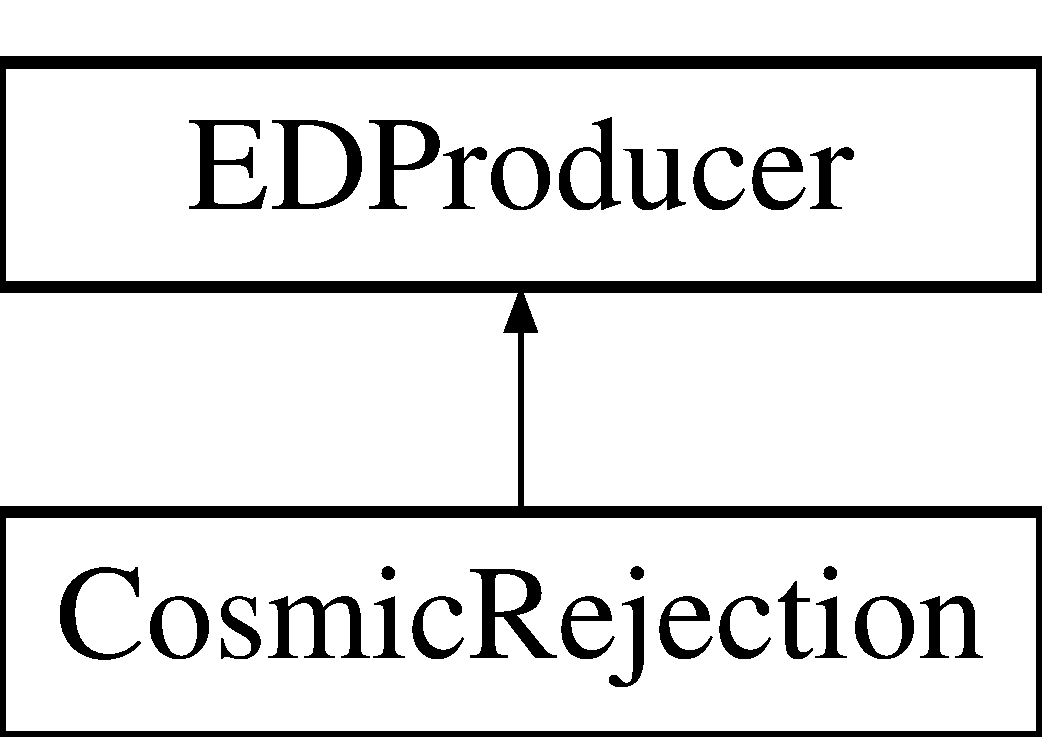
\includegraphics[height=2.000000cm]{classCosmicRejection}
\end{center}
\end{figure}
\subsection*{Public Member Functions}
\begin{DoxyCompactItemize}
\item 
\hypertarget{classCosmicRejection_a7663d784ec40b8a3ba79b76b775118c7}{{\bfseries Cosmic\-Rejection} (fhicl\-::\-Parameter\-Set const \&p)}\label{classCosmicRejection_a7663d784ec40b8a3ba79b76b775118c7}

\item 
\hypertarget{classCosmicRejection_aa06f3640dbccac91b299101b712bbe97}{{\bfseries Cosmic\-Rejection} (\hyperlink{classCosmicRejection}{Cosmic\-Rejection} const \&)=delete}\label{classCosmicRejection_aa06f3640dbccac91b299101b712bbe97}

\item 
\hypertarget{classCosmicRejection_a391a622a1cfb9b03d3298d046e850f63}{{\bfseries Cosmic\-Rejection} (\hyperlink{classCosmicRejection}{Cosmic\-Rejection} \&\&)=delete}\label{classCosmicRejection_a391a622a1cfb9b03d3298d046e850f63}

\item 
\hypertarget{classCosmicRejection_a49fdc618e61833a84f5f548a16dab324}{\hyperlink{classCosmicRejection}{Cosmic\-Rejection} \& {\bfseries operator=} (\hyperlink{classCosmicRejection}{Cosmic\-Rejection} const \&)=delete}\label{classCosmicRejection_a49fdc618e61833a84f5f548a16dab324}

\item 
\hypertarget{classCosmicRejection_a07294b34f21bfa92ece444820e96faac}{\hyperlink{classCosmicRejection}{Cosmic\-Rejection} \& {\bfseries operator=} (\hyperlink{classCosmicRejection}{Cosmic\-Rejection} \&\&)=delete}\label{classCosmicRejection_a07294b34f21bfa92ece444820e96faac}

\item 
\hypertarget{classCosmicRejection_a5275aff5d81db9b43574ea13d1f15d12}{void {\bfseries produce} (art\-::\-Event \&e) override}\label{classCosmicRejection_a5275aff5d81db9b43574ea13d1f15d12}

\end{DoxyCompactItemize}
\subsection*{Private Member Functions}
\begin{DoxyCompactItemize}
\item 
\hypertarget{classCosmicRejection_a3d08aca297afc5331fdbab328b356137}{void {\bfseries Add\-Daughters} (const art\-::\-Ptr$<$ recob\-::\-P\-F\-Particle $>$ \&pfp, const art\-::\-Valid\-Handle$<$ std\-::vector$<$ recob\-::\-P\-F\-Particle $>$ $>$ \&pfp\-\_\-h, std\-::vector$<$ art\-::\-Ptr$<$ recob\-::\-P\-F\-Particle $>$ $>$ \&pfp\-\_\-v)}\label{classCosmicRejection_a3d08aca297afc5331fdbab328b356137}

\item 
\hypertarget{classCosmicRejection_afc2a715c5cf89aa6c20faebe5b5f7119}{bool {\bfseries Obvious\-Cosmic} (const std\-::vector$<$ art\-::\-Ptr$<$ recob\-::\-Track $>$ $>$ \&pfp\-\_\-track\-\_\-assn\-\_\-v)}\label{classCosmicRejection_afc2a715c5cf89aa6c20faebe5b5f7119}

\item 
\hypertarget{classCosmicRejection_a1538163eeb6a0ed22f6bba844952f1f0}{bool {\bfseries Track\-In\-Time} (const art\-::\-Ptr$<$ recob\-::\-Track $>$ \&pfp\-\_\-track\-\_\-assn\-\_\-v)}\label{classCosmicRejection_a1538163eeb6a0ed22f6bba844952f1f0}

\end{DoxyCompactItemize}
\subsection*{Private Attributes}
\begin{DoxyCompactItemize}
\item 
\hypertarget{classCosmicRejection_a032c55a459e56180eb0041033fa3ef34}{std\-::string {\bfseries f\-P\-F\-Pproducer}}\label{classCosmicRejection_a032c55a459e56180eb0041033fa3ef34}

\item 
\hypertarget{classCosmicRejection_a8f638302d646f661ce8926cf5442783f}{std\-::string {\bfseries f\-Space\-Pointproducer}}\label{classCosmicRejection_a8f638302d646f661ce8926cf5442783f}

\item 
\hypertarget{classCosmicRejection_a89d060de9ac73f2847caf864c6eed691}{std\-::unique\-\_\-ptr\\*
$<$ \hyperlink{classflashmatch_1_1FlashMatchingToolBase}{flashmatch\-::\-Flash\-Matching\-Tool\-Base} $>$ \hyperlink{classCosmicRejection_a89d060de9ac73f2847caf864c6eed691}{\-\_\-flashmatch\-Tool}}\label{classCosmicRejection_a89d060de9ac73f2847caf864c6eed691}

\begin{DoxyCompactList}\small\item\em The slice id tool. \end{DoxyCompactList}\item 
\hypertarget{classCosmicRejection_a3c8cc182ac836bfe075b7ff7958dc691}{T\-Tree $\ast$ {\bfseries \-\_\-tree}}\label{classCosmicRejection_a3c8cc182ac836bfe075b7ff7958dc691}

\item 
\hypertarget{classCosmicRejection_a67ae851b53fcd9254bafa834368aacf9}{float {\bfseries \-\_\-score}}\label{classCosmicRejection_a67ae851b53fcd9254bafa834368aacf9}

\item 
\hypertarget{classCosmicRejection_a2a52872e6ac61b0948c0d6a27f49f827}{float {\bfseries \-\_\-best\-\_\-score}}\label{classCosmicRejection_a2a52872e6ac61b0948c0d6a27f49f827}

\item 
\hypertarget{classCosmicRejection_a33b7e7bb2de6fffbb340b9b061904dca}{float {\bfseries \-\_\-xe}}\label{classCosmicRejection_a33b7e7bb2de6fffbb340b9b061904dca}

\item 
\hypertarget{classCosmicRejection_ac33522cd488a11284d2c1041114842e2}{float {\bfseries \-\_\-ye}}\label{classCosmicRejection_ac33522cd488a11284d2c1041114842e2}

\item 
\hypertarget{classCosmicRejection_a577912c55709ae4899aa9381034babe4}{float {\bfseries \-\_\-ze}}\label{classCosmicRejection_a577912c55709ae4899aa9381034babe4}

\item 
\hypertarget{classCosmicRejection_a3d9f8e6b3c8b618de508fe4fc0d481bd}{float {\bfseries \-\_\-xs}}\label{classCosmicRejection_a3d9f8e6b3c8b618de508fe4fc0d481bd}

\item 
\hypertarget{classCosmicRejection_aaec4fa1fe29d24b18e27bb90f23f5615}{float {\bfseries \-\_\-ys}}\label{classCosmicRejection_aaec4fa1fe29d24b18e27bb90f23f5615}

\item 
\hypertarget{classCosmicRejection_af6eb1f4fc0e76bd7767fee1853ea9df0}{float {\bfseries \-\_\-zs}}\label{classCosmicRejection_af6eb1f4fc0e76bd7767fee1853ea9df0}

\item 
\hypertarget{classCosmicRejection_a67ce3a575fc7851f38c25e72b0fa5ba7}{int {\bfseries \-\_\-obvious}}\label{classCosmicRejection_a67ce3a575fc7851f38c25e72b0fa5ba7}

\item 
\hypertarget{classCosmicRejection_ad779ba81aabfa19efc0bb5ff510efc1f}{std\-::vector$<$ float $>$ {\bfseries \-\_\-pe\-Spectrum}}\label{classCosmicRejection_ad779ba81aabfa19efc0bb5ff510efc1f}

\item 
\hypertarget{classCosmicRejection_a8a5730ec0de3b8a24c74a68a0da49933}{std\-::vector$<$ float $>$ {\bfseries \-\_\-pe\-Hypothesis}}\label{classCosmicRejection_a8a5730ec0de3b8a24c74a68a0da49933}

\item 
\hypertarget{classCosmicRejection_ab7db5d48133461aa8039101823987404}{std\-::map$<$ unsigned int, \\*
unsigned int $>$ {\bfseries \-\_\-pfpmap}}\label{classCosmicRejection_ab7db5d48133461aa8039101823987404}

\end{DoxyCompactItemize}


The documentation for this class was generated from the following file\-:\begin{DoxyCompactItemize}
\item 
/home/travis/build/ubneutrinos/searchingfornues/\-Flash\-Matching/Cosmic\-Rejection\-\_\-module.\-cc\end{DoxyCompactItemize}

\hypertarget{classanalysis_1_1CRTApproachAnalysis}{\section{analysis\-:\-:C\-R\-T\-Approach\-Analysis Class Reference}
\label{classanalysis_1_1CRTApproachAnalysis}\index{analysis\-::\-C\-R\-T\-Approach\-Analysis@{analysis\-::\-C\-R\-T\-Approach\-Analysis}}
}
Inheritance diagram for analysis\-:\-:C\-R\-T\-Approach\-Analysis\-:\begin{figure}[H]
\begin{center}
\leavevmode
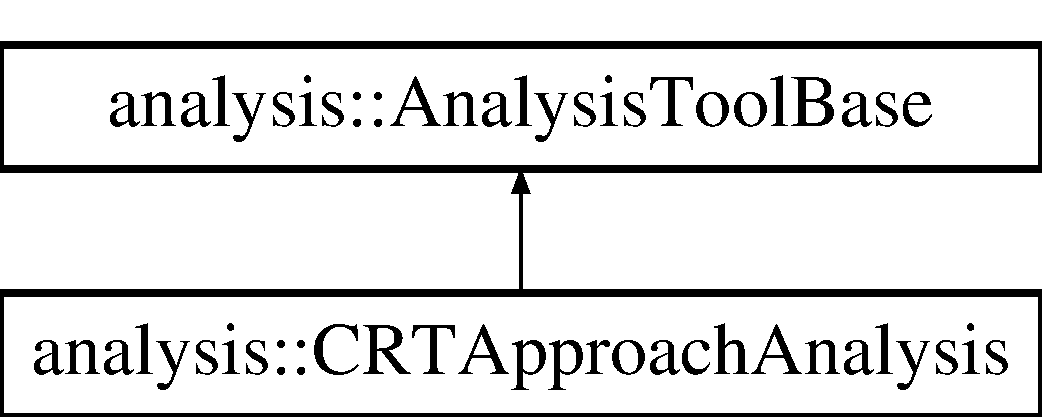
\includegraphics[height=2.000000cm]{classanalysis_1_1CRTApproachAnalysis}
\end{center}
\end{figure}
\subsection*{Public Member Functions}
\begin{DoxyCompactItemize}
\item 
\hyperlink{classanalysis_1_1CRTApproachAnalysis_a15b3a1fc6bdd4cea8e96d604ea40e061}{C\-R\-T\-Approach\-Analysis} (const fhicl\-::\-Parameter\-Set \&pset)
\begin{DoxyCompactList}\small\item\em Constructor. \end{DoxyCompactList}\item 
\hypertarget{classanalysis_1_1CRTApproachAnalysis_a4a25552da3eaba21e3d17b78d10c4bce}{\hyperlink{classanalysis_1_1CRTApproachAnalysis_a4a25552da3eaba21e3d17b78d10c4bce}{$\sim$\-C\-R\-T\-Approach\-Analysis} ()}\label{classanalysis_1_1CRTApproachAnalysis_a4a25552da3eaba21e3d17b78d10c4bce}

\begin{DoxyCompactList}\small\item\em Destructor. \end{DoxyCompactList}\item 
void \hyperlink{classanalysis_1_1CRTApproachAnalysis_a6e86e8f45b26d8712cd5749b2e983a10}{configure} (fhicl\-::\-Parameter\-Set const \&pset)
\item 
\hypertarget{classanalysis_1_1CRTApproachAnalysis_ad367db2555c9f7b34b9854e3e21bf9ca}{void \hyperlink{classanalysis_1_1CRTApproachAnalysis_ad367db2555c9f7b34b9854e3e21bf9ca}{analyze\-Event} (art\-::\-Event const \&e, bool f\-Data) override}\label{classanalysis_1_1CRTApproachAnalysis_ad367db2555c9f7b34b9854e3e21bf9ca}

\begin{DoxyCompactList}\small\item\em Analysis function. \end{DoxyCompactList}\item 
\hypertarget{classanalysis_1_1CRTApproachAnalysis_a1ec2e53aa488645ad8c7ba625699d394}{void \hyperlink{classanalysis_1_1CRTApproachAnalysis_a1ec2e53aa488645ad8c7ba625699d394}{analyze\-Slice} (art\-::\-Event const \&e, std\-::vector$<$ Proxy\-Pfp\-Elem\-\_\-t $>$ \&slice\-\_\-pfp\-\_\-v, bool f\-Data, bool selected) override}\label{classanalysis_1_1CRTApproachAnalysis_a1ec2e53aa488645ad8c7ba625699d394}

\begin{DoxyCompactList}\small\item\em Analyze slice. \end{DoxyCompactList}\item 
\hypertarget{classanalysis_1_1CRTApproachAnalysis_a457c95415578481a7c92b6b676b39550}{void \hyperlink{classanalysis_1_1CRTApproachAnalysis_a457c95415578481a7c92b6b676b39550}{set\-Branches} (T\-Tree $\ast$\-\_\-tree) override}\label{classanalysis_1_1CRTApproachAnalysis_a457c95415578481a7c92b6b676b39550}

\begin{DoxyCompactList}\small\item\em set branches for T\-Tree \end{DoxyCompactList}\item 
\hypertarget{classanalysis_1_1CRTApproachAnalysis_a82b4234fdad706613efdb29fb89e8581}{void \hyperlink{classanalysis_1_1CRTApproachAnalysis_a82b4234fdad706613efdb29fb89e8581}{reset\-T\-Tree} (T\-Tree $\ast$\-\_\-tree) override}\label{classanalysis_1_1CRTApproachAnalysis_a82b4234fdad706613efdb29fb89e8581}

\begin{DoxyCompactList}\small\item\em reset ttree branches \end{DoxyCompactList}\end{DoxyCompactItemize}
\subsection*{Private Member Functions}
\begin{DoxyCompactItemize}
\item 
\hypertarget{classanalysis_1_1CRTApproachAnalysis_aad7633096ac24f335774fee3908b5cb7}{double {\bfseries Point2\-Point\-Distance} (const T\-Vector3 \&nuvtx, T\-Vector3 \&tagged\-Track\-Spt)}\label{classanalysis_1_1CRTApproachAnalysis_aad7633096ac24f335774fee3908b5cb7}

\item 
\hypertarget{classanalysis_1_1CRTApproachAnalysis_abff1e05cb70a3d88d03d3ef670c114e7}{void {\bfseries Reset} ()}\label{classanalysis_1_1CRTApproachAnalysis_abff1e05cb70a3d88d03d3ef670c114e7}

\end{DoxyCompactItemize}
\subsection*{Private Attributes}
\begin{DoxyCompactItemize}
\item 
\hypertarget{classanalysis_1_1CRTApproachAnalysis_a12b38e09d85981f08ad84129e29a1bb1}{std\-::string {\bfseries f\-Track\-Assn\-Module\-Label}}\label{classanalysis_1_1CRTApproachAnalysis_a12b38e09d85981f08ad84129e29a1bb1}

\item 
\hypertarget{classanalysis_1_1CRTApproachAnalysis_a5f5bbad3eba57db3d804ec3b41127f85}{T\-Random3 {\bfseries rand}}\label{classanalysis_1_1CRTApproachAnalysis_a5f5bbad3eba57db3d804ec3b41127f85}

\item 
\hypertarget{classanalysis_1_1CRTApproachAnalysis_accc36452a567135cbfa015703337c60a}{Double\-\_\-t {\bfseries fid\-Vol\-Min\-X} = 0}\label{classanalysis_1_1CRTApproachAnalysis_accc36452a567135cbfa015703337c60a}

\item 
\hypertarget{classanalysis_1_1CRTApproachAnalysis_a7474b01aa6d531f0f9c0f1be52653a8f}{Double\-\_\-t {\bfseries fid\-Vol\-Max\-X} = 256}\label{classanalysis_1_1CRTApproachAnalysis_a7474b01aa6d531f0f9c0f1be52653a8f}

\item 
\hypertarget{classanalysis_1_1CRTApproachAnalysis_ae35fc4d3ae6977ac15f596c183bd1f79}{Double\-\_\-t {\bfseries fid\-Vol\-Min\-Y} = -\/116}\label{classanalysis_1_1CRTApproachAnalysis_ae35fc4d3ae6977ac15f596c183bd1f79}

\item 
\hypertarget{classanalysis_1_1CRTApproachAnalysis_a019a6fcc09840861b82618c06135ce15}{Double\-\_\-t {\bfseries fid\-Vol\-Max\-Y} = 116}\label{classanalysis_1_1CRTApproachAnalysis_a019a6fcc09840861b82618c06135ce15}

\item 
\hypertarget{classanalysis_1_1CRTApproachAnalysis_a4ee0c11b425276f68d1688847cb7ddac}{Double\-\_\-t {\bfseries fid\-Vol\-Min\-Z} = 0}\label{classanalysis_1_1CRTApproachAnalysis_a4ee0c11b425276f68d1688847cb7ddac}

\item 
\hypertarget{classanalysis_1_1CRTApproachAnalysis_ae20e417072170f7537ba9fb0ba79bb9f}{Double\-\_\-t {\bfseries fid\-Vol\-Max\-Z} = 1030}\label{classanalysis_1_1CRTApproachAnalysis_ae20e417072170f7537ba9fb0ba79bb9f}

\item 
\hypertarget{classanalysis_1_1CRTApproachAnalysis_a2a0fd90f28cd4bda2adff71161fae0c2}{int {\bfseries \-\_\-run}}\label{classanalysis_1_1CRTApproachAnalysis_a2a0fd90f28cd4bda2adff71161fae0c2}

\item 
\hypertarget{classanalysis_1_1CRTApproachAnalysis_a1f8e38875458641b450311bddbe7957f}{int {\bfseries \-\_\-sub}}\label{classanalysis_1_1CRTApproachAnalysis_a1f8e38875458641b450311bddbe7957f}

\item 
\hypertarget{classanalysis_1_1CRTApproachAnalysis_a5db8655e8fa9f698d79da2411e87b122}{int {\bfseries \-\_\-evt}}\label{classanalysis_1_1CRTApproachAnalysis_a5db8655e8fa9f698d79da2411e87b122}

\item 
\hypertarget{classanalysis_1_1CRTApproachAnalysis_ab0441c2d2764572303bfcb5615688bc3}{int {\bfseries \-\_\-n\-Assn\-Cosmics}}\label{classanalysis_1_1CRTApproachAnalysis_ab0441c2d2764572303bfcb5615688bc3}

\item 
\hypertarget{classanalysis_1_1CRTApproachAnalysis_aa844f3fc81f25d83934422f5a151e7bd}{Double\-\_\-t {\bfseries \-\_\-t0\-Cosm\-\_\-v} \mbox{[}k\-Max\-Cosm\mbox{]}}\label{classanalysis_1_1CRTApproachAnalysis_aa844f3fc81f25d83934422f5a151e7bd}

\item 
\hypertarget{classanalysis_1_1CRTApproachAnalysis_ac6097ff74e2b99cc2bfb91b1169f65e0}{Double\-\_\-t {\bfseries \-\_\-t0times\-V\-Cosm\-\_\-v} \mbox{[}k\-Max\-Cosm\mbox{]}}\label{classanalysis_1_1CRTApproachAnalysis_ac6097ff74e2b99cc2bfb91b1169f65e0}

\item 
\hypertarget{classanalysis_1_1CRTApproachAnalysis_a6dfb88d2ef50eccb37f49162e80d21ff}{Double\-\_\-t {\bfseries \-\_\-x\-Start\-Cosm\-\_\-v} \mbox{[}k\-Max\-Cosm\mbox{]}}\label{classanalysis_1_1CRTApproachAnalysis_a6dfb88d2ef50eccb37f49162e80d21ff}

\item 
\hypertarget{classanalysis_1_1CRTApproachAnalysis_a102620da5e5b5b12853b58579d7fdfec}{Double\-\_\-t {\bfseries \-\_\-y\-Start\-Cosm\-\_\-v} \mbox{[}k\-Max\-Cosm\mbox{]}}\label{classanalysis_1_1CRTApproachAnalysis_a102620da5e5b5b12853b58579d7fdfec}

\item 
\hypertarget{classanalysis_1_1CRTApproachAnalysis_ac2db101d87a992c190b15e8ed4e1aea4}{Double\-\_\-t {\bfseries \-\_\-z\-Start\-Cosm\-\_\-v} \mbox{[}k\-Max\-Cosm\mbox{]}}\label{classanalysis_1_1CRTApproachAnalysis_ac2db101d87a992c190b15e8ed4e1aea4}

\item 
\hypertarget{classanalysis_1_1CRTApproachAnalysis_a524668a4106c0c028420d6d8c8474c82}{Double\-\_\-t {\bfseries \-\_\-x\-End\-Cosm\-\_\-v} \mbox{[}k\-Max\-Cosm\mbox{]}}\label{classanalysis_1_1CRTApproachAnalysis_a524668a4106c0c028420d6d8c8474c82}

\item 
\hypertarget{classanalysis_1_1CRTApproachAnalysis_ad026897cd32d8f730802077de60a5d8a}{Double\-\_\-t {\bfseries \-\_\-y\-End\-Cosm\-\_\-v} \mbox{[}k\-Max\-Cosm\mbox{]}}\label{classanalysis_1_1CRTApproachAnalysis_ad026897cd32d8f730802077de60a5d8a}

\item 
\hypertarget{classanalysis_1_1CRTApproachAnalysis_a8fc6f8358bc0de2d306b6f41d0e21906}{Double\-\_\-t {\bfseries \-\_\-z\-End\-Cosm\-\_\-v} \mbox{[}k\-Max\-Cosm\mbox{]}}\label{classanalysis_1_1CRTApproachAnalysis_a8fc6f8358bc0de2d306b6f41d0e21906}

\item 
\hypertarget{classanalysis_1_1CRTApproachAnalysis_ad585f7838f5bdf56693153c205017c84}{Double\-\_\-t {\bfseries \-\_\-reco\-Nu\-\_\-vtx\-\_\-x}}\label{classanalysis_1_1CRTApproachAnalysis_ad585f7838f5bdf56693153c205017c84}

\item 
\hypertarget{classanalysis_1_1CRTApproachAnalysis_a4e449ee6a7df29e1184d32726ef0ecd5}{Double\-\_\-t {\bfseries \-\_\-reco\-Nu\-\_\-vtx\-\_\-y}}\label{classanalysis_1_1CRTApproachAnalysis_a4e449ee6a7df29e1184d32726ef0ecd5}

\item 
\hypertarget{classanalysis_1_1CRTApproachAnalysis_a1eee11a11aea1face9c4363e1edbf478}{Double\-\_\-t {\bfseries \-\_\-reco\-Nu\-\_\-vtx\-\_\-z}}\label{classanalysis_1_1CRTApproachAnalysis_a1eee11a11aea1face9c4363e1edbf478}

\item 
\hypertarget{classanalysis_1_1CRTApproachAnalysis_ad78df4e2993acd4a0219fae8cd88274a}{Double\-\_\-t {\bfseries \-\_\-t0\-\_\-nu\-\_\-cosmic}}\label{classanalysis_1_1CRTApproachAnalysis_ad78df4e2993acd4a0219fae8cd88274a}

\item 
\hypertarget{classanalysis_1_1CRTApproachAnalysis_aa92e0f8db385b70d95c3ec2892e90230}{Double\-\_\-t {\bfseries \-\_\-nu\-\_\-cosmic\-\_\-x}}\label{classanalysis_1_1CRTApproachAnalysis_aa92e0f8db385b70d95c3ec2892e90230}

\item 
\hypertarget{classanalysis_1_1CRTApproachAnalysis_a2610dbf0198ec084b0f35cfe8f1a659e}{Double\-\_\-t {\bfseries \-\_\-nu\-\_\-cosmic\-\_\-y}}\label{classanalysis_1_1CRTApproachAnalysis_a2610dbf0198ec084b0f35cfe8f1a659e}

\item 
\hypertarget{classanalysis_1_1CRTApproachAnalysis_a3c1530d4b2b73b1d34001c6db1a16570}{Double\-\_\-t {\bfseries \-\_\-nu\-\_\-cosmic\-\_\-z}}\label{classanalysis_1_1CRTApproachAnalysis_a3c1530d4b2b73b1d34001c6db1a16570}

\item 
\hypertarget{classanalysis_1_1CRTApproachAnalysis_ac48e60fb739d260ec5e82eb00ecfe97a}{Double\-\_\-t {\bfseries \-\_\-nu\-\_\-cosmic\-\_\-\-Length}}\label{classanalysis_1_1CRTApproachAnalysis_ac48e60fb739d260ec5e82eb00ecfe97a}

\item 
\hypertarget{classanalysis_1_1CRTApproachAnalysis_af38c45178405c95d92ff6279ced5c701}{Double\-\_\-t {\bfseries \-\_\-nu\-\_\-cosmic\-\_\-\-Start\-\_\-x}}\label{classanalysis_1_1CRTApproachAnalysis_af38c45178405c95d92ff6279ced5c701}

\item 
\hypertarget{classanalysis_1_1CRTApproachAnalysis_a1457a5b6faa31a0a44ea1678ad682eaa}{Double\-\_\-t {\bfseries \-\_\-nu\-\_\-cosmic\-\_\-\-Start\-\_\-y}}\label{classanalysis_1_1CRTApproachAnalysis_a1457a5b6faa31a0a44ea1678ad682eaa}

\item 
\hypertarget{classanalysis_1_1CRTApproachAnalysis_aa0904cbaeed5b3d6d84320d2f539b19c}{Double\-\_\-t {\bfseries \-\_\-nu\-\_\-cosmic\-\_\-\-Start\-\_\-z}}\label{classanalysis_1_1CRTApproachAnalysis_aa0904cbaeed5b3d6d84320d2f539b19c}

\item 
\hypertarget{classanalysis_1_1CRTApproachAnalysis_ae1a5dc0a4103b34748b9b0fca0cc35ec}{Double\-\_\-t {\bfseries \-\_\-nu\-\_\-cosmic\-\_\-\-End\-\_\-x}}\label{classanalysis_1_1CRTApproachAnalysis_ae1a5dc0a4103b34748b9b0fca0cc35ec}

\item 
\hypertarget{classanalysis_1_1CRTApproachAnalysis_aef5db32cc43c59363d02eb08ef71eff8}{Double\-\_\-t {\bfseries \-\_\-nu\-\_\-cosmic\-\_\-\-End\-\_\-y}}\label{classanalysis_1_1CRTApproachAnalysis_aef5db32cc43c59363d02eb08ef71eff8}

\item 
\hypertarget{classanalysis_1_1CRTApproachAnalysis_a49422c2a863bd2577169f4b1ad97b3d7}{Double\-\_\-t {\bfseries \-\_\-nu\-\_\-cosmic\-\_\-\-End\-\_\-z}}\label{classanalysis_1_1CRTApproachAnalysis_a49422c2a863bd2577169f4b1ad97b3d7}

\item 
\hypertarget{classanalysis_1_1CRTApproachAnalysis_a4d3e71a81124da5d86c4f3ac411eeba4}{Double\-\_\-t {\bfseries \-\_\-nu\-\_\-cosmic\-\_\-\-Track\-I\-D}}\label{classanalysis_1_1CRTApproachAnalysis_a4d3e71a81124da5d86c4f3ac411eeba4}

\item 
\hypertarget{classanalysis_1_1CRTApproachAnalysis_a6164e24d25a2646137c6e75db535caae}{Double\-\_\-t {\bfseries \-\_\-closest\-Nu\-Cosmic\-Dist} = 999999999.}\label{classanalysis_1_1CRTApproachAnalysis_a6164e24d25a2646137c6e75db535caae}

\item 
\hypertarget{classanalysis_1_1CRTApproachAnalysis_ad1fc1c98e161ce03efc93c28b39d5bec}{Double\-\_\-t {\bfseries \-\_\-rand\-\_\-vtx\-\_\-x}}\label{classanalysis_1_1CRTApproachAnalysis_ad1fc1c98e161ce03efc93c28b39d5bec}

\item 
\hypertarget{classanalysis_1_1CRTApproachAnalysis_af99a7fcad58c4da01ffc04e63c312183}{Double\-\_\-t {\bfseries \-\_\-rand\-\_\-vtx\-\_\-y}}\label{classanalysis_1_1CRTApproachAnalysis_af99a7fcad58c4da01ffc04e63c312183}

\item 
\hypertarget{classanalysis_1_1CRTApproachAnalysis_ae347a68249a14b0871c3ea5219400020}{Double\-\_\-t {\bfseries \-\_\-rand\-\_\-vtx\-\_\-z}}\label{classanalysis_1_1CRTApproachAnalysis_ae347a68249a14b0871c3ea5219400020}

\item 
\hypertarget{classanalysis_1_1CRTApproachAnalysis_a8533774deb84a6fe7c58c1040ae07424}{Double\-\_\-t {\bfseries \-\_\-t0\-\_\-rand\-\_\-cosmic}}\label{classanalysis_1_1CRTApproachAnalysis_a8533774deb84a6fe7c58c1040ae07424}

\item 
\hypertarget{classanalysis_1_1CRTApproachAnalysis_ad8f60acbc757a6277726010cc3137e8a}{Double\-\_\-t {\bfseries \-\_\-rand\-\_\-cosmic\-\_\-x}}\label{classanalysis_1_1CRTApproachAnalysis_ad8f60acbc757a6277726010cc3137e8a}

\item 
\hypertarget{classanalysis_1_1CRTApproachAnalysis_afadb28c52e8db8ec6a4da1082e907c32}{Double\-\_\-t {\bfseries \-\_\-rand\-\_\-cosmic\-\_\-y}}\label{classanalysis_1_1CRTApproachAnalysis_afadb28c52e8db8ec6a4da1082e907c32}

\item 
\hypertarget{classanalysis_1_1CRTApproachAnalysis_a18093ceec97e11c56aaeca38604da281}{Double\-\_\-t {\bfseries \-\_\-rand\-\_\-cosmic\-\_\-z}}\label{classanalysis_1_1CRTApproachAnalysis_a18093ceec97e11c56aaeca38604da281}

\item 
\hypertarget{classanalysis_1_1CRTApproachAnalysis_a5e964b0ec02eadc496cdc29b7db35f61}{Double\-\_\-t {\bfseries \-\_\-rand\-\_\-cosmic\-\_\-\-Length}}\label{classanalysis_1_1CRTApproachAnalysis_a5e964b0ec02eadc496cdc29b7db35f61}

\item 
\hypertarget{classanalysis_1_1CRTApproachAnalysis_a1d1af550dcfd3cae0199f5331e595f47}{Double\-\_\-t {\bfseries \-\_\-rand\-\_\-cosmic\-\_\-\-Start\-\_\-x}}\label{classanalysis_1_1CRTApproachAnalysis_a1d1af550dcfd3cae0199f5331e595f47}

\item 
\hypertarget{classanalysis_1_1CRTApproachAnalysis_a32a10c810354d9402a1920f5cf294562}{Double\-\_\-t {\bfseries \-\_\-rand\-\_\-cosmic\-\_\-\-Start\-\_\-y}}\label{classanalysis_1_1CRTApproachAnalysis_a32a10c810354d9402a1920f5cf294562}

\item 
\hypertarget{classanalysis_1_1CRTApproachAnalysis_a67418dda5e44693fc762cd1bfb071b82}{Double\-\_\-t {\bfseries \-\_\-rand\-\_\-cosmic\-\_\-\-Start\-\_\-z}}\label{classanalysis_1_1CRTApproachAnalysis_a67418dda5e44693fc762cd1bfb071b82}

\item 
\hypertarget{classanalysis_1_1CRTApproachAnalysis_aa4f3b6066b04b0792fe89393e3cdda3f}{Double\-\_\-t {\bfseries \-\_\-rand\-\_\-cosmic\-\_\-\-End\-\_\-x}}\label{classanalysis_1_1CRTApproachAnalysis_aa4f3b6066b04b0792fe89393e3cdda3f}

\item 
\hypertarget{classanalysis_1_1CRTApproachAnalysis_a99b9c31cedab5fc7ac881a8e7b96cd76}{Double\-\_\-t {\bfseries \-\_\-rand\-\_\-cosmic\-\_\-\-End\-\_\-y}}\label{classanalysis_1_1CRTApproachAnalysis_a99b9c31cedab5fc7ac881a8e7b96cd76}

\item 
\hypertarget{classanalysis_1_1CRTApproachAnalysis_ab78547914666a0fe4f858c74e82fb8e0}{Double\-\_\-t {\bfseries \-\_\-rand\-\_\-cosmic\-\_\-\-End\-\_\-z}}\label{classanalysis_1_1CRTApproachAnalysis_ab78547914666a0fe4f858c74e82fb8e0}

\item 
\hypertarget{classanalysis_1_1CRTApproachAnalysis_a9b3630b145ad6ca44ccd53ec2dab180a}{Double\-\_\-t {\bfseries \-\_\-rand\-\_\-cosmic\-\_\-\-Track\-I\-D}}\label{classanalysis_1_1CRTApproachAnalysis_a9b3630b145ad6ca44ccd53ec2dab180a}

\item 
\hypertarget{classanalysis_1_1CRTApproachAnalysis_a8a2c65c756c15bd028e91b03734ec028}{Double\-\_\-t {\bfseries \-\_\-closest\-Rand\-Cosmic\-Dist} = 999999999.}\label{classanalysis_1_1CRTApproachAnalysis_a8a2c65c756c15bd028e91b03734ec028}

\end{DoxyCompactItemize}


\subsection{Constructor \& Destructor Documentation}
\hypertarget{classanalysis_1_1CRTApproachAnalysis_a15b3a1fc6bdd4cea8e96d604ea40e061}{\index{analysis\-::\-C\-R\-T\-Approach\-Analysis@{analysis\-::\-C\-R\-T\-Approach\-Analysis}!C\-R\-T\-Approach\-Analysis@{C\-R\-T\-Approach\-Analysis}}
\index{C\-R\-T\-Approach\-Analysis@{C\-R\-T\-Approach\-Analysis}!analysis::CRTApproachAnalysis@{analysis\-::\-C\-R\-T\-Approach\-Analysis}}
\subsubsection[{C\-R\-T\-Approach\-Analysis}]{\setlength{\rightskip}{0pt plus 5cm}analysis\-::\-C\-R\-T\-Approach\-Analysis\-::\-C\-R\-T\-Approach\-Analysis (
\begin{DoxyParamCaption}
\item[{const fhicl\-::\-Parameter\-Set \&}]{pset}
\end{DoxyParamCaption}
)}}\label{classanalysis_1_1CRTApproachAnalysis_a15b3a1fc6bdd4cea8e96d604ea40e061}


Constructor. 


\begin{DoxyParams}{Parameters}
{\em pset} & Constructor.\\
\hline
\end{DoxyParams}
Arguments\-:

pset -\/ Fcl parameters. 

\subsection{Member Function Documentation}
\hypertarget{classanalysis_1_1CRTApproachAnalysis_a6e86e8f45b26d8712cd5749b2e983a10}{\index{analysis\-::\-C\-R\-T\-Approach\-Analysis@{analysis\-::\-C\-R\-T\-Approach\-Analysis}!configure@{configure}}
\index{configure@{configure}!analysis::CRTApproachAnalysis@{analysis\-::\-C\-R\-T\-Approach\-Analysis}}
\subsubsection[{configure}]{\setlength{\rightskip}{0pt plus 5cm}void analysis\-::\-C\-R\-T\-Approach\-Analysis\-::configure (
\begin{DoxyParamCaption}
\item[{fhicl\-::\-Parameter\-Set const \&}]{pset}
\end{DoxyParamCaption}
)}}\label{classanalysis_1_1CRTApproachAnalysis_a6e86e8f45b26d8712cd5749b2e983a10}
Reconfigure method.

Arguments\-:

pset -\/ Fcl parameter set. 

The documentation for this class was generated from the following file\-:\begin{DoxyCompactItemize}
\item 
/home/travis/build/ubneutrinos/searchingfornues/\-Selection/\-Analysis\-Tools/C\-R\-T\-Approach\-Analysis\-\_\-tool.\-cc\end{DoxyCompactItemize}

\hypertarget{classselection_1_1CRTApproachSelection}{}\section{selection\+:\+:C\+R\+T\+Approach\+Selection Class Reference}
\label{classselection_1_1CRTApproachSelection}\index{selection\+::\+C\+R\+T\+Approach\+Selection@{selection\+::\+C\+R\+T\+Approach\+Selection}}
Inheritance diagram for selection\+:\+:C\+R\+T\+Approach\+Selection\+:\begin{figure}[H]
\begin{center}
\leavevmode
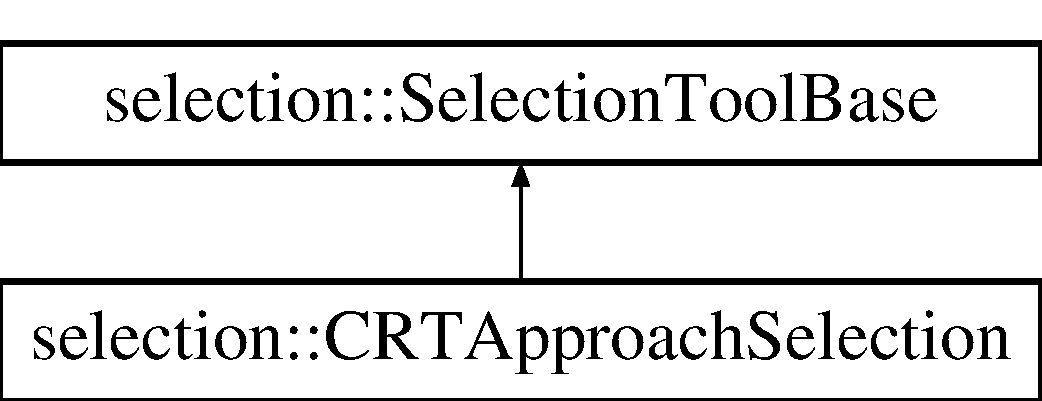
\includegraphics[height=2.000000cm]{classselection_1_1CRTApproachSelection}
\end{center}
\end{figure}
\subsection*{Public Member Functions}
\begin{DoxyCompactItemize}
\item 
\hyperlink{classselection_1_1CRTApproachSelection_ae8b705a69ee56ed6bafb37528344be85}{C\+R\+T\+Approach\+Selection} (const fhicl\+::\+Parameter\+Set \&pset)
\begin{DoxyCompactList}\small\item\em Constructor. \end{DoxyCompactList}\item 
\hyperlink{classselection_1_1CRTApproachSelection_a1ea085fa9ab18fdecbb863a25cea5eb1}{$\sim$\+C\+R\+T\+Approach\+Selection} ()\hypertarget{classselection_1_1CRTApproachSelection_a1ea085fa9ab18fdecbb863a25cea5eb1}{}\label{classselection_1_1CRTApproachSelection_a1ea085fa9ab18fdecbb863a25cea5eb1}

\begin{DoxyCompactList}\small\item\em Destructor. \end{DoxyCompactList}\item 
void \hyperlink{classselection_1_1CRTApproachSelection_a95cea2d1bd14aa512b6d4c04059d5711}{configure} (fhicl\+::\+Parameter\+Set const \&pset)
\item 
bool \hyperlink{classselection_1_1CRTApproachSelection_a9dffc74d919ac0586d57c1de740f4ce9}{select\+Event} (art\+::\+Event const \&e, const std\+::vector$<$ Proxy\+Pfp\+Elem\+\_\+t $>$ \&pfp\+\_\+pxy\+\_\+v)
\begin{DoxyCompactList}\small\item\em Selection function. \end{DoxyCompactList}\item 
void \hyperlink{classselection_1_1CRTApproachSelection_aa60ae2b3ee3f7776a3c35ed2a6aa8bea}{set\+Branches} (T\+Tree $\ast$\+\_\+tree)\hypertarget{classselection_1_1CRTApproachSelection_aa60ae2b3ee3f7776a3c35ed2a6aa8bea}{}\label{classselection_1_1CRTApproachSelection_aa60ae2b3ee3f7776a3c35ed2a6aa8bea}

\begin{DoxyCompactList}\small\item\em set branches for T\+Tree \end{DoxyCompactList}\item 
void \hyperlink{classselection_1_1CRTApproachSelection_a73491b9748240f8d5185482fe5e1d6a9}{reset\+T\+Tree} (T\+Tree $\ast$\+\_\+tree)\hypertarget{classselection_1_1CRTApproachSelection_a73491b9748240f8d5185482fe5e1d6a9}{}\label{classselection_1_1CRTApproachSelection_a73491b9748240f8d5185482fe5e1d6a9}

\begin{DoxyCompactList}\small\item\em reset ttree branches \end{DoxyCompactList}\end{DoxyCompactItemize}
\subsection*{Private Member Functions}
\begin{DoxyCompactItemize}
\item 
double {\bfseries Point2\+Point\+Distance} (const T\+Vector3 \&nuvtx, T\+Vector3 \&tagged\+Track\+Spt)\hypertarget{classselection_1_1CRTApproachSelection_a4d3cc00b6333fbdd173aed916aadb9aa}{}\label{classselection_1_1CRTApproachSelection_a4d3cc00b6333fbdd173aed916aadb9aa}

\item 
void {\bfseries Reset} ()\hypertarget{classselection_1_1CRTApproachSelection_a6a2239444e404fa929032056dddedaa7}{}\label{classselection_1_1CRTApproachSelection_a6a2239444e404fa929032056dddedaa7}

\end{DoxyCompactItemize}
\subsection*{Private Attributes}
\begin{DoxyCompactItemize}
\item 
std\+::string {\bfseries f\+Track\+Assn\+Module\+Label}\hypertarget{classselection_1_1CRTApproachSelection_a15f0ad93dde8949a296fec606099594b}{}\label{classselection_1_1CRTApproachSelection_a15f0ad93dde8949a296fec606099594b}

\item 
T\+Random3 {\bfseries rand}\hypertarget{classselection_1_1CRTApproachSelection_afdbe91721ed1cc7df5b6bcbbe839bbdd}{}\label{classselection_1_1CRTApproachSelection_afdbe91721ed1cc7df5b6bcbbe839bbdd}

\item 
Double\+\_\+t {\bfseries fid\+Vol\+MinX} = 0\hypertarget{classselection_1_1CRTApproachSelection_aa4830500d72bfd15435847dd4a1d9ac9}{}\label{classselection_1_1CRTApproachSelection_aa4830500d72bfd15435847dd4a1d9ac9}

\item 
Double\+\_\+t {\bfseries fid\+Vol\+MaxX} = 256\hypertarget{classselection_1_1CRTApproachSelection_aaedb924b21819ac956c11a3a165cfb78}{}\label{classselection_1_1CRTApproachSelection_aaedb924b21819ac956c11a3a165cfb78}

\item 
Double\+\_\+t {\bfseries fid\+Vol\+MinY} = -\/116\hypertarget{classselection_1_1CRTApproachSelection_a2e6f8ae276911170aa191edddfa5bfd7}{}\label{classselection_1_1CRTApproachSelection_a2e6f8ae276911170aa191edddfa5bfd7}

\item 
Double\+\_\+t {\bfseries fid\+Vol\+MaxY} = 116\hypertarget{classselection_1_1CRTApproachSelection_a900fe383fbffc1ebdb1cef1037c75b9b}{}\label{classselection_1_1CRTApproachSelection_a900fe383fbffc1ebdb1cef1037c75b9b}

\item 
Double\+\_\+t {\bfseries fid\+Vol\+MinZ} = 0\hypertarget{classselection_1_1CRTApproachSelection_a1306cd9d8e64fd078546195c82cb1da8}{}\label{classselection_1_1CRTApproachSelection_a1306cd9d8e64fd078546195c82cb1da8}

\item 
Double\+\_\+t {\bfseries fid\+Vol\+MaxZ} = 1030\hypertarget{classselection_1_1CRTApproachSelection_a41141e3a61edb8cd43f4fdbb47b99085}{}\label{classselection_1_1CRTApproachSelection_a41141e3a61edb8cd43f4fdbb47b99085}

\item 
int {\bfseries \+\_\+n\+Assn\+Cosmics}\hypertarget{classselection_1_1CRTApproachSelection_a4df8d6194d6c4cf796fae4b95460cd9a}{}\label{classselection_1_1CRTApproachSelection_a4df8d6194d6c4cf796fae4b95460cd9a}

\item 
Double\+\_\+t {\bfseries \+\_\+t0\+Cosm\+\_\+v} \mbox{[}k\+Max\+Cosm\mbox{]}\hypertarget{classselection_1_1CRTApproachSelection_a49116ca907aaa2d00a95da2ed52f1236}{}\label{classselection_1_1CRTApproachSelection_a49116ca907aaa2d00a95da2ed52f1236}

\item 
Double\+\_\+t {\bfseries \+\_\+t0times\+V\+Cosm\+\_\+v} \mbox{[}k\+Max\+Cosm\mbox{]}\hypertarget{classselection_1_1CRTApproachSelection_a941e9f159b6047b5d44a9804a1478d30}{}\label{classselection_1_1CRTApproachSelection_a941e9f159b6047b5d44a9804a1478d30}

\item 
Double\+\_\+t {\bfseries \+\_\+x\+Start\+Cosm\+\_\+v} \mbox{[}k\+Max\+Cosm\mbox{]}\hypertarget{classselection_1_1CRTApproachSelection_a189f83134073d683c1d5c7082508d6ad}{}\label{classselection_1_1CRTApproachSelection_a189f83134073d683c1d5c7082508d6ad}

\item 
Double\+\_\+t {\bfseries \+\_\+y\+Start\+Cosm\+\_\+v} \mbox{[}k\+Max\+Cosm\mbox{]}\hypertarget{classselection_1_1CRTApproachSelection_a471d3c4a511c7ddd24051ee1f25e0e53}{}\label{classselection_1_1CRTApproachSelection_a471d3c4a511c7ddd24051ee1f25e0e53}

\item 
Double\+\_\+t {\bfseries \+\_\+z\+Start\+Cosm\+\_\+v} \mbox{[}k\+Max\+Cosm\mbox{]}\hypertarget{classselection_1_1CRTApproachSelection_ac7791dd93144935b887d474bee62be04}{}\label{classselection_1_1CRTApproachSelection_ac7791dd93144935b887d474bee62be04}

\item 
Double\+\_\+t {\bfseries \+\_\+x\+End\+Cosm\+\_\+v} \mbox{[}k\+Max\+Cosm\mbox{]}\hypertarget{classselection_1_1CRTApproachSelection_a367f33de2c7b2e47bbecca1d110227ea}{}\label{classselection_1_1CRTApproachSelection_a367f33de2c7b2e47bbecca1d110227ea}

\item 
Double\+\_\+t {\bfseries \+\_\+y\+End\+Cosm\+\_\+v} \mbox{[}k\+Max\+Cosm\mbox{]}\hypertarget{classselection_1_1CRTApproachSelection_a5bb5ca3e2da1a35bcdc619b6151337b9}{}\label{classselection_1_1CRTApproachSelection_a5bb5ca3e2da1a35bcdc619b6151337b9}

\item 
Double\+\_\+t {\bfseries \+\_\+z\+End\+Cosm\+\_\+v} \mbox{[}k\+Max\+Cosm\mbox{]}\hypertarget{classselection_1_1CRTApproachSelection_a72d234158d1a41f31b2cdf392b783a36}{}\label{classselection_1_1CRTApproachSelection_a72d234158d1a41f31b2cdf392b783a36}

\item 
Double\+\_\+t {\bfseries \+\_\+reco\+Nu\+\_\+vtx\+\_\+x}\hypertarget{classselection_1_1CRTApproachSelection_a056d8f8b317520117e9c79a1ad1a2079}{}\label{classselection_1_1CRTApproachSelection_a056d8f8b317520117e9c79a1ad1a2079}

\item 
Double\+\_\+t {\bfseries \+\_\+reco\+Nu\+\_\+vtx\+\_\+y}\hypertarget{classselection_1_1CRTApproachSelection_a719f0440e7e5ea502ceac242c1fe7c29}{}\label{classselection_1_1CRTApproachSelection_a719f0440e7e5ea502ceac242c1fe7c29}

\item 
Double\+\_\+t {\bfseries \+\_\+reco\+Nu\+\_\+vtx\+\_\+z}\hypertarget{classselection_1_1CRTApproachSelection_a63a5d13d762d76da5331aa2223e480e0}{}\label{classselection_1_1CRTApproachSelection_a63a5d13d762d76da5331aa2223e480e0}

\item 
Double\+\_\+t {\bfseries \+\_\+t0\+\_\+nu\+\_\+cosmic}\hypertarget{classselection_1_1CRTApproachSelection_a29b5f9f8d30390e163e3c3bfd60edd43}{}\label{classselection_1_1CRTApproachSelection_a29b5f9f8d30390e163e3c3bfd60edd43}

\item 
Double\+\_\+t {\bfseries \+\_\+nu\+\_\+cosmic\+\_\+x}\hypertarget{classselection_1_1CRTApproachSelection_a310ec7069e860d855f02412d1fe3b799}{}\label{classselection_1_1CRTApproachSelection_a310ec7069e860d855f02412d1fe3b799}

\item 
Double\+\_\+t {\bfseries \+\_\+nu\+\_\+cosmic\+\_\+y}\hypertarget{classselection_1_1CRTApproachSelection_a103e7f76598ba38aa819187496e8d951}{}\label{classselection_1_1CRTApproachSelection_a103e7f76598ba38aa819187496e8d951}

\item 
Double\+\_\+t {\bfseries \+\_\+nu\+\_\+cosmic\+\_\+z}\hypertarget{classselection_1_1CRTApproachSelection_a7ab5907c21cc947cd59e1de07acbc203}{}\label{classselection_1_1CRTApproachSelection_a7ab5907c21cc947cd59e1de07acbc203}

\item 
Double\+\_\+t {\bfseries \+\_\+nu\+\_\+cosmic\+\_\+\+Length}\hypertarget{classselection_1_1CRTApproachSelection_abff8ae0c55ebdf10c713580d17f46663}{}\label{classselection_1_1CRTApproachSelection_abff8ae0c55ebdf10c713580d17f46663}

\item 
Double\+\_\+t {\bfseries \+\_\+nu\+\_\+cosmic\+\_\+\+Start\+\_\+x}\hypertarget{classselection_1_1CRTApproachSelection_a58a7fe3ea0490d6dad5b4ba89b5faf90}{}\label{classselection_1_1CRTApproachSelection_a58a7fe3ea0490d6dad5b4ba89b5faf90}

\item 
Double\+\_\+t {\bfseries \+\_\+nu\+\_\+cosmic\+\_\+\+Start\+\_\+y}\hypertarget{classselection_1_1CRTApproachSelection_a556dae3cb373081bf9bda316bc6c058a}{}\label{classselection_1_1CRTApproachSelection_a556dae3cb373081bf9bda316bc6c058a}

\item 
Double\+\_\+t {\bfseries \+\_\+nu\+\_\+cosmic\+\_\+\+Start\+\_\+z}\hypertarget{classselection_1_1CRTApproachSelection_ae990bd5d3c7f80ddb66717ae2e0178d3}{}\label{classselection_1_1CRTApproachSelection_ae990bd5d3c7f80ddb66717ae2e0178d3}

\item 
Double\+\_\+t {\bfseries \+\_\+nu\+\_\+cosmic\+\_\+\+End\+\_\+x}\hypertarget{classselection_1_1CRTApproachSelection_aebaf3d874866dd5de87b3650ed8ce5b1}{}\label{classselection_1_1CRTApproachSelection_aebaf3d874866dd5de87b3650ed8ce5b1}

\item 
Double\+\_\+t {\bfseries \+\_\+nu\+\_\+cosmic\+\_\+\+End\+\_\+y}\hypertarget{classselection_1_1CRTApproachSelection_ac28483dccfc975f5de3639e4d7e9ca55}{}\label{classselection_1_1CRTApproachSelection_ac28483dccfc975f5de3639e4d7e9ca55}

\item 
Double\+\_\+t {\bfseries \+\_\+nu\+\_\+cosmic\+\_\+\+End\+\_\+z}\hypertarget{classselection_1_1CRTApproachSelection_a65d48e1480cdbdf20f1407626915114c}{}\label{classselection_1_1CRTApproachSelection_a65d48e1480cdbdf20f1407626915114c}

\item 
Double\+\_\+t {\bfseries \+\_\+nu\+\_\+cosmic\+\_\+\+Track\+ID}\hypertarget{classselection_1_1CRTApproachSelection_a9036f20b627952fae88de7737284ae7c}{}\label{classselection_1_1CRTApproachSelection_a9036f20b627952fae88de7737284ae7c}

\item 
Double\+\_\+t {\bfseries \+\_\+closest\+Nu\+Cosmic\+Dist} = 999999999.\hypertarget{classselection_1_1CRTApproachSelection_a747913403b82418024381ce20dfd7c83}{}\label{classselection_1_1CRTApproachSelection_a747913403b82418024381ce20dfd7c83}

\item 
Double\+\_\+t {\bfseries \+\_\+rand\+\_\+vtx\+\_\+x}\hypertarget{classselection_1_1CRTApproachSelection_a378772ebaed8243d7ee8a479442873c4}{}\label{classselection_1_1CRTApproachSelection_a378772ebaed8243d7ee8a479442873c4}

\item 
Double\+\_\+t {\bfseries \+\_\+rand\+\_\+vtx\+\_\+y}\hypertarget{classselection_1_1CRTApproachSelection_a03b5a1dcd544a48e87c18a5677d830ca}{}\label{classselection_1_1CRTApproachSelection_a03b5a1dcd544a48e87c18a5677d830ca}

\item 
Double\+\_\+t {\bfseries \+\_\+rand\+\_\+vtx\+\_\+z}\hypertarget{classselection_1_1CRTApproachSelection_ab219e9bc7b7e254a8e41cf1f44de8dc6}{}\label{classselection_1_1CRTApproachSelection_ab219e9bc7b7e254a8e41cf1f44de8dc6}

\item 
Double\+\_\+t {\bfseries \+\_\+t0\+\_\+rand\+\_\+cosmic}\hypertarget{classselection_1_1CRTApproachSelection_a1ad8fe8bd1316510ec6561f2f1b516f2}{}\label{classselection_1_1CRTApproachSelection_a1ad8fe8bd1316510ec6561f2f1b516f2}

\item 
Double\+\_\+t {\bfseries \+\_\+rand\+\_\+cosmic\+\_\+x}\hypertarget{classselection_1_1CRTApproachSelection_a3cc8360576cea5a870f5f34a176cabfc}{}\label{classselection_1_1CRTApproachSelection_a3cc8360576cea5a870f5f34a176cabfc}

\item 
Double\+\_\+t {\bfseries \+\_\+rand\+\_\+cosmic\+\_\+y}\hypertarget{classselection_1_1CRTApproachSelection_ac2fe4c06766a03e651f408f834c38244}{}\label{classselection_1_1CRTApproachSelection_ac2fe4c06766a03e651f408f834c38244}

\item 
Double\+\_\+t {\bfseries \+\_\+rand\+\_\+cosmic\+\_\+z}\hypertarget{classselection_1_1CRTApproachSelection_a6d9f1f606c935827b09fe727a72ce673}{}\label{classselection_1_1CRTApproachSelection_a6d9f1f606c935827b09fe727a72ce673}

\item 
Double\+\_\+t {\bfseries \+\_\+rand\+\_\+cosmic\+\_\+\+Length}\hypertarget{classselection_1_1CRTApproachSelection_ae78c617886be32335dff2a84a3fb4909}{}\label{classselection_1_1CRTApproachSelection_ae78c617886be32335dff2a84a3fb4909}

\item 
Double\+\_\+t {\bfseries \+\_\+rand\+\_\+cosmic\+\_\+\+Start\+\_\+x}\hypertarget{classselection_1_1CRTApproachSelection_af583dfbb51a0680410b6c3bb7ff72a1b}{}\label{classselection_1_1CRTApproachSelection_af583dfbb51a0680410b6c3bb7ff72a1b}

\item 
Double\+\_\+t {\bfseries \+\_\+rand\+\_\+cosmic\+\_\+\+Start\+\_\+y}\hypertarget{classselection_1_1CRTApproachSelection_a0a6bbbf9b57616f04f5e9e722542ebd1}{}\label{classselection_1_1CRTApproachSelection_a0a6bbbf9b57616f04f5e9e722542ebd1}

\item 
Double\+\_\+t {\bfseries \+\_\+rand\+\_\+cosmic\+\_\+\+Start\+\_\+z}\hypertarget{classselection_1_1CRTApproachSelection_ac01829671455b1c595e944b00b2cfde4}{}\label{classselection_1_1CRTApproachSelection_ac01829671455b1c595e944b00b2cfde4}

\item 
Double\+\_\+t {\bfseries \+\_\+rand\+\_\+cosmic\+\_\+\+End\+\_\+x}\hypertarget{classselection_1_1CRTApproachSelection_abc2bb317bd856e749c2395407b4293f5}{}\label{classselection_1_1CRTApproachSelection_abc2bb317bd856e749c2395407b4293f5}

\item 
Double\+\_\+t {\bfseries \+\_\+rand\+\_\+cosmic\+\_\+\+End\+\_\+y}\hypertarget{classselection_1_1CRTApproachSelection_afe50ea2e4b51e72832e952836989c833}{}\label{classselection_1_1CRTApproachSelection_afe50ea2e4b51e72832e952836989c833}

\item 
Double\+\_\+t {\bfseries \+\_\+rand\+\_\+cosmic\+\_\+\+End\+\_\+z}\hypertarget{classselection_1_1CRTApproachSelection_aa7e0dd80764787acb3a4201f17f731eb}{}\label{classselection_1_1CRTApproachSelection_aa7e0dd80764787acb3a4201f17f731eb}

\item 
Double\+\_\+t {\bfseries \+\_\+rand\+\_\+cosmic\+\_\+\+Track\+ID}\hypertarget{classselection_1_1CRTApproachSelection_ad0c733ea5c72da5dadc0305ffc8c76d0}{}\label{classselection_1_1CRTApproachSelection_ad0c733ea5c72da5dadc0305ffc8c76d0}

\item 
Double\+\_\+t {\bfseries \+\_\+closest\+Rand\+Cosmic\+Dist} = 999999999.\hypertarget{classselection_1_1CRTApproachSelection_af6412c820768d9db1ee2ad8c699f0d4f}{}\label{classselection_1_1CRTApproachSelection_af6412c820768d9db1ee2ad8c699f0d4f}

\end{DoxyCompactItemize}
\subsection*{Additional Inherited Members}


\subsection{Constructor \& Destructor Documentation}
\index{selection\+::\+C\+R\+T\+Approach\+Selection@{selection\+::\+C\+R\+T\+Approach\+Selection}!C\+R\+T\+Approach\+Selection@{C\+R\+T\+Approach\+Selection}}
\index{C\+R\+T\+Approach\+Selection@{C\+R\+T\+Approach\+Selection}!selection\+::\+C\+R\+T\+Approach\+Selection@{selection\+::\+C\+R\+T\+Approach\+Selection}}
\subsubsection[{\texorpdfstring{C\+R\+T\+Approach\+Selection(const fhicl\+::\+Parameter\+Set \&pset)}{CRTApproachSelection(const fhicl::ParameterSet &pset)}}]{\setlength{\rightskip}{0pt plus 5cm}selection\+::\+C\+R\+T\+Approach\+Selection\+::\+C\+R\+T\+Approach\+Selection (
\begin{DoxyParamCaption}
\item[{const fhicl\+::\+Parameter\+Set \&}]{pset}
\end{DoxyParamCaption}
)}\hypertarget{classselection_1_1CRTApproachSelection_ae8b705a69ee56ed6bafb37528344be85}{}\label{classselection_1_1CRTApproachSelection_ae8b705a69ee56ed6bafb37528344be85}


Constructor. 


\begin{DoxyParams}{Parameters}
{\em pset} & Constructor.\\
\hline
\end{DoxyParams}
Arguments\+:

pset -\/ Fcl parameters. 

\subsection{Member Function Documentation}
\index{selection\+::\+C\+R\+T\+Approach\+Selection@{selection\+::\+C\+R\+T\+Approach\+Selection}!configure@{configure}}
\index{configure@{configure}!selection\+::\+C\+R\+T\+Approach\+Selection@{selection\+::\+C\+R\+T\+Approach\+Selection}}
\subsubsection[{\texorpdfstring{configure(fhicl\+::\+Parameter\+Set const \&pset)}{configure(fhicl::ParameterSet const &pset)}}]{\setlength{\rightskip}{0pt plus 5cm}void selection\+::\+C\+R\+T\+Approach\+Selection\+::configure (
\begin{DoxyParamCaption}
\item[{fhicl\+::\+Parameter\+Set const \&}]{pset}
\end{DoxyParamCaption}
)}\hypertarget{classselection_1_1CRTApproachSelection_a95cea2d1bd14aa512b6d4c04059d5711}{}\label{classselection_1_1CRTApproachSelection_a95cea2d1bd14aa512b6d4c04059d5711}
Reconfigure method.

Arguments\+:

pset -\/ Fcl parameter set. \index{selection\+::\+C\+R\+T\+Approach\+Selection@{selection\+::\+C\+R\+T\+Approach\+Selection}!select\+Event@{select\+Event}}
\index{select\+Event@{select\+Event}!selection\+::\+C\+R\+T\+Approach\+Selection@{selection\+::\+C\+R\+T\+Approach\+Selection}}
\subsubsection[{\texorpdfstring{select\+Event(art\+::\+Event const \&e, const std\+::vector$<$ Proxy\+Pfp\+Elem\+\_\+t $>$ \&pfp\+\_\+pxy\+\_\+v)}{selectEvent(art::Event const &e, const std::vector< ProxyPfpElem_t > &pfp_pxy_v)}}]{\setlength{\rightskip}{0pt plus 5cm}bool selection\+::\+C\+R\+T\+Approach\+Selection\+::select\+Event (
\begin{DoxyParamCaption}
\item[{art\+::\+Event const \&}]{e, }
\item[{const std\+::vector$<$ Proxy\+Pfp\+Elem\+\_\+t $>$ \&}]{pfp\+\_\+pxy\+\_\+v}
\end{DoxyParamCaption}
)\hspace{0.3cm}{\ttfamily [virtual]}}\hypertarget{classselection_1_1CRTApproachSelection_a9dffc74d919ac0586d57c1de740f4ce9}{}\label{classselection_1_1CRTApproachSelection_a9dffc74d919ac0586d57c1de740f4ce9}


Selection function. 

select\+Event

Arguments\+:

art\+::\+Event slice track pointer vector slice shower pointer vector 

Implements \hyperlink{classselection_1_1SelectionToolBase_ab63818dac49b43418fe9eb3b8cd98c9c}{selection\+::\+Selection\+Tool\+Base}.



The documentation for this class was generated from the following file\+:\begin{DoxyCompactItemize}
\item 
/home/travis/build/ubneutrinos/searchingfornues/\+Selection/\+Selection\+Tools/C\+R\+T\+Approach\+Selection\+\_\+tool.\+cc\end{DoxyCompactItemize}

\hypertarget{classanalysis_1_1DefaultAnalysis}{}\section{analysis\+:\+:Default\+Analysis Class Reference}
\label{classanalysis_1_1DefaultAnalysis}\index{analysis\+::\+Default\+Analysis@{analysis\+::\+Default\+Analysis}}
Inheritance diagram for analysis\+:\+:Default\+Analysis\+:\begin{figure}[H]
\begin{center}
\leavevmode
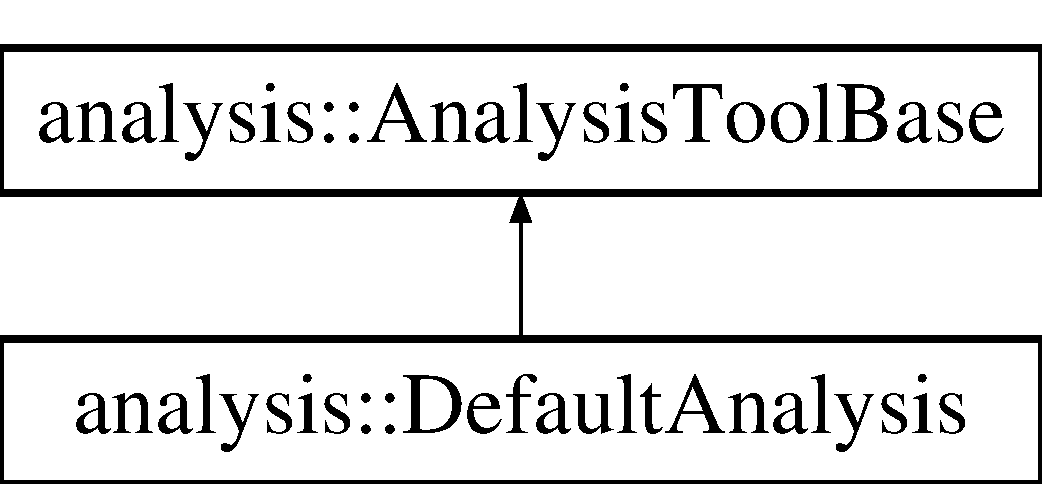
\includegraphics[height=2.000000cm]{classanalysis_1_1DefaultAnalysis}
\end{center}
\end{figure}
\subsection*{Public Member Functions}
\begin{DoxyCompactItemize}
\item 
\hyperlink{classanalysis_1_1DefaultAnalysis_a857349701c91ee06075ea01c5edc15b6}{Default\+Analysis} (const fhicl\+::\+Parameter\+Set \&pset)
\begin{DoxyCompactList}\small\item\em Constructor. \end{DoxyCompactList}\item 
\hyperlink{classanalysis_1_1DefaultAnalysis_ad4be6c0a18f97e1d02a5c1e905ac5786}{$\sim$\+Default\+Analysis} ()\hypertarget{classanalysis_1_1DefaultAnalysis_ad4be6c0a18f97e1d02a5c1e905ac5786}{}\label{classanalysis_1_1DefaultAnalysis_ad4be6c0a18f97e1d02a5c1e905ac5786}

\begin{DoxyCompactList}\small\item\em Destructor. \end{DoxyCompactList}\item 
void \hyperlink{classanalysis_1_1DefaultAnalysis_a475f62ff6b6dae44bb4f3c917f0970de}{configure} (fhicl\+::\+Parameter\+Set const \&pset)
\item 
void \hyperlink{classanalysis_1_1DefaultAnalysis_a0cf6d593602ba67c23fae67ca7989c10}{analyze\+Event} (art\+::\+Event const \&e, bool f\+Data) override
\begin{DoxyCompactList}\small\item\em Analysis function. \end{DoxyCompactList}\item 
void \hyperlink{classanalysis_1_1DefaultAnalysis_ad676faeeb49900efb0c9a615a60d179c}{analyze\+Slice} (art\+::\+Event const \&e, std\+::vector$<$ Proxy\+Pfp\+Elem\+\_\+t $>$ \&slice\+\_\+pfp\+\_\+v, bool f\+Data, bool selected) override\hypertarget{classanalysis_1_1DefaultAnalysis_ad676faeeb49900efb0c9a615a60d179c}{}\label{classanalysis_1_1DefaultAnalysis_ad676faeeb49900efb0c9a615a60d179c}

\begin{DoxyCompactList}\small\item\em Analyze slice. \end{DoxyCompactList}\item 
void \hyperlink{classanalysis_1_1DefaultAnalysis_a5d973c6b88477330f6b744f3c9c60dd6}{Save\+Truth} (art\+::\+Event const \&e)\hypertarget{classanalysis_1_1DefaultAnalysis_a5d973c6b88477330f6b744f3c9c60dd6}{}\label{classanalysis_1_1DefaultAnalysis_a5d973c6b88477330f6b744f3c9c60dd6}

\begin{DoxyCompactList}\small\item\em Save truth info for event associated to neutrino. \end{DoxyCompactList}\item 
void \hyperlink{classanalysis_1_1DefaultAnalysis_a95b4abd17b0d77b436f5f6ae43e641c7}{set\+Branches} (T\+Tree $\ast$\+\_\+tree) override\hypertarget{classanalysis_1_1DefaultAnalysis_a95b4abd17b0d77b436f5f6ae43e641c7}{}\label{classanalysis_1_1DefaultAnalysis_a95b4abd17b0d77b436f5f6ae43e641c7}

\begin{DoxyCompactList}\small\item\em set branches for T\+Tree \end{DoxyCompactList}\item 
void \hyperlink{classanalysis_1_1DefaultAnalysis_a732ca63923ff91a3928dc437c2e04adf}{reset\+T\+Tree} (T\+Tree $\ast$\+\_\+tree) override\hypertarget{classanalysis_1_1DefaultAnalysis_a732ca63923ff91a3928dc437c2e04adf}{}\label{classanalysis_1_1DefaultAnalysis_a732ca63923ff91a3928dc437c2e04adf}

\begin{DoxyCompactList}\small\item\em reset ttree branches \end{DoxyCompactList}\end{DoxyCompactItemize}
\subsection*{Private Member Functions}
\begin{DoxyCompactItemize}
\item 
void \hyperlink{classanalysis_1_1DefaultAnalysis_a248e4a44368e7c8a632242fa7e171ade}{Apply\+S\+C\+E\+Correction} (const float \&vtx\+\_\+x, const float \&vtx\+\_\+y, const float \&vtx\+\_\+z, float \&sce\+\_\+x, float \&sce\+\_\+y, float \&sce\+\_\+z)\hypertarget{classanalysis_1_1DefaultAnalysis_a248e4a44368e7c8a632242fa7e171ade}{}\label{classanalysis_1_1DefaultAnalysis_a248e4a44368e7c8a632242fa7e171ade}

\begin{DoxyCompactList}\small\item\em apply S\+CE corections from reconstruction maps \end{DoxyCompactList}\item 
bool \hyperlink{classanalysis_1_1DefaultAnalysis_a51efe899f0117f479c9f833663c7111f}{is\+Fiducial} (const double x\mbox{[}3\mbox{]}) const 
\begin{DoxyCompactList}\small\item\em Determine if the specified point is in the fiducial volume Not recommended, no array size checking is done. \end{DoxyCompactList}\end{DoxyCompactItemize}
\subsection*{Private Attributes}
\begin{DoxyCompactItemize}
\item 
T\+Particle\+P\+DG $\ast$ {\bfseries proton} = T\+Database\+P\+D\+G\+::\+Instance()-\/$>$Get\+Particle(2212)\hypertarget{classanalysis_1_1DefaultAnalysis_a93050a6176a0497f73a16db74a686c53}{}\label{classanalysis_1_1DefaultAnalysis_a93050a6176a0497f73a16db74a686c53}

\item 
T\+Particle\+P\+DG $\ast$ {\bfseries neutron} = T\+Database\+P\+D\+G\+::\+Instance()-\/$>$Get\+Particle(2112)\hypertarget{classanalysis_1_1DefaultAnalysis_a82cdc332e30f34fd12ec5493808cc28c}{}\label{classanalysis_1_1DefaultAnalysis_a82cdc332e30f34fd12ec5493808cc28c}

\item 
T\+Particle\+P\+DG $\ast$ {\bfseries electron} = T\+Database\+P\+D\+G\+::\+Instance()-\/$>$Get\+Particle(11)\hypertarget{classanalysis_1_1DefaultAnalysis_a1089802dee9a5e84c00e7e007dde2746}{}\label{classanalysis_1_1DefaultAnalysis_a1089802dee9a5e84c00e7e007dde2746}

\item 
T\+Particle\+P\+DG $\ast$ {\bfseries muon} = T\+Database\+P\+D\+G\+::\+Instance()-\/$>$Get\+Particle(13)\hypertarget{classanalysis_1_1DefaultAnalysis_a497f1c0211f19df2985b622a4c536933}{}\label{classanalysis_1_1DefaultAnalysis_a497f1c0211f19df2985b622a4c536933}

\item 
T\+Particle\+P\+DG $\ast$ {\bfseries pion} = T\+Database\+P\+D\+G\+::\+Instance()-\/$>$Get\+Particle(211)\hypertarget{classanalysis_1_1DefaultAnalysis_a8eefb85a44d77ee187587fb687edda77}{}\label{classanalysis_1_1DefaultAnalysis_a8eefb85a44d77ee187587fb687edda77}

\item 
T\+Particle\+P\+DG $\ast$ {\bfseries pi0} = T\+Database\+P\+D\+G\+::\+Instance()-\/$>$Get\+Particle(111)\hypertarget{classanalysis_1_1DefaultAnalysis_a01ede37c4c112f9fd8e4bd4e0b33d123}{}\label{classanalysis_1_1DefaultAnalysis_a01ede37c4c112f9fd8e4bd4e0b33d123}

\item 
T\+Particle\+P\+DG $\ast$ {\bfseries electron\+\_\+neutrino} = T\+Database\+P\+D\+G\+::\+Instance()-\/$>$Get\+Particle(12)\hypertarget{classanalysis_1_1DefaultAnalysis_adba116e53c02e5f2de721bc7a7eb909e}{}\label{classanalysis_1_1DefaultAnalysis_adba116e53c02e5f2de721bc7a7eb909e}

\item 
T\+Particle\+P\+DG $\ast$ {\bfseries muon\+\_\+neutrino} = T\+Database\+P\+D\+G\+::\+Instance()-\/$>$Get\+Particle(14)\hypertarget{classanalysis_1_1DefaultAnalysis_a0e76c2baabff12b0a3f19aa54c54a59d}{}\label{classanalysis_1_1DefaultAnalysis_a0e76c2baabff12b0a3f19aa54c54a59d}

\item 
art\+::\+Input\+Tag {\bfseries f\+C\+R\+T\+Vetoproducer}\hypertarget{classanalysis_1_1DefaultAnalysis_aba3c76b59d2a5b2e24f50b2868c4c045}{}\label{classanalysis_1_1DefaultAnalysis_aba3c76b59d2a5b2e24f50b2868c4c045}

\item 
art\+::\+Input\+Tag {\bfseries f\+C\+L\+Sproducer}\hypertarget{classanalysis_1_1DefaultAnalysis_ae4cd0c3f1d34676303c2bf78512b1033}{}\label{classanalysis_1_1DefaultAnalysis_ae4cd0c3f1d34676303c2bf78512b1033}

\item 
art\+::\+Input\+Tag {\bfseries f\+M\+C\+Tproducer}\hypertarget{classanalysis_1_1DefaultAnalysis_a5a9b0c6d9996f8c7198158b3f36acd67}{}\label{classanalysis_1_1DefaultAnalysis_a5a9b0c6d9996f8c7198158b3f36acd67}

\item 
art\+::\+Input\+Tag {\bfseries f\+M\+C\+Pproducer}\hypertarget{classanalysis_1_1DefaultAnalysis_ad10d6b02fc6fcd46a25c30877f1fb634}{}\label{classanalysis_1_1DefaultAnalysis_ad10d6b02fc6fcd46a25c30877f1fb634}

\item 
art\+::\+Input\+Tag {\bfseries f\+Backtrack\+Tag}\hypertarget{classanalysis_1_1DefaultAnalysis_a8dab9b6e3afeeb11bf7baf043daa5ecd}{}\label{classanalysis_1_1DefaultAnalysis_a8dab9b6e3afeeb11bf7baf043daa5ecd}

\item 
art\+::\+Input\+Tag {\bfseries f\+Hproducer}\hypertarget{classanalysis_1_1DefaultAnalysis_a4fbfc54f63dec8d38301ad853ed9f719}{}\label{classanalysis_1_1DefaultAnalysis_a4fbfc54f63dec8d38301ad853ed9f719}

\item 
art\+::\+Input\+Tag {\bfseries f\+M\+C\+Rproducer}\hypertarget{classanalysis_1_1DefaultAnalysis_abf7821b91f9c87b40cbefa49824bebe7}{}\label{classanalysis_1_1DefaultAnalysis_abf7821b91f9c87b40cbefa49824bebe7}

\item 
art\+::\+Input\+Tag {\bfseries f\+S\+L\+Cproducer}\hypertarget{classanalysis_1_1DefaultAnalysis_ac3aef1da86526ce278fc67a56a73d759}{}\label{classanalysis_1_1DefaultAnalysis_ac3aef1da86526ce278fc67a56a73d759}

\item 
float \hyperlink{classanalysis_1_1DefaultAnalysis_aba718fab9e0072c6a046b9f9aa3670bf}{f\+Trk\+Shr\+Score}
\item 
float {\bfseries f\+Fidvol\+Xstart}\hypertarget{classanalysis_1_1DefaultAnalysis_a71ab40d790e7449fd11a07daa6881dfb}{}\label{classanalysis_1_1DefaultAnalysis_a71ab40d790e7449fd11a07daa6881dfb}

\item 
float {\bfseries f\+Fidvol\+Xend}\hypertarget{classanalysis_1_1DefaultAnalysis_a652ed60c4510fdb1bf2e4f8fe472fcd0}{}\label{classanalysis_1_1DefaultAnalysis_a652ed60c4510fdb1bf2e4f8fe472fcd0}

\item 
float {\bfseries f\+Fidvol\+Ystart}\hypertarget{classanalysis_1_1DefaultAnalysis_acc3b004be143ee4128dd940e099a5b21}{}\label{classanalysis_1_1DefaultAnalysis_acc3b004be143ee4128dd940e099a5b21}

\item 
float {\bfseries f\+Fidvol\+Yend}\hypertarget{classanalysis_1_1DefaultAnalysis_a7aac9ffed4983dfeb62c3d31c6029144}{}\label{classanalysis_1_1DefaultAnalysis_a7aac9ffed4983dfeb62c3d31c6029144}

\item 
float {\bfseries f\+Fidvol\+Zstart}\hypertarget{classanalysis_1_1DefaultAnalysis_ae5eccb9eededfcbbbc508d2e5aa97799}{}\label{classanalysis_1_1DefaultAnalysis_ae5eccb9eededfcbbbc508d2e5aa97799}

\item 
float {\bfseries f\+Fidvol\+Zend}\hypertarget{classanalysis_1_1DefaultAnalysis_ab1b95314c090f6891a698de004fd800a}{}\label{classanalysis_1_1DefaultAnalysis_ab1b95314c090f6891a698de004fd800a}

\item 
const int {\bfseries k\+\_\+nu\+\_\+e\+\_\+other} = 1\hypertarget{classanalysis_1_1DefaultAnalysis_a60df74ed4d08dee6e14779e36618f39f}{}\label{classanalysis_1_1DefaultAnalysis_a60df74ed4d08dee6e14779e36618f39f}

\item 
const int {\bfseries k\+\_\+nu\+\_\+e\+\_\+cc0pi0p} = 10\hypertarget{classanalysis_1_1DefaultAnalysis_a55005c4e1539179b318db9b8a2c4f5fe}{}\label{classanalysis_1_1DefaultAnalysis_a55005c4e1539179b318db9b8a2c4f5fe}

\item 
const int {\bfseries k\+\_\+nu\+\_\+e\+\_\+cc0pinp} = 11\hypertarget{classanalysis_1_1DefaultAnalysis_a8779a2bbc714bc263e28ed4d7cbacfc4}{}\label{classanalysis_1_1DefaultAnalysis_a8779a2bbc714bc263e28ed4d7cbacfc4}

\item 
const int {\bfseries k\+\_\+nu\+\_\+mu\+\_\+other} = 2\hypertarget{classanalysis_1_1DefaultAnalysis_a11416c43cdc46c0cd7f112a459f82e5e}{}\label{classanalysis_1_1DefaultAnalysis_a11416c43cdc46c0cd7f112a459f82e5e}

\item 
const int {\bfseries k\+\_\+nu\+\_\+mu\+\_\+pi0} = 21\hypertarget{classanalysis_1_1DefaultAnalysis_aa493279c647932c0c73a8b393450533a}{}\label{classanalysis_1_1DefaultAnalysis_aa493279c647932c0c73a8b393450533a}

\item 
const int {\bfseries k\+\_\+nc} = 3\hypertarget{classanalysis_1_1DefaultAnalysis_a5919c7e3eb507b4b1a96ac560961352a}{}\label{classanalysis_1_1DefaultAnalysis_a5919c7e3eb507b4b1a96ac560961352a}

\item 
const int {\bfseries k\+\_\+nc\+\_\+pi0} = 31\hypertarget{classanalysis_1_1DefaultAnalysis_aca2b8b9faf52c405c67d08b67cb8f9c6}{}\label{classanalysis_1_1DefaultAnalysis_aca2b8b9faf52c405c67d08b67cb8f9c6}

\item 
const int {\bfseries k\+\_\+cosmic} = 4\hypertarget{classanalysis_1_1DefaultAnalysis_ab7eb29cdf5e3f90c0402276ea97f11d8}{}\label{classanalysis_1_1DefaultAnalysis_ab7eb29cdf5e3f90c0402276ea97f11d8}

\item 
const int {\bfseries k\+\_\+outfv} = 5\hypertarget{classanalysis_1_1DefaultAnalysis_a1c78b3c26d574995ed70e76c16cfbd3c}{}\label{classanalysis_1_1DefaultAnalysis_a1c78b3c26d574995ed70e76c16cfbd3c}

\item 
const int {\bfseries k\+\_\+other} = 6\hypertarget{classanalysis_1_1DefaultAnalysis_af085b9d960ab70ebdf5d1dbc862c994c}{}\label{classanalysis_1_1DefaultAnalysis_af085b9d960ab70ebdf5d1dbc862c994c}

\item 
const int {\bfseries k\+\_\+data} = 0\hypertarget{classanalysis_1_1DefaultAnalysis_ad90304e9066f094415ce5ea119ce7139}{}\label{classanalysis_1_1DefaultAnalysis_ad90304e9066f094415ce5ea119ce7139}

\item 
float {\bfseries f\+Proton\+Threshold}\hypertarget{classanalysis_1_1DefaultAnalysis_a31cfe4d3b99c54eb1dcf637c26234df4}{}\label{classanalysis_1_1DefaultAnalysis_a31cfe4d3b99c54eb1dcf637c26234df4}

\item 
float {\bfseries f\+Pion\+Threshold}\hypertarget{classanalysis_1_1DefaultAnalysis_a611a441c3b57941607df65ec720123c2}{}\label{classanalysis_1_1DefaultAnalysis_a611a441c3b57941607df65ec720123c2}

\item 
float {\bfseries f\+Pi0\+Threshold}\hypertarget{classanalysis_1_1DefaultAnalysis_a033846ebe00f83a17785111e5b7f55a1}{}\label{classanalysis_1_1DefaultAnalysis_a033846ebe00f83a17785111e5b7f55a1}

\item 
float {\bfseries f\+Electron\+Threshold}\hypertarget{classanalysis_1_1DefaultAnalysis_a55296431f6111d81ac812be8aabcb6df}{}\label{classanalysis_1_1DefaultAnalysis_a55296431f6111d81ac812be8aabcb6df}

\item 
float {\bfseries f\+Muon\+Threshold}\hypertarget{classanalysis_1_1DefaultAnalysis_adbaf1e9b8ebd103ac8bbad82fb0127a4}{}\label{classanalysis_1_1DefaultAnalysis_adbaf1e9b8ebd103ac8bbad82fb0127a4}

\item 
int {\bfseries \+\_\+category}\hypertarget{classanalysis_1_1DefaultAnalysis_a439203d5925baa2ccdd8108618801267}{}\label{classanalysis_1_1DefaultAnalysis_a439203d5925baa2ccdd8108618801267}

\item 
float {\bfseries \+\_\+nu\+\_\+vtx\+\_\+x}\hypertarget{classanalysis_1_1DefaultAnalysis_ae74ddbcfe3d655a7a2ef2e7f51110c8b}{}\label{classanalysis_1_1DefaultAnalysis_ae74ddbcfe3d655a7a2ef2e7f51110c8b}

\item 
float {\bfseries \+\_\+nu\+\_\+vtx\+\_\+y}\hypertarget{classanalysis_1_1DefaultAnalysis_a60598c35745e81417d2fe44a7198a3cf}{}\label{classanalysis_1_1DefaultAnalysis_a60598c35745e81417d2fe44a7198a3cf}

\item 
float {\bfseries \+\_\+nu\+\_\+vtx\+\_\+z}\hypertarget{classanalysis_1_1DefaultAnalysis_a61e5383c17b136ad3c0d62c1d91d972e}{}\label{classanalysis_1_1DefaultAnalysis_a61e5383c17b136ad3c0d62c1d91d972e}

\item 
float {\bfseries \+\_\+nu\+\_\+sce\+\_\+x}\hypertarget{classanalysis_1_1DefaultAnalysis_ae15f1f173710c3763e52e8341d6d6e9b}{}\label{classanalysis_1_1DefaultAnalysis_ae15f1f173710c3763e52e8341d6d6e9b}

\item 
float {\bfseries \+\_\+nu\+\_\+sce\+\_\+y}\hypertarget{classanalysis_1_1DefaultAnalysis_a4800e3781e9eae7c18ad22fa97753a11}{}\label{classanalysis_1_1DefaultAnalysis_a4800e3781e9eae7c18ad22fa97753a11}

\item 
float {\bfseries \+\_\+nu\+\_\+sce\+\_\+z}\hypertarget{classanalysis_1_1DefaultAnalysis_a49371c019270026c36906ad302b8c32b}{}\label{classanalysis_1_1DefaultAnalysis_a49371c019270026c36906ad302b8c32b}

\item 
float {\bfseries \+\_\+true\+\_\+nu\+\_\+vtx\+\_\+t}\hypertarget{classanalysis_1_1DefaultAnalysis_a182516cd673c8a96d713cacbc545dfcf}{}\label{classanalysis_1_1DefaultAnalysis_a182516cd673c8a96d713cacbc545dfcf}

\item 
float {\bfseries \+\_\+true\+\_\+nu\+\_\+vtx\+\_\+x}\hypertarget{classanalysis_1_1DefaultAnalysis_a68b583751a831625211c765509f171e8}{}\label{classanalysis_1_1DefaultAnalysis_a68b583751a831625211c765509f171e8}

\item 
float {\bfseries \+\_\+true\+\_\+nu\+\_\+vtx\+\_\+y}\hypertarget{classanalysis_1_1DefaultAnalysis_a00d114596d321489303eeb0fc3c825e3}{}\label{classanalysis_1_1DefaultAnalysis_a00d114596d321489303eeb0fc3c825e3}

\item 
float {\bfseries \+\_\+true\+\_\+nu\+\_\+vtx\+\_\+z}\hypertarget{classanalysis_1_1DefaultAnalysis_a698e0c4081309cb54d878cec62844fe7}{}\label{classanalysis_1_1DefaultAnalysis_a698e0c4081309cb54d878cec62844fe7}

\item 
float {\bfseries \+\_\+true\+\_\+nu\+\_\+vtx\+\_\+sce\+\_\+x}\hypertarget{classanalysis_1_1DefaultAnalysis_a667b791210a6c58cd36d50d0f49b81eb}{}\label{classanalysis_1_1DefaultAnalysis_a667b791210a6c58cd36d50d0f49b81eb}

\item 
float {\bfseries \+\_\+true\+\_\+nu\+\_\+vtx\+\_\+sce\+\_\+y}\hypertarget{classanalysis_1_1DefaultAnalysis_a814e98cb2c55f456ab1d50d491f06e1f}{}\label{classanalysis_1_1DefaultAnalysis_a814e98cb2c55f456ab1d50d491f06e1f}

\item 
float {\bfseries \+\_\+true\+\_\+nu\+\_\+vtx\+\_\+sce\+\_\+z}\hypertarget{classanalysis_1_1DefaultAnalysis_a6813aa201f82d688eabfbb5a13fef18e}{}\label{classanalysis_1_1DefaultAnalysis_a6813aa201f82d688eabfbb5a13fef18e}

\item 
float {\bfseries \+\_\+reco\+\_\+nu\+\_\+vtx\+\_\+x}\hypertarget{classanalysis_1_1DefaultAnalysis_a49b624b6425f8b9dc441066bd7a7830a}{}\label{classanalysis_1_1DefaultAnalysis_a49b624b6425f8b9dc441066bd7a7830a}

\item 
float {\bfseries \+\_\+reco\+\_\+nu\+\_\+vtx\+\_\+y}\hypertarget{classanalysis_1_1DefaultAnalysis_ac143e989c3f535d2a1dc526eb9d76ff3}{}\label{classanalysis_1_1DefaultAnalysis_ac143e989c3f535d2a1dc526eb9d76ff3}

\item 
float {\bfseries \+\_\+reco\+\_\+nu\+\_\+vtx\+\_\+z}\hypertarget{classanalysis_1_1DefaultAnalysis_aa00176578f187e4151df44bb536c5025}{}\label{classanalysis_1_1DefaultAnalysis_aa00176578f187e4151df44bb536c5025}

\item 
float {\bfseries \+\_\+reco\+\_\+nu\+\_\+vtx\+\_\+sce\+\_\+x}\hypertarget{classanalysis_1_1DefaultAnalysis_a402f59ce165d1b4ff921e4b8b16ac6eb}{}\label{classanalysis_1_1DefaultAnalysis_a402f59ce165d1b4ff921e4b8b16ac6eb}

\item 
float {\bfseries \+\_\+reco\+\_\+nu\+\_\+vtx\+\_\+sce\+\_\+y}\hypertarget{classanalysis_1_1DefaultAnalysis_a45146e33e5c35c2a1b4dd04ca862826f}{}\label{classanalysis_1_1DefaultAnalysis_a45146e33e5c35c2a1b4dd04ca862826f}

\item 
float {\bfseries \+\_\+reco\+\_\+nu\+\_\+vtx\+\_\+sce\+\_\+z}\hypertarget{classanalysis_1_1DefaultAnalysis_ad07f533db49b88c0ce5e05ec92ba7df5}{}\label{classanalysis_1_1DefaultAnalysis_ad07f533db49b88c0ce5e05ec92ba7df5}

\item 
int {\bfseries \+\_\+run}\hypertarget{classanalysis_1_1DefaultAnalysis_a3890c6c1b60e082bc0ae83f120ad827b}{}\label{classanalysis_1_1DefaultAnalysis_a3890c6c1b60e082bc0ae83f120ad827b}

\item 
int {\bfseries \+\_\+sub}\hypertarget{classanalysis_1_1DefaultAnalysis_ac3cee2ff75382fcc0aa2059e1477ab2d}{}\label{classanalysis_1_1DefaultAnalysis_ac3cee2ff75382fcc0aa2059e1477ab2d}

\item 
int {\bfseries \+\_\+evt}\hypertarget{classanalysis_1_1DefaultAnalysis_a6142968727654413d9d4b8ea1567f807}{}\label{classanalysis_1_1DefaultAnalysis_a6142968727654413d9d4b8ea1567f807}

\item 
int {\bfseries \+\_\+swtrig}\hypertarget{classanalysis_1_1DefaultAnalysis_acb0b754ffa35506b89061cfbe9c5548e}{}\label{classanalysis_1_1DefaultAnalysis_acb0b754ffa35506b89061cfbe9c5548e}

\item 
float \hyperlink{classanalysis_1_1DefaultAnalysis_a41a1c23e4cb1a09e08024c7fa33572ce}{\+\_\+nu\+\_\+e}
\item 
float \hyperlink{classanalysis_1_1DefaultAnalysis_a901956985dfd610c781bedf7bfc9754a}{\+\_\+nu\+\_\+pt}
\item 
float \hyperlink{classanalysis_1_1DefaultAnalysis_adb169ccacccada1a17b6699a25f3fd67}{\+\_\+theta}
\item 
int \hyperlink{classanalysis_1_1DefaultAnalysis_a625c353bb8912893b77a14f44d4f00b0}{\+\_\+nu\+\_\+pdg}
\item 
int \hyperlink{classanalysis_1_1DefaultAnalysis_ac2df5c78c8d06e090d0b6cd195fa83d8}{\+\_\+ccnc}
\item 
int \hyperlink{classanalysis_1_1DefaultAnalysis_a35c01b4be6d678e89cada927ab2ba45c}{\+\_\+interaction}
\item 
float {\bfseries \+\_\+vtx\+\_\+x}\hypertarget{classanalysis_1_1DefaultAnalysis_afc341ebf6bc8c102684fd12e41bc3dc0}{}\label{classanalysis_1_1DefaultAnalysis_afc341ebf6bc8c102684fd12e41bc3dc0}

\item 
float {\bfseries \+\_\+vtx\+\_\+y}\hypertarget{classanalysis_1_1DefaultAnalysis_a5300563e3eb78c892bf497b573d7b23a}{}\label{classanalysis_1_1DefaultAnalysis_a5300563e3eb78c892bf497b573d7b23a}

\item 
float \hyperlink{classanalysis_1_1DefaultAnalysis_afd279ca3ddc976b3d509e6c09c0c1514}{\+\_\+vtx\+\_\+z}
\item 
float \hyperlink{classanalysis_1_1DefaultAnalysis_a39b0367db015ffa41fc4663cb5aeb242}{\+\_\+vtx\+\_\+t}
\item 
bool \hyperlink{classanalysis_1_1DefaultAnalysis_a9c03fca7c9d596e0cb490aef4bcd3aed}{\+\_\+is\+Vtx\+In\+Active}
\item 
bool \hyperlink{classanalysis_1_1DefaultAnalysis_a3235e005677abb89da08d1668257bca3}{\+\_\+is\+Vtx\+In\+Fiducial}
\item 
int \hyperlink{classanalysis_1_1DefaultAnalysis_a6adae9dc9394640a78756a1da65b2162}{\+\_\+nmuon}
\item 
float {\bfseries \+\_\+muon\+\_\+e}\hypertarget{classanalysis_1_1DefaultAnalysis_abe2aa852539b8f1d04e553e2184b3ed9}{}\label{classanalysis_1_1DefaultAnalysis_abe2aa852539b8f1d04e553e2184b3ed9}

\item 
float {\bfseries \+\_\+muon\+\_\+p}\hypertarget{classanalysis_1_1DefaultAnalysis_a821be3693c60fc31a60d3e7f2e77a304}{}\label{classanalysis_1_1DefaultAnalysis_a821be3693c60fc31a60d3e7f2e77a304}

\item 
float \hyperlink{classanalysis_1_1DefaultAnalysis_ac6226239ce3915d1363f8038583e8960}{\+\_\+muon\+\_\+c}
\item 
int \hyperlink{classanalysis_1_1DefaultAnalysis_a6aa372d8781339f60a044c92d974ae53}{\+\_\+nelec}
\item 
float {\bfseries \+\_\+elec\+\_\+e}\hypertarget{classanalysis_1_1DefaultAnalysis_a9ab7c962fd435cee1fdf526bb7c58f4d}{}\label{classanalysis_1_1DefaultAnalysis_a9ab7c962fd435cee1fdf526bb7c58f4d}

\item 
float {\bfseries \+\_\+elec\+\_\+p}\hypertarget{classanalysis_1_1DefaultAnalysis_a238f08c30c09c02e8b583f110223ba2c}{}\label{classanalysis_1_1DefaultAnalysis_a238f08c30c09c02e8b583f110223ba2c}

\item 
float \hyperlink{classanalysis_1_1DefaultAnalysis_a5ce51cfe745fbf0327541a1877a99f87}{\+\_\+elec\+\_\+c}
\item 
float {\bfseries \+\_\+elec\+\_\+vx}\hypertarget{classanalysis_1_1DefaultAnalysis_a30083329a7849f56d3e05470ff3d6b05}{}\label{classanalysis_1_1DefaultAnalysis_a30083329a7849f56d3e05470ff3d6b05}

\item 
float {\bfseries \+\_\+elec\+\_\+vy}\hypertarget{classanalysis_1_1DefaultAnalysis_a82803efed0c001b0d53aa6b9bb5b534b}{}\label{classanalysis_1_1DefaultAnalysis_a82803efed0c001b0d53aa6b9bb5b534b}

\item 
float \hyperlink{classanalysis_1_1DefaultAnalysis_ad728b8375e4d62c128d767fcebbab1d9}{\+\_\+elec\+\_\+vz}
\item 
int \hyperlink{classanalysis_1_1DefaultAnalysis_ab6eca9a94c20a6fb7e127043f165ff9b}{\+\_\+npi0}
\item 
int \hyperlink{classanalysis_1_1DefaultAnalysis_a2a00585c8fd4fcc84f42d50f271ff78a}{\+\_\+pi0}
\item 
float {\bfseries \+\_\+pi0\+\_\+e}\hypertarget{classanalysis_1_1DefaultAnalysis_a5f8ea8660f464dc9989d67580c71d411}{}\label{classanalysis_1_1DefaultAnalysis_a5f8ea8660f464dc9989d67580c71d411}

\item 
float {\bfseries \+\_\+pi0\+\_\+p}\hypertarget{classanalysis_1_1DefaultAnalysis_a8ce31c103841737c85362ac4a2f5e665}{}\label{classanalysis_1_1DefaultAnalysis_a8ce31c103841737c85362ac4a2f5e665}

\item 
float \hyperlink{classanalysis_1_1DefaultAnalysis_a255069926e7e8a83629b9dac19bf7473}{\+\_\+pi0\+\_\+c}
\item 
int \hyperlink{classanalysis_1_1DefaultAnalysis_afb7f9e564492c71227112ce13f52ce9c}{\+\_\+nneutron}
\item 
int \hyperlink{classanalysis_1_1DefaultAnalysis_a10ce44826114a375e883d727ed0ad876}{\+\_\+nproton}
\item 
int \hyperlink{classanalysis_1_1DefaultAnalysis_a8fd1f5d981dc5860f0c829c2b88a1363}{\+\_\+proton}
\item 
float {\bfseries \+\_\+proton\+\_\+e}\hypertarget{classanalysis_1_1DefaultAnalysis_abcc03286098558941e61edbc07f34d97}{}\label{classanalysis_1_1DefaultAnalysis_abcc03286098558941e61edbc07f34d97}

\item 
float {\bfseries \+\_\+proton\+\_\+p}\hypertarget{classanalysis_1_1DefaultAnalysis_ab2da28c512097799b3509f3c800f8cc8}{}\label{classanalysis_1_1DefaultAnalysis_ab2da28c512097799b3509f3c800f8cc8}

\item 
float \hyperlink{classanalysis_1_1DefaultAnalysis_a643cc086bdfa4332ced72f6d4e5ce233}{\+\_\+proton\+\_\+c}
\item 
int \hyperlink{classanalysis_1_1DefaultAnalysis_a39a918abd4b60bf475907f5778ba5e9a}{\+\_\+npion}
\item 
int \hyperlink{classanalysis_1_1DefaultAnalysis_ac146d38b0cac5f30ea28c76f21cacdb1}{\+\_\+pion}
\item 
float {\bfseries \+\_\+pion\+\_\+e}\hypertarget{classanalysis_1_1DefaultAnalysis_abb14ca7b3fab23d351343681ebe04e39}{}\label{classanalysis_1_1DefaultAnalysis_abb14ca7b3fab23d351343681ebe04e39}

\item 
float {\bfseries \+\_\+pion\+\_\+p}\hypertarget{classanalysis_1_1DefaultAnalysis_ab00137bb368e7d1e41814047aeb4a430}{}\label{classanalysis_1_1DefaultAnalysis_ab00137bb368e7d1e41814047aeb4a430}

\item 
float \hyperlink{classanalysis_1_1DefaultAnalysis_a9978effbcfba62536fc88a73fa985fe9}{\+\_\+pion\+\_\+c}
\item 
std\+::string \hyperlink{classanalysis_1_1DefaultAnalysis_a8cbb24a231e167258d2914f92bc4af22}{\+\_\+endmuonprocess}
\item 
float \hyperlink{classanalysis_1_1DefaultAnalysis_a3797bcb310074825add03ce03175fdc3}{\+\_\+endmuonmichel}
\item 
int \hyperlink{classanalysis_1_1DefaultAnalysis_a3eddf49910782afed7f324755fffe681}{\+\_\+nslice}
\item 
int \hyperlink{classanalysis_1_1DefaultAnalysis_a84ce9904fa527012a65c2be203a38d38}{\+\_\+crtveto}
\item 
float \hyperlink{classanalysis_1_1DefaultAnalysis_a900ec35e3ca4a00d4625a1e632bb6b40}{\+\_\+crthitpe}
\item 
std\+::vector$<$ int $>$ \hyperlink{classanalysis_1_1DefaultAnalysis_acbf0c279993cbefca72f38bc5e9f6627}{\+\_\+pfp\+\_\+slice\+\_\+idx}
\item 
std\+::vector$<$ int $>$ {\bfseries \+\_\+backtracked\+\_\+pdg}\hypertarget{classanalysis_1_1DefaultAnalysis_a28bd59dce75b8fd3be70bd4996354ae9}{}\label{classanalysis_1_1DefaultAnalysis_a28bd59dce75b8fd3be70bd4996354ae9}

\item 
std\+::vector$<$ float $>$ {\bfseries \+\_\+backtracked\+\_\+e}\hypertarget{classanalysis_1_1DefaultAnalysis_a2c16b4988d0bccf8b7ef96a52c173b80}{}\label{classanalysis_1_1DefaultAnalysis_a2c16b4988d0bccf8b7ef96a52c173b80}

\item 
std\+::vector$<$ float $>$ {\bfseries \+\_\+backtracked\+\_\+purity}\hypertarget{classanalysis_1_1DefaultAnalysis_ad08d9b30c434685e350c5f292d4df08b}{}\label{classanalysis_1_1DefaultAnalysis_ad08d9b30c434685e350c5f292d4df08b}

\item 
std\+::vector$<$ float $>$ {\bfseries \+\_\+backtracked\+\_\+completeness}\hypertarget{classanalysis_1_1DefaultAnalysis_a60ef3ec6e332c118c088e0203fb858d6}{}\label{classanalysis_1_1DefaultAnalysis_a60ef3ec6e332c118c088e0203fb858d6}

\item 
std\+::vector$<$ float $>$ {\bfseries \+\_\+backtracked\+\_\+overlay\+\_\+purity}\hypertarget{classanalysis_1_1DefaultAnalysis_a29bf0fc0be5e2beffdacad2ff2e2285e}{}\label{classanalysis_1_1DefaultAnalysis_a29bf0fc0be5e2beffdacad2ff2e2285e}

\item 
std\+::vector$<$ float $>$ {\bfseries \+\_\+backtracked\+\_\+px}\hypertarget{classanalysis_1_1DefaultAnalysis_a047ee0f1b72f5335030480bc685dea5a}{}\label{classanalysis_1_1DefaultAnalysis_a047ee0f1b72f5335030480bc685dea5a}

\item 
std\+::vector$<$ float $>$ {\bfseries \+\_\+backtracked\+\_\+py}\hypertarget{classanalysis_1_1DefaultAnalysis_a40680f9d1dbeba13fc5064ad92641412}{}\label{classanalysis_1_1DefaultAnalysis_a40680f9d1dbeba13fc5064ad92641412}

\item 
std\+::vector$<$ float $>$ {\bfseries \+\_\+backtracked\+\_\+pz}\hypertarget{classanalysis_1_1DefaultAnalysis_a60378effd0cfb18d7ef31a02685c3e47}{}\label{classanalysis_1_1DefaultAnalysis_a60378effd0cfb18d7ef31a02685c3e47}

\item 
std\+::vector$<$ float $>$ {\bfseries \+\_\+backtracked\+\_\+start\+\_\+x}\hypertarget{classanalysis_1_1DefaultAnalysis_a3b1f942ad3903e2af60ec228dcf40562}{}\label{classanalysis_1_1DefaultAnalysis_a3b1f942ad3903e2af60ec228dcf40562}

\item 
std\+::vector$<$ float $>$ {\bfseries \+\_\+backtracked\+\_\+start\+\_\+y}\hypertarget{classanalysis_1_1DefaultAnalysis_ad70732ed1e83c9a482c76e0d527d8d5e}{}\label{classanalysis_1_1DefaultAnalysis_ad70732ed1e83c9a482c76e0d527d8d5e}

\item 
std\+::vector$<$ float $>$ {\bfseries \+\_\+backtracked\+\_\+start\+\_\+z}\hypertarget{classanalysis_1_1DefaultAnalysis_ae0a88003f3ed610e01708a430eb430be}{}\label{classanalysis_1_1DefaultAnalysis_ae0a88003f3ed610e01708a430eb430be}

\item 
std\+::vector$<$ float $>$ {\bfseries \+\_\+backtracked\+\_\+start\+\_\+t}\hypertarget{classanalysis_1_1DefaultAnalysis_a5a4b93cc8f2a140221f018c38794648d}{}\label{classanalysis_1_1DefaultAnalysis_a5a4b93cc8f2a140221f018c38794648d}

\item 
std\+::vector$<$ float $>$ {\bfseries \+\_\+backtracked\+\_\+start\+\_\+U}\hypertarget{classanalysis_1_1DefaultAnalysis_a40abe0a8f6a9082976df2e44657fd102}{}\label{classanalysis_1_1DefaultAnalysis_a40abe0a8f6a9082976df2e44657fd102}

\item 
std\+::vector$<$ float $>$ {\bfseries \+\_\+backtracked\+\_\+start\+\_\+V}\hypertarget{classanalysis_1_1DefaultAnalysis_a3b67893cfd1a6e7024246af132e8d4d2}{}\label{classanalysis_1_1DefaultAnalysis_a3b67893cfd1a6e7024246af132e8d4d2}

\item 
std\+::vector$<$ float $>$ {\bfseries \+\_\+backtracked\+\_\+start\+\_\+Y}\hypertarget{classanalysis_1_1DefaultAnalysis_ae84bc0aefd4df8638a8f93230a30c72c}{}\label{classanalysis_1_1DefaultAnalysis_ae84bc0aefd4df8638a8f93230a30c72c}

\item 
std\+::vector$<$ float $>$ {\bfseries \+\_\+backtracked\+\_\+sce\+\_\+start\+\_\+x}\hypertarget{classanalysis_1_1DefaultAnalysis_afdabbd040efc854e13c7ccf3eeacddad}{}\label{classanalysis_1_1DefaultAnalysis_afdabbd040efc854e13c7ccf3eeacddad}

\item 
std\+::vector$<$ float $>$ {\bfseries \+\_\+backtracked\+\_\+sce\+\_\+start\+\_\+y}\hypertarget{classanalysis_1_1DefaultAnalysis_ae8a81730469f514b45b6409cc355adf2}{}\label{classanalysis_1_1DefaultAnalysis_ae8a81730469f514b45b6409cc355adf2}

\item 
std\+::vector$<$ float $>$ {\bfseries \+\_\+backtracked\+\_\+sce\+\_\+start\+\_\+z}\hypertarget{classanalysis_1_1DefaultAnalysis_a345d624aef30f05f73dde87227344042}{}\label{classanalysis_1_1DefaultAnalysis_a345d624aef30f05f73dde87227344042}

\item 
std\+::vector$<$ float $>$ {\bfseries \+\_\+backtracked\+\_\+sce\+\_\+start\+\_\+U}\hypertarget{classanalysis_1_1DefaultAnalysis_a127d8055a89ff2d84da7ac13b66040fc}{}\label{classanalysis_1_1DefaultAnalysis_a127d8055a89ff2d84da7ac13b66040fc}

\item 
std\+::vector$<$ float $>$ {\bfseries \+\_\+backtracked\+\_\+sce\+\_\+start\+\_\+V}\hypertarget{classanalysis_1_1DefaultAnalysis_a60a91d117c7af7c232740f0b7292cbfc}{}\label{classanalysis_1_1DefaultAnalysis_a60a91d117c7af7c232740f0b7292cbfc}

\item 
std\+::vector$<$ float $>$ {\bfseries \+\_\+backtracked\+\_\+sce\+\_\+start\+\_\+Y}\hypertarget{classanalysis_1_1DefaultAnalysis_a519529d1530781d609bd26587d74fca3}{}\label{classanalysis_1_1DefaultAnalysis_a519529d1530781d609bd26587d74fca3}

\item 
float {\bfseries \+\_\+lep\+\_\+e}\hypertarget{classanalysis_1_1DefaultAnalysis_ab00e533228597e83340a23d04b986086}{}\label{classanalysis_1_1DefaultAnalysis_ab00e533228597e83340a23d04b986086}

\item 
int {\bfseries \+\_\+pass}\hypertarget{classanalysis_1_1DefaultAnalysis_a8d58d05d4b0750a67babff41beece3ac}{}\label{classanalysis_1_1DefaultAnalysis_a8d58d05d4b0750a67babff41beece3ac}

\item 
float {\bfseries \+\_\+xtimeoffset}\hypertarget{classanalysis_1_1DefaultAnalysis_a6ab8489552ea4bfceb0301df80100c65}{}\label{classanalysis_1_1DefaultAnalysis_a6ab8489552ea4bfceb0301df80100c65}

\item 
float {\bfseries \+\_\+xsceoffset}\hypertarget{classanalysis_1_1DefaultAnalysis_a31b53194403f7db533cd349a0f85a62c}{}\label{classanalysis_1_1DefaultAnalysis_a31b53194403f7db533cd349a0f85a62c}

\item 
float {\bfseries \+\_\+ysceoffset}\hypertarget{classanalysis_1_1DefaultAnalysis_aa3948474002486f07a07ff52f24976ce}{}\label{classanalysis_1_1DefaultAnalysis_aa3948474002486f07a07ff52f24976ce}

\item 
float {\bfseries \+\_\+zsceoffset}\hypertarget{classanalysis_1_1DefaultAnalysis_af2471e0f1bf6cf3c5bec18f830f41c8d}{}\label{classanalysis_1_1DefaultAnalysis_af2471e0f1bf6cf3c5bec18f830f41c8d}

\item 
int {\bfseries evnhits}\hypertarget{classanalysis_1_1DefaultAnalysis_a32911aea589477a3832a4de8d134696d}{}\label{classanalysis_1_1DefaultAnalysis_a32911aea589477a3832a4de8d134696d}

\item 
int {\bfseries slpdg}\hypertarget{classanalysis_1_1DefaultAnalysis_a9763429d7ed32c67e96d981d14893c06}{}\label{classanalysis_1_1DefaultAnalysis_a9763429d7ed32c67e96d981d14893c06}

\item 
int {\bfseries slnhits}\hypertarget{classanalysis_1_1DefaultAnalysis_a9f003b22425d9db3b27eabee64700028}{}\label{classanalysis_1_1DefaultAnalysis_a9f003b22425d9db3b27eabee64700028}

\item 
float \hyperlink{classanalysis_1_1DefaultAnalysis_a950efb6f4e8f1ad6dd00e24bc74002c2}{\+\_\+topo\+\_\+score}
\item 
std\+::vector$<$ int $>$ {\bfseries pfpdg}\hypertarget{classanalysis_1_1DefaultAnalysis_a5d3ad6cd0930367cafe48e485aa19d20}{}\label{classanalysis_1_1DefaultAnalysis_a5d3ad6cd0930367cafe48e485aa19d20}

\item 
std\+::vector$<$ int $>$ {\bfseries pfnhits}\hypertarget{classanalysis_1_1DefaultAnalysis_a8d010c569e35c153059a6db573b9542d}{}\label{classanalysis_1_1DefaultAnalysis_a8d010c569e35c153059a6db573b9542d}

\item 
std\+::vector$<$ int $>$ {\bfseries pfnplanehits\+\_\+U}\hypertarget{classanalysis_1_1DefaultAnalysis_a1f39f1630111637e0bcac8c541ce8e42}{}\label{classanalysis_1_1DefaultAnalysis_a1f39f1630111637e0bcac8c541ce8e42}

\item 
std\+::vector$<$ int $>$ {\bfseries pfnplanehits\+\_\+V}\hypertarget{classanalysis_1_1DefaultAnalysis_a24acaa85883493426106054d58671df1}{}\label{classanalysis_1_1DefaultAnalysis_a24acaa85883493426106054d58671df1}

\item 
std\+::vector$<$ int $>$ {\bfseries pfnplanehits\+\_\+Y}\hypertarget{classanalysis_1_1DefaultAnalysis_a33060f6c6788312e272888f279980ed0}{}\label{classanalysis_1_1DefaultAnalysis_a33060f6c6788312e272888f279980ed0}

\item 
unsigned int {\bfseries \+\_\+n\+\_\+pfps}\hypertarget{classanalysis_1_1DefaultAnalysis_a183fab3e2b9205b7fb6dd874c36bcf18}{}\label{classanalysis_1_1DefaultAnalysis_a183fab3e2b9205b7fb6dd874c36bcf18}

\item 
std\+::vector$<$ float $>$ {\bfseries \+\_\+trk\+\_\+score\+\_\+v}\hypertarget{classanalysis_1_1DefaultAnalysis_a0e3e803de8efbbad6bb402dfea4aada3}{}\label{classanalysis_1_1DefaultAnalysis_a0e3e803de8efbbad6bb402dfea4aada3}

\item 
unsigned int {\bfseries \+\_\+n\+\_\+tracks}\hypertarget{classanalysis_1_1DefaultAnalysis_afb246a1187f30185bed4f0751c0f2ba0}{}\label{classanalysis_1_1DefaultAnalysis_afb246a1187f30185bed4f0751c0f2ba0}

\item 
unsigned int {\bfseries \+\_\+n\+\_\+showers}\hypertarget{classanalysis_1_1DefaultAnalysis_a9d2ce7645450dde7d30d0b51961fe05a}{}\label{classanalysis_1_1DefaultAnalysis_a9d2ce7645450dde7d30d0b51961fe05a}

\item 
unsigned int {\bfseries \+\_\+hits\+\_\+u}\hypertarget{classanalysis_1_1DefaultAnalysis_a71d00d09f361b64c3b8491f1f83db0f9}{}\label{classanalysis_1_1DefaultAnalysis_a71d00d09f361b64c3b8491f1f83db0f9}

\item 
unsigned int {\bfseries \+\_\+hits\+\_\+v}\hypertarget{classanalysis_1_1DefaultAnalysis_a0d34f0785933a50dd9692651610b65c5}{}\label{classanalysis_1_1DefaultAnalysis_a0d34f0785933a50dd9692651610b65c5}

\item 
unsigned int {\bfseries \+\_\+hits\+\_\+y}\hypertarget{classanalysis_1_1DefaultAnalysis_a30b699a515887188545764f63babb58d}{}\label{classanalysis_1_1DefaultAnalysis_a30b699a515887188545764f63babb58d}

\item 
unsigned int {\bfseries \+\_\+overlay\+\_\+hits}\hypertarget{classanalysis_1_1DefaultAnalysis_aa4e3c702d047e53f6838d1655b12877a}{}\label{classanalysis_1_1DefaultAnalysis_aa4e3c702d047e53f6838d1655b12877a}

\item 
unsigned int {\bfseries \+\_\+mc\+\_\+hits}\hypertarget{classanalysis_1_1DefaultAnalysis_aaaba27518c55c8797bbff0649cc48a8b}{}\label{classanalysis_1_1DefaultAnalysis_aaaba27518c55c8797bbff0649cc48a8b}

\item 
std\+::vector$<$ int $>$ {\bfseries \+\_\+mc\+\_\+pdg}\hypertarget{classanalysis_1_1DefaultAnalysis_a5266889bcb108bee88f2de9a096139fc}{}\label{classanalysis_1_1DefaultAnalysis_a5266889bcb108bee88f2de9a096139fc}

\item 
std\+::vector$<$ float $>$ {\bfseries \+\_\+mc\+\_\+E}\hypertarget{classanalysis_1_1DefaultAnalysis_a6763011267f870ce1cecd90a6b87aa3b}{}\label{classanalysis_1_1DefaultAnalysis_a6763011267f870ce1cecd90a6b87aa3b}

\item 
std\+::vector$<$ float $>$ {\bfseries \+\_\+mc\+\_\+px}\hypertarget{classanalysis_1_1DefaultAnalysis_a85dc5113b40c4d13b635cbb1310288cc}{}\label{classanalysis_1_1DefaultAnalysis_a85dc5113b40c4d13b635cbb1310288cc}

\item 
std\+::vector$<$ float $>$ {\bfseries \+\_\+mc\+\_\+py}\hypertarget{classanalysis_1_1DefaultAnalysis_aafa8611a966024920f1f8e3ab1a37a93}{}\label{classanalysis_1_1DefaultAnalysis_aafa8611a966024920f1f8e3ab1a37a93}

\item 
std\+::vector$<$ float $>$ {\bfseries \+\_\+mc\+\_\+pz}\hypertarget{classanalysis_1_1DefaultAnalysis_acc06f5b68fb28e20e0f78bddd3ba64ff}{}\label{classanalysis_1_1DefaultAnalysis_acc06f5b68fb28e20e0f78bddd3ba64ff}

\item 
std\+::vector$<$ float $>$ {\bfseries \+\_\+mc\+\_\+vx}\hypertarget{classanalysis_1_1DefaultAnalysis_a1241a575ebc8f5564b855491754f1c7b}{}\label{classanalysis_1_1DefaultAnalysis_a1241a575ebc8f5564b855491754f1c7b}

\item 
std\+::vector$<$ float $>$ {\bfseries \+\_\+mc\+\_\+vy}\hypertarget{classanalysis_1_1DefaultAnalysis_a0b15ad874cf2f0c19ca5ed4300901ad2}{}\label{classanalysis_1_1DefaultAnalysis_a0b15ad874cf2f0c19ca5ed4300901ad2}

\item 
std\+::vector$<$ float $>$ {\bfseries \+\_\+mc\+\_\+vz}\hypertarget{classanalysis_1_1DefaultAnalysis_ace1c3a74f0c6d5b0cc9f0e72ea748e79}{}\label{classanalysis_1_1DefaultAnalysis_ace1c3a74f0c6d5b0cc9f0e72ea748e79}

\item 
std\+::vector$<$ float $>$ {\bfseries \+\_\+mc\+\_\+endx}\hypertarget{classanalysis_1_1DefaultAnalysis_aadc3d6b14e3a538b7828a0a20919cb06}{}\label{classanalysis_1_1DefaultAnalysis_aadc3d6b14e3a538b7828a0a20919cb06}

\item 
std\+::vector$<$ float $>$ {\bfseries \+\_\+mc\+\_\+endy}\hypertarget{classanalysis_1_1DefaultAnalysis_aa1405b6241efcba3eca8af2fff515327}{}\label{classanalysis_1_1DefaultAnalysis_aa1405b6241efcba3eca8af2fff515327}

\item 
std\+::vector$<$ float $>$ {\bfseries \+\_\+mc\+\_\+endz}\hypertarget{classanalysis_1_1DefaultAnalysis_af2f2fb0753c5fc2bdf3104c2f430f9d2}{}\label{classanalysis_1_1DefaultAnalysis_af2f2fb0753c5fc2bdf3104c2f430f9d2}

\item 
std\+::vector$<$ float $>$ {\bfseries \+\_\+mc\+\_\+completeness}\hypertarget{classanalysis_1_1DefaultAnalysis_aafe076317bb26d80a33553f933052281}{}\label{classanalysis_1_1DefaultAnalysis_aafe076317bb26d80a33553f933052281}

\item 
std\+::vector$<$ float $>$ {\bfseries \+\_\+mc\+\_\+purity}\hypertarget{classanalysis_1_1DefaultAnalysis_ab1274292917554e5fa2684693371ba24}{}\label{classanalysis_1_1DefaultAnalysis_ab1274292917554e5fa2684693371ba24}

\item 
float {\bfseries \+\_\+true\+\_\+pt}\hypertarget{classanalysis_1_1DefaultAnalysis_a5c1d5fd76a2fe1bbaa2128a31e57e353}{}\label{classanalysis_1_1DefaultAnalysis_a5c1d5fd76a2fe1bbaa2128a31e57e353}

\item 
float {\bfseries \+\_\+true\+\_\+pt\+\_\+visible}\hypertarget{classanalysis_1_1DefaultAnalysis_ad3d3d328b95e1bfba25dec06bbf65e19}{}\label{classanalysis_1_1DefaultAnalysis_ad3d3d328b95e1bfba25dec06bbf65e19}

\item 
float {\bfseries \+\_\+true\+\_\+p}\hypertarget{classanalysis_1_1DefaultAnalysis_a30d3e2ce93ebecdc920c42e20e40fa3d}{}\label{classanalysis_1_1DefaultAnalysis_a30d3e2ce93ebecdc920c42e20e40fa3d}

\item 
float {\bfseries \+\_\+true\+\_\+p\+\_\+visible}\hypertarget{classanalysis_1_1DefaultAnalysis_ab1a9c86edcadc341c35095dbc8adc0f0}{}\label{classanalysis_1_1DefaultAnalysis_ab1a9c86edcadc341c35095dbc8adc0f0}

\item 
float {\bfseries \+\_\+true\+\_\+e\+\_\+visible}\hypertarget{classanalysis_1_1DefaultAnalysis_a171eba362428f26115887382836d8132}{}\label{classanalysis_1_1DefaultAnalysis_a171eba362428f26115887382836d8132}

\item 
float {\bfseries \+\_\+leeweight}\hypertarget{classanalysis_1_1DefaultAnalysis_a9f48c688197e7a82d15a7edbb0b4df06}{}\label{classanalysis_1_1DefaultAnalysis_a9f48c688197e7a82d15a7edbb0b4df06}

\end{DoxyCompactItemize}


\subsection{Constructor \& Destructor Documentation}
\index{analysis\+::\+Default\+Analysis@{analysis\+::\+Default\+Analysis}!Default\+Analysis@{Default\+Analysis}}
\index{Default\+Analysis@{Default\+Analysis}!analysis\+::\+Default\+Analysis@{analysis\+::\+Default\+Analysis}}
\subsubsection[{\texorpdfstring{Default\+Analysis(const fhicl\+::\+Parameter\+Set \&pset)}{DefaultAnalysis(const fhicl::ParameterSet &pset)}}]{\setlength{\rightskip}{0pt plus 5cm}analysis\+::\+Default\+Analysis\+::\+Default\+Analysis (
\begin{DoxyParamCaption}
\item[{const fhicl\+::\+Parameter\+Set \&}]{p}
\end{DoxyParamCaption}
)}\hypertarget{classanalysis_1_1DefaultAnalysis_a857349701c91ee06075ea01c5edc15b6}{}\label{classanalysis_1_1DefaultAnalysis_a857349701c91ee06075ea01c5edc15b6}


Constructor. 


\begin{DoxyParams}{Parameters}
{\em pset} & Constructor.\\
\hline
\end{DoxyParams}
Arguments\+:

pset -\/ Fcl parameters. 

\subsection{Member Function Documentation}
\index{analysis\+::\+Default\+Analysis@{analysis\+::\+Default\+Analysis}!analyze\+Event@{analyze\+Event}}
\index{analyze\+Event@{analyze\+Event}!analysis\+::\+Default\+Analysis@{analysis\+::\+Default\+Analysis}}
\subsubsection[{\texorpdfstring{analyze\+Event(art\+::\+Event const \&e, bool f\+Data) override}{analyzeEvent(art::Event const &e, bool fData) override}}]{\setlength{\rightskip}{0pt plus 5cm}void analysis\+::\+Default\+Analysis\+::analyze\+Event (
\begin{DoxyParamCaption}
\item[{art\+::\+Event const \&}]{e, }
\item[{bool}]{f\+Data}
\end{DoxyParamCaption}
)\hspace{0.3cm}{\ttfamily [override]}, {\ttfamily [virtual]}}\hypertarget{classanalysis_1_1DefaultAnalysis_a0cf6d593602ba67c23fae67ca7989c10}{}\label{classanalysis_1_1DefaultAnalysis_a0cf6d593602ba67c23fae67ca7989c10}


Analysis function. 

Reconfigure method.

Arguments\+:

pset -\/ Fcl parameter set. 

Implements \hyperlink{classanalysis_1_1AnalysisToolBase_ad5079f85c78e6c40f70ebf4ee31f5600}{analysis\+::\+Analysis\+Tool\+Base}.

\index{analysis\+::\+Default\+Analysis@{analysis\+::\+Default\+Analysis}!configure@{configure}}
\index{configure@{configure}!analysis\+::\+Default\+Analysis@{analysis\+::\+Default\+Analysis}}
\subsubsection[{\texorpdfstring{configure(fhicl\+::\+Parameter\+Set const \&pset)}{configure(fhicl::ParameterSet const &pset)}}]{\setlength{\rightskip}{0pt plus 5cm}void analysis\+::\+Default\+Analysis\+::configure (
\begin{DoxyParamCaption}
\item[{fhicl\+::\+Parameter\+Set const \&}]{p}
\end{DoxyParamCaption}
)}\hypertarget{classanalysis_1_1DefaultAnalysis_a475f62ff6b6dae44bb4f3c917f0970de}{}\label{classanalysis_1_1DefaultAnalysis_a475f62ff6b6dae44bb4f3c917f0970de}
Reconfigure method.

Arguments\+:

pset -\/ Fcl parameter set. \index{analysis\+::\+Default\+Analysis@{analysis\+::\+Default\+Analysis}!is\+Fiducial@{is\+Fiducial}}
\index{is\+Fiducial@{is\+Fiducial}!analysis\+::\+Default\+Analysis@{analysis\+::\+Default\+Analysis}}
\subsubsection[{\texorpdfstring{is\+Fiducial(const double x[3]) const }{isFiducial(const double x[3]) const }}]{\setlength{\rightskip}{0pt plus 5cm}bool analysis\+::\+Default\+Analysis\+::is\+Fiducial (
\begin{DoxyParamCaption}
\item[{const double}]{x\mbox{[}3\mbox{]}}
\end{DoxyParamCaption}
) const\hspace{0.3cm}{\ttfamily [private]}}\hypertarget{classanalysis_1_1DefaultAnalysis_a51efe899f0117f479c9f833663c7111f}{}\label{classanalysis_1_1DefaultAnalysis_a51efe899f0117f479c9f833663c7111f}


Determine if the specified point is in the fiducial volume Not recommended, no array size checking is done. 


\begin{DoxyParams}{Parameters}
{\em x} & array of 3D location \\
\hline
\end{DoxyParams}
\begin{DoxyReturn}{Returns}
True if the point is inside the fiducial volume 
\end{DoxyReturn}


\subsection{Member Data Documentation}
\index{analysis\+::\+Default\+Analysis@{analysis\+::\+Default\+Analysis}!\+\_\+ccnc@{\+\_\+ccnc}}
\index{\+\_\+ccnc@{\+\_\+ccnc}!analysis\+::\+Default\+Analysis@{analysis\+::\+Default\+Analysis}}
\subsubsection[{\texorpdfstring{\+\_\+ccnc}{_ccnc}}]{\setlength{\rightskip}{0pt plus 5cm}int analysis\+::\+Default\+Analysis\+::\+\_\+ccnc\hspace{0.3cm}{\ttfamily [private]}}\hypertarget{classanalysis_1_1DefaultAnalysis_ac2df5c78c8d06e090d0b6cd195fa83d8}{}\label{classanalysis_1_1DefaultAnalysis_ac2df5c78c8d06e090d0b6cd195fa83d8}
CC or NC tag from G\+E\+N\+IE \index{analysis\+::\+Default\+Analysis@{analysis\+::\+Default\+Analysis}!\+\_\+crthitpe@{\+\_\+crthitpe}}
\index{\+\_\+crthitpe@{\+\_\+crthitpe}!analysis\+::\+Default\+Analysis@{analysis\+::\+Default\+Analysis}}
\subsubsection[{\texorpdfstring{\+\_\+crthitpe}{_crthitpe}}]{\setlength{\rightskip}{0pt plus 5cm}float analysis\+::\+Default\+Analysis\+::\+\_\+crthitpe\hspace{0.3cm}{\ttfamily [private]}}\hypertarget{classanalysis_1_1DefaultAnalysis_a900ec35e3ca4a00d4625a1e632bb6b40}{}\label{classanalysis_1_1DefaultAnalysis_a900ec35e3ca4a00d4625a1e632bb6b40}
pe associated to C\+RT hit \index{analysis\+::\+Default\+Analysis@{analysis\+::\+Default\+Analysis}!\+\_\+crtveto@{\+\_\+crtveto}}
\index{\+\_\+crtveto@{\+\_\+crtveto}!analysis\+::\+Default\+Analysis@{analysis\+::\+Default\+Analysis}}
\subsubsection[{\texorpdfstring{\+\_\+crtveto}{_crtveto}}]{\setlength{\rightskip}{0pt plus 5cm}int analysis\+::\+Default\+Analysis\+::\+\_\+crtveto\hspace{0.3cm}{\ttfamily [private]}}\hypertarget{classanalysis_1_1DefaultAnalysis_a84ce9904fa527012a65c2be203a38d38}{}\label{classanalysis_1_1DefaultAnalysis_a84ce9904fa527012a65c2be203a38d38}
is the event vetoed by the C\+RT Veto? \index{analysis\+::\+Default\+Analysis@{analysis\+::\+Default\+Analysis}!\+\_\+elec\+\_\+c@{\+\_\+elec\+\_\+c}}
\index{\+\_\+elec\+\_\+c@{\+\_\+elec\+\_\+c}!analysis\+::\+Default\+Analysis@{analysis\+::\+Default\+Analysis}}
\subsubsection[{\texorpdfstring{\+\_\+elec\+\_\+c}{_elec_c}}]{\setlength{\rightskip}{0pt plus 5cm}float analysis\+::\+Default\+Analysis\+::\+\_\+elec\+\_\+c\hspace{0.3cm}{\ttfamily [private]}}\hypertarget{classanalysis_1_1DefaultAnalysis_a5ce51cfe745fbf0327541a1877a99f87}{}\label{classanalysis_1_1DefaultAnalysis_a5ce51cfe745fbf0327541a1877a99f87}
energy, purity, completeness. \index{analysis\+::\+Default\+Analysis@{analysis\+::\+Default\+Analysis}!\+\_\+elec\+\_\+vz@{\+\_\+elec\+\_\+vz}}
\index{\+\_\+elec\+\_\+vz@{\+\_\+elec\+\_\+vz}!analysis\+::\+Default\+Analysis@{analysis\+::\+Default\+Analysis}}
\subsubsection[{\texorpdfstring{\+\_\+elec\+\_\+vz}{_elec_vz}}]{\setlength{\rightskip}{0pt plus 5cm}float analysis\+::\+Default\+Analysis\+::\+\_\+elec\+\_\+vz\hspace{0.3cm}{\ttfamily [private]}}\hypertarget{classanalysis_1_1DefaultAnalysis_ad728b8375e4d62c128d767fcebbab1d9}{}\label{classanalysis_1_1DefaultAnalysis_ad728b8375e4d62c128d767fcebbab1d9}
electron vertex. \index{analysis\+::\+Default\+Analysis@{analysis\+::\+Default\+Analysis}!\+\_\+endmuonmichel@{\+\_\+endmuonmichel}}
\index{\+\_\+endmuonmichel@{\+\_\+endmuonmichel}!analysis\+::\+Default\+Analysis@{analysis\+::\+Default\+Analysis}}
\subsubsection[{\texorpdfstring{\+\_\+endmuonmichel}{_endmuonmichel}}]{\setlength{\rightskip}{0pt plus 5cm}float analysis\+::\+Default\+Analysis\+::\+\_\+endmuonmichel\hspace{0.3cm}{\ttfamily [private]}}\hypertarget{classanalysis_1_1DefaultAnalysis_a3797bcb310074825add03ce03175fdc3}{}\label{classanalysis_1_1DefaultAnalysis_a3797bcb310074825add03ce03175fdc3}
End muon Michel electron energy \index{analysis\+::\+Default\+Analysis@{analysis\+::\+Default\+Analysis}!\+\_\+endmuonprocess@{\+\_\+endmuonprocess}}
\index{\+\_\+endmuonprocess@{\+\_\+endmuonprocess}!analysis\+::\+Default\+Analysis@{analysis\+::\+Default\+Analysis}}
\subsubsection[{\texorpdfstring{\+\_\+endmuonprocess}{_endmuonprocess}}]{\setlength{\rightskip}{0pt plus 5cm}std\+::string analysis\+::\+Default\+Analysis\+::\+\_\+endmuonprocess\hspace{0.3cm}{\ttfamily [private]}}\hypertarget{classanalysis_1_1DefaultAnalysis_a8cbb24a231e167258d2914f92bc4af22}{}\label{classanalysis_1_1DefaultAnalysis_a8cbb24a231e167258d2914f92bc4af22}
End muon process name \index{analysis\+::\+Default\+Analysis@{analysis\+::\+Default\+Analysis}!\+\_\+interaction@{\+\_\+interaction}}
\index{\+\_\+interaction@{\+\_\+interaction}!analysis\+::\+Default\+Analysis@{analysis\+::\+Default\+Analysis}}
\subsubsection[{\texorpdfstring{\+\_\+interaction}{_interaction}}]{\setlength{\rightskip}{0pt plus 5cm}int analysis\+::\+Default\+Analysis\+::\+\_\+interaction\hspace{0.3cm}{\ttfamily [private]}}\hypertarget{classanalysis_1_1DefaultAnalysis_a35c01b4be6d678e89cada927ab2ba45c}{}\label{classanalysis_1_1DefaultAnalysis_a35c01b4be6d678e89cada927ab2ba45c}
Interaction code from G\+E\+N\+IE \index{analysis\+::\+Default\+Analysis@{analysis\+::\+Default\+Analysis}!\+\_\+is\+Vtx\+In\+Active@{\+\_\+is\+Vtx\+In\+Active}}
\index{\+\_\+is\+Vtx\+In\+Active@{\+\_\+is\+Vtx\+In\+Active}!analysis\+::\+Default\+Analysis@{analysis\+::\+Default\+Analysis}}
\subsubsection[{\texorpdfstring{\+\_\+is\+Vtx\+In\+Active}{_isVtxInActive}}]{\setlength{\rightskip}{0pt plus 5cm}bool analysis\+::\+Default\+Analysis\+::\+\_\+is\+Vtx\+In\+Active\hspace{0.3cm}{\ttfamily [private]}}\hypertarget{classanalysis_1_1DefaultAnalysis_a9c03fca7c9d596e0cb490aef4bcd3aed}{}\label{classanalysis_1_1DefaultAnalysis_a9c03fca7c9d596e0cb490aef4bcd3aed}
true if neutrino in active volume, 0 $<$ x $<$ 256 -\/116 $<$ y $<$ 116; 0 $<$ z $<$ 1036 \index{analysis\+::\+Default\+Analysis@{analysis\+::\+Default\+Analysis}!\+\_\+is\+Vtx\+In\+Fiducial@{\+\_\+is\+Vtx\+In\+Fiducial}}
\index{\+\_\+is\+Vtx\+In\+Fiducial@{\+\_\+is\+Vtx\+In\+Fiducial}!analysis\+::\+Default\+Analysis@{analysis\+::\+Default\+Analysis}}
\subsubsection[{\texorpdfstring{\+\_\+is\+Vtx\+In\+Fiducial}{_isVtxInFiducial}}]{\setlength{\rightskip}{0pt plus 5cm}bool analysis\+::\+Default\+Analysis\+::\+\_\+is\+Vtx\+In\+Fiducial\hspace{0.3cm}{\ttfamily [private]}}\hypertarget{classanalysis_1_1DefaultAnalysis_a3235e005677abb89da08d1668257bca3}{}\label{classanalysis_1_1DefaultAnalysis_a3235e005677abb89da08d1668257bca3}
true if neutrino in fiducial volume \index{analysis\+::\+Default\+Analysis@{analysis\+::\+Default\+Analysis}!\+\_\+muon\+\_\+c@{\+\_\+muon\+\_\+c}}
\index{\+\_\+muon\+\_\+c@{\+\_\+muon\+\_\+c}!analysis\+::\+Default\+Analysis@{analysis\+::\+Default\+Analysis}}
\subsubsection[{\texorpdfstring{\+\_\+muon\+\_\+c}{_muon_c}}]{\setlength{\rightskip}{0pt plus 5cm}float analysis\+::\+Default\+Analysis\+::\+\_\+muon\+\_\+c\hspace{0.3cm}{\ttfamily [private]}}\hypertarget{classanalysis_1_1DefaultAnalysis_ac6226239ce3915d1363f8038583e8960}{}\label{classanalysis_1_1DefaultAnalysis_ac6226239ce3915d1363f8038583e8960}
energy, purity, completeness. \index{analysis\+::\+Default\+Analysis@{analysis\+::\+Default\+Analysis}!\+\_\+nelec@{\+\_\+nelec}}
\index{\+\_\+nelec@{\+\_\+nelec}!analysis\+::\+Default\+Analysis@{analysis\+::\+Default\+Analysis}}
\subsubsection[{\texorpdfstring{\+\_\+nelec}{_nelec}}]{\setlength{\rightskip}{0pt plus 5cm}int analysis\+::\+Default\+Analysis\+::\+\_\+nelec\hspace{0.3cm}{\ttfamily [private]}}\hypertarget{classanalysis_1_1DefaultAnalysis_a6aa372d8781339f60a044c92d974ae53}{}\label{classanalysis_1_1DefaultAnalysis_a6aa372d8781339f60a044c92d974ae53}
is there a final-\/state electron from the neutrino? \mbox{[}1=yes 0=no\mbox{]} \index{analysis\+::\+Default\+Analysis@{analysis\+::\+Default\+Analysis}!\+\_\+nmuon@{\+\_\+nmuon}}
\index{\+\_\+nmuon@{\+\_\+nmuon}!analysis\+::\+Default\+Analysis@{analysis\+::\+Default\+Analysis}}
\subsubsection[{\texorpdfstring{\+\_\+nmuon}{_nmuon}}]{\setlength{\rightskip}{0pt plus 5cm}int analysis\+::\+Default\+Analysis\+::\+\_\+nmuon\hspace{0.3cm}{\ttfamily [private]}}\hypertarget{classanalysis_1_1DefaultAnalysis_a6adae9dc9394640a78756a1da65b2162}{}\label{classanalysis_1_1DefaultAnalysis_a6adae9dc9394640a78756a1da65b2162}
is there a final-\/state muon from the neutrino? \mbox{[}1=yes 0=no\mbox{]} \index{analysis\+::\+Default\+Analysis@{analysis\+::\+Default\+Analysis}!\+\_\+nneutron@{\+\_\+nneutron}}
\index{\+\_\+nneutron@{\+\_\+nneutron}!analysis\+::\+Default\+Analysis@{analysis\+::\+Default\+Analysis}}
\subsubsection[{\texorpdfstring{\+\_\+nneutron}{_nneutron}}]{\setlength{\rightskip}{0pt plus 5cm}int analysis\+::\+Default\+Analysis\+::\+\_\+nneutron\hspace{0.3cm}{\ttfamily [private]}}\hypertarget{classanalysis_1_1DefaultAnalysis_afb7f9e564492c71227112ce13f52ce9c}{}\label{classanalysis_1_1DefaultAnalysis_afb7f9e564492c71227112ce13f52ce9c}
how many neutrons are there? \index{analysis\+::\+Default\+Analysis@{analysis\+::\+Default\+Analysis}!\+\_\+npi0@{\+\_\+npi0}}
\index{\+\_\+npi0@{\+\_\+npi0}!analysis\+::\+Default\+Analysis@{analysis\+::\+Default\+Analysis}}
\subsubsection[{\texorpdfstring{\+\_\+npi0}{_npi0}}]{\setlength{\rightskip}{0pt plus 5cm}int analysis\+::\+Default\+Analysis\+::\+\_\+npi0\hspace{0.3cm}{\ttfamily [private]}}\hypertarget{classanalysis_1_1DefaultAnalysis_ab6eca9a94c20a6fb7e127043f165ff9b}{}\label{classanalysis_1_1DefaultAnalysis_ab6eca9a94c20a6fb7e127043f165ff9b}
how many pi0s are there? \index{analysis\+::\+Default\+Analysis@{analysis\+::\+Default\+Analysis}!\+\_\+npion@{\+\_\+npion}}
\index{\+\_\+npion@{\+\_\+npion}!analysis\+::\+Default\+Analysis@{analysis\+::\+Default\+Analysis}}
\subsubsection[{\texorpdfstring{\+\_\+npion}{_npion}}]{\setlength{\rightskip}{0pt plus 5cm}int analysis\+::\+Default\+Analysis\+::\+\_\+npion\hspace{0.3cm}{\ttfamily [private]}}\hypertarget{classanalysis_1_1DefaultAnalysis_a39a918abd4b60bf475907f5778ba5e9a}{}\label{classanalysis_1_1DefaultAnalysis_a39a918abd4b60bf475907f5778ba5e9a}
how many pions are there? \index{analysis\+::\+Default\+Analysis@{analysis\+::\+Default\+Analysis}!\+\_\+nproton@{\+\_\+nproton}}
\index{\+\_\+nproton@{\+\_\+nproton}!analysis\+::\+Default\+Analysis@{analysis\+::\+Default\+Analysis}}
\subsubsection[{\texorpdfstring{\+\_\+nproton}{_nproton}}]{\setlength{\rightskip}{0pt plus 5cm}int analysis\+::\+Default\+Analysis\+::\+\_\+nproton\hspace{0.3cm}{\ttfamily [private]}}\hypertarget{classanalysis_1_1DefaultAnalysis_a10ce44826114a375e883d727ed0ad876}{}\label{classanalysis_1_1DefaultAnalysis_a10ce44826114a375e883d727ed0ad876}
how many protons are there? \index{analysis\+::\+Default\+Analysis@{analysis\+::\+Default\+Analysis}!\+\_\+nslice@{\+\_\+nslice}}
\index{\+\_\+nslice@{\+\_\+nslice}!analysis\+::\+Default\+Analysis@{analysis\+::\+Default\+Analysis}}
\subsubsection[{\texorpdfstring{\+\_\+nslice}{_nslice}}]{\setlength{\rightskip}{0pt plus 5cm}int analysis\+::\+Default\+Analysis\+::\+\_\+nslice\hspace{0.3cm}{\ttfamily [private]}}\hypertarget{classanalysis_1_1DefaultAnalysis_a3eddf49910782afed7f324755fffe681}{}\label{classanalysis_1_1DefaultAnalysis_a3eddf49910782afed7f324755fffe681}
number of slice in the event \index{analysis\+::\+Default\+Analysis@{analysis\+::\+Default\+Analysis}!\+\_\+nu\+\_\+e@{\+\_\+nu\+\_\+e}}
\index{\+\_\+nu\+\_\+e@{\+\_\+nu\+\_\+e}!analysis\+::\+Default\+Analysis@{analysis\+::\+Default\+Analysis}}
\subsubsection[{\texorpdfstring{\+\_\+nu\+\_\+e}{_nu_e}}]{\setlength{\rightskip}{0pt plus 5cm}float analysis\+::\+Default\+Analysis\+::\+\_\+nu\+\_\+e\hspace{0.3cm}{\ttfamily [private]}}\hypertarget{classanalysis_1_1DefaultAnalysis_a41a1c23e4cb1a09e08024c7fa33572ce}{}\label{classanalysis_1_1DefaultAnalysis_a41a1c23e4cb1a09e08024c7fa33572ce}
neutrino energy \mbox{[}GeV\mbox{]} \index{analysis\+::\+Default\+Analysis@{analysis\+::\+Default\+Analysis}!\+\_\+nu\+\_\+pdg@{\+\_\+nu\+\_\+pdg}}
\index{\+\_\+nu\+\_\+pdg@{\+\_\+nu\+\_\+pdg}!analysis\+::\+Default\+Analysis@{analysis\+::\+Default\+Analysis}}
\subsubsection[{\texorpdfstring{\+\_\+nu\+\_\+pdg}{_nu_pdg}}]{\setlength{\rightskip}{0pt plus 5cm}int analysis\+::\+Default\+Analysis\+::\+\_\+nu\+\_\+pdg\hspace{0.3cm}{\ttfamily [private]}}\hypertarget{classanalysis_1_1DefaultAnalysis_a625c353bb8912893b77a14f44d4f00b0}{}\label{classanalysis_1_1DefaultAnalysis_a625c353bb8912893b77a14f44d4f00b0}
neutrino P\+DG code \index{analysis\+::\+Default\+Analysis@{analysis\+::\+Default\+Analysis}!\+\_\+nu\+\_\+pt@{\+\_\+nu\+\_\+pt}}
\index{\+\_\+nu\+\_\+pt@{\+\_\+nu\+\_\+pt}!analysis\+::\+Default\+Analysis@{analysis\+::\+Default\+Analysis}}
\subsubsection[{\texorpdfstring{\+\_\+nu\+\_\+pt}{_nu_pt}}]{\setlength{\rightskip}{0pt plus 5cm}float analysis\+::\+Default\+Analysis\+::\+\_\+nu\+\_\+pt\hspace{0.3cm}{\ttfamily [private]}}\hypertarget{classanalysis_1_1DefaultAnalysis_a901956985dfd610c781bedf7bfc9754a}{}\label{classanalysis_1_1DefaultAnalysis_a901956985dfd610c781bedf7bfc9754a}
transverse momentum of interaction \mbox{[}Ge\+V/c\mbox{]} \index{analysis\+::\+Default\+Analysis@{analysis\+::\+Default\+Analysis}!\+\_\+pfp\+\_\+slice\+\_\+idx@{\+\_\+pfp\+\_\+slice\+\_\+idx}}
\index{\+\_\+pfp\+\_\+slice\+\_\+idx@{\+\_\+pfp\+\_\+slice\+\_\+idx}!analysis\+::\+Default\+Analysis@{analysis\+::\+Default\+Analysis}}
\subsubsection[{\texorpdfstring{\+\_\+pfp\+\_\+slice\+\_\+idx}{_pfp_slice_idx}}]{\setlength{\rightskip}{0pt plus 5cm}std\+::vector$<$int$>$ analysis\+::\+Default\+Analysis\+::\+\_\+pfp\+\_\+slice\+\_\+idx\hspace{0.3cm}{\ttfamily [private]}}\hypertarget{classanalysis_1_1DefaultAnalysis_acbf0c279993cbefca72f38bc5e9f6627}{}\label{classanalysis_1_1DefaultAnalysis_acbf0c279993cbefca72f38bc5e9f6627}
index of P\+FP is vector of P\+F\+Ps in nu slice \index{analysis\+::\+Default\+Analysis@{analysis\+::\+Default\+Analysis}!\+\_\+pi0@{\+\_\+pi0}}
\index{\+\_\+pi0@{\+\_\+pi0}!analysis\+::\+Default\+Analysis@{analysis\+::\+Default\+Analysis}}
\subsubsection[{\texorpdfstring{\+\_\+pi0}{_pi0}}]{\setlength{\rightskip}{0pt plus 5cm}int analysis\+::\+Default\+Analysis\+::\+\_\+pi0\hspace{0.3cm}{\ttfamily [private]}}\hypertarget{classanalysis_1_1DefaultAnalysis_a2a00585c8fd4fcc84f42d50f271ff78a}{}\label{classanalysis_1_1DefaultAnalysis_a2a00585c8fd4fcc84f42d50f271ff78a}
is there a final-\/state pi0 from the neutrino? \mbox{[}1=yes 0=no\mbox{]} \index{analysis\+::\+Default\+Analysis@{analysis\+::\+Default\+Analysis}!\+\_\+pi0\+\_\+c@{\+\_\+pi0\+\_\+c}}
\index{\+\_\+pi0\+\_\+c@{\+\_\+pi0\+\_\+c}!analysis\+::\+Default\+Analysis@{analysis\+::\+Default\+Analysis}}
\subsubsection[{\texorpdfstring{\+\_\+pi0\+\_\+c}{_pi0_c}}]{\setlength{\rightskip}{0pt plus 5cm}float analysis\+::\+Default\+Analysis\+::\+\_\+pi0\+\_\+c\hspace{0.3cm}{\ttfamily [private]}}\hypertarget{classanalysis_1_1DefaultAnalysis_a255069926e7e8a83629b9dac19bf7473}{}\label{classanalysis_1_1DefaultAnalysis_a255069926e7e8a83629b9dac19bf7473}
energy, purity, completeness. \index{analysis\+::\+Default\+Analysis@{analysis\+::\+Default\+Analysis}!\+\_\+pion@{\+\_\+pion}}
\index{\+\_\+pion@{\+\_\+pion}!analysis\+::\+Default\+Analysis@{analysis\+::\+Default\+Analysis}}
\subsubsection[{\texorpdfstring{\+\_\+pion}{_pion}}]{\setlength{\rightskip}{0pt plus 5cm}int analysis\+::\+Default\+Analysis\+::\+\_\+pion\hspace{0.3cm}{\ttfamily [private]}}\hypertarget{classanalysis_1_1DefaultAnalysis_ac146d38b0cac5f30ea28c76f21cacdb1}{}\label{classanalysis_1_1DefaultAnalysis_ac146d38b0cac5f30ea28c76f21cacdb1}
is there a final-\/state charged pion from the neutrino? \mbox{[}1=yes 0=no\mbox{]} \index{analysis\+::\+Default\+Analysis@{analysis\+::\+Default\+Analysis}!\+\_\+pion\+\_\+c@{\+\_\+pion\+\_\+c}}
\index{\+\_\+pion\+\_\+c@{\+\_\+pion\+\_\+c}!analysis\+::\+Default\+Analysis@{analysis\+::\+Default\+Analysis}}
\subsubsection[{\texorpdfstring{\+\_\+pion\+\_\+c}{_pion_c}}]{\setlength{\rightskip}{0pt plus 5cm}float analysis\+::\+Default\+Analysis\+::\+\_\+pion\+\_\+c\hspace{0.3cm}{\ttfamily [private]}}\hypertarget{classanalysis_1_1DefaultAnalysis_a9978effbcfba62536fc88a73fa985fe9}{}\label{classanalysis_1_1DefaultAnalysis_a9978effbcfba62536fc88a73fa985fe9}
energy, purity, completeness. \index{analysis\+::\+Default\+Analysis@{analysis\+::\+Default\+Analysis}!\+\_\+proton@{\+\_\+proton}}
\index{\+\_\+proton@{\+\_\+proton}!analysis\+::\+Default\+Analysis@{analysis\+::\+Default\+Analysis}}
\subsubsection[{\texorpdfstring{\+\_\+proton}{_proton}}]{\setlength{\rightskip}{0pt plus 5cm}int analysis\+::\+Default\+Analysis\+::\+\_\+proton\hspace{0.3cm}{\ttfamily [private]}}\hypertarget{classanalysis_1_1DefaultAnalysis_a8fd1f5d981dc5860f0c829c2b88a1363}{}\label{classanalysis_1_1DefaultAnalysis_a8fd1f5d981dc5860f0c829c2b88a1363}
is there a final-\/state proton from the neutrino? \mbox{[}1=yes 0=no\mbox{]} \index{analysis\+::\+Default\+Analysis@{analysis\+::\+Default\+Analysis}!\+\_\+proton\+\_\+c@{\+\_\+proton\+\_\+c}}
\index{\+\_\+proton\+\_\+c@{\+\_\+proton\+\_\+c}!analysis\+::\+Default\+Analysis@{analysis\+::\+Default\+Analysis}}
\subsubsection[{\texorpdfstring{\+\_\+proton\+\_\+c}{_proton_c}}]{\setlength{\rightskip}{0pt plus 5cm}float analysis\+::\+Default\+Analysis\+::\+\_\+proton\+\_\+c\hspace{0.3cm}{\ttfamily [private]}}\hypertarget{classanalysis_1_1DefaultAnalysis_a643cc086bdfa4332ced72f6d4e5ce233}{}\label{classanalysis_1_1DefaultAnalysis_a643cc086bdfa4332ced72f6d4e5ce233}
energy, purity, completeness. \index{analysis\+::\+Default\+Analysis@{analysis\+::\+Default\+Analysis}!\+\_\+theta@{\+\_\+theta}}
\index{\+\_\+theta@{\+\_\+theta}!analysis\+::\+Default\+Analysis@{analysis\+::\+Default\+Analysis}}
\subsubsection[{\texorpdfstring{\+\_\+theta}{_theta}}]{\setlength{\rightskip}{0pt plus 5cm}float analysis\+::\+Default\+Analysis\+::\+\_\+theta\hspace{0.3cm}{\ttfamily [private]}}\hypertarget{classanalysis_1_1DefaultAnalysis_adb169ccacccada1a17b6699a25f3fd67}{}\label{classanalysis_1_1DefaultAnalysis_adb169ccacccada1a17b6699a25f3fd67}
angle between incoming and outgoing leptons, in radians \index{analysis\+::\+Default\+Analysis@{analysis\+::\+Default\+Analysis}!\+\_\+topo\+\_\+score@{\+\_\+topo\+\_\+score}}
\index{\+\_\+topo\+\_\+score@{\+\_\+topo\+\_\+score}!analysis\+::\+Default\+Analysis@{analysis\+::\+Default\+Analysis}}
\subsubsection[{\texorpdfstring{\+\_\+topo\+\_\+score}{_topo_score}}]{\setlength{\rightskip}{0pt plus 5cm}float analysis\+::\+Default\+Analysis\+::\+\_\+topo\+\_\+score\hspace{0.3cm}{\ttfamily [private]}}\hypertarget{classanalysis_1_1DefaultAnalysis_a950efb6f4e8f1ad6dd00e24bc74002c2}{}\label{classanalysis_1_1DefaultAnalysis_a950efb6f4e8f1ad6dd00e24bc74002c2}
topological score of the slice \index{analysis\+::\+Default\+Analysis@{analysis\+::\+Default\+Analysis}!\+\_\+vtx\+\_\+t@{\+\_\+vtx\+\_\+t}}
\index{\+\_\+vtx\+\_\+t@{\+\_\+vtx\+\_\+t}!analysis\+::\+Default\+Analysis@{analysis\+::\+Default\+Analysis}}
\subsubsection[{\texorpdfstring{\+\_\+vtx\+\_\+t}{_vtx_t}}]{\setlength{\rightskip}{0pt plus 5cm}float analysis\+::\+Default\+Analysis\+::\+\_\+vtx\+\_\+t\hspace{0.3cm}{\ttfamily [private]}}\hypertarget{classanalysis_1_1DefaultAnalysis_a39b0367db015ffa41fc4663cb5aeb242}{}\label{classanalysis_1_1DefaultAnalysis_a39b0367db015ffa41fc4663cb5aeb242}
neutrino generation time \index{analysis\+::\+Default\+Analysis@{analysis\+::\+Default\+Analysis}!\+\_\+vtx\+\_\+z@{\+\_\+vtx\+\_\+z}}
\index{\+\_\+vtx\+\_\+z@{\+\_\+vtx\+\_\+z}!analysis\+::\+Default\+Analysis@{analysis\+::\+Default\+Analysis}}
\subsubsection[{\texorpdfstring{\+\_\+vtx\+\_\+z}{_vtx_z}}]{\setlength{\rightskip}{0pt plus 5cm}float analysis\+::\+Default\+Analysis\+::\+\_\+vtx\+\_\+z\hspace{0.3cm}{\ttfamily [private]}}\hypertarget{classanalysis_1_1DefaultAnalysis_afd279ca3ddc976b3d509e6c09c0c1514}{}\label{classanalysis_1_1DefaultAnalysis_afd279ca3ddc976b3d509e6c09c0c1514}
neutrino interaction vertex coordinates \mbox{[}cm\mbox{]} \index{analysis\+::\+Default\+Analysis@{analysis\+::\+Default\+Analysis}!f\+Trk\+Shr\+Score@{f\+Trk\+Shr\+Score}}
\index{f\+Trk\+Shr\+Score@{f\+Trk\+Shr\+Score}!analysis\+::\+Default\+Analysis@{analysis\+::\+Default\+Analysis}}
\subsubsection[{\texorpdfstring{f\+Trk\+Shr\+Score}{fTrkShrScore}}]{\setlength{\rightskip}{0pt plus 5cm}float analysis\+::\+Default\+Analysis\+::f\+Trk\+Shr\+Score\hspace{0.3cm}{\ttfamily [private]}}\hypertarget{classanalysis_1_1DefaultAnalysis_aba718fab9e0072c6a046b9f9aa3670bf}{}\label{classanalysis_1_1DefaultAnalysis_aba718fab9e0072c6a046b9f9aa3670bf}
Threshold on the Pandora track score (default 0.\+5) 

The documentation for this class was generated from the following file\+:\begin{DoxyCompactItemize}
\item 
/home/travis/build/ubneutrinos/searchingfornues/\+Selection/\+Analysis\+Tools/Default\+Analysis\+\_\+tool.\+cc\end{DoxyCompactItemize}

\hypertarget{classflashmatch_1_1FlashMatchingTool_1_1SliceCandidate_1_1Deposition}{}\section{flashmatch\+:\+:Flash\+Matching\+Tool\+:\+:Slice\+Candidate\+:\+:Deposition Class Reference}
\label{classflashmatch_1_1FlashMatchingTool_1_1SliceCandidate_1_1Deposition}\index{flashmatch\+::\+Flash\+Matching\+Tool\+::\+Slice\+Candidate\+::\+Deposition@{flashmatch\+::\+Flash\+Matching\+Tool\+::\+Slice\+Candidate\+::\+Deposition}}


Data to describe an amount of charge deposited in a given 3D position.  


\subsection*{Public Member Functions}
\begin{DoxyCompactItemize}
\item 
\hyperlink{classflashmatch_1_1FlashMatchingTool_1_1SliceCandidate_1_1Deposition_a1a82b8b017a69608daf16cd067c6e991}{Deposition} (const float x, const float y, const float z, const float charge, const float n\+Photons)
\begin{DoxyCompactList}\small\item\em Default constructor. \end{DoxyCompactList}\end{DoxyCompactItemize}
\subsection*{Public Attributes}
\begin{DoxyCompactItemize}
\item 
float \hyperlink{classflashmatch_1_1FlashMatchingTool_1_1SliceCandidate_1_1Deposition_abd60198a0ebbce20a039c0d30b2f469f}{m\+\_\+x}\hypertarget{classflashmatch_1_1FlashMatchingTool_1_1SliceCandidate_1_1Deposition_abd60198a0ebbce20a039c0d30b2f469f}{}\label{classflashmatch_1_1FlashMatchingTool_1_1SliceCandidate_1_1Deposition_abd60198a0ebbce20a039c0d30b2f469f}

\begin{DoxyCompactList}\small\item\em The x-\/component of the charge position. \end{DoxyCompactList}\item 
float \hyperlink{classflashmatch_1_1FlashMatchingTool_1_1SliceCandidate_1_1Deposition_aadf5e81fcb479aff701aa1bce36e42cc}{m\+\_\+y}\hypertarget{classflashmatch_1_1FlashMatchingTool_1_1SliceCandidate_1_1Deposition_aadf5e81fcb479aff701aa1bce36e42cc}{}\label{classflashmatch_1_1FlashMatchingTool_1_1SliceCandidate_1_1Deposition_aadf5e81fcb479aff701aa1bce36e42cc}

\begin{DoxyCompactList}\small\item\em The z-\/component of the charge position. \end{DoxyCompactList}\item 
float \hyperlink{classflashmatch_1_1FlashMatchingTool_1_1SliceCandidate_1_1Deposition_a60c7bb1d964b765e1d51755a709eee09}{m\+\_\+z}\hypertarget{classflashmatch_1_1FlashMatchingTool_1_1SliceCandidate_1_1Deposition_a60c7bb1d964b765e1d51755a709eee09}{}\label{classflashmatch_1_1FlashMatchingTool_1_1SliceCandidate_1_1Deposition_a60c7bb1d964b765e1d51755a709eee09}

\begin{DoxyCompactList}\small\item\em The z-\/component of the charge position. \end{DoxyCompactList}\item 
float \hyperlink{classflashmatch_1_1FlashMatchingTool_1_1SliceCandidate_1_1Deposition_a2d2539eb3c7d4c7971e3cf922f0d33cb}{m\+\_\+charge}\hypertarget{classflashmatch_1_1FlashMatchingTool_1_1SliceCandidate_1_1Deposition_a2d2539eb3c7d4c7971e3cf922f0d33cb}{}\label{classflashmatch_1_1FlashMatchingTool_1_1SliceCandidate_1_1Deposition_a2d2539eb3c7d4c7971e3cf922f0d33cb}

\begin{DoxyCompactList}\small\item\em The charge deposited. \end{DoxyCompactList}\item 
float \hyperlink{classflashmatch_1_1FlashMatchingTool_1_1SliceCandidate_1_1Deposition_a7ad9eb1551bdc88db41ff731c938e87e}{m\+\_\+n\+Photons}\hypertarget{classflashmatch_1_1FlashMatchingTool_1_1SliceCandidate_1_1Deposition_a7ad9eb1551bdc88db41ff731c938e87e}{}\label{classflashmatch_1_1FlashMatchingTool_1_1SliceCandidate_1_1Deposition_a7ad9eb1551bdc88db41ff731c938e87e}

\begin{DoxyCompactList}\small\item\em The estimated numer of photons produced. \end{DoxyCompactList}\end{DoxyCompactItemize}


\subsection{Detailed Description}
Data to describe an amount of charge deposited in a given 3D position. 

\subsection{Constructor \& Destructor Documentation}
\index{flashmatch\+::\+Flash\+Matching\+Tool\+::\+Slice\+Candidate\+::\+Deposition@{flashmatch\+::\+Flash\+Matching\+Tool\+::\+Slice\+Candidate\+::\+Deposition}!Deposition@{Deposition}}
\index{Deposition@{Deposition}!flashmatch\+::\+Flash\+Matching\+Tool\+::\+Slice\+Candidate\+::\+Deposition@{flashmatch\+::\+Flash\+Matching\+Tool\+::\+Slice\+Candidate\+::\+Deposition}}
\subsubsection[{\texorpdfstring{Deposition(const float x, const float y, const float z, const float charge, const float n\+Photons)}{Deposition(const float x, const float y, const float z, const float charge, const float nPhotons)}}]{\setlength{\rightskip}{0pt plus 5cm}flashmatch\+::\+Flash\+Matching\+Tool\+::\+Slice\+Candidate\+::\+Deposition\+::\+Deposition (
\begin{DoxyParamCaption}
\item[{const float}]{x, }
\item[{const float}]{y, }
\item[{const float}]{z, }
\item[{const float}]{charge, }
\item[{const float}]{n\+Photons}
\end{DoxyParamCaption}
)\hspace{0.3cm}{\ttfamily [inline]}}\hypertarget{classflashmatch_1_1FlashMatchingTool_1_1SliceCandidate_1_1Deposition_a1a82b8b017a69608daf16cd067c6e991}{}\label{classflashmatch_1_1FlashMatchingTool_1_1SliceCandidate_1_1Deposition_a1a82b8b017a69608daf16cd067c6e991}


Default constructor. 


\begin{DoxyParams}{Parameters}
{\em x} & the x-\/component of the charge position \\
\hline
{\em y} & the z-\/component of the charge position \\
\hline
{\em z} & the z-\/component of the charge position \\
\hline
{\em charge} & the charge deposited \\
\hline
{\em n\+Photons} & the estimated numer of photons produced \\
\hline
\end{DoxyParams}


The documentation for this class was generated from the following file\+:\begin{DoxyCompactItemize}
\item 
/home/travis/build/ubneutrinos/searchingfornues/\+Flash\+Matching/Flash\+Matching\+Tool\+\_\+tool.\+cc\end{DoxyCompactItemize}

\hypertarget{classselection_1_1EmptySelection}{\section{selection\-:\-:Empty\-Selection Class Reference}
\label{classselection_1_1EmptySelection}\index{selection\-::\-Empty\-Selection@{selection\-::\-Empty\-Selection}}
}
Inheritance diagram for selection\-:\-:Empty\-Selection\-:\begin{figure}[H]
\begin{center}
\leavevmode
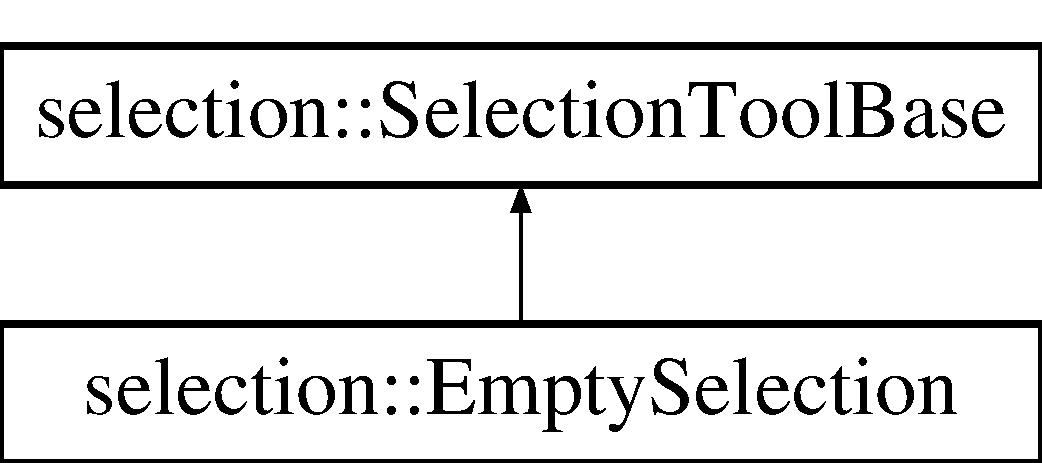
\includegraphics[height=2.000000cm]{classselection_1_1EmptySelection}
\end{center}
\end{figure}
\subsection*{Public Member Functions}
\begin{DoxyCompactItemize}
\item 
\hyperlink{classselection_1_1EmptySelection_a48affb4fc3524bf814304b3f439900fd}{Empty\-Selection} (const fhicl\-::\-Parameter\-Set \&pset)
\begin{DoxyCompactList}\small\item\em Constructor. \end{DoxyCompactList}\item 
\hypertarget{classselection_1_1EmptySelection_a62d52a58d6da0c8ae7723a405848bd5d}{\hyperlink{classselection_1_1EmptySelection_a62d52a58d6da0c8ae7723a405848bd5d}{$\sim$\-Empty\-Selection} ()}\label{classselection_1_1EmptySelection_a62d52a58d6da0c8ae7723a405848bd5d}

\begin{DoxyCompactList}\small\item\em Destructor. \end{DoxyCompactList}\item 
void \hyperlink{classselection_1_1EmptySelection_a065017fd69d7b8708752bfb1de50fcdc}{configure} (fhicl\-::\-Parameter\-Set const \&pset)
\item 
bool \hyperlink{classselection_1_1EmptySelection_a4ecce282e53d9d7c6c4764eef0b808f7}{select\-Event} (art\-::\-Event const \&e, const std\-::vector$<$ Proxy\-Pfp\-Elem\-\_\-t $>$ \&pfp\-\_\-pxy\-\_\-v)
\begin{DoxyCompactList}\small\item\em Selection function. \end{DoxyCompactList}\item 
\hypertarget{classselection_1_1EmptySelection_a5045b1b4c68a112effabf710714a2ea2}{void \hyperlink{classselection_1_1EmptySelection_a5045b1b4c68a112effabf710714a2ea2}{set\-Branches} (T\-Tree $\ast$\-\_\-tree)}\label{classselection_1_1EmptySelection_a5045b1b4c68a112effabf710714a2ea2}

\begin{DoxyCompactList}\small\item\em set branches for T\-Tree \end{DoxyCompactList}\item 
\hypertarget{classselection_1_1EmptySelection_aa1e91be25d006a7ff65765419a0667ea}{void \hyperlink{classselection_1_1EmptySelection_aa1e91be25d006a7ff65765419a0667ea}{reset\-T\-Tree} (T\-Tree $\ast$\-\_\-tree)}\label{classselection_1_1EmptySelection_aa1e91be25d006a7ff65765419a0667ea}

\begin{DoxyCompactList}\small\item\em reset ttree branches \end{DoxyCompactList}\end{DoxyCompactItemize}
\subsection*{Additional Inherited Members}


\subsection{Constructor \& Destructor Documentation}
\hypertarget{classselection_1_1EmptySelection_a48affb4fc3524bf814304b3f439900fd}{\index{selection\-::\-Empty\-Selection@{selection\-::\-Empty\-Selection}!Empty\-Selection@{Empty\-Selection}}
\index{Empty\-Selection@{Empty\-Selection}!selection::EmptySelection@{selection\-::\-Empty\-Selection}}
\subsubsection[{Empty\-Selection}]{\setlength{\rightskip}{0pt plus 5cm}selection\-::\-Empty\-Selection\-::\-Empty\-Selection (
\begin{DoxyParamCaption}
\item[{const fhicl\-::\-Parameter\-Set \&}]{pset}
\end{DoxyParamCaption}
)}}\label{classselection_1_1EmptySelection_a48affb4fc3524bf814304b3f439900fd}


Constructor. 


\begin{DoxyParams}{Parameters}
{\em pset} & Constructor.\\
\hline
\end{DoxyParams}
Arguments\-:

pset -\/ Fcl parameters. 

\subsection{Member Function Documentation}
\hypertarget{classselection_1_1EmptySelection_a065017fd69d7b8708752bfb1de50fcdc}{\index{selection\-::\-Empty\-Selection@{selection\-::\-Empty\-Selection}!configure@{configure}}
\index{configure@{configure}!selection::EmptySelection@{selection\-::\-Empty\-Selection}}
\subsubsection[{configure}]{\setlength{\rightskip}{0pt plus 5cm}void selection\-::\-Empty\-Selection\-::configure (
\begin{DoxyParamCaption}
\item[{fhicl\-::\-Parameter\-Set const \&}]{pset}
\end{DoxyParamCaption}
)}}\label{classselection_1_1EmptySelection_a065017fd69d7b8708752bfb1de50fcdc}
Reconfigure method.

Arguments\-:

pset -\/ Fcl parameter set. \hypertarget{classselection_1_1EmptySelection_a4ecce282e53d9d7c6c4764eef0b808f7}{\index{selection\-::\-Empty\-Selection@{selection\-::\-Empty\-Selection}!select\-Event@{select\-Event}}
\index{select\-Event@{select\-Event}!selection::EmptySelection@{selection\-::\-Empty\-Selection}}
\subsubsection[{select\-Event}]{\setlength{\rightskip}{0pt plus 5cm}bool selection\-::\-Empty\-Selection\-::select\-Event (
\begin{DoxyParamCaption}
\item[{art\-::\-Event const \&}]{e, }
\item[{const std\-::vector$<$ Proxy\-Pfp\-Elem\-\_\-t $>$ \&}]{pfp\-\_\-pxy\-\_\-v}
\end{DoxyParamCaption}
)\hspace{0.3cm}{\ttfamily [virtual]}}}\label{classselection_1_1EmptySelection_a4ecce282e53d9d7c6c4764eef0b808f7}


Selection function. 

Reconfigure method.

Arguments\-:

pset -\/ Fcl parameter set. 

Implements \hyperlink{classselection_1_1SelectionToolBase_ab63818dac49b43418fe9eb3b8cd98c9c}{selection\-::\-Selection\-Tool\-Base}.



The documentation for this class was generated from the following file\-:\begin{DoxyCompactItemize}
\item 
/home/travis/build/ubneutrinos/searchingfornues/\-Selection/\-Selection\-Tools/Empty\-Selection\-\_\-tool.\-cc\end{DoxyCompactItemize}

\hypertarget{classanalysis_1_1EventWeightTree}{}\section{analysis\+:\+:Event\+Weight\+Tree Class Reference}
\label{classanalysis_1_1EventWeightTree}\index{analysis\+::\+Event\+Weight\+Tree@{analysis\+::\+Event\+Weight\+Tree}}
Inheritance diagram for analysis\+:\+:Event\+Weight\+Tree\+:\begin{figure}[H]
\begin{center}
\leavevmode
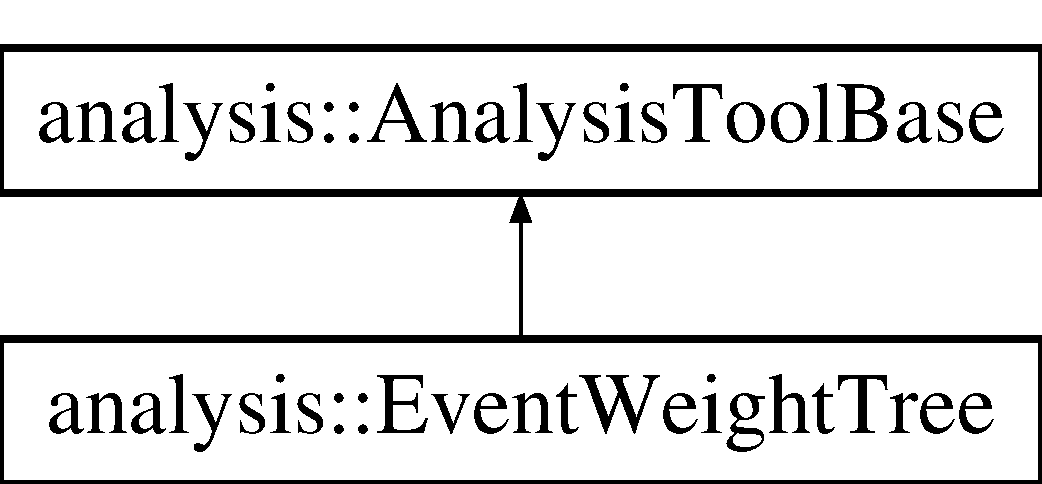
\includegraphics[height=2.000000cm]{classanalysis_1_1EventWeightTree}
\end{center}
\end{figure}
\subsection*{Public Member Functions}
\begin{DoxyCompactItemize}
\item 
\hyperlink{classanalysis_1_1EventWeightTree_a481af16f4e8721805bbe7fb5f0b1da2a}{Event\+Weight\+Tree} (const fhicl\+::\+Parameter\+Set \&pset)
\begin{DoxyCompactList}\small\item\em Constructor. \end{DoxyCompactList}\item 
\hyperlink{classanalysis_1_1EventWeightTree_ac4c13dc05b4378d910f25afdd410475b}{$\sim$\+Event\+Weight\+Tree} ()\hypertarget{classanalysis_1_1EventWeightTree_ac4c13dc05b4378d910f25afdd410475b}{}\label{classanalysis_1_1EventWeightTree_ac4c13dc05b4378d910f25afdd410475b}

\begin{DoxyCompactList}\small\item\em Destructor. \end{DoxyCompactList}\item 
void {\bfseries configure} (fhicl\+::\+Parameter\+Set const \&pset)\hypertarget{classanalysis_1_1EventWeightTree_a1998d34a8451a1e7ec8a6131fc50f97d}{}\label{classanalysis_1_1EventWeightTree_a1998d34a8451a1e7ec8a6131fc50f97d}

\item 
void \hyperlink{classanalysis_1_1EventWeightTree_a1af84126be9ecd2ae71013db4d2c1af7}{analyze\+Event} (art\+::\+Event const \&e, bool f\+Data) override\hypertarget{classanalysis_1_1EventWeightTree_a1af84126be9ecd2ae71013db4d2c1af7}{}\label{classanalysis_1_1EventWeightTree_a1af84126be9ecd2ae71013db4d2c1af7}

\begin{DoxyCompactList}\small\item\em Analysis function. \end{DoxyCompactList}\item 
void \hyperlink{classanalysis_1_1EventWeightTree_a2e30de7f19d6f20e6c3f7ffdb41b22a6}{analyze\+Slice} (art\+::\+Event const \&e, std\+::vector$<$ Proxy\+Pfp\+Elem\+\_\+t $>$ \&slice\+\_\+pfp\+\_\+v, bool f\+Data, bool selected) override\hypertarget{classanalysis_1_1EventWeightTree_a2e30de7f19d6f20e6c3f7ffdb41b22a6}{}\label{classanalysis_1_1EventWeightTree_a2e30de7f19d6f20e6c3f7ffdb41b22a6}

\begin{DoxyCompactList}\small\item\em Analyze slice. \end{DoxyCompactList}\item 
void \hyperlink{classanalysis_1_1EventWeightTree_a7f86ad4b26cab90a5e90a84d57530a26}{set\+Branches} (T\+Tree $\ast$\+\_\+tree) override\hypertarget{classanalysis_1_1EventWeightTree_a7f86ad4b26cab90a5e90a84d57530a26}{}\label{classanalysis_1_1EventWeightTree_a7f86ad4b26cab90a5e90a84d57530a26}

\begin{DoxyCompactList}\small\item\em set branches for T\+Tree \end{DoxyCompactList}\item 
void \hyperlink{classanalysis_1_1EventWeightTree_a1f2a0ae51f500a3e4d0690f9b16505da}{reset\+T\+Tree} (T\+Tree $\ast$\+\_\+tree) override\hypertarget{classanalysis_1_1EventWeightTree_a1f2a0ae51f500a3e4d0690f9b16505da}{}\label{classanalysis_1_1EventWeightTree_a1f2a0ae51f500a3e4d0690f9b16505da}

\begin{DoxyCompactList}\small\item\em reset ttree branches \end{DoxyCompactList}\end{DoxyCompactItemize}
\subsection*{Private Attributes}
\begin{DoxyCompactItemize}
\item 
T\+Tree $\ast$ {\bfseries \+\_\+weightstree}\hypertarget{classanalysis_1_1EventWeightTree_a007ac1f04819cff64bb54b6206966408}{}\label{classanalysis_1_1EventWeightTree_a007ac1f04819cff64bb54b6206966408}

\item 
std\+::map$<$ std\+::string, std\+::vector$<$ double $>$ $>$ {\bfseries \+\_\+map\+Weight}\hypertarget{classanalysis_1_1EventWeightTree_aef493db93e72288ef19cd155052fbce6}{}\label{classanalysis_1_1EventWeightTree_aef493db93e72288ef19cd155052fbce6}

\item 
std\+::vector$<$ double $>$ {\bfseries \+\_\+vec\+Weight\+Flux}\hypertarget{classanalysis_1_1EventWeightTree_a63fcb54ac96617bfa03f1c98bc941d47}{}\label{classanalysis_1_1EventWeightTree_a63fcb54ac96617bfa03f1c98bc941d47}

\item 
std\+::vector$<$ double $>$ {\bfseries \+\_\+vec\+Weights\+Genie}\hypertarget{classanalysis_1_1EventWeightTree_a27f4bcfa903da58796010d056b257f1c}{}\label{classanalysis_1_1EventWeightTree_a27f4bcfa903da58796010d056b257f1c}

\item 
std\+::vector$<$ double $>$ {\bfseries \+\_\+vec\+Weights\+Reint}\hypertarget{classanalysis_1_1EventWeightTree_a2afa517c5d3c82f395cca60f6bed1e55}{}\label{classanalysis_1_1EventWeightTree_a2afa517c5d3c82f395cca60f6bed1e55}

\item 
float {\bfseries \+\_\+weight\+Spline}\hypertarget{classanalysis_1_1EventWeightTree_a5f616b70e5653cd00a2beda1da0db13f}{}\label{classanalysis_1_1EventWeightTree_a5f616b70e5653cd00a2beda1da0db13f}

\item 
bool {\bfseries \+\_\+create\+Dedicated\+Tree}\hypertarget{classanalysis_1_1EventWeightTree_a2ae36b271ba94dcdfcaafd0d3d9f4550}{}\label{classanalysis_1_1EventWeightTree_a2ae36b271ba94dcdfcaafd0d3d9f4550}

\item 
bool {\bfseries \+\_\+create\+Map\+Branch}\hypertarget{classanalysis_1_1EventWeightTree_ac0eeccf0e01dde3c1d0e97674dcbfbb9}{}\label{classanalysis_1_1EventWeightTree_ac0eeccf0e01dde3c1d0e97674dcbfbb9}

\item 
bool {\bfseries \+\_\+create\+Flux\+Branch}\hypertarget{classanalysis_1_1EventWeightTree_a2905d3ca10c17a92cef96d00c9b65801}{}\label{classanalysis_1_1EventWeightTree_a2905d3ca10c17a92cef96d00c9b65801}

\item 
bool {\bfseries \+\_\+create\+Genie\+Branch}\hypertarget{classanalysis_1_1EventWeightTree_af66736f8bc62c7b29fcca28576132c0e}{}\label{classanalysis_1_1EventWeightTree_af66736f8bc62c7b29fcca28576132c0e}

\item 
bool {\bfseries \+\_\+create\+Reint\+Branch}\hypertarget{classanalysis_1_1EventWeightTree_a30a5f48b802fcf22092caf532a1bb6f9}{}\label{classanalysis_1_1EventWeightTree_a30a5f48b802fcf22092caf532a1bb6f9}

\item 
bool {\bfseries \+\_\+create\+Spline\+Branch}\hypertarget{classanalysis_1_1EventWeightTree_a20a763fab2d058c9742b9101e90da819}{}\label{classanalysis_1_1EventWeightTree_a20a763fab2d058c9742b9101e90da819}

\item 
int {\bfseries \+\_\+run}\hypertarget{classanalysis_1_1EventWeightTree_ac52e040d9ffac87eeeb4222fe175338b}{}\label{classanalysis_1_1EventWeightTree_ac52e040d9ffac87eeeb4222fe175338b}

\item 
int {\bfseries \+\_\+sub\+Run}\hypertarget{classanalysis_1_1EventWeightTree_a6d993a5f48707b15251e6c615f83be14}{}\label{classanalysis_1_1EventWeightTree_a6d993a5f48707b15251e6c615f83be14}

\item 
int {\bfseries \+\_\+evt}\hypertarget{classanalysis_1_1EventWeightTree_aea12ca02fb94fe73ae1da0ef9f8682aa}{}\label{classanalysis_1_1EventWeightTree_aea12ca02fb94fe73ae1da0ef9f8682aa}

\end{DoxyCompactItemize}


\subsection{Constructor \& Destructor Documentation}
\index{analysis\+::\+Event\+Weight\+Tree@{analysis\+::\+Event\+Weight\+Tree}!Event\+Weight\+Tree@{Event\+Weight\+Tree}}
\index{Event\+Weight\+Tree@{Event\+Weight\+Tree}!analysis\+::\+Event\+Weight\+Tree@{analysis\+::\+Event\+Weight\+Tree}}
\subsubsection[{\texorpdfstring{Event\+Weight\+Tree(const fhicl\+::\+Parameter\+Set \&pset)}{EventWeightTree(const fhicl::ParameterSet &pset)}}]{\setlength{\rightskip}{0pt plus 5cm}analysis\+::\+Event\+Weight\+Tree\+::\+Event\+Weight\+Tree (
\begin{DoxyParamCaption}
\item[{const fhicl\+::\+Parameter\+Set \&}]{pset}
\end{DoxyParamCaption}
)}\hypertarget{classanalysis_1_1EventWeightTree_a481af16f4e8721805bbe7fb5f0b1da2a}{}\label{classanalysis_1_1EventWeightTree_a481af16f4e8721805bbe7fb5f0b1da2a}


Constructor. 


\begin{DoxyParams}{Parameters}
{\em pset} & \\
\hline
\end{DoxyParams}


The documentation for this class was generated from the following file\+:\begin{DoxyCompactItemize}
\item 
/home/travis/build/ubneutrinos/searchingfornues/\+Selection/\+Analysis\+Tools/Event\+Weight\+Tree\+\_\+tool.\+cc\end{DoxyCompactItemize}

\hypertarget{classflashmatch_1_1FlashMatchingTool_1_1FailureMode}{}\section{flashmatch\+:\+:Flash\+Matching\+Tool\+:\+:Failure\+Mode Class Reference}
\label{classflashmatch_1_1FlashMatchingTool_1_1FailureMode}\index{flashmatch\+::\+Flash\+Matching\+Tool\+::\+Failure\+Mode@{flashmatch\+::\+Flash\+Matching\+Tool\+::\+Failure\+Mode}}


A description of the reason the tool couldn\textquotesingle{}t find a neutrino candidate.  


\subsection*{Public Member Functions}
\begin{DoxyCompactItemize}
\item 
\hyperlink{classflashmatch_1_1FlashMatchingTool_1_1FailureMode_adcdc5adb8c7321605b8f9ef7740ea209}{Failure\+Mode} (const std\+::string \&reason)
\begin{DoxyCompactList}\small\item\em Default constructor. \end{DoxyCompactList}\item 
\hyperlink{classflashmatch_1_1FlashMatchingTool_1_1FailureMode_ab6ee2b8304974614e71440359a068acd}{$\sim$\+Failure\+Mode} ()\hypertarget{classflashmatch_1_1FlashMatchingTool_1_1FailureMode_ab6ee2b8304974614e71440359a068acd}{}\label{classflashmatch_1_1FlashMatchingTool_1_1FailureMode_ab6ee2b8304974614e71440359a068acd}

\begin{DoxyCompactList}\small\item\em Default destructor -\/ explains the failure. \end{DoxyCompactList}\item 
void {\bfseries Print} ()\hypertarget{classflashmatch_1_1FlashMatchingTool_1_1FailureMode_a2e0b3138a293e90410b3037952c819bc}{}\label{classflashmatch_1_1FlashMatchingTool_1_1FailureMode_a2e0b3138a293e90410b3037952c819bc}

\end{DoxyCompactItemize}
\subsection*{Private Attributes}
\begin{DoxyCompactItemize}
\item 
std\+::string \hyperlink{classflashmatch_1_1FlashMatchingTool_1_1FailureMode_ad236e712ac187b60a5647ad4bf29cf07}{m\+\_\+reason}\hypertarget{classflashmatch_1_1FlashMatchingTool_1_1FailureMode_ad236e712ac187b60a5647ad4bf29cf07}{}\label{classflashmatch_1_1FlashMatchingTool_1_1FailureMode_ad236e712ac187b60a5647ad4bf29cf07}

\begin{DoxyCompactList}\small\item\em The reason for the failure. \end{DoxyCompactList}\end{DoxyCompactItemize}


\subsection{Detailed Description}
A description of the reason the tool couldn\textquotesingle{}t find a neutrino candidate. 

\subsection{Constructor \& Destructor Documentation}
\index{flashmatch\+::\+Flash\+Matching\+Tool\+::\+Failure\+Mode@{flashmatch\+::\+Flash\+Matching\+Tool\+::\+Failure\+Mode}!Failure\+Mode@{Failure\+Mode}}
\index{Failure\+Mode@{Failure\+Mode}!flashmatch\+::\+Flash\+Matching\+Tool\+::\+Failure\+Mode@{flashmatch\+::\+Flash\+Matching\+Tool\+::\+Failure\+Mode}}
\subsubsection[{\texorpdfstring{Failure\+Mode(const std\+::string \&reason)}{FailureMode(const std::string &reason)}}]{\setlength{\rightskip}{0pt plus 5cm}flashmatch\+::\+Flash\+Matching\+Tool\+::\+Failure\+Mode\+::\+Failure\+Mode (
\begin{DoxyParamCaption}
\item[{const std\+::string \&}]{reason}
\end{DoxyParamCaption}
)\hspace{0.3cm}{\ttfamily [inline]}}\hypertarget{classflashmatch_1_1FlashMatchingTool_1_1FailureMode_adcdc5adb8c7321605b8f9ef7740ea209}{}\label{classflashmatch_1_1FlashMatchingTool_1_1FailureMode_adcdc5adb8c7321605b8f9ef7740ea209}


Default constructor. 


\begin{DoxyParams}{Parameters}
{\em reason} & the reason for the failure \\
\hline
\end{DoxyParams}


The documentation for this class was generated from the following file\+:\begin{DoxyCompactItemize}
\item 
/home/travis/build/ubneutrinos/searchingfornues/\+Flash\+Matching/Flash\+Matching\+Tool\+\_\+tool.\+cc\end{DoxyCompactItemize}

\hypertarget{classflashmatch_1_1FlashMatchingTool_1_1FlashCandidate}{\section{flashmatch\-:\-:Flash\-Matching\-Tool\-:\-:Flash\-Candidate Class Reference}
\label{classflashmatch_1_1FlashMatchingTool_1_1FlashCandidate}\index{flashmatch\-::\-Flash\-Matching\-Tool\-::\-Flash\-Candidate@{flashmatch\-::\-Flash\-Matching\-Tool\-::\-Flash\-Candidate}}
}


A candidate for the beam flash.  


\subsection*{Public Member Functions}
\begin{DoxyCompactItemize}
\item 
\hypertarget{classflashmatch_1_1FlashMatchingTool_1_1FlashCandidate_a2d514815c7f1cd16cec72f45781b9532}{\hyperlink{classflashmatch_1_1FlashMatchingTool_1_1FlashCandidate_a2d514815c7f1cd16cec72f45781b9532}{Flash\-Candidate} ()}\label{classflashmatch_1_1FlashMatchingTool_1_1FlashCandidate_a2d514815c7f1cd16cec72f45781b9532}

\begin{DoxyCompactList}\small\item\em Default constructor. \end{DoxyCompactList}\item 
\hyperlink{classflashmatch_1_1FlashMatchingTool_1_1FlashCandidate_a95fa2be25e8635d56d6768b2886fa821}{Flash\-Candidate} (const art\-::\-Event \&event, const recob\-::\-Op\-Flash \&flash)
\begin{DoxyCompactList}\small\item\em Parametrized constructor. \end{DoxyCompactList}\item 
bool \hyperlink{classflashmatch_1_1FlashMatchingTool_1_1FlashCandidate_abe37a111abddadacef277af4f8adda44}{Is\-In\-Beam\-Window} (const float beam\-Window\-Start, const float beam\-Window\-End)
\begin{DoxyCompactList}\small\item\em Check if the time of the flash is in the beam window, and save the information for later. \end{DoxyCompactList}\item 
bool \hyperlink{classflashmatch_1_1FlashMatchingTool_1_1FlashCandidate_a43b731e560f75645df5aa5d74f017ba0}{Passes\-P\-E\-Threshold} (const float min\-Beam\-Flash\-P\-E) const 
\begin{DoxyCompactList}\small\item\em Check if the flash passes the minimum P\-E threshold. \end{DoxyCompactList}\item 
flashana\-::\-Flash\-\_\-t \hyperlink{classflashmatch_1_1FlashMatchingTool_1_1FlashCandidate_ab8156ee16d27febb44352c4ffd6adf56}{Convert\-Flash\-Format} () const 
\end{DoxyCompactItemize}
\subsection*{Public Attributes}
\begin{DoxyCompactItemize}
\item 
\hypertarget{classflashmatch_1_1FlashMatchingTool_1_1FlashCandidate_ae9d4df4f83da1b8115f7efe9af9438f8}{int \hyperlink{classflashmatch_1_1FlashMatchingTool_1_1FlashCandidate_ae9d4df4f83da1b8115f7efe9af9438f8}{m\-\_\-run}}\label{classflashmatch_1_1FlashMatchingTool_1_1FlashCandidate_ae9d4df4f83da1b8115f7efe9af9438f8}

\begin{DoxyCompactList}\small\item\em The run number. \end{DoxyCompactList}\item 
\hypertarget{classflashmatch_1_1FlashMatchingTool_1_1FlashCandidate_a033d91e33897a3ca874b47df76c15b5b}{int \hyperlink{classflashmatch_1_1FlashMatchingTool_1_1FlashCandidate_a033d91e33897a3ca874b47df76c15b5b}{m\-\_\-sub\-Run}}\label{classflashmatch_1_1FlashMatchingTool_1_1FlashCandidate_a033d91e33897a3ca874b47df76c15b5b}

\begin{DoxyCompactList}\small\item\em The sub\-Run number. \end{DoxyCompactList}\item 
\hypertarget{classflashmatch_1_1FlashMatchingTool_1_1FlashCandidate_a37e853b88c41a9f253226a42e10cb6f7}{int \hyperlink{classflashmatch_1_1FlashMatchingTool_1_1FlashCandidate_a37e853b88c41a9f253226a42e10cb6f7}{m\-\_\-event}}\label{classflashmatch_1_1FlashMatchingTool_1_1FlashCandidate_a37e853b88c41a9f253226a42e10cb6f7}

\begin{DoxyCompactList}\small\item\em The event number. \end{DoxyCompactList}\item 
\hypertarget{classflashmatch_1_1FlashMatchingTool_1_1FlashCandidate_a8fd909c9684798b9e6e6b71a3f1af7f4}{float \hyperlink{classflashmatch_1_1FlashMatchingTool_1_1FlashCandidate_a8fd909c9684798b9e6e6b71a3f1af7f4}{m\-\_\-time}}\label{classflashmatch_1_1FlashMatchingTool_1_1FlashCandidate_a8fd909c9684798b9e6e6b71a3f1af7f4}

\begin{DoxyCompactList}\small\item\em Time of the flash. \end{DoxyCompactList}\item 
\hypertarget{classflashmatch_1_1FlashMatchingTool_1_1FlashCandidate_ace7b40b6d8ae1ebe7ea88314ea855a74}{std\-::vector$<$ float $>$ \hyperlink{classflashmatch_1_1FlashMatchingTool_1_1FlashCandidate_ace7b40b6d8ae1ebe7ea88314ea855a74}{m\-\_\-pe\-Spectrum}}\label{classflashmatch_1_1FlashMatchingTool_1_1FlashCandidate_ace7b40b6d8ae1ebe7ea88314ea855a74}

\begin{DoxyCompactList}\small\item\em The number of P\-Es on each P\-M\-T. \end{DoxyCompactList}\item 
\hypertarget{classflashmatch_1_1FlashMatchingTool_1_1FlashCandidate_a3ecf14f425f49452494ece572ef97927}{std\-::vector$<$ float $>$ \hyperlink{classflashmatch_1_1FlashMatchingTool_1_1FlashCandidate_a3ecf14f425f49452494ece572ef97927}{m\-\_\-pe\-Hyp\-Spectrum}}\label{classflashmatch_1_1FlashMatchingTool_1_1FlashCandidate_a3ecf14f425f49452494ece572ef97927}

\begin{DoxyCompactList}\small\item\em The number of P\-Es on each P\-M\-T. \end{DoxyCompactList}\item 
\hypertarget{classflashmatch_1_1FlashMatchingTool_1_1FlashCandidate_a5193b7f6862ca08d3dd91a16f2ade309}{float \hyperlink{classflashmatch_1_1FlashMatchingTool_1_1FlashCandidate_a5193b7f6862ca08d3dd91a16f2ade309}{m\-\_\-total\-P\-E}}\label{classflashmatch_1_1FlashMatchingTool_1_1FlashCandidate_a5193b7f6862ca08d3dd91a16f2ade309}

\begin{DoxyCompactList}\small\item\em The total number of photoelectrons over all P\-M\-Ts in the flash. \end{DoxyCompactList}\item 
\hypertarget{classflashmatch_1_1FlashMatchingTool_1_1FlashCandidate_ac75a41fb6afaab35cee4510d76bf6405}{float \hyperlink{classflashmatch_1_1FlashMatchingTool_1_1FlashCandidate_ac75a41fb6afaab35cee4510d76bf6405}{m\-\_\-center\-Y}}\label{classflashmatch_1_1FlashMatchingTool_1_1FlashCandidate_ac75a41fb6afaab35cee4510d76bf6405}

\begin{DoxyCompactList}\small\item\em The P\-E weighted center Y position of the flash. \end{DoxyCompactList}\item 
\hypertarget{classflashmatch_1_1FlashMatchingTool_1_1FlashCandidate_afdc868f23ccd16c5528548163d7ec2a7}{float \hyperlink{classflashmatch_1_1FlashMatchingTool_1_1FlashCandidate_afdc868f23ccd16c5528548163d7ec2a7}{m\-\_\-center\-Z}}\label{classflashmatch_1_1FlashMatchingTool_1_1FlashCandidate_afdc868f23ccd16c5528548163d7ec2a7}

\begin{DoxyCompactList}\small\item\em The P\-E weighted center Z position of the flash. \end{DoxyCompactList}\item 
\hypertarget{classflashmatch_1_1FlashMatchingTool_1_1FlashCandidate_a80fccdaaa6a851437fe16e9c4e855ea3}{float \hyperlink{classflashmatch_1_1FlashMatchingTool_1_1FlashCandidate_a80fccdaaa6a851437fe16e9c4e855ea3}{m\-\_\-width\-Y}}\label{classflashmatch_1_1FlashMatchingTool_1_1FlashCandidate_a80fccdaaa6a851437fe16e9c4e855ea3}

\begin{DoxyCompactList}\small\item\em The P\-E weighted width of the flash in Y. \end{DoxyCompactList}\item 
\hypertarget{classflashmatch_1_1FlashMatchingTool_1_1FlashCandidate_a766f8587c3ab476751755089f4089b64}{float \hyperlink{classflashmatch_1_1FlashMatchingTool_1_1FlashCandidate_a766f8587c3ab476751755089f4089b64}{m\-\_\-width\-Z}}\label{classflashmatch_1_1FlashMatchingTool_1_1FlashCandidate_a766f8587c3ab476751755089f4089b64}

\begin{DoxyCompactList}\small\item\em The P\-E weighted width of the flash in Z. \end{DoxyCompactList}\item 
\hypertarget{classflashmatch_1_1FlashMatchingTool_1_1FlashCandidate_aa5d463fd9635e66a8e968ca979b0c451}{bool \hyperlink{classflashmatch_1_1FlashMatchingTool_1_1FlashCandidate_aa5d463fd9635e66a8e968ca979b0c451}{m\-\_\-in\-Beam\-Window}}\label{classflashmatch_1_1FlashMatchingTool_1_1FlashCandidate_aa5d463fd9635e66a8e968ca979b0c451}

\begin{DoxyCompactList}\small\item\em If the flash is in time with the beam window. \end{DoxyCompactList}\item 
\hypertarget{classflashmatch_1_1FlashMatchingTool_1_1FlashCandidate_aa169ff8ec85fb81e3c74e82e2ef1cb52}{bool \hyperlink{classflashmatch_1_1FlashMatchingTool_1_1FlashCandidate_aa169ff8ec85fb81e3c74e82e2ef1cb52}{m\-\_\-is\-Brightest\-In\-Window}}\label{classflashmatch_1_1FlashMatchingTool_1_1FlashCandidate_aa169ff8ec85fb81e3c74e82e2ef1cb52}

\begin{DoxyCompactList}\small\item\em If the flash is the brightest in the event. \end{DoxyCompactList}\item 
\hypertarget{classflashmatch_1_1FlashMatchingTool_1_1FlashCandidate_a893039a92d032f20f57156f5c2c2299a}{bool \hyperlink{classflashmatch_1_1FlashMatchingTool_1_1FlashCandidate_a893039a92d032f20f57156f5c2c2299a}{m\-\_\-is\-Beam\-Flash}}\label{classflashmatch_1_1FlashMatchingTool_1_1FlashCandidate_a893039a92d032f20f57156f5c2c2299a}

\begin{DoxyCompactList}\small\item\em If the flash has been selected as the beam flash. \end{DoxyCompactList}\end{DoxyCompactItemize}


\subsection{Detailed Description}
A candidate for the beam flash. 

\subsection{Constructor \& Destructor Documentation}
\hypertarget{classflashmatch_1_1FlashMatchingTool_1_1FlashCandidate_a95fa2be25e8635d56d6768b2886fa821}{\index{flashmatch\-::\-Flash\-Matching\-Tool\-::\-Flash\-Candidate@{flashmatch\-::\-Flash\-Matching\-Tool\-::\-Flash\-Candidate}!Flash\-Candidate@{Flash\-Candidate}}
\index{Flash\-Candidate@{Flash\-Candidate}!flashmatch::FlashMatchingTool::FlashCandidate@{flashmatch\-::\-Flash\-Matching\-Tool\-::\-Flash\-Candidate}}
\subsubsection[{Flash\-Candidate}]{\setlength{\rightskip}{0pt plus 5cm}flashmatch\-::\-Flash\-Matching\-Tool\-::\-Flash\-Candidate\-::\-Flash\-Candidate (
\begin{DoxyParamCaption}
\item[{const art\-::\-Event \&}]{event, }
\item[{const recob\-::\-Op\-Flash \&}]{flash}
\end{DoxyParamCaption}
)\hspace{0.3cm}{\ttfamily [inline]}}}\label{classflashmatch_1_1FlashMatchingTool_1_1FlashCandidate_a95fa2be25e8635d56d6768b2886fa821}


Parametrized constructor. 


\begin{DoxyParams}{Parameters}
{\em event} & the art event \\
\hline
{\em flash} & the flash \\
\hline
\end{DoxyParams}


\subsection{Member Function Documentation}
\hypertarget{classflashmatch_1_1FlashMatchingTool_1_1FlashCandidate_ab8156ee16d27febb44352c4ffd6adf56}{\index{flashmatch\-::\-Flash\-Matching\-Tool\-::\-Flash\-Candidate@{flashmatch\-::\-Flash\-Matching\-Tool\-::\-Flash\-Candidate}!Convert\-Flash\-Format@{Convert\-Flash\-Format}}
\index{Convert\-Flash\-Format@{Convert\-Flash\-Format}!flashmatch::FlashMatchingTool::FlashCandidate@{flashmatch\-::\-Flash\-Matching\-Tool\-::\-Flash\-Candidate}}
\subsubsection[{Convert\-Flash\-Format}]{\setlength{\rightskip}{0pt plus 5cm}flashana\-::\-Flash\-\_\-t flashmatch\-::\-Flash\-Matching\-Tool\-::\-Flash\-Candidate\-::\-Convert\-Flash\-Format (
\begin{DoxyParamCaption}
{}
\end{DoxyParamCaption}
) const\hspace{0.3cm}{\ttfamily [inline]}}}\label{classflashmatch_1_1FlashMatchingTool_1_1FlashCandidate_ab8156ee16d27febb44352c4ffd6adf56}
Convert to a flashana\-::\-Flash\-\_\-t

\begin{DoxyReturn}{Returns}
the flashana\-::\-Flash\-\_\-t 
\end{DoxyReturn}
\hypertarget{classflashmatch_1_1FlashMatchingTool_1_1FlashCandidate_abe37a111abddadacef277af4f8adda44}{\index{flashmatch\-::\-Flash\-Matching\-Tool\-::\-Flash\-Candidate@{flashmatch\-::\-Flash\-Matching\-Tool\-::\-Flash\-Candidate}!Is\-In\-Beam\-Window@{Is\-In\-Beam\-Window}}
\index{Is\-In\-Beam\-Window@{Is\-In\-Beam\-Window}!flashmatch::FlashMatchingTool::FlashCandidate@{flashmatch\-::\-Flash\-Matching\-Tool\-::\-Flash\-Candidate}}
\subsubsection[{Is\-In\-Beam\-Window}]{\setlength{\rightskip}{0pt plus 5cm}bool flashmatch\-::\-Flash\-Matching\-Tool\-::\-Flash\-Candidate\-::\-Is\-In\-Beam\-Window (
\begin{DoxyParamCaption}
\item[{const float}]{beam\-Window\-Start, }
\item[{const float}]{beam\-Window\-End}
\end{DoxyParamCaption}
)\hspace{0.3cm}{\ttfamily [inline]}}}\label{classflashmatch_1_1FlashMatchingTool_1_1FlashCandidate_abe37a111abddadacef277af4f8adda44}


Check if the time of the flash is in the beam window, and save the information for later. 


\begin{DoxyParams}{Parameters}
{\em beam\-Window\-Start} & the starting time of the beam window \\
\hline
{\em beam\-Window\-Wend} & the end time of the beam window \\
\hline
\end{DoxyParams}
\hypertarget{classflashmatch_1_1FlashMatchingTool_1_1FlashCandidate_a43b731e560f75645df5aa5d74f017ba0}{\index{flashmatch\-::\-Flash\-Matching\-Tool\-::\-Flash\-Candidate@{flashmatch\-::\-Flash\-Matching\-Tool\-::\-Flash\-Candidate}!Passes\-P\-E\-Threshold@{Passes\-P\-E\-Threshold}}
\index{Passes\-P\-E\-Threshold@{Passes\-P\-E\-Threshold}!flashmatch::FlashMatchingTool::FlashCandidate@{flashmatch\-::\-Flash\-Matching\-Tool\-::\-Flash\-Candidate}}
\subsubsection[{Passes\-P\-E\-Threshold}]{\setlength{\rightskip}{0pt plus 5cm}bool flashmatch\-::\-Flash\-Matching\-Tool\-::\-Flash\-Candidate\-::\-Passes\-P\-E\-Threshold (
\begin{DoxyParamCaption}
\item[{const float}]{min\-Beam\-Flash\-P\-E}
\end{DoxyParamCaption}
) const\hspace{0.3cm}{\ttfamily [inline]}}}\label{classflashmatch_1_1FlashMatchingTool_1_1FlashCandidate_a43b731e560f75645df5aa5d74f017ba0}


Check if the flash passes the minimum P\-E threshold. 


\begin{DoxyParams}{Parameters}
{\em min\-Beam\-Flash\-P\-E} & the minimum number of photo electrons to pass \\
\hline
\end{DoxyParams}


The documentation for this class was generated from the following file\-:\begin{DoxyCompactItemize}
\item 
/home/travis/build/ubneutrinos/searchingfornues/\-Flash\-Matching/Flash\-Matching\-Tool\-\_\-tool.\-cc\end{DoxyCompactItemize}

\hypertarget{classanalysis_1_1FlashMatching}{\section{analysis\-:\-:Flash\-Matching Class Reference}
\label{classanalysis_1_1FlashMatching}\index{analysis\-::\-Flash\-Matching@{analysis\-::\-Flash\-Matching}}
}
Inheritance diagram for analysis\-:\-:Flash\-Matching\-:\begin{figure}[H]
\begin{center}
\leavevmode
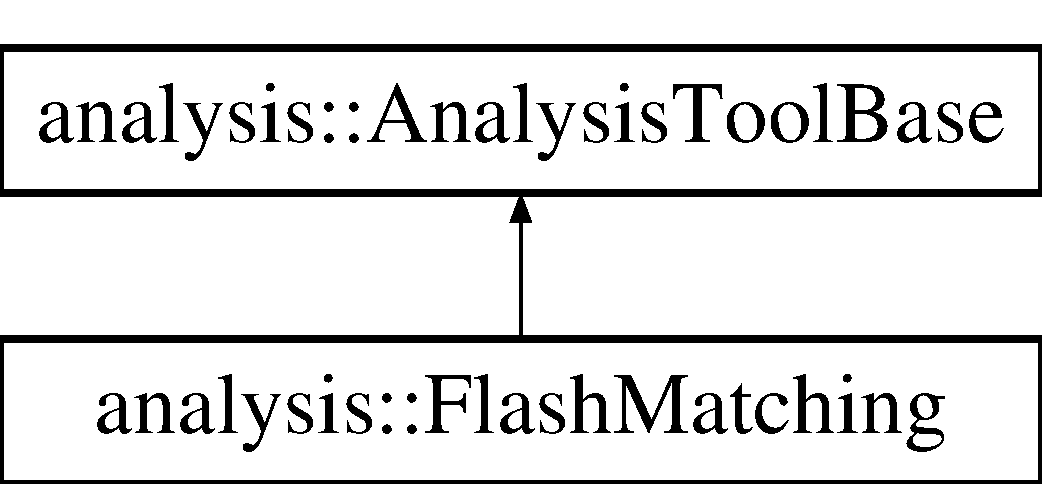
\includegraphics[height=2.000000cm]{classanalysis_1_1FlashMatching}
\end{center}
\end{figure}
\subsection*{Public Member Functions}
\begin{DoxyCompactItemize}
\item 
\hyperlink{classanalysis_1_1FlashMatching_a00eb9eca115b63fe442d1a14fb205692}{Flash\-Matching} (const fhicl\-::\-Parameter\-Set \&pset)
\begin{DoxyCompactList}\small\item\em Constructor. \end{DoxyCompactList}\item 
\hypertarget{classanalysis_1_1FlashMatching_ab2647643c3420bac36afe949ac252f20}{\hyperlink{classanalysis_1_1FlashMatching_ab2647643c3420bac36afe949ac252f20}{$\sim$\-Flash\-Matching} ()}\label{classanalysis_1_1FlashMatching_ab2647643c3420bac36afe949ac252f20}

\begin{DoxyCompactList}\small\item\em Destructor. \end{DoxyCompactList}\item 
void \hyperlink{classanalysis_1_1FlashMatching_a313d8dd41d24540555aaf27e87579626}{configure} (fhicl\-::\-Parameter\-Set const \&pset)
\item 
\hypertarget{classanalysis_1_1FlashMatching_ab3bc034486cadaeda1c4c0868a7f17f1}{void \hyperlink{classanalysis_1_1FlashMatching_ab3bc034486cadaeda1c4c0868a7f17f1}{analyze\-Event} (art\-::\-Event const \&e, bool f\-Data) override}\label{classanalysis_1_1FlashMatching_ab3bc034486cadaeda1c4c0868a7f17f1}

\begin{DoxyCompactList}\small\item\em Analysis function. \end{DoxyCompactList}\item 
void \hyperlink{classanalysis_1_1FlashMatching_acdff3053951979de66145a37a41f1767}{analyze\-Slice} (art\-::\-Event const \&e, std\-::vector$<$ Proxy\-Pfp\-Elem\-\_\-t $>$ \&slice\-\_\-pfp\-\_\-v, bool f\-Data, bool selected) override
\begin{DoxyCompactList}\small\item\em Analyze slice. \end{DoxyCompactList}\item 
\hypertarget{classanalysis_1_1FlashMatching_a40570b8e39ad953ba6acccbe5c466c49}{void \hyperlink{classanalysis_1_1FlashMatching_a40570b8e39ad953ba6acccbe5c466c49}{set\-Branches} (T\-Tree $\ast$\-\_\-tree) override}\label{classanalysis_1_1FlashMatching_a40570b8e39ad953ba6acccbe5c466c49}

\begin{DoxyCompactList}\small\item\em set branches for T\-Tree \end{DoxyCompactList}\item 
\hypertarget{classanalysis_1_1FlashMatching_ac9f3186d0a7acb4723959687710f7bab}{void \hyperlink{classanalysis_1_1FlashMatching_ac9f3186d0a7acb4723959687710f7bab}{reset\-T\-Tree} (T\-Tree $\ast$\-\_\-tree) override}\label{classanalysis_1_1FlashMatching_ac9f3186d0a7acb4723959687710f7bab}

\begin{DoxyCompactList}\small\item\em reset ttree branches \end{DoxyCompactList}\end{DoxyCompactItemize}
\subsection*{Private Attributes}
\begin{DoxyCompactItemize}
\item 
\hypertarget{classanalysis_1_1FlashMatching_ab08a41fbfa79153063d300f2f00cf2ce}{art\-::\-Input\-Tag {\bfseries f\-P\-F\-Pproducer}}\label{classanalysis_1_1FlashMatching_ab08a41fbfa79153063d300f2f00cf2ce}

\item 
\hypertarget{classanalysis_1_1FlashMatching_adc40aeaba0f5c6e5db982a2630a5c869}{art\-::\-Input\-Tag {\bfseries f\-T0producer}}\label{classanalysis_1_1FlashMatching_adc40aeaba0f5c6e5db982a2630a5c869}

\item 
\hypertarget{classanalysis_1_1FlashMatching_ad5378659d44adbf60961370b7e09059f}{float {\bfseries \-\_\-nu\-\_\-flashmatch\-\_\-score}}\label{classanalysis_1_1FlashMatching_ad5378659d44adbf60961370b7e09059f}

\item 
\hypertarget{classanalysis_1_1FlashMatching_a1272dc1455e89eea53d439c1789562c5}{float {\bfseries \-\_\-best\-\_\-cosmic\-\_\-flashmatch\-\_\-score}}\label{classanalysis_1_1FlashMatching_a1272dc1455e89eea53d439c1789562c5}

\item 
\hypertarget{classanalysis_1_1FlashMatching_a37d29c4362498710cb68584518ee4ec6}{float {\bfseries \-\_\-best\-\_\-obviouscosmic\-\_\-flashmatch\-\_\-score}}\label{classanalysis_1_1FlashMatching_a37d29c4362498710cb68584518ee4ec6}

\item 
\hypertarget{classanalysis_1_1FlashMatching_a4a23f572bbc5503c07fdd410d7742598}{std\-::vector$<$ float $>$ {\bfseries \-\_\-cosmic\-\_\-flashmatch\-\_\-score\-\_\-v}}\label{classanalysis_1_1FlashMatching_a4a23f572bbc5503c07fdd410d7742598}

\end{DoxyCompactItemize}


\subsection{Constructor \& Destructor Documentation}
\hypertarget{classanalysis_1_1FlashMatching_a00eb9eca115b63fe442d1a14fb205692}{\index{analysis\-::\-Flash\-Matching@{analysis\-::\-Flash\-Matching}!Flash\-Matching@{Flash\-Matching}}
\index{Flash\-Matching@{Flash\-Matching}!analysis::FlashMatching@{analysis\-::\-Flash\-Matching}}
\subsubsection[{Flash\-Matching}]{\setlength{\rightskip}{0pt plus 5cm}analysis\-::\-Flash\-Matching\-::\-Flash\-Matching (
\begin{DoxyParamCaption}
\item[{const fhicl\-::\-Parameter\-Set \&}]{p}
\end{DoxyParamCaption}
)}}\label{classanalysis_1_1FlashMatching_a00eb9eca115b63fe442d1a14fb205692}


Constructor. 


\begin{DoxyParams}{Parameters}
{\em pset} & Constructor.\\
\hline
\end{DoxyParams}
Arguments\-:

pset -\/ Fcl parameters. 

\subsection{Member Function Documentation}
\hypertarget{classanalysis_1_1FlashMatching_acdff3053951979de66145a37a41f1767}{\index{analysis\-::\-Flash\-Matching@{analysis\-::\-Flash\-Matching}!analyze\-Slice@{analyze\-Slice}}
\index{analyze\-Slice@{analyze\-Slice}!analysis::FlashMatching@{analysis\-::\-Flash\-Matching}}
\subsubsection[{analyze\-Slice}]{\setlength{\rightskip}{0pt plus 5cm}void analysis\-::\-Flash\-Matching\-::analyze\-Slice (
\begin{DoxyParamCaption}
\item[{art\-::\-Event const \&}]{e, }
\item[{std\-::vector$<$ Proxy\-Pfp\-Elem\-\_\-t $>$ \&}]{slice\-\_\-pfp\-\_\-v, }
\item[{bool}]{f\-Data, }
\item[{bool}]{selected}
\end{DoxyParamCaption}
)\hspace{0.3cm}{\ttfamily [override]}, {\ttfamily [virtual]}}}\label{classanalysis_1_1FlashMatching_acdff3053951979de66145a37a41f1767}


Analyze slice. 

Reconfigure method.

Arguments\-:

pset -\/ Fcl parameter set. 

Implements \hyperlink{classanalysis_1_1AnalysisToolBase_ac1611ea1b1a5db62a6543709ec1d2e96}{analysis\-::\-Analysis\-Tool\-Base}.

\hypertarget{classanalysis_1_1FlashMatching_a313d8dd41d24540555aaf27e87579626}{\index{analysis\-::\-Flash\-Matching@{analysis\-::\-Flash\-Matching}!configure@{configure}}
\index{configure@{configure}!analysis::FlashMatching@{analysis\-::\-Flash\-Matching}}
\subsubsection[{configure}]{\setlength{\rightskip}{0pt plus 5cm}void analysis\-::\-Flash\-Matching\-::configure (
\begin{DoxyParamCaption}
\item[{fhicl\-::\-Parameter\-Set const \&}]{p}
\end{DoxyParamCaption}
)}}\label{classanalysis_1_1FlashMatching_a313d8dd41d24540555aaf27e87579626}
Reconfigure method.

Arguments\-:

pset -\/ Fcl parameter set. 

The documentation for this class was generated from the following file\-:\begin{DoxyCompactItemize}
\item 
/home/travis/build/ubneutrinos/searchingfornues/\-Selection/\-Analysis\-Tools/Flash\-Matching\-\_\-tool.\-cc\end{DoxyCompactItemize}

\hypertarget{classflashmatch_1_1FlashMatchingTool}{\section{flashmatch\-:\-:Flash\-Matching\-Tool Class Reference}
\label{classflashmatch_1_1FlashMatchingTool}\index{flashmatch\-::\-Flash\-Matching\-Tool@{flashmatch\-::\-Flash\-Matching\-Tool}}
}
Inheritance diagram for flashmatch\-:\-:Flash\-Matching\-Tool\-:\begin{figure}[H]
\begin{center}
\leavevmode
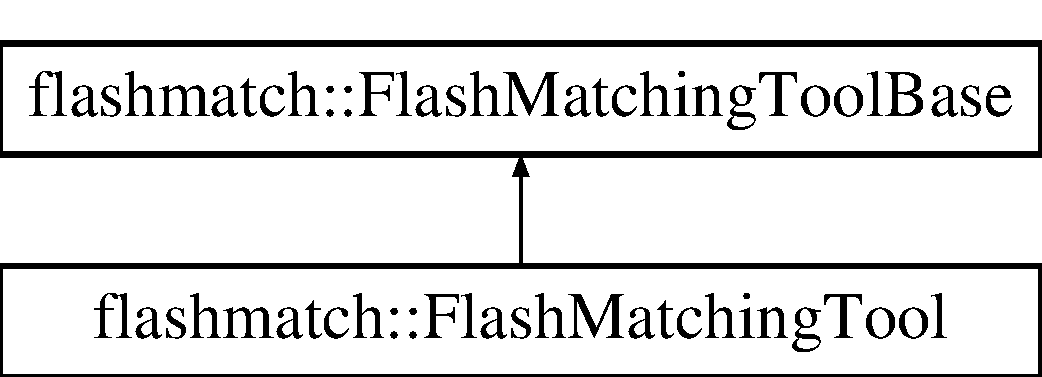
\includegraphics[height=2.000000cm]{classflashmatch_1_1FlashMatchingTool}
\end{center}
\end{figure}
\subsection*{Classes}
\begin{DoxyCompactItemize}
\item 
class \hyperlink{classflashmatch_1_1FlashMatchingTool_1_1FailureMode}{Failure\-Mode}
\begin{DoxyCompactList}\small\item\em A description of the reason the tool couldn't find a neutrino candidate. \end{DoxyCompactList}\item 
class \hyperlink{classflashmatch_1_1FlashMatchingTool_1_1FlashCandidate}{Flash\-Candidate}
\begin{DoxyCompactList}\small\item\em A candidate for the beam flash. \end{DoxyCompactList}\item 
class \hyperlink{classflashmatch_1_1FlashMatchingTool_1_1OutputEvent}{Output\-Event}
\begin{DoxyCompactList}\small\item\em Class to hold information about the event for monitoring. \end{DoxyCompactList}\item 
class \hyperlink{classflashmatch_1_1FlashMatchingTool_1_1SliceCandidate}{Slice\-Candidate}
\begin{DoxyCompactList}\small\item\em A candidate for the target slice. \end{DoxyCompactList}\end{DoxyCompactItemize}
\subsection*{Public Member Functions}
\begin{DoxyCompactItemize}
\item 
\hyperlink{classflashmatch_1_1FlashMatchingTool_a8c6b08ba5404a69ad5fc984eaf8a1eba}{Flash\-Matching\-Tool} (const fhicl\-::\-Parameter\-Set \&pset)
\begin{DoxyCompactList}\small\item\em Default constructor. \end{DoxyCompactList}\item 
\hypertarget{classflashmatch_1_1FlashMatchingTool_a58e2b1ea201c0b8429e1111380b0a108}{void {\bfseries configure} (const fhicl\-::\-Parameter\-Set \&pset)}\label{classflashmatch_1_1FlashMatchingTool_a58e2b1ea201c0b8429e1111380b0a108}

\item 
float \hyperlink{classflashmatch_1_1FlashMatchingTool_aed79e484b39c5d02e84714b45c68bf7f}{Classify\-Slice} (const art\-::\-Event \&evt, const std\-::vector$<$ art\-::\-Ptr$<$ recob\-::\-P\-F\-Particle $>$ $>$ \&pfp\-\_\-v, const std\-::vector$<$ std\-::vector$<$ art\-::\-Ptr$<$ recob\-::\-Space\-Point $>$ $>$ $>$ \&spacepoint\-\_\-v\-\_\-v, const std\-::vector$<$ std\-::vector$<$ art\-::\-Ptr$<$ recob\-::\-Hit $>$ $>$ $>$ \&hit\-\_\-v\-\_\-v, std\-::vector$<$ float $>$ \&recospectrum, std\-::vector$<$ float $>$ \&hypospectrum)
\begin{DoxyCompactList}\small\item\em Classify slices as neutrino or cosmic. \end{DoxyCompactList}\item 
\hypertarget{classflashmatch_1_1FlashMatchingTool_a576990a409d28ed7526963195df7e55a}{float {\bfseries Classify\-Track} (const art\-::\-Event \&evt, const std\-::vector$<$ art\-::\-Ptr$<$ recob\-::\-Space\-Point $>$ $>$ \&spacepoint\-\_\-v, const std\-::vector$<$ art\-::\-Ptr$<$ recob\-::\-Hit $>$ $>$ \&hit\-\_\-v, std\-::vector$<$ float $>$ \&recospectrum, std\-::vector$<$ float $>$ \&hypospectrum)}\label{classflashmatch_1_1FlashMatchingTool_a576990a409d28ed7526963195df7e55a}

\end{DoxyCompactItemize}
\subsection*{Private Types}
\begin{DoxyCompactItemize}
\item 
\hypertarget{classflashmatch_1_1FlashMatchingTool_a6a9ab4e3315550624ddc72103c2d260c}{typedef std\-::vector\\*
$<$ \hyperlink{classflashmatch_1_1FlashMatchingTool_1_1SliceCandidate}{Slice\-Candidate} $>$ {\bfseries Slice\-Candidate\-Vector}}\label{classflashmatch_1_1FlashMatchingTool_a6a9ab4e3315550624ddc72103c2d260c}

\item 
\hypertarget{classflashmatch_1_1FlashMatchingTool_ae4ca02d264c29ff19c6d32627c4bf852}{typedef std\-::vector\\*
$<$ \hyperlink{classflashmatch_1_1FlashMatchingTool_1_1FlashCandidate}{Flash\-Candidate} $>$ {\bfseries Flash\-Candidate\-Vector}}\label{classflashmatch_1_1FlashMatchingTool_ae4ca02d264c29ff19c6d32627c4bf852}

\end{DoxyCompactItemize}
\subsection*{Private Member Functions}
\begin{DoxyCompactItemize}
\item 
void \hyperlink{classflashmatch_1_1FlashMatchingTool_a68229bfc94d94e91513fefe60a3b43d6}{Get\-Flash\-Candidates} (const art\-::\-Event \&event, Flash\-Candidate\-Vector \&flash\-Candidates)
\begin{DoxyCompactList}\small\item\em Get the candidate flashes in the event. \end{DoxyCompactList}\item 
\hyperlink{classflashmatch_1_1FlashMatchingTool_1_1FlashCandidate}{Flash\-Candidate} \& \hyperlink{classflashmatch_1_1FlashMatchingTool_a55eb0441a37240344fc893857aabda28}{Get\-Beam\-Flash} (Flash\-Candidate\-Vector \&flash\-Candidates)
\item 
float \hyperlink{classflashmatch_1_1FlashMatchingTool_a64dcefa0f3f8e95d51dcb0aadbc711c8}{Get\-Slice\-Score} (\hyperlink{classflashmatch_1_1FlashMatchingTool_1_1FlashCandidate}{Flash\-Candidate} \&beam\-Flash, \hyperlink{classflashmatch_1_1FlashMatchingTool_1_1SliceCandidate}{Slice\-Candidate} \&slice)
\begin{DoxyCompactList}\small\item\em get the score \end{DoxyCompactList}\end{DoxyCompactItemize}
\subsection*{Private Attributes}
\begin{DoxyCompactItemize}
\item 
\hypertarget{classflashmatch_1_1FlashMatchingTool_a1d8717c68408b4b6bcada1d833f52b85}{std\-::string \hyperlink{classflashmatch_1_1FlashMatchingTool_a1d8717c68408b4b6bcada1d833f52b85}{m\-\_\-flash\-Label}}\label{classflashmatch_1_1FlashMatchingTool_a1d8717c68408b4b6bcada1d833f52b85}

\begin{DoxyCompactList}\small\item\em The label of the flash producer. \end{DoxyCompactList}\item 
\hypertarget{classflashmatch_1_1FlashMatchingTool_a268e4c99f49178112c76b0fd4f5dc83e}{std\-::string \hyperlink{classflashmatch_1_1FlashMatchingTool_a268e4c99f49178112c76b0fd4f5dc83e}{m\-\_\-pandora\-Label}}\label{classflashmatch_1_1FlashMatchingTool_a268e4c99f49178112c76b0fd4f5dc83e}

\begin{DoxyCompactList}\small\item\em The label of the all\-Outcomes pandora producer. \end{DoxyCompactList}\item 
\hypertarget{classflashmatch_1_1FlashMatchingTool_a33272b2692b9eee1ee1f5af82696e558}{float \hyperlink{classflashmatch_1_1FlashMatchingTool_a33272b2692b9eee1ee1f5af82696e558}{m\-\_\-beam\-Window\-Start}}\label{classflashmatch_1_1FlashMatchingTool_a33272b2692b9eee1ee1f5af82696e558}

\begin{DoxyCompactList}\small\item\em The start time of the beam window. \end{DoxyCompactList}\item 
\hypertarget{classflashmatch_1_1FlashMatchingTool_a8a7cc0d75c962df7d5bf20cc1edccde2}{float \hyperlink{classflashmatch_1_1FlashMatchingTool_a8a7cc0d75c962df7d5bf20cc1edccde2}{m\-\_\-beam\-Window\-End}}\label{classflashmatch_1_1FlashMatchingTool_a8a7cc0d75c962df7d5bf20cc1edccde2}

\begin{DoxyCompactList}\small\item\em The end time of the beam window. \end{DoxyCompactList}\item 
\hypertarget{classflashmatch_1_1FlashMatchingTool_ab6bfd0f0b1d32f1d647d978963ffcfea}{float \hyperlink{classflashmatch_1_1FlashMatchingTool_ab6bfd0f0b1d32f1d647d978963ffcfea}{m\-\_\-min\-Beam\-Flash\-P\-E}}\label{classflashmatch_1_1FlashMatchingTool_ab6bfd0f0b1d32f1d647d978963ffcfea}

\begin{DoxyCompactList}\small\item\em The minimum number of photoelectrons required to consider a flash as the beam flash. \end{DoxyCompactList}\item 
\hypertarget{classflashmatch_1_1FlashMatchingTool_ad4ea54d8957415c895afdd3575dda380}{float \hyperlink{classflashmatch_1_1FlashMatchingTool_ad4ea54d8957415c895afdd3575dda380}{m\-\_\-xcl\-Coef}}\label{classflashmatch_1_1FlashMatchingTool_ad4ea54d8957415c895afdd3575dda380}

\begin{DoxyCompactList}\small\item\em m\-\_\-xcl\-Coef$\ast$log10(charge\-To\-Light\-Ratio)-\/ center\-X \end{DoxyCompactList}\item 
\hypertarget{classflashmatch_1_1FlashMatchingTool_a859f9d3405d8f5bae13b3927e193ab91}{float \hyperlink{classflashmatch_1_1FlashMatchingTool_a859f9d3405d8f5bae13b3927e193ab91}{m\-\_\-max\-Delta\-Y}}\label{classflashmatch_1_1FlashMatchingTool_a859f9d3405d8f5bae13b3927e193ab91}

\begin{DoxyCompactList}\small\item\em The maximum difference in Y between the beam flash center and the weighted charge center. \end{DoxyCompactList}\item 
\hypertarget{classflashmatch_1_1FlashMatchingTool_a8b66b2458157a6216b83200359b6bb17}{float \hyperlink{classflashmatch_1_1FlashMatchingTool_a8b66b2458157a6216b83200359b6bb17}{m\-\_\-max\-Delta\-Z}}\label{classflashmatch_1_1FlashMatchingTool_a8b66b2458157a6216b83200359b6bb17}

\begin{DoxyCompactList}\small\item\em The maximum difference in Z between the beam flash center and the weighted charge center. \end{DoxyCompactList}\item 
\hypertarget{classflashmatch_1_1FlashMatchingTool_a255b27c95bb3d2954482e3fdc8cf3e79}{float \hyperlink{classflashmatch_1_1FlashMatchingTool_a255b27c95bb3d2954482e3fdc8cf3e79}{m\-\_\-max\-Delta\-Y\-Sigma}}\label{classflashmatch_1_1FlashMatchingTool_a255b27c95bb3d2954482e3fdc8cf3e79}

\begin{DoxyCompactList}\small\item\em As for max\-Delta\-Y, but measured in units of the flash width in Y. \end{DoxyCompactList}\item 
\hypertarget{classflashmatch_1_1FlashMatchingTool_aa5460134c0dbb87c67ca199a0ddb67ac}{float \hyperlink{classflashmatch_1_1FlashMatchingTool_aa5460134c0dbb87c67ca199a0ddb67ac}{m\-\_\-max\-Delta\-Z\-Sigma}}\label{classflashmatch_1_1FlashMatchingTool_aa5460134c0dbb87c67ca199a0ddb67ac}

\begin{DoxyCompactList}\small\item\em As for max\-Delta\-Z, but measured in units of the flash width in Z. \end{DoxyCompactList}\item 
\hypertarget{classflashmatch_1_1FlashMatchingTool_ab4b223f8fca98bb3e6372762228b3065}{float \hyperlink{classflashmatch_1_1FlashMatchingTool_ab4b223f8fca98bb3e6372762228b3065}{m\-\_\-min\-Charge\-To\-Light\-Ratio}}\label{classflashmatch_1_1FlashMatchingTool_ab4b223f8fca98bb3e6372762228b3065}

\begin{DoxyCompactList}\small\item\em The minimum ratio between the total charge and the total P\-E. \end{DoxyCompactList}\item 
\hypertarget{classflashmatch_1_1FlashMatchingTool_a2f5ba137ceabb7e78a992db8f66ff0ad}{float \hyperlink{classflashmatch_1_1FlashMatchingTool_a2f5ba137ceabb7e78a992db8f66ff0ad}{m\-\_\-max\-Charge\-To\-Light\-Ratio}}\label{classflashmatch_1_1FlashMatchingTool_a2f5ba137ceabb7e78a992db8f66ff0ad}

\begin{DoxyCompactList}\small\item\em The maximum ratio between the total charge and the total P\-E. \end{DoxyCompactList}\item 
\hypertarget{classflashmatch_1_1FlashMatchingTool_a89d4a6c3dae8a3a8aa0db8c0c9a0cb21}{float \hyperlink{classflashmatch_1_1FlashMatchingTool_a89d4a6c3dae8a3a8aa0db8c0c9a0cb21}{m\-\_\-charge\-To\-N\-Photons\-Track}}\label{classflashmatch_1_1FlashMatchingTool_a89d4a6c3dae8a3a8aa0db8c0c9a0cb21}

\begin{DoxyCompactList}\small\item\em The conversion factor between charge and number of photons for tracks. \end{DoxyCompactList}\item 
\hypertarget{classflashmatch_1_1FlashMatchingTool_ab914c01e557cee0b0dd0c461759e7135}{float \hyperlink{classflashmatch_1_1FlashMatchingTool_ab914c01e557cee0b0dd0c461759e7135}{m\-\_\-charge\-To\-N\-Photons\-Shower}}\label{classflashmatch_1_1FlashMatchingTool_ab914c01e557cee0b0dd0c461759e7135}

\begin{DoxyCompactList}\small\item\em The conversion factor between charge and number of photons for showers. \end{DoxyCompactList}\item 
\hypertarget{classflashmatch_1_1FlashMatchingTool_a11b980eee1a9ecbe15663af51885846d}{flashana\-::\-Flash\-Match\-Manager \hyperlink{classflashmatch_1_1FlashMatchingTool_a11b980eee1a9ecbe15663af51885846d}{m\-\_\-flash\-Match\-Manager}}\label{classflashmatch_1_1FlashMatchingTool_a11b980eee1a9ecbe15663af51885846d}

\begin{DoxyCompactList}\small\item\em The flash match manager. \end{DoxyCompactList}\item 
\hypertarget{classflashmatch_1_1FlashMatchingTool_a4463e9c421fa26d464b037b125e0a11d}{bool \hyperlink{classflashmatch_1_1FlashMatchingTool_a4463e9c421fa26d464b037b125e0a11d}{m\-\_\-should\-Write\-To\-File}}\label{classflashmatch_1_1FlashMatchingTool_a4463e9c421fa26d464b037b125e0a11d}

\begin{DoxyCompactList}\small\item\em If we should write interesting information to a root file. \end{DoxyCompactList}\item 
\hypertarget{classflashmatch_1_1FlashMatchingTool_a6a48a0c7ba51c6383080aec264c41ea0}{bool \hyperlink{classflashmatch_1_1FlashMatchingTool_a6a48a0c7ba51c6383080aec264c41ea0}{m\-\_\-has\-M\-C\-Neutrino}}\label{classflashmatch_1_1FlashMatchingTool_a6a48a0c7ba51c6383080aec264c41ea0}

\begin{DoxyCompactList}\small\item\em If there is an M\-C neutrino we can use to get truth information. \end{DoxyCompactList}\item 
\hypertarget{classflashmatch_1_1FlashMatchingTool_af55fe95515811281eaabe0b127b73e10}{int \hyperlink{classflashmatch_1_1FlashMatchingTool_af55fe95515811281eaabe0b127b73e10}{m\-\_\-nu\-Interaction\-Type}}\label{classflashmatch_1_1FlashMatchingTool_af55fe95515811281eaabe0b127b73e10}

\begin{DoxyCompactList}\small\item\em The interaction type code from M\-C\-Truth. \end{DoxyCompactList}\item 
\hypertarget{classflashmatch_1_1FlashMatchingTool_af149140ded5d54d8a16d57bcb7bcef9f}{int \hyperlink{classflashmatch_1_1FlashMatchingTool_af149140ded5d54d8a16d57bcb7bcef9f}{m\-\_\-nu\-C\-C\-N\-C}}\label{classflashmatch_1_1FlashMatchingTool_af149140ded5d54d8a16d57bcb7bcef9f}

\begin{DoxyCompactList}\small\item\em Charged current or neutral current? \end{DoxyCompactList}\item 
\hypertarget{classflashmatch_1_1FlashMatchingTool_a8fd18741587d821f70572d0accc70def}{float \hyperlink{classflashmatch_1_1FlashMatchingTool_a8fd18741587d821f70572d0accc70def}{m\-\_\-nu\-Energy}}\label{classflashmatch_1_1FlashMatchingTool_a8fd18741587d821f70572d0accc70def}

\begin{DoxyCompactList}\small\item\em The true neutrino energy. \end{DoxyCompactList}\item 
\hypertarget{classflashmatch_1_1FlashMatchingTool_a9b34756c62ad017bee3da0c5d19330d9}{float \hyperlink{classflashmatch_1_1FlashMatchingTool_a9b34756c62ad017bee3da0c5d19330d9}{m\-\_\-lepton\-Energy}}\label{classflashmatch_1_1FlashMatchingTool_a9b34756c62ad017bee3da0c5d19330d9}

\begin{DoxyCompactList}\small\item\em The true energy of the lepton coming from the C\-C interaction. \end{DoxyCompactList}\item 
\hypertarget{classflashmatch_1_1FlashMatchingTool_abb21852617cec0a27cda3462a0a11bff}{float \hyperlink{classflashmatch_1_1FlashMatchingTool_abb21852617cec0a27cda3462a0a11bff}{m\-\_\-nu\-Vertex\-X}}\label{classflashmatch_1_1FlashMatchingTool_abb21852617cec0a27cda3462a0a11bff}

\begin{DoxyCompactList}\small\item\em The true neutrino vertex X position. \end{DoxyCompactList}\item 
\hypertarget{classflashmatch_1_1FlashMatchingTool_a356775f0a1f6304ac89ed0d53d671f51}{float \hyperlink{classflashmatch_1_1FlashMatchingTool_a356775f0a1f6304ac89ed0d53d671f51}{m\-\_\-nu\-Vertex\-Y}}\label{classflashmatch_1_1FlashMatchingTool_a356775f0a1f6304ac89ed0d53d671f51}

\begin{DoxyCompactList}\small\item\em The true neutrino vertex Y position. \end{DoxyCompactList}\item 
\hypertarget{classflashmatch_1_1FlashMatchingTool_a085ef14efb0bbfd5d6a2daa902f79c64}{float \hyperlink{classflashmatch_1_1FlashMatchingTool_a085ef14efb0bbfd5d6a2daa902f79c64}{m\-\_\-nu\-Vertex\-Z}}\label{classflashmatch_1_1FlashMatchingTool_a085ef14efb0bbfd5d6a2daa902f79c64}

\begin{DoxyCompactList}\small\item\em The true neutrino vertex Z position. \end{DoxyCompactList}\item 
\hypertarget{classflashmatch_1_1FlashMatchingTool_a6ea1d944847273ae6ce6f0ef5fd82497}{float \hyperlink{classflashmatch_1_1FlashMatchingTool_a6ea1d944847273ae6ce6f0ef5fd82497}{m\-\_\-nu\-Time}}\label{classflashmatch_1_1FlashMatchingTool_a6ea1d944847273ae6ce6f0ef5fd82497}

\begin{DoxyCompactList}\small\item\em The time of the true neutrino interaction. \end{DoxyCompactList}\item 
\hypertarget{classflashmatch_1_1FlashMatchingTool_abeeea00e4d39a887fb13874b788288c5}{int \hyperlink{classflashmatch_1_1FlashMatchingTool_abeeea00e4d39a887fb13874b788288c5}{m\-\_\-nu\-Pdg\-Code}}\label{classflashmatch_1_1FlashMatchingTool_abeeea00e4d39a887fb13874b788288c5}

\begin{DoxyCompactList}\small\item\em The true neutrino pdg code. \end{DoxyCompactList}\item 
\hypertarget{classflashmatch_1_1FlashMatchingTool_a7ecd3035c9f9871021e0eed80db108e7}{std\-::string \hyperlink{classflashmatch_1_1FlashMatchingTool_a7ecd3035c9f9871021e0eed80db108e7}{m\-\_\-truth\-Label}}\label{classflashmatch_1_1FlashMatchingTool_a7ecd3035c9f9871021e0eed80db108e7}

\begin{DoxyCompactList}\small\item\em The M\-C\-Truth producer label. \end{DoxyCompactList}\item 
\hypertarget{classflashmatch_1_1FlashMatchingTool_ab68ae36a24edb32725cc8f6b5884cc93}{std\-::string \hyperlink{classflashmatch_1_1FlashMatchingTool_ab68ae36a24edb32725cc8f6b5884cc93}{m\-\_\-mc\-Particle\-Label}}\label{classflashmatch_1_1FlashMatchingTool_ab68ae36a24edb32725cc8f6b5884cc93}

\begin{DoxyCompactList}\small\item\em The M\-C\-Particle producer label. \end{DoxyCompactList}\item 
\hypertarget{classflashmatch_1_1FlashMatchingTool_a8dff6789389dc7519c006616d1dc80ea}{std\-::string \hyperlink{classflashmatch_1_1FlashMatchingTool_a8dff6789389dc7519c006616d1dc80ea}{m\-\_\-hit\-Label}}\label{classflashmatch_1_1FlashMatchingTool_a8dff6789389dc7519c006616d1dc80ea}

\begin{DoxyCompactList}\small\item\em The Hit producer label. \end{DoxyCompactList}\item 
\hypertarget{classflashmatch_1_1FlashMatchingTool_aab819e6949faa62cc05cc990f062db9b}{std\-::string \hyperlink{classflashmatch_1_1FlashMatchingTool_aab819e6949faa62cc05cc990f062db9b}{m\-\_\-backtrack\-Label}}\label{classflashmatch_1_1FlashMatchingTool_aab819e6949faa62cc05cc990f062db9b}

\begin{DoxyCompactList}\small\item\em The Hit -\/$>$ M\-C\-Particle producer label. \end{DoxyCompactList}\item 
\hypertarget{classflashmatch_1_1FlashMatchingTool_a17f8d293d8a8a47a3a18782c1975cca5}{\hyperlink{classflashmatch_1_1FlashMatchingTool_1_1OutputEvent}{Output\-Event} \hyperlink{classflashmatch_1_1FlashMatchingTool_a17f8d293d8a8a47a3a18782c1975cca5}{m\-\_\-output\-Event}}\label{classflashmatch_1_1FlashMatchingTool_a17f8d293d8a8a47a3a18782c1975cca5}

\begin{DoxyCompactList}\small\item\em The output event whose address is used by the output branch. \end{DoxyCompactList}\item 
\hypertarget{classflashmatch_1_1FlashMatchingTool_a5143114bf5396507981d5beb51cd19ff}{\hyperlink{classflashmatch_1_1FlashMatchingTool_1_1FlashCandidate}{Flash\-Candidate} \hyperlink{classflashmatch_1_1FlashMatchingTool_a5143114bf5396507981d5beb51cd19ff}{m\-\_\-output\-Flash}}\label{classflashmatch_1_1FlashMatchingTool_a5143114bf5396507981d5beb51cd19ff}

\begin{DoxyCompactList}\small\item\em The output flash whose address is used by the output branch. \end{DoxyCompactList}\item 
\hypertarget{classflashmatch_1_1FlashMatchingTool_a1cfed4e60733015c5db55b7683f83fc7}{\hyperlink{classflashmatch_1_1FlashMatchingTool_1_1SliceCandidate}{Slice\-Candidate} \hyperlink{classflashmatch_1_1FlashMatchingTool_a1cfed4e60733015c5db55b7683f83fc7}{m\-\_\-output\-Slice}}\label{classflashmatch_1_1FlashMatchingTool_a1cfed4e60733015c5db55b7683f83fc7}

\begin{DoxyCompactList}\small\item\em The output slice whose address is used by the output branch. \end{DoxyCompactList}\item 
\hypertarget{classflashmatch_1_1FlashMatchingTool_a34a8387456b15a105daac14517040d4d}{T\-Tree $\ast$ \hyperlink{classflashmatch_1_1FlashMatchingTool_a34a8387456b15a105daac14517040d4d}{m\-\_\-p\-Flash\-Tree}}\label{classflashmatch_1_1FlashMatchingTool_a34a8387456b15a105daac14517040d4d}

\begin{DoxyCompactList}\small\item\em The flash tree. \end{DoxyCompactList}\end{DoxyCompactItemize}


\subsection{Constructor \& Destructor Documentation}
\hypertarget{classflashmatch_1_1FlashMatchingTool_a8c6b08ba5404a69ad5fc984eaf8a1eba}{\index{flashmatch\-::\-Flash\-Matching\-Tool@{flashmatch\-::\-Flash\-Matching\-Tool}!Flash\-Matching\-Tool@{Flash\-Matching\-Tool}}
\index{Flash\-Matching\-Tool@{Flash\-Matching\-Tool}!flashmatch::FlashMatchingTool@{flashmatch\-::\-Flash\-Matching\-Tool}}
\subsubsection[{Flash\-Matching\-Tool}]{\setlength{\rightskip}{0pt plus 5cm}flashmatch\-::\-Flash\-Matching\-Tool\-::\-Flash\-Matching\-Tool (
\begin{DoxyParamCaption}
\item[{const fhicl\-::\-Parameter\-Set \&}]{pset}
\end{DoxyParamCaption}
)\hspace{0.3cm}{\ttfamily [inline]}, {\ttfamily [explicit]}}}\label{classflashmatch_1_1FlashMatchingTool_a8c6b08ba5404a69ad5fc984eaf8a1eba}


Default constructor. 


\begin{DoxyParams}{Parameters}
{\em pset} & F\-Hi\-C\-L parameter set \\
\hline
\end{DoxyParams}


\subsection{Member Function Documentation}
\hypertarget{classflashmatch_1_1FlashMatchingTool_aed79e484b39c5d02e84714b45c68bf7f}{\index{flashmatch\-::\-Flash\-Matching\-Tool@{flashmatch\-::\-Flash\-Matching\-Tool}!Classify\-Slice@{Classify\-Slice}}
\index{Classify\-Slice@{Classify\-Slice}!flashmatch::FlashMatchingTool@{flashmatch\-::\-Flash\-Matching\-Tool}}
\subsubsection[{Classify\-Slice}]{\setlength{\rightskip}{0pt plus 5cm}float flashmatch\-::\-Flash\-Matching\-Tool\-::\-Classify\-Slice (
\begin{DoxyParamCaption}
\item[{const art\-::\-Event \&}]{evt, }
\item[{const std\-::vector$<$ art\-::\-Ptr$<$ recob\-::\-P\-F\-Particle $>$ $>$ \&}]{pfp\-\_\-v, }
\item[{const std\-::vector$<$ std\-::vector$<$ art\-::\-Ptr$<$ recob\-::\-Space\-Point $>$ $>$ $>$ \&}]{spacepoint\-\_\-v\-\_\-v, }
\item[{const std\-::vector$<$ std\-::vector$<$ art\-::\-Ptr$<$ recob\-::\-Hit $>$ $>$ $>$ \&}]{hit\-\_\-v\-\_\-v, }
\item[{std\-::vector$<$ float $>$ \&}]{recospectrum, }
\item[{std\-::vector$<$ float $>$ \&}]{hypospectrum}
\end{DoxyParamCaption}
)\hspace{0.3cm}{\ttfamily [virtual]}}}\label{classflashmatch_1_1FlashMatchingTool_aed79e484b39c5d02e84714b45c68bf7f}


Classify slices as neutrino or cosmic. 


\begin{DoxyParams}{Parameters}
{\em slices} & the input vector of slices to classify \\
\hline
{\em evt} & the art event \\
\hline
\end{DoxyParams}


Implements \hyperlink{classflashmatch_1_1FlashMatchingToolBase_a79d9ba4fe96a0b887631c8ae62f7cbcd}{flashmatch\-::\-Flash\-Matching\-Tool\-Base}.

\hypertarget{classflashmatch_1_1FlashMatchingTool_a55eb0441a37240344fc893857aabda28}{\index{flashmatch\-::\-Flash\-Matching\-Tool@{flashmatch\-::\-Flash\-Matching\-Tool}!Get\-Beam\-Flash@{Get\-Beam\-Flash}}
\index{Get\-Beam\-Flash@{Get\-Beam\-Flash}!flashmatch::FlashMatchingTool@{flashmatch\-::\-Flash\-Matching\-Tool}}
\subsubsection[{Get\-Beam\-Flash}]{\setlength{\rightskip}{0pt plus 5cm}{\bf Flash\-Candidate}\& flashmatch\-::\-Flash\-Matching\-Tool\-::\-Get\-Beam\-Flash (
\begin{DoxyParamCaption}
\item[{Flash\-Candidate\-Vector \&}]{flash\-Candidates}
\end{DoxyParamCaption}
)\hspace{0.3cm}{\ttfamily [inline]}, {\ttfamily [private]}}}\label{classflashmatch_1_1FlashMatchingTool_a55eb0441a37240344fc893857aabda28}
Try to find the brightest flash with sufficent photoelectons that is in time with the beam


\begin{DoxyParams}{Parameters}
{\em flash\-Candidates} & the input vector of slice candidates\\
\hline
\end{DoxyParams}
\begin{DoxyReturn}{Returns}
the beam flash 
\end{DoxyReturn}
\hypertarget{classflashmatch_1_1FlashMatchingTool_a68229bfc94d94e91513fefe60a3b43d6}{\index{flashmatch\-::\-Flash\-Matching\-Tool@{flashmatch\-::\-Flash\-Matching\-Tool}!Get\-Flash\-Candidates@{Get\-Flash\-Candidates}}
\index{Get\-Flash\-Candidates@{Get\-Flash\-Candidates}!flashmatch::FlashMatchingTool@{flashmatch\-::\-Flash\-Matching\-Tool}}
\subsubsection[{Get\-Flash\-Candidates}]{\setlength{\rightskip}{0pt plus 5cm}void flashmatch\-::\-Flash\-Matching\-Tool\-::\-Get\-Flash\-Candidates (
\begin{DoxyParamCaption}
\item[{const art\-::\-Event \&}]{event, }
\item[{Flash\-Candidate\-Vector \&}]{flash\-Candidates}
\end{DoxyParamCaption}
)\hspace{0.3cm}{\ttfamily [inline]}, {\ttfamily [private]}}}\label{classflashmatch_1_1FlashMatchingTool_a68229bfc94d94e91513fefe60a3b43d6}


Get the candidate flashes in the event. 


\begin{DoxyParams}{Parameters}
{\em event} & the art event \\
\hline
{\em flash\-Candidates} & the output vector of flash candidates \\
\hline
\end{DoxyParams}
\hypertarget{classflashmatch_1_1FlashMatchingTool_a64dcefa0f3f8e95d51dcb0aadbc711c8}{\index{flashmatch\-::\-Flash\-Matching\-Tool@{flashmatch\-::\-Flash\-Matching\-Tool}!Get\-Slice\-Score@{Get\-Slice\-Score}}
\index{Get\-Slice\-Score@{Get\-Slice\-Score}!flashmatch::FlashMatchingTool@{flashmatch\-::\-Flash\-Matching\-Tool}}
\subsubsection[{Get\-Slice\-Score}]{\setlength{\rightskip}{0pt plus 5cm}float flashmatch\-::\-Flash\-Matching\-Tool\-::\-Get\-Slice\-Score (
\begin{DoxyParamCaption}
\item[{{\bf Flash\-Candidate} \&}]{beam\-Flash, }
\item[{{\bf Slice\-Candidate} \&}]{slice}
\end{DoxyParamCaption}
)\hspace{0.3cm}{\ttfamily [inline]}, {\ttfamily [private]}}}\label{classflashmatch_1_1FlashMatchingTool_a64dcefa0f3f8e95d51dcb0aadbc711c8}


get the score 


\begin{DoxyParams}{Parameters}
{\em beam\-Flash} & the beam flash \\
\hline
{\em slice\-Candidates} & the neutrino slice candidates \\
\hline
\end{DoxyParams}


The documentation for this class was generated from the following file\-:\begin{DoxyCompactItemize}
\item 
/home/travis/build/ubneutrinos/searchingfornues/\-Flash\-Matching/Flash\-Matching\-Tool\-\_\-tool.\-cc\end{DoxyCompactItemize}

\hypertarget{classflashmatch_1_1FlashMatchingToolBase}{\section{flashmatch\-:\-:Flash\-Matching\-Tool\-Base Class Reference}
\label{classflashmatch_1_1FlashMatchingToolBase}\index{flashmatch\-::\-Flash\-Matching\-Tool\-Base@{flashmatch\-::\-Flash\-Matching\-Tool\-Base}}
}


Neutrino I\-D tool that selects the most likely neutrino slice using P\-M\-T information.  




{\ttfamily \#include $<$Flash\-Matching\-Tool\-Base\-\_\-tool.\-h$>$}

Inheritance diagram for flashmatch\-:\-:Flash\-Matching\-Tool\-Base\-:\begin{figure}[H]
\begin{center}
\leavevmode
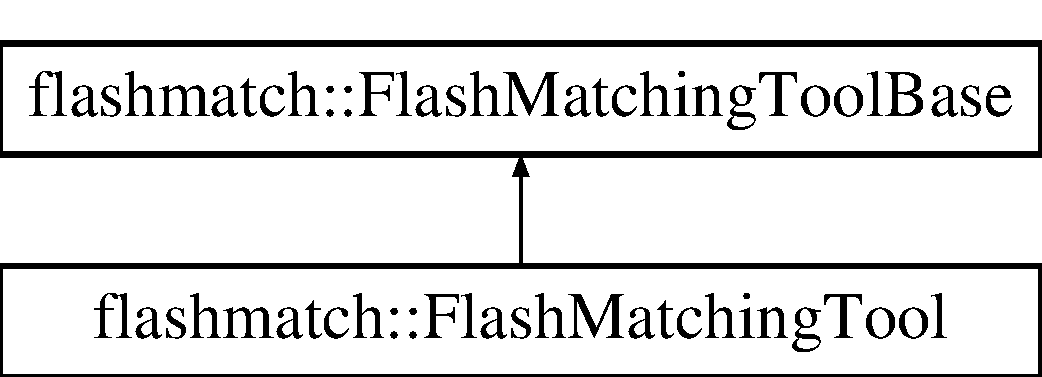
\includegraphics[height=2.000000cm]{classflashmatch_1_1FlashMatchingToolBase}
\end{center}
\end{figure}
\subsection*{Public Member Functions}
\begin{DoxyCompactItemize}
\item 
\hypertarget{classflashmatch_1_1FlashMatchingToolBase_a8133f8cf2289dd17d0a05ba2a3c02da4}{float {\bfseries Classify\-Slice} ()}\label{classflashmatch_1_1FlashMatchingToolBase_a8133f8cf2289dd17d0a05ba2a3c02da4}

\item 
virtual float \hyperlink{classflashmatch_1_1FlashMatchingToolBase_a79d9ba4fe96a0b887631c8ae62f7cbcd}{Classify\-Slice} (const art\-::\-Event \&evt, const std\-::vector$<$ art\-::\-Ptr$<$ recob\-::\-P\-F\-Particle $>$ $>$ \&pfp\-\_\-v, const std\-::vector$<$ std\-::vector$<$ art\-::\-Ptr$<$ recob\-::\-Space\-Point $>$ $>$ $>$ \&spacepoint\-\_\-v\-\_\-v, const std\-::vector$<$ std\-::vector$<$ art\-::\-Ptr$<$ recob\-::\-Hit $>$ $>$ $>$ \&hit\-\_\-v\-\_\-v, std\-::vector$<$ float $>$ \&recospectrum, std\-::vector$<$ float $>$ \&hypospectrum)=0
\begin{DoxyCompactList}\small\item\em Classify slices as neutrino or cosmic. \end{DoxyCompactList}\item 
\hypertarget{classflashmatch_1_1FlashMatchingToolBase_a3fc65b46bbcebf7d47ead748ef6f5b01}{virtual float {\bfseries Classify\-Track} (const art\-::\-Event \&evt, const std\-::vector$<$ art\-::\-Ptr$<$ recob\-::\-Space\-Point $>$ $>$ \&spacepoint\-\_\-v, const std\-::vector$<$ art\-::\-Ptr$<$ recob\-::\-Hit $>$ $>$ \&hit\-\_\-v, std\-::vector$<$ float $>$ \&recospectrum, std\-::vector$<$ float $>$ \&hypospectrum)=0}\label{classflashmatch_1_1FlashMatchingToolBase_a3fc65b46bbcebf7d47ead748ef6f5b01}

\end{DoxyCompactItemize}


\subsection{Detailed Description}
Neutrino I\-D tool that selects the most likely neutrino slice using P\-M\-T information. 

\subsection{Member Function Documentation}
\hypertarget{classflashmatch_1_1FlashMatchingToolBase_a79d9ba4fe96a0b887631c8ae62f7cbcd}{\index{flashmatch\-::\-Flash\-Matching\-Tool\-Base@{flashmatch\-::\-Flash\-Matching\-Tool\-Base}!Classify\-Slice@{Classify\-Slice}}
\index{Classify\-Slice@{Classify\-Slice}!flashmatch::FlashMatchingToolBase@{flashmatch\-::\-Flash\-Matching\-Tool\-Base}}
\subsubsection[{Classify\-Slice}]{\setlength{\rightskip}{0pt plus 5cm}virtual float flashmatch\-::\-Flash\-Matching\-Tool\-Base\-::\-Classify\-Slice (
\begin{DoxyParamCaption}
\item[{const art\-::\-Event \&}]{evt, }
\item[{const std\-::vector$<$ art\-::\-Ptr$<$ recob\-::\-P\-F\-Particle $>$ $>$ \&}]{pfp\-\_\-v, }
\item[{const std\-::vector$<$ std\-::vector$<$ art\-::\-Ptr$<$ recob\-::\-Space\-Point $>$ $>$ $>$ \&}]{spacepoint\-\_\-v\-\_\-v, }
\item[{const std\-::vector$<$ std\-::vector$<$ art\-::\-Ptr$<$ recob\-::\-Hit $>$ $>$ $>$ \&}]{hit\-\_\-v\-\_\-v, }
\item[{std\-::vector$<$ float $>$ \&}]{recospectrum, }
\item[{std\-::vector$<$ float $>$ \&}]{hypospectrum}
\end{DoxyParamCaption}
)\hspace{0.3cm}{\ttfamily [pure virtual]}}}\label{classflashmatch_1_1FlashMatchingToolBase_a79d9ba4fe96a0b887631c8ae62f7cbcd}


Classify slices as neutrino or cosmic. 


\begin{DoxyParams}{Parameters}
{\em slices} & the input vector of slices to classify \\
\hline
{\em evt} & the art event \\
\hline
\end{DoxyParams}


Implemented in \hyperlink{classflashmatch_1_1FlashMatchingTool_aed79e484b39c5d02e84714b45c68bf7f}{flashmatch\-::\-Flash\-Matching\-Tool}.



The documentation for this class was generated from the following file\-:\begin{DoxyCompactItemize}
\item 
/home/travis/build/ubneutrinos/searchingfornues/\-Flash\-Matching/Flash\-Matching\-Tool\-Base\-\_\-tool.\-h\end{DoxyCompactItemize}

\hypertarget{classMuCSFlashMatch}{\section{Mu\-C\-S\-Flash\-Match Class Reference}
\label{classMuCSFlashMatch}\index{Mu\-C\-S\-Flash\-Match@{Mu\-C\-S\-Flash\-Match}}
}
Inheritance diagram for Mu\-C\-S\-Flash\-Match\-:\begin{figure}[H]
\begin{center}
\leavevmode
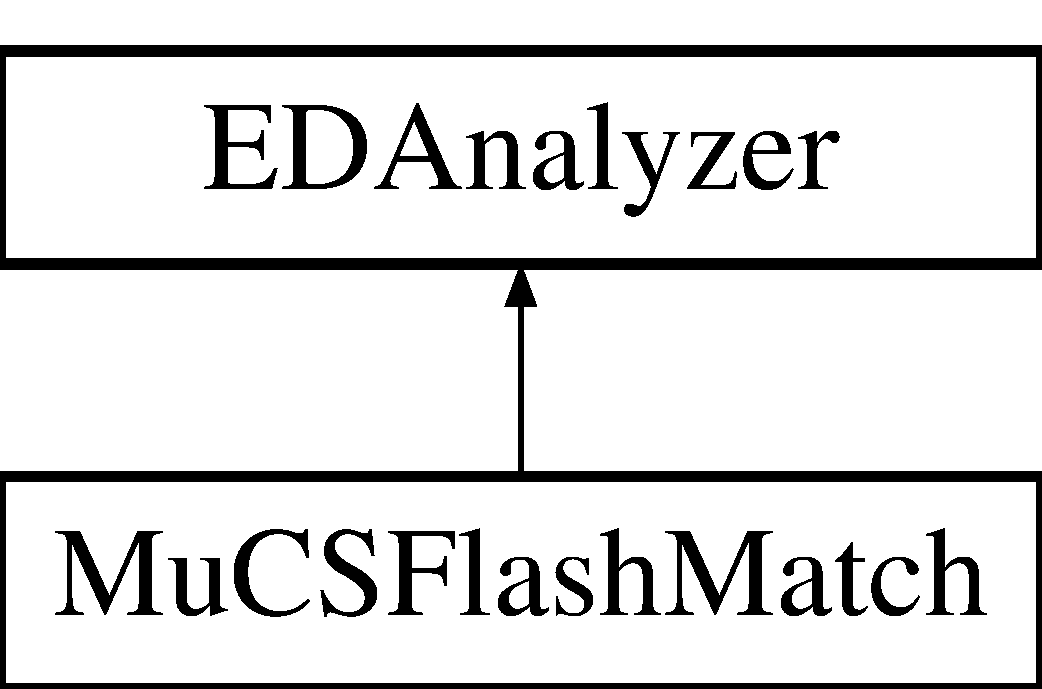
\includegraphics[height=2.000000cm]{classMuCSFlashMatch}
\end{center}
\end{figure}
\subsection*{Public Member Functions}
\begin{DoxyCompactItemize}
\item 
\hypertarget{classMuCSFlashMatch_a62514ddde6a8cf63e3db49649f310468}{{\bfseries Mu\-C\-S\-Flash\-Match} (fhicl\-::\-Parameter\-Set const \&p)}\label{classMuCSFlashMatch_a62514ddde6a8cf63e3db49649f310468}

\item 
\hypertarget{classMuCSFlashMatch_ac77d995753767965120cb78c4942e00c}{{\bfseries Mu\-C\-S\-Flash\-Match} (\hyperlink{classMuCSFlashMatch}{Mu\-C\-S\-Flash\-Match} const \&)=delete}\label{classMuCSFlashMatch_ac77d995753767965120cb78c4942e00c}

\item 
\hypertarget{classMuCSFlashMatch_afced500e296fe05c37e0f1fe112656a9}{{\bfseries Mu\-C\-S\-Flash\-Match} (\hyperlink{classMuCSFlashMatch}{Mu\-C\-S\-Flash\-Match} \&\&)=delete}\label{classMuCSFlashMatch_afced500e296fe05c37e0f1fe112656a9}

\item 
\hypertarget{classMuCSFlashMatch_aa10a3d1be2ea8418188c227d7c4d8864}{\hyperlink{classMuCSFlashMatch}{Mu\-C\-S\-Flash\-Match} \& {\bfseries operator=} (\hyperlink{classMuCSFlashMatch}{Mu\-C\-S\-Flash\-Match} const \&)=delete}\label{classMuCSFlashMatch_aa10a3d1be2ea8418188c227d7c4d8864}

\item 
\hypertarget{classMuCSFlashMatch_a32339a6105ca8917adedc979b7c7e1da}{\hyperlink{classMuCSFlashMatch}{Mu\-C\-S\-Flash\-Match} \& {\bfseries operator=} (\hyperlink{classMuCSFlashMatch}{Mu\-C\-S\-Flash\-Match} \&\&)=delete}\label{classMuCSFlashMatch_a32339a6105ca8917adedc979b7c7e1da}

\item 
\hypertarget{classMuCSFlashMatch_a17c649cc0efeb756d5432933aa6304cb}{void {\bfseries analyze} (art\-::\-Event const \&e) override}\label{classMuCSFlashMatch_a17c649cc0efeb756d5432933aa6304cb}

\item 
\hypertarget{classMuCSFlashMatch_a578dda78eddb4be556e8ddd40b4da5ea}{void {\bfseries begin\-Job} () override}\label{classMuCSFlashMatch_a578dda78eddb4be556e8ddd40b4da5ea}

\item 
\hypertarget{classMuCSFlashMatch_a2318ec9d880d49696596a93848c38e2c}{void {\bfseries end\-Job} () override}\label{classMuCSFlashMatch_a2318ec9d880d49696596a93848c38e2c}

\end{DoxyCompactItemize}
\subsection*{Private Member Functions}
\begin{DoxyCompactItemize}
\item 
\hypertarget{classMuCSFlashMatch_a7eb5d8ee16d0da0844dd029c3ca8e03e}{bool {\bfseries Through\-Going} (const float \&xs, const float \&ys, const float \&zs, const float \&xe, const float \&ye, const float \&ze)}\label{classMuCSFlashMatch_a7eb5d8ee16d0da0844dd029c3ca8e03e}

\end{DoxyCompactItemize}
\subsection*{Private Attributes}
\begin{DoxyCompactItemize}
\item 
\hypertarget{classMuCSFlashMatch_a93159777b3b12a76e8c915b1e577bca4}{T\-Tree $\ast$ {\bfseries \-\_\-tree}}\label{classMuCSFlashMatch_a93159777b3b12a76e8c915b1e577bca4}

\item 
\hypertarget{classMuCSFlashMatch_a153c65fb60d7adb314e9d4942d036390}{float {\bfseries \-\_\-score}}\label{classMuCSFlashMatch_a153c65fb60d7adb314e9d4942d036390}

\item 
\hypertarget{classMuCSFlashMatch_a83d262b8a8ba7ba763fd137f0a26afdb}{int {\bfseries \-\_\-mucs}}\label{classMuCSFlashMatch_a83d262b8a8ba7ba763fd137f0a26afdb}

\item 
\hypertarget{classMuCSFlashMatch_a31d084ffa700c3be29a270a4a9a616fe}{int {\bfseries \-\_\-through}}\label{classMuCSFlashMatch_a31d084ffa700c3be29a270a4a9a616fe}

\item 
\hypertarget{classMuCSFlashMatch_a64f0ee60a2b2259724d9e1f4154d64fc}{T\-Tree $\ast$ {\bfseries \-\_\-evt\-\_\-tree}}\label{classMuCSFlashMatch_a64f0ee60a2b2259724d9e1f4154d64fc}

\item 
\hypertarget{classMuCSFlashMatch_aa38e2faa3f02e5f3aea8c89a8c3afbeb}{int {\bfseries \-\_\-run}}\label{classMuCSFlashMatch_aa38e2faa3f02e5f3aea8c89a8c3afbeb}

\item 
\hypertarget{classMuCSFlashMatch_a9bbc5c1dac231e90fadd96217d6c5769}{int {\bfseries \-\_\-sub}}\label{classMuCSFlashMatch_a9bbc5c1dac231e90fadd96217d6c5769}

\item 
\hypertarget{classMuCSFlashMatch_aba48092457dca63c8945a1192b765587}{int {\bfseries \-\_\-evt}}\label{classMuCSFlashMatch_aba48092457dca63c8945a1192b765587}

\item 
\hypertarget{classMuCSFlashMatch_a086bdb6289764f37faac4dd068357af6}{float {\bfseries \-\_\-best\-\_\-score}}\label{classMuCSFlashMatch_a086bdb6289764f37faac4dd068357af6}

\item 
\hypertarget{classMuCSFlashMatch_a8574cf67b29835c2b985ccbb2a1fc0ef}{float {\bfseries \-\_\-mucs\-\_\-score}}\label{classMuCSFlashMatch_a8574cf67b29835c2b985ccbb2a1fc0ef}

\item 
\hypertarget{classMuCSFlashMatch_a5bf8e15bb3352efd84eb19427e22c667}{std\-::vector$<$ float $>$ {\bfseries \-\_\-score\-\_\-v}}\label{classMuCSFlashMatch_a5bf8e15bb3352efd84eb19427e22c667}

\item 
\hypertarget{classMuCSFlashMatch_a734391610a35cb26469db9420d22e557}{int {\bfseries \-\_\-score\-\_\-mucs\-\_\-idx}}\label{classMuCSFlashMatch_a734391610a35cb26469db9420d22e557}

\item 
\hypertarget{classMuCSFlashMatch_a634f2802c353a87c066aa0098bdb396a}{int {\bfseries \-\_\-best\-\_\-mucs}}\label{classMuCSFlashMatch_a634f2802c353a87c066aa0098bdb396a}

\item 
\hypertarget{classMuCSFlashMatch_a73cae9bc196e8248ff20bb5179c2e07c}{float {\bfseries \-\_\-trk\-\_\-start\-\_\-x}}\label{classMuCSFlashMatch_a73cae9bc196e8248ff20bb5179c2e07c}

\item 
\hypertarget{classMuCSFlashMatch_ae27bbd3758ce1065b5d7126397df6e51}{float {\bfseries \-\_\-trk\-\_\-start\-\_\-y}}\label{classMuCSFlashMatch_ae27bbd3758ce1065b5d7126397df6e51}

\item 
\hypertarget{classMuCSFlashMatch_ad6127cb070a45b0e0e3fc1430969ee4a}{float {\bfseries \-\_\-trk\-\_\-start\-\_\-z}}\label{classMuCSFlashMatch_ad6127cb070a45b0e0e3fc1430969ee4a}

\item 
\hypertarget{classMuCSFlashMatch_aaac8bc4f20184e04b6db6d0e329c9534}{float {\bfseries \-\_\-trk\-\_\-end\-\_\-x}}\label{classMuCSFlashMatch_aaac8bc4f20184e04b6db6d0e329c9534}

\item 
\hypertarget{classMuCSFlashMatch_a98d73685765c3803211170b8ac1e2115}{float {\bfseries \-\_\-trk\-\_\-end\-\_\-y}}\label{classMuCSFlashMatch_a98d73685765c3803211170b8ac1e2115}

\item 
\hypertarget{classMuCSFlashMatch_aa5fff76fe05d7c04cf5f0ff267ef3358}{float {\bfseries \-\_\-trk\-\_\-end\-\_\-z}}\label{classMuCSFlashMatch_aa5fff76fe05d7c04cf5f0ff267ef3358}

\item 
\hypertarget{classMuCSFlashMatch_a336c902544a527f4673c7b82e379392b}{float {\bfseries \-\_\-trk\-\_\-start\-\_\-x\-\_\-mucs}}\label{classMuCSFlashMatch_a336c902544a527f4673c7b82e379392b}

\item 
\hypertarget{classMuCSFlashMatch_a516666ba0806a0ac2494320e9c75ec50}{float {\bfseries \-\_\-trk\-\_\-start\-\_\-y\-\_\-mucs}}\label{classMuCSFlashMatch_a516666ba0806a0ac2494320e9c75ec50}

\item 
\hypertarget{classMuCSFlashMatch_a757af18fa31ba2da2099023c4af05438}{float {\bfseries \-\_\-trk\-\_\-start\-\_\-z\-\_\-mucs}}\label{classMuCSFlashMatch_a757af18fa31ba2da2099023c4af05438}

\item 
\hypertarget{classMuCSFlashMatch_ab8bf9c0a1e791631716ffa579e51a2b0}{float {\bfseries \-\_\-trk\-\_\-end\-\_\-x\-\_\-mucs}}\label{classMuCSFlashMatch_ab8bf9c0a1e791631716ffa579e51a2b0}

\item 
\hypertarget{classMuCSFlashMatch_a6ed4d1d6e27847f17a9536d60cfa849d}{float {\bfseries \-\_\-trk\-\_\-end\-\_\-y\-\_\-mucs}}\label{classMuCSFlashMatch_a6ed4d1d6e27847f17a9536d60cfa849d}

\item 
\hypertarget{classMuCSFlashMatch_a23578eeaa8612076197aea04428a7485}{float {\bfseries \-\_\-trk\-\_\-end\-\_\-z\-\_\-mucs}}\label{classMuCSFlashMatch_a23578eeaa8612076197aea04428a7485}

\item 
\hypertarget{classMuCSFlashMatch_a0f842c11463fffdab3be14c17853185e}{std\-::vector$<$ float $>$ {\bfseries \-\_\-pe\-Spectrum}}\label{classMuCSFlashMatch_a0f842c11463fffdab3be14c17853185e}

\item 
\hypertarget{classMuCSFlashMatch_ac4220bb90ad9debcc818b8273f0fb6c6}{std\-::vector$<$ float $>$ {\bfseries \-\_\-pe\-Hypothesis}}\label{classMuCSFlashMatch_ac4220bb90ad9debcc818b8273f0fb6c6}

\item 
\hypertarget{classMuCSFlashMatch_a7976b1923f812d693d90d8483fc275a3}{std\-::vector$<$ float $>$ {\bfseries \-\_\-pe\-Spectrum\-\_\-mucs}}\label{classMuCSFlashMatch_a7976b1923f812d693d90d8483fc275a3}

\item 
\hypertarget{classMuCSFlashMatch_a41563fc0fde7d884bc82a5843b4bbacb}{std\-::vector$<$ float $>$ {\bfseries \-\_\-pe\-Hypothesis\-\_\-mucs}}\label{classMuCSFlashMatch_a41563fc0fde7d884bc82a5843b4bbacb}

\item 
\hypertarget{classMuCSFlashMatch_a633ec89d3a0296320809bbb81be8cbd8}{std\-::string {\bfseries f\-P\-F\-Pproducer}}\label{classMuCSFlashMatch_a633ec89d3a0296320809bbb81be8cbd8}

\item 
\hypertarget{classMuCSFlashMatch_a2c3c957fd102a157d26b853ba9507058}{std\-::string {\bfseries f\-Trackproducer}}\label{classMuCSFlashMatch_a2c3c957fd102a157d26b853ba9507058}

\item 
\hypertarget{classMuCSFlashMatch_a72e882170ac31de572a22fec62b2c92f}{std\-::string {\bfseries f\-Space\-Pointproducer}}\label{classMuCSFlashMatch_a72e882170ac31de572a22fec62b2c92f}

\item 
\hypertarget{classMuCSFlashMatch_ad581a60155500fe7ddd4c66242575d52}{std\-::string {\bfseries f\-C\-Tagproducer}}\label{classMuCSFlashMatch_ad581a60155500fe7ddd4c66242575d52}

\item 
\hypertarget{classMuCSFlashMatch_ac8212264ca73cfbbb95e8357dce03393}{bool {\bfseries f\-Only\-Tagged}}\label{classMuCSFlashMatch_ac8212264ca73cfbbb95e8357dce03393}

\item 
\hypertarget{classMuCSFlashMatch_ac7d7c6f36ada7a806d24854f30e68c54}{std\-::unique\-\_\-ptr\\*
$<$ \hyperlink{classflashmatch_1_1FlashMatchingToolBase}{flashmatch\-::\-Flash\-Matching\-Tool\-Base} $>$ \hyperlink{classMuCSFlashMatch_ac7d7c6f36ada7a806d24854f30e68c54}{\-\_\-flashmatch\-Tool}}\label{classMuCSFlashMatch_ac7d7c6f36ada7a806d24854f30e68c54}

\begin{DoxyCompactList}\small\item\em The slice id tool. \end{DoxyCompactList}\end{DoxyCompactItemize}


The documentation for this class was generated from the following file\-:\begin{DoxyCompactItemize}
\item 
/home/travis/build/ubneutrinos/searchingfornues/\-Flash\-Matching/Mu\-C\-S\-Flash\-Match\-\_\-module.\-cc\end{DoxyCompactItemize}

\hypertarget{classNeutrinoSelectionFilter}{}\section{Neutrino\+Selection\+Filter Class Reference}
\label{classNeutrinoSelectionFilter}\index{Neutrino\+Selection\+Filter@{Neutrino\+Selection\+Filter}}
Inheritance diagram for Neutrino\+Selection\+Filter\+:\begin{figure}[H]
\begin{center}
\leavevmode
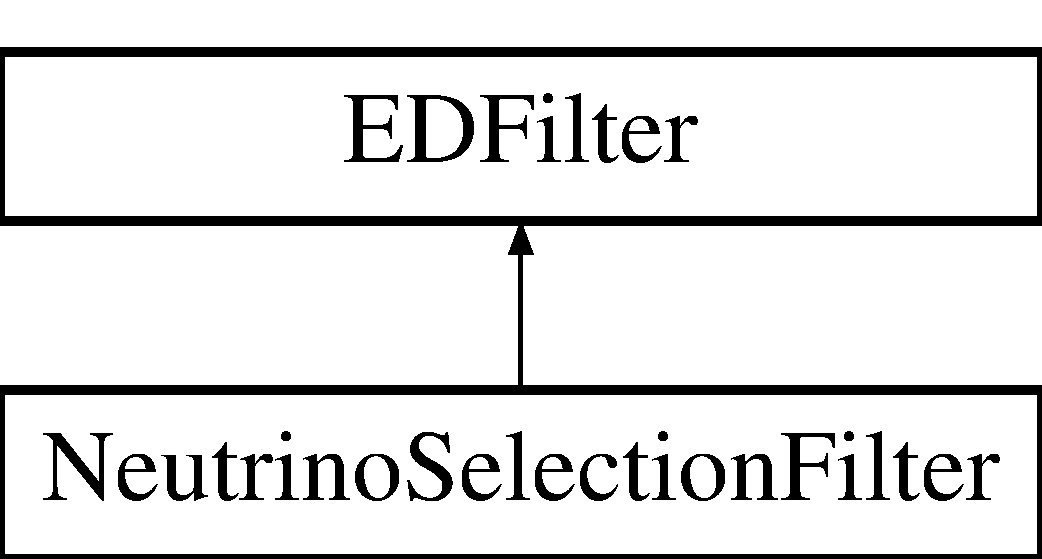
\includegraphics[height=2.000000cm]{classNeutrinoSelectionFilter}
\end{center}
\end{figure}
\subsection*{Public Types}
\begin{DoxyCompactItemize}
\item 
using {\bfseries Proxy\+Pfp\+Coll\+\_\+t} = selection\+::\+Proxy\+Pfp\+Coll\+\_\+t\hypertarget{classNeutrinoSelectionFilter_a7f4b9d53b7df6e6dec6227a60844f112}{}\label{classNeutrinoSelectionFilter_a7f4b9d53b7df6e6dec6227a60844f112}

\item 
using {\bfseries Proxy\+Pfp\+Elem\+\_\+t} = selection\+::\+Proxy\+Pfp\+Elem\+\_\+t\hypertarget{classNeutrinoSelectionFilter_a95a27c35e4604bf0a4feb59231d4e984}{}\label{classNeutrinoSelectionFilter_a95a27c35e4604bf0a4feb59231d4e984}

\end{DoxyCompactItemize}
\subsection*{Public Member Functions}
\begin{DoxyCompactItemize}
\item 
{\bfseries Neutrino\+Selection\+Filter} (fhicl\+::\+Parameter\+Set const \&p)\hypertarget{classNeutrinoSelectionFilter_adb0e654d928530db4d15774bf087f20e}{}\label{classNeutrinoSelectionFilter_adb0e654d928530db4d15774bf087f20e}

\item 
{\bfseries Neutrino\+Selection\+Filter} (\hyperlink{classNeutrinoSelectionFilter}{Neutrino\+Selection\+Filter} const \&)=delete\hypertarget{classNeutrinoSelectionFilter_a63f661621e76ad30756e4ef1b2d54a9d}{}\label{classNeutrinoSelectionFilter_a63f661621e76ad30756e4ef1b2d54a9d}

\item 
{\bfseries Neutrino\+Selection\+Filter} (\hyperlink{classNeutrinoSelectionFilter}{Neutrino\+Selection\+Filter} \&\&)=delete\hypertarget{classNeutrinoSelectionFilter_aa32241ed5db76e990a8a36055413c78a}{}\label{classNeutrinoSelectionFilter_aa32241ed5db76e990a8a36055413c78a}

\item 
\hyperlink{classNeutrinoSelectionFilter}{Neutrino\+Selection\+Filter} \& {\bfseries operator=} (\hyperlink{classNeutrinoSelectionFilter}{Neutrino\+Selection\+Filter} const \&)=delete\hypertarget{classNeutrinoSelectionFilter_a49e2154a532eaa0f50270299b90c5bce}{}\label{classNeutrinoSelectionFilter_a49e2154a532eaa0f50270299b90c5bce}

\item 
\hyperlink{classNeutrinoSelectionFilter}{Neutrino\+Selection\+Filter} \& {\bfseries operator=} (\hyperlink{classNeutrinoSelectionFilter}{Neutrino\+Selection\+Filter} \&\&)=delete\hypertarget{classNeutrinoSelectionFilter_a487b0e18767f6cee88556b38f3ddff3d}{}\label{classNeutrinoSelectionFilter_a487b0e18767f6cee88556b38f3ddff3d}

\item 
bool {\bfseries filter} (art\+::\+Event \&e) override\hypertarget{classNeutrinoSelectionFilter_a397e90eb7ce59516d4f7ba2338e40f6c}{}\label{classNeutrinoSelectionFilter_a397e90eb7ce59516d4f7ba2338e40f6c}

\item 
bool {\bfseries end\+Sub\+Run} (art\+::\+Sub\+Run \&subrun) override\hypertarget{classNeutrinoSelectionFilter_a4943f71896ecf37591c9273e402b2ade}{}\label{classNeutrinoSelectionFilter_a4943f71896ecf37591c9273e402b2ade}

\end{DoxyCompactItemize}
\subsection*{Private Member Functions}
\begin{DoxyCompactItemize}
\item 
void \hyperlink{classNeutrinoSelectionFilter_a6197e3f1a358b67d7ef2e5a68f0713e9}{Build\+P\+F\+P\+Map} (const Proxy\+Pfp\+Coll\+\_\+t \&pfp\+\_\+pxy\+\_\+col)
\begin{DoxyCompactList}\small\item\em function to builf a map linking P\+F\+Particle index to Self() attribute \end{DoxyCompactList}\item 
{\footnotesize template$<$typename T $>$ }\\void \hyperlink{classNeutrinoSelectionFilter_a15d4d438104af0465749ea02a2dfabfd}{print\+P\+F\+Particle\+Metadata} (const Proxy\+Pfp\+Elem\+\_\+t \&pfp\+\_\+pxy, const T \&pf\+Particle\+Metadata\+List)\hypertarget{classNeutrinoSelectionFilter_a15d4d438104af0465749ea02a2dfabfd}{}\label{classNeutrinoSelectionFilter_a15d4d438104af0465749ea02a2dfabfd}

\begin{DoxyCompactList}\small\item\em print P\+F\+Particle metadata information \end{DoxyCompactList}\item 
void \hyperlink{classNeutrinoSelectionFilter_a7b59a7f8e5f49bddb677833b4e30e136}{Add\+Daughters} (const Proxy\+Pfp\+Elem\+\_\+t \&pfp\+\_\+pxy, const Proxy\+Pfp\+Coll\+\_\+t \&pfp\+\_\+pxy\+\_\+col, std\+::vector$<$ Proxy\+Pfp\+Elem\+\_\+t $>$ \&slice\+\_\+v)
\begin{DoxyCompactList}\small\item\em build P\+F\+Particle hierarchy (i.\+e. slice) from parent \mbox{[}recursive function\mbox{]} \end{DoxyCompactList}\item 
void \hyperlink{classNeutrinoSelectionFilter_a530acd378dad32bbb0bb9c05ef0a9343}{Reset\+T\+Tree} ()
\begin{DoxyCompactList}\small\item\em backtracking function backtrack\+\_\+h stores mcparticle to hit association info trackid\+\_\+v stores the trackid of particles to backtrack hit\+\_\+idx\+\_\+v stores the hit to be backtracked \mbox{[}i.\+e. from the P\+F\+Particle\mbox{]} completeness is the particle completeness purity is the particle purity \end{DoxyCompactList}\end{DoxyCompactItemize}
\subsection*{Private Attributes}
\begin{DoxyCompactItemize}
\item 
art\+::\+Input\+Tag {\bfseries f\+P\+F\+Pproducer}\hypertarget{classNeutrinoSelectionFilter_a6dc11560128e425aa48099148b261368}{}\label{classNeutrinoSelectionFilter_a6dc11560128e425aa48099148b261368}

\item 
art\+::\+Input\+Tag {\bfseries f\+C\+L\+Sproducer}\hypertarget{classNeutrinoSelectionFilter_a2c4d92110dd54b90428d59e21d250cbf}{}\label{classNeutrinoSelectionFilter_a2c4d92110dd54b90428d59e21d250cbf}

\item 
art\+::\+Input\+Tag {\bfseries f\+S\+L\+Cproducer}\hypertarget{classNeutrinoSelectionFilter_a862c319bf22123b0fc1871577452e212}{}\label{classNeutrinoSelectionFilter_a862c319bf22123b0fc1871577452e212}

\item 
art\+::\+Input\+Tag {\bfseries f\+H\+I\+Tproducer}\hypertarget{classNeutrinoSelectionFilter_a091ba46246be0a0cc75161cfe4c0717e}{}\label{classNeutrinoSelectionFilter_a091ba46246be0a0cc75161cfe4c0717e}

\item 
art\+::\+Input\+Tag {\bfseries f\+S\+H\+Rproducer}\hypertarget{classNeutrinoSelectionFilter_a8248099da0f8376304f04fbda4d603b1}{}\label{classNeutrinoSelectionFilter_a8248099da0f8376304f04fbda4d603b1}

\item 
art\+::\+Input\+Tag {\bfseries f\+V\+T\+Xproducer}\hypertarget{classNeutrinoSelectionFilter_a3bc4f31ab145bd2788f95e9dfcf83dd6}{}\label{classNeutrinoSelectionFilter_a3bc4f31ab145bd2788f95e9dfcf83dd6}

\item 
art\+::\+Input\+Tag {\bfseries f\+T\+R\+Kproducer}\hypertarget{classNeutrinoSelectionFilter_ac15ac750b3507c876a2a753d60cdd2ca}{}\label{classNeutrinoSelectionFilter_ac15ac750b3507c876a2a753d60cdd2ca}

\item 
art\+::\+Input\+Tag {\bfseries f\+P\+C\+Aproducer}\hypertarget{classNeutrinoSelectionFilter_ad53e69ae8cf07ce5c142f748787d0317}{}\label{classNeutrinoSelectionFilter_ad53e69ae8cf07ce5c142f748787d0317}

\item 
art\+::\+Input\+Tag {\bfseries f\+M\+C\+Tproducer}\hypertarget{classNeutrinoSelectionFilter_ac58bec0bcd47a84dfe2f1b2b93db78ad}{}\label{classNeutrinoSelectionFilter_ac58bec0bcd47a84dfe2f1b2b93db78ad}

\item 
bool {\bfseries f\+Verbose}\hypertarget{classNeutrinoSelectionFilter_a6a84ae73d6bc22d7f75de1750476f53a}{}\label{classNeutrinoSelectionFilter_a6a84ae73d6bc22d7f75de1750476f53a}

\item 
bool {\bfseries f\+Data}\hypertarget{classNeutrinoSelectionFilter_a892272d67c27d81277fc16bc48ab451d}{}\label{classNeutrinoSelectionFilter_a892272d67c27d81277fc16bc48ab451d}

\item 
bool {\bfseries f\+Filter}\hypertarget{classNeutrinoSelectionFilter_ae8811aa168d2e336c75e980a4dd2a2b8}{}\label{classNeutrinoSelectionFilter_ae8811aa168d2e336c75e980a4dd2a2b8}

\item 
std\+::string {\bfseries f\+B\+D\+T\+\_\+branch}\hypertarget{classNeutrinoSelectionFilter_a4afb0e30fcbf396c11e125621a912b6b}{}\label{classNeutrinoSelectionFilter_a4afb0e30fcbf396c11e125621a912b6b}

\item 
float {\bfseries f\+B\+D\+T\+\_\+cut}\hypertarget{classNeutrinoSelectionFilter_aef180532d9be9647df2d729e2d33a733}{}\label{classNeutrinoSelectionFilter_aef180532d9be9647df2d729e2d33a733}

\item 
T\+Tree $\ast$ {\bfseries \+\_\+tree}\hypertarget{classNeutrinoSelectionFilter_a4489c5bb4d7c9ff3002627bf6a4c28aa}{}\label{classNeutrinoSelectionFilter_a4489c5bb4d7c9ff3002627bf6a4c28aa}

\item 
int {\bfseries \+\_\+selected}\hypertarget{classNeutrinoSelectionFilter_a50c00840d977534f08a8405d3b6db8a7}{}\label{classNeutrinoSelectionFilter_a50c00840d977534f08a8405d3b6db8a7}

\item 
T\+Tree $\ast$ {\bfseries \+\_\+subrun\+\_\+tree}\hypertarget{classNeutrinoSelectionFilter_a6fd2c4dbb3f1d6b4f618bde415bb10a6}{}\label{classNeutrinoSelectionFilter_a6fd2c4dbb3f1d6b4f618bde415bb10a6}

\item 
int {\bfseries \+\_\+run\+\_\+sr}\hypertarget{classNeutrinoSelectionFilter_a057d305cb1ca799934c803b25f95ba33}{}\label{classNeutrinoSelectionFilter_a057d305cb1ca799934c803b25f95ba33}

\item 
int {\bfseries \+\_\+sub\+\_\+sr}\hypertarget{classNeutrinoSelectionFilter_a67a30e788850a2ad92f084403b654e46}{}\label{classNeutrinoSelectionFilter_a67a30e788850a2ad92f084403b654e46}

\item 
float {\bfseries \+\_\+pot}\hypertarget{classNeutrinoSelectionFilter_ab1d8bff6417f53e7fcaaad1762d09c23}{}\label{classNeutrinoSelectionFilter_ab1d8bff6417f53e7fcaaad1762d09c23}

\item 
std\+::map$<$ unsigned int, unsigned int $>$ {\bfseries \+\_\+pfpmap}\hypertarget{classNeutrinoSelectionFilter_a151658388ac5141bb8f1925dbf056bb7}{}\label{classNeutrinoSelectionFilter_a151658388ac5141bb8f1925dbf056bb7}

\item 
std\+::unique\+\_\+ptr$<$\+::\hyperlink{classselection_1_1SelectionToolBase}{selection\+::\+Selection\+Tool\+Base} $>$ {\bfseries \+\_\+selection\+Tool}\hypertarget{classNeutrinoSelectionFilter_ac0b82d00453b3f98cf15961ba7067f62}{}\label{classNeutrinoSelectionFilter_ac0b82d00453b3f98cf15961ba7067f62}

\item 
std\+::vector$<$ std\+::unique\+\_\+ptr$<$\+::\hyperlink{classanalysis_1_1AnalysisToolBase}{analysis\+::\+Analysis\+Tool\+Base} $>$ $>$ {\bfseries \+\_\+analysis\+Tools\+Vec}\hypertarget{classNeutrinoSelectionFilter_a738fc1190d850076e7cd32f000c7e518}{}\label{classNeutrinoSelectionFilter_a738fc1190d850076e7cd32f000c7e518}

\end{DoxyCompactItemize}


\subsection{Member Function Documentation}
\index{Neutrino\+Selection\+Filter@{Neutrino\+Selection\+Filter}!Add\+Daughters@{Add\+Daughters}}
\index{Add\+Daughters@{Add\+Daughters}!Neutrino\+Selection\+Filter@{Neutrino\+Selection\+Filter}}
\subsubsection[{\texorpdfstring{Add\+Daughters(const Proxy\+Pfp\+Elem\+\_\+t \&pfp\+\_\+pxy, const Proxy\+Pfp\+Coll\+\_\+t \&pfp\+\_\+pxy\+\_\+col, std\+::vector$<$ Proxy\+Pfp\+Elem\+\_\+t $>$ \&slice\+\_\+v)}{AddDaughters(const ProxyPfpElem_t &pfp_pxy, const ProxyPfpColl_t &pfp_pxy_col, std::vector< ProxyPfpElem_t > &slice_v)}}]{\setlength{\rightskip}{0pt plus 5cm}void Neutrino\+Selection\+Filter\+::\+Add\+Daughters (
\begin{DoxyParamCaption}
\item[{const Proxy\+Pfp\+Elem\+\_\+t \&}]{pfp\+\_\+pxy, }
\item[{const Proxy\+Pfp\+Coll\+\_\+t \&}]{pfp\+\_\+pxy\+\_\+col, }
\item[{std\+::vector$<$ Proxy\+Pfp\+Elem\+\_\+t $>$ \&}]{slice\+\_\+v}
\end{DoxyParamCaption}
)\hspace{0.3cm}{\ttfamily [private]}}\hypertarget{classNeutrinoSelectionFilter_a7b59a7f8e5f49bddb677833b4e30e136}{}\label{classNeutrinoSelectionFilter_a7b59a7f8e5f49bddb677833b4e30e136}


build P\+F\+Particle hierarchy (i.\+e. slice) from parent \mbox{[}recursive function\mbox{]} 

pfp\+\_\+pxy \+: parent pfparticle proxy for which to add daughters  pfp\+\_\+pxy\+\_\+col \+: evnt P\+FP proxy collection  slice\+\_\+v \+: passed by reference, slice containing all P\+F\+Particles in hierarchy \index{Neutrino\+Selection\+Filter@{Neutrino\+Selection\+Filter}!Build\+P\+F\+P\+Map@{Build\+P\+F\+P\+Map}}
\index{Build\+P\+F\+P\+Map@{Build\+P\+F\+P\+Map}!Neutrino\+Selection\+Filter@{Neutrino\+Selection\+Filter}}
\subsubsection[{\texorpdfstring{Build\+P\+F\+P\+Map(const Proxy\+Pfp\+Coll\+\_\+t \&pfp\+\_\+pxy\+\_\+col)}{BuildPFPMap(const ProxyPfpColl_t &pfp_pxy_col)}}]{\setlength{\rightskip}{0pt plus 5cm}void Neutrino\+Selection\+Filter\+::\+Build\+P\+F\+P\+Map (
\begin{DoxyParamCaption}
\item[{const Proxy\+Pfp\+Coll\+\_\+t \&}]{pfp\+\_\+pxy\+\_\+col}
\end{DoxyParamCaption}
)\hspace{0.3cm}{\ttfamily [private]}}\hypertarget{classNeutrinoSelectionFilter_a6197e3f1a358b67d7ef2e5a68f0713e9}{}\label{classNeutrinoSelectionFilter_a6197e3f1a358b67d7ef2e5a68f0713e9}


function to builf a map linking P\+F\+Particle index to Self() attribute 

handle to event pfparticle record \index{Neutrino\+Selection\+Filter@{Neutrino\+Selection\+Filter}!Reset\+T\+Tree@{Reset\+T\+Tree}}
\index{Reset\+T\+Tree@{Reset\+T\+Tree}!Neutrino\+Selection\+Filter@{Neutrino\+Selection\+Filter}}
\subsubsection[{\texorpdfstring{Reset\+T\+Tree()}{ResetTTree()}}]{\setlength{\rightskip}{0pt plus 5cm}void Neutrino\+Selection\+Filter\+::\+Reset\+T\+Tree (
\begin{DoxyParamCaption}
{}
\end{DoxyParamCaption}
)\hspace{0.3cm}{\ttfamily [private]}}\hypertarget{classNeutrinoSelectionFilter_a530acd378dad32bbb0bb9c05ef0a9343}{}\label{classNeutrinoSelectionFilter_a530acd378dad32bbb0bb9c05ef0a9343}


backtracking function backtrack\+\_\+h stores mcparticle to hit association info trackid\+\_\+v stores the trackid of particles to backtrack hit\+\_\+idx\+\_\+v stores the hit to be backtracked \mbox{[}i.\+e. from the P\+F\+Particle\mbox{]} completeness is the particle completeness purity is the particle purity 

reset ttree 

The documentation for this class was generated from the following file\+:\begin{DoxyCompactItemize}
\item 
/home/travis/build/ubneutrinos/searchingfornues/\+Selection/Neutrino\+Selection\+Filter\+\_\+module.\+cc\end{DoxyCompactItemize}

\hypertarget{classselection_1_1NuMuSelection}{\section{selection\-:\-:Nu\-Mu\-Selection Class Reference}
\label{classselection_1_1NuMuSelection}\index{selection\-::\-Nu\-Mu\-Selection@{selection\-::\-Nu\-Mu\-Selection}}
}
Inheritance diagram for selection\-:\-:Nu\-Mu\-Selection\-:\begin{figure}[H]
\begin{center}
\leavevmode
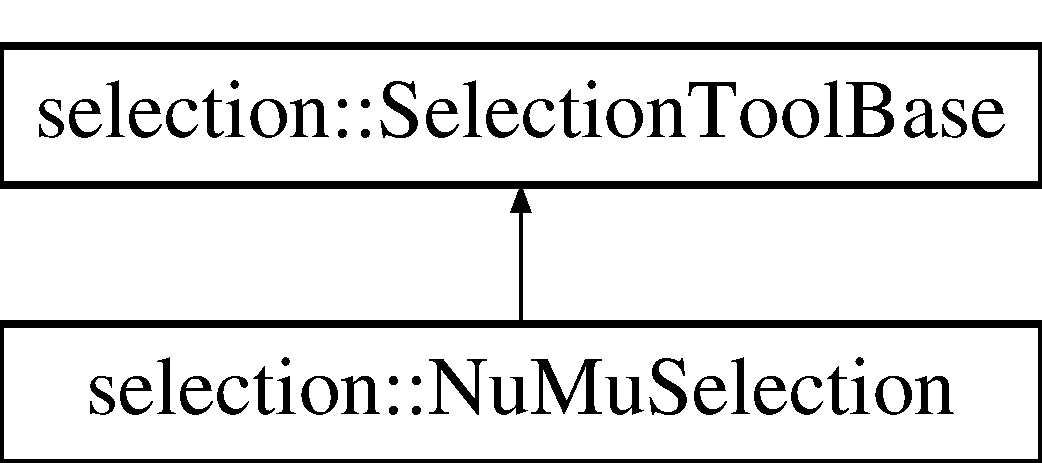
\includegraphics[height=2.000000cm]{classselection_1_1NuMuSelection}
\end{center}
\end{figure}
\subsection*{Public Member Functions}
\begin{DoxyCompactItemize}
\item 
\hyperlink{classselection_1_1NuMuSelection_a6c36dee1cdd9d72715fd43325dfdd585}{Nu\-Mu\-Selection} (const fhicl\-::\-Parameter\-Set \&pset)
\begin{DoxyCompactList}\small\item\em Constructor. \end{DoxyCompactList}\item 
\hypertarget{classselection_1_1NuMuSelection_af2a4b263e268fc51f0fa58ea4ad74ee4}{\hyperlink{classselection_1_1NuMuSelection_af2a4b263e268fc51f0fa58ea4ad74ee4}{$\sim$\-Nu\-Mu\-Selection} ()}\label{classselection_1_1NuMuSelection_af2a4b263e268fc51f0fa58ea4ad74ee4}

\begin{DoxyCompactList}\small\item\em Destructor. \end{DoxyCompactList}\item 
void \hyperlink{classselection_1_1NuMuSelection_a81a56e38f0c105c5ef34a3c777c2ff1d}{configure} (fhicl\-::\-Parameter\-Set const \&pset)
\item 
bool \hyperlink{classselection_1_1NuMuSelection_ad9aaf5eedf311e33cb6e7f54e2605c98}{select\-Event} (art\-::\-Event const \&e, const std\-::vector$<$ Proxy\-Pfp\-Elem\-\_\-t $>$ \&pfp\-\_\-pxy\-\_\-v)
\begin{DoxyCompactList}\small\item\em Selection function. \end{DoxyCompactList}\item 
void \hyperlink{classselection_1_1NuMuSelection_ac8305341911433f5e08ee705280199d4}{set\-Branches} (T\-Tree $\ast$\-\_\-tree)
\begin{DoxyCompactList}\small\item\em Set branches for T\-Tree. \end{DoxyCompactList}\item 
void \hyperlink{classselection_1_1NuMuSelection_a18b4df2675c0622cb5fbe00711350328}{reset\-T\-Tree} (T\-Tree $\ast$\-\_\-tree)
\begin{DoxyCompactList}\small\item\em Reset T\-Tree branches. \end{DoxyCompactList}\item 
bool \hyperlink{classselection_1_1NuMuSelection_a8d363b7e57166d4711020245db1b73b1}{is\-Fiducial} (const double x\mbox{[}3\mbox{]}) const 
\begin{DoxyCompactList}\small\item\em Check if point is inside fiducial volume. \end{DoxyCompactList}\end{DoxyCompactItemize}
\subsection*{Private Attributes}
\begin{DoxyCompactItemize}
\item 
\hypertarget{classselection_1_1NuMuSelection_a185927f3dc298ec0b8296be2c8648141}{trkf\-::\-Track\-Momentum\-Calculator {\bfseries \-\_\-trkmom}}\label{classselection_1_1NuMuSelection_a185927f3dc298ec0b8296be2c8648141}

\item 
\hypertarget{classselection_1_1NuMuSelection_ab8e07cbd8525b836dab50d64763601f9}{T\-Particle\-P\-D\-G $\ast$ {\bfseries proton} = T\-Database\-P\-D\-G\-::\-Instance()-\/$>$Get\-Particle(2212)}\label{classselection_1_1NuMuSelection_ab8e07cbd8525b836dab50d64763601f9}

\item 
\hypertarget{classselection_1_1NuMuSelection_a5ba2d705b86b01d5dc3e81bef4c7f529}{T\-Particle\-P\-D\-G $\ast$ {\bfseries electron} = T\-Database\-P\-D\-G\-::\-Instance()-\/$>$Get\-Particle(11)}\label{classselection_1_1NuMuSelection_a5ba2d705b86b01d5dc3e81bef4c7f529}

\item 
\hypertarget{classselection_1_1NuMuSelection_a3febed51a71a8cdb52ef098c7ceaccf3}{T\-Particle\-P\-D\-G $\ast$ {\bfseries muon} = T\-Database\-P\-D\-G\-::\-Instance()-\/$>$Get\-Particle(13)}\label{classselection_1_1NuMuSelection_a3febed51a71a8cdb52ef098c7ceaccf3}

\item 
\hypertarget{classselection_1_1NuMuSelection_ad69c6385b7bdb99a3a85bc9d48555ca7}{T\-Particle\-P\-D\-G $\ast$ {\bfseries pion} = T\-Database\-P\-D\-G\-::\-Instance()-\/$>$Get\-Particle(211)}\label{classselection_1_1NuMuSelection_ad69c6385b7bdb99a3a85bc9d48555ca7}

\item 
\hypertarget{classselection_1_1NuMuSelection_ab5f0dc22ab81c743cbb880c048901f75}{T\-Particle\-P\-D\-G $\ast$ {\bfseries kaon} = T\-Database\-P\-D\-G\-::\-Instance()-\/$>$Get\-Particle(321)}\label{classselection_1_1NuMuSelection_ab5f0dc22ab81c743cbb880c048901f75}

\item 
float \hyperlink{classselection_1_1NuMuSelection_ad112dbbc5a443a1ff5408c512788a154}{f\-Trk\-Shrscore}
\item 
float \hyperlink{classselection_1_1NuMuSelection_afd0602fc9b69392ffb8dbc36c6ff3e61}{f\-Fidvol\-Zstart}
\item 
float \hyperlink{classselection_1_1NuMuSelection_adae665ca6cf1ece4b7e00b345cebbfe3}{f\-Fidvol\-Zend}
\item 
float \hyperlink{classselection_1_1NuMuSelection_a68277003f5211d751a5965dc990ff661}{f\-Fidvol\-Ystart}
\item 
float \hyperlink{classselection_1_1NuMuSelection_ac07847d191d7d4db8267d89e0caab414}{f\-Fidvol\-Yend}
\item 
float \hyperlink{classselection_1_1NuMuSelection_a5f015a245b7a149756f787f2dab9fcc7}{f\-Fidvol\-Xstart}
\item 
float \hyperlink{classselection_1_1NuMuSelection_ab57daae1ee3ed13b58016eb68f0d6712}{f\-Fidvol\-Xend}
\item 
\hypertarget{classselection_1_1NuMuSelection_a2b42e74d57763e5b49f6fd1123bdb154}{art\-::\-Input\-Tag {\bfseries f\-C\-L\-Sproducer}}\label{classselection_1_1NuMuSelection_a2b42e74d57763e5b49f6fd1123bdb154}

\item 
\hypertarget{classselection_1_1NuMuSelection_a54685a2abfa66dbf5a08cc58e215c013}{art\-::\-Input\-Tag {\bfseries f\-P\-I\-Dproducer}}\label{classselection_1_1NuMuSelection_a54685a2abfa66dbf5a08cc58e215c013}

\item 
\hypertarget{classselection_1_1NuMuSelection_aa458d765d2088552375177afa2006b08}{art\-::\-Input\-Tag {\bfseries f\-T\-R\-Kproducer}}\label{classselection_1_1NuMuSelection_aa458d765d2088552375177afa2006b08}

\item 
\hypertarget{classselection_1_1NuMuSelection_af12bf233739d67542d69294088a68336}{art\-::\-Input\-Tag {\bfseries f\-T\-R\-Kproducer\-Trk\-Fit}}\label{classselection_1_1NuMuSelection_af12bf233739d67542d69294088a68336}

\item 
\hypertarget{classselection_1_1NuMuSelection_a05394c48def95fa5e6334d48e278fe07}{art\-::\-Input\-Tag {\bfseries f\-Backtrack\-Tag}}\label{classselection_1_1NuMuSelection_a05394c48def95fa5e6334d48e278fe07}

\item 
\hypertarget{classselection_1_1NuMuSelection_a727573fc11e39692e79d8436b04c3ba9}{art\-::\-Input\-Tag {\bfseries f\-Hproducer}}\label{classselection_1_1NuMuSelection_a727573fc11e39692e79d8436b04c3ba9}

\item 
\hypertarget{classselection_1_1NuMuSelection_a76ab636afef2099825cc9e91ca5137e1}{art\-::\-Input\-Tag {\bfseries f\-M\-C\-Rproducer}}\label{classselection_1_1NuMuSelection_a76ab636afef2099825cc9e91ca5137e1}

\item 
\hypertarget{classselection_1_1NuMuSelection_a44a5a71367f35560a9a8783615945c6a}{art\-::\-Input\-Tag {\bfseries f\-M\-C\-Pproducer}}\label{classselection_1_1NuMuSelection_a44a5a71367f35560a9a8783615945c6a}

\item 
\hypertarget{classselection_1_1NuMuSelection_a701a4c68c0a99ccbc07ddcc71fcb5537}{art\-::\-Input\-Tag {\bfseries f\-C\-A\-Lproducer}}\label{classselection_1_1NuMuSelection_a701a4c68c0a99ccbc07ddcc71fcb5537}

\item 
\hypertarget{classselection_1_1NuMuSelection_ad11b6ebb0af319639fc473c46c384ff9}{art\-::\-Input\-Tag {\bfseries f\-C\-A\-Lproducer\-Trk\-Fit}}\label{classselection_1_1NuMuSelection_ad11b6ebb0af319639fc473c46c384ff9}

\item 
unsigned int \hyperlink{classselection_1_1NuMuSelection_a8583770de84e76b78e7ddfb4b7e733da}{\-\_\-n\-\_\-showers\-\_\-contained}
\item 
unsigned int \hyperlink{classselection_1_1NuMuSelection_a4f7501393a59de50a8547b6ff2f286b8}{\-\_\-n\-\_\-tracks\-\_\-contained}
\item 
unsigned int \hyperlink{classselection_1_1NuMuSelection_ab314b2264e547d258e88d2f773352b9f}{\-\_\-shr\-\_\-hits\-\_\-max}
\item 
unsigned int \hyperlink{classselection_1_1NuMuSelection_a3e0166490638c0d08a3b66de9ed1ec91}{\-\_\-trk\-\_\-hits\-\_\-max}
\item 
unsigned int \hyperlink{classselection_1_1NuMuSelection_a9233cd2b1aa05f66da7c04f99ff99058}{\-\_\-shr\-\_\-hits\-\_\-tot}
\item 
unsigned int \hyperlink{classselection_1_1NuMuSelection_abcc3673c89468d4af37e7936ac5716ea}{\-\_\-trk\-\_\-hits\-\_\-tot}
\item 
unsigned int \hyperlink{classselection_1_1NuMuSelection_a7c0ae4ea16390adf8803846578ad2d05}{\-\_\-trk\-\_\-hits\-\_\-y\-\_\-tot}
\item 
unsigned int \hyperlink{classselection_1_1NuMuSelection_adf551288be333a585b4fe8b111b8d3dc}{\-\_\-trk\-\_\-hits\-\_\-v\-\_\-tot}
\item 
unsigned int \hyperlink{classselection_1_1NuMuSelection_ab9a14b2e6823b5309c44d17e343087c6}{\-\_\-trk\-\_\-hits\-\_\-u\-\_\-tot}
\item 
unsigned int \hyperlink{classselection_1_1NuMuSelection_a2d08099d9037a3bc8b3b5c7de3de4b4f}{\-\_\-shr\-\_\-hits\-\_\-y\-\_\-tot}
\item 
unsigned int \hyperlink{classselection_1_1NuMuSelection_aa2d62d528b55bfbb0964fa68f2d0ff04}{\-\_\-shr\-\_\-hits\-\_\-v\-\_\-tot}
\item 
unsigned int \hyperlink{classselection_1_1NuMuSelection_aa88c0578a68ec301fecbe3262aa44762}{\-\_\-shr\-\_\-hits\-\_\-u\-\_\-tot}
\item 
float \hyperlink{classselection_1_1NuMuSelection_a06ebfacd01494668815b794a793e58cf}{\-\_\-shr\-\_\-energy}
\item 
float \hyperlink{classselection_1_1NuMuSelection_a73da6cca89a0a1a854297f4d0a2ac851}{\-\_\-shr\-\_\-energy\-\_\-tot}
\item 
float \hyperlink{classselection_1_1NuMuSelection_a94dda0e5c78c02e5787f00ded787f7ab}{\-\_\-shr\-\_\-dedx\-\_\-\-Y}
\item 
float \hyperlink{classselection_1_1NuMuSelection_a779a5d2a981609620e58ecb9cc476757}{\-\_\-shr\-\_\-dedx\-\_\-\-V}
\item 
float \hyperlink{classselection_1_1NuMuSelection_a208bf1de9d20aa592d340dd331d6a524}{\-\_\-shr\-\_\-dedx\-\_\-\-U}
\item 
float \hyperlink{classselection_1_1NuMuSelection_a2da7e7448ef5334cb3988e5d7be786f3}{\-\_\-shr\-\_\-distance}
\item 
float \hyperlink{classselection_1_1NuMuSelection_a046903808fefc33bee41d19b1f6a96de}{\-\_\-tksh\-\_\-distance}
\item 
float \hyperlink{classselection_1_1NuMuSelection_a129f335453ed7ff4678f2e388ce17575}{\-\_\-tksh\-\_\-angle}
\item 
float \hyperlink{classselection_1_1NuMuSelection_a3aefddb8bd817a3ddd32076f1cf7b291}{\-\_\-shr\-\_\-score}
\item 
float \hyperlink{classselection_1_1NuMuSelection_a721b8729afb4676418e64ae74dfc24fe}{\-\_\-shr\-\_\-theta}
\item 
float \hyperlink{classselection_1_1NuMuSelection_a232af76713ec76fb68ce4e878cc3cbea}{\-\_\-shr\-\_\-phi}
\item 
float \hyperlink{classselection_1_1NuMuSelection_a847713ed8d6765bae1c2f6f590af875d}{\-\_\-shr\-\_\-px}
\item 
float \hyperlink{classselection_1_1NuMuSelection_ac3c72fc9664d3d214a2775a5aa812fbf}{\-\_\-shr\-\_\-py}
\item 
float \hyperlink{classselection_1_1NuMuSelection_ad9b6318a95801512e9ce04c3f61e11f9}{\-\_\-shr\-\_\-pz}
\item 
float \hyperlink{classselection_1_1NuMuSelection_a60e7ec002826c7bc6f31739a1f06d67a}{\-\_\-shr\-\_\-pca\-\_\-0}
\item 
float \hyperlink{classselection_1_1NuMuSelection_a7b9ce353bdf801c126b949d2ababcdef}{\-\_\-shr\-\_\-pca\-\_\-1}
\item 
float \hyperlink{classselection_1_1NuMuSelection_af4069f6356b76cbfb2b2657e70961b63}{\-\_\-shr\-\_\-pca\-\_\-2}
\item 
float \hyperlink{classselection_1_1NuMuSelection_ae0b0231c9373f62ab299817893c3d5f4}{\-\_\-shr\-\_\-openangle}
\item 
float \hyperlink{classselection_1_1NuMuSelection_aaf417a519bc8ecc0d965ac58aff47417}{\-\_\-shr\-\_\-pidchipr}
\item 
float \hyperlink{classselection_1_1NuMuSelection_aba9f56f7c16447322e3108dc91bc3ff0}{\-\_\-shr\-\_\-pidchimu}
\item 
float \hyperlink{classselection_1_1NuMuSelection_af7b55d564aef645da1ff8a1fa0b4e620}{\-\_\-shr\-\_\-bragg\-\_\-p}
\item 
float \hyperlink{classselection_1_1NuMuSelection_aea36ed7e354b16fc1e5ff97cedb23c47}{\-\_\-shr\-\_\-bragg\-\_\-mu}
\item 
float \hyperlink{classselection_1_1NuMuSelection_a418742070b70e6cd789a9dce1572c918}{\-\_\-shr\-\_\-bragg\-\_\-mip}
\item 
float \hyperlink{classselection_1_1NuMuSelection_a965ff03e4cd45fa4a7267f2c4576c99e}{\-\_\-shr\-\_\-bragg\-\_\-pion}
\item 
float \hyperlink{classselection_1_1NuMuSelection_a32142048875e97db40e44f0b4a51eae3}{\-\_\-shr\-\_\-bragg\-\_\-kaon}
\item 
size\-\_\-t \hyperlink{classselection_1_1NuMuSelection_a6a877911df0beda5d7d43149d0535389}{\-\_\-shr\-\_\-pfp\-\_\-id}
\item 
float \hyperlink{classselection_1_1NuMuSelection_ab8df38bd822646f56b672b4f942930a3}{\-\_\-trk\-\_\-len}
\item 
float \hyperlink{classselection_1_1NuMuSelection_a505f81bb9d920d0304d988a2f3fadbc2}{\-\_\-trk\-\_\-energy}
\item 
float \hyperlink{classselection_1_1NuMuSelection_a62638e6a70986b1b5ae81a3cd80e4dc3}{\-\_\-trk\-\_\-energy\-\_\-tot}
\item 
float \hyperlink{classselection_1_1NuMuSelection_a4d2e1ceec2811a4493f964212b744e26}{\-\_\-trk\-\_\-distance}
\item 
float \hyperlink{classselection_1_1NuMuSelection_a2041fd7980c1dbe98ce5a4c77a305167}{\-\_\-trk\-\_\-theta}
\item 
float \hyperlink{classselection_1_1NuMuSelection_aeb0b180b3bbe753b576c4db2fa3f94af}{\-\_\-trk\-\_\-phi}
\item 
size\-\_\-t \hyperlink{classselection_1_1NuMuSelection_acbc163e95eec5a3bbbf3648480737a56}{\-\_\-trk\-\_\-pfp\-\_\-id}
\item 
float \hyperlink{classselection_1_1NuMuSelection_a550c6e1bb4c959af5f5724b122b39999}{\-\_\-hits\-\_\-ratio}
\item 
float \hyperlink{classselection_1_1NuMuSelection_a14e0373dc5bdb3b21399f45b7313294c}{\-\_\-trk\-\_\-bragg\-\_\-p}
\item 
float \hyperlink{classselection_1_1NuMuSelection_a51cf3e575038967284eb7ff10eeba9e0}{\-\_\-trk\-\_\-bragg\-\_\-mu}
\item 
float \hyperlink{classselection_1_1NuMuSelection_acf6657ef58eba53a46c0a8c9057ff170}{\-\_\-trk\-\_\-bragg\-\_\-mip}
\item 
float \hyperlink{classselection_1_1NuMuSelection_ae68f8cd5aba5ad848ac6ef0576ce6039}{\-\_\-trk\-\_\-bragg\-\_\-pion}
\item 
float \hyperlink{classselection_1_1NuMuSelection_a8fb54244ae254a42f6238bca2d7fb34e}{\-\_\-trk\-\_\-bragg\-\_\-kaon}
\item 
float \hyperlink{classselection_1_1NuMuSelection_af65eea94c4d2811de82693751684131d}{\-\_\-trk\-\_\-pidchipr}
\item 
float \hyperlink{classselection_1_1NuMuSelection_ad0b2f58434040e2c9e9304a93252d5e1}{\-\_\-trk\-\_\-pidchipr\-\_\-best}
\item 
float \hyperlink{classselection_1_1NuMuSelection_a0373f32c36b713af9febf4e5e3b6899a}{\-\_\-trk\-\_\-pidchipr\-\_\-worst}
\item 
float \hyperlink{classselection_1_1NuMuSelection_a3ae2c291adeedd490d43b915257553f7}{\-\_\-trk\-\_\-pidchimu}
\item 
float \hyperlink{classselection_1_1NuMuSelection_ae2b400954b0bce9930437be4fdb7fd85}{\-\_\-trk\-\_\-pida}
\item 
float \hyperlink{classselection_1_1NuMuSelection_a2316596a59c6b87ea5aa75716c588117}{\-\_\-trk\-\_\-score}
\item 
float \hyperlink{classselection_1_1NuMuSelection_aab5bb47332ae2489a5ab96078397d075}{\-\_\-pt}
\item 
float \hyperlink{classselection_1_1NuMuSelection_a821979901c138eca118246a1eeedcd80}{\-\_\-p}
\item 
float \hyperlink{classselection_1_1NuMuSelection_a6988cb9e869c0205f44659b3a65bd047}{\-\_\-shr\-\_\-bkt\-\_\-purity}
\item 
float \hyperlink{classselection_1_1NuMuSelection_a18224668e51654b8322757c2db5d8b9d}{\-\_\-shr\-\_\-bkt\-\_\-completeness}
\item 
float \hyperlink{classselection_1_1NuMuSelection_aa6e475979c9554cb14bf7a082385a128}{\-\_\-shr\-\_\-bkt\-\_\-\-E}
\item 
int \hyperlink{classselection_1_1NuMuSelection_ab5695d0d13afa6fe27e38b63951ade58}{\-\_\-shr\-\_\-bkt\-\_\-pdg}
\item 
float \hyperlink{classselection_1_1NuMuSelection_a72c22e0de99d58873fa4e9824e094c50}{\-\_\-trk\-\_\-bkt\-\_\-purity}
\item 
float \hyperlink{classselection_1_1NuMuSelection_a569e5b1199f57a2becbd28ee0202baae}{\-\_\-trk\-\_\-bkt\-\_\-completeness}
\item 
float \hyperlink{classselection_1_1NuMuSelection_a1957763f4a43de544b42a9e04cf83afa}{\-\_\-trk\-\_\-bkt\-\_\-\-E}
\item 
int \hyperlink{classselection_1_1NuMuSelection_afc6475990e683ff735846740580cac9b}{\-\_\-trk\-\_\-bkt\-\_\-pdg}
\item 
float \hyperlink{classselection_1_1NuMuSelection_a47c185ab6ea19a597c0d049359e851e1}{\-\_\-matched\-\_\-\-E}
\item 
float \hyperlink{classselection_1_1NuMuSelection_a2e7f6e41acd96cb4ff217b1ec129884e}{\-\_\-shr\-\_\-tkfit\-\_\-start\-\_\-x}
\item 
float \hyperlink{classselection_1_1NuMuSelection_aced5ceef2d92e448cfed37ec3fb75ab4}{\-\_\-shr\-\_\-tkfit\-\_\-start\-\_\-y}
\item 
float \hyperlink{classselection_1_1NuMuSelection_a82f756e0a512e9b2ab45a0d2061d2ec3}{\-\_\-shr\-\_\-tkfit\-\_\-start\-\_\-z}
\item 
float \hyperlink{classselection_1_1NuMuSelection_af38dabc2591bc0a81c564db0bb773d2c}{\-\_\-shr\-\_\-start\-\_\-x}
\item 
float \hyperlink{classselection_1_1NuMuSelection_af6c46477cac6efcb513d028e39f707d2}{\-\_\-shr\-\_\-start\-\_\-y}
\item 
float \hyperlink{classselection_1_1NuMuSelection_a9ecc838bf83d8279c7e975aff432f06e}{\-\_\-shr\-\_\-start\-\_\-z}
\item 
float \hyperlink{classselection_1_1NuMuSelection_a82badfd521973f96eb8e2b04d2d768f1}{\-\_\-shr\-\_\-tkfit\-\_\-phi}
\item 
float \hyperlink{classselection_1_1NuMuSelection_a8a3b5a7f7bc6fa4a59fbc36bfbf5a835}{\-\_\-shr\-\_\-tkfit\-\_\-theta}
\item 
float \hyperlink{classselection_1_1NuMuSelection_a1a04003daefae9bb8088709dae0705ca}{\-\_\-shr\-\_\-tkfit\-\_\-dedx\-\_\-\-Y}
\item 
float \hyperlink{classselection_1_1NuMuSelection_a9a054c559dfa6e536562f2e74d2954e0}{\-\_\-shr\-\_\-tkfit\-\_\-dedx\-\_\-\-V}
\item 
float \hyperlink{classselection_1_1NuMuSelection_ab7a3a2abb7bf04a5e3d6a190d1c8c415}{\-\_\-shr\-\_\-tkfit\-\_\-dedx\-\_\-\-U}
\item 
unsigned int \hyperlink{classselection_1_1NuMuSelection_a8104bfe11a01a3afc80e48eebf0b4f1f}{\-\_\-shr\-\_\-tkfit\-\_\-nhits\-\_\-\-Y}
\item 
unsigned int \hyperlink{classselection_1_1NuMuSelection_a089d245ba837cfc077d5f30dd1a309b5}{\-\_\-shr\-\_\-tkfit\-\_\-nhits\-\_\-\-V}
\item 
unsigned int \hyperlink{classselection_1_1NuMuSelection_a49ecf4415ef54632faa2317814210b36}{\-\_\-shr\-\_\-tkfit\-\_\-nhits\-\_\-\-U}
\item 
unsigned int \hyperlink{classselection_1_1NuMuSelection_ac2073c16d1ba83437d9fa66b0aa3ea38}{\-\_\-hits\-\_\-outfv}
\item 
float \hyperlink{classselection_1_1NuMuSelection_a5d7cbf03836116170b56615ab3b073c2}{\-\_\-contained\-\_\-fraction}
\item 
float \hyperlink{classselection_1_1NuMuSelection_a62b2fc85963f5b8c09b9a6306afbb84a}{\-\_\-trk\-\_\-energy\-\_\-hits\-\_\-tot}
\item 
unsigned int \hyperlink{classselection_1_1NuMuSelection_a6c1ae5a457aa2734684c6632abf34a8c}{\-\_\-total\-\_\-hits\-\_\-y}
\item 
float \hyperlink{classselection_1_1NuMuSelection_a9bbe9a46450cfb58e3559d943a5822c8}{\-\_\-extra\-\_\-energy\-\_\-y}
\end{DoxyCompactItemize}
\subsection*{Additional Inherited Members}


\subsection{Detailed Description}
Selection of electron neutrinos with 0 pions and at least on proton in the final state Author\-: Stefano Roberto Soleti (\href{mailto:srsoleti@fnal.gov}{\tt srsoleti@fnal.\-gov}) 

\subsection{Constructor \& Destructor Documentation}
\hypertarget{classselection_1_1NuMuSelection_a6c36dee1cdd9d72715fd43325dfdd585}{\index{selection\-::\-Nu\-Mu\-Selection@{selection\-::\-Nu\-Mu\-Selection}!Nu\-Mu\-Selection@{Nu\-Mu\-Selection}}
\index{Nu\-Mu\-Selection@{Nu\-Mu\-Selection}!selection::NuMuSelection@{selection\-::\-Nu\-Mu\-Selection}}
\subsubsection[{Nu\-Mu\-Selection}]{\setlength{\rightskip}{0pt plus 5cm}selection\-::\-Nu\-Mu\-Selection\-::\-Nu\-Mu\-Selection (
\begin{DoxyParamCaption}
\item[{const fhicl\-::\-Parameter\-Set \&}]{pset}
\end{DoxyParamCaption}
)}}\label{classselection_1_1NuMuSelection_a6c36dee1cdd9d72715fd43325dfdd585}


Constructor. 


\begin{DoxyParams}{Parameters}
{\em pset} & List of parameters in the F\-C\-L file\\
\hline
\end{DoxyParams}
Constructor.

Arguments\-:

pset -\/ Fcl parameters. 

\subsection{Member Function Documentation}
\hypertarget{classselection_1_1NuMuSelection_a81a56e38f0c105c5ef34a3c777c2ff1d}{\index{selection\-::\-Nu\-Mu\-Selection@{selection\-::\-Nu\-Mu\-Selection}!configure@{configure}}
\index{configure@{configure}!selection::NuMuSelection@{selection\-::\-Nu\-Mu\-Selection}}
\subsubsection[{configure}]{\setlength{\rightskip}{0pt plus 5cm}void selection\-::\-Nu\-Mu\-Selection\-::configure (
\begin{DoxyParamCaption}
\item[{fhicl\-::\-Parameter\-Set const \&}]{pset}
\end{DoxyParamCaption}
)}}\label{classselection_1_1NuMuSelection_a81a56e38f0c105c5ef34a3c777c2ff1d}
Reconfigure method.

Arguments\-:

pset -\/ Fcl parameter set. \hypertarget{classselection_1_1NuMuSelection_a8d363b7e57166d4711020245db1b73b1}{\index{selection\-::\-Nu\-Mu\-Selection@{selection\-::\-Nu\-Mu\-Selection}!is\-Fiducial@{is\-Fiducial}}
\index{is\-Fiducial@{is\-Fiducial}!selection::NuMuSelection@{selection\-::\-Nu\-Mu\-Selection}}
\subsubsection[{is\-Fiducial}]{\setlength{\rightskip}{0pt plus 5cm}bool selection\-::\-Nu\-Mu\-Selection\-::is\-Fiducial (
\begin{DoxyParamCaption}
\item[{const double}]{x\mbox{[}3\mbox{]}}
\end{DoxyParamCaption}
) const}}\label{classselection_1_1NuMuSelection_a8d363b7e57166d4711020245db1b73b1}


Check if point is inside fiducial volume. 


\begin{DoxyParams}{Parameters}
{\em x} & array of coordinates \\
\hline
\end{DoxyParams}
\hypertarget{classselection_1_1NuMuSelection_a18b4df2675c0622cb5fbe00711350328}{\index{selection\-::\-Nu\-Mu\-Selection@{selection\-::\-Nu\-Mu\-Selection}!reset\-T\-Tree@{reset\-T\-Tree}}
\index{reset\-T\-Tree@{reset\-T\-Tree}!selection::NuMuSelection@{selection\-::\-Nu\-Mu\-Selection}}
\subsubsection[{reset\-T\-Tree}]{\setlength{\rightskip}{0pt plus 5cm}void selection\-::\-Nu\-Mu\-Selection\-::reset\-T\-Tree (
\begin{DoxyParamCaption}
\item[{T\-Tree $\ast$}]{\-\_\-tree}
\end{DoxyParamCaption}
)\hspace{0.3cm}{\ttfamily [virtual]}}}\label{classselection_1_1NuMuSelection_a18b4df2675c0622cb5fbe00711350328}


Reset T\-Tree branches. 


\begin{DoxyParams}{Parameters}
{\em \-\_\-tree} & R\-O\-O\-T T\-Tree with the selection information \\
\hline
\end{DoxyParams}


Implements \hyperlink{classselection_1_1SelectionToolBase_ae51d9c23ceee13bebf196d6535d5f1a5}{selection\-::\-Selection\-Tool\-Base}.

\hypertarget{classselection_1_1NuMuSelection_ad9aaf5eedf311e33cb6e7f54e2605c98}{\index{selection\-::\-Nu\-Mu\-Selection@{selection\-::\-Nu\-Mu\-Selection}!select\-Event@{select\-Event}}
\index{select\-Event@{select\-Event}!selection::NuMuSelection@{selection\-::\-Nu\-Mu\-Selection}}
\subsubsection[{select\-Event}]{\setlength{\rightskip}{0pt plus 5cm}bool selection\-::\-Nu\-Mu\-Selection\-::select\-Event (
\begin{DoxyParamCaption}
\item[{art\-::\-Event const \&}]{e, }
\item[{const std\-::vector$<$ Proxy\-Pfp\-Elem\-\_\-t $>$ \&}]{pfp\-\_\-pxy\-\_\-v}
\end{DoxyParamCaption}
)\hspace{0.3cm}{\ttfamily [virtual]}}}\label{classselection_1_1NuMuSelection_ad9aaf5eedf311e33cb6e7f54e2605c98}


Selection function. 


\begin{DoxyParams}{Parameters}
{\em e} & art Event \\
\hline
{\em pfp\-\_\-pxy\-\_\-v} & Proxy of P\-F\-Particle vector in the slice\\
\hline
\end{DoxyParams}
Reconfigure method.

Arguments\-:

pset -\/ Fcl parameter set. 

Implements \hyperlink{classselection_1_1SelectionToolBase_ab63818dac49b43418fe9eb3b8cd98c9c}{selection\-::\-Selection\-Tool\-Base}.

\hypertarget{classselection_1_1NuMuSelection_ac8305341911433f5e08ee705280199d4}{\index{selection\-::\-Nu\-Mu\-Selection@{selection\-::\-Nu\-Mu\-Selection}!set\-Branches@{set\-Branches}}
\index{set\-Branches@{set\-Branches}!selection::NuMuSelection@{selection\-::\-Nu\-Mu\-Selection}}
\subsubsection[{set\-Branches}]{\setlength{\rightskip}{0pt plus 5cm}void selection\-::\-Nu\-Mu\-Selection\-::set\-Branches (
\begin{DoxyParamCaption}
\item[{T\-Tree $\ast$}]{\-\_\-tree}
\end{DoxyParamCaption}
)\hspace{0.3cm}{\ttfamily [virtual]}}}\label{classselection_1_1NuMuSelection_ac8305341911433f5e08ee705280199d4}


Set branches for T\-Tree. 


\begin{DoxyParams}{Parameters}
{\em \-\_\-tree} & R\-O\-O\-T T\-Tree with the selection information \\
\hline
\end{DoxyParams}


Implements \hyperlink{classselection_1_1SelectionToolBase_aa97ea5e55391240d8e251dae13897996}{selection\-::\-Selection\-Tool\-Base}.



\subsection{Member Data Documentation}
\hypertarget{classselection_1_1NuMuSelection_a5d7cbf03836116170b56615ab3b073c2}{\index{selection\-::\-Nu\-Mu\-Selection@{selection\-::\-Nu\-Mu\-Selection}!\-\_\-contained\-\_\-fraction@{\-\_\-contained\-\_\-fraction}}
\index{\-\_\-contained\-\_\-fraction@{\-\_\-contained\-\_\-fraction}!selection::NuMuSelection@{selection\-::\-Nu\-Mu\-Selection}}
\subsubsection[{\-\_\-contained\-\_\-fraction}]{\setlength{\rightskip}{0pt plus 5cm}float selection\-::\-Nu\-Mu\-Selection\-::\-\_\-contained\-\_\-fraction\hspace{0.3cm}{\ttfamily [private]}}}\label{classselection_1_1NuMuSelection_a5d7cbf03836116170b56615ab3b073c2}
Fraction of hits of the P\-F\-Particles contained in the fiducial volume \hypertarget{classselection_1_1NuMuSelection_a9bbe9a46450cfb58e3559d943a5822c8}{\index{selection\-::\-Nu\-Mu\-Selection@{selection\-::\-Nu\-Mu\-Selection}!\-\_\-extra\-\_\-energy\-\_\-y@{\-\_\-extra\-\_\-energy\-\_\-y}}
\index{\-\_\-extra\-\_\-energy\-\_\-y@{\-\_\-extra\-\_\-energy\-\_\-y}!selection::NuMuSelection@{selection\-::\-Nu\-Mu\-Selection}}
\subsubsection[{\-\_\-extra\-\_\-energy\-\_\-y}]{\setlength{\rightskip}{0pt plus 5cm}float selection\-::\-Nu\-Mu\-Selection\-::\-\_\-extra\-\_\-energy\-\_\-y\hspace{0.3cm}{\ttfamily [private]}}}\label{classselection_1_1NuMuSelection_a9bbe9a46450cfb58e3559d943a5822c8}
Total energy of the unclustered hits on the Y plane \hypertarget{classselection_1_1NuMuSelection_ac2073c16d1ba83437d9fa66b0aa3ea38}{\index{selection\-::\-Nu\-Mu\-Selection@{selection\-::\-Nu\-Mu\-Selection}!\-\_\-hits\-\_\-outfv@{\-\_\-hits\-\_\-outfv}}
\index{\-\_\-hits\-\_\-outfv@{\-\_\-hits\-\_\-outfv}!selection::NuMuSelection@{selection\-::\-Nu\-Mu\-Selection}}
\subsubsection[{\-\_\-hits\-\_\-outfv}]{\setlength{\rightskip}{0pt plus 5cm}unsigned int selection\-::\-Nu\-Mu\-Selection\-::\-\_\-hits\-\_\-outfv\hspace{0.3cm}{\ttfamily [private]}}}\label{classselection_1_1NuMuSelection_ac2073c16d1ba83437d9fa66b0aa3ea38}
Number of hits of P\-F\-Particles outside the fiducial volume \hypertarget{classselection_1_1NuMuSelection_a550c6e1bb4c959af5f5724b122b39999}{\index{selection\-::\-Nu\-Mu\-Selection@{selection\-::\-Nu\-Mu\-Selection}!\-\_\-hits\-\_\-ratio@{\-\_\-hits\-\_\-ratio}}
\index{\-\_\-hits\-\_\-ratio@{\-\_\-hits\-\_\-ratio}!selection::NuMuSelection@{selection\-::\-Nu\-Mu\-Selection}}
\subsubsection[{\-\_\-hits\-\_\-ratio}]{\setlength{\rightskip}{0pt plus 5cm}float selection\-::\-Nu\-Mu\-Selection\-::\-\_\-hits\-\_\-ratio\hspace{0.3cm}{\ttfamily [private]}}}\label{classselection_1_1NuMuSelection_a550c6e1bb4c959af5f5724b122b39999}
Ratio between hits from showers and total number of hits \hypertarget{classselection_1_1NuMuSelection_a47c185ab6ea19a597c0d049359e851e1}{\index{selection\-::\-Nu\-Mu\-Selection@{selection\-::\-Nu\-Mu\-Selection}!\-\_\-matched\-\_\-\-E@{\-\_\-matched\-\_\-\-E}}
\index{\-\_\-matched\-\_\-\-E@{\-\_\-matched\-\_\-\-E}!selection::NuMuSelection@{selection\-::\-Nu\-Mu\-Selection}}
\subsubsection[{\-\_\-matched\-\_\-\-E}]{\setlength{\rightskip}{0pt plus 5cm}float selection\-::\-Nu\-Mu\-Selection\-::\-\_\-matched\-\_\-\-E\hspace{0.3cm}{\ttfamily [private]}}}\label{classselection_1_1NuMuSelection_a47c185ab6ea19a597c0d049359e851e1}
Total kinetic energy of the M\-C\-Particles matched to P\-F\-Particles \hypertarget{classselection_1_1NuMuSelection_a8583770de84e76b78e7ddfb4b7e733da}{\index{selection\-::\-Nu\-Mu\-Selection@{selection\-::\-Nu\-Mu\-Selection}!\-\_\-n\-\_\-showers\-\_\-contained@{\-\_\-n\-\_\-showers\-\_\-contained}}
\index{\-\_\-n\-\_\-showers\-\_\-contained@{\-\_\-n\-\_\-showers\-\_\-contained}!selection::NuMuSelection@{selection\-::\-Nu\-Mu\-Selection}}
\subsubsection[{\-\_\-n\-\_\-showers\-\_\-contained}]{\setlength{\rightskip}{0pt plus 5cm}unsigned int selection\-::\-Nu\-Mu\-Selection\-::\-\_\-n\-\_\-showers\-\_\-contained\hspace{0.3cm}{\ttfamily [private]}}}\label{classselection_1_1NuMuSelection_a8583770de84e76b78e7ddfb4b7e733da}
Number of showers with a starting point within the fiducial volume \hypertarget{classselection_1_1NuMuSelection_a4f7501393a59de50a8547b6ff2f286b8}{\index{selection\-::\-Nu\-Mu\-Selection@{selection\-::\-Nu\-Mu\-Selection}!\-\_\-n\-\_\-tracks\-\_\-contained@{\-\_\-n\-\_\-tracks\-\_\-contained}}
\index{\-\_\-n\-\_\-tracks\-\_\-contained@{\-\_\-n\-\_\-tracks\-\_\-contained}!selection::NuMuSelection@{selection\-::\-Nu\-Mu\-Selection}}
\subsubsection[{\-\_\-n\-\_\-tracks\-\_\-contained}]{\setlength{\rightskip}{0pt plus 5cm}unsigned int selection\-::\-Nu\-Mu\-Selection\-::\-\_\-n\-\_\-tracks\-\_\-contained\hspace{0.3cm}{\ttfamily [private]}}}\label{classselection_1_1NuMuSelection_a4f7501393a59de50a8547b6ff2f286b8}
Number of tracks fully contained in the fiducial volume \hypertarget{classselection_1_1NuMuSelection_a821979901c138eca118246a1eeedcd80}{\index{selection\-::\-Nu\-Mu\-Selection@{selection\-::\-Nu\-Mu\-Selection}!\-\_\-p@{\-\_\-p}}
\index{\-\_\-p@{\-\_\-p}!selection::NuMuSelection@{selection\-::\-Nu\-Mu\-Selection}}
\subsubsection[{\-\_\-p}]{\setlength{\rightskip}{0pt plus 5cm}float selection\-::\-Nu\-Mu\-Selection\-::\-\_\-p\hspace{0.3cm}{\ttfamily [private]}}}\label{classselection_1_1NuMuSelection_a821979901c138eca118246a1eeedcd80}
Total reconstructed momentum, assuming all the tracks are protons and all the showers are electrons \hypertarget{classselection_1_1NuMuSelection_aab5bb47332ae2489a5ab96078397d075}{\index{selection\-::\-Nu\-Mu\-Selection@{selection\-::\-Nu\-Mu\-Selection}!\-\_\-pt@{\-\_\-pt}}
\index{\-\_\-pt@{\-\_\-pt}!selection::NuMuSelection@{selection\-::\-Nu\-Mu\-Selection}}
\subsubsection[{\-\_\-pt}]{\setlength{\rightskip}{0pt plus 5cm}float selection\-::\-Nu\-Mu\-Selection\-::\-\_\-pt\hspace{0.3cm}{\ttfamily [private]}}}\label{classselection_1_1NuMuSelection_aab5bb47332ae2489a5ab96078397d075}
Total reconstructed transverse momentum, assuming all the tracks are protons and all the showers are electrons \hypertarget{classselection_1_1NuMuSelection_a18224668e51654b8322757c2db5d8b9d}{\index{selection\-::\-Nu\-Mu\-Selection@{selection\-::\-Nu\-Mu\-Selection}!\-\_\-shr\-\_\-bkt\-\_\-completeness@{\-\_\-shr\-\_\-bkt\-\_\-completeness}}
\index{\-\_\-shr\-\_\-bkt\-\_\-completeness@{\-\_\-shr\-\_\-bkt\-\_\-completeness}!selection::NuMuSelection@{selection\-::\-Nu\-Mu\-Selection}}
\subsubsection[{\-\_\-shr\-\_\-bkt\-\_\-completeness}]{\setlength{\rightskip}{0pt plus 5cm}float selection\-::\-Nu\-Mu\-Selection\-::\-\_\-shr\-\_\-bkt\-\_\-completeness\hspace{0.3cm}{\ttfamily [private]}}}\label{classselection_1_1NuMuSelection_a18224668e51654b8322757c2db5d8b9d}
Completeness of the leading shower \hypertarget{classselection_1_1NuMuSelection_aa6e475979c9554cb14bf7a082385a128}{\index{selection\-::\-Nu\-Mu\-Selection@{selection\-::\-Nu\-Mu\-Selection}!\-\_\-shr\-\_\-bkt\-\_\-\-E@{\-\_\-shr\-\_\-bkt\-\_\-\-E}}
\index{\-\_\-shr\-\_\-bkt\-\_\-\-E@{\-\_\-shr\-\_\-bkt\-\_\-\-E}!selection::NuMuSelection@{selection\-::\-Nu\-Mu\-Selection}}
\subsubsection[{\-\_\-shr\-\_\-bkt\-\_\-\-E}]{\setlength{\rightskip}{0pt plus 5cm}float selection\-::\-Nu\-Mu\-Selection\-::\-\_\-shr\-\_\-bkt\-\_\-\-E\hspace{0.3cm}{\ttfamily [private]}}}\label{classselection_1_1NuMuSelection_aa6e475979c9554cb14bf7a082385a128}
Energy of the M\-C\-Particle matched to the leading shower \hypertarget{classselection_1_1NuMuSelection_ab5695d0d13afa6fe27e38b63951ade58}{\index{selection\-::\-Nu\-Mu\-Selection@{selection\-::\-Nu\-Mu\-Selection}!\-\_\-shr\-\_\-bkt\-\_\-pdg@{\-\_\-shr\-\_\-bkt\-\_\-pdg}}
\index{\-\_\-shr\-\_\-bkt\-\_\-pdg@{\-\_\-shr\-\_\-bkt\-\_\-pdg}!selection::NuMuSelection@{selection\-::\-Nu\-Mu\-Selection}}
\subsubsection[{\-\_\-shr\-\_\-bkt\-\_\-pdg}]{\setlength{\rightskip}{0pt plus 5cm}int selection\-::\-Nu\-Mu\-Selection\-::\-\_\-shr\-\_\-bkt\-\_\-pdg\hspace{0.3cm}{\ttfamily [private]}}}\label{classselection_1_1NuMuSelection_ab5695d0d13afa6fe27e38b63951ade58}
P\-D\-G code of the M\-C\-Particle matched to the leading shower \hypertarget{classselection_1_1NuMuSelection_a6988cb9e869c0205f44659b3a65bd047}{\index{selection\-::\-Nu\-Mu\-Selection@{selection\-::\-Nu\-Mu\-Selection}!\-\_\-shr\-\_\-bkt\-\_\-purity@{\-\_\-shr\-\_\-bkt\-\_\-purity}}
\index{\-\_\-shr\-\_\-bkt\-\_\-purity@{\-\_\-shr\-\_\-bkt\-\_\-purity}!selection::NuMuSelection@{selection\-::\-Nu\-Mu\-Selection}}
\subsubsection[{\-\_\-shr\-\_\-bkt\-\_\-purity}]{\setlength{\rightskip}{0pt plus 5cm}float selection\-::\-Nu\-Mu\-Selection\-::\-\_\-shr\-\_\-bkt\-\_\-purity\hspace{0.3cm}{\ttfamily [private]}}}\label{classselection_1_1NuMuSelection_a6988cb9e869c0205f44659b3a65bd047}
Purity of the leading shower \hypertarget{classselection_1_1NuMuSelection_a32142048875e97db40e44f0b4a51eae3}{\index{selection\-::\-Nu\-Mu\-Selection@{selection\-::\-Nu\-Mu\-Selection}!\-\_\-shr\-\_\-bragg\-\_\-kaon@{\-\_\-shr\-\_\-bragg\-\_\-kaon}}
\index{\-\_\-shr\-\_\-bragg\-\_\-kaon@{\-\_\-shr\-\_\-bragg\-\_\-kaon}!selection::NuMuSelection@{selection\-::\-Nu\-Mu\-Selection}}
\subsubsection[{\-\_\-shr\-\_\-bragg\-\_\-kaon}]{\setlength{\rightskip}{0pt plus 5cm}float selection\-::\-Nu\-Mu\-Selection\-::\-\_\-shr\-\_\-bragg\-\_\-kaon\hspace{0.3cm}{\ttfamily [private]}}}\label{classselection_1_1NuMuSelection_a32142048875e97db40e44f0b4a51eae3}
Kaon Bragg likelihood for the leading shower (with the shower reconstructed as track) \hypertarget{classselection_1_1NuMuSelection_a418742070b70e6cd789a9dce1572c918}{\index{selection\-::\-Nu\-Mu\-Selection@{selection\-::\-Nu\-Mu\-Selection}!\-\_\-shr\-\_\-bragg\-\_\-mip@{\-\_\-shr\-\_\-bragg\-\_\-mip}}
\index{\-\_\-shr\-\_\-bragg\-\_\-mip@{\-\_\-shr\-\_\-bragg\-\_\-mip}!selection::NuMuSelection@{selection\-::\-Nu\-Mu\-Selection}}
\subsubsection[{\-\_\-shr\-\_\-bragg\-\_\-mip}]{\setlength{\rightskip}{0pt plus 5cm}float selection\-::\-Nu\-Mu\-Selection\-::\-\_\-shr\-\_\-bragg\-\_\-mip\hspace{0.3cm}{\ttfamily [private]}}}\label{classselection_1_1NuMuSelection_a418742070b70e6cd789a9dce1572c918}
M\-I\-P Bragg likelihood score for the leading shower (with the shower reconstructed as track) \hypertarget{classselection_1_1NuMuSelection_aea36ed7e354b16fc1e5ff97cedb23c47}{\index{selection\-::\-Nu\-Mu\-Selection@{selection\-::\-Nu\-Mu\-Selection}!\-\_\-shr\-\_\-bragg\-\_\-mu@{\-\_\-shr\-\_\-bragg\-\_\-mu}}
\index{\-\_\-shr\-\_\-bragg\-\_\-mu@{\-\_\-shr\-\_\-bragg\-\_\-mu}!selection::NuMuSelection@{selection\-::\-Nu\-Mu\-Selection}}
\subsubsection[{\-\_\-shr\-\_\-bragg\-\_\-mu}]{\setlength{\rightskip}{0pt plus 5cm}float selection\-::\-Nu\-Mu\-Selection\-::\-\_\-shr\-\_\-bragg\-\_\-mu\hspace{0.3cm}{\ttfamily [private]}}}\label{classselection_1_1NuMuSelection_aea36ed7e354b16fc1e5ff97cedb23c47}
Muon Bragg likelihood score for the leading shower (with the shower reconstructed as track) \hypertarget{classselection_1_1NuMuSelection_af7b55d564aef645da1ff8a1fa0b4e620}{\index{selection\-::\-Nu\-Mu\-Selection@{selection\-::\-Nu\-Mu\-Selection}!\-\_\-shr\-\_\-bragg\-\_\-p@{\-\_\-shr\-\_\-bragg\-\_\-p}}
\index{\-\_\-shr\-\_\-bragg\-\_\-p@{\-\_\-shr\-\_\-bragg\-\_\-p}!selection::NuMuSelection@{selection\-::\-Nu\-Mu\-Selection}}
\subsubsection[{\-\_\-shr\-\_\-bragg\-\_\-p}]{\setlength{\rightskip}{0pt plus 5cm}float selection\-::\-Nu\-Mu\-Selection\-::\-\_\-shr\-\_\-bragg\-\_\-p\hspace{0.3cm}{\ttfamily [private]}}}\label{classselection_1_1NuMuSelection_af7b55d564aef645da1ff8a1fa0b4e620}
Proton Bragg likelihood score for the leading shower (with the shower reconstructed as track) \hypertarget{classselection_1_1NuMuSelection_a965ff03e4cd45fa4a7267f2c4576c99e}{\index{selection\-::\-Nu\-Mu\-Selection@{selection\-::\-Nu\-Mu\-Selection}!\-\_\-shr\-\_\-bragg\-\_\-pion@{\-\_\-shr\-\_\-bragg\-\_\-pion}}
\index{\-\_\-shr\-\_\-bragg\-\_\-pion@{\-\_\-shr\-\_\-bragg\-\_\-pion}!selection::NuMuSelection@{selection\-::\-Nu\-Mu\-Selection}}
\subsubsection[{\-\_\-shr\-\_\-bragg\-\_\-pion}]{\setlength{\rightskip}{0pt plus 5cm}float selection\-::\-Nu\-Mu\-Selection\-::\-\_\-shr\-\_\-bragg\-\_\-pion\hspace{0.3cm}{\ttfamily [private]}}}\label{classselection_1_1NuMuSelection_a965ff03e4cd45fa4a7267f2c4576c99e}
Pion Bragg likelihood for the leading shower (with the shower reconstructed as track) \hypertarget{classselection_1_1NuMuSelection_a208bf1de9d20aa592d340dd331d6a524}{\index{selection\-::\-Nu\-Mu\-Selection@{selection\-::\-Nu\-Mu\-Selection}!\-\_\-shr\-\_\-dedx\-\_\-\-U@{\-\_\-shr\-\_\-dedx\-\_\-\-U}}
\index{\-\_\-shr\-\_\-dedx\-\_\-\-U@{\-\_\-shr\-\_\-dedx\-\_\-\-U}!selection::NuMuSelection@{selection\-::\-Nu\-Mu\-Selection}}
\subsubsection[{\-\_\-shr\-\_\-dedx\-\_\-\-U}]{\setlength{\rightskip}{0pt plus 5cm}float selection\-::\-Nu\-Mu\-Selection\-::\-\_\-shr\-\_\-dedx\-\_\-\-U\hspace{0.3cm}{\ttfamily [private]}}}\label{classselection_1_1NuMuSelection_a208bf1de9d20aa592d340dd331d6a524}
d\-E/dx of the leading shower on the U plane with the 1x4 cm box method \hypertarget{classselection_1_1NuMuSelection_a779a5d2a981609620e58ecb9cc476757}{\index{selection\-::\-Nu\-Mu\-Selection@{selection\-::\-Nu\-Mu\-Selection}!\-\_\-shr\-\_\-dedx\-\_\-\-V@{\-\_\-shr\-\_\-dedx\-\_\-\-V}}
\index{\-\_\-shr\-\_\-dedx\-\_\-\-V@{\-\_\-shr\-\_\-dedx\-\_\-\-V}!selection::NuMuSelection@{selection\-::\-Nu\-Mu\-Selection}}
\subsubsection[{\-\_\-shr\-\_\-dedx\-\_\-\-V}]{\setlength{\rightskip}{0pt plus 5cm}float selection\-::\-Nu\-Mu\-Selection\-::\-\_\-shr\-\_\-dedx\-\_\-\-V\hspace{0.3cm}{\ttfamily [private]}}}\label{classselection_1_1NuMuSelection_a779a5d2a981609620e58ecb9cc476757}
d\-E/dx of the leading shower on the V plane with the 1x4 cm box method \hypertarget{classselection_1_1NuMuSelection_a94dda0e5c78c02e5787f00ded787f7ab}{\index{selection\-::\-Nu\-Mu\-Selection@{selection\-::\-Nu\-Mu\-Selection}!\-\_\-shr\-\_\-dedx\-\_\-\-Y@{\-\_\-shr\-\_\-dedx\-\_\-\-Y}}
\index{\-\_\-shr\-\_\-dedx\-\_\-\-Y@{\-\_\-shr\-\_\-dedx\-\_\-\-Y}!selection::NuMuSelection@{selection\-::\-Nu\-Mu\-Selection}}
\subsubsection[{\-\_\-shr\-\_\-dedx\-\_\-\-Y}]{\setlength{\rightskip}{0pt plus 5cm}float selection\-::\-Nu\-Mu\-Selection\-::\-\_\-shr\-\_\-dedx\-\_\-\-Y\hspace{0.3cm}{\ttfamily [private]}}}\label{classselection_1_1NuMuSelection_a94dda0e5c78c02e5787f00ded787f7ab}
d\-E/dx of the leading shower on the Y plane with the 1x4 cm box method \hypertarget{classselection_1_1NuMuSelection_a2da7e7448ef5334cb3988e5d7be786f3}{\index{selection\-::\-Nu\-Mu\-Selection@{selection\-::\-Nu\-Mu\-Selection}!\-\_\-shr\-\_\-distance@{\-\_\-shr\-\_\-distance}}
\index{\-\_\-shr\-\_\-distance@{\-\_\-shr\-\_\-distance}!selection::NuMuSelection@{selection\-::\-Nu\-Mu\-Selection}}
\subsubsection[{\-\_\-shr\-\_\-distance}]{\setlength{\rightskip}{0pt plus 5cm}float selection\-::\-Nu\-Mu\-Selection\-::\-\_\-shr\-\_\-distance\hspace{0.3cm}{\ttfamily [private]}}}\label{classselection_1_1NuMuSelection_a2da7e7448ef5334cb3988e5d7be786f3}
Distance between leading shower vertex and reconstructed neutrino vertex \hypertarget{classselection_1_1NuMuSelection_a06ebfacd01494668815b794a793e58cf}{\index{selection\-::\-Nu\-Mu\-Selection@{selection\-::\-Nu\-Mu\-Selection}!\-\_\-shr\-\_\-energy@{\-\_\-shr\-\_\-energy}}
\index{\-\_\-shr\-\_\-energy@{\-\_\-shr\-\_\-energy}!selection::NuMuSelection@{selection\-::\-Nu\-Mu\-Selection}}
\subsubsection[{\-\_\-shr\-\_\-energy}]{\setlength{\rightskip}{0pt plus 5cm}float selection\-::\-Nu\-Mu\-Selection\-::\-\_\-shr\-\_\-energy\hspace{0.3cm}{\ttfamily [private]}}}\label{classselection_1_1NuMuSelection_a06ebfacd01494668815b794a793e58cf}
Energy of the shower with the largest number of hits (in Ge\-V) \hypertarget{classselection_1_1NuMuSelection_a73da6cca89a0a1a854297f4d0a2ac851}{\index{selection\-::\-Nu\-Mu\-Selection@{selection\-::\-Nu\-Mu\-Selection}!\-\_\-shr\-\_\-energy\-\_\-tot@{\-\_\-shr\-\_\-energy\-\_\-tot}}
\index{\-\_\-shr\-\_\-energy\-\_\-tot@{\-\_\-shr\-\_\-energy\-\_\-tot}!selection::NuMuSelection@{selection\-::\-Nu\-Mu\-Selection}}
\subsubsection[{\-\_\-shr\-\_\-energy\-\_\-tot}]{\setlength{\rightskip}{0pt plus 5cm}float selection\-::\-Nu\-Mu\-Selection\-::\-\_\-shr\-\_\-energy\-\_\-tot\hspace{0.3cm}{\ttfamily [private]}}}\label{classselection_1_1NuMuSelection_a73da6cca89a0a1a854297f4d0a2ac851}
Sum of the energy of the showers (in Ge\-V) \hypertarget{classselection_1_1NuMuSelection_ab314b2264e547d258e88d2f773352b9f}{\index{selection\-::\-Nu\-Mu\-Selection@{selection\-::\-Nu\-Mu\-Selection}!\-\_\-shr\-\_\-hits\-\_\-max@{\-\_\-shr\-\_\-hits\-\_\-max}}
\index{\-\_\-shr\-\_\-hits\-\_\-max@{\-\_\-shr\-\_\-hits\-\_\-max}!selection::NuMuSelection@{selection\-::\-Nu\-Mu\-Selection}}
\subsubsection[{\-\_\-shr\-\_\-hits\-\_\-max}]{\setlength{\rightskip}{0pt plus 5cm}unsigned int selection\-::\-Nu\-Mu\-Selection\-::\-\_\-shr\-\_\-hits\-\_\-max\hspace{0.3cm}{\ttfamily [private]}}}\label{classselection_1_1NuMuSelection_ab314b2264e547d258e88d2f773352b9f}
Number of hits of the leading shower \hypertarget{classselection_1_1NuMuSelection_a9233cd2b1aa05f66da7c04f99ff99058}{\index{selection\-::\-Nu\-Mu\-Selection@{selection\-::\-Nu\-Mu\-Selection}!\-\_\-shr\-\_\-hits\-\_\-tot@{\-\_\-shr\-\_\-hits\-\_\-tot}}
\index{\-\_\-shr\-\_\-hits\-\_\-tot@{\-\_\-shr\-\_\-hits\-\_\-tot}!selection::NuMuSelection@{selection\-::\-Nu\-Mu\-Selection}}
\subsubsection[{\-\_\-shr\-\_\-hits\-\_\-tot}]{\setlength{\rightskip}{0pt plus 5cm}unsigned int selection\-::\-Nu\-Mu\-Selection\-::\-\_\-shr\-\_\-hits\-\_\-tot\hspace{0.3cm}{\ttfamily [private]}}}\label{classselection_1_1NuMuSelection_a9233cd2b1aa05f66da7c04f99ff99058}
Total number of shower hits \hypertarget{classselection_1_1NuMuSelection_aa88c0578a68ec301fecbe3262aa44762}{\index{selection\-::\-Nu\-Mu\-Selection@{selection\-::\-Nu\-Mu\-Selection}!\-\_\-shr\-\_\-hits\-\_\-u\-\_\-tot@{\-\_\-shr\-\_\-hits\-\_\-u\-\_\-tot}}
\index{\-\_\-shr\-\_\-hits\-\_\-u\-\_\-tot@{\-\_\-shr\-\_\-hits\-\_\-u\-\_\-tot}!selection::NuMuSelection@{selection\-::\-Nu\-Mu\-Selection}}
\subsubsection[{\-\_\-shr\-\_\-hits\-\_\-u\-\_\-tot}]{\setlength{\rightskip}{0pt plus 5cm}unsigned int selection\-::\-Nu\-Mu\-Selection\-::\-\_\-shr\-\_\-hits\-\_\-u\-\_\-tot\hspace{0.3cm}{\ttfamily [private]}}}\label{classselection_1_1NuMuSelection_aa88c0578a68ec301fecbe3262aa44762}
Total number of shower hits on the U plane \hypertarget{classselection_1_1NuMuSelection_aa2d62d528b55bfbb0964fa68f2d0ff04}{\index{selection\-::\-Nu\-Mu\-Selection@{selection\-::\-Nu\-Mu\-Selection}!\-\_\-shr\-\_\-hits\-\_\-v\-\_\-tot@{\-\_\-shr\-\_\-hits\-\_\-v\-\_\-tot}}
\index{\-\_\-shr\-\_\-hits\-\_\-v\-\_\-tot@{\-\_\-shr\-\_\-hits\-\_\-v\-\_\-tot}!selection::NuMuSelection@{selection\-::\-Nu\-Mu\-Selection}}
\subsubsection[{\-\_\-shr\-\_\-hits\-\_\-v\-\_\-tot}]{\setlength{\rightskip}{0pt plus 5cm}unsigned int selection\-::\-Nu\-Mu\-Selection\-::\-\_\-shr\-\_\-hits\-\_\-v\-\_\-tot\hspace{0.3cm}{\ttfamily [private]}}}\label{classselection_1_1NuMuSelection_aa2d62d528b55bfbb0964fa68f2d0ff04}
Total number of shower hits on the V plane \hypertarget{classselection_1_1NuMuSelection_a2d08099d9037a3bc8b3b5c7de3de4b4f}{\index{selection\-::\-Nu\-Mu\-Selection@{selection\-::\-Nu\-Mu\-Selection}!\-\_\-shr\-\_\-hits\-\_\-y\-\_\-tot@{\-\_\-shr\-\_\-hits\-\_\-y\-\_\-tot}}
\index{\-\_\-shr\-\_\-hits\-\_\-y\-\_\-tot@{\-\_\-shr\-\_\-hits\-\_\-y\-\_\-tot}!selection::NuMuSelection@{selection\-::\-Nu\-Mu\-Selection}}
\subsubsection[{\-\_\-shr\-\_\-hits\-\_\-y\-\_\-tot}]{\setlength{\rightskip}{0pt plus 5cm}unsigned int selection\-::\-Nu\-Mu\-Selection\-::\-\_\-shr\-\_\-hits\-\_\-y\-\_\-tot\hspace{0.3cm}{\ttfamily [private]}}}\label{classselection_1_1NuMuSelection_a2d08099d9037a3bc8b3b5c7de3de4b4f}
Total number of shower hits on the Y plane \hypertarget{classselection_1_1NuMuSelection_ae0b0231c9373f62ab299817893c3d5f4}{\index{selection\-::\-Nu\-Mu\-Selection@{selection\-::\-Nu\-Mu\-Selection}!\-\_\-shr\-\_\-openangle@{\-\_\-shr\-\_\-openangle}}
\index{\-\_\-shr\-\_\-openangle@{\-\_\-shr\-\_\-openangle}!selection::NuMuSelection@{selection\-::\-Nu\-Mu\-Selection}}
\subsubsection[{\-\_\-shr\-\_\-openangle}]{\setlength{\rightskip}{0pt plus 5cm}float selection\-::\-Nu\-Mu\-Selection\-::\-\_\-shr\-\_\-openangle\hspace{0.3cm}{\ttfamily [private]}}}\label{classselection_1_1NuMuSelection_ae0b0231c9373f62ab299817893c3d5f4}
Opening angle of the shower \hypertarget{classselection_1_1NuMuSelection_a60e7ec002826c7bc6f31739a1f06d67a}{\index{selection\-::\-Nu\-Mu\-Selection@{selection\-::\-Nu\-Mu\-Selection}!\-\_\-shr\-\_\-pca\-\_\-0@{\-\_\-shr\-\_\-pca\-\_\-0}}
\index{\-\_\-shr\-\_\-pca\-\_\-0@{\-\_\-shr\-\_\-pca\-\_\-0}!selection::NuMuSelection@{selection\-::\-Nu\-Mu\-Selection}}
\subsubsection[{\-\_\-shr\-\_\-pca\-\_\-0}]{\setlength{\rightskip}{0pt plus 5cm}float selection\-::\-Nu\-Mu\-Selection\-::\-\_\-shr\-\_\-pca\-\_\-0\hspace{0.3cm}{\ttfamily [private]}}}\label{classselection_1_1NuMuSelection_a60e7ec002826c7bc6f31739a1f06d67a}
First eigenvalue of the P\-C\-Axis of the leading shower \hypertarget{classselection_1_1NuMuSelection_a7b9ce353bdf801c126b949d2ababcdef}{\index{selection\-::\-Nu\-Mu\-Selection@{selection\-::\-Nu\-Mu\-Selection}!\-\_\-shr\-\_\-pca\-\_\-1@{\-\_\-shr\-\_\-pca\-\_\-1}}
\index{\-\_\-shr\-\_\-pca\-\_\-1@{\-\_\-shr\-\_\-pca\-\_\-1}!selection::NuMuSelection@{selection\-::\-Nu\-Mu\-Selection}}
\subsubsection[{\-\_\-shr\-\_\-pca\-\_\-1}]{\setlength{\rightskip}{0pt plus 5cm}float selection\-::\-Nu\-Mu\-Selection\-::\-\_\-shr\-\_\-pca\-\_\-1\hspace{0.3cm}{\ttfamily [private]}}}\label{classselection_1_1NuMuSelection_a7b9ce353bdf801c126b949d2ababcdef}
Second eigenvalue of the P\-C\-Axis of the leading shower \hypertarget{classselection_1_1NuMuSelection_af4069f6356b76cbfb2b2657e70961b63}{\index{selection\-::\-Nu\-Mu\-Selection@{selection\-::\-Nu\-Mu\-Selection}!\-\_\-shr\-\_\-pca\-\_\-2@{\-\_\-shr\-\_\-pca\-\_\-2}}
\index{\-\_\-shr\-\_\-pca\-\_\-2@{\-\_\-shr\-\_\-pca\-\_\-2}!selection::NuMuSelection@{selection\-::\-Nu\-Mu\-Selection}}
\subsubsection[{\-\_\-shr\-\_\-pca\-\_\-2}]{\setlength{\rightskip}{0pt plus 5cm}float selection\-::\-Nu\-Mu\-Selection\-::\-\_\-shr\-\_\-pca\-\_\-2\hspace{0.3cm}{\ttfamily [private]}}}\label{classselection_1_1NuMuSelection_af4069f6356b76cbfb2b2657e70961b63}
Third eigenvalue of the P\-C\-Axis of the leading shower \hypertarget{classselection_1_1NuMuSelection_a6a877911df0beda5d7d43149d0535389}{\index{selection\-::\-Nu\-Mu\-Selection@{selection\-::\-Nu\-Mu\-Selection}!\-\_\-shr\-\_\-pfp\-\_\-id@{\-\_\-shr\-\_\-pfp\-\_\-id}}
\index{\-\_\-shr\-\_\-pfp\-\_\-id@{\-\_\-shr\-\_\-pfp\-\_\-id}!selection::NuMuSelection@{selection\-::\-Nu\-Mu\-Selection}}
\subsubsection[{\-\_\-shr\-\_\-pfp\-\_\-id}]{\setlength{\rightskip}{0pt plus 5cm}size\-\_\-t selection\-::\-Nu\-Mu\-Selection\-::\-\_\-shr\-\_\-pfp\-\_\-id\hspace{0.3cm}{\ttfamily [private]}}}\label{classselection_1_1NuMuSelection_a6a877911df0beda5d7d43149d0535389}
Index of the leading shower in the P\-F\-Particle vector \hypertarget{classselection_1_1NuMuSelection_a232af76713ec76fb68ce4e878cc3cbea}{\index{selection\-::\-Nu\-Mu\-Selection@{selection\-::\-Nu\-Mu\-Selection}!\-\_\-shr\-\_\-phi@{\-\_\-shr\-\_\-phi}}
\index{\-\_\-shr\-\_\-phi@{\-\_\-shr\-\_\-phi}!selection::NuMuSelection@{selection\-::\-Nu\-Mu\-Selection}}
\subsubsection[{\-\_\-shr\-\_\-phi}]{\setlength{\rightskip}{0pt plus 5cm}float selection\-::\-Nu\-Mu\-Selection\-::\-\_\-shr\-\_\-phi\hspace{0.3cm}{\ttfamily [private]}}}\label{classselection_1_1NuMuSelection_a232af76713ec76fb68ce4e878cc3cbea}
Reconstructed phi angle for the leading shower \hypertarget{classselection_1_1NuMuSelection_aba9f56f7c16447322e3108dc91bc3ff0}{\index{selection\-::\-Nu\-Mu\-Selection@{selection\-::\-Nu\-Mu\-Selection}!\-\_\-shr\-\_\-pidchimu@{\-\_\-shr\-\_\-pidchimu}}
\index{\-\_\-shr\-\_\-pidchimu@{\-\_\-shr\-\_\-pidchimu}!selection::NuMuSelection@{selection\-::\-Nu\-Mu\-Selection}}
\subsubsection[{\-\_\-shr\-\_\-pidchimu}]{\setlength{\rightskip}{0pt plus 5cm}float selection\-::\-Nu\-Mu\-Selection\-::\-\_\-shr\-\_\-pidchimu\hspace{0.3cm}{\ttfamily [private]}}}\label{classselection_1_1NuMuSelection_aba9f56f7c16447322e3108dc91bc3ff0}
Chi2 muon score for the leading shower (with the shower reconstructed as track) \hypertarget{classselection_1_1NuMuSelection_aaf417a519bc8ecc0d965ac58aff47417}{\index{selection\-::\-Nu\-Mu\-Selection@{selection\-::\-Nu\-Mu\-Selection}!\-\_\-shr\-\_\-pidchipr@{\-\_\-shr\-\_\-pidchipr}}
\index{\-\_\-shr\-\_\-pidchipr@{\-\_\-shr\-\_\-pidchipr}!selection::NuMuSelection@{selection\-::\-Nu\-Mu\-Selection}}
\subsubsection[{\-\_\-shr\-\_\-pidchipr}]{\setlength{\rightskip}{0pt plus 5cm}float selection\-::\-Nu\-Mu\-Selection\-::\-\_\-shr\-\_\-pidchipr\hspace{0.3cm}{\ttfamily [private]}}}\label{classselection_1_1NuMuSelection_aaf417a519bc8ecc0d965ac58aff47417}
Chi2 proton score for the leading shower (with the shower reconstructed as track) \hypertarget{classselection_1_1NuMuSelection_a847713ed8d6765bae1c2f6f590af875d}{\index{selection\-::\-Nu\-Mu\-Selection@{selection\-::\-Nu\-Mu\-Selection}!\-\_\-shr\-\_\-px@{\-\_\-shr\-\_\-px}}
\index{\-\_\-shr\-\_\-px@{\-\_\-shr\-\_\-px}!selection::NuMuSelection@{selection\-::\-Nu\-Mu\-Selection}}
\subsubsection[{\-\_\-shr\-\_\-px}]{\setlength{\rightskip}{0pt plus 5cm}float selection\-::\-Nu\-Mu\-Selection\-::\-\_\-shr\-\_\-px\hspace{0.3cm}{\ttfamily [private]}}}\label{classselection_1_1NuMuSelection_a847713ed8d6765bae1c2f6f590af875d}
X component of the reconstructed momentum of the leading shower (in Ge\-V/c) \hypertarget{classselection_1_1NuMuSelection_ac3c72fc9664d3d214a2775a5aa812fbf}{\index{selection\-::\-Nu\-Mu\-Selection@{selection\-::\-Nu\-Mu\-Selection}!\-\_\-shr\-\_\-py@{\-\_\-shr\-\_\-py}}
\index{\-\_\-shr\-\_\-py@{\-\_\-shr\-\_\-py}!selection::NuMuSelection@{selection\-::\-Nu\-Mu\-Selection}}
\subsubsection[{\-\_\-shr\-\_\-py}]{\setlength{\rightskip}{0pt plus 5cm}float selection\-::\-Nu\-Mu\-Selection\-::\-\_\-shr\-\_\-py\hspace{0.3cm}{\ttfamily [private]}}}\label{classselection_1_1NuMuSelection_ac3c72fc9664d3d214a2775a5aa812fbf}
Y component of the reconstructed momentum of the leading shower (in Ge\-V/c) \hypertarget{classselection_1_1NuMuSelection_ad9b6318a95801512e9ce04c3f61e11f9}{\index{selection\-::\-Nu\-Mu\-Selection@{selection\-::\-Nu\-Mu\-Selection}!\-\_\-shr\-\_\-pz@{\-\_\-shr\-\_\-pz}}
\index{\-\_\-shr\-\_\-pz@{\-\_\-shr\-\_\-pz}!selection::NuMuSelection@{selection\-::\-Nu\-Mu\-Selection}}
\subsubsection[{\-\_\-shr\-\_\-pz}]{\setlength{\rightskip}{0pt plus 5cm}float selection\-::\-Nu\-Mu\-Selection\-::\-\_\-shr\-\_\-pz\hspace{0.3cm}{\ttfamily [private]}}}\label{classselection_1_1NuMuSelection_ad9b6318a95801512e9ce04c3f61e11f9}
Z component of the reconstructed momentum of the leading shower (in Ge\-V/c) \hypertarget{classselection_1_1NuMuSelection_a3aefddb8bd817a3ddd32076f1cf7b291}{\index{selection\-::\-Nu\-Mu\-Selection@{selection\-::\-Nu\-Mu\-Selection}!\-\_\-shr\-\_\-score@{\-\_\-shr\-\_\-score}}
\index{\-\_\-shr\-\_\-score@{\-\_\-shr\-\_\-score}!selection::NuMuSelection@{selection\-::\-Nu\-Mu\-Selection}}
\subsubsection[{\-\_\-shr\-\_\-score}]{\setlength{\rightskip}{0pt plus 5cm}float selection\-::\-Nu\-Mu\-Selection\-::\-\_\-shr\-\_\-score\hspace{0.3cm}{\ttfamily [private]}}}\label{classselection_1_1NuMuSelection_a3aefddb8bd817a3ddd32076f1cf7b291}
Pandora track score for the leading shower \hypertarget{classselection_1_1NuMuSelection_af38dabc2591bc0a81c564db0bb773d2c}{\index{selection\-::\-Nu\-Mu\-Selection@{selection\-::\-Nu\-Mu\-Selection}!\-\_\-shr\-\_\-start\-\_\-x@{\-\_\-shr\-\_\-start\-\_\-x}}
\index{\-\_\-shr\-\_\-start\-\_\-x@{\-\_\-shr\-\_\-start\-\_\-x}!selection::NuMuSelection@{selection\-::\-Nu\-Mu\-Selection}}
\subsubsection[{\-\_\-shr\-\_\-start\-\_\-x}]{\setlength{\rightskip}{0pt plus 5cm}float selection\-::\-Nu\-Mu\-Selection\-::\-\_\-shr\-\_\-start\-\_\-x\hspace{0.3cm}{\ttfamily [private]}}}\label{classselection_1_1NuMuSelection_af38dabc2591bc0a81c564db0bb773d2c}
Start x coordinate of the leading shower \hypertarget{classselection_1_1NuMuSelection_af6c46477cac6efcb513d028e39f707d2}{\index{selection\-::\-Nu\-Mu\-Selection@{selection\-::\-Nu\-Mu\-Selection}!\-\_\-shr\-\_\-start\-\_\-y@{\-\_\-shr\-\_\-start\-\_\-y}}
\index{\-\_\-shr\-\_\-start\-\_\-y@{\-\_\-shr\-\_\-start\-\_\-y}!selection::NuMuSelection@{selection\-::\-Nu\-Mu\-Selection}}
\subsubsection[{\-\_\-shr\-\_\-start\-\_\-y}]{\setlength{\rightskip}{0pt plus 5cm}float selection\-::\-Nu\-Mu\-Selection\-::\-\_\-shr\-\_\-start\-\_\-y\hspace{0.3cm}{\ttfamily [private]}}}\label{classselection_1_1NuMuSelection_af6c46477cac6efcb513d028e39f707d2}
Start y coordinate of the leading shower \hypertarget{classselection_1_1NuMuSelection_a9ecc838bf83d8279c7e975aff432f06e}{\index{selection\-::\-Nu\-Mu\-Selection@{selection\-::\-Nu\-Mu\-Selection}!\-\_\-shr\-\_\-start\-\_\-z@{\-\_\-shr\-\_\-start\-\_\-z}}
\index{\-\_\-shr\-\_\-start\-\_\-z@{\-\_\-shr\-\_\-start\-\_\-z}!selection::NuMuSelection@{selection\-::\-Nu\-Mu\-Selection}}
\subsubsection[{\-\_\-shr\-\_\-start\-\_\-z}]{\setlength{\rightskip}{0pt plus 5cm}float selection\-::\-Nu\-Mu\-Selection\-::\-\_\-shr\-\_\-start\-\_\-z\hspace{0.3cm}{\ttfamily [private]}}}\label{classselection_1_1NuMuSelection_a9ecc838bf83d8279c7e975aff432f06e}
Start z coordinate of the leading shower \hypertarget{classselection_1_1NuMuSelection_a721b8729afb4676418e64ae74dfc24fe}{\index{selection\-::\-Nu\-Mu\-Selection@{selection\-::\-Nu\-Mu\-Selection}!\-\_\-shr\-\_\-theta@{\-\_\-shr\-\_\-theta}}
\index{\-\_\-shr\-\_\-theta@{\-\_\-shr\-\_\-theta}!selection::NuMuSelection@{selection\-::\-Nu\-Mu\-Selection}}
\subsubsection[{\-\_\-shr\-\_\-theta}]{\setlength{\rightskip}{0pt plus 5cm}float selection\-::\-Nu\-Mu\-Selection\-::\-\_\-shr\-\_\-theta\hspace{0.3cm}{\ttfamily [private]}}}\label{classselection_1_1NuMuSelection_a721b8729afb4676418e64ae74dfc24fe}
Reconstructed theta angle for the leading shower \hypertarget{classselection_1_1NuMuSelection_ab7a3a2abb7bf04a5e3d6a190d1c8c415}{\index{selection\-::\-Nu\-Mu\-Selection@{selection\-::\-Nu\-Mu\-Selection}!\-\_\-shr\-\_\-tkfit\-\_\-dedx\-\_\-\-U@{\-\_\-shr\-\_\-tkfit\-\_\-dedx\-\_\-\-U}}
\index{\-\_\-shr\-\_\-tkfit\-\_\-dedx\-\_\-\-U@{\-\_\-shr\-\_\-tkfit\-\_\-dedx\-\_\-\-U}!selection::NuMuSelection@{selection\-::\-Nu\-Mu\-Selection}}
\subsubsection[{\-\_\-shr\-\_\-tkfit\-\_\-dedx\-\_\-\-U}]{\setlength{\rightskip}{0pt plus 5cm}float selection\-::\-Nu\-Mu\-Selection\-::\-\_\-shr\-\_\-tkfit\-\_\-dedx\-\_\-\-U\hspace{0.3cm}{\ttfamily [private]}}}\label{classselection_1_1NuMuSelection_ab7a3a2abb7bf04a5e3d6a190d1c8c415}
d\-E/dx of the leading shower on the U plane with the track fitting \hypertarget{classselection_1_1NuMuSelection_a9a054c559dfa6e536562f2e74d2954e0}{\index{selection\-::\-Nu\-Mu\-Selection@{selection\-::\-Nu\-Mu\-Selection}!\-\_\-shr\-\_\-tkfit\-\_\-dedx\-\_\-\-V@{\-\_\-shr\-\_\-tkfit\-\_\-dedx\-\_\-\-V}}
\index{\-\_\-shr\-\_\-tkfit\-\_\-dedx\-\_\-\-V@{\-\_\-shr\-\_\-tkfit\-\_\-dedx\-\_\-\-V}!selection::NuMuSelection@{selection\-::\-Nu\-Mu\-Selection}}
\subsubsection[{\-\_\-shr\-\_\-tkfit\-\_\-dedx\-\_\-\-V}]{\setlength{\rightskip}{0pt plus 5cm}float selection\-::\-Nu\-Mu\-Selection\-::\-\_\-shr\-\_\-tkfit\-\_\-dedx\-\_\-\-V\hspace{0.3cm}{\ttfamily [private]}}}\label{classselection_1_1NuMuSelection_a9a054c559dfa6e536562f2e74d2954e0}
d\-E/dx of the leading shower on the V plane with the track fitting \hypertarget{classselection_1_1NuMuSelection_a1a04003daefae9bb8088709dae0705ca}{\index{selection\-::\-Nu\-Mu\-Selection@{selection\-::\-Nu\-Mu\-Selection}!\-\_\-shr\-\_\-tkfit\-\_\-dedx\-\_\-\-Y@{\-\_\-shr\-\_\-tkfit\-\_\-dedx\-\_\-\-Y}}
\index{\-\_\-shr\-\_\-tkfit\-\_\-dedx\-\_\-\-Y@{\-\_\-shr\-\_\-tkfit\-\_\-dedx\-\_\-\-Y}!selection::NuMuSelection@{selection\-::\-Nu\-Mu\-Selection}}
\subsubsection[{\-\_\-shr\-\_\-tkfit\-\_\-dedx\-\_\-\-Y}]{\setlength{\rightskip}{0pt plus 5cm}float selection\-::\-Nu\-Mu\-Selection\-::\-\_\-shr\-\_\-tkfit\-\_\-dedx\-\_\-\-Y\hspace{0.3cm}{\ttfamily [private]}}}\label{classselection_1_1NuMuSelection_a1a04003daefae9bb8088709dae0705ca}
d\-E/dx of the leading shower on the Y plane with the track fitting \hypertarget{classselection_1_1NuMuSelection_a49ecf4415ef54632faa2317814210b36}{\index{selection\-::\-Nu\-Mu\-Selection@{selection\-::\-Nu\-Mu\-Selection}!\-\_\-shr\-\_\-tkfit\-\_\-nhits\-\_\-\-U@{\-\_\-shr\-\_\-tkfit\-\_\-nhits\-\_\-\-U}}
\index{\-\_\-shr\-\_\-tkfit\-\_\-nhits\-\_\-\-U@{\-\_\-shr\-\_\-tkfit\-\_\-nhits\-\_\-\-U}!selection::NuMuSelection@{selection\-::\-Nu\-Mu\-Selection}}
\subsubsection[{\-\_\-shr\-\_\-tkfit\-\_\-nhits\-\_\-\-U}]{\setlength{\rightskip}{0pt plus 5cm}unsigned int selection\-::\-Nu\-Mu\-Selection\-::\-\_\-shr\-\_\-tkfit\-\_\-nhits\-\_\-\-U\hspace{0.3cm}{\ttfamily [private]}}}\label{classselection_1_1NuMuSelection_a49ecf4415ef54632faa2317814210b36}
Number of hits in the 1x4 cm box on the U plane with the track fitting \hypertarget{classselection_1_1NuMuSelection_a089d245ba837cfc077d5f30dd1a309b5}{\index{selection\-::\-Nu\-Mu\-Selection@{selection\-::\-Nu\-Mu\-Selection}!\-\_\-shr\-\_\-tkfit\-\_\-nhits\-\_\-\-V@{\-\_\-shr\-\_\-tkfit\-\_\-nhits\-\_\-\-V}}
\index{\-\_\-shr\-\_\-tkfit\-\_\-nhits\-\_\-\-V@{\-\_\-shr\-\_\-tkfit\-\_\-nhits\-\_\-\-V}!selection::NuMuSelection@{selection\-::\-Nu\-Mu\-Selection}}
\subsubsection[{\-\_\-shr\-\_\-tkfit\-\_\-nhits\-\_\-\-V}]{\setlength{\rightskip}{0pt plus 5cm}unsigned int selection\-::\-Nu\-Mu\-Selection\-::\-\_\-shr\-\_\-tkfit\-\_\-nhits\-\_\-\-V\hspace{0.3cm}{\ttfamily [private]}}}\label{classselection_1_1NuMuSelection_a089d245ba837cfc077d5f30dd1a309b5}
Number of hits in the 1x4 cm box on the V plane with the track fitting \hypertarget{classselection_1_1NuMuSelection_a8104bfe11a01a3afc80e48eebf0b4f1f}{\index{selection\-::\-Nu\-Mu\-Selection@{selection\-::\-Nu\-Mu\-Selection}!\-\_\-shr\-\_\-tkfit\-\_\-nhits\-\_\-\-Y@{\-\_\-shr\-\_\-tkfit\-\_\-nhits\-\_\-\-Y}}
\index{\-\_\-shr\-\_\-tkfit\-\_\-nhits\-\_\-\-Y@{\-\_\-shr\-\_\-tkfit\-\_\-nhits\-\_\-\-Y}!selection::NuMuSelection@{selection\-::\-Nu\-Mu\-Selection}}
\subsubsection[{\-\_\-shr\-\_\-tkfit\-\_\-nhits\-\_\-\-Y}]{\setlength{\rightskip}{0pt plus 5cm}unsigned int selection\-::\-Nu\-Mu\-Selection\-::\-\_\-shr\-\_\-tkfit\-\_\-nhits\-\_\-\-Y\hspace{0.3cm}{\ttfamily [private]}}}\label{classselection_1_1NuMuSelection_a8104bfe11a01a3afc80e48eebf0b4f1f}
Number of hits in the 1x4 cm box on the Y plane with the track fitting \hypertarget{classselection_1_1NuMuSelection_a82badfd521973f96eb8e2b04d2d768f1}{\index{selection\-::\-Nu\-Mu\-Selection@{selection\-::\-Nu\-Mu\-Selection}!\-\_\-shr\-\_\-tkfit\-\_\-phi@{\-\_\-shr\-\_\-tkfit\-\_\-phi}}
\index{\-\_\-shr\-\_\-tkfit\-\_\-phi@{\-\_\-shr\-\_\-tkfit\-\_\-phi}!selection::NuMuSelection@{selection\-::\-Nu\-Mu\-Selection}}
\subsubsection[{\-\_\-shr\-\_\-tkfit\-\_\-phi}]{\setlength{\rightskip}{0pt plus 5cm}float selection\-::\-Nu\-Mu\-Selection\-::\-\_\-shr\-\_\-tkfit\-\_\-phi\hspace{0.3cm}{\ttfamily [private]}}}\label{classselection_1_1NuMuSelection_a82badfd521973f96eb8e2b04d2d768f1}
Phi angle of the leading shower obtained with the track fitting \hypertarget{classselection_1_1NuMuSelection_a2e7f6e41acd96cb4ff217b1ec129884e}{\index{selection\-::\-Nu\-Mu\-Selection@{selection\-::\-Nu\-Mu\-Selection}!\-\_\-shr\-\_\-tkfit\-\_\-start\-\_\-x@{\-\_\-shr\-\_\-tkfit\-\_\-start\-\_\-x}}
\index{\-\_\-shr\-\_\-tkfit\-\_\-start\-\_\-x@{\-\_\-shr\-\_\-tkfit\-\_\-start\-\_\-x}!selection::NuMuSelection@{selection\-::\-Nu\-Mu\-Selection}}
\subsubsection[{\-\_\-shr\-\_\-tkfit\-\_\-start\-\_\-x}]{\setlength{\rightskip}{0pt plus 5cm}float selection\-::\-Nu\-Mu\-Selection\-::\-\_\-shr\-\_\-tkfit\-\_\-start\-\_\-x\hspace{0.3cm}{\ttfamily [private]}}}\label{classselection_1_1NuMuSelection_a2e7f6e41acd96cb4ff217b1ec129884e}
Start x coordinate of the leading shower obtained with the track fitting \hypertarget{classselection_1_1NuMuSelection_aced5ceef2d92e448cfed37ec3fb75ab4}{\index{selection\-::\-Nu\-Mu\-Selection@{selection\-::\-Nu\-Mu\-Selection}!\-\_\-shr\-\_\-tkfit\-\_\-start\-\_\-y@{\-\_\-shr\-\_\-tkfit\-\_\-start\-\_\-y}}
\index{\-\_\-shr\-\_\-tkfit\-\_\-start\-\_\-y@{\-\_\-shr\-\_\-tkfit\-\_\-start\-\_\-y}!selection::NuMuSelection@{selection\-::\-Nu\-Mu\-Selection}}
\subsubsection[{\-\_\-shr\-\_\-tkfit\-\_\-start\-\_\-y}]{\setlength{\rightskip}{0pt plus 5cm}float selection\-::\-Nu\-Mu\-Selection\-::\-\_\-shr\-\_\-tkfit\-\_\-start\-\_\-y\hspace{0.3cm}{\ttfamily [private]}}}\label{classselection_1_1NuMuSelection_aced5ceef2d92e448cfed37ec3fb75ab4}
Start y coordinate of the leading shower obtained with the track fitting \hypertarget{classselection_1_1NuMuSelection_a82f756e0a512e9b2ab45a0d2061d2ec3}{\index{selection\-::\-Nu\-Mu\-Selection@{selection\-::\-Nu\-Mu\-Selection}!\-\_\-shr\-\_\-tkfit\-\_\-start\-\_\-z@{\-\_\-shr\-\_\-tkfit\-\_\-start\-\_\-z}}
\index{\-\_\-shr\-\_\-tkfit\-\_\-start\-\_\-z@{\-\_\-shr\-\_\-tkfit\-\_\-start\-\_\-z}!selection::NuMuSelection@{selection\-::\-Nu\-Mu\-Selection}}
\subsubsection[{\-\_\-shr\-\_\-tkfit\-\_\-start\-\_\-z}]{\setlength{\rightskip}{0pt plus 5cm}float selection\-::\-Nu\-Mu\-Selection\-::\-\_\-shr\-\_\-tkfit\-\_\-start\-\_\-z\hspace{0.3cm}{\ttfamily [private]}}}\label{classselection_1_1NuMuSelection_a82f756e0a512e9b2ab45a0d2061d2ec3}
Start z coordinate of the leading shower obtained with the track fitting \hypertarget{classselection_1_1NuMuSelection_a8a3b5a7f7bc6fa4a59fbc36bfbf5a835}{\index{selection\-::\-Nu\-Mu\-Selection@{selection\-::\-Nu\-Mu\-Selection}!\-\_\-shr\-\_\-tkfit\-\_\-theta@{\-\_\-shr\-\_\-tkfit\-\_\-theta}}
\index{\-\_\-shr\-\_\-tkfit\-\_\-theta@{\-\_\-shr\-\_\-tkfit\-\_\-theta}!selection::NuMuSelection@{selection\-::\-Nu\-Mu\-Selection}}
\subsubsection[{\-\_\-shr\-\_\-tkfit\-\_\-theta}]{\setlength{\rightskip}{0pt plus 5cm}float selection\-::\-Nu\-Mu\-Selection\-::\-\_\-shr\-\_\-tkfit\-\_\-theta\hspace{0.3cm}{\ttfamily [private]}}}\label{classselection_1_1NuMuSelection_a8a3b5a7f7bc6fa4a59fbc36bfbf5a835}
Track angle of the leading shower obtained with the track fitting \hypertarget{classselection_1_1NuMuSelection_a129f335453ed7ff4678f2e388ce17575}{\index{selection\-::\-Nu\-Mu\-Selection@{selection\-::\-Nu\-Mu\-Selection}!\-\_\-tksh\-\_\-angle@{\-\_\-tksh\-\_\-angle}}
\index{\-\_\-tksh\-\_\-angle@{\-\_\-tksh\-\_\-angle}!selection::NuMuSelection@{selection\-::\-Nu\-Mu\-Selection}}
\subsubsection[{\-\_\-tksh\-\_\-angle}]{\setlength{\rightskip}{0pt plus 5cm}float selection\-::\-Nu\-Mu\-Selection\-::\-\_\-tksh\-\_\-angle\hspace{0.3cm}{\ttfamily [private]}}}\label{classselection_1_1NuMuSelection_a129f335453ed7ff4678f2e388ce17575}
Angle between leading shower vertex and longest track vertex \hypertarget{classselection_1_1NuMuSelection_a046903808fefc33bee41d19b1f6a96de}{\index{selection\-::\-Nu\-Mu\-Selection@{selection\-::\-Nu\-Mu\-Selection}!\-\_\-tksh\-\_\-distance@{\-\_\-tksh\-\_\-distance}}
\index{\-\_\-tksh\-\_\-distance@{\-\_\-tksh\-\_\-distance}!selection::NuMuSelection@{selection\-::\-Nu\-Mu\-Selection}}
\subsubsection[{\-\_\-tksh\-\_\-distance}]{\setlength{\rightskip}{0pt plus 5cm}float selection\-::\-Nu\-Mu\-Selection\-::\-\_\-tksh\-\_\-distance\hspace{0.3cm}{\ttfamily [private]}}}\label{classselection_1_1NuMuSelection_a046903808fefc33bee41d19b1f6a96de}
Distance between leading shower vertex and longest track vertex \hypertarget{classselection_1_1NuMuSelection_a6c1ae5a457aa2734684c6632abf34a8c}{\index{selection\-::\-Nu\-Mu\-Selection@{selection\-::\-Nu\-Mu\-Selection}!\-\_\-total\-\_\-hits\-\_\-y@{\-\_\-total\-\_\-hits\-\_\-y}}
\index{\-\_\-total\-\_\-hits\-\_\-y@{\-\_\-total\-\_\-hits\-\_\-y}!selection::NuMuSelection@{selection\-::\-Nu\-Mu\-Selection}}
\subsubsection[{\-\_\-total\-\_\-hits\-\_\-y}]{\setlength{\rightskip}{0pt plus 5cm}unsigned int selection\-::\-Nu\-Mu\-Selection\-::\-\_\-total\-\_\-hits\-\_\-y\hspace{0.3cm}{\ttfamily [private]}}}\label{classselection_1_1NuMuSelection_a6c1ae5a457aa2734684c6632abf34a8c}
Total number of hits on the Y plane \hypertarget{classselection_1_1NuMuSelection_a569e5b1199f57a2becbd28ee0202baae}{\index{selection\-::\-Nu\-Mu\-Selection@{selection\-::\-Nu\-Mu\-Selection}!\-\_\-trk\-\_\-bkt\-\_\-completeness@{\-\_\-trk\-\_\-bkt\-\_\-completeness}}
\index{\-\_\-trk\-\_\-bkt\-\_\-completeness@{\-\_\-trk\-\_\-bkt\-\_\-completeness}!selection::NuMuSelection@{selection\-::\-Nu\-Mu\-Selection}}
\subsubsection[{\-\_\-trk\-\_\-bkt\-\_\-completeness}]{\setlength{\rightskip}{0pt plus 5cm}float selection\-::\-Nu\-Mu\-Selection\-::\-\_\-trk\-\_\-bkt\-\_\-completeness\hspace{0.3cm}{\ttfamily [private]}}}\label{classselection_1_1NuMuSelection_a569e5b1199f57a2becbd28ee0202baae}
Completeness of the longest track \hypertarget{classselection_1_1NuMuSelection_a1957763f4a43de544b42a9e04cf83afa}{\index{selection\-::\-Nu\-Mu\-Selection@{selection\-::\-Nu\-Mu\-Selection}!\-\_\-trk\-\_\-bkt\-\_\-\-E@{\-\_\-trk\-\_\-bkt\-\_\-\-E}}
\index{\-\_\-trk\-\_\-bkt\-\_\-\-E@{\-\_\-trk\-\_\-bkt\-\_\-\-E}!selection::NuMuSelection@{selection\-::\-Nu\-Mu\-Selection}}
\subsubsection[{\-\_\-trk\-\_\-bkt\-\_\-\-E}]{\setlength{\rightskip}{0pt plus 5cm}float selection\-::\-Nu\-Mu\-Selection\-::\-\_\-trk\-\_\-bkt\-\_\-\-E\hspace{0.3cm}{\ttfamily [private]}}}\label{classselection_1_1NuMuSelection_a1957763f4a43de544b42a9e04cf83afa}
Energy of the M\-C\-Particle matched to the longest track \hypertarget{classselection_1_1NuMuSelection_afc6475990e683ff735846740580cac9b}{\index{selection\-::\-Nu\-Mu\-Selection@{selection\-::\-Nu\-Mu\-Selection}!\-\_\-trk\-\_\-bkt\-\_\-pdg@{\-\_\-trk\-\_\-bkt\-\_\-pdg}}
\index{\-\_\-trk\-\_\-bkt\-\_\-pdg@{\-\_\-trk\-\_\-bkt\-\_\-pdg}!selection::NuMuSelection@{selection\-::\-Nu\-Mu\-Selection}}
\subsubsection[{\-\_\-trk\-\_\-bkt\-\_\-pdg}]{\setlength{\rightskip}{0pt plus 5cm}int selection\-::\-Nu\-Mu\-Selection\-::\-\_\-trk\-\_\-bkt\-\_\-pdg\hspace{0.3cm}{\ttfamily [private]}}}\label{classselection_1_1NuMuSelection_afc6475990e683ff735846740580cac9b}
P\-D\-G code of the M\-C\-Particle matched to the longest track \hypertarget{classselection_1_1NuMuSelection_a72c22e0de99d58873fa4e9824e094c50}{\index{selection\-::\-Nu\-Mu\-Selection@{selection\-::\-Nu\-Mu\-Selection}!\-\_\-trk\-\_\-bkt\-\_\-purity@{\-\_\-trk\-\_\-bkt\-\_\-purity}}
\index{\-\_\-trk\-\_\-bkt\-\_\-purity@{\-\_\-trk\-\_\-bkt\-\_\-purity}!selection::NuMuSelection@{selection\-::\-Nu\-Mu\-Selection}}
\subsubsection[{\-\_\-trk\-\_\-bkt\-\_\-purity}]{\setlength{\rightskip}{0pt plus 5cm}float selection\-::\-Nu\-Mu\-Selection\-::\-\_\-trk\-\_\-bkt\-\_\-purity\hspace{0.3cm}{\ttfamily [private]}}}\label{classselection_1_1NuMuSelection_a72c22e0de99d58873fa4e9824e094c50}
Purity of the longest track \hypertarget{classselection_1_1NuMuSelection_a8fb54244ae254a42f6238bca2d7fb34e}{\index{selection\-::\-Nu\-Mu\-Selection@{selection\-::\-Nu\-Mu\-Selection}!\-\_\-trk\-\_\-bragg\-\_\-kaon@{\-\_\-trk\-\_\-bragg\-\_\-kaon}}
\index{\-\_\-trk\-\_\-bragg\-\_\-kaon@{\-\_\-trk\-\_\-bragg\-\_\-kaon}!selection::NuMuSelection@{selection\-::\-Nu\-Mu\-Selection}}
\subsubsection[{\-\_\-trk\-\_\-bragg\-\_\-kaon}]{\setlength{\rightskip}{0pt plus 5cm}float selection\-::\-Nu\-Mu\-Selection\-::\-\_\-trk\-\_\-bragg\-\_\-kaon\hspace{0.3cm}{\ttfamily [private]}}}\label{classselection_1_1NuMuSelection_a8fb54244ae254a42f6238bca2d7fb34e}
Kaon Bragg likelihood score for the longest track \hypertarget{classselection_1_1NuMuSelection_acf6657ef58eba53a46c0a8c9057ff170}{\index{selection\-::\-Nu\-Mu\-Selection@{selection\-::\-Nu\-Mu\-Selection}!\-\_\-trk\-\_\-bragg\-\_\-mip@{\-\_\-trk\-\_\-bragg\-\_\-mip}}
\index{\-\_\-trk\-\_\-bragg\-\_\-mip@{\-\_\-trk\-\_\-bragg\-\_\-mip}!selection::NuMuSelection@{selection\-::\-Nu\-Mu\-Selection}}
\subsubsection[{\-\_\-trk\-\_\-bragg\-\_\-mip}]{\setlength{\rightskip}{0pt plus 5cm}float selection\-::\-Nu\-Mu\-Selection\-::\-\_\-trk\-\_\-bragg\-\_\-mip\hspace{0.3cm}{\ttfamily [private]}}}\label{classselection_1_1NuMuSelection_acf6657ef58eba53a46c0a8c9057ff170}
M\-I\-P Bragg likelihood score for the longest track \hypertarget{classselection_1_1NuMuSelection_a51cf3e575038967284eb7ff10eeba9e0}{\index{selection\-::\-Nu\-Mu\-Selection@{selection\-::\-Nu\-Mu\-Selection}!\-\_\-trk\-\_\-bragg\-\_\-mu@{\-\_\-trk\-\_\-bragg\-\_\-mu}}
\index{\-\_\-trk\-\_\-bragg\-\_\-mu@{\-\_\-trk\-\_\-bragg\-\_\-mu}!selection::NuMuSelection@{selection\-::\-Nu\-Mu\-Selection}}
\subsubsection[{\-\_\-trk\-\_\-bragg\-\_\-mu}]{\setlength{\rightskip}{0pt plus 5cm}float selection\-::\-Nu\-Mu\-Selection\-::\-\_\-trk\-\_\-bragg\-\_\-mu\hspace{0.3cm}{\ttfamily [private]}}}\label{classselection_1_1NuMuSelection_a51cf3e575038967284eb7ff10eeba9e0}
Muon Bragg likelihood score for the longest track \hypertarget{classselection_1_1NuMuSelection_a14e0373dc5bdb3b21399f45b7313294c}{\index{selection\-::\-Nu\-Mu\-Selection@{selection\-::\-Nu\-Mu\-Selection}!\-\_\-trk\-\_\-bragg\-\_\-p@{\-\_\-trk\-\_\-bragg\-\_\-p}}
\index{\-\_\-trk\-\_\-bragg\-\_\-p@{\-\_\-trk\-\_\-bragg\-\_\-p}!selection::NuMuSelection@{selection\-::\-Nu\-Mu\-Selection}}
\subsubsection[{\-\_\-trk\-\_\-bragg\-\_\-p}]{\setlength{\rightskip}{0pt plus 5cm}float selection\-::\-Nu\-Mu\-Selection\-::\-\_\-trk\-\_\-bragg\-\_\-p\hspace{0.3cm}{\ttfamily [private]}}}\label{classselection_1_1NuMuSelection_a14e0373dc5bdb3b21399f45b7313294c}
Proton Bragg likelihood score for the longest track \hypertarget{classselection_1_1NuMuSelection_ae68f8cd5aba5ad848ac6ef0576ce6039}{\index{selection\-::\-Nu\-Mu\-Selection@{selection\-::\-Nu\-Mu\-Selection}!\-\_\-trk\-\_\-bragg\-\_\-pion@{\-\_\-trk\-\_\-bragg\-\_\-pion}}
\index{\-\_\-trk\-\_\-bragg\-\_\-pion@{\-\_\-trk\-\_\-bragg\-\_\-pion}!selection::NuMuSelection@{selection\-::\-Nu\-Mu\-Selection}}
\subsubsection[{\-\_\-trk\-\_\-bragg\-\_\-pion}]{\setlength{\rightskip}{0pt plus 5cm}float selection\-::\-Nu\-Mu\-Selection\-::\-\_\-trk\-\_\-bragg\-\_\-pion\hspace{0.3cm}{\ttfamily [private]}}}\label{classselection_1_1NuMuSelection_ae68f8cd5aba5ad848ac6ef0576ce6039}
Pion Bragg likelihood score for the longest track \hypertarget{classselection_1_1NuMuSelection_a4d2e1ceec2811a4493f964212b744e26}{\index{selection\-::\-Nu\-Mu\-Selection@{selection\-::\-Nu\-Mu\-Selection}!\-\_\-trk\-\_\-distance@{\-\_\-trk\-\_\-distance}}
\index{\-\_\-trk\-\_\-distance@{\-\_\-trk\-\_\-distance}!selection::NuMuSelection@{selection\-::\-Nu\-Mu\-Selection}}
\subsubsection[{\-\_\-trk\-\_\-distance}]{\setlength{\rightskip}{0pt plus 5cm}float selection\-::\-Nu\-Mu\-Selection\-::\-\_\-trk\-\_\-distance\hspace{0.3cm}{\ttfamily [private]}}}\label{classselection_1_1NuMuSelection_a4d2e1ceec2811a4493f964212b744e26}
Distance between longest track and reconstructed neutrino vertex \hypertarget{classselection_1_1NuMuSelection_a505f81bb9d920d0304d988a2f3fadbc2}{\index{selection\-::\-Nu\-Mu\-Selection@{selection\-::\-Nu\-Mu\-Selection}!\-\_\-trk\-\_\-energy@{\-\_\-trk\-\_\-energy}}
\index{\-\_\-trk\-\_\-energy@{\-\_\-trk\-\_\-energy}!selection::NuMuSelection@{selection\-::\-Nu\-Mu\-Selection}}
\subsubsection[{\-\_\-trk\-\_\-energy}]{\setlength{\rightskip}{0pt plus 5cm}float selection\-::\-Nu\-Mu\-Selection\-::\-\_\-trk\-\_\-energy\hspace{0.3cm}{\ttfamily [private]}}}\label{classselection_1_1NuMuSelection_a505f81bb9d920d0304d988a2f3fadbc2}
Energy of the longest track assuming it's a proton and using stopping power in L\-Ar \hypertarget{classselection_1_1NuMuSelection_a62b2fc85963f5b8c09b9a6306afbb84a}{\index{selection\-::\-Nu\-Mu\-Selection@{selection\-::\-Nu\-Mu\-Selection}!\-\_\-trk\-\_\-energy\-\_\-hits\-\_\-tot@{\-\_\-trk\-\_\-energy\-\_\-hits\-\_\-tot}}
\index{\-\_\-trk\-\_\-energy\-\_\-hits\-\_\-tot@{\-\_\-trk\-\_\-energy\-\_\-hits\-\_\-tot}!selection::NuMuSelection@{selection\-::\-Nu\-Mu\-Selection}}
\subsubsection[{\-\_\-trk\-\_\-energy\-\_\-hits\-\_\-tot}]{\setlength{\rightskip}{0pt plus 5cm}float selection\-::\-Nu\-Mu\-Selection\-::\-\_\-trk\-\_\-energy\-\_\-hits\-\_\-tot\hspace{0.3cm}{\ttfamily [private]}}}\label{classselection_1_1NuMuSelection_a62b2fc85963f5b8c09b9a6306afbb84a}
Sum of the energy of the tracks obtained with the deposited charge \hypertarget{classselection_1_1NuMuSelection_a62638e6a70986b1b5ae81a3cd80e4dc3}{\index{selection\-::\-Nu\-Mu\-Selection@{selection\-::\-Nu\-Mu\-Selection}!\-\_\-trk\-\_\-energy\-\_\-tot@{\-\_\-trk\-\_\-energy\-\_\-tot}}
\index{\-\_\-trk\-\_\-energy\-\_\-tot@{\-\_\-trk\-\_\-energy\-\_\-tot}!selection::NuMuSelection@{selection\-::\-Nu\-Mu\-Selection}}
\subsubsection[{\-\_\-trk\-\_\-energy\-\_\-tot}]{\setlength{\rightskip}{0pt plus 5cm}float selection\-::\-Nu\-Mu\-Selection\-::\-\_\-trk\-\_\-energy\-\_\-tot\hspace{0.3cm}{\ttfamily [private]}}}\label{classselection_1_1NuMuSelection_a62638e6a70986b1b5ae81a3cd80e4dc3}
Sum of the track energies assuming they are protons and using stopping power in L\-Ar \hypertarget{classselection_1_1NuMuSelection_a3e0166490638c0d08a3b66de9ed1ec91}{\index{selection\-::\-Nu\-Mu\-Selection@{selection\-::\-Nu\-Mu\-Selection}!\-\_\-trk\-\_\-hits\-\_\-max@{\-\_\-trk\-\_\-hits\-\_\-max}}
\index{\-\_\-trk\-\_\-hits\-\_\-max@{\-\_\-trk\-\_\-hits\-\_\-max}!selection::NuMuSelection@{selection\-::\-Nu\-Mu\-Selection}}
\subsubsection[{\-\_\-trk\-\_\-hits\-\_\-max}]{\setlength{\rightskip}{0pt plus 5cm}unsigned int selection\-::\-Nu\-Mu\-Selection\-::\-\_\-trk\-\_\-hits\-\_\-max\hspace{0.3cm}{\ttfamily [private]}}}\label{classselection_1_1NuMuSelection_a3e0166490638c0d08a3b66de9ed1ec91}
Number of hits of the leading track \hypertarget{classselection_1_1NuMuSelection_abcc3673c89468d4af37e7936ac5716ea}{\index{selection\-::\-Nu\-Mu\-Selection@{selection\-::\-Nu\-Mu\-Selection}!\-\_\-trk\-\_\-hits\-\_\-tot@{\-\_\-trk\-\_\-hits\-\_\-tot}}
\index{\-\_\-trk\-\_\-hits\-\_\-tot@{\-\_\-trk\-\_\-hits\-\_\-tot}!selection::NuMuSelection@{selection\-::\-Nu\-Mu\-Selection}}
\subsubsection[{\-\_\-trk\-\_\-hits\-\_\-tot}]{\setlength{\rightskip}{0pt plus 5cm}unsigned int selection\-::\-Nu\-Mu\-Selection\-::\-\_\-trk\-\_\-hits\-\_\-tot\hspace{0.3cm}{\ttfamily [private]}}}\label{classselection_1_1NuMuSelection_abcc3673c89468d4af37e7936ac5716ea}
Total number of track hits \hypertarget{classselection_1_1NuMuSelection_ab9a14b2e6823b5309c44d17e343087c6}{\index{selection\-::\-Nu\-Mu\-Selection@{selection\-::\-Nu\-Mu\-Selection}!\-\_\-trk\-\_\-hits\-\_\-u\-\_\-tot@{\-\_\-trk\-\_\-hits\-\_\-u\-\_\-tot}}
\index{\-\_\-trk\-\_\-hits\-\_\-u\-\_\-tot@{\-\_\-trk\-\_\-hits\-\_\-u\-\_\-tot}!selection::NuMuSelection@{selection\-::\-Nu\-Mu\-Selection}}
\subsubsection[{\-\_\-trk\-\_\-hits\-\_\-u\-\_\-tot}]{\setlength{\rightskip}{0pt plus 5cm}unsigned int selection\-::\-Nu\-Mu\-Selection\-::\-\_\-trk\-\_\-hits\-\_\-u\-\_\-tot\hspace{0.3cm}{\ttfamily [private]}}}\label{classselection_1_1NuMuSelection_ab9a14b2e6823b5309c44d17e343087c6}
Total number of track hits on the U plane \hypertarget{classselection_1_1NuMuSelection_adf551288be333a585b4fe8b111b8d3dc}{\index{selection\-::\-Nu\-Mu\-Selection@{selection\-::\-Nu\-Mu\-Selection}!\-\_\-trk\-\_\-hits\-\_\-v\-\_\-tot@{\-\_\-trk\-\_\-hits\-\_\-v\-\_\-tot}}
\index{\-\_\-trk\-\_\-hits\-\_\-v\-\_\-tot@{\-\_\-trk\-\_\-hits\-\_\-v\-\_\-tot}!selection::NuMuSelection@{selection\-::\-Nu\-Mu\-Selection}}
\subsubsection[{\-\_\-trk\-\_\-hits\-\_\-v\-\_\-tot}]{\setlength{\rightskip}{0pt plus 5cm}unsigned int selection\-::\-Nu\-Mu\-Selection\-::\-\_\-trk\-\_\-hits\-\_\-v\-\_\-tot\hspace{0.3cm}{\ttfamily [private]}}}\label{classselection_1_1NuMuSelection_adf551288be333a585b4fe8b111b8d3dc}
Total number of track hits on the V plane \hypertarget{classselection_1_1NuMuSelection_a7c0ae4ea16390adf8803846578ad2d05}{\index{selection\-::\-Nu\-Mu\-Selection@{selection\-::\-Nu\-Mu\-Selection}!\-\_\-trk\-\_\-hits\-\_\-y\-\_\-tot@{\-\_\-trk\-\_\-hits\-\_\-y\-\_\-tot}}
\index{\-\_\-trk\-\_\-hits\-\_\-y\-\_\-tot@{\-\_\-trk\-\_\-hits\-\_\-y\-\_\-tot}!selection::NuMuSelection@{selection\-::\-Nu\-Mu\-Selection}}
\subsubsection[{\-\_\-trk\-\_\-hits\-\_\-y\-\_\-tot}]{\setlength{\rightskip}{0pt plus 5cm}unsigned int selection\-::\-Nu\-Mu\-Selection\-::\-\_\-trk\-\_\-hits\-\_\-y\-\_\-tot\hspace{0.3cm}{\ttfamily [private]}}}\label{classselection_1_1NuMuSelection_a7c0ae4ea16390adf8803846578ad2d05}
Total number of track hits on the Y plane \hypertarget{classselection_1_1NuMuSelection_ab8df38bd822646f56b672b4f942930a3}{\index{selection\-::\-Nu\-Mu\-Selection@{selection\-::\-Nu\-Mu\-Selection}!\-\_\-trk\-\_\-len@{\-\_\-trk\-\_\-len}}
\index{\-\_\-trk\-\_\-len@{\-\_\-trk\-\_\-len}!selection::NuMuSelection@{selection\-::\-Nu\-Mu\-Selection}}
\subsubsection[{\-\_\-trk\-\_\-len}]{\setlength{\rightskip}{0pt plus 5cm}float selection\-::\-Nu\-Mu\-Selection\-::\-\_\-trk\-\_\-len\hspace{0.3cm}{\ttfamily [private]}}}\label{classselection_1_1NuMuSelection_ab8df38bd822646f56b672b4f942930a3}
Length of the longest track \hypertarget{classselection_1_1NuMuSelection_acbc163e95eec5a3bbbf3648480737a56}{\index{selection\-::\-Nu\-Mu\-Selection@{selection\-::\-Nu\-Mu\-Selection}!\-\_\-trk\-\_\-pfp\-\_\-id@{\-\_\-trk\-\_\-pfp\-\_\-id}}
\index{\-\_\-trk\-\_\-pfp\-\_\-id@{\-\_\-trk\-\_\-pfp\-\_\-id}!selection::NuMuSelection@{selection\-::\-Nu\-Mu\-Selection}}
\subsubsection[{\-\_\-trk\-\_\-pfp\-\_\-id}]{\setlength{\rightskip}{0pt plus 5cm}size\-\_\-t selection\-::\-Nu\-Mu\-Selection\-::\-\_\-trk\-\_\-pfp\-\_\-id\hspace{0.3cm}{\ttfamily [private]}}}\label{classselection_1_1NuMuSelection_acbc163e95eec5a3bbbf3648480737a56}
Index of the longest track in the P\-F\-Particle vector \hypertarget{classselection_1_1NuMuSelection_aeb0b180b3bbe753b576c4db2fa3f94af}{\index{selection\-::\-Nu\-Mu\-Selection@{selection\-::\-Nu\-Mu\-Selection}!\-\_\-trk\-\_\-phi@{\-\_\-trk\-\_\-phi}}
\index{\-\_\-trk\-\_\-phi@{\-\_\-trk\-\_\-phi}!selection::NuMuSelection@{selection\-::\-Nu\-Mu\-Selection}}
\subsubsection[{\-\_\-trk\-\_\-phi}]{\setlength{\rightskip}{0pt plus 5cm}float selection\-::\-Nu\-Mu\-Selection\-::\-\_\-trk\-\_\-phi\hspace{0.3cm}{\ttfamily [private]}}}\label{classselection_1_1NuMuSelection_aeb0b180b3bbe753b576c4db2fa3f94af}
Reconstructed phi angle for the longest track \hypertarget{classselection_1_1NuMuSelection_ae2b400954b0bce9930437be4fdb7fd85}{\index{selection\-::\-Nu\-Mu\-Selection@{selection\-::\-Nu\-Mu\-Selection}!\-\_\-trk\-\_\-pida@{\-\_\-trk\-\_\-pida}}
\index{\-\_\-trk\-\_\-pida@{\-\_\-trk\-\_\-pida}!selection::NuMuSelection@{selection\-::\-Nu\-Mu\-Selection}}
\subsubsection[{\-\_\-trk\-\_\-pida}]{\setlength{\rightskip}{0pt plus 5cm}float selection\-::\-Nu\-Mu\-Selection\-::\-\_\-trk\-\_\-pida\hspace{0.3cm}{\ttfamily [private]}}}\label{classselection_1_1NuMuSelection_ae2b400954b0bce9930437be4fdb7fd85}
P\-I\-D\-A score for the longest track \hypertarget{classselection_1_1NuMuSelection_a3ae2c291adeedd490d43b915257553f7}{\index{selection\-::\-Nu\-Mu\-Selection@{selection\-::\-Nu\-Mu\-Selection}!\-\_\-trk\-\_\-pidchimu@{\-\_\-trk\-\_\-pidchimu}}
\index{\-\_\-trk\-\_\-pidchimu@{\-\_\-trk\-\_\-pidchimu}!selection::NuMuSelection@{selection\-::\-Nu\-Mu\-Selection}}
\subsubsection[{\-\_\-trk\-\_\-pidchimu}]{\setlength{\rightskip}{0pt plus 5cm}float selection\-::\-Nu\-Mu\-Selection\-::\-\_\-trk\-\_\-pidchimu\hspace{0.3cm}{\ttfamily [private]}}}\label{classselection_1_1NuMuSelection_a3ae2c291adeedd490d43b915257553f7}
Chi2 muon score for the longest track \hypertarget{classselection_1_1NuMuSelection_af65eea94c4d2811de82693751684131d}{\index{selection\-::\-Nu\-Mu\-Selection@{selection\-::\-Nu\-Mu\-Selection}!\-\_\-trk\-\_\-pidchipr@{\-\_\-trk\-\_\-pidchipr}}
\index{\-\_\-trk\-\_\-pidchipr@{\-\_\-trk\-\_\-pidchipr}!selection::NuMuSelection@{selection\-::\-Nu\-Mu\-Selection}}
\subsubsection[{\-\_\-trk\-\_\-pidchipr}]{\setlength{\rightskip}{0pt plus 5cm}float selection\-::\-Nu\-Mu\-Selection\-::\-\_\-trk\-\_\-pidchipr\hspace{0.3cm}{\ttfamily [private]}}}\label{classselection_1_1NuMuSelection_af65eea94c4d2811de82693751684131d}
Chi2 proton score for the longest track \hypertarget{classselection_1_1NuMuSelection_ad0b2f58434040e2c9e9304a93252d5e1}{\index{selection\-::\-Nu\-Mu\-Selection@{selection\-::\-Nu\-Mu\-Selection}!\-\_\-trk\-\_\-pidchipr\-\_\-best@{\-\_\-trk\-\_\-pidchipr\-\_\-best}}
\index{\-\_\-trk\-\_\-pidchipr\-\_\-best@{\-\_\-trk\-\_\-pidchipr\-\_\-best}!selection::NuMuSelection@{selection\-::\-Nu\-Mu\-Selection}}
\subsubsection[{\-\_\-trk\-\_\-pidchipr\-\_\-best}]{\setlength{\rightskip}{0pt plus 5cm}float selection\-::\-Nu\-Mu\-Selection\-::\-\_\-trk\-\_\-pidchipr\-\_\-best\hspace{0.3cm}{\ttfamily [private]}}}\label{classselection_1_1NuMuSelection_ad0b2f58434040e2c9e9304a93252d5e1}
Best Chi2 proton score amongst all the tracks \hypertarget{classselection_1_1NuMuSelection_a0373f32c36b713af9febf4e5e3b6899a}{\index{selection\-::\-Nu\-Mu\-Selection@{selection\-::\-Nu\-Mu\-Selection}!\-\_\-trk\-\_\-pidchipr\-\_\-worst@{\-\_\-trk\-\_\-pidchipr\-\_\-worst}}
\index{\-\_\-trk\-\_\-pidchipr\-\_\-worst@{\-\_\-trk\-\_\-pidchipr\-\_\-worst}!selection::NuMuSelection@{selection\-::\-Nu\-Mu\-Selection}}
\subsubsection[{\-\_\-trk\-\_\-pidchipr\-\_\-worst}]{\setlength{\rightskip}{0pt plus 5cm}float selection\-::\-Nu\-Mu\-Selection\-::\-\_\-trk\-\_\-pidchipr\-\_\-worst\hspace{0.3cm}{\ttfamily [private]}}}\label{classselection_1_1NuMuSelection_a0373f32c36b713af9febf4e5e3b6899a}
Worst Chi2 proton score amongst all the tracks \hypertarget{classselection_1_1NuMuSelection_a2316596a59c6b87ea5aa75716c588117}{\index{selection\-::\-Nu\-Mu\-Selection@{selection\-::\-Nu\-Mu\-Selection}!\-\_\-trk\-\_\-score@{\-\_\-trk\-\_\-score}}
\index{\-\_\-trk\-\_\-score@{\-\_\-trk\-\_\-score}!selection::NuMuSelection@{selection\-::\-Nu\-Mu\-Selection}}
\subsubsection[{\-\_\-trk\-\_\-score}]{\setlength{\rightskip}{0pt plus 5cm}float selection\-::\-Nu\-Mu\-Selection\-::\-\_\-trk\-\_\-score\hspace{0.3cm}{\ttfamily [private]}}}\label{classselection_1_1NuMuSelection_a2316596a59c6b87ea5aa75716c588117}
Pandora track score for the longest track \hypertarget{classselection_1_1NuMuSelection_a2041fd7980c1dbe98ce5a4c77a305167}{\index{selection\-::\-Nu\-Mu\-Selection@{selection\-::\-Nu\-Mu\-Selection}!\-\_\-trk\-\_\-theta@{\-\_\-trk\-\_\-theta}}
\index{\-\_\-trk\-\_\-theta@{\-\_\-trk\-\_\-theta}!selection::NuMuSelection@{selection\-::\-Nu\-Mu\-Selection}}
\subsubsection[{\-\_\-trk\-\_\-theta}]{\setlength{\rightskip}{0pt plus 5cm}float selection\-::\-Nu\-Mu\-Selection\-::\-\_\-trk\-\_\-theta\hspace{0.3cm}{\ttfamily [private]}}}\label{classselection_1_1NuMuSelection_a2041fd7980c1dbe98ce5a4c77a305167}
Reconstructed theta angle for the longest track \hypertarget{classselection_1_1NuMuSelection_ab57daae1ee3ed13b58016eb68f0d6712}{\index{selection\-::\-Nu\-Mu\-Selection@{selection\-::\-Nu\-Mu\-Selection}!f\-Fidvol\-Xend@{f\-Fidvol\-Xend}}
\index{f\-Fidvol\-Xend@{f\-Fidvol\-Xend}!selection::NuMuSelection@{selection\-::\-Nu\-Mu\-Selection}}
\subsubsection[{f\-Fidvol\-Xend}]{\setlength{\rightskip}{0pt plus 5cm}float selection\-::\-Nu\-Mu\-Selection\-::f\-Fidvol\-Xend\hspace{0.3cm}{\ttfamily [private]}}}\label{classselection_1_1NuMuSelection_ab57daae1ee3ed13b58016eb68f0d6712}
Fiducial volume distance from the end of the T\-P\-C on the x axis (default 10 cm) \hypertarget{classselection_1_1NuMuSelection_a5f015a245b7a149756f787f2dab9fcc7}{\index{selection\-::\-Nu\-Mu\-Selection@{selection\-::\-Nu\-Mu\-Selection}!f\-Fidvol\-Xstart@{f\-Fidvol\-Xstart}}
\index{f\-Fidvol\-Xstart@{f\-Fidvol\-Xstart}!selection::NuMuSelection@{selection\-::\-Nu\-Mu\-Selection}}
\subsubsection[{f\-Fidvol\-Xstart}]{\setlength{\rightskip}{0pt plus 5cm}float selection\-::\-Nu\-Mu\-Selection\-::f\-Fidvol\-Xstart\hspace{0.3cm}{\ttfamily [private]}}}\label{classselection_1_1NuMuSelection_a5f015a245b7a149756f787f2dab9fcc7}
Fiducial volume distance from the start of the T\-P\-C on the x axis (default 10 cm) \hypertarget{classselection_1_1NuMuSelection_ac07847d191d7d4db8267d89e0caab414}{\index{selection\-::\-Nu\-Mu\-Selection@{selection\-::\-Nu\-Mu\-Selection}!f\-Fidvol\-Yend@{f\-Fidvol\-Yend}}
\index{f\-Fidvol\-Yend@{f\-Fidvol\-Yend}!selection::NuMuSelection@{selection\-::\-Nu\-Mu\-Selection}}
\subsubsection[{f\-Fidvol\-Yend}]{\setlength{\rightskip}{0pt plus 5cm}float selection\-::\-Nu\-Mu\-Selection\-::f\-Fidvol\-Yend\hspace{0.3cm}{\ttfamily [private]}}}\label{classselection_1_1NuMuSelection_ac07847d191d7d4db8267d89e0caab414}
Fiducial volume distance from the top of the T\-P\-C on the y axis (default 15 cm) \hypertarget{classselection_1_1NuMuSelection_a68277003f5211d751a5965dc990ff661}{\index{selection\-::\-Nu\-Mu\-Selection@{selection\-::\-Nu\-Mu\-Selection}!f\-Fidvol\-Ystart@{f\-Fidvol\-Ystart}}
\index{f\-Fidvol\-Ystart@{f\-Fidvol\-Ystart}!selection::NuMuSelection@{selection\-::\-Nu\-Mu\-Selection}}
\subsubsection[{f\-Fidvol\-Ystart}]{\setlength{\rightskip}{0pt plus 5cm}float selection\-::\-Nu\-Mu\-Selection\-::f\-Fidvol\-Ystart\hspace{0.3cm}{\ttfamily [private]}}}\label{classselection_1_1NuMuSelection_a68277003f5211d751a5965dc990ff661}
Fiducial volume distance from the bottom of the T\-P\-C on the y axis (default 15 cm) \hypertarget{classselection_1_1NuMuSelection_adae665ca6cf1ece4b7e00b345cebbfe3}{\index{selection\-::\-Nu\-Mu\-Selection@{selection\-::\-Nu\-Mu\-Selection}!f\-Fidvol\-Zend@{f\-Fidvol\-Zend}}
\index{f\-Fidvol\-Zend@{f\-Fidvol\-Zend}!selection::NuMuSelection@{selection\-::\-Nu\-Mu\-Selection}}
\subsubsection[{f\-Fidvol\-Zend}]{\setlength{\rightskip}{0pt plus 5cm}float selection\-::\-Nu\-Mu\-Selection\-::f\-Fidvol\-Zend\hspace{0.3cm}{\ttfamily [private]}}}\label{classselection_1_1NuMuSelection_adae665ca6cf1ece4b7e00b345cebbfe3}
Fiducial volume distance from the end of the T\-P\-C on the z axis (default 50 cm) \hypertarget{classselection_1_1NuMuSelection_afd0602fc9b69392ffb8dbc36c6ff3e61}{\index{selection\-::\-Nu\-Mu\-Selection@{selection\-::\-Nu\-Mu\-Selection}!f\-Fidvol\-Zstart@{f\-Fidvol\-Zstart}}
\index{f\-Fidvol\-Zstart@{f\-Fidvol\-Zstart}!selection::NuMuSelection@{selection\-::\-Nu\-Mu\-Selection}}
\subsubsection[{f\-Fidvol\-Zstart}]{\setlength{\rightskip}{0pt plus 5cm}float selection\-::\-Nu\-Mu\-Selection\-::f\-Fidvol\-Zstart\hspace{0.3cm}{\ttfamily [private]}}}\label{classselection_1_1NuMuSelection_afd0602fc9b69392ffb8dbc36c6ff3e61}
Fiducial volume distance from the start of the T\-P\-C on the z axis (default 10 cm) \hypertarget{classselection_1_1NuMuSelection_ad112dbbc5a443a1ff5408c512788a154}{\index{selection\-::\-Nu\-Mu\-Selection@{selection\-::\-Nu\-Mu\-Selection}!f\-Trk\-Shrscore@{f\-Trk\-Shrscore}}
\index{f\-Trk\-Shrscore@{f\-Trk\-Shrscore}!selection::NuMuSelection@{selection\-::\-Nu\-Mu\-Selection}}
\subsubsection[{f\-Trk\-Shrscore}]{\setlength{\rightskip}{0pt plus 5cm}float selection\-::\-Nu\-Mu\-Selection\-::f\-Trk\-Shrscore\hspace{0.3cm}{\ttfamily [private]}}}\label{classselection_1_1NuMuSelection_ad112dbbc5a443a1ff5408c512788a154}
Threshold on the Pandora track score (default 0.\-5) 

The documentation for this class was generated from the following file\-:\begin{DoxyCompactItemize}
\item 
/home/travis/build/ubneutrinos/searchingfornues/\-Selection/\-Selection\-Tools/Nu\-Mu\-Selection\-\_\-tool.\-cc\end{DoxyCompactItemize}

\hypertarget{classanalysis_1_1ObviousCosmicFlashMatching}{\section{analysis\-:\-:Obvious\-Cosmic\-Flash\-Matching Class Reference}
\label{classanalysis_1_1ObviousCosmicFlashMatching}\index{analysis\-::\-Obvious\-Cosmic\-Flash\-Matching@{analysis\-::\-Obvious\-Cosmic\-Flash\-Matching}}
}
Inheritance diagram for analysis\-:\-:Obvious\-Cosmic\-Flash\-Matching\-:\begin{figure}[H]
\begin{center}
\leavevmode
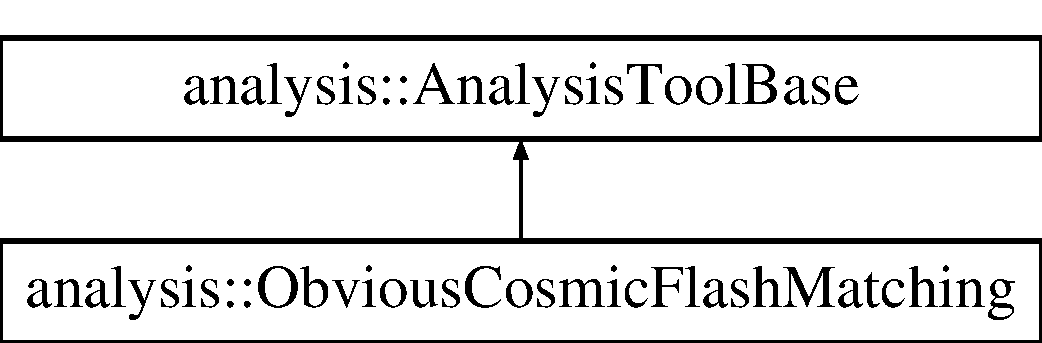
\includegraphics[height=2.000000cm]{classanalysis_1_1ObviousCosmicFlashMatching}
\end{center}
\end{figure}
\subsection*{Public Member Functions}
\begin{DoxyCompactItemize}
\item 
\hyperlink{classanalysis_1_1ObviousCosmicFlashMatching_a83be7e60be73f5d4297ae617b5f7c70f}{Obvious\-Cosmic\-Flash\-Matching} (const fhicl\-::\-Parameter\-Set \&pset)
\begin{DoxyCompactList}\small\item\em Constructor. \end{DoxyCompactList}\item 
\hypertarget{classanalysis_1_1ObviousCosmicFlashMatching_a130b94ad72bcc4157edc74e53d26d1c6}{\hyperlink{classanalysis_1_1ObviousCosmicFlashMatching_a130b94ad72bcc4157edc74e53d26d1c6}{$\sim$\-Obvious\-Cosmic\-Flash\-Matching} ()}\label{classanalysis_1_1ObviousCosmicFlashMatching_a130b94ad72bcc4157edc74e53d26d1c6}

\begin{DoxyCompactList}\small\item\em Destructor. \end{DoxyCompactList}\item 
void \hyperlink{classanalysis_1_1ObviousCosmicFlashMatching_a1ab342bc97749873a4e3118ab541af86}{configure} (fhicl\-::\-Parameter\-Set const \&pset)
\item 
void \hyperlink{classanalysis_1_1ObviousCosmicFlashMatching_ac2abf5075cbd03ffde102e14ae260707}{analyze\-Event} (art\-::\-Event const \&e, bool f\-Data) override
\begin{DoxyCompactList}\small\item\em Analysis function. \end{DoxyCompactList}\item 
\hypertarget{classanalysis_1_1ObviousCosmicFlashMatching_adbdb066be56f971dc6dc4191a56b5693}{void \hyperlink{classanalysis_1_1ObviousCosmicFlashMatching_adbdb066be56f971dc6dc4191a56b5693}{analyze\-Slice} (art\-::\-Event const \&e, std\-::vector$<$ Proxy\-Pfp\-Elem\-\_\-t $>$ \&slice\-\_\-pfp\-\_\-v, bool f\-Data, bool selected) override}\label{classanalysis_1_1ObviousCosmicFlashMatching_adbdb066be56f971dc6dc4191a56b5693}

\begin{DoxyCompactList}\small\item\em Analyze slice. \end{DoxyCompactList}\item 
\hypertarget{classanalysis_1_1ObviousCosmicFlashMatching_ae3cb2192a7edde6b72b18f172f012c12}{void \hyperlink{classanalysis_1_1ObviousCosmicFlashMatching_ae3cb2192a7edde6b72b18f172f012c12}{set\-Branches} (T\-Tree $\ast$\-\_\-tree) override}\label{classanalysis_1_1ObviousCosmicFlashMatching_ae3cb2192a7edde6b72b18f172f012c12}

\begin{DoxyCompactList}\small\item\em set branches for T\-Tree \end{DoxyCompactList}\item 
\hypertarget{classanalysis_1_1ObviousCosmicFlashMatching_a8de3a3d2c1688baf8ba9b08dc8566498}{void \hyperlink{classanalysis_1_1ObviousCosmicFlashMatching_a8de3a3d2c1688baf8ba9b08dc8566498}{reset\-T\-Tree} (T\-Tree $\ast$\-\_\-tree) override}\label{classanalysis_1_1ObviousCosmicFlashMatching_a8de3a3d2c1688baf8ba9b08dc8566498}

\begin{DoxyCompactList}\small\item\em reset ttree branches \end{DoxyCompactList}\end{DoxyCompactItemize}
\subsection*{Private Member Functions}
\begin{DoxyCompactItemize}
\item 
\hypertarget{classanalysis_1_1ObviousCosmicFlashMatching_a6a39083532d8b742b9f490d99c8f6ba2}{void {\bfseries Add\-Daughters} (const art\-::\-Ptr$<$ recob\-::\-P\-F\-Particle $>$ \&pfp\-\_\-ptr, const art\-::\-Valid\-Handle$<$ std\-::vector$<$ recob\-::\-P\-F\-Particle $>$ $>$ \&pfp\-\_\-h, std\-::vector$<$ art\-::\-Ptr$<$ recob\-::\-P\-F\-Particle $>$ $>$ \&pfp\-\_\-v)}\label{classanalysis_1_1ObviousCosmicFlashMatching_a6a39083532d8b742b9f490d99c8f6ba2}

\item 
\hypertarget{classanalysis_1_1ObviousCosmicFlashMatching_a4eaa251b09b9ede8ddf15abfe54acb5d}{bool {\bfseries Track\-In\-Time} (const art\-::\-Ptr$<$ recob\-::\-Track $>$ \&pfp\-\_\-track\-\_\-assn\-\_\-v)}\label{classanalysis_1_1ObviousCosmicFlashMatching_a4eaa251b09b9ede8ddf15abfe54acb5d}

\end{DoxyCompactItemize}
\subsection*{Private Attributes}
\begin{DoxyCompactItemize}
\item 
\hypertarget{classanalysis_1_1ObviousCosmicFlashMatching_a83588accbd48ba35aeadafeb9d4e40b0}{art\-::\-Input\-Tag {\bfseries f\-P\-F\-Pproducer}}\label{classanalysis_1_1ObviousCosmicFlashMatching_a83588accbd48ba35aeadafeb9d4e40b0}

\item 
\hypertarget{classanalysis_1_1ObviousCosmicFlashMatching_a0de5fce6b932c6f067e9bd29e67ba66c}{art\-::\-Input\-Tag {\bfseries f\-Space\-Pointproducer}}\label{classanalysis_1_1ObviousCosmicFlashMatching_a0de5fce6b932c6f067e9bd29e67ba66c}

\item 
\hypertarget{classanalysis_1_1ObviousCosmicFlashMatching_a216ba00d70eb9c1efa2650899c07d08a}{float {\bfseries \-\_\-obvious\-\_\-flashmatch\-\_\-score}}\label{classanalysis_1_1ObviousCosmicFlashMatching_a216ba00d70eb9c1efa2650899c07d08a}

\item 
\hypertarget{classanalysis_1_1ObviousCosmicFlashMatching_a6de846555ca701bb3736814e3b7fcdd0}{float {\bfseries \-\_\-neutrino\-\_\-score}}\label{classanalysis_1_1ObviousCosmicFlashMatching_a6de846555ca701bb3736814e3b7fcdd0}

\item 
\hypertarget{classanalysis_1_1ObviousCosmicFlashMatching_abde344e78325b762b59e7fef1512b57a}{float {\bfseries \-\_\-score}}\label{classanalysis_1_1ObviousCosmicFlashMatching_abde344e78325b762b59e7fef1512b57a}

\item 
\hypertarget{classanalysis_1_1ObviousCosmicFlashMatching_af0525e226ace7b7e9267d52f1813d008}{int {\bfseries \-\_\-obvious}}\label{classanalysis_1_1ObviousCosmicFlashMatching_af0525e226ace7b7e9267d52f1813d008}

\item 
\hypertarget{classanalysis_1_1ObviousCosmicFlashMatching_aac4450d61a632ccafb9399a51f0f0965}{int {\bfseries \-\_\-obvious\-\_\-cosmics}}\label{classanalysis_1_1ObviousCosmicFlashMatching_aac4450d61a632ccafb9399a51f0f0965}

\item 
\hypertarget{classanalysis_1_1ObviousCosmicFlashMatching_a1695f5108b8b9ffe1d6019912a23f69f}{float {\bfseries \-\_\-obvious\-\_\-trklen}}\label{classanalysis_1_1ObviousCosmicFlashMatching_a1695f5108b8b9ffe1d6019912a23f69f}

\item 
\hypertarget{classanalysis_1_1ObviousCosmicFlashMatching_a552228843e9c68e59327cbeec9f18b0f}{float {\bfseries \-\_\-obvious\-\_\-startx}}\label{classanalysis_1_1ObviousCosmicFlashMatching_a552228843e9c68e59327cbeec9f18b0f}

\item 
\hypertarget{classanalysis_1_1ObviousCosmicFlashMatching_a9efa838d3025aed6f83e665d6ab8032e}{float {\bfseries \-\_\-obvious\-\_\-starty}}\label{classanalysis_1_1ObviousCosmicFlashMatching_a9efa838d3025aed6f83e665d6ab8032e}

\item 
\hypertarget{classanalysis_1_1ObviousCosmicFlashMatching_a128e53a7cbe7724d8a2a7f66c0fe6441}{float {\bfseries \-\_\-obvious\-\_\-startz}}\label{classanalysis_1_1ObviousCosmicFlashMatching_a128e53a7cbe7724d8a2a7f66c0fe6441}

\item 
\hypertarget{classanalysis_1_1ObviousCosmicFlashMatching_a9302fa7f0150051d458ce920322d494d}{float {\bfseries \-\_\-obvious\-\_\-endx}}\label{classanalysis_1_1ObviousCosmicFlashMatching_a9302fa7f0150051d458ce920322d494d}

\item 
\hypertarget{classanalysis_1_1ObviousCosmicFlashMatching_ab3c098b4bb9ee7f207e947832bbca631}{float {\bfseries \-\_\-obvious\-\_\-endy}}\label{classanalysis_1_1ObviousCosmicFlashMatching_ab3c098b4bb9ee7f207e947832bbca631}

\item 
\hypertarget{classanalysis_1_1ObviousCosmicFlashMatching_add557e72442a1b02896c93b8b8c10a41}{float {\bfseries \-\_\-obvious\-\_\-endz}}\label{classanalysis_1_1ObviousCosmicFlashMatching_add557e72442a1b02896c93b8b8c10a41}

\item 
\hypertarget{classanalysis_1_1ObviousCosmicFlashMatching_ae29dc413c11e938d1d48f3929b80575b}{std\-::vector$<$ float $>$ {\bfseries \-\_\-pe\-Spectrum}}\label{classanalysis_1_1ObviousCosmicFlashMatching_ae29dc413c11e938d1d48f3929b80575b}

\item 
\hypertarget{classanalysis_1_1ObviousCosmicFlashMatching_a4851858c7c539f65cfee32fe84fe6b37}{std\-::vector$<$ float $>$ {\bfseries \-\_\-pe\-Hypothesis}}\label{classanalysis_1_1ObviousCosmicFlashMatching_a4851858c7c539f65cfee32fe84fe6b37}

\item 
\hypertarget{classanalysis_1_1ObviousCosmicFlashMatching_a65f21e28e97d83c884fe4122def4319f}{std\-::vector$<$ float $>$ {\bfseries \-\_\-pe\-Hypothesis\-Nu}}\label{classanalysis_1_1ObviousCosmicFlashMatching_a65f21e28e97d83c884fe4122def4319f}

\item 
\hypertarget{classanalysis_1_1ObviousCosmicFlashMatching_af9ea95ef3df8a9f78c137a9c4f7eda3a}{std\-::vector$<$ float $>$ {\bfseries \-\_\-pe\-Hypothesis\-Cosmic}}\label{classanalysis_1_1ObviousCosmicFlashMatching_af9ea95ef3df8a9f78c137a9c4f7eda3a}

\item 
\hypertarget{classanalysis_1_1ObviousCosmicFlashMatching_a55b71fbfeae7daaf9bf673b7565503cc}{std\-::map$<$ unsigned int, \\*
unsigned int $>$ {\bfseries \-\_\-pfpmap}}\label{classanalysis_1_1ObviousCosmicFlashMatching_a55b71fbfeae7daaf9bf673b7565503cc}

\item 
\hypertarget{classanalysis_1_1ObviousCosmicFlashMatching_a6142bc3956c3c5463c7146a3053f9025}{std\-::unique\-\_\-ptr\\*
$<$ \hyperlink{classflashmatch_1_1FlashMatchingToolBase}{flashmatch\-::\-Flash\-Matching\-Tool\-Base} $>$ \hyperlink{classanalysis_1_1ObviousCosmicFlashMatching_a6142bc3956c3c5463c7146a3053f9025}{\-\_\-flashmatch\-Tool}}\label{classanalysis_1_1ObviousCosmicFlashMatching_a6142bc3956c3c5463c7146a3053f9025}

\begin{DoxyCompactList}\small\item\em The slice id tool. \end{DoxyCompactList}\end{DoxyCompactItemize}


\subsection{Constructor \& Destructor Documentation}
\hypertarget{classanalysis_1_1ObviousCosmicFlashMatching_a83be7e60be73f5d4297ae617b5f7c70f}{\index{analysis\-::\-Obvious\-Cosmic\-Flash\-Matching@{analysis\-::\-Obvious\-Cosmic\-Flash\-Matching}!Obvious\-Cosmic\-Flash\-Matching@{Obvious\-Cosmic\-Flash\-Matching}}
\index{Obvious\-Cosmic\-Flash\-Matching@{Obvious\-Cosmic\-Flash\-Matching}!analysis::ObviousCosmicFlashMatching@{analysis\-::\-Obvious\-Cosmic\-Flash\-Matching}}
\subsubsection[{Obvious\-Cosmic\-Flash\-Matching}]{\setlength{\rightskip}{0pt plus 5cm}analysis\-::\-Obvious\-Cosmic\-Flash\-Matching\-::\-Obvious\-Cosmic\-Flash\-Matching (
\begin{DoxyParamCaption}
\item[{const fhicl\-::\-Parameter\-Set \&}]{p}
\end{DoxyParamCaption}
)}}\label{classanalysis_1_1ObviousCosmicFlashMatching_a83be7e60be73f5d4297ae617b5f7c70f}


Constructor. 


\begin{DoxyParams}{Parameters}
{\em pset} & Constructor.\\
\hline
\end{DoxyParams}
Arguments\-:

pset -\/ Fcl parameters. 

\subsection{Member Function Documentation}
\hypertarget{classanalysis_1_1ObviousCosmicFlashMatching_ac2abf5075cbd03ffde102e14ae260707}{\index{analysis\-::\-Obvious\-Cosmic\-Flash\-Matching@{analysis\-::\-Obvious\-Cosmic\-Flash\-Matching}!analyze\-Event@{analyze\-Event}}
\index{analyze\-Event@{analyze\-Event}!analysis::ObviousCosmicFlashMatching@{analysis\-::\-Obvious\-Cosmic\-Flash\-Matching}}
\subsubsection[{analyze\-Event}]{\setlength{\rightskip}{0pt plus 5cm}void analysis\-::\-Obvious\-Cosmic\-Flash\-Matching\-::analyze\-Event (
\begin{DoxyParamCaption}
\item[{art\-::\-Event const \&}]{e, }
\item[{bool}]{f\-Data}
\end{DoxyParamCaption}
)\hspace{0.3cm}{\ttfamily [override]}, {\ttfamily [virtual]}}}\label{classanalysis_1_1ObviousCosmicFlashMatching_ac2abf5075cbd03ffde102e14ae260707}


Analysis function. 

Reconfigure method.

Arguments\-:

pset -\/ Fcl parameter set. 

Implements \hyperlink{classanalysis_1_1AnalysisToolBase_ad5079f85c78e6c40f70ebf4ee31f5600}{analysis\-::\-Analysis\-Tool\-Base}.

\hypertarget{classanalysis_1_1ObviousCosmicFlashMatching_a1ab342bc97749873a4e3118ab541af86}{\index{analysis\-::\-Obvious\-Cosmic\-Flash\-Matching@{analysis\-::\-Obvious\-Cosmic\-Flash\-Matching}!configure@{configure}}
\index{configure@{configure}!analysis::ObviousCosmicFlashMatching@{analysis\-::\-Obvious\-Cosmic\-Flash\-Matching}}
\subsubsection[{configure}]{\setlength{\rightskip}{0pt plus 5cm}void analysis\-::\-Obvious\-Cosmic\-Flash\-Matching\-::configure (
\begin{DoxyParamCaption}
\item[{fhicl\-::\-Parameter\-Set const \&}]{p}
\end{DoxyParamCaption}
)}}\label{classanalysis_1_1ObviousCosmicFlashMatching_a1ab342bc97749873a4e3118ab541af86}
Reconfigure method.

Arguments\-:

pset -\/ Fcl parameter set. 

The documentation for this class was generated from the following file\-:\begin{DoxyCompactItemize}
\item 
/home/travis/build/ubneutrinos/searchingfornues/\-Selection/\-Analysis\-Tools/Obvious\-Cosmic\-Flash\-Matching\-\_\-tool.\-cc\end{DoxyCompactItemize}

\hypertarget{classflashmatch_1_1FlashMatchingTool_1_1OutputEvent}{\section{flashmatch\-:\-:Flash\-Matching\-Tool\-:\-:Output\-Event Class Reference}
\label{classflashmatch_1_1FlashMatchingTool_1_1OutputEvent}\index{flashmatch\-::\-Flash\-Matching\-Tool\-::\-Output\-Event@{flashmatch\-::\-Flash\-Matching\-Tool\-::\-Output\-Event}}
}


Class to hold information about the event for monitoring.  


\subsection*{Public Member Functions}
\begin{DoxyCompactItemize}
\item 
void \hyperlink{classflashmatch_1_1FlashMatchingTool_1_1OutputEvent_a8c2978d692f26862189e5285c0a5471d}{Reset} (const art\-::\-Event \&event)
\begin{DoxyCompactList}\small\item\em Reset the variables to default dummy values. \end{DoxyCompactList}\end{DoxyCompactItemize}
\subsection*{Public Attributes}
\begin{DoxyCompactItemize}
\item 
\hypertarget{classflashmatch_1_1FlashMatchingTool_1_1OutputEvent_a3b067cad07e0b058f5ec0188ddac0c1a}{int \hyperlink{classflashmatch_1_1FlashMatchingTool_1_1OutputEvent_a3b067cad07e0b058f5ec0188ddac0c1a}{m\-\_\-run}}\label{classflashmatch_1_1FlashMatchingTool_1_1OutputEvent_a3b067cad07e0b058f5ec0188ddac0c1a}

\begin{DoxyCompactList}\small\item\em The run number. \end{DoxyCompactList}\item 
\hypertarget{classflashmatch_1_1FlashMatchingTool_1_1OutputEvent_a140221d58b161a1548eea541b1615c78}{int \hyperlink{classflashmatch_1_1FlashMatchingTool_1_1OutputEvent_a140221d58b161a1548eea541b1615c78}{m\-\_\-sub\-Run}}\label{classflashmatch_1_1FlashMatchingTool_1_1OutputEvent_a140221d58b161a1548eea541b1615c78}

\begin{DoxyCompactList}\small\item\em The sub\-Run number. \end{DoxyCompactList}\item 
\hypertarget{classflashmatch_1_1FlashMatchingTool_1_1OutputEvent_ae1571944112e9926ad96571fe67317eb}{int \hyperlink{classflashmatch_1_1FlashMatchingTool_1_1OutputEvent_ae1571944112e9926ad96571fe67317eb}{m\-\_\-event}}\label{classflashmatch_1_1FlashMatchingTool_1_1OutputEvent_ae1571944112e9926ad96571fe67317eb}

\begin{DoxyCompactList}\small\item\em The event number. \end{DoxyCompactList}\item 
\hypertarget{classflashmatch_1_1FlashMatchingTool_1_1OutputEvent_ac70900d643ff65bddf250825e31e37c2}{int \hyperlink{classflashmatch_1_1FlashMatchingTool_1_1OutputEvent_ac70900d643ff65bddf250825e31e37c2}{m\-\_\-n\-Flashes}}\label{classflashmatch_1_1FlashMatchingTool_1_1OutputEvent_ac70900d643ff65bddf250825e31e37c2}

\begin{DoxyCompactList}\small\item\em The number of flashes. \end{DoxyCompactList}\item 
\hypertarget{classflashmatch_1_1FlashMatchingTool_1_1OutputEvent_a0815b7c52a77a59a5a95f39276a113e3}{int \hyperlink{classflashmatch_1_1FlashMatchingTool_1_1OutputEvent_a0815b7c52a77a59a5a95f39276a113e3}{m\-\_\-n\-Flashes\-In\-Beam\-Window}}\label{classflashmatch_1_1FlashMatchingTool_1_1OutputEvent_a0815b7c52a77a59a5a95f39276a113e3}

\begin{DoxyCompactList}\small\item\em The number of flashes in the beam window. \end{DoxyCompactList}\item 
\hypertarget{classflashmatch_1_1FlashMatchingTool_1_1OutputEvent_a9e92162c1cc3f01035790f16a10fa1a3}{bool \hyperlink{classflashmatch_1_1FlashMatchingTool_1_1OutputEvent_a9e92162c1cc3f01035790f16a10fa1a3}{m\-\_\-has\-Beam\-Flash}}\label{classflashmatch_1_1FlashMatchingTool_1_1OutputEvent_a9e92162c1cc3f01035790f16a10fa1a3}

\begin{DoxyCompactList}\small\item\em If a beam flash was found. \end{DoxyCompactList}\item 
\hypertarget{classflashmatch_1_1FlashMatchingTool_1_1OutputEvent_aa7f53bbb1437cf37dd0b309583ab17fd}{int \hyperlink{classflashmatch_1_1FlashMatchingTool_1_1OutputEvent_aa7f53bbb1437cf37dd0b309583ab17fd}{m\-\_\-n\-Slices}}\label{classflashmatch_1_1FlashMatchingTool_1_1OutputEvent_aa7f53bbb1437cf37dd0b309583ab17fd}

\begin{DoxyCompactList}\small\item\em The number of slices. \end{DoxyCompactList}\item 
\hypertarget{classflashmatch_1_1FlashMatchingTool_1_1OutputEvent_a1082644564c236e914d79039d09aa4c6}{int \hyperlink{classflashmatch_1_1FlashMatchingTool_1_1OutputEvent_a1082644564c236e914d79039d09aa4c6}{m\-\_\-n\-Slices\-After\-Precuts}}\label{classflashmatch_1_1FlashMatchingTool_1_1OutputEvent_a1082644564c236e914d79039d09aa4c6}

\begin{DoxyCompactList}\small\item\em The number of slices remaining after the preselection cuts. \end{DoxyCompactList}\item 
\hypertarget{classflashmatch_1_1FlashMatchingTool_1_1OutputEvent_a7f5aaa5a8baaeacce19ffd2e9efdf92f}{bool \hyperlink{classflashmatch_1_1FlashMatchingTool_1_1OutputEvent_a7f5aaa5a8baaeacce19ffd2e9efdf92f}{m\-\_\-found\-A\-Target\-Slice}}\label{classflashmatch_1_1FlashMatchingTool_1_1OutputEvent_a7f5aaa5a8baaeacce19ffd2e9efdf92f}

\begin{DoxyCompactList}\small\item\em If a slice was identified as the target (neutrino) \end{DoxyCompactList}\item 
\hypertarget{classflashmatch_1_1FlashMatchingTool_1_1OutputEvent_a840f143d067c5065ecbf8f7e0397bacf}{int \hyperlink{classflashmatch_1_1FlashMatchingTool_1_1OutputEvent_a840f143d067c5065ecbf8f7e0397bacf}{m\-\_\-target\-Slice\-Method}}\label{classflashmatch_1_1FlashMatchingTool_1_1OutputEvent_a840f143d067c5065ecbf8f7e0397bacf}

\begin{DoxyCompactList}\small\item\em 0\-: only one slice passed precuts, 1\-: has best toposcore, 2\-: has best flashmatchscore \end{DoxyCompactList}\end{DoxyCompactItemize}


\subsection{Detailed Description}
Class to hold information about the event for monitoring. 

\subsection{Member Function Documentation}
\hypertarget{classflashmatch_1_1FlashMatchingTool_1_1OutputEvent_a8c2978d692f26862189e5285c0a5471d}{\index{flashmatch\-::\-Flash\-Matching\-Tool\-::\-Output\-Event@{flashmatch\-::\-Flash\-Matching\-Tool\-::\-Output\-Event}!Reset@{Reset}}
\index{Reset@{Reset}!flashmatch::FlashMatchingTool::OutputEvent@{flashmatch\-::\-Flash\-Matching\-Tool\-::\-Output\-Event}}
\subsubsection[{Reset}]{\setlength{\rightskip}{0pt plus 5cm}void flashmatch\-::\-Flash\-Matching\-Tool\-::\-Output\-Event\-::\-Reset (
\begin{DoxyParamCaption}
\item[{const art\-::\-Event \&}]{event}
\end{DoxyParamCaption}
)\hspace{0.3cm}{\ttfamily [inline]}}}\label{classflashmatch_1_1FlashMatchingTool_1_1OutputEvent_a8c2978d692f26862189e5285c0a5471d}


Reset the variables to default dummy values. 


\begin{DoxyParams}{Parameters}
{\em event} & the art event \\
\hline
\end{DoxyParams}


The documentation for this class was generated from the following file\-:\begin{DoxyCompactItemize}
\item 
/home/travis/build/ubneutrinos/searchingfornues/\-Flash\-Matching/Flash\-Matching\-Tool\-\_\-tool.\-cc\end{DoxyCompactItemize}

\hypertarget{classselection_1_1Pi0Selection}{}\section{selection\+:\+:Pi0\+Selection Class Reference}
\label{classselection_1_1Pi0Selection}\index{selection\+::\+Pi0\+Selection@{selection\+::\+Pi0\+Selection}}
Inheritance diagram for selection\+:\+:Pi0\+Selection\+:\begin{figure}[H]
\begin{center}
\leavevmode
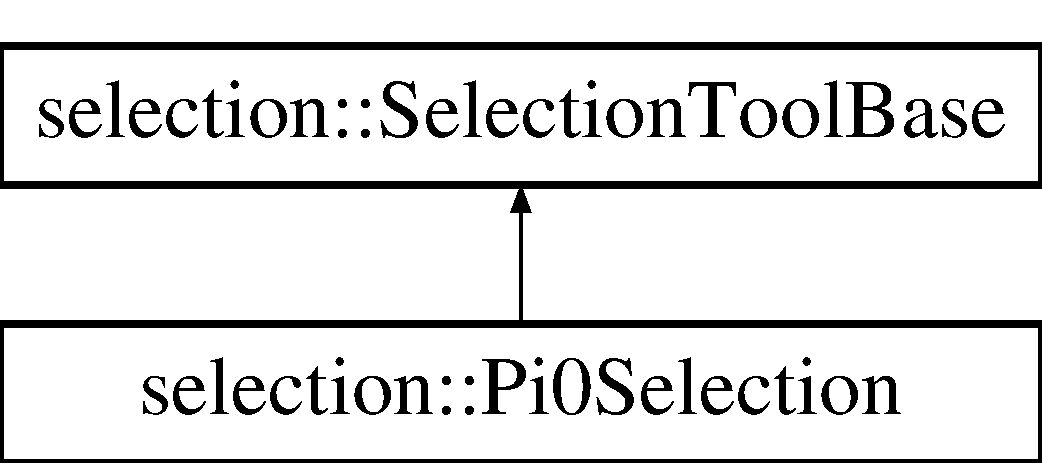
\includegraphics[height=2.000000cm]{classselection_1_1Pi0Selection}
\end{center}
\end{figure}
\subsection*{Public Member Functions}
\begin{DoxyCompactItemize}
\item 
\hyperlink{classselection_1_1Pi0Selection_a96b0ec7f6597fa143e9478a6e71f5e76}{Pi0\+Selection} (const fhicl\+::\+Parameter\+Set \&pset)
\begin{DoxyCompactList}\small\item\em Constructor. \end{DoxyCompactList}\item 
\hyperlink{classselection_1_1Pi0Selection_ad691918c955035275406f16331ba0631}{$\sim$\+Pi0\+Selection} ()\hypertarget{classselection_1_1Pi0Selection_ad691918c955035275406f16331ba0631}{}\label{classselection_1_1Pi0Selection_ad691918c955035275406f16331ba0631}

\begin{DoxyCompactList}\small\item\em Destructor. \end{DoxyCompactList}\item 
void \hyperlink{classselection_1_1Pi0Selection_a0f845ce49bdafea967214a0ac981ab87}{configure} (fhicl\+::\+Parameter\+Set const \&pset)
\item 
bool \hyperlink{classselection_1_1Pi0Selection_a1efba82b7ec3c2e18a48a98605720009}{select\+Event} (art\+::\+Event const \&e, const std\+::vector$<$ Proxy\+Pfp\+Elem\+\_\+t $>$ \&pfp\+\_\+pxy\+\_\+v)
\begin{DoxyCompactList}\small\item\em Selection function. \end{DoxyCompactList}\item 
void \hyperlink{classselection_1_1Pi0Selection_ab5e8ca896ae6aa1e2e37c437a2b29016}{set\+Branches} (T\+Tree $\ast$\+\_\+tree)
\begin{DoxyCompactList}\small\item\em set branches for T\+Tree \end{DoxyCompactList}\item 
void \hyperlink{classselection_1_1Pi0Selection_a70d28f2b466a735199640520c22fa725}{reset\+T\+Tree} (T\+Tree $\ast$\+\_\+tree)\hypertarget{classselection_1_1Pi0Selection_a70d28f2b466a735199640520c22fa725}{}\label{classselection_1_1Pi0Selection_a70d28f2b466a735199640520c22fa725}

\begin{DoxyCompactList}\small\item\em reset ttree branches \end{DoxyCompactList}\end{DoxyCompactItemize}
\subsection*{Private Member Functions}
\begin{DoxyCompactItemize}
\item 
void {\bfseries Track\+Fitd\+Edx} (const searchingfornues\+::\+Proxy\+Calo\+Elem\+\_\+t \&trk, float \&dedxU, float \&dedxV, float \&dedxY)\hypertarget{classselection_1_1Pi0Selection_ae4c04e3355249e513c5096cc8381317c}{}\label{classselection_1_1Pi0Selection_ae4c04e3355249e513c5096cc8381317c}

\item 
std\+::pair$<$ double, double $>$ {\bfseries Vtx\+Compatibility} (const T\+Vector3 \&nuvtx, const T\+Vector3 \&shrvtx, const T\+Vector3 \&shrdir)\hypertarget{classselection_1_1Pi0Selection_ad5dca90018e57209bfb37d07cfb352eb}{}\label{classselection_1_1Pi0Selection_ad5dca90018e57209bfb37d07cfb352eb}

\item 
float {\bfseries Get\+Track\+Shower\+Score} (const Proxy\+Pfp\+Elem\+\_\+t \&pfp\+\_\+pxy)\hypertarget{classselection_1_1Pi0Selection_a4605f0795f90e5bab0053b9798b53527}{}\label{classselection_1_1Pi0Selection_a4605f0795f90e5bab0053b9798b53527}

\item 
{\footnotesize template$<$typename T $>$ }\\float \hyperlink{classselection_1_1Pi0Selection_ada49763ed62a370288aa41eb67eb2c81}{P\+F\+P\+Energy} (const T \&ass\+\_\+clus\+\_\+v)\hypertarget{classselection_1_1Pi0Selection_ada49763ed62a370288aa41eb67eb2c81}{}\label{classselection_1_1Pi0Selection_ada49763ed62a370288aa41eb67eb2c81}

\begin{DoxyCompactList}\small\item\em calculate P\+FP energy based on hits associated to clusters \end{DoxyCompactList}\item 
void \hyperlink{classselection_1_1Pi0Selection_aa56e851c27c26dd695a9a831ed693401}{Read\+Truth} (art\+::\+Event const \&e)\hypertarget{classselection_1_1Pi0Selection_aa56e851c27c26dd695a9a831ed693401}{}\label{classselection_1_1Pi0Selection_aa56e851c27c26dd695a9a831ed693401}

\begin{DoxyCompactList}\small\item\em read truth info associated to pi0 \end{DoxyCompactList}\item 
void {\bfseries Reset} ()\hypertarget{classselection_1_1Pi0Selection_a32a8080624253e6d72b7d55526d50a42}{}\label{classselection_1_1Pi0Selection_a32a8080624253e6d72b7d55526d50a42}

\end{DoxyCompactItemize}
\subsection*{Private Attributes}
\begin{DoxyCompactItemize}
\item 
int {\bfseries \+\_\+ispi0}\hypertarget{classselection_1_1Pi0Selection_a9f109aa37438d57daab5fbfc72add978}{}\label{classselection_1_1Pi0Selection_a9f109aa37438d57daab5fbfc72add978}

\item 
T\+Vector3 {\bfseries \+\_\+mcgamma0\+\_\+mom}\hypertarget{classselection_1_1Pi0Selection_afa17ef5bcb8b94a63833779d2cb42f12}{}\label{classselection_1_1Pi0Selection_afa17ef5bcb8b94a63833779d2cb42f12}

\item 
T\+Vector3 {\bfseries \+\_\+mcgamma1\+\_\+mom}\hypertarget{classselection_1_1Pi0Selection_abd02e0c21a07605ff17dccff6511a2dd}{}\label{classselection_1_1Pi0Selection_abd02e0c21a07605ff17dccff6511a2dd}

\item 
float {\bfseries \+\_\+mcgamma0\+\_\+e}\hypertarget{classselection_1_1Pi0Selection_a7767b509d7c14df927541f174483d8ae}{}\label{classselection_1_1Pi0Selection_a7767b509d7c14df927541f174483d8ae}

\item 
float {\bfseries \+\_\+mcgamma0\+\_\+px}\hypertarget{classselection_1_1Pi0Selection_a344d50057f0e318a95bde4e569ecaaa7}{}\label{classselection_1_1Pi0Selection_a344d50057f0e318a95bde4e569ecaaa7}

\item 
float {\bfseries \+\_\+mcgamma0\+\_\+py}\hypertarget{classselection_1_1Pi0Selection_a3c2c28762a819a7bff467a26d960ab0f}{}\label{classselection_1_1Pi0Selection_a3c2c28762a819a7bff467a26d960ab0f}

\item 
float {\bfseries \+\_\+mcgamma0\+\_\+pz}\hypertarget{classselection_1_1Pi0Selection_ad3817990189174e99b4d57e3e323fd59}{}\label{classselection_1_1Pi0Selection_ad3817990189174e99b4d57e3e323fd59}

\item 
float {\bfseries \+\_\+mcgamma1\+\_\+e}\hypertarget{classselection_1_1Pi0Selection_a94983a7396fe33a47424a9c835588470}{}\label{classselection_1_1Pi0Selection_a94983a7396fe33a47424a9c835588470}

\item 
float {\bfseries \+\_\+mcgamma1\+\_\+px}\hypertarget{classselection_1_1Pi0Selection_af389391c864b618d954aee77054fc560}{}\label{classselection_1_1Pi0Selection_af389391c864b618d954aee77054fc560}

\item 
float {\bfseries \+\_\+mcgamma1\+\_\+py}\hypertarget{classselection_1_1Pi0Selection_a60fe0602f4980bfa22a997d57bb4f1e2}{}\label{classselection_1_1Pi0Selection_a60fe0602f4980bfa22a997d57bb4f1e2}

\item 
float {\bfseries \+\_\+mcgamma1\+\_\+pz}\hypertarget{classselection_1_1Pi0Selection_a5eba1408915da889a6ae0f79d170585f}{}\label{classselection_1_1Pi0Selection_a5eba1408915da889a6ae0f79d170585f}

\item 
float {\bfseries \+\_\+mcrcdot0}\hypertarget{classselection_1_1Pi0Selection_ac947a79ab609a41e711a6ef07db92ea1}{}\label{classselection_1_1Pi0Selection_ac947a79ab609a41e711a6ef07db92ea1}

\item 
float {\bfseries \+\_\+mcrcdot1}\hypertarget{classselection_1_1Pi0Selection_a953aac9aad7f28af064de412b0c67eff}{}\label{classselection_1_1Pi0Selection_a953aac9aad7f28af064de412b0c67eff}

\item 
float {\bfseries \+\_\+mcrce0}\hypertarget{classselection_1_1Pi0Selection_adaa35a245f9997e9a2caa0584c938604}{}\label{classselection_1_1Pi0Selection_adaa35a245f9997e9a2caa0584c938604}

\item 
float {\bfseries \+\_\+mcrce1}\hypertarget{classselection_1_1Pi0Selection_a38cbd53f61a0f698f037fa004f4fc57e}{}\label{classselection_1_1Pi0Selection_a38cbd53f61a0f698f037fa004f4fc57e}

\item 
int {\bfseries \+\_\+nshower}\hypertarget{classselection_1_1Pi0Selection_a49171ea13b719323289856088be76f14}{}\label{classselection_1_1Pi0Selection_a49171ea13b719323289856088be76f14}

\item 
int {\bfseries \+\_\+ntrack}\hypertarget{classselection_1_1Pi0Selection_abaff27fd2e31e5aede9d561e47b89548}{}\label{classselection_1_1Pi0Selection_abaff27fd2e31e5aede9d561e47b89548}

\item 
int {\bfseries \+\_\+ngamma}\hypertarget{classselection_1_1Pi0Selection_a1d84f7559c912c34b140fbdc9370d700}{}\label{classselection_1_1Pi0Selection_a1d84f7559c912c34b140fbdc9370d700}

\item 
float {\bfseries \+\_\+radlen1}\hypertarget{classselection_1_1Pi0Selection_a773cea8619973a768cd5e07dcba6ef98}{}\label{classselection_1_1Pi0Selection_a773cea8619973a768cd5e07dcba6ef98}

\item 
float {\bfseries \+\_\+radlen2}\hypertarget{classselection_1_1Pi0Selection_a69fe4916f3a1934461f0cdddb6f3a9bb}{}\label{classselection_1_1Pi0Selection_a69fe4916f3a1934461f0cdddb6f3a9bb}

\item 
float {\bfseries \+\_\+dot1}\hypertarget{classselection_1_1Pi0Selection_ac9a1962d0aace5e61d9821ca4e58d220}{}\label{classselection_1_1Pi0Selection_ac9a1962d0aace5e61d9821ca4e58d220}

\item 
float {\bfseries \+\_\+dot2}\hypertarget{classselection_1_1Pi0Selection_ac9cf7e3add0f9f8bf0be25f8ab365179}{}\label{classselection_1_1Pi0Selection_ac9cf7e3add0f9f8bf0be25f8ab365179}

\item 
float {\bfseries \+\_\+energy1\+\_\+Y}\hypertarget{classselection_1_1Pi0Selection_aa1b9f4db070a0d2fe22463be23690a09}{}\label{classselection_1_1Pi0Selection_aa1b9f4db070a0d2fe22463be23690a09}

\item 
float {\bfseries \+\_\+energy2\+\_\+Y}\hypertarget{classselection_1_1Pi0Selection_a61c64007f6a07349b69f469ef25cb1d2}{}\label{classselection_1_1Pi0Selection_a61c64007f6a07349b69f469ef25cb1d2}

\item 
float {\bfseries \+\_\+dedx1\+\_\+Y}\hypertarget{classselection_1_1Pi0Selection_ae797a0683808220b2e2533a727024207}{}\label{classselection_1_1Pi0Selection_ae797a0683808220b2e2533a727024207}

\item 
float {\bfseries \+\_\+dedx2\+\_\+Y}\hypertarget{classselection_1_1Pi0Selection_a9f73f2c89341782ce82312af0e56d34b}{}\label{classselection_1_1Pi0Selection_a9f73f2c89341782ce82312af0e56d34b}

\item 
float {\bfseries \+\_\+dedx1\+\_\+fit\+\_\+Y}\hypertarget{classselection_1_1Pi0Selection_ad19dbe5a8c043e1bdac735d2a912c6c1}{}\label{classselection_1_1Pi0Selection_ad19dbe5a8c043e1bdac735d2a912c6c1}

\item 
float {\bfseries \+\_\+dedx2\+\_\+fit\+\_\+Y}\hypertarget{classselection_1_1Pi0Selection_af895b5498360192573e58cc616fc1086}{}\label{classselection_1_1Pi0Selection_af895b5498360192573e58cc616fc1086}

\item 
float {\bfseries \+\_\+energy1\+\_\+V}\hypertarget{classselection_1_1Pi0Selection_ae0188f6c0dbf3cf17ef4d319010832b4}{}\label{classselection_1_1Pi0Selection_ae0188f6c0dbf3cf17ef4d319010832b4}

\item 
float {\bfseries \+\_\+energy2\+\_\+V}\hypertarget{classselection_1_1Pi0Selection_acc291e37f73a8119803b7f34e7d49dbc}{}\label{classselection_1_1Pi0Selection_acc291e37f73a8119803b7f34e7d49dbc}

\item 
float {\bfseries \+\_\+dedx1\+\_\+V}\hypertarget{classselection_1_1Pi0Selection_ae9c72b46aab4eac133fda0fa4a0b6fa4}{}\label{classselection_1_1Pi0Selection_ae9c72b46aab4eac133fda0fa4a0b6fa4}

\item 
float {\bfseries \+\_\+dedx2\+\_\+V}\hypertarget{classselection_1_1Pi0Selection_aab132224486246d915411c64c50ad65e}{}\label{classselection_1_1Pi0Selection_aab132224486246d915411c64c50ad65e}

\item 
float {\bfseries \+\_\+dedx1\+\_\+fit\+\_\+V}\hypertarget{classselection_1_1Pi0Selection_a9c8c85ff5b6207f217337bb3874f4885}{}\label{classselection_1_1Pi0Selection_a9c8c85ff5b6207f217337bb3874f4885}

\item 
float {\bfseries \+\_\+dedx2\+\_\+fit\+\_\+V}\hypertarget{classselection_1_1Pi0Selection_a44e037bd7302dc645c48712f34d9c483}{}\label{classselection_1_1Pi0Selection_a44e037bd7302dc645c48712f34d9c483}

\item 
float {\bfseries \+\_\+energy1\+\_\+U}\hypertarget{classselection_1_1Pi0Selection_a0def3ec96d36c52f9eb035eeaa662f03}{}\label{classselection_1_1Pi0Selection_a0def3ec96d36c52f9eb035eeaa662f03}

\item 
float {\bfseries \+\_\+energy2\+\_\+U}\hypertarget{classselection_1_1Pi0Selection_a7451c5d1b5056ff9ce532c2f554a4dbe}{}\label{classselection_1_1Pi0Selection_a7451c5d1b5056ff9ce532c2f554a4dbe}

\item 
float {\bfseries \+\_\+dedx1\+\_\+U}\hypertarget{classselection_1_1Pi0Selection_aadb93b344c08ad4a783788e12883490f}{}\label{classselection_1_1Pi0Selection_aadb93b344c08ad4a783788e12883490f}

\item 
float {\bfseries \+\_\+dedx2\+\_\+U}\hypertarget{classselection_1_1Pi0Selection_acee8eeac54016633a186976df8f87c44}{}\label{classselection_1_1Pi0Selection_acee8eeac54016633a186976df8f87c44}

\item 
float {\bfseries \+\_\+dedx1\+\_\+fit\+\_\+U}\hypertarget{classselection_1_1Pi0Selection_a07ddc30ac5f77dc9e38fd57eadff37dd}{}\label{classselection_1_1Pi0Selection_a07ddc30ac5f77dc9e38fd57eadff37dd}

\item 
float {\bfseries \+\_\+dedx2\+\_\+fit\+\_\+U}\hypertarget{classselection_1_1Pi0Selection_a7e929dee5928aa5f4fdf630cc4700aa1}{}\label{classselection_1_1Pi0Selection_a7e929dee5928aa5f4fdf630cc4700aa1}

\item 
float {\bfseries \+\_\+shrscore1}\hypertarget{classselection_1_1Pi0Selection_abd39d26f09e8acfdae8d5bed7196f927}{}\label{classselection_1_1Pi0Selection_abd39d26f09e8acfdae8d5bed7196f927}

\item 
float {\bfseries \+\_\+shrscore2}\hypertarget{classselection_1_1Pi0Selection_aa66a2e88987f1600fe05b8c081be7c33}{}\label{classselection_1_1Pi0Selection_aa66a2e88987f1600fe05b8c081be7c33}

\item 
float {\bfseries \+\_\+gammadot}\hypertarget{classselection_1_1Pi0Selection_ac785c743e3f3d7761599eca7dc391408}{}\label{classselection_1_1Pi0Selection_ac785c743e3f3d7761599eca7dc391408}

\item 
float {\bfseries \+\_\+mass\+\_\+Y}\hypertarget{classselection_1_1Pi0Selection_a6059940bdddced57e944111f8d52fa91}{}\label{classselection_1_1Pi0Selection_a6059940bdddced57e944111f8d52fa91}

\item 
float {\bfseries \+\_\+mass\+\_\+V}\hypertarget{classselection_1_1Pi0Selection_a128bfd5ad26de833b3526d5f25d782b0}{}\label{classselection_1_1Pi0Selection_a128bfd5ad26de833b3526d5f25d782b0}

\item 
float {\bfseries \+\_\+mass\+\_\+U}\hypertarget{classselection_1_1Pi0Selection_a3cd9296bc98c1d82f82ef85377bdb966}{}\label{classselection_1_1Pi0Selection_a3cd9296bc98c1d82f82ef85377bdb966}

\item 
float {\bfseries \+\_\+rc\+\_\+vtx\+\_\+x}\hypertarget{classselection_1_1Pi0Selection_a3e8b96b42c52f4ff83ed53175821b050}{}\label{classselection_1_1Pi0Selection_a3e8b96b42c52f4ff83ed53175821b050}

\item 
float {\bfseries \+\_\+rc\+\_\+vtx\+\_\+y}\hypertarget{classselection_1_1Pi0Selection_ad2780ab5a41ec2b9658027466dcb1a61}{}\label{classselection_1_1Pi0Selection_ad2780ab5a41ec2b9658027466dcb1a61}

\item 
float {\bfseries \+\_\+rc\+\_\+vtx\+\_\+z}\hypertarget{classselection_1_1Pi0Selection_a9d468d7b86c7ce10cfe506d83ba0bc2b}{}\label{classselection_1_1Pi0Selection_a9d468d7b86c7ce10cfe506d83ba0bc2b}

\item 
bool {\bfseries \+\_\+onlyshower}\hypertarget{classselection_1_1Pi0Selection_afe28c10248c1e8422bfe433798632f5b}{}\label{classselection_1_1Pi0Selection_afe28c10248c1e8422bfe433798632f5b}

\item 
float {\bfseries \+\_\+dmin}\hypertarget{classselection_1_1Pi0Selection_a024f58d2a5b862ea9933dbca74afcb0e}{}\label{classselection_1_1Pi0Selection_a024f58d2a5b862ea9933dbca74afcb0e}

\item 
float {\bfseries \+\_\+dotmin}\hypertarget{classselection_1_1Pi0Selection_abfd819e3214069b1b5efa2bf88e96f5d}{}\label{classselection_1_1Pi0Selection_abfd819e3214069b1b5efa2bf88e96f5d}

\item 
float {\bfseries \+\_\+trkshrscore}\hypertarget{classselection_1_1Pi0Selection_aa74075888ad93d414dea65eb0ff02dc3}{}\label{classselection_1_1Pi0Selection_aa74075888ad93d414dea65eb0ff02dc3}

\item 
art\+::\+Input\+Tag {\bfseries f\+T\+R\+Kproducer}\hypertarget{classselection_1_1Pi0Selection_aa8b9b496faee370de5f3682369a32950}{}\label{classselection_1_1Pi0Selection_aa8b9b496faee370de5f3682369a32950}

\item 
art\+::\+Input\+Tag {\bfseries f\+C\+A\+Lproducer}\hypertarget{classselection_1_1Pi0Selection_a5bee48abbfcd4c25ce387740f193a5a3}{}\label{classselection_1_1Pi0Selection_a5bee48abbfcd4c25ce387740f193a5a3}

\end{DoxyCompactItemize}
\subsection*{Additional Inherited Members}


\subsection{Constructor \& Destructor Documentation}
\index{selection\+::\+Pi0\+Selection@{selection\+::\+Pi0\+Selection}!Pi0\+Selection@{Pi0\+Selection}}
\index{Pi0\+Selection@{Pi0\+Selection}!selection\+::\+Pi0\+Selection@{selection\+::\+Pi0\+Selection}}
\subsubsection[{\texorpdfstring{Pi0\+Selection(const fhicl\+::\+Parameter\+Set \&pset)}{Pi0Selection(const fhicl::ParameterSet &pset)}}]{\setlength{\rightskip}{0pt plus 5cm}selection\+::\+Pi0\+Selection\+::\+Pi0\+Selection (
\begin{DoxyParamCaption}
\item[{const fhicl\+::\+Parameter\+Set \&}]{pset}
\end{DoxyParamCaption}
)}\hypertarget{classselection_1_1Pi0Selection_a96b0ec7f6597fa143e9478a6e71f5e76}{}\label{classselection_1_1Pi0Selection_a96b0ec7f6597fa143e9478a6e71f5e76}


Constructor. 


\begin{DoxyParams}{Parameters}
{\em pset} & Constructor.\\
\hline
\end{DoxyParams}
Arguments\+:

pset -\/ Fcl parameters. 

\subsection{Member Function Documentation}
\index{selection\+::\+Pi0\+Selection@{selection\+::\+Pi0\+Selection}!configure@{configure}}
\index{configure@{configure}!selection\+::\+Pi0\+Selection@{selection\+::\+Pi0\+Selection}}
\subsubsection[{\texorpdfstring{configure(fhicl\+::\+Parameter\+Set const \&pset)}{configure(fhicl::ParameterSet const &pset)}}]{\setlength{\rightskip}{0pt plus 5cm}void selection\+::\+Pi0\+Selection\+::configure (
\begin{DoxyParamCaption}
\item[{fhicl\+::\+Parameter\+Set const \&}]{pset}
\end{DoxyParamCaption}
)}\hypertarget{classselection_1_1Pi0Selection_a0f845ce49bdafea967214a0ac981ab87}{}\label{classselection_1_1Pi0Selection_a0f845ce49bdafea967214a0ac981ab87}
Reconfigure method.

Arguments\+:

pset -\/ Fcl parameter set. \index{selection\+::\+Pi0\+Selection@{selection\+::\+Pi0\+Selection}!select\+Event@{select\+Event}}
\index{select\+Event@{select\+Event}!selection\+::\+Pi0\+Selection@{selection\+::\+Pi0\+Selection}}
\subsubsection[{\texorpdfstring{select\+Event(art\+::\+Event const \&e, const std\+::vector$<$ Proxy\+Pfp\+Elem\+\_\+t $>$ \&pfp\+\_\+pxy\+\_\+v)}{selectEvent(art::Event const &e, const std::vector< ProxyPfpElem_t > &pfp_pxy_v)}}]{\setlength{\rightskip}{0pt plus 5cm}bool selection\+::\+Pi0\+Selection\+::select\+Event (
\begin{DoxyParamCaption}
\item[{art\+::\+Event const \&}]{e, }
\item[{const std\+::vector$<$ Proxy\+Pfp\+Elem\+\_\+t $>$ \&}]{pfp\+\_\+pxy\+\_\+v}
\end{DoxyParamCaption}
)\hspace{0.3cm}{\ttfamily [virtual]}}\hypertarget{classselection_1_1Pi0Selection_a1efba82b7ec3c2e18a48a98605720009}{}\label{classselection_1_1Pi0Selection_a1efba82b7ec3c2e18a48a98605720009}


Selection function. 

select\+Event

Arguments\+:

art\+::\+Event slice track pointer vector slice shower pointer vector 

Implements \hyperlink{classselection_1_1SelectionToolBase_ab63818dac49b43418fe9eb3b8cd98c9c}{selection\+::\+Selection\+Tool\+Base}.

\index{selection\+::\+Pi0\+Selection@{selection\+::\+Pi0\+Selection}!set\+Branches@{set\+Branches}}
\index{set\+Branches@{set\+Branches}!selection\+::\+Pi0\+Selection@{selection\+::\+Pi0\+Selection}}
\subsubsection[{\texorpdfstring{set\+Branches(\+T\+Tree $\ast$\+\_\+tree)}{setBranches(TTree *_tree)}}]{\setlength{\rightskip}{0pt plus 5cm}void selection\+::\+Pi0\+Selection\+::set\+Branches (
\begin{DoxyParamCaption}
\item[{T\+Tree $\ast$}]{\+\_\+tree}
\end{DoxyParamCaption}
)\hspace{0.3cm}{\ttfamily [virtual]}}\hypertarget{classselection_1_1Pi0Selection_ab5e8ca896ae6aa1e2e37c437a2b29016}{}\label{classselection_1_1Pi0Selection_ab5e8ca896ae6aa1e2e37c437a2b29016}


set branches for T\+Tree 

cioe\textquotesingle{} $\ast$ 

Implements \hyperlink{classselection_1_1SelectionToolBase_aa97ea5e55391240d8e251dae13897996}{selection\+::\+Selection\+Tool\+Base}.



The documentation for this class was generated from the following file\+:\begin{DoxyCompactItemize}
\item 
/home/travis/build/ubneutrinos/searchingfornues/\+Selection/\+Selection\+Tools/Pi0\+Selection\+\_\+tool.\+cc\end{DoxyCompactItemize}

\hypertarget{classanalysis_1_1Pi0TruthAnalysis}{\section{analysis\-:\-:Pi0\-Truth\-Analysis Class Reference}
\label{classanalysis_1_1Pi0TruthAnalysis}\index{analysis\-::\-Pi0\-Truth\-Analysis@{analysis\-::\-Pi0\-Truth\-Analysis}}
}
Inheritance diagram for analysis\-:\-:Pi0\-Truth\-Analysis\-:\begin{figure}[H]
\begin{center}
\leavevmode
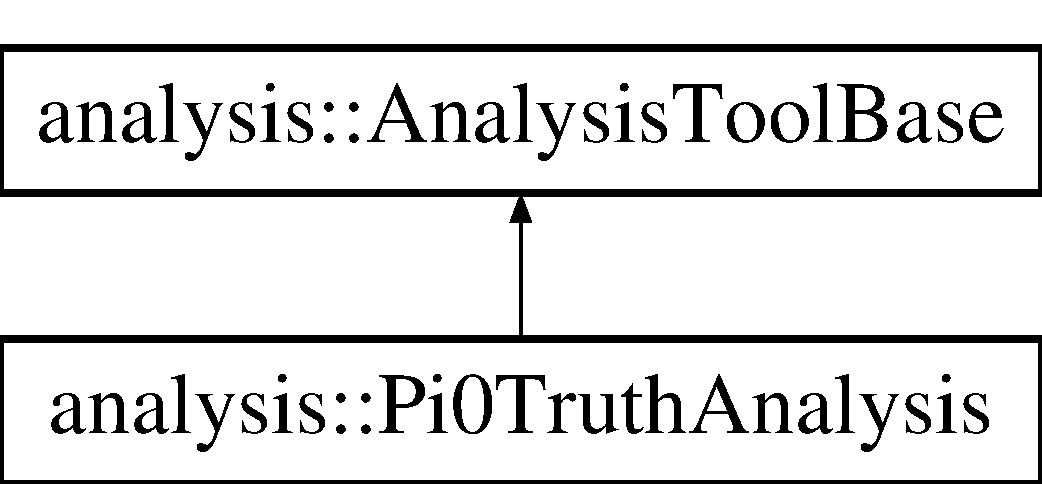
\includegraphics[height=2.000000cm]{classanalysis_1_1Pi0TruthAnalysis}
\end{center}
\end{figure}
\subsection*{Public Member Functions}
\begin{DoxyCompactItemize}
\item 
\hyperlink{classanalysis_1_1Pi0TruthAnalysis_ad58bc9cafaa153ef9c775b505d00f5ef}{Pi0\-Truth\-Analysis} (const fhicl\-::\-Parameter\-Set \&pset)
\begin{DoxyCompactList}\small\item\em Constructor. \end{DoxyCompactList}\item 
\hypertarget{classanalysis_1_1Pi0TruthAnalysis_aacb1da6bc05c5af7d13e6699c1b9112d}{\hyperlink{classanalysis_1_1Pi0TruthAnalysis_aacb1da6bc05c5af7d13e6699c1b9112d}{$\sim$\-Pi0\-Truth\-Analysis} ()}\label{classanalysis_1_1Pi0TruthAnalysis_aacb1da6bc05c5af7d13e6699c1b9112d}

\begin{DoxyCompactList}\small\item\em Destructor. \end{DoxyCompactList}\item 
void \hyperlink{classanalysis_1_1Pi0TruthAnalysis_abbbb2436e35ba1e3bc64c4fd4e07668c}{configure} (fhicl\-::\-Parameter\-Set const \&pset)
\item 
void \hyperlink{classanalysis_1_1Pi0TruthAnalysis_a07cf437c5f9d2b19b7a0ca3de447d12f}{analyze\-Event} (art\-::\-Event const \&e, bool f\-Data) override
\begin{DoxyCompactList}\small\item\em Analysis function. \end{DoxyCompactList}\item 
\hypertarget{classanalysis_1_1Pi0TruthAnalysis_a02b3f2e32b0e8097c0432bd013c0dbe1}{void \hyperlink{classanalysis_1_1Pi0TruthAnalysis_a02b3f2e32b0e8097c0432bd013c0dbe1}{analyze\-Slice} (art\-::\-Event const \&e, std\-::vector$<$ Proxy\-Pfp\-Elem\-\_\-t $>$ \&slice\-\_\-pfp\-\_\-v, bool f\-Data, bool selected) override}\label{classanalysis_1_1Pi0TruthAnalysis_a02b3f2e32b0e8097c0432bd013c0dbe1}

\begin{DoxyCompactList}\small\item\em Analyze slice. \end{DoxyCompactList}\item 
\hypertarget{classanalysis_1_1Pi0TruthAnalysis_adf40bf270a043c1eb7837460bf0e2fc5}{void \hyperlink{classanalysis_1_1Pi0TruthAnalysis_adf40bf270a043c1eb7837460bf0e2fc5}{Save\-Truth} (art\-::\-Event const \&e)}\label{classanalysis_1_1Pi0TruthAnalysis_adf40bf270a043c1eb7837460bf0e2fc5}

\begin{DoxyCompactList}\small\item\em Save truth info for event associated to neutrino. \end{DoxyCompactList}\item 
\hypertarget{classanalysis_1_1Pi0TruthAnalysis_ac802cbe61417635725355f94babe6508}{void \hyperlink{classanalysis_1_1Pi0TruthAnalysis_ac802cbe61417635725355f94babe6508}{set\-Branches} (T\-Tree $\ast$\-\_\-tree) override}\label{classanalysis_1_1Pi0TruthAnalysis_ac802cbe61417635725355f94babe6508}

\begin{DoxyCompactList}\small\item\em set branches for T\-Tree \end{DoxyCompactList}\item 
\hypertarget{classanalysis_1_1Pi0TruthAnalysis_ac2434d9167bd32874669a8ef5eccb8a7}{void \hyperlink{classanalysis_1_1Pi0TruthAnalysis_ac2434d9167bd32874669a8ef5eccb8a7}{reset\-T\-Tree} (T\-Tree $\ast$\-\_\-tree) override}\label{classanalysis_1_1Pi0TruthAnalysis_ac2434d9167bd32874669a8ef5eccb8a7}

\begin{DoxyCompactList}\small\item\em reset ttree branches \end{DoxyCompactList}\end{DoxyCompactItemize}
\subsection*{Private Attributes}
\begin{DoxyCompactItemize}
\item 
\hypertarget{classanalysis_1_1Pi0TruthAnalysis_ac0b014039b6cbb0508010c4c7fa8bc7d}{art\-::\-Input\-Tag {\bfseries f\-M\-C\-Tproducer}}\label{classanalysis_1_1Pi0TruthAnalysis_ac0b014039b6cbb0508010c4c7fa8bc7d}

\item 
\hypertarget{classanalysis_1_1Pi0TruthAnalysis_af5416caf86030ce12316cf4a9e14ff08}{art\-::\-Input\-Tag {\bfseries f\-M\-C\-Sproducer}}\label{classanalysis_1_1Pi0TruthAnalysis_af5416caf86030ce12316cf4a9e14ff08}

\item 
\hypertarget{classanalysis_1_1Pi0TruthAnalysis_af0e581e456ae211a233a448ae4a7061c}{float {\bfseries \-\_\-gamma1\-\_\-edep}}\label{classanalysis_1_1Pi0TruthAnalysis_af0e581e456ae211a233a448ae4a7061c}

\item 
\hypertarget{classanalysis_1_1Pi0TruthAnalysis_a47677e4dde1ed73f4c8758f0ef01037a}{float {\bfseries \-\_\-gamma1\-\_\-etot}}\label{classanalysis_1_1Pi0TruthAnalysis_a47677e4dde1ed73f4c8758f0ef01037a}

\item 
\hypertarget{classanalysis_1_1Pi0TruthAnalysis_af9287b9b8d319220408c0257d0d2f39b}{float {\bfseries \-\_\-gamma2\-\_\-edep}}\label{classanalysis_1_1Pi0TruthAnalysis_af9287b9b8d319220408c0257d0d2f39b}

\item 
\hypertarget{classanalysis_1_1Pi0TruthAnalysis_a43ea1af4666ab360d5acb4385fa9e1a9}{float {\bfseries \-\_\-gamma2\-\_\-etot}}\label{classanalysis_1_1Pi0TruthAnalysis_a43ea1af4666ab360d5acb4385fa9e1a9}

\item 
\hypertarget{classanalysis_1_1Pi0TruthAnalysis_a756b03fb781b7787ece0178a31b1f758}{int {\bfseries \-\_\-gamma\-\_\-parent}}\label{classanalysis_1_1Pi0TruthAnalysis_a756b03fb781b7787ece0178a31b1f758}

\item 
\hypertarget{classanalysis_1_1Pi0TruthAnalysis_a9ebf162b688fb8978eb6ff9ef137ad14}{float {\bfseries \-\_\-gamma\-\_\-edep}}\label{classanalysis_1_1Pi0TruthAnalysis_a9ebf162b688fb8978eb6ff9ef137ad14}

\item 
\hypertarget{classanalysis_1_1Pi0TruthAnalysis_acb69e34f745eee785cac4fc6c2f59c14}{float {\bfseries \-\_\-gamma\-\_\-etot}}\label{classanalysis_1_1Pi0TruthAnalysis_acb69e34f745eee785cac4fc6c2f59c14}

\item 
\hypertarget{classanalysis_1_1Pi0TruthAnalysis_a7c1335874fbaea78e02be11928d711eb}{float {\bfseries \-\_\-gamma\-\_\-dist}}\label{classanalysis_1_1Pi0TruthAnalysis_a7c1335874fbaea78e02be11928d711eb}

\item 
\hypertarget{classanalysis_1_1Pi0TruthAnalysis_a786a534ee00376b06114bba0c8a5392c}{int {\bfseries \-\_\-elec\-\_\-parent}}\label{classanalysis_1_1Pi0TruthAnalysis_a786a534ee00376b06114bba0c8a5392c}

\item 
\hypertarget{classanalysis_1_1Pi0TruthAnalysis_aed2a2cdd7fc5b1c7b17f50c7cd043e24}{float {\bfseries \-\_\-elec\-\_\-edep}}\label{classanalysis_1_1Pi0TruthAnalysis_aed2a2cdd7fc5b1c7b17f50c7cd043e24}

\item 
\hypertarget{classanalysis_1_1Pi0TruthAnalysis_a5a3b46137357fb441669ca95da1d7d69}{float {\bfseries \-\_\-elec\-\_\-etot}}\label{classanalysis_1_1Pi0TruthAnalysis_a5a3b46137357fb441669ca95da1d7d69}

\item 
\hypertarget{classanalysis_1_1Pi0TruthAnalysis_aad52612f0a988b6ff2ab0e8366eb99bc}{float {\bfseries \-\_\-elec\-\_\-dist}}\label{classanalysis_1_1Pi0TruthAnalysis_aad52612f0a988b6ff2ab0e8366eb99bc}

\end{DoxyCompactItemize}


\subsection{Constructor \& Destructor Documentation}
\hypertarget{classanalysis_1_1Pi0TruthAnalysis_ad58bc9cafaa153ef9c775b505d00f5ef}{\index{analysis\-::\-Pi0\-Truth\-Analysis@{analysis\-::\-Pi0\-Truth\-Analysis}!Pi0\-Truth\-Analysis@{Pi0\-Truth\-Analysis}}
\index{Pi0\-Truth\-Analysis@{Pi0\-Truth\-Analysis}!analysis::Pi0TruthAnalysis@{analysis\-::\-Pi0\-Truth\-Analysis}}
\subsubsection[{Pi0\-Truth\-Analysis}]{\setlength{\rightskip}{0pt plus 5cm}analysis\-::\-Pi0\-Truth\-Analysis\-::\-Pi0\-Truth\-Analysis (
\begin{DoxyParamCaption}
\item[{const fhicl\-::\-Parameter\-Set \&}]{p}
\end{DoxyParamCaption}
)}}\label{classanalysis_1_1Pi0TruthAnalysis_ad58bc9cafaa153ef9c775b505d00f5ef}


Constructor. 


\begin{DoxyParams}{Parameters}
{\em pset} & Constructor.\\
\hline
\end{DoxyParams}
Arguments\-:

pset -\/ Fcl parameters. 

\subsection{Member Function Documentation}
\hypertarget{classanalysis_1_1Pi0TruthAnalysis_a07cf437c5f9d2b19b7a0ca3de447d12f}{\index{analysis\-::\-Pi0\-Truth\-Analysis@{analysis\-::\-Pi0\-Truth\-Analysis}!analyze\-Event@{analyze\-Event}}
\index{analyze\-Event@{analyze\-Event}!analysis::Pi0TruthAnalysis@{analysis\-::\-Pi0\-Truth\-Analysis}}
\subsubsection[{analyze\-Event}]{\setlength{\rightskip}{0pt plus 5cm}void analysis\-::\-Pi0\-Truth\-Analysis\-::analyze\-Event (
\begin{DoxyParamCaption}
\item[{art\-::\-Event const \&}]{e, }
\item[{bool}]{f\-Data}
\end{DoxyParamCaption}
)\hspace{0.3cm}{\ttfamily [override]}, {\ttfamily [virtual]}}}\label{classanalysis_1_1Pi0TruthAnalysis_a07cf437c5f9d2b19b7a0ca3de447d12f}


Analysis function. 

Reconfigure method.

Arguments\-:

pset -\/ Fcl parameter set. 

Implements \hyperlink{classanalysis_1_1AnalysisToolBase_ad5079f85c78e6c40f70ebf4ee31f5600}{analysis\-::\-Analysis\-Tool\-Base}.

\hypertarget{classanalysis_1_1Pi0TruthAnalysis_abbbb2436e35ba1e3bc64c4fd4e07668c}{\index{analysis\-::\-Pi0\-Truth\-Analysis@{analysis\-::\-Pi0\-Truth\-Analysis}!configure@{configure}}
\index{configure@{configure}!analysis::Pi0TruthAnalysis@{analysis\-::\-Pi0\-Truth\-Analysis}}
\subsubsection[{configure}]{\setlength{\rightskip}{0pt plus 5cm}void analysis\-::\-Pi0\-Truth\-Analysis\-::configure (
\begin{DoxyParamCaption}
\item[{fhicl\-::\-Parameter\-Set const \&}]{p}
\end{DoxyParamCaption}
)}}\label{classanalysis_1_1Pi0TruthAnalysis_abbbb2436e35ba1e3bc64c4fd4e07668c}
Reconfigure method.

Arguments\-:

pset -\/ Fcl parameter set. 

The documentation for this class was generated from the following file\-:\begin{DoxyCompactItemize}
\item 
/home/travis/build/ubneutrinos/searchingfornues/\-Selection/\-Analysis\-Tools/Pi0\-Truth\-Analysis\-\_\-tool.\-cc\end{DoxyCompactItemize}

\hypertarget{classanalysis_1_1PMTNoise}{}\section{analysis\+:\+:P\+M\+T\+Noise Class Reference}
\label{classanalysis_1_1PMTNoise}\index{analysis\+::\+P\+M\+T\+Noise@{analysis\+::\+P\+M\+T\+Noise}}
Inheritance diagram for analysis\+:\+:P\+M\+T\+Noise\+:\begin{figure}[H]
\begin{center}
\leavevmode
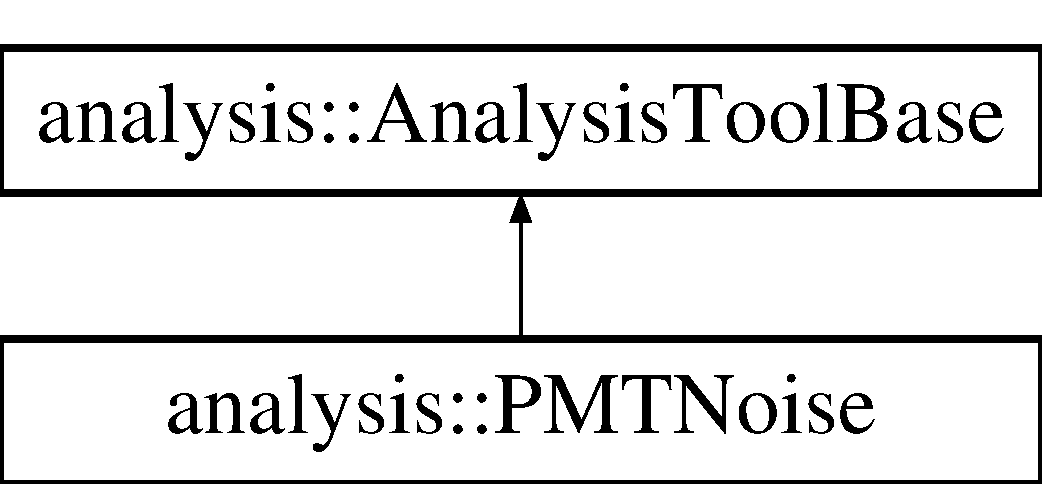
\includegraphics[height=2.000000cm]{classanalysis_1_1PMTNoise}
\end{center}
\end{figure}
\subsection*{Public Member Functions}
\begin{DoxyCompactItemize}
\item 
\hyperlink{classanalysis_1_1PMTNoise_a68d40e2ae135ebc8d8dbe3f756ee1850}{P\+M\+T\+Noise} (const fhicl\+::\+Parameter\+Set \&pset)
\begin{DoxyCompactList}\small\item\em Constructor. \end{DoxyCompactList}\item 
\hyperlink{classanalysis_1_1PMTNoise_a10c11f2bd8fd9a55ff8cb816ae23bf33}{$\sim$\+P\+M\+T\+Noise} ()\hypertarget{classanalysis_1_1PMTNoise_a10c11f2bd8fd9a55ff8cb816ae23bf33}{}\label{classanalysis_1_1PMTNoise_a10c11f2bd8fd9a55ff8cb816ae23bf33}

\begin{DoxyCompactList}\small\item\em Destructor. \end{DoxyCompactList}\item 
void \hyperlink{classanalysis_1_1PMTNoise_ac68d1b71ec42d1a6baf987d867775fd1}{configure} (fhicl\+::\+Parameter\+Set const \&pset)
\item 
void \hyperlink{classanalysis_1_1PMTNoise_a939447b8cffa89d11d7f7bc3c99378a6}{analyze\+Event} (art\+::\+Event const \&e, bool f\+Data) override
\begin{DoxyCompactList}\small\item\em Analysis function. \end{DoxyCompactList}\item 
void \hyperlink{classanalysis_1_1PMTNoise_a4c427fe82fe00639048c4a04e29155c8}{analyze\+Slice} (art\+::\+Event const \&e, std\+::vector$<$ Proxy\+Pfp\+Elem\+\_\+t $>$ \&slice\+\_\+pfp\+\_\+v, bool f\+Data, bool selected) override\hypertarget{classanalysis_1_1PMTNoise_a4c427fe82fe00639048c4a04e29155c8}{}\label{classanalysis_1_1PMTNoise_a4c427fe82fe00639048c4a04e29155c8}

\begin{DoxyCompactList}\small\item\em Analyze slice. \end{DoxyCompactList}\item 
void \hyperlink{classanalysis_1_1PMTNoise_acece0a0e60bb9484a1da303cdeb25356}{set\+Branches} (T\+Tree $\ast$\+\_\+tree) override\hypertarget{classanalysis_1_1PMTNoise_acece0a0e60bb9484a1da303cdeb25356}{}\label{classanalysis_1_1PMTNoise_acece0a0e60bb9484a1da303cdeb25356}

\begin{DoxyCompactList}\small\item\em set branches for T\+Tree \end{DoxyCompactList}\item 
void \hyperlink{classanalysis_1_1PMTNoise_a62da6c7527b9e7364d381b860937f3af}{reset\+T\+Tree} (T\+Tree $\ast$\+\_\+tree) override\hypertarget{classanalysis_1_1PMTNoise_a62da6c7527b9e7364d381b860937f3af}{}\label{classanalysis_1_1PMTNoise_a62da6c7527b9e7364d381b860937f3af}

\begin{DoxyCompactList}\small\item\em reset ttree branches \end{DoxyCompactList}\end{DoxyCompactItemize}
\subsection*{Private Attributes}
\begin{DoxyCompactItemize}
\item 
int {\bfseries \+\_\+run}\hypertarget{classanalysis_1_1PMTNoise_a9a1dd0057a6d52517ca0c93d068a55e4}{}\label{classanalysis_1_1PMTNoise_a9a1dd0057a6d52517ca0c93d068a55e4}

\item 
int {\bfseries \+\_\+sub}\hypertarget{classanalysis_1_1PMTNoise_a08a71f0a20030d8ee7ece6ca8464c25d}{}\label{classanalysis_1_1PMTNoise_a08a71f0a20030d8ee7ece6ca8464c25d}

\item 
int {\bfseries \+\_\+evt}\hypertarget{classanalysis_1_1PMTNoise_a45f67959f5039d5c658e521240d7e741}{}\label{classanalysis_1_1PMTNoise_a45f67959f5039d5c658e521240d7e741}

\item 
float {\bfseries frac\+\_\+slnoise\+\_\+pl1}\hypertarget{classanalysis_1_1PMTNoise_abfcea00205eb7f7920ff05aad6e4a38e}{}\label{classanalysis_1_1PMTNoise_abfcea00205eb7f7920ff05aad6e4a38e}

\item 
int {\bfseries nflag\+\_\+pl1}\hypertarget{classanalysis_1_1PMTNoise_a9bdfa7a3c4ce11254d360cd986b15d9d}{}\label{classanalysis_1_1PMTNoise_a9bdfa7a3c4ce11254d360cd986b15d9d}

\item 
int {\bfseries nnoise\+\_\+pl1}\hypertarget{classanalysis_1_1PMTNoise_afb7060750a3706698327c674dc74dc25}{}\label{classanalysis_1_1PMTNoise_afb7060750a3706698327c674dc74dc25}

\item 
int {\bfseries nslhits\+\_\+pl1}\hypertarget{classanalysis_1_1PMTNoise_ad0f9abc978569f8c1b5cb1df6b55f5f7}{}\label{classanalysis_1_1PMTNoise_ad0f9abc978569f8c1b5cb1df6b55f5f7}

\item 
int {\bfseries nslnoise\+\_\+pl1}\hypertarget{classanalysis_1_1PMTNoise_a7392a852a973022c0cd04e3acf49ead7}{}\label{classanalysis_1_1PMTNoise_a7392a852a973022c0cd04e3acf49ead7}

\item 
int {\bfseries nhits\+\_\+pl1}\hypertarget{classanalysis_1_1PMTNoise_a55a48b14096d97c8232f698902c92a3f}{}\label{classanalysis_1_1PMTNoise_a55a48b14096d97c8232f698902c92a3f}

\end{DoxyCompactItemize}


\subsection{Constructor \& Destructor Documentation}
\index{analysis\+::\+P\+M\+T\+Noise@{analysis\+::\+P\+M\+T\+Noise}!P\+M\+T\+Noise@{P\+M\+T\+Noise}}
\index{P\+M\+T\+Noise@{P\+M\+T\+Noise}!analysis\+::\+P\+M\+T\+Noise@{analysis\+::\+P\+M\+T\+Noise}}
\subsubsection[{\texorpdfstring{P\+M\+T\+Noise(const fhicl\+::\+Parameter\+Set \&pset)}{PMTNoise(const fhicl::ParameterSet &pset)}}]{\setlength{\rightskip}{0pt plus 5cm}analysis\+::\+P\+M\+T\+Noise\+::\+P\+M\+T\+Noise (
\begin{DoxyParamCaption}
\item[{const fhicl\+::\+Parameter\+Set \&}]{p}
\end{DoxyParamCaption}
)}\hypertarget{classanalysis_1_1PMTNoise_a68d40e2ae135ebc8d8dbe3f756ee1850}{}\label{classanalysis_1_1PMTNoise_a68d40e2ae135ebc8d8dbe3f756ee1850}


Constructor. 


\begin{DoxyParams}{Parameters}
{\em pset} & Constructor.\\
\hline
\end{DoxyParams}
Arguments\+:

pset -\/ Fcl parameters. \hyperlink{classanalysis_1_1PMTNoise_a68d40e2ae135ebc8d8dbe3f756ee1850}{P\+M\+T\+Noise(const fhicl\+::\+Parameter\+Set\& pset)}; 

\subsection{Member Function Documentation}
\index{analysis\+::\+P\+M\+T\+Noise@{analysis\+::\+P\+M\+T\+Noise}!analyze\+Event@{analyze\+Event}}
\index{analyze\+Event@{analyze\+Event}!analysis\+::\+P\+M\+T\+Noise@{analysis\+::\+P\+M\+T\+Noise}}
\subsubsection[{\texorpdfstring{analyze\+Event(art\+::\+Event const \&e, bool f\+Data) override}{analyzeEvent(art::Event const &e, bool fData) override}}]{\setlength{\rightskip}{0pt plus 5cm}void analysis\+::\+P\+M\+T\+Noise\+::analyze\+Event (
\begin{DoxyParamCaption}
\item[{art\+::\+Event const \&}]{e, }
\item[{bool}]{f\+Data}
\end{DoxyParamCaption}
)\hspace{0.3cm}{\ttfamily [override]}, {\ttfamily [virtual]}}\hypertarget{classanalysis_1_1PMTNoise_a939447b8cffa89d11d7f7bc3c99378a6}{}\label{classanalysis_1_1PMTNoise_a939447b8cffa89d11d7f7bc3c99378a6}


Analysis function. 

Reconfigure method.

Arguments\+:

pset -\/ Fcl parameter set. 

Implements \hyperlink{classanalysis_1_1AnalysisToolBase_ad5079f85c78e6c40f70ebf4ee31f5600}{analysis\+::\+Analysis\+Tool\+Base}.

\index{analysis\+::\+P\+M\+T\+Noise@{analysis\+::\+P\+M\+T\+Noise}!configure@{configure}}
\index{configure@{configure}!analysis\+::\+P\+M\+T\+Noise@{analysis\+::\+P\+M\+T\+Noise}}
\subsubsection[{\texorpdfstring{configure(fhicl\+::\+Parameter\+Set const \&pset)}{configure(fhicl::ParameterSet const &pset)}}]{\setlength{\rightskip}{0pt plus 5cm}void analysis\+::\+P\+M\+T\+Noise\+::configure (
\begin{DoxyParamCaption}
\item[{fhicl\+::\+Parameter\+Set const \&}]{p}
\end{DoxyParamCaption}
)}\hypertarget{classanalysis_1_1PMTNoise_ac68d1b71ec42d1a6baf987d867775fd1}{}\label{classanalysis_1_1PMTNoise_ac68d1b71ec42d1a6baf987d867775fd1}
Reconfigure method.

Arguments\+:

pset -\/ Fcl parameter set. 

The documentation for this class was generated from the following file\+:\begin{DoxyCompactItemize}
\item 
/home/travis/build/ubneutrinos/searchingfornues/\+Selection/\+Analysis\+Tools/P\+M\+T\+Noise\+\_\+tool.\+cc\end{DoxyCompactItemize}

\hypertarget{classProtonHitPurity}{}\section{Proton\+Hit\+Purity Class Reference}
\label{classProtonHitPurity}\index{Proton\+Hit\+Purity@{Proton\+Hit\+Purity}}
Inheritance diagram for Proton\+Hit\+Purity\+:\begin{figure}[H]
\begin{center}
\leavevmode
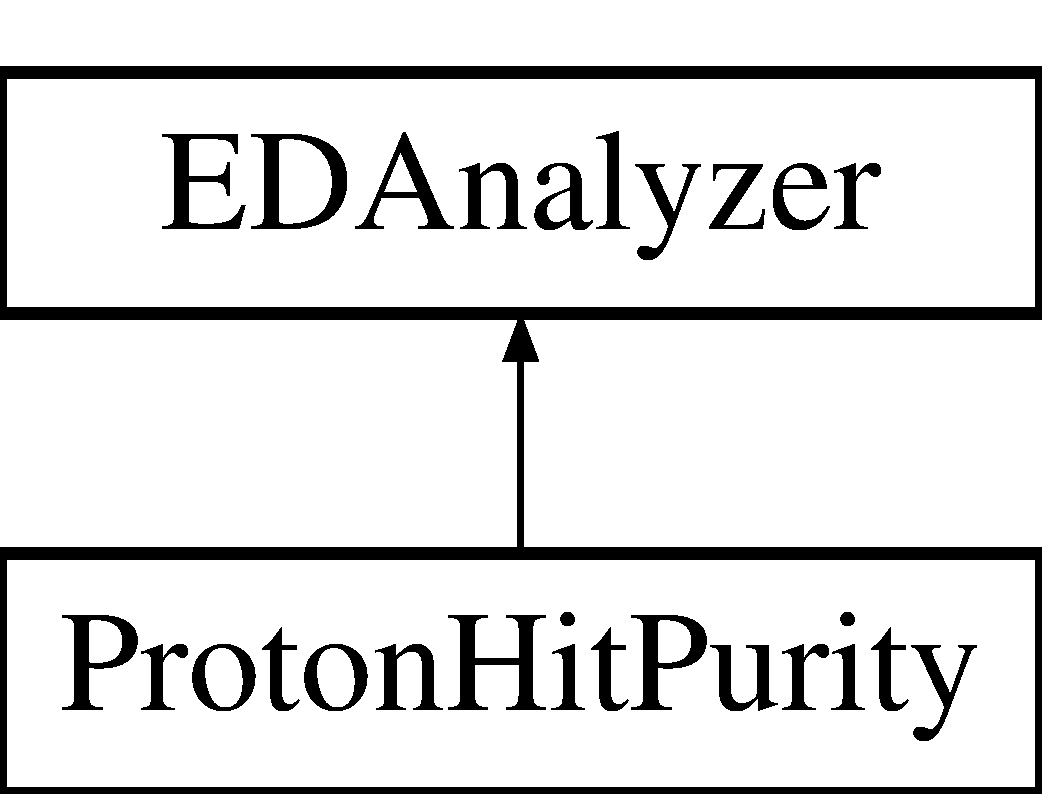
\includegraphics[height=2.000000cm]{classProtonHitPurity}
\end{center}
\end{figure}
\subsection*{Public Member Functions}
\begin{DoxyCompactItemize}
\item 
{\bfseries Proton\+Hit\+Purity} (fhicl\+::\+Parameter\+Set const \&p)\hypertarget{classProtonHitPurity_abe7eb14746a7e1555142a2f97dd6c8a7}{}\label{classProtonHitPurity_abe7eb14746a7e1555142a2f97dd6c8a7}

\item 
{\bfseries Proton\+Hit\+Purity} (\hyperlink{classProtonHitPurity}{Proton\+Hit\+Purity} const \&)=delete\hypertarget{classProtonHitPurity_a30e40f4da9dd297a45af8453698365be}{}\label{classProtonHitPurity_a30e40f4da9dd297a45af8453698365be}

\item 
{\bfseries Proton\+Hit\+Purity} (\hyperlink{classProtonHitPurity}{Proton\+Hit\+Purity} \&\&)=delete\hypertarget{classProtonHitPurity_a5893503a8818f9e2b060529ff01c5643}{}\label{classProtonHitPurity_a5893503a8818f9e2b060529ff01c5643}

\item 
\hyperlink{classProtonHitPurity}{Proton\+Hit\+Purity} \& {\bfseries operator=} (\hyperlink{classProtonHitPurity}{Proton\+Hit\+Purity} const \&)=delete\hypertarget{classProtonHitPurity_a79ea93f2e5ee376569b3db012f90bf72}{}\label{classProtonHitPurity_a79ea93f2e5ee376569b3db012f90bf72}

\item 
\hyperlink{classProtonHitPurity}{Proton\+Hit\+Purity} \& {\bfseries operator=} (\hyperlink{classProtonHitPurity}{Proton\+Hit\+Purity} \&\&)=delete\hypertarget{classProtonHitPurity_af5c3fb096ec529ada9dbdb69ce78053f}{}\label{classProtonHitPurity_af5c3fb096ec529ada9dbdb69ce78053f}

\item 
void {\bfseries analyze} (art\+::\+Event const \&e) override\hypertarget{classProtonHitPurity_a39595f8fc8677b6b95ce467f685ee276}{}\label{classProtonHitPurity_a39595f8fc8677b6b95ce467f685ee276}

\item 
void {\bfseries begin\+Job} () override\hypertarget{classProtonHitPurity_a6838668a5d854bd257375d1a437278ee}{}\label{classProtonHitPurity_a6838668a5d854bd257375d1a437278ee}

\item 
void {\bfseries end\+Job} () override\hypertarget{classProtonHitPurity_accac7c769c035cb43c9d6e5a780ab241}{}\label{classProtonHitPurity_accac7c769c035cb43c9d6e5a780ab241}

\end{DoxyCompactItemize}
\subsection*{Private Member Functions}
\begin{DoxyCompactItemize}
\item 
void \hyperlink{classProtonHitPurity_adfed832259669bb323f5a6a4eae7107e}{Build\+P\+F\+P\+Map} (const searchingfornues\+::\+Proxy\+Pfp\+Coll\+\_\+t \&pfp\+\_\+pxy\+\_\+col)
\begin{DoxyCompactList}\small\item\em function to builf a map linking P\+F\+Particle index to Self() attribute \end{DoxyCompactList}\item 
void \hyperlink{classProtonHitPurity_a7e468a256d51c80933e9bb9b6be77b94}{Add\+Daughters} (const searchingfornues\+::\+Proxy\+Pfp\+Elem\+\_\+t \&pfp\+\_\+pxy, const searchingfornues\+::\+Proxy\+Pfp\+Coll\+\_\+t \&pfp\+\_\+pxy\+\_\+col, std\+::vector$<$ searchingfornues\+::\+Proxy\+Pfp\+Elem\+\_\+t $>$ \&slice\+\_\+v)
\begin{DoxyCompactList}\small\item\em build P\+F\+Particle hierarchy (i.\+e. slice) from parent \mbox{[}recursive function\mbox{]} \end{DoxyCompactList}\item 
std\+::vector$<$ art\+::\+Ptr$<$ recob\+::\+Hit $>$ $>$ {\bfseries get\+Gauss\+Hits} (const std\+::vector$<$ art\+::\+Ptr$<$ recob\+::\+Hit $>$$>$ \&hits, const art\+::\+Valid\+Handle$<$ std\+::vector$<$ recob\+::\+Hit $>$ $>$ gaushit\+\_\+h)\hypertarget{classProtonHitPurity_af073c27c1dd243faec1019466e52dfdd}{}\label{classProtonHitPurity_af073c27c1dd243faec1019466e52dfdd}

\item 
bool {\bfseries Is\+Proton\+Isolated} (const std\+::vector$<$ art\+::\+Ptr$<$ recob\+::\+Hit $>$$>$ \&hits, const art\+::\+Valid\+Handle$<$ std\+::vector$<$ recob\+::\+Hit $>$ $>$ gaushit\+\_\+h)\hypertarget{classProtonHitPurity_a8738628194b94c23f7666d3c85170a27}{}\label{classProtonHitPurity_a8738628194b94c23f7666d3c85170a27}

\item 
void {\bfseries Proton\+Dot} (const float \&proton\+Wire, const float \&proton\+Time, const int \&pl, const T\+Vector3 \&shower\+Vtx, const T\+Vector3 \&shower\+Dir, float \&dot, float \&d2d)\hypertarget{classProtonHitPurity_a4b71c7c7e85e49f74bc98960166d1fcc}{}\label{classProtonHitPurity_a4b71c7c7e85e49f74bc98960166d1fcc}

\end{DoxyCompactItemize}
\subsection*{Private Attributes}
\begin{DoxyCompactItemize}
\item 
art\+::\+Input\+Tag {\bfseries f\+Clusterproducer}\hypertarget{classProtonHitPurity_a9cde3bb38128414175bdec828c258628}{}\label{classProtonHitPurity_a9cde3bb38128414175bdec828c258628}

\item 
art\+::\+Input\+Tag {\bfseries f\+H\+Tproducer}\hypertarget{classProtonHitPurity_a67a39931d4884a9b8551d5158f37c954}{}\label{classProtonHitPurity_a67a39931d4884a9b8551d5158f37c954}

\item 
art\+::\+Input\+Tag {\bfseries f\+Hitproducer}\hypertarget{classProtonHitPurity_a7285b631733a327b17852217edcf130c}{}\label{classProtonHitPurity_a7285b631733a327b17852217edcf130c}

\item 
art\+::\+Input\+Tag {\bfseries f\+M\+C\+Pproducer}\hypertarget{classProtonHitPurity_a582ca83452036a5a15bde53595858dab}{}\label{classProtonHitPurity_a582ca83452036a5a15bde53595858dab}

\item 
art\+::\+Input\+Tag {\bfseries f\+P\+F\+Pproducer}\hypertarget{classProtonHitPurity_a58af404af2943b95545b5435f984b34c}{}\label{classProtonHitPurity_a58af404af2943b95545b5435f984b34c}

\item 
art\+::\+Input\+Tag {\bfseries f\+S\+H\+Rproducer}\hypertarget{classProtonHitPurity_ae02e24d9473737eba23b266383f240b0}{}\label{classProtonHitPurity_ae02e24d9473737eba23b266383f240b0}

\item 
std\+::map$<$ unsigned int, unsigned int $>$ {\bfseries \+\_\+pfpmap}\hypertarget{classProtonHitPurity_abaa0fd0f88cca733f6e1f58248d22e9b}{}\label{classProtonHitPurity_abaa0fd0f88cca733f6e1f58248d22e9b}

\item 
float {\bfseries \+\_\+wire2cm}\hypertarget{classProtonHitPurity_a6dd665c27aa4b6da7b90127e1fb2d773}{}\label{classProtonHitPurity_a6dd665c27aa4b6da7b90127e1fb2d773}

\item 
float {\bfseries \+\_\+time2cm}\hypertarget{classProtonHitPurity_a8c08fb55f794adf3214370e803bb5a00}{}\label{classProtonHitPurity_a8c08fb55f794adf3214370e803bb5a00}

\item 
T\+Tree $\ast$ {\bfseries \+\_\+tree}\hypertarget{classProtonHitPurity_a099b95a1f761865698b3518566f161d7}{}\label{classProtonHitPurity_a099b95a1f761865698b3518566f161d7}

\item 
int {\bfseries \+\_\+nhit}\hypertarget{classProtonHitPurity_a6844c4cad1d4dde899d327788ffb1fbe}{}\label{classProtonHitPurity_a6844c4cad1d4dde899d327788ffb1fbe}

\item 
int {\bfseries \+\_\+plane}\hypertarget{classProtonHitPurity_aaa0874bba49cd73ac89fe3453f5e64d1}{}\label{classProtonHitPurity_aaa0874bba49cd73ac89fe3453f5e64d1}

\item 
float {\bfseries \+\_\+charge}\hypertarget{classProtonHitPurity_a517cc8f0dfc9a9a0ad5d9fc93df7c20d}{}\label{classProtonHitPurity_a517cc8f0dfc9a9a0ad5d9fc93df7c20d}

\item 
float {\bfseries \+\_\+purity}\hypertarget{classProtonHitPurity_a189e155a01fe3e39248465acddc04a8c}{}\label{classProtonHitPurity_a189e155a01fe3e39248465acddc04a8c}

\item 
float {\bfseries \+\_\+shrdot}\hypertarget{classProtonHitPurity_af81a5c842b98e216cc147e6df4b89946}{}\label{classProtonHitPurity_af81a5c842b98e216cc147e6df4b89946}

\item 
float {\bfseries \+\_\+shrdist}\hypertarget{classProtonHitPurity_ac45672d1231ae74ac9ffa9d5f7872de2}{}\label{classProtonHitPurity_ac45672d1231ae74ac9ffa9d5f7872de2}

\item 
float {\bfseries \+\_\+shrenergy}\hypertarget{classProtonHitPurity_a4a83bd7758deeddbc8356ceb61e1ba7f}{}\label{classProtonHitPurity_a4a83bd7758deeddbc8356ceb61e1ba7f}

\item 
int {\bfseries \+\_\+nshr}\hypertarget{classProtonHitPurity_aee140d918772b3317099286660d08f1e}{}\label{classProtonHitPurity_aee140d918772b3317099286660d08f1e}

\end{DoxyCompactItemize}


\subsection{Member Function Documentation}
\index{Proton\+Hit\+Purity@{Proton\+Hit\+Purity}!Add\+Daughters@{Add\+Daughters}}
\index{Add\+Daughters@{Add\+Daughters}!Proton\+Hit\+Purity@{Proton\+Hit\+Purity}}
\subsubsection[{\texorpdfstring{Add\+Daughters(const searchingfornues\+::\+Proxy\+Pfp\+Elem\+\_\+t \&pfp\+\_\+pxy, const searchingfornues\+::\+Proxy\+Pfp\+Coll\+\_\+t \&pfp\+\_\+pxy\+\_\+col, std\+::vector$<$ searchingfornues\+::\+Proxy\+Pfp\+Elem\+\_\+t $>$ \&slice\+\_\+v)}{AddDaughters(const searchingfornues::ProxyPfpElem_t &pfp_pxy, const searchingfornues::ProxyPfpColl_t &pfp_pxy_col, std::vector< searchingfornues::ProxyPfpElem_t > &slice_v)}}]{\setlength{\rightskip}{0pt plus 5cm}void Proton\+Hit\+Purity\+::\+Add\+Daughters (
\begin{DoxyParamCaption}
\item[{const searchingfornues\+::\+Proxy\+Pfp\+Elem\+\_\+t \&}]{pfp\+\_\+pxy, }
\item[{const searchingfornues\+::\+Proxy\+Pfp\+Coll\+\_\+t \&}]{pfp\+\_\+pxy\+\_\+col, }
\item[{std\+::vector$<$ searchingfornues\+::\+Proxy\+Pfp\+Elem\+\_\+t $>$ \&}]{slice\+\_\+v}
\end{DoxyParamCaption}
)\hspace{0.3cm}{\ttfamily [private]}}\hypertarget{classProtonHitPurity_a7e468a256d51c80933e9bb9b6be77b94}{}\label{classProtonHitPurity_a7e468a256d51c80933e9bb9b6be77b94}


build P\+F\+Particle hierarchy (i.\+e. slice) from parent \mbox{[}recursive function\mbox{]} 

pfp\+\_\+pxy \+: parent pfparticle proxy for which to add daughters  pfp\+\_\+pxy\+\_\+col \+: evnt P\+FP proxy collection  slice\+\_\+v \+: passed by reference, slice containing all P\+F\+Particles in hierarchy \index{Proton\+Hit\+Purity@{Proton\+Hit\+Purity}!Build\+P\+F\+P\+Map@{Build\+P\+F\+P\+Map}}
\index{Build\+P\+F\+P\+Map@{Build\+P\+F\+P\+Map}!Proton\+Hit\+Purity@{Proton\+Hit\+Purity}}
\subsubsection[{\texorpdfstring{Build\+P\+F\+P\+Map(const searchingfornues\+::\+Proxy\+Pfp\+Coll\+\_\+t \&pfp\+\_\+pxy\+\_\+col)}{BuildPFPMap(const searchingfornues::ProxyPfpColl_t &pfp_pxy_col)}}]{\setlength{\rightskip}{0pt plus 5cm}void Proton\+Hit\+Purity\+::\+Build\+P\+F\+P\+Map (
\begin{DoxyParamCaption}
\item[{const searchingfornues\+::\+Proxy\+Pfp\+Coll\+\_\+t \&}]{pfp\+\_\+pxy\+\_\+col}
\end{DoxyParamCaption}
)\hspace{0.3cm}{\ttfamily [private]}}\hypertarget{classProtonHitPurity_adfed832259669bb323f5a6a4eae7107e}{}\label{classProtonHitPurity_adfed832259669bb323f5a6a4eae7107e}


function to builf a map linking P\+F\+Particle index to Self() attribute 

handle to event pfparticle record 

The documentation for this class was generated from the following file\+:\begin{DoxyCompactItemize}
\item 
/home/travis/build/ubneutrinos/searchingfornues/\+Shower\+Reco/Proton\+Hit\+Purity\+\_\+module.\+cc\end{DoxyCompactItemize}

\hypertarget{classSaveSliceHits}{\section{Save\-Slice\-Hits Class Reference}
\label{classSaveSliceHits}\index{Save\-Slice\-Hits@{Save\-Slice\-Hits}}
}
Inheritance diagram for Save\-Slice\-Hits\-:\begin{figure}[H]
\begin{center}
\leavevmode
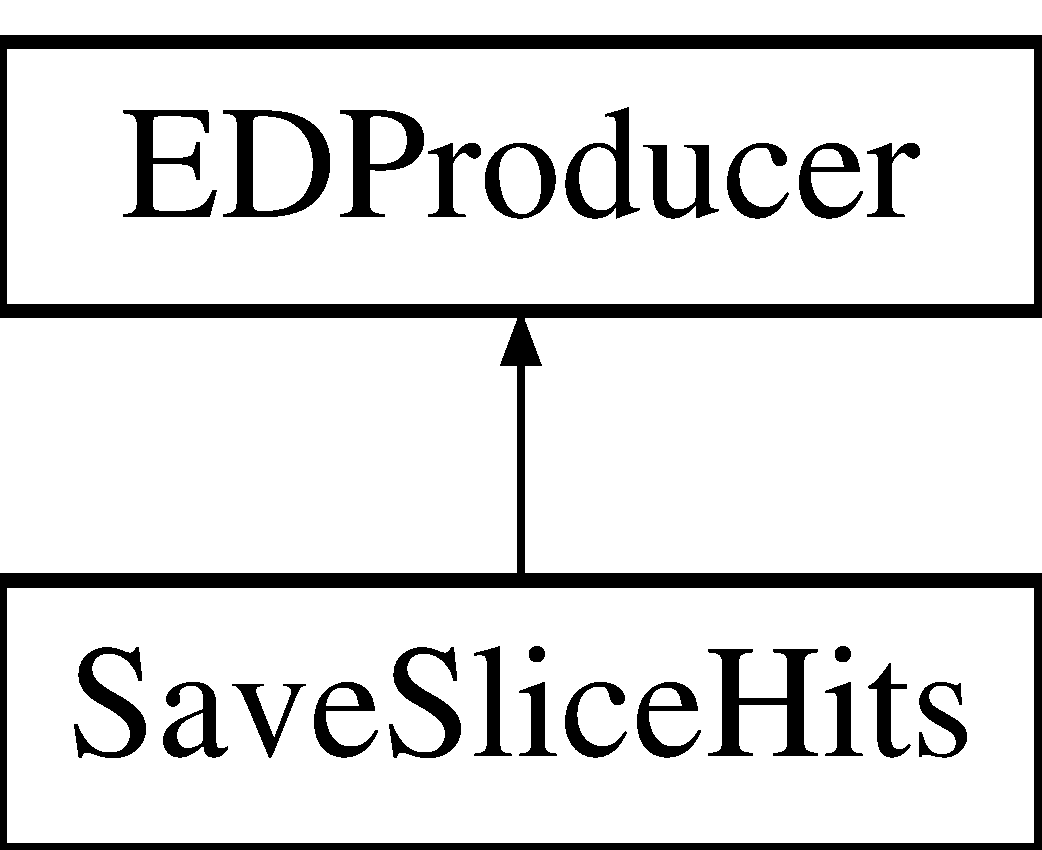
\includegraphics[height=2.000000cm]{classSaveSliceHits}
\end{center}
\end{figure}
\subsection*{Public Member Functions}
\begin{DoxyCompactItemize}
\item 
\hypertarget{classSaveSliceHits_a56e7e4878a9c004791e1d5a1c0555cd2}{{\bfseries Save\-Slice\-Hits} (fhicl\-::\-Parameter\-Set const \&p)}\label{classSaveSliceHits_a56e7e4878a9c004791e1d5a1c0555cd2}

\item 
\hypertarget{classSaveSliceHits_a21f4a1e618ae4562dd6aa2612f06849b}{{\bfseries Save\-Slice\-Hits} (\hyperlink{classSaveSliceHits}{Save\-Slice\-Hits} const \&)=delete}\label{classSaveSliceHits_a21f4a1e618ae4562dd6aa2612f06849b}

\item 
\hypertarget{classSaveSliceHits_a277a656266a5bfdac6491f0a59b8e441}{{\bfseries Save\-Slice\-Hits} (\hyperlink{classSaveSliceHits}{Save\-Slice\-Hits} \&\&)=delete}\label{classSaveSliceHits_a277a656266a5bfdac6491f0a59b8e441}

\item 
\hypertarget{classSaveSliceHits_ab30b09c8d4e1e79dfb9f105f412c90a1}{\hyperlink{classSaveSliceHits}{Save\-Slice\-Hits} \& {\bfseries operator=} (\hyperlink{classSaveSliceHits}{Save\-Slice\-Hits} const \&)=delete}\label{classSaveSliceHits_ab30b09c8d4e1e79dfb9f105f412c90a1}

\item 
\hypertarget{classSaveSliceHits_ae5329e70a6f07aef0b9a958a6abd0560}{\hyperlink{classSaveSliceHits}{Save\-Slice\-Hits} \& {\bfseries operator=} (\hyperlink{classSaveSliceHits}{Save\-Slice\-Hits} \&\&)=delete}\label{classSaveSliceHits_ae5329e70a6f07aef0b9a958a6abd0560}

\item 
\hypertarget{classSaveSliceHits_abec4f170d648b1855d5f26b563148cf6}{void {\bfseries produce} (art\-::\-Event \&e) override}\label{classSaveSliceHits_abec4f170d648b1855d5f26b563148cf6}

\item 
\hypertarget{classSaveSliceHits_a0ebe38a8c4f48a1d9c405787d076635a}{void {\bfseries begin\-Job} () override}\label{classSaveSliceHits_a0ebe38a8c4f48a1d9c405787d076635a}

\item 
\hypertarget{classSaveSliceHits_a48f6a563a927b9ff37d3a6f07462d8fd}{void {\bfseries end\-Job} () override}\label{classSaveSliceHits_a48f6a563a927b9ff37d3a6f07462d8fd}

\end{DoxyCompactItemize}
\subsection*{Private Member Functions}
\begin{DoxyCompactItemize}
\item 
\hypertarget{classSaveSliceHits_a13bfe5d175be84fe7b949a967a5da465}{void {\bfseries add\-Daughter} (const recob\-::\-P\-F\-Particle pfp, art\-::\-Valid\-Handle$<$ std\-::vector$<$ recob\-::\-P\-F\-Particle $>$ $>$ pfp\-\_\-h, art\-::\-Find\-Many\-P$<$ recob\-::\-Cluster $>$ pfp\-\_\-clus\-\_\-assn\-\_\-v, art\-::\-Find\-Many\-P$<$ recob\-::\-Hit $>$ clus\-\_\-hit\-\_\-assn\-\_\-v, std\-::vector$<$ unsigned int $>$ \&Pfp\-Hit\-Idx\-\_\-v)}\label{classSaveSliceHits_a13bfe5d175be84fe7b949a967a5da465}

\end{DoxyCompactItemize}
\subsection*{Private Attributes}
\begin{DoxyCompactItemize}
\item 
\hypertarget{classSaveSliceHits_a4a8537787643bd309b910620bcb2e154}{std\-::map$<$ unsigned int, \\*
unsigned int $>$ {\bfseries \-\_\-pfpmap}}\label{classSaveSliceHits_a4a8537787643bd309b910620bcb2e154}

\item 
\hypertarget{classSaveSliceHits_a6a289d782481d17dc39c931d62d0f31c}{art\-::\-Input\-Tag {\bfseries f\-Hitproducer}}\label{classSaveSliceHits_a6a289d782481d17dc39c931d62d0f31c}

\item 
\hypertarget{classSaveSliceHits_a4e6d5a3f1ab4ddc732f5758a3759effa}{art\-::\-Input\-Tag {\bfseries f\-Clusterproducer}}\label{classSaveSliceHits_a4e6d5a3f1ab4ddc732f5758a3759effa}

\item 
\hypertarget{classSaveSliceHits_ac2f381959f9bc912590888c6a86c8965}{art\-::\-Input\-Tag {\bfseries f\-Pfpproducer}}\label{classSaveSliceHits_ac2f381959f9bc912590888c6a86c8965}

\item 
\hypertarget{classSaveSliceHits_a942b1c4ea132e951aa39637e2f5d3e21}{art\-::\-Input\-Tag {\bfseries f\-Sliceproducer}}\label{classSaveSliceHits_a942b1c4ea132e951aa39637e2f5d3e21}

\item 
\hypertarget{classSaveSliceHits_a68cfd0c337276c49f781fa06495effb1}{float {\bfseries f\-Min\-Hit\-Charge}}\label{classSaveSliceHits_a68cfd0c337276c49f781fa06495effb1}

\end{DoxyCompactItemize}


The documentation for this class was generated from the following file\-:\begin{DoxyCompactItemize}
\item 
/home/travis/build/ubneutrinos/searchingfornues/\-Shower\-Reco/Save\-Slice\-Hits\-\_\-module.\-cc\end{DoxyCompactItemize}

\hypertarget{classSecondShowerPurity}{\section{Second\-Shower\-Purity Class Reference}
\label{classSecondShowerPurity}\index{Second\-Shower\-Purity@{Second\-Shower\-Purity}}
}
Inheritance diagram for Second\-Shower\-Purity\-:\begin{figure}[H]
\begin{center}
\leavevmode
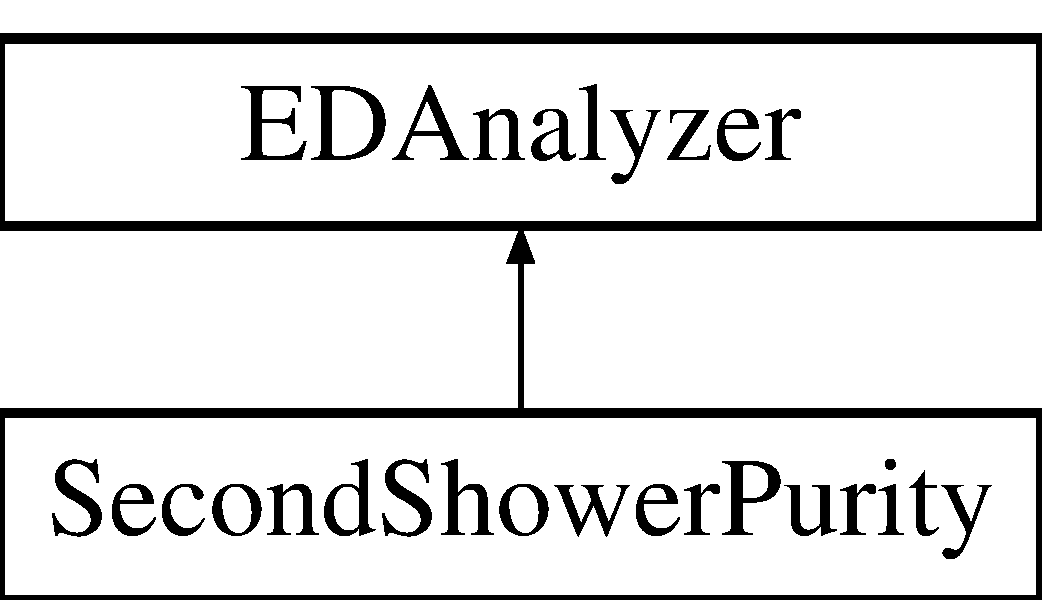
\includegraphics[height=2.000000cm]{classSecondShowerPurity}
\end{center}
\end{figure}
\subsection*{Public Member Functions}
\begin{DoxyCompactItemize}
\item 
\hypertarget{classSecondShowerPurity_a71eca6026bbad15c88a48b34137c3c9a}{{\bfseries Second\-Shower\-Purity} (fhicl\-::\-Parameter\-Set const \&p)}\label{classSecondShowerPurity_a71eca6026bbad15c88a48b34137c3c9a}

\item 
\hypertarget{classSecondShowerPurity_ac179e01d4ca5cc86bdbe60a96b7c77f6}{{\bfseries Second\-Shower\-Purity} (\hyperlink{classSecondShowerPurity}{Second\-Shower\-Purity} const \&)=delete}\label{classSecondShowerPurity_ac179e01d4ca5cc86bdbe60a96b7c77f6}

\item 
\hypertarget{classSecondShowerPurity_a84a772f635474b23f01ff0a9310a17ec}{{\bfseries Second\-Shower\-Purity} (\hyperlink{classSecondShowerPurity}{Second\-Shower\-Purity} \&\&)=delete}\label{classSecondShowerPurity_a84a772f635474b23f01ff0a9310a17ec}

\item 
\hypertarget{classSecondShowerPurity_a4eb7919d85a8756fe432dddd9061ea85}{\hyperlink{classSecondShowerPurity}{Second\-Shower\-Purity} \& {\bfseries operator=} (\hyperlink{classSecondShowerPurity}{Second\-Shower\-Purity} const \&)=delete}\label{classSecondShowerPurity_a4eb7919d85a8756fe432dddd9061ea85}

\item 
\hypertarget{classSecondShowerPurity_a6235a3f18b7a78b19a05047c644e31e4}{\hyperlink{classSecondShowerPurity}{Second\-Shower\-Purity} \& {\bfseries operator=} (\hyperlink{classSecondShowerPurity}{Second\-Shower\-Purity} \&\&)=delete}\label{classSecondShowerPurity_a6235a3f18b7a78b19a05047c644e31e4}

\item 
\hypertarget{classSecondShowerPurity_a3850d9497262ed256e5a7476d3982725}{void {\bfseries analyze} (art\-::\-Event const \&e) override}\label{classSecondShowerPurity_a3850d9497262ed256e5a7476d3982725}

\item 
\hypertarget{classSecondShowerPurity_a452d497e9edfaa2576a3b5a0540a22a8}{void {\bfseries begin\-Job} () override}\label{classSecondShowerPurity_a452d497e9edfaa2576a3b5a0540a22a8}

\item 
\hypertarget{classSecondShowerPurity_abf54dcc8e9113033b779484072ae1780}{void {\bfseries end\-Job} () override}\label{classSecondShowerPurity_abf54dcc8e9113033b779484072ae1780}

\end{DoxyCompactItemize}
\subsection*{Private Member Functions}
\begin{DoxyCompactItemize}
\item 
void \hyperlink{classSecondShowerPurity_a740e87a9a228f255bca15d2f04505aa9}{Build\-P\-F\-P\-Map} (const searchingfornues\-::\-Proxy\-Pfp\-Coll\-\_\-t \&pfp\-\_\-pxy\-\_\-col)
\begin{DoxyCompactList}\small\item\em function to builf a map linking P\-F\-Particle index to Self() attribute \end{DoxyCompactList}\item 
void \hyperlink{classSecondShowerPurity_a91a362195490bc158713e4ed84ed0fa2}{Add\-Daughters} (const searchingfornues\-::\-Proxy\-Pfp\-Elem\-\_\-t \&pfp\-\_\-pxy, const searchingfornues\-::\-Proxy\-Pfp\-Coll\-\_\-t \&pfp\-\_\-pxy\-\_\-col, std\-::vector$<$ searchingfornues\-::\-Proxy\-Pfp\-Elem\-\_\-t $>$ \&slice\-\_\-v)
\begin{DoxyCompactList}\small\item\em build P\-F\-Particle hierarchy (i.\-e. slice) from parent \mbox{[}recursive function\mbox{]} \end{DoxyCompactList}\item 
\hypertarget{classSecondShowerPurity_af58098493a2cd9014e1e962b366008e3}{void {\bfseries Reset\-T\-Tree} ()}\label{classSecondShowerPurity_af58098493a2cd9014e1e962b366008e3}

\item 
\hypertarget{classSecondShowerPurity_ad2c997fc6ccdea277c14cfcad5c83243}{std\-::vector$<$ art\-::\-Ptr\\*
$<$ recob\-::\-Hit $>$ $>$ {\bfseries get\-Gauss\-Hits} (const std\-::vector$<$ art\-::\-Ptr$<$ recob\-::\-Hit $>$$>$ \&hits, const art\-::\-Valid\-Handle$<$ std\-::vector$<$ recob\-::\-Hit $>$ $>$ gaushit\-\_\-h)}\label{classSecondShowerPurity_ad2c997fc6ccdea277c14cfcad5c83243}

\item 
\hypertarget{classSecondShowerPurity_aca45d8671bf9d292eed1ed00a80329b1}{bool {\bfseries Is\-Proton\-Isolated} (const std\-::vector$<$ art\-::\-Ptr$<$ recob\-::\-Hit $>$$>$ \&hits, const art\-::\-Valid\-Handle$<$ std\-::vector$<$ recob\-::\-Hit $>$ $>$ gaushit\-\_\-h)}\label{classSecondShowerPurity_aca45d8671bf9d292eed1ed00a80329b1}

\item 
\hypertarget{classSecondShowerPurity_ac3aa736b52623968b984814ac75d6510}{void {\bfseries Gamma\-Dot} (const float \&gamma\-Wire, const float \&gamma\-Time, const int \&pl, const T\-Vector3 \&shower\-Vtx, const T\-Vector3 \&shower\-Dir, float \&dot, float \&d2d)}\label{classSecondShowerPurity_ac3aa736b52623968b984814ac75d6510}

\item 
\hypertarget{classSecondShowerPurity_a57fd30974ec2f17538f54fbeaeb6f8ef}{void {\bfseries P\-C\-A} (const std\-::vector$<$ art\-::\-Ptr$<$ recob\-::\-Hit $>$$>$ \&hits, T\-Vector\-D \&eigen\-Val, T\-Matrix\-D \&eigen\-Vec)}\label{classSecondShowerPurity_a57fd30974ec2f17538f54fbeaeb6f8ef}

\item 
\hypertarget{classSecondShowerPurity_a7b112eddad9439ca96b2d25ce2e432b2}{float {\bfseries Eigen\-Dot} (const int \&pl, const T\-Vector3 \&Shower\-Dir, const float \&gamma\-Wire\-Dir, const float \&gamma\-Time\-Dir)}\label{classSecondShowerPurity_a7b112eddad9439ca96b2d25ce2e432b2}

\end{DoxyCompactItemize}
\subsection*{Private Attributes}
\begin{DoxyCompactItemize}
\item 
\hypertarget{classSecondShowerPurity_a641801003f7a8cab0bb13efc21583739}{art\-::\-Input\-Tag {\bfseries f\-Clusterproducer}}\label{classSecondShowerPurity_a641801003f7a8cab0bb13efc21583739}

\item 
\hypertarget{classSecondShowerPurity_aac4bc55cedfa1905dfb2c60197198007}{art\-::\-Input\-Tag {\bfseries f\-H\-Tproducer}}\label{classSecondShowerPurity_aac4bc55cedfa1905dfb2c60197198007}

\item 
\hypertarget{classSecondShowerPurity_a397ee926f1a3b5594fde75933b30b48b}{art\-::\-Input\-Tag {\bfseries f\-Hitproducer}}\label{classSecondShowerPurity_a397ee926f1a3b5594fde75933b30b48b}

\item 
\hypertarget{classSecondShowerPurity_ab3ba769b6c15e325813bad206a7a2223}{art\-::\-Input\-Tag {\bfseries f\-P\-F\-Pproducer}}\label{classSecondShowerPurity_ab3ba769b6c15e325813bad206a7a2223}

\item 
\hypertarget{classSecondShowerPurity_af3cade2862986deb0c2333f7a13208ea}{art\-::\-Input\-Tag {\bfseries f\-S\-H\-Rproducer}}\label{classSecondShowerPurity_af3cade2862986deb0c2333f7a13208ea}

\item 
\hypertarget{classSecondShowerPurity_a267de14095ad791afcca1f3f2a568a87}{art\-::\-Input\-Tag {\bfseries f\-M\-C\-Sproducer}}\label{classSecondShowerPurity_a267de14095ad791afcca1f3f2a568a87}

\item 
\hypertarget{classSecondShowerPurity_af8a380f40bb05c2cb9b63ed3cfd9aa0f}{std\-::map$<$ unsigned int, \\*
unsigned int $>$ {\bfseries \-\_\-pfpmap}}\label{classSecondShowerPurity_af8a380f40bb05c2cb9b63ed3cfd9aa0f}

\item 
\hypertarget{classSecondShowerPurity_a99010c0c89592e3dd9f696f490a1a7f7}{float {\bfseries \-\_\-wire2cm}}\label{classSecondShowerPurity_a99010c0c89592e3dd9f696f490a1a7f7}

\item 
\hypertarget{classSecondShowerPurity_ac3c7bec25a10542beb5f12e1f3fc03b2}{float {\bfseries \-\_\-time2cm}}\label{classSecondShowerPurity_ac3c7bec25a10542beb5f12e1f3fc03b2}

\item 
\hypertarget{classSecondShowerPurity_acc6a1cb74b439825c0c3e116e7e79990}{T\-Tree $\ast$ {\bfseries \-\_\-tree}}\label{classSecondShowerPurity_acc6a1cb74b439825c0c3e116e7e79990}

\item 
\hypertarget{classSecondShowerPurity_a66bab37a53c798be4b5bbb2fc3a83ef8}{int {\bfseries \-\_\-evt}}\label{classSecondShowerPurity_a66bab37a53c798be4b5bbb2fc3a83ef8}

\item 
\hypertarget{classSecondShowerPurity_ad88c2adccbe580a2b957745851b964f2}{int {\bfseries \-\_\-sub}}\label{classSecondShowerPurity_ad88c2adccbe580a2b957745851b964f2}

\item 
\hypertarget{classSecondShowerPurity_a50687a80fe0034dc68f142e0e3e4d2e7}{int {\bfseries \-\_\-run}}\label{classSecondShowerPurity_a50687a80fe0034dc68f142e0e3e4d2e7}

\item 
\hypertarget{classSecondShowerPurity_a4b4ced7189ab5da87a01efbf5efab94f}{int {\bfseries \-\_\-nhit}}\label{classSecondShowerPurity_a4b4ced7189ab5da87a01efbf5efab94f}

\item 
\hypertarget{classSecondShowerPurity_a46cb720b340572ad480511628fe77e89}{int {\bfseries \-\_\-plane}}\label{classSecondShowerPurity_a46cb720b340572ad480511628fe77e89}

\item 
\hypertarget{classSecondShowerPurity_a5bfedf045c3c104e60b2173ccb1d1338}{float {\bfseries \-\_\-charge}}\label{classSecondShowerPurity_a5bfedf045c3c104e60b2173ccb1d1338}

\item 
\hypertarget{classSecondShowerPurity_a96749b5f8597709f571d396df397c09e}{float {\bfseries \-\_\-purity}}\label{classSecondShowerPurity_a96749b5f8597709f571d396df397c09e}

\item 
\hypertarget{classSecondShowerPurity_ae0a9cfb0ee82ebce26388ad7178daf9f}{float {\bfseries \-\_\-shrpurity}}\label{classSecondShowerPurity_ae0a9cfb0ee82ebce26388ad7178daf9f}

\item 
\hypertarget{classSecondShowerPurity_ac760b87c66bded961e5af29ea7cc3b64}{float {\bfseries \-\_\-shrdot}}\label{classSecondShowerPurity_ac760b87c66bded961e5af29ea7cc3b64}

\item 
\hypertarget{classSecondShowerPurity_a5191904da66cd252ac24707a5bfdba35}{float {\bfseries \-\_\-shrdist}}\label{classSecondShowerPurity_a5191904da66cd252ac24707a5bfdba35}

\item 
\hypertarget{classSecondShowerPurity_ae3810da69d504451c1b672f28bac844d}{float {\bfseries \-\_\-shrenergy1}}\label{classSecondShowerPurity_ae3810da69d504451c1b672f28bac844d}

\item 
\hypertarget{classSecondShowerPurity_ac8bbe37eaab32aa01e3cc45a9e4c832f}{float {\bfseries \-\_\-shrenergy2}}\label{classSecondShowerPurity_ac8bbe37eaab32aa01e3cc45a9e4c832f}

\item 
\hypertarget{classSecondShowerPurity_ac0bbff3715b04519f7db91a629ef7c35}{float {\bfseries \-\_\-elecenergy}}\label{classSecondShowerPurity_ac0bbff3715b04519f7db91a629ef7c35}

\item 
\hypertarget{classSecondShowerPurity_a29675be4a26901ae658f9ffbd6889ae6}{int {\bfseries \-\_\-btpdg}}\label{classSecondShowerPurity_a29675be4a26901ae658f9ffbd6889ae6}

\item 
\hypertarget{classSecondShowerPurity_a8d015e44e5d31083168e8c05b52a4efb}{int {\bfseries \-\_\-btshrpdg}}\label{classSecondShowerPurity_a8d015e44e5d31083168e8c05b52a4efb}

\item 
\hypertarget{classSecondShowerPurity_a2bffd624cb6a4b222e2814fefa402dee}{float {\bfseries \-\_\-btmom}}\label{classSecondShowerPurity_a2bffd624cb6a4b222e2814fefa402dee}

\item 
\hypertarget{classSecondShowerPurity_aac1a23423e956381fbc91668b6581f8f}{float {\bfseries \-\_\-btshrmom}}\label{classSecondShowerPurity_aac1a23423e956381fbc91668b6581f8f}

\item 
\hypertarget{classSecondShowerPurity_a0031191dddf516922b44958d3b32d54c}{int {\bfseries \-\_\-nshr}}\label{classSecondShowerPurity_a0031191dddf516922b44958d3b32d54c}

\item 
\hypertarget{classSecondShowerPurity_afba07fb9b16751cef928d2d0073b4cb6}{float {\bfseries \-\_\-clus\-\_\-tmin}}\label{classSecondShowerPurity_afba07fb9b16751cef928d2d0073b4cb6}

\item 
\hypertarget{classSecondShowerPurity_a112db666388cf84b52bd6631f7d48ab7}{float {\bfseries \-\_\-clus\-\_\-tmax}}\label{classSecondShowerPurity_a112db666388cf84b52bd6631f7d48ab7}

\item 
\hypertarget{classSecondShowerPurity_ab3955e8709105007782b28b724532a1a}{float {\bfseries \-\_\-twoshrdot}}\label{classSecondShowerPurity_ab3955e8709105007782b28b724532a1a}

\item 
\hypertarget{classSecondShowerPurity_a1bfb77f818b351085cb7515077d24c6b}{float {\bfseries \-\_\-eigenratio}}\label{classSecondShowerPurity_a1bfb77f818b351085cb7515077d24c6b}

\item 
\hypertarget{classSecondShowerPurity_a9dde548cb4088f572c339ed1fef58c30}{float {\bfseries \-\_\-eigendot}}\label{classSecondShowerPurity_a9dde548cb4088f572c339ed1fef58c30}

\item 
\hypertarget{classSecondShowerPurity_a97588e6b26578179932a8f6023728dde}{float {\bfseries \-\_\-gammaemin}}\label{classSecondShowerPurity_a97588e6b26578179932a8f6023728dde}

\end{DoxyCompactItemize}


\subsection{Member Function Documentation}
\hypertarget{classSecondShowerPurity_a91a362195490bc158713e4ed84ed0fa2}{\index{Second\-Shower\-Purity@{Second\-Shower\-Purity}!Add\-Daughters@{Add\-Daughters}}
\index{Add\-Daughters@{Add\-Daughters}!SecondShowerPurity@{Second\-Shower\-Purity}}
\subsubsection[{Add\-Daughters}]{\setlength{\rightskip}{0pt plus 5cm}void Second\-Shower\-Purity\-::\-Add\-Daughters (
\begin{DoxyParamCaption}
\item[{const searchingfornues\-::\-Proxy\-Pfp\-Elem\-\_\-t \&}]{pfp\-\_\-pxy, }
\item[{const searchingfornues\-::\-Proxy\-Pfp\-Coll\-\_\-t \&}]{pfp\-\_\-pxy\-\_\-col, }
\item[{std\-::vector$<$ searchingfornues\-::\-Proxy\-Pfp\-Elem\-\_\-t $>$ \&}]{slice\-\_\-v}
\end{DoxyParamCaption}
)\hspace{0.3cm}{\ttfamily [private]}}}\label{classSecondShowerPurity_a91a362195490bc158713e4ed84ed0fa2}


build P\-F\-Particle hierarchy (i.\-e. slice) from parent \mbox{[}recursive function\mbox{]} 

pfp\-\_\-pxy \-: parent pfparticle proxy for which to add daughters  pfp\-\_\-pxy\-\_\-col \-: evnt P\-F\-P proxy collection  slice\-\_\-v \-: passed by reference, slice containing all P\-F\-Particles in hierarchy \hypertarget{classSecondShowerPurity_a740e87a9a228f255bca15d2f04505aa9}{\index{Second\-Shower\-Purity@{Second\-Shower\-Purity}!Build\-P\-F\-P\-Map@{Build\-P\-F\-P\-Map}}
\index{Build\-P\-F\-P\-Map@{Build\-P\-F\-P\-Map}!SecondShowerPurity@{Second\-Shower\-Purity}}
\subsubsection[{Build\-P\-F\-P\-Map}]{\setlength{\rightskip}{0pt plus 5cm}void Second\-Shower\-Purity\-::\-Build\-P\-F\-P\-Map (
\begin{DoxyParamCaption}
\item[{const searchingfornues\-::\-Proxy\-Pfp\-Coll\-\_\-t \&}]{pfp\-\_\-pxy\-\_\-col}
\end{DoxyParamCaption}
)\hspace{0.3cm}{\ttfamily [private]}}}\label{classSecondShowerPurity_a740e87a9a228f255bca15d2f04505aa9}


function to builf a map linking P\-F\-Particle index to Self() attribute 

handle to event pfparticle record 

The documentation for this class was generated from the following file\-:\begin{DoxyCompactItemize}
\item 
/home/travis/build/ubneutrinos/searchingfornues/\-Shower\-Reco/Second\-Shower\-Purity\-\_\-module.\-cc\end{DoxyCompactItemize}

\hypertarget{classselection_1_1SelectionExample}{}\section{selection\+:\+:Selection\+Example Class Reference}
\label{classselection_1_1SelectionExample}\index{selection\+::\+Selection\+Example@{selection\+::\+Selection\+Example}}
Inheritance diagram for selection\+:\+:Selection\+Example\+:\begin{figure}[H]
\begin{center}
\leavevmode
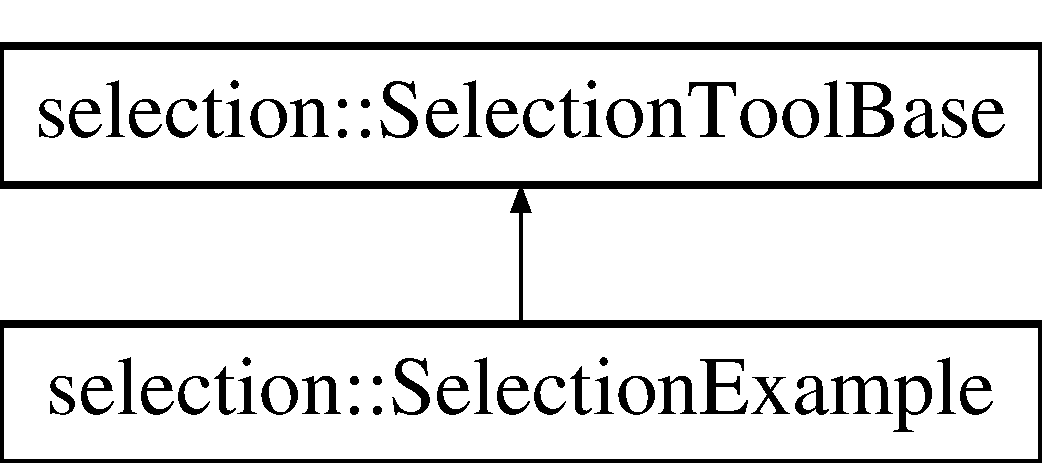
\includegraphics[height=2.000000cm]{classselection_1_1SelectionExample}
\end{center}
\end{figure}
\subsection*{Public Member Functions}
\begin{DoxyCompactItemize}
\item 
\hyperlink{classselection_1_1SelectionExample_a14d995ca3f3beda222bf5eb514fde63f}{Selection\+Example} (const fhicl\+::\+Parameter\+Set \&pset)
\begin{DoxyCompactList}\small\item\em Constructor. \end{DoxyCompactList}\item 
\hyperlink{classselection_1_1SelectionExample_a23080e1af959ccac8b922ebae7dd1d73}{$\sim$\+Selection\+Example} ()\hypertarget{classselection_1_1SelectionExample_a23080e1af959ccac8b922ebae7dd1d73}{}\label{classselection_1_1SelectionExample_a23080e1af959ccac8b922ebae7dd1d73}

\begin{DoxyCompactList}\small\item\em Destructor. \end{DoxyCompactList}\item 
void \hyperlink{classselection_1_1SelectionExample_a93e07083284b112e1881aca28a4205aa}{configure} (fhicl\+::\+Parameter\+Set const \&pset)
\item 
bool \hyperlink{classselection_1_1SelectionExample_a25a0971c86e5b6fb2ce51c16c0a58f9e}{select\+Event} (art\+::\+Event const \&e, const std\+::vector$<$ Proxy\+Pfp\+Elem\+\_\+t $>$ \&pfp\+\_\+pxy\+\_\+v)
\begin{DoxyCompactList}\small\item\em Selection function. \end{DoxyCompactList}\item 
void \hyperlink{classselection_1_1SelectionExample_a6d40ae8dec191b9985338aed2047b1ec}{set\+Branches} (T\+Tree $\ast$\+\_\+tree)\hypertarget{classselection_1_1SelectionExample_a6d40ae8dec191b9985338aed2047b1ec}{}\label{classselection_1_1SelectionExample_a6d40ae8dec191b9985338aed2047b1ec}

\begin{DoxyCompactList}\small\item\em set branches for T\+Tree \end{DoxyCompactList}\item 
void \hyperlink{classselection_1_1SelectionExample_aeca20c0b0258d6a31bf563a9c9728595}{reset\+T\+Tree} (T\+Tree $\ast$\+\_\+tree)\hypertarget{classselection_1_1SelectionExample_aeca20c0b0258d6a31bf563a9c9728595}{}\label{classselection_1_1SelectionExample_aeca20c0b0258d6a31bf563a9c9728595}

\begin{DoxyCompactList}\small\item\em reset ttree branches \end{DoxyCompactList}\end{DoxyCompactItemize}
\subsection*{Private Attributes}
\begin{DoxyCompactItemize}
\item 
unsigned int {\bfseries \+\_\+multiplicity}\hypertarget{classselection_1_1SelectionExample_aa489e0107cecbb9a039dc3fb52c728f1}{}\label{classselection_1_1SelectionExample_aa489e0107cecbb9a039dc3fb52c728f1}

\end{DoxyCompactItemize}
\subsection*{Additional Inherited Members}


\subsection{Constructor \& Destructor Documentation}
\index{selection\+::\+Selection\+Example@{selection\+::\+Selection\+Example}!Selection\+Example@{Selection\+Example}}
\index{Selection\+Example@{Selection\+Example}!selection\+::\+Selection\+Example@{selection\+::\+Selection\+Example}}
\subsubsection[{\texorpdfstring{Selection\+Example(const fhicl\+::\+Parameter\+Set \&pset)}{SelectionExample(const fhicl::ParameterSet &pset)}}]{\setlength{\rightskip}{0pt plus 5cm}selection\+::\+Selection\+Example\+::\+Selection\+Example (
\begin{DoxyParamCaption}
\item[{const fhicl\+::\+Parameter\+Set \&}]{pset}
\end{DoxyParamCaption}
)}\hypertarget{classselection_1_1SelectionExample_a14d995ca3f3beda222bf5eb514fde63f}{}\label{classselection_1_1SelectionExample_a14d995ca3f3beda222bf5eb514fde63f}


Constructor. 


\begin{DoxyParams}{Parameters}
{\em pset} & Constructor.\\
\hline
\end{DoxyParams}
Arguments\+:

pset -\/ Fcl parameters. 

\subsection{Member Function Documentation}
\index{selection\+::\+Selection\+Example@{selection\+::\+Selection\+Example}!configure@{configure}}
\index{configure@{configure}!selection\+::\+Selection\+Example@{selection\+::\+Selection\+Example}}
\subsubsection[{\texorpdfstring{configure(fhicl\+::\+Parameter\+Set const \&pset)}{configure(fhicl::ParameterSet const &pset)}}]{\setlength{\rightskip}{0pt plus 5cm}void selection\+::\+Selection\+Example\+::configure (
\begin{DoxyParamCaption}
\item[{fhicl\+::\+Parameter\+Set const \&}]{pset}
\end{DoxyParamCaption}
)}\hypertarget{classselection_1_1SelectionExample_a93e07083284b112e1881aca28a4205aa}{}\label{classselection_1_1SelectionExample_a93e07083284b112e1881aca28a4205aa}
Reconfigure method.

Arguments\+:

pset -\/ Fcl parameter set. \index{selection\+::\+Selection\+Example@{selection\+::\+Selection\+Example}!select\+Event@{select\+Event}}
\index{select\+Event@{select\+Event}!selection\+::\+Selection\+Example@{selection\+::\+Selection\+Example}}
\subsubsection[{\texorpdfstring{select\+Event(art\+::\+Event const \&e, const std\+::vector$<$ Proxy\+Pfp\+Elem\+\_\+t $>$ \&pfp\+\_\+pxy\+\_\+v)}{selectEvent(art::Event const &e, const std::vector< ProxyPfpElem_t > &pfp_pxy_v)}}]{\setlength{\rightskip}{0pt plus 5cm}bool selection\+::\+Selection\+Example\+::select\+Event (
\begin{DoxyParamCaption}
\item[{art\+::\+Event const \&}]{e, }
\item[{const std\+::vector$<$ Proxy\+Pfp\+Elem\+\_\+t $>$ \&}]{pfp\+\_\+pxy\+\_\+v}
\end{DoxyParamCaption}
)\hspace{0.3cm}{\ttfamily [virtual]}}\hypertarget{classselection_1_1SelectionExample_a25a0971c86e5b6fb2ce51c16c0a58f9e}{}\label{classselection_1_1SelectionExample_a25a0971c86e5b6fb2ce51c16c0a58f9e}


Selection function. 

Reconfigure method.

Arguments\+:

pset -\/ Fcl parameter set. 

Implements \hyperlink{classselection_1_1SelectionToolBase_ab63818dac49b43418fe9eb3b8cd98c9c}{selection\+::\+Selection\+Tool\+Base}.



The documentation for this class was generated from the following file\+:\begin{DoxyCompactItemize}
\item 
/home/travis/build/ubneutrinos/searchingfornues/\+Selection/\+Selection\+Tools/Selection\+Example\+\_\+tool.\+cc\end{DoxyCompactItemize}

\hypertarget{classselection_1_1SelectionToolBase}{\section{selection\-:\-:Selection\-Tool\-Base Class Reference}
\label{classselection_1_1SelectionToolBase}\index{selection\-::\-Selection\-Tool\-Base@{selection\-::\-Selection\-Tool\-Base}}
}
Inheritance diagram for selection\-:\-:Selection\-Tool\-Base\-:\begin{figure}[H]
\begin{center}
\leavevmode
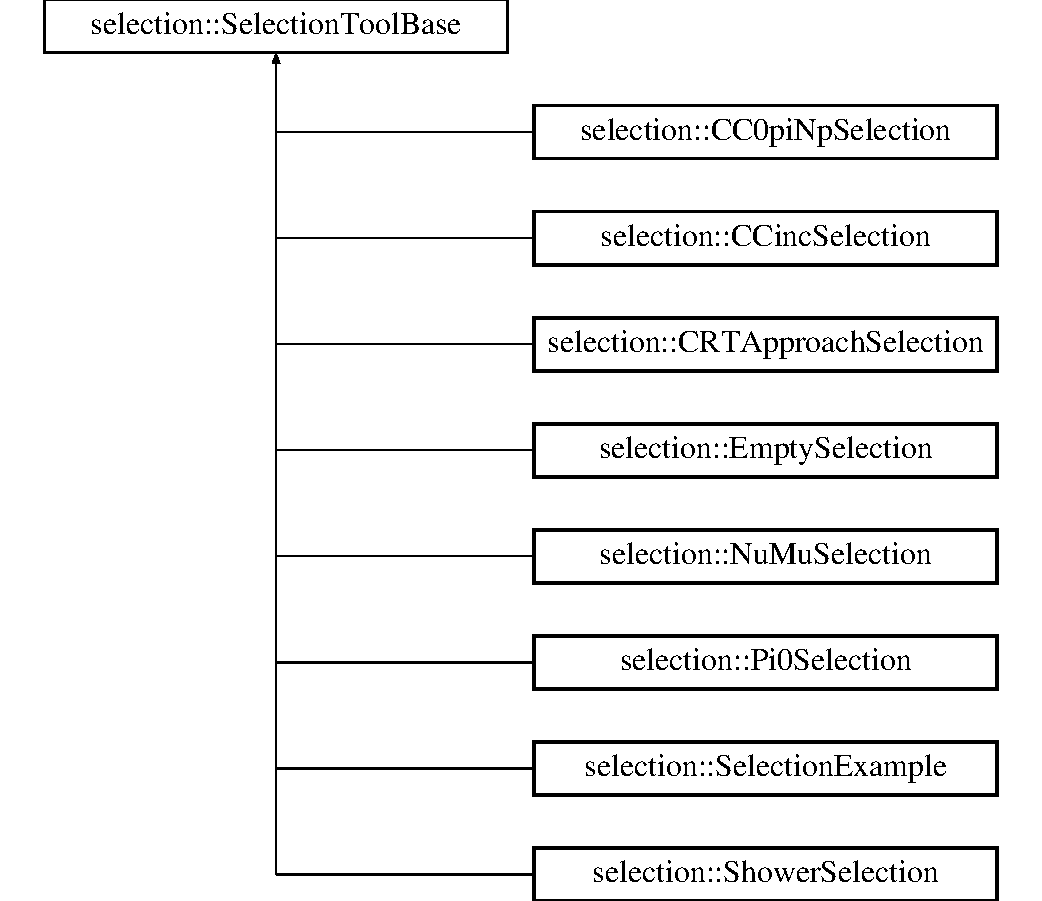
\includegraphics[height=9.000000cm]{classselection_1_1SelectionToolBase}
\end{center}
\end{figure}
\subsection*{Public Member Functions}
\begin{DoxyCompactItemize}
\item 
\hypertarget{classselection_1_1SelectionToolBase_a79885af9ff5ab77d239d8484c22ac87e}{virtual \hyperlink{classselection_1_1SelectionToolBase_a79885af9ff5ab77d239d8484c22ac87e}{$\sim$\-Selection\-Tool\-Base} () noexcept=default}\label{classselection_1_1SelectionToolBase_a79885af9ff5ab77d239d8484c22ac87e}

\begin{DoxyCompactList}\small\item\em Virtual Destructor. \end{DoxyCompactList}\item 
void \hyperlink{classselection_1_1SelectionToolBase_a36b68431bd5d3f815619d989faa7ef02}{configure} (const fhicl\-::\-Parameter\-Set \&)
\begin{DoxyCompactList}\small\item\em Interface for configuring the particular algorithm tool. \end{DoxyCompactList}\item 
virtual bool \hyperlink{classselection_1_1SelectionToolBase_ab63818dac49b43418fe9eb3b8cd98c9c}{select\-Event} (art\-::\-Event const \&e, const std\-::vector$<$ Proxy\-Pfp\-Elem\-\_\-t $>$ \&pfp\-\_\-pxy\-\_\-v)=0
\begin{DoxyCompactList}\small\item\em Selection function. \end{DoxyCompactList}\item 
\hypertarget{classselection_1_1SelectionToolBase_aa97ea5e55391240d8e251dae13897996}{virtual void \hyperlink{classselection_1_1SelectionToolBase_aa97ea5e55391240d8e251dae13897996}{set\-Branches} (T\-Tree $\ast$\-\_\-tree)=0}\label{classselection_1_1SelectionToolBase_aa97ea5e55391240d8e251dae13897996}

\begin{DoxyCompactList}\small\item\em set branches for T\-Tree \end{DoxyCompactList}\item 
\hypertarget{classselection_1_1SelectionToolBase_ae51d9c23ceee13bebf196d6535d5f1a5}{virtual void \hyperlink{classselection_1_1SelectionToolBase_ae51d9c23ceee13bebf196d6535d5f1a5}{reset\-T\-Tree} (T\-Tree $\ast$\-\_\-tree)=0}\label{classselection_1_1SelectionToolBase_ae51d9c23ceee13bebf196d6535d5f1a5}

\begin{DoxyCompactList}\small\item\em resetset T\-Tree branches \end{DoxyCompactList}\item 
\hypertarget{classselection_1_1SelectionToolBase_a92ab2f99d650c4a2628cd042a7d09711}{void \hyperlink{classselection_1_1SelectionToolBase_a92ab2f99d650c4a2628cd042a7d09711}{Set\-Data} (bool isdata)}\label{classselection_1_1SelectionToolBase_a92ab2f99d650c4a2628cd042a7d09711}

\begin{DoxyCompactList}\small\item\em set if data \end{DoxyCompactList}\end{DoxyCompactItemize}
\subsection*{Protected Attributes}
\begin{DoxyCompactItemize}
\item 
\hypertarget{classselection_1_1SelectionToolBase_a6de7e9c8fc22c23ee3c13f0b92cde326}{bool {\bfseries f\-Data}}\label{classselection_1_1SelectionToolBase_a6de7e9c8fc22c23ee3c13f0b92cde326}

\end{DoxyCompactItemize}


\subsection{Member Function Documentation}
\hypertarget{classselection_1_1SelectionToolBase_a36b68431bd5d3f815619d989faa7ef02}{\index{selection\-::\-Selection\-Tool\-Base@{selection\-::\-Selection\-Tool\-Base}!configure@{configure}}
\index{configure@{configure}!selection::SelectionToolBase@{selection\-::\-Selection\-Tool\-Base}}
\subsubsection[{configure}]{\setlength{\rightskip}{0pt plus 5cm}void selection\-::\-Selection\-Tool\-Base\-::configure (
\begin{DoxyParamCaption}
\item[{const fhicl\-::\-Parameter\-Set \&}]{}
\end{DoxyParamCaption}
)\hspace{0.3cm}{\ttfamily [inline]}}}\label{classselection_1_1SelectionToolBase_a36b68431bd5d3f815619d989faa7ef02}


Interface for configuring the particular algorithm tool. 


\begin{DoxyParams}{Parameters}
{\em Parameter\-Set} & The input set of parameters for configuration \\
\hline
\end{DoxyParams}
\hypertarget{classselection_1_1SelectionToolBase_ab63818dac49b43418fe9eb3b8cd98c9c}{\index{selection\-::\-Selection\-Tool\-Base@{selection\-::\-Selection\-Tool\-Base}!select\-Event@{select\-Event}}
\index{select\-Event@{select\-Event}!selection::SelectionToolBase@{selection\-::\-Selection\-Tool\-Base}}
\subsubsection[{select\-Event}]{\setlength{\rightskip}{0pt plus 5cm}virtual bool selection\-::\-Selection\-Tool\-Base\-::select\-Event (
\begin{DoxyParamCaption}
\item[{art\-::\-Event const \&}]{e, }
\item[{const std\-::vector$<$ Proxy\-Pfp\-Elem\-\_\-t $>$ \&}]{pfp\-\_\-pxy\-\_\-v}
\end{DoxyParamCaption}
)\hspace{0.3cm}{\ttfamily [pure virtual]}}}\label{classselection_1_1SelectionToolBase_ab63818dac49b43418fe9eb3b8cd98c9c}


Selection function. 


\begin{DoxyParams}{Parameters}
{\em art\-::\-Event} & event record for selection \\
\hline
\end{DoxyParams}


Implemented in \hyperlink{classselection_1_1CRTApproachSelection_a9dffc74d919ac0586d57c1de740f4ce9}{selection\-::\-C\-R\-T\-Approach\-Selection}, \hyperlink{classselection_1_1CC0piNpSelection_aee88d296a2ebad59acadfd919139d96f}{selection\-::\-C\-C0pi\-Np\-Selection}, \hyperlink{classselection_1_1NuMuSelection_ad9aaf5eedf311e33cb6e7f54e2605c98}{selection\-::\-Nu\-Mu\-Selection}, \hyperlink{classselection_1_1Pi0Selection_a1efba82b7ec3c2e18a48a98605720009}{selection\-::\-Pi0\-Selection}, \hyperlink{classselection_1_1ShowerSelection_aa538b905ab6e8a329acf3eaa97cc0af9}{selection\-::\-Shower\-Selection}, \hyperlink{classselection_1_1EmptySelection_a4ecce282e53d9d7c6c4764eef0b808f7}{selection\-::\-Empty\-Selection}, \hyperlink{classselection_1_1SelectionExample_a25a0971c86e5b6fb2ce51c16c0a58f9e}{selection\-::\-Selection\-Example}, and \hyperlink{classselection_1_1CCincSelection_ae8555674551f611dee06dc315ac2987f}{selection\-::\-C\-Cinc\-Selection}.



The documentation for this class was generated from the following file\-:\begin{DoxyCompactItemize}
\item 
/home/travis/build/ubneutrinos/searchingfornues/\-Selection/\-Selection\-Tools/Selection\-Tool\-Base.\-h\end{DoxyCompactItemize}

\hypertarget{classanalysis_1_1ShowerAnalysis}{}\section{analysis\+:\+:Shower\+Analysis Class Reference}
\label{classanalysis_1_1ShowerAnalysis}\index{analysis\+::\+Shower\+Analysis@{analysis\+::\+Shower\+Analysis}}
Inheritance diagram for analysis\+:\+:Shower\+Analysis\+:\begin{figure}[H]
\begin{center}
\leavevmode
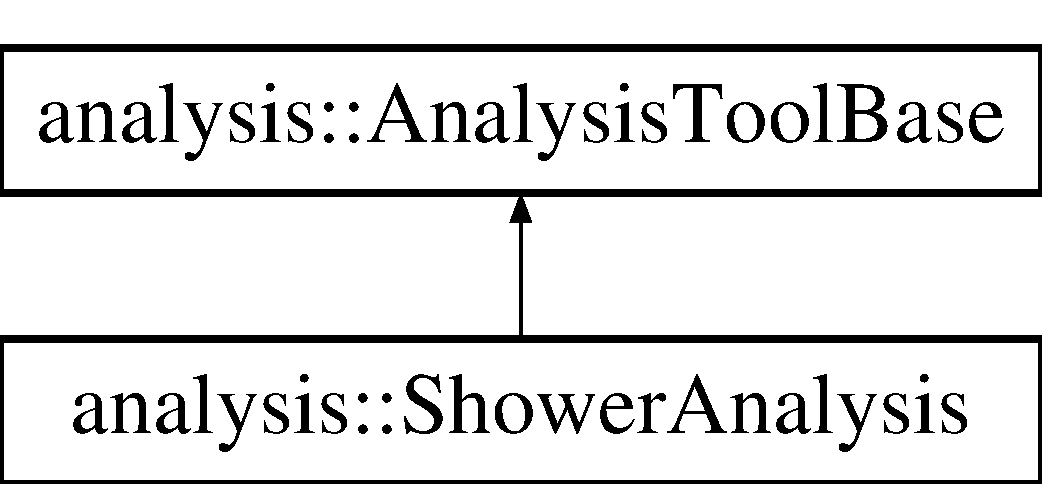
\includegraphics[height=2.000000cm]{classanalysis_1_1ShowerAnalysis}
\end{center}
\end{figure}
\subsection*{Public Member Functions}
\begin{DoxyCompactItemize}
\item 
\hyperlink{classanalysis_1_1ShowerAnalysis_a6ea40aa403312ba7acc5434c1c66df63}{Shower\+Analysis} (const fhicl\+::\+Parameter\+Set \&pset)
\begin{DoxyCompactList}\small\item\em Constructor. \end{DoxyCompactList}\item 
\hyperlink{classanalysis_1_1ShowerAnalysis_af16c1759f0122ba30f7839c4003c0df7}{$\sim$\+Shower\+Analysis} ()\hypertarget{classanalysis_1_1ShowerAnalysis_af16c1759f0122ba30f7839c4003c0df7}{}\label{classanalysis_1_1ShowerAnalysis_af16c1759f0122ba30f7839c4003c0df7}

\begin{DoxyCompactList}\small\item\em Destructor. \end{DoxyCompactList}\item 
void \hyperlink{classanalysis_1_1ShowerAnalysis_a973cb90e6fa423b88ca3a9667d467b1e}{configure} (fhicl\+::\+Parameter\+Set const \&pset)
\item 
void \hyperlink{classanalysis_1_1ShowerAnalysis_a5ae15109590ea737320bf13cefa5cc3f}{analyze\+Event} (art\+::\+Event const \&e, bool f\+Data) override
\begin{DoxyCompactList}\small\item\em Analysis function. \end{DoxyCompactList}\item 
void \hyperlink{classanalysis_1_1ShowerAnalysis_a957be06c08e5777cd684c84ca53bc45e}{analyze\+Slice} (art\+::\+Event const \&e, std\+::vector$<$ Proxy\+Pfp\+Elem\+\_\+t $>$ \&slice\+\_\+pfp\+\_\+v, bool f\+Data, bool selected) override\hypertarget{classanalysis_1_1ShowerAnalysis_a957be06c08e5777cd684c84ca53bc45e}{}\label{classanalysis_1_1ShowerAnalysis_a957be06c08e5777cd684c84ca53bc45e}

\begin{DoxyCompactList}\small\item\em Analyze slice. \end{DoxyCompactList}\item 
void \hyperlink{classanalysis_1_1ShowerAnalysis_a0753806916baaf34f1ab0efa0dc4f4cc}{Save\+Truth} (art\+::\+Event const \&e)\hypertarget{classanalysis_1_1ShowerAnalysis_a0753806916baaf34f1ab0efa0dc4f4cc}{}\label{classanalysis_1_1ShowerAnalysis_a0753806916baaf34f1ab0efa0dc4f4cc}

\begin{DoxyCompactList}\small\item\em Save truth info for event associated to neutrino. \end{DoxyCompactList}\item 
void \hyperlink{classanalysis_1_1ShowerAnalysis_aab587f04c820fa5ce9542715f396a1cf}{fill\+Default} ()\hypertarget{classanalysis_1_1ShowerAnalysis_aab587f04c820fa5ce9542715f396a1cf}{}\label{classanalysis_1_1ShowerAnalysis_aab587f04c820fa5ce9542715f396a1cf}

\begin{DoxyCompactList}\small\item\em Fill Default info for event associated to neutrino. \end{DoxyCompactList}\item 
void \hyperlink{classanalysis_1_1ShowerAnalysis_a007102f8d6c1f72551124b35b846662d}{set\+Branches} (T\+Tree $\ast$\+\_\+tree) override\hypertarget{classanalysis_1_1ShowerAnalysis_a007102f8d6c1f72551124b35b846662d}{}\label{classanalysis_1_1ShowerAnalysis_a007102f8d6c1f72551124b35b846662d}

\begin{DoxyCompactList}\small\item\em set branches for T\+Tree \end{DoxyCompactList}\item 
void \hyperlink{classanalysis_1_1ShowerAnalysis_ada860a9b6f8b905dbac09634138aa340}{reset\+T\+Tree} (T\+Tree $\ast$\+\_\+tree) override\hypertarget{classanalysis_1_1ShowerAnalysis_ada860a9b6f8b905dbac09634138aa340}{}\label{classanalysis_1_1ShowerAnalysis_ada860a9b6f8b905dbac09634138aa340}

\begin{DoxyCompactList}\small\item\em reset ttree branches \end{DoxyCompactList}\end{DoxyCompactItemize}
\subsection*{Private Attributes}
\begin{DoxyCompactItemize}
\item 
int {\bfseries \+\_\+run}\hypertarget{classanalysis_1_1ShowerAnalysis_a7eb3a09edc99994f2df3701b2cb390ba}{}\label{classanalysis_1_1ShowerAnalysis_a7eb3a09edc99994f2df3701b2cb390ba}

\item 
int {\bfseries \+\_\+sub}\hypertarget{classanalysis_1_1ShowerAnalysis_a7f808f1e8a5bb637e41b3d523a4cfe32}{}\label{classanalysis_1_1ShowerAnalysis_a7f808f1e8a5bb637e41b3d523a4cfe32}

\item 
int {\bfseries \+\_\+evt}\hypertarget{classanalysis_1_1ShowerAnalysis_a5285cb23ec194c9142e828be70b58f2b}{}\label{classanalysis_1_1ShowerAnalysis_a5285cb23ec194c9142e828be70b58f2b}

\item 
art\+::\+Input\+Tag {\bfseries f\+T\+R\+Kproducer}\hypertarget{classanalysis_1_1ShowerAnalysis_aaf85b896fee0cd1a3f089e14c48d6849}{}\label{classanalysis_1_1ShowerAnalysis_aaf85b896fee0cd1a3f089e14c48d6849}

\item 
art\+::\+Input\+Tag {\bfseries f\+C\+A\+Lproducer}\hypertarget{classanalysis_1_1ShowerAnalysis_afc78776f278428b5919f03dc97d71789}{}\label{classanalysis_1_1ShowerAnalysis_afc78776f278428b5919f03dc97d71789}

\item 
float {\bfseries fd\+Edxcm\+Skip}\hypertarget{classanalysis_1_1ShowerAnalysis_ae76cc91bf9dd3bab97ed53f060d25e6b}{}\label{classanalysis_1_1ShowerAnalysis_ae76cc91bf9dd3bab97ed53f060d25e6b}

\item 
float {\bfseries fd\+Edxcm\+Len}\hypertarget{classanalysis_1_1ShowerAnalysis_a2e56492daf7133eb5243653389fe98c6}{}\label{classanalysis_1_1ShowerAnalysis_a2e56492daf7133eb5243653389fe98c6}

\item 
bool {\bfseries f\+Locald\+Edx}\hypertarget{classanalysis_1_1ShowerAnalysis_ae952c38c8393682df6d40b1bcca95ba5}{}\label{classanalysis_1_1ShowerAnalysis_ae952c38c8393682df6d40b1bcca95ba5}

\item 
std\+::vector$<$ float $>$ {\bfseries \+\_\+shr\+\_\+energy\+\_\+u\+\_\+v}\hypertarget{classanalysis_1_1ShowerAnalysis_a0aae9ad74279a378774ca23acf1e0d39}{}\label{classanalysis_1_1ShowerAnalysis_a0aae9ad74279a378774ca23acf1e0d39}

\item 
std\+::vector$<$ float $>$ {\bfseries \+\_\+shr\+\_\+energy\+\_\+v\+\_\+v}\hypertarget{classanalysis_1_1ShowerAnalysis_a1b6590c13db0591057e62aa7dc3b5325}{}\label{classanalysis_1_1ShowerAnalysis_a1b6590c13db0591057e62aa7dc3b5325}

\item 
std\+::vector$<$ float $>$ {\bfseries \+\_\+shr\+\_\+energy\+\_\+y\+\_\+v}\hypertarget{classanalysis_1_1ShowerAnalysis_a9052a49fa94e24eaaa54835367cdfb90}{}\label{classanalysis_1_1ShowerAnalysis_a9052a49fa94e24eaaa54835367cdfb90}

\item 
std\+::vector$<$ float $>$ {\bfseries \+\_\+shr\+\_\+dedx\+\_\+u\+\_\+v}\hypertarget{classanalysis_1_1ShowerAnalysis_ad3878ea733bc29d9ab82b582e0e90718}{}\label{classanalysis_1_1ShowerAnalysis_ad3878ea733bc29d9ab82b582e0e90718}

\item 
std\+::vector$<$ float $>$ {\bfseries \+\_\+shr\+\_\+dedx\+\_\+v\+\_\+v}\hypertarget{classanalysis_1_1ShowerAnalysis_a7dcd77f736a484a5ef26ee78636773f6}{}\label{classanalysis_1_1ShowerAnalysis_a7dcd77f736a484a5ef26ee78636773f6}

\item 
std\+::vector$<$ float $>$ {\bfseries \+\_\+shr\+\_\+dedx\+\_\+y\+\_\+v}\hypertarget{classanalysis_1_1ShowerAnalysis_a077f8b3a2867be611524d4c0dac38902}{}\label{classanalysis_1_1ShowerAnalysis_a077f8b3a2867be611524d4c0dac38902}

\item 
std\+::vector$<$ size\+\_\+t $>$ {\bfseries \+\_\+shr\+\_\+pfp\+\_\+id\+\_\+v}\hypertarget{classanalysis_1_1ShowerAnalysis_ab22a34f8bab22e43b51eea071e5f7690}{}\label{classanalysis_1_1ShowerAnalysis_ab22a34f8bab22e43b51eea071e5f7690}

\item 
std\+::vector$<$ float $>$ {\bfseries \+\_\+shr\+\_\+start\+\_\+x\+\_\+v}\hypertarget{classanalysis_1_1ShowerAnalysis_abdd2ec0fb472d5fadc4708a45c5a7568}{}\label{classanalysis_1_1ShowerAnalysis_abdd2ec0fb472d5fadc4708a45c5a7568}

\item 
std\+::vector$<$ float $>$ {\bfseries \+\_\+shr\+\_\+start\+\_\+y\+\_\+v}\hypertarget{classanalysis_1_1ShowerAnalysis_ab899fd4eff893ef49ea653e2a5032e6f}{}\label{classanalysis_1_1ShowerAnalysis_ab899fd4eff893ef49ea653e2a5032e6f}

\item 
std\+::vector$<$ float $>$ {\bfseries \+\_\+shr\+\_\+start\+\_\+z\+\_\+v}\hypertarget{classanalysis_1_1ShowerAnalysis_a7509493d6cb7f146169edc267910f4dc}{}\label{classanalysis_1_1ShowerAnalysis_a7509493d6cb7f146169edc267910f4dc}

\item 
std\+::vector$<$ float $>$ {\bfseries \+\_\+shr\+\_\+start\+\_\+\+U\+\_\+v}\hypertarget{classanalysis_1_1ShowerAnalysis_ab2278874e56b366a7baa874f73261351}{}\label{classanalysis_1_1ShowerAnalysis_ab2278874e56b366a7baa874f73261351}

\item 
std\+::vector$<$ float $>$ {\bfseries \+\_\+shr\+\_\+start\+\_\+\+V\+\_\+v}\hypertarget{classanalysis_1_1ShowerAnalysis_a83afce7d611c79e31f21d35324bc27a4}{}\label{classanalysis_1_1ShowerAnalysis_a83afce7d611c79e31f21d35324bc27a4}

\item 
std\+::vector$<$ float $>$ {\bfseries \+\_\+shr\+\_\+dist\+\_\+v}\hypertarget{classanalysis_1_1ShowerAnalysis_a593632e4ef0412659cc05117afe8f722}{}\label{classanalysis_1_1ShowerAnalysis_a593632e4ef0412659cc05117afe8f722}

\item 
std\+::vector$<$ int $>$ {\bfseries \+\_\+shr\+\_\+nclus\+\_\+v}\hypertarget{classanalysis_1_1ShowerAnalysis_ae6b9ffb1b541dbc8aa7aab0ca97dade9}{}\label{classanalysis_1_1ShowerAnalysis_ae6b9ffb1b541dbc8aa7aab0ca97dade9}

\item 
std\+::vector$<$ float $>$ {\bfseries \+\_\+shr\+\_\+clushitfrac\+\_\+v}\hypertarget{classanalysis_1_1ShowerAnalysis_a5369e30f1a293a6614b51fcbb8c590fe}{}\label{classanalysis_1_1ShowerAnalysis_a5369e30f1a293a6614b51fcbb8c590fe}

\item 
std\+::vector$<$ float $>$ {\bfseries \+\_\+shr\+\_\+px\+\_\+v}\hypertarget{classanalysis_1_1ShowerAnalysis_a44a322de29887fff29c7f76b0d063826}{}\label{classanalysis_1_1ShowerAnalysis_a44a322de29887fff29c7f76b0d063826}

\item 
std\+::vector$<$ float $>$ {\bfseries \+\_\+shr\+\_\+py\+\_\+v}\hypertarget{classanalysis_1_1ShowerAnalysis_ac10f5dc90cb7304257594bd3fa73513f}{}\label{classanalysis_1_1ShowerAnalysis_ac10f5dc90cb7304257594bd3fa73513f}

\item 
std\+::vector$<$ float $>$ {\bfseries \+\_\+shr\+\_\+pz\+\_\+v}\hypertarget{classanalysis_1_1ShowerAnalysis_ada5045eaf7ea9fb57599bd2f4f8c620a}{}\label{classanalysis_1_1ShowerAnalysis_ada5045eaf7ea9fb57599bd2f4f8c620a}

\item 
std\+::vector$<$ float $>$ {\bfseries \+\_\+shr\+\_\+theta\+\_\+v}\hypertarget{classanalysis_1_1ShowerAnalysis_a358f78588a18826427b78d2d7b8e5b6b}{}\label{classanalysis_1_1ShowerAnalysis_a358f78588a18826427b78d2d7b8e5b6b}

\item 
std\+::vector$<$ float $>$ {\bfseries \+\_\+shr\+\_\+phi\+\_\+v}\hypertarget{classanalysis_1_1ShowerAnalysis_a24c1ee53313a06cac96be812b0d6a76f}{}\label{classanalysis_1_1ShowerAnalysis_a24c1ee53313a06cac96be812b0d6a76f}

\item 
std\+::vector$<$ float $>$ {\bfseries \+\_\+shr\+\_\+pitch\+\_\+u\+\_\+v}\hypertarget{classanalysis_1_1ShowerAnalysis_a9828ce3552bb02a7617adf933579311c}{}\label{classanalysis_1_1ShowerAnalysis_a9828ce3552bb02a7617adf933579311c}

\item 
std\+::vector$<$ float $>$ {\bfseries \+\_\+shr\+\_\+pitch\+\_\+v\+\_\+v}\hypertarget{classanalysis_1_1ShowerAnalysis_aa6e68b4b8ebafcfed5376386bc72abf5}{}\label{classanalysis_1_1ShowerAnalysis_aa6e68b4b8ebafcfed5376386bc72abf5}

\item 
std\+::vector$<$ float $>$ {\bfseries \+\_\+shr\+\_\+pitch\+\_\+y\+\_\+v}\hypertarget{classanalysis_1_1ShowerAnalysis_aa39fdb51dc8fa5cace8742347ded8720}{}\label{classanalysis_1_1ShowerAnalysis_aa39fdb51dc8fa5cace8742347ded8720}

\item 
std\+::vector$<$ float $>$ {\bfseries \+\_\+shr\+\_\+openangle\+\_\+v}\hypertarget{classanalysis_1_1ShowerAnalysis_a07d3de885066778c22415686068ad174}{}\label{classanalysis_1_1ShowerAnalysis_a07d3de885066778c22415686068ad174}

\item 
std\+::vector$<$ int $>$ {\bfseries \+\_\+shr\+\_\+tkfit\+\_\+nhits\+\_\+v}\hypertarget{classanalysis_1_1ShowerAnalysis_a52a27e989e71087809e66fa1643bce23}{}\label{classanalysis_1_1ShowerAnalysis_a52a27e989e71087809e66fa1643bce23}

\item 
std\+::vector$<$ float $>$ {\bfseries \+\_\+shr\+\_\+tkfit\+\_\+start\+\_\+x\+\_\+v}\hypertarget{classanalysis_1_1ShowerAnalysis_ac07632707cd3a99f1b72b9bff7317218}{}\label{classanalysis_1_1ShowerAnalysis_ac07632707cd3a99f1b72b9bff7317218}

\item 
std\+::vector$<$ float $>$ {\bfseries \+\_\+shr\+\_\+tkfit\+\_\+start\+\_\+y\+\_\+v}\hypertarget{classanalysis_1_1ShowerAnalysis_ad369da3d41e8d07b9ab3b5172acca643}{}\label{classanalysis_1_1ShowerAnalysis_ad369da3d41e8d07b9ab3b5172acca643}

\item 
std\+::vector$<$ float $>$ {\bfseries \+\_\+shr\+\_\+tkfit\+\_\+start\+\_\+z\+\_\+v}\hypertarget{classanalysis_1_1ShowerAnalysis_a81e930dd012a866d3d1e40a034189c4d}{}\label{classanalysis_1_1ShowerAnalysis_a81e930dd012a866d3d1e40a034189c4d}

\item 
std\+::vector$<$ float $>$ {\bfseries \+\_\+shr\+\_\+tkfit\+\_\+start\+\_\+\+U\+\_\+v}\hypertarget{classanalysis_1_1ShowerAnalysis_ab302adc2312a804a47c10c131b2e286d}{}\label{classanalysis_1_1ShowerAnalysis_ab302adc2312a804a47c10c131b2e286d}

\item 
std\+::vector$<$ float $>$ {\bfseries \+\_\+shr\+\_\+tkfit\+\_\+start\+\_\+\+V\+\_\+v}\hypertarget{classanalysis_1_1ShowerAnalysis_a05fd5aebe436c109f242161bb8ae2da7}{}\label{classanalysis_1_1ShowerAnalysis_a05fd5aebe436c109f242161bb8ae2da7}

\item 
std\+::vector$<$ float $>$ {\bfseries \+\_\+shr\+\_\+tkfit\+\_\+theta\+\_\+v}\hypertarget{classanalysis_1_1ShowerAnalysis_ade0a115d1613adec809d4c49a38a5af9}{}\label{classanalysis_1_1ShowerAnalysis_ade0a115d1613adec809d4c49a38a5af9}

\item 
std\+::vector$<$ float $>$ {\bfseries \+\_\+shr\+\_\+tkfit\+\_\+phi\+\_\+v}\hypertarget{classanalysis_1_1ShowerAnalysis_a50309a323a6f7a44cd4192b74d97eb6a}{}\label{classanalysis_1_1ShowerAnalysis_a50309a323a6f7a44cd4192b74d97eb6a}

\item 
std\+::vector$<$ float $>$ {\bfseries \+\_\+shr\+\_\+tkfit\+\_\+pitch\+\_\+u\+\_\+v}\hypertarget{classanalysis_1_1ShowerAnalysis_ab01e9544a4ca4faaa3331d4f3e731b17}{}\label{classanalysis_1_1ShowerAnalysis_ab01e9544a4ca4faaa3331d4f3e731b17}

\item 
std\+::vector$<$ float $>$ {\bfseries \+\_\+shr\+\_\+tkfit\+\_\+pitch\+\_\+v\+\_\+v}\hypertarget{classanalysis_1_1ShowerAnalysis_ad07e3ce7645736113700026b8984e838}{}\label{classanalysis_1_1ShowerAnalysis_ad07e3ce7645736113700026b8984e838}

\item 
std\+::vector$<$ float $>$ {\bfseries \+\_\+shr\+\_\+tkfit\+\_\+pitch\+\_\+y\+\_\+v}\hypertarget{classanalysis_1_1ShowerAnalysis_aa58d4bc5516a9a92c2c3d3e9d7c9154d}{}\label{classanalysis_1_1ShowerAnalysis_aa58d4bc5516a9a92c2c3d3e9d7c9154d}

\item 
std\+::vector$<$ float $>$ {\bfseries \+\_\+shr\+\_\+tkfit\+\_\+dedx\+\_\+u\+\_\+v}\hypertarget{classanalysis_1_1ShowerAnalysis_a3b797daec291037f040cb9fa1d6b0c03}{}\label{classanalysis_1_1ShowerAnalysis_a3b797daec291037f040cb9fa1d6b0c03}

\item 
std\+::vector$<$ float $>$ {\bfseries \+\_\+shr\+\_\+tkfit\+\_\+dedx\+\_\+v\+\_\+v}\hypertarget{classanalysis_1_1ShowerAnalysis_a942b6174c8ae763fbe0672b90abf05fa}{}\label{classanalysis_1_1ShowerAnalysis_a942b6174c8ae763fbe0672b90abf05fa}

\item 
std\+::vector$<$ float $>$ {\bfseries \+\_\+shr\+\_\+tkfit\+\_\+dedx\+\_\+y\+\_\+v}\hypertarget{classanalysis_1_1ShowerAnalysis_a0486282a97fa9e58d1b6dbf521b686dc}{}\label{classanalysis_1_1ShowerAnalysis_a0486282a97fa9e58d1b6dbf521b686dc}

\item 
std\+::vector$<$ int $>$ {\bfseries \+\_\+shr\+\_\+tkfit\+\_\+dedx\+\_\+nhits\+\_\+u\+\_\+v}\hypertarget{classanalysis_1_1ShowerAnalysis_a34dd4a431776650186ddde9adcf76442}{}\label{classanalysis_1_1ShowerAnalysis_a34dd4a431776650186ddde9adcf76442}

\item 
std\+::vector$<$ int $>$ {\bfseries \+\_\+shr\+\_\+tkfit\+\_\+dedx\+\_\+nhits\+\_\+v\+\_\+v}\hypertarget{classanalysis_1_1ShowerAnalysis_a74e261619f3354a03c0fff1927da8576}{}\label{classanalysis_1_1ShowerAnalysis_a74e261619f3354a03c0fff1927da8576}

\item 
std\+::vector$<$ int $>$ {\bfseries \+\_\+shr\+\_\+tkfit\+\_\+dedx\+\_\+nhits\+\_\+y\+\_\+v}\hypertarget{classanalysis_1_1ShowerAnalysis_a1f7e4d9da91d434c08823661bcb686eb}{}\label{classanalysis_1_1ShowerAnalysis_a1f7e4d9da91d434c08823661bcb686eb}

\end{DoxyCompactItemize}


\subsection{Constructor \& Destructor Documentation}
\index{analysis\+::\+Shower\+Analysis@{analysis\+::\+Shower\+Analysis}!Shower\+Analysis@{Shower\+Analysis}}
\index{Shower\+Analysis@{Shower\+Analysis}!analysis\+::\+Shower\+Analysis@{analysis\+::\+Shower\+Analysis}}
\subsubsection[{\texorpdfstring{Shower\+Analysis(const fhicl\+::\+Parameter\+Set \&pset)}{ShowerAnalysis(const fhicl::ParameterSet &pset)}}]{\setlength{\rightskip}{0pt plus 5cm}analysis\+::\+Shower\+Analysis\+::\+Shower\+Analysis (
\begin{DoxyParamCaption}
\item[{const fhicl\+::\+Parameter\+Set \&}]{p}
\end{DoxyParamCaption}
)}\hypertarget{classanalysis_1_1ShowerAnalysis_a6ea40aa403312ba7acc5434c1c66df63}{}\label{classanalysis_1_1ShowerAnalysis_a6ea40aa403312ba7acc5434c1c66df63}


Constructor. 


\begin{DoxyParams}{Parameters}
{\em pset} & Constructor.\\
\hline
\end{DoxyParams}
Arguments\+:

pset -\/ Fcl parameters. 

\subsection{Member Function Documentation}
\index{analysis\+::\+Shower\+Analysis@{analysis\+::\+Shower\+Analysis}!analyze\+Event@{analyze\+Event}}
\index{analyze\+Event@{analyze\+Event}!analysis\+::\+Shower\+Analysis@{analysis\+::\+Shower\+Analysis}}
\subsubsection[{\texorpdfstring{analyze\+Event(art\+::\+Event const \&e, bool f\+Data) override}{analyzeEvent(art::Event const &e, bool fData) override}}]{\setlength{\rightskip}{0pt plus 5cm}void analysis\+::\+Shower\+Analysis\+::analyze\+Event (
\begin{DoxyParamCaption}
\item[{art\+::\+Event const \&}]{e, }
\item[{bool}]{f\+Data}
\end{DoxyParamCaption}
)\hspace{0.3cm}{\ttfamily [override]}, {\ttfamily [virtual]}}\hypertarget{classanalysis_1_1ShowerAnalysis_a5ae15109590ea737320bf13cefa5cc3f}{}\label{classanalysis_1_1ShowerAnalysis_a5ae15109590ea737320bf13cefa5cc3f}


Analysis function. 

Reconfigure method.

Arguments\+:

pset -\/ Fcl parameter set. 

Implements \hyperlink{classanalysis_1_1AnalysisToolBase_ad5079f85c78e6c40f70ebf4ee31f5600}{analysis\+::\+Analysis\+Tool\+Base}.

\index{analysis\+::\+Shower\+Analysis@{analysis\+::\+Shower\+Analysis}!configure@{configure}}
\index{configure@{configure}!analysis\+::\+Shower\+Analysis@{analysis\+::\+Shower\+Analysis}}
\subsubsection[{\texorpdfstring{configure(fhicl\+::\+Parameter\+Set const \&pset)}{configure(fhicl::ParameterSet const &pset)}}]{\setlength{\rightskip}{0pt plus 5cm}void analysis\+::\+Shower\+Analysis\+::configure (
\begin{DoxyParamCaption}
\item[{fhicl\+::\+Parameter\+Set const \&}]{p}
\end{DoxyParamCaption}
)}\hypertarget{classanalysis_1_1ShowerAnalysis_a973cb90e6fa423b88ca3a9667d467b1e}{}\label{classanalysis_1_1ShowerAnalysis_a973cb90e6fa423b88ca3a9667d467b1e}
Reconfigure method.

Arguments\+:

pset -\/ Fcl parameter set. 

The documentation for this class was generated from the following file\+:\begin{DoxyCompactItemize}
\item 
/home/travis/build/ubneutrinos/searchingfornues/\+Selection/\+Analysis\+Tools/Shower\+Analysis\+\_\+tool.\+cc\end{DoxyCompactItemize}

\hypertarget{classShowerMerger}{}\section{Shower\+Merger Class Reference}
\label{classShowerMerger}\index{Shower\+Merger@{Shower\+Merger}}
Inheritance diagram for Shower\+Merger\+:\begin{figure}[H]
\begin{center}
\leavevmode
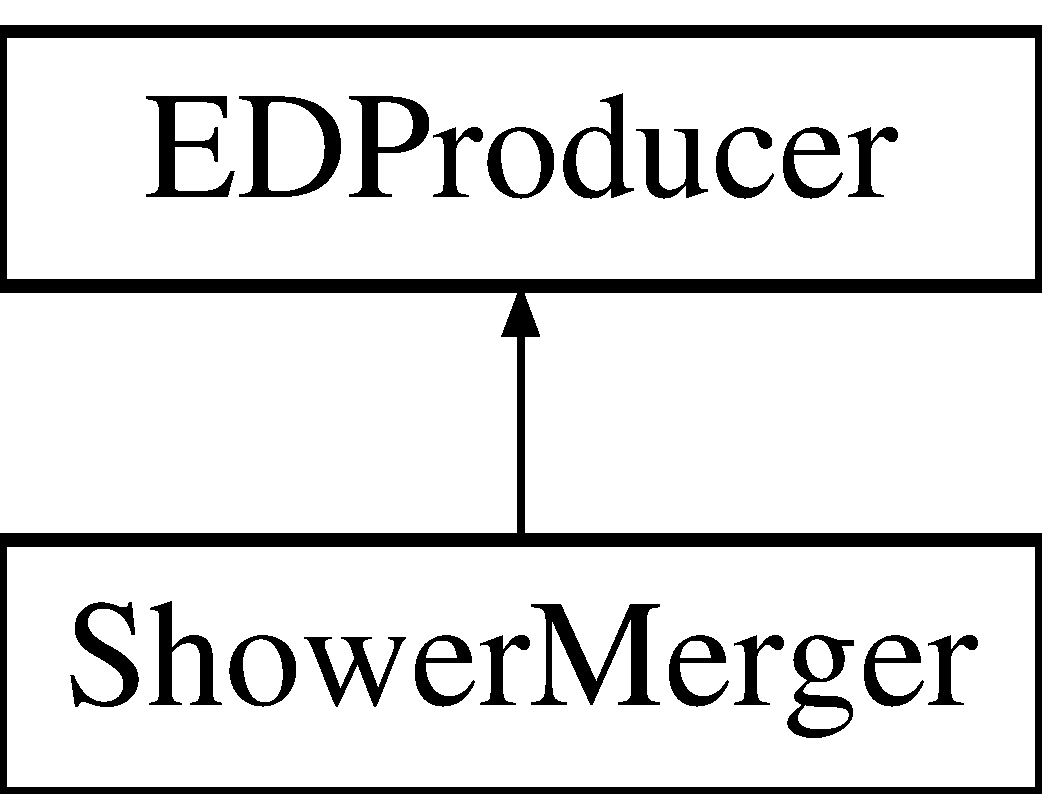
\includegraphics[height=2.000000cm]{classShowerMerger}
\end{center}
\end{figure}
\subsection*{Public Member Functions}
\begin{DoxyCompactItemize}
\item 
{\bfseries Shower\+Merger} (fhicl\+::\+Parameter\+Set const \&p)\hypertarget{classShowerMerger_a50fc7d6db9b3f84bba1d7e7e68f1374e}{}\label{classShowerMerger_a50fc7d6db9b3f84bba1d7e7e68f1374e}

\item 
{\bfseries Shower\+Merger} (\hyperlink{classShowerMerger}{Shower\+Merger} const \&)=delete\hypertarget{classShowerMerger_a2b781d7856276bf348a49fd0a06cb24f}{}\label{classShowerMerger_a2b781d7856276bf348a49fd0a06cb24f}

\item 
{\bfseries Shower\+Merger} (\hyperlink{classShowerMerger}{Shower\+Merger} \&\&)=delete\hypertarget{classShowerMerger_a080dc5947c74294bf05cb5df45743571}{}\label{classShowerMerger_a080dc5947c74294bf05cb5df45743571}

\item 
\hyperlink{classShowerMerger}{Shower\+Merger} \& {\bfseries operator=} (\hyperlink{classShowerMerger}{Shower\+Merger} const \&)=delete\hypertarget{classShowerMerger_aa2a1c38ecced6bf3708cf075cc871b07}{}\label{classShowerMerger_aa2a1c38ecced6bf3708cf075cc871b07}

\item 
\hyperlink{classShowerMerger}{Shower\+Merger} \& {\bfseries operator=} (\hyperlink{classShowerMerger}{Shower\+Merger} \&\&)=delete\hypertarget{classShowerMerger_a93a9e5d5251f530287fdd39f77584bf2}{}\label{classShowerMerger_a93a9e5d5251f530287fdd39f77584bf2}

\item 
void {\bfseries produce} (art\+::\+Event \&e) override\hypertarget{classShowerMerger_ab7251dd56c36d4d8ba07437af0b33bb9}{}\label{classShowerMerger_ab7251dd56c36d4d8ba07437af0b33bb9}

\item 
void {\bfseries begin\+Job} () override\hypertarget{classShowerMerger_a042daf0f57e3c5c0c08dc9274f98b63e}{}\label{classShowerMerger_a042daf0f57e3c5c0c08dc9274f98b63e}

\item 
void {\bfseries end\+Job} () override\hypertarget{classShowerMerger_a37852496f6771e29b167cd09c6c65cd0}{}\label{classShowerMerger_a37852496f6771e29b167cd09c6c65cd0}

\end{DoxyCompactItemize}
\subsection*{Private Member Functions}
\begin{DoxyCompactItemize}
\item 
void {\bfseries Reset\+T\+Tree} ()\hypertarget{classShowerMerger_a4529aa1606f5db0884cbbf23945ec98a}{}\label{classShowerMerger_a4529aa1606f5db0884cbbf23945ec98a}

\item 
bool {\bfseries Find\+Shower\+Branches} (const size\+\_\+t shr\+\_\+pfp\+\_\+idx, const std\+::vector$<$ searchingfornues\+::\+Proxy\+Pfp\+Elem\+\_\+t $>$ \&slice\+\_\+pfp\+\_\+v, std\+::vector$<$ size\+\_\+t $>$ \&branch\+\_\+pfp\+\_\+idx\+\_\+v)\hypertarget{classShowerMerger_a6fb74d3738dbaf29ebe0257eea8e3c6c}{}\label{classShowerMerger_a6fb74d3738dbaf29ebe0257eea8e3c6c}

\item 
bool {\bfseries Find\+Shower\+Trunk} (const size\+\_\+t shr\+\_\+pfp\+\_\+idx, const std\+::vector$<$ searchingfornues\+::\+Proxy\+Pfp\+Elem\+\_\+t $>$ \&slice\+\_\+pfp\+\_\+v, T\+Vector3 \&vtxcandidate, size\+\_\+t \&trktrunk\+\_\+pfp\+\_\+idx)\hypertarget{classShowerMerger_a559f4ef0334813f609ce0038fc5b273c}{}\label{classShowerMerger_a559f4ef0334813f609ce0038fc5b273c}

\item 
void \hyperlink{classShowerMerger_a9fb233f4aafc287d68e3f80bc5fcf27a}{Build\+P\+F\+P\+Map} (const searchingfornues\+::\+Proxy\+Pfp\+Coll\+\_\+t \&pfp\+\_\+pxy\+\_\+col)
\begin{DoxyCompactList}\small\item\em function to builf a map linking P\+F\+Particle index to Self() attribute \end{DoxyCompactList}\item 
void \hyperlink{classShowerMerger_af7fd315853bd22adcb9a9479706673de}{Add\+Daughters} (const searchingfornues\+::\+Proxy\+Pfp\+Elem\+\_\+t \&pfp\+\_\+pxy, const searchingfornues\+::\+Proxy\+Pfp\+Coll\+\_\+t \&pfp\+\_\+pxy\+\_\+col, std\+::vector$<$ searchingfornues\+::\+Proxy\+Pfp\+Elem\+\_\+t $>$ \&slice\+\_\+v)
\begin{DoxyCompactList}\small\item\em build P\+F\+Particle hierarchy (i.\+e. slice) from parent \mbox{[}recursive function\mbox{]} \end{DoxyCompactList}\item 
void {\bfseries Save\+Truth} (art\+::\+Event const \&e)\hypertarget{classShowerMerger_a2182bc1472f67f60cd02c7546fb0eabd}{}\label{classShowerMerger_a2182bc1472f67f60cd02c7546fb0eabd}

\end{DoxyCompactItemize}
\subsection*{Private Attributes}
\begin{DoxyCompactItemize}
\item 
art\+::\+Input\+Tag {\bfseries f\+M\+C\+Tproducer}\hypertarget{classShowerMerger_af9dd2ff006eefadb48b2a92c91cd2265}{}\label{classShowerMerger_af9dd2ff006eefadb48b2a92c91cd2265}

\item 
art\+::\+Input\+Tag {\bfseries f\+P\+F\+Pproducer}\hypertarget{classShowerMerger_af8b7771a13ec95338dd11ce067b13c22}{}\label{classShowerMerger_af8b7771a13ec95338dd11ce067b13c22}

\item 
art\+::\+Input\+Tag {\bfseries f\+C\+L\+Sproducer}\hypertarget{classShowerMerger_afb1c04a03669251c3cf1334c456dcf80}{}\label{classShowerMerger_afb1c04a03669251c3cf1334c456dcf80}

\item 
art\+::\+Input\+Tag {\bfseries f\+P\+C\+Aproducer}\hypertarget{classShowerMerger_ae69a8fc5e6a429f69d174bfd3f921c07}{}\label{classShowerMerger_ae69a8fc5e6a429f69d174bfd3f921c07}

\item 
art\+::\+Input\+Tag {\bfseries f\+S\+L\+Cproducer}\hypertarget{classShowerMerger_a182acfadf0569a8ac61297af22426b91}{}\label{classShowerMerger_a182acfadf0569a8ac61297af22426b91}

\item 
art\+::\+Input\+Tag {\bfseries f\+H\+I\+Tproducer}\hypertarget{classShowerMerger_af16d85668db5d9385d9be168fbf793ac}{}\label{classShowerMerger_af16d85668db5d9385d9be168fbf793ac}

\item 
art\+::\+Input\+Tag {\bfseries f\+S\+H\+Rproducer}\hypertarget{classShowerMerger_aab960097c76033faec9afaef1816f8ea}{}\label{classShowerMerger_aab960097c76033faec9afaef1816f8ea}

\item 
art\+::\+Input\+Tag {\bfseries f\+V\+T\+Xproducer}\hypertarget{classShowerMerger_aca02202f54f7d452f77acbac9effa37a}{}\label{classShowerMerger_aca02202f54f7d452f77acbac9effa37a}

\item 
art\+::\+Input\+Tag {\bfseries f\+T\+R\+Kproducer}\hypertarget{classShowerMerger_a5a86d972b7d5858a9c1c0e2bf1a0990d}{}\label{classShowerMerger_a5a86d972b7d5858a9c1c0e2bf1a0990d}

\item 
art\+::\+Input\+Tag {\bfseries f\+S\+P\+Pproducer}\hypertarget{classShowerMerger_aef6fe39020ddb33b937479a36bb3ba3b}{}\label{classShowerMerger_aef6fe39020ddb33b937479a36bb3ba3b}

\item 
float {\bfseries f\+Shr\+Vtx\+Trk\+Dist\+Max}\hypertarget{classShowerMerger_a292711d76adde897b3f56d34749c9e81}{}\label{classShowerMerger_a292711d76adde897b3f56d34749c9e81}

\item 
float {\bfseries f\+Shr\+Trk\+Dot\+Min}\hypertarget{classShowerMerger_a8ec6d21e5306f14c7f55dc511b96cb0e}{}\label{classShowerMerger_a8ec6d21e5306f14c7f55dc511b96cb0e}

\item 
float {\bfseries f\+Min\+Branch\+Cone\+Dot}\hypertarget{classShowerMerger_ab4b67c77e7d80adab4ad82c2dd34d673}{}\label{classShowerMerger_ab4b67c77e7d80adab4ad82c2dd34d673}

\item 
float {\bfseries f\+Min\+Branch\+Vtx\+Dist}\hypertarget{classShowerMerger_abd7e2289632835a7d31f2d003df914e2}{}\label{classShowerMerger_abd7e2289632835a7d31f2d003df914e2}

\item 
T\+Tree $\ast$ {\bfseries \+\_\+tree}\hypertarget{classShowerMerger_a82c7611662695dbe3e362f1f5a2d98e5}{}\label{classShowerMerger_a82c7611662695dbe3e362f1f5a2d98e5}

\item 
float {\bfseries \+\_\+nu\+\_\+e}\hypertarget{classShowerMerger_ab3f07b21a270a90c57b2e77676f9866c}{}\label{classShowerMerger_ab3f07b21a270a90c57b2e77676f9866c}

\item 
float {\bfseries \+\_\+elec\+\_\+e}\hypertarget{classShowerMerger_ad1065d4ed52c3ae03d0cf38952573231}{}\label{classShowerMerger_ad1065d4ed52c3ae03d0cf38952573231}

\item 
int {\bfseries \+\_\+nelec}\hypertarget{classShowerMerger_aa2145f5a2d6367a211d9f18b922dd3f6}{}\label{classShowerMerger_aa2145f5a2d6367a211d9f18b922dd3f6}

\item 
int {\bfseries \+\_\+nreco}\hypertarget{classShowerMerger_ad68280897010717c7448eca8996345b3}{}\label{classShowerMerger_ad68280897010717c7448eca8996345b3}

\item 
float {\bfseries \+\_\+vtx\+\_\+x}\hypertarget{classShowerMerger_ab7c8c6dcebe9d4fa89849f9aca5f026f}{}\label{classShowerMerger_ab7c8c6dcebe9d4fa89849f9aca5f026f}

\item 
float {\bfseries \+\_\+vtx\+\_\+y}\hypertarget{classShowerMerger_a2e8e72e16c4952f2303aa54e0dcc4a3c}{}\label{classShowerMerger_a2e8e72e16c4952f2303aa54e0dcc4a3c}

\item 
float {\bfseries \+\_\+vtx\+\_\+z}\hypertarget{classShowerMerger_ace62492811b2651dc24aca3fbdbf98ef}{}\label{classShowerMerger_ace62492811b2651dc24aca3fbdbf98ef}

\item 
float {\bfseries \+\_\+vtx\+\_\+t}\hypertarget{classShowerMerger_a1a1af576166ea128395fc39e9d1c781c}{}\label{classShowerMerger_a1a1af576166ea128395fc39e9d1c781c}

\item 
float {\bfseries \+\_\+rc\+\_\+vtx\+\_\+x}\hypertarget{classShowerMerger_a1da4fe3ad72b0a272a429600f807c0a5}{}\label{classShowerMerger_a1da4fe3ad72b0a272a429600f807c0a5}

\item 
float {\bfseries \+\_\+rc\+\_\+vtx\+\_\+y}\hypertarget{classShowerMerger_ae94742dcf3972e0ffeccb3a830e16410}{}\label{classShowerMerger_ae94742dcf3972e0ffeccb3a830e16410}

\item 
float {\bfseries \+\_\+rc\+\_\+vtx\+\_\+z}\hypertarget{classShowerMerger_afe0e973a8932863f447c7d3779b3467e}{}\label{classShowerMerger_afe0e973a8932863f447c7d3779b3467e}

\item 
float {\bfseries \+\_\+\+Ashr\+\_\+x}\hypertarget{classShowerMerger_ae3b9eb8b3ad423db53ff9566ef1569e8}{}\label{classShowerMerger_ae3b9eb8b3ad423db53ff9566ef1569e8}

\item 
float {\bfseries \+\_\+\+Ashr\+\_\+y}\hypertarget{classShowerMerger_ae79b65a1d3a44f50eea164214be429f0}{}\label{classShowerMerger_ae79b65a1d3a44f50eea164214be429f0}

\item 
float {\bfseries \+\_\+\+Ashr\+\_\+z}\hypertarget{classShowerMerger_a05a76786171800883f65d36298eb1deb}{}\label{classShowerMerger_a05a76786171800883f65d36298eb1deb}

\item 
float {\bfseries \+\_\+\+Ashr\+\_\+q}\hypertarget{classShowerMerger_a990b5530d998133fd0bd4dba49c027bf}{}\label{classShowerMerger_a990b5530d998133fd0bd4dba49c027bf}

\item 
float {\bfseries \+\_\+\+Pshr\+\_\+x}\hypertarget{classShowerMerger_ac7452680134b4d808e0292bb4e5d7ebe}{}\label{classShowerMerger_ac7452680134b4d808e0292bb4e5d7ebe}

\item 
float {\bfseries \+\_\+\+Pshr\+\_\+y}\hypertarget{classShowerMerger_a43b9620bb7b263478345b51e752cb4a2}{}\label{classShowerMerger_a43b9620bb7b263478345b51e752cb4a2}

\item 
float {\bfseries \+\_\+\+Pshr\+\_\+z}\hypertarget{classShowerMerger_af8094f3e46f6a4747a330afc1d2dc303}{}\label{classShowerMerger_af8094f3e46f6a4747a330afc1d2dc303}

\item 
float {\bfseries \+\_\+\+Pshr\+\_\+q}\hypertarget{classShowerMerger_ae2945b4d342ec4f487ed4798f017dd45}{}\label{classShowerMerger_ae2945b4d342ec4f487ed4798f017dd45}

\item 
float {\bfseries \+\_\+xtimeoffset}\hypertarget{classShowerMerger_a98adeb9a7abfcc0c4126f3c2fa394f26}{}\label{classShowerMerger_a98adeb9a7abfcc0c4126f3c2fa394f26}

\item 
float {\bfseries \+\_\+xsceoffset}\hypertarget{classShowerMerger_a060965f5293a88e921f4fcfc73494878}{}\label{classShowerMerger_a060965f5293a88e921f4fcfc73494878}

\item 
float {\bfseries \+\_\+ysceoffset}\hypertarget{classShowerMerger_a544004d4470bf7ead4c176685d58cfd6}{}\label{classShowerMerger_a544004d4470bf7ead4c176685d58cfd6}

\item 
float {\bfseries \+\_\+zsceoffset}\hypertarget{classShowerMerger_aa010b54e82a6bb0381946d7c064a9e7e}{}\label{classShowerMerger_aa010b54e82a6bb0381946d7c064a9e7e}

\item 
std\+::map$<$ unsigned int, unsigned int $>$ {\bfseries \+\_\+pfpmap}\hypertarget{classShowerMerger_ad0e0ff1fb206209963efb0690a3e9504}{}\label{classShowerMerger_ad0e0ff1fb206209963efb0690a3e9504}

\end{DoxyCompactItemize}


\subsection{Member Function Documentation}
\index{Shower\+Merger@{Shower\+Merger}!Add\+Daughters@{Add\+Daughters}}
\index{Add\+Daughters@{Add\+Daughters}!Shower\+Merger@{Shower\+Merger}}
\subsubsection[{\texorpdfstring{Add\+Daughters(const searchingfornues\+::\+Proxy\+Pfp\+Elem\+\_\+t \&pfp\+\_\+pxy, const searchingfornues\+::\+Proxy\+Pfp\+Coll\+\_\+t \&pfp\+\_\+pxy\+\_\+col, std\+::vector$<$ searchingfornues\+::\+Proxy\+Pfp\+Elem\+\_\+t $>$ \&slice\+\_\+v)}{AddDaughters(const searchingfornues::ProxyPfpElem_t &pfp_pxy, const searchingfornues::ProxyPfpColl_t &pfp_pxy_col, std::vector< searchingfornues::ProxyPfpElem_t > &slice_v)}}]{\setlength{\rightskip}{0pt plus 5cm}void Shower\+Merger\+::\+Add\+Daughters (
\begin{DoxyParamCaption}
\item[{const searchingfornues\+::\+Proxy\+Pfp\+Elem\+\_\+t \&}]{pfp\+\_\+pxy, }
\item[{const searchingfornues\+::\+Proxy\+Pfp\+Coll\+\_\+t \&}]{pfp\+\_\+pxy\+\_\+col, }
\item[{std\+::vector$<$ searchingfornues\+::\+Proxy\+Pfp\+Elem\+\_\+t $>$ \&}]{slice\+\_\+v}
\end{DoxyParamCaption}
)\hspace{0.3cm}{\ttfamily [private]}}\hypertarget{classShowerMerger_af7fd315853bd22adcb9a9479706673de}{}\label{classShowerMerger_af7fd315853bd22adcb9a9479706673de}


build P\+F\+Particle hierarchy (i.\+e. slice) from parent \mbox{[}recursive function\mbox{]} 

pfp\+\_\+pxy \+: parent pfparticle proxy for which to add daughters  pfp\+\_\+pxy\+\_\+col \+: evnt P\+FP proxy collection  slice\+\_\+v \+: passed by reference, slice containing all P\+F\+Particles in hierarchy \index{Shower\+Merger@{Shower\+Merger}!Build\+P\+F\+P\+Map@{Build\+P\+F\+P\+Map}}
\index{Build\+P\+F\+P\+Map@{Build\+P\+F\+P\+Map}!Shower\+Merger@{Shower\+Merger}}
\subsubsection[{\texorpdfstring{Build\+P\+F\+P\+Map(const searchingfornues\+::\+Proxy\+Pfp\+Coll\+\_\+t \&pfp\+\_\+pxy\+\_\+col)}{BuildPFPMap(const searchingfornues::ProxyPfpColl_t &pfp_pxy_col)}}]{\setlength{\rightskip}{0pt plus 5cm}void Shower\+Merger\+::\+Build\+P\+F\+P\+Map (
\begin{DoxyParamCaption}
\item[{const searchingfornues\+::\+Proxy\+Pfp\+Coll\+\_\+t \&}]{pfp\+\_\+pxy\+\_\+col}
\end{DoxyParamCaption}
)\hspace{0.3cm}{\ttfamily [private]}}\hypertarget{classShowerMerger_a9fb233f4aafc287d68e3f80bc5fcf27a}{}\label{classShowerMerger_a9fb233f4aafc287d68e3f80bc5fcf27a}


function to builf a map linking P\+F\+Particle index to Self() attribute 

handle to event pfparticle record 

The documentation for this class was generated from the following file\+:\begin{DoxyCompactItemize}
\item 
/home/travis/build/ubneutrinos/searchingfornues/\+Shower\+Reco/Shower\+Merger\+\_\+module.\+cc\end{DoxyCompactItemize}

\hypertarget{classselection_1_1ShowerSelection}{}\section{selection\+:\+:Shower\+Selection Class Reference}
\label{classselection_1_1ShowerSelection}\index{selection\+::\+Shower\+Selection@{selection\+::\+Shower\+Selection}}
Inheritance diagram for selection\+:\+:Shower\+Selection\+:\begin{figure}[H]
\begin{center}
\leavevmode
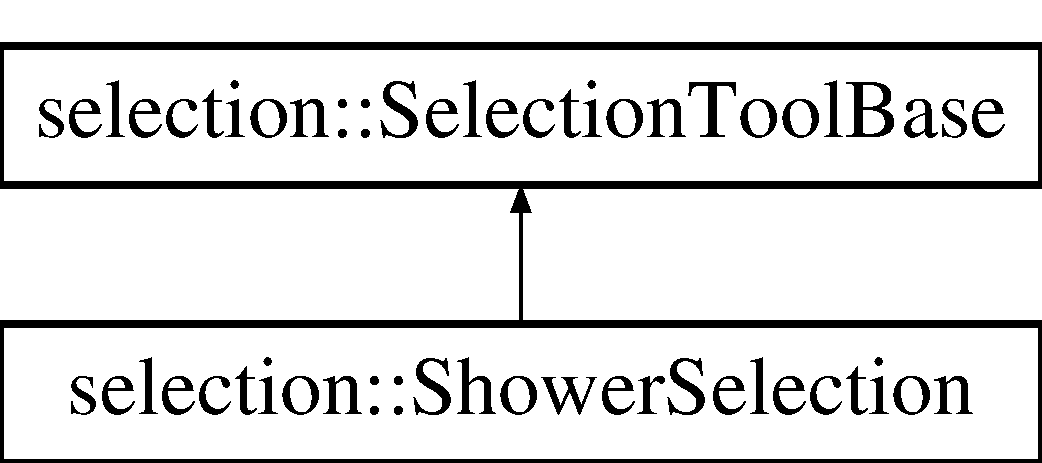
\includegraphics[height=2.000000cm]{classselection_1_1ShowerSelection}
\end{center}
\end{figure}
\subsection*{Public Member Functions}
\begin{DoxyCompactItemize}
\item 
\hyperlink{classselection_1_1ShowerSelection_a07b97cd199fb1eba72923555c4d05ec7}{Shower\+Selection} (const fhicl\+::\+Parameter\+Set \&pset)
\begin{DoxyCompactList}\small\item\em Constructor. \end{DoxyCompactList}\item 
\hyperlink{classselection_1_1ShowerSelection_a59328cc3ca5b6875244f1d2c6a2f3b8e}{$\sim$\+Shower\+Selection} ()\hypertarget{classselection_1_1ShowerSelection_a59328cc3ca5b6875244f1d2c6a2f3b8e}{}\label{classselection_1_1ShowerSelection_a59328cc3ca5b6875244f1d2c6a2f3b8e}

\begin{DoxyCompactList}\small\item\em Destructor. \end{DoxyCompactList}\item 
void \hyperlink{classselection_1_1ShowerSelection_a723729db901f048f4fcb5501895305eb}{configure} (fhicl\+::\+Parameter\+Set const \&pset)
\item 
bool \hyperlink{classselection_1_1ShowerSelection_aa538b905ab6e8a329acf3eaa97cc0af9}{select\+Event} (art\+::\+Event const \&e, const std\+::vector$<$ Proxy\+Pfp\+Elem\+\_\+t $>$ \&pfp\+\_\+pxy\+\_\+v)
\begin{DoxyCompactList}\small\item\em Selection function. \end{DoxyCompactList}\item 
void \hyperlink{classselection_1_1ShowerSelection_a1ea09a0f7da6a3e7b9f1eb9728bff1cf}{set\+Branches} (T\+Tree $\ast$\+\_\+tree)\hypertarget{classselection_1_1ShowerSelection_a1ea09a0f7da6a3e7b9f1eb9728bff1cf}{}\label{classselection_1_1ShowerSelection_a1ea09a0f7da6a3e7b9f1eb9728bff1cf}

\begin{DoxyCompactList}\small\item\em set branches for T\+Tree \end{DoxyCompactList}\item 
void \hyperlink{classselection_1_1ShowerSelection_a9d35d47af8468781d97c4e872c96d768}{reset\+T\+Tree} (T\+Tree $\ast$\+\_\+tree)\hypertarget{classselection_1_1ShowerSelection_a9d35d47af8468781d97c4e872c96d768}{}\label{classselection_1_1ShowerSelection_a9d35d47af8468781d97c4e872c96d768}

\begin{DoxyCompactList}\small\item\em reset ttree branches \end{DoxyCompactList}\item 
void \hyperlink{classselection_1_1ShowerSelection_aa790f42dca70058f567f15e130627011}{Reset} ()\hypertarget{classselection_1_1ShowerSelection_aa790f42dca70058f567f15e130627011}{}\label{classselection_1_1ShowerSelection_aa790f42dca70058f567f15e130627011}

\begin{DoxyCompactList}\small\item\em reset module \end{DoxyCompactList}\end{DoxyCompactItemize}
\subsection*{Private Member Functions}
\begin{DoxyCompactItemize}
\item 
void {\bfseries Track\+Fitd\+Edx} (const searchingfornues\+::\+Proxy\+Calo\+Elem\+\_\+t \&trk, float \&dedxU, float \&dedxV, float \&dedxY)\hypertarget{classselection_1_1ShowerSelection_a9cf0d6d41063cb9137db9d37500be7dd}{}\label{classselection_1_1ShowerSelection_a9cf0d6d41063cb9137db9d37500be7dd}

\item 
void \hyperlink{classselection_1_1ShowerSelection_a9f007d4be7a578b6d07db9172ad4ab14}{Store\+Vertex} (const Proxy\+Pfp\+Elem\+\_\+t \&pfp\+\_\+pxy, T\+Vector3 \&nuvtx)\hypertarget{classselection_1_1ShowerSelection_a9f007d4be7a578b6d07db9172ad4ab14}{}\label{classselection_1_1ShowerSelection_a9f007d4be7a578b6d07db9172ad4ab14}

\begin{DoxyCompactList}\small\item\em given a P\+FP (the neutrino one) grab the associated vertex and store vertex by reference \end{DoxyCompactList}\item 
float {\bfseries Get\+Track\+Shower\+Score} (const Proxy\+Pfp\+Elem\+\_\+t \&pfp\+\_\+pxy)\hypertarget{classselection_1_1ShowerSelection_aa4c7b1935b0705093c8be5065a2d25ed}{}\label{classselection_1_1ShowerSelection_aa4c7b1935b0705093c8be5065a2d25ed}

\end{DoxyCompactItemize}
\subsection*{Private Attributes}
\begin{DoxyCompactItemize}
\item 
int {\bfseries \+\_\+run}\hypertarget{classselection_1_1ShowerSelection_af3dfe27ba53744ad650ffcfe6e09e9ce}{}\label{classselection_1_1ShowerSelection_af3dfe27ba53744ad650ffcfe6e09e9ce}

\item 
int {\bfseries \+\_\+sub}\hypertarget{classselection_1_1ShowerSelection_af26a13ed100df860be1ace437e3a55ec}{}\label{classselection_1_1ShowerSelection_af26a13ed100df860be1ace437e3a55ec}

\item 
int {\bfseries \+\_\+evt}\hypertarget{classselection_1_1ShowerSelection_aea5f29f1c64ea394ff977b19df88706f}{}\label{classselection_1_1ShowerSelection_aea5f29f1c64ea394ff977b19df88706f}

\item 
int {\bfseries \+\_\+nshower}\hypertarget{classselection_1_1ShowerSelection_a61892b39930f340e6e869707cb40b1a6}{}\label{classselection_1_1ShowerSelection_a61892b39930f340e6e869707cb40b1a6}

\item 
int {\bfseries \+\_\+ntrack}\hypertarget{classselection_1_1ShowerSelection_abd4e9031fc17ec7d447d5bc29237b01a}{}\label{classselection_1_1ShowerSelection_abd4e9031fc17ec7d447d5bc29237b01a}

\item 
int {\bfseries \+\_\+nupdgreco}\hypertarget{classselection_1_1ShowerSelection_adb663ffb64456c3b652d22460d4d7047}{}\label{classselection_1_1ShowerSelection_adb663ffb64456c3b652d22460d4d7047}

\item 
float {\bfseries \+\_\+maxtrklen}\hypertarget{classselection_1_1ShowerSelection_a9fac735cbf38a99c3cdb52aa61a3f5d6}{}\label{classselection_1_1ShowerSelection_a9fac735cbf38a99c3cdb52aa61a3f5d6}

\item 
float {\bfseries \+\_\+shr\+\_\+score}\hypertarget{classselection_1_1ShowerSelection_a018104d30f773a2d8a3187197f0de81b}{}\label{classselection_1_1ShowerSelection_a018104d30f773a2d8a3187197f0de81b}

\item 
float {\bfseries \+\_\+shr\+\_\+energy\+\_\+Y}\hypertarget{classselection_1_1ShowerSelection_a2ffda067ae39e512f913bbedaeed401e}{}\label{classselection_1_1ShowerSelection_a2ffda067ae39e512f913bbedaeed401e}

\item 
float {\bfseries \+\_\+shr\+\_\+energy\+\_\+V}\hypertarget{classselection_1_1ShowerSelection_a17ab853b88beb71102fac8504fec4268}{}\label{classselection_1_1ShowerSelection_a17ab853b88beb71102fac8504fec4268}

\item 
float {\bfseries \+\_\+shr\+\_\+energy\+\_\+U}\hypertarget{classselection_1_1ShowerSelection_ad45d91e1d71b9fea3aa65bf07fe5b2b3}{}\label{classselection_1_1ShowerSelection_ad45d91e1d71b9fea3aa65bf07fe5b2b3}

\item 
float {\bfseries \+\_\+shr\+\_\+dedx\+\_\+Y}\hypertarget{classselection_1_1ShowerSelection_a1a2d2a155400549bac972a0faf999494}{}\label{classselection_1_1ShowerSelection_a1a2d2a155400549bac972a0faf999494}

\item 
float {\bfseries \+\_\+shr\+\_\+dedx\+\_\+V}\hypertarget{classselection_1_1ShowerSelection_aa9b0c099e5f831864cd44ace8e055957}{}\label{classselection_1_1ShowerSelection_aa9b0c099e5f831864cd44ace8e055957}

\item 
float {\bfseries \+\_\+shr\+\_\+dedx\+\_\+U}\hypertarget{classselection_1_1ShowerSelection_a6f3b7dba2f0ebc492efcf48d805eb602}{}\label{classselection_1_1ShowerSelection_a6f3b7dba2f0ebc492efcf48d805eb602}

\item 
float {\bfseries \+\_\+shr\+\_\+dedx\+\_\+fit\+\_\+Y}\hypertarget{classselection_1_1ShowerSelection_ad50bf825fa5ee3fdb2b821770b2aa5cd}{}\label{classselection_1_1ShowerSelection_ad50bf825fa5ee3fdb2b821770b2aa5cd}

\item 
float {\bfseries \+\_\+shr\+\_\+dedx\+\_\+fit\+\_\+V}\hypertarget{classselection_1_1ShowerSelection_a1ef8d85de723f1de698db73e9f39746e}{}\label{classselection_1_1ShowerSelection_a1ef8d85de723f1de698db73e9f39746e}

\item 
float {\bfseries \+\_\+shr\+\_\+dedx\+\_\+fit\+\_\+U}\hypertarget{classselection_1_1ShowerSelection_a2f1221e97e38ff069830f7255bebc237}{}\label{classselection_1_1ShowerSelection_a2f1221e97e38ff069830f7255bebc237}

\item 
float {\bfseries \+\_\+shr\+\_\+dist}\hypertarget{classselection_1_1ShowerSelection_af3564629f032f48d86f256015ad9f64e}{}\label{classselection_1_1ShowerSelection_af3564629f032f48d86f256015ad9f64e}

\item 
float {\bfseries \+\_\+shr\+\_\+x}\hypertarget{classselection_1_1ShowerSelection_a4e1a5f0cb830990b6b62014de57f4335}{}\label{classselection_1_1ShowerSelection_a4e1a5f0cb830990b6b62014de57f4335}

\item 
float {\bfseries \+\_\+shr\+\_\+y}\hypertarget{classselection_1_1ShowerSelection_a0f632f8445e6cc9993a2f2df9d03804a}{}\label{classselection_1_1ShowerSelection_a0f632f8445e6cc9993a2f2df9d03804a}

\item 
float {\bfseries \+\_\+shr\+\_\+z}\hypertarget{classselection_1_1ShowerSelection_abd94487a568b61515d1dd98e8d68c2b2}{}\label{classselection_1_1ShowerSelection_abd94487a568b61515d1dd98e8d68c2b2}

\item 
float {\bfseries \+\_\+shr\+\_\+px}\hypertarget{classselection_1_1ShowerSelection_a9e37701dfc18e9e9d953ed6513bef260}{}\label{classselection_1_1ShowerSelection_a9e37701dfc18e9e9d953ed6513bef260}

\item 
float {\bfseries \+\_\+shr\+\_\+py}\hypertarget{classselection_1_1ShowerSelection_af1a9676b2eb26d0c70c463f7092914ae}{}\label{classselection_1_1ShowerSelection_af1a9676b2eb26d0c70c463f7092914ae}

\item 
float {\bfseries \+\_\+shr\+\_\+pz}\hypertarget{classselection_1_1ShowerSelection_af701aae8694be9339ced383ccbc0b999}{}\label{classselection_1_1ShowerSelection_af701aae8694be9339ced383ccbc0b999}

\item 
size\+\_\+t {\bfseries \+\_\+shr\+\_\+maxe\+\_\+pfp\+\_\+i}\hypertarget{classselection_1_1ShowerSelection_aed0d279cec89fbc428d9e59df7fb9f09}{}\label{classselection_1_1ShowerSelection_aed0d279cec89fbc428d9e59df7fb9f09}

\item 
float {\bfseries f\+Trk\+Shrscore}\hypertarget{classselection_1_1ShowerSelection_a2af278b93c55ba7eb0c9266e50a7c5bc}{}\label{classselection_1_1ShowerSelection_a2af278b93c55ba7eb0c9266e50a7c5bc}

\item 
float {\bfseries f\+Shrdedxmax}\hypertarget{classselection_1_1ShowerSelection_a470499e9d5ac01695e2484f475734300}{}\label{classselection_1_1ShowerSelection_a470499e9d5ac01695e2484f475734300}

\item 
float {\bfseries f\+Shr\+Radlen}\hypertarget{classselection_1_1ShowerSelection_ac97e2dd5963ae97983d98424bef0ec20}{}\label{classselection_1_1ShowerSelection_ac97e2dd5963ae97983d98424bef0ec20}

\item 
float {\bfseries f\+Shr\+Energy}\hypertarget{classselection_1_1ShowerSelection_a033c15eae1bbdeb65df67c79a0b815fd}{}\label{classselection_1_1ShowerSelection_a033c15eae1bbdeb65df67c79a0b815fd}

\item 
float {\bfseries f\+Max\+Trklen}\hypertarget{classselection_1_1ShowerSelection_a3cbe6b998a95bf55da6ef1a94bdac9c0}{}\label{classselection_1_1ShowerSelection_a3cbe6b998a95bf55da6ef1a94bdac9c0}

\item 
art\+::\+Input\+Tag {\bfseries f\+T\+R\+Kproducer}\hypertarget{classselection_1_1ShowerSelection_a681be5a0cf499e8ac32078ab941fc9e1}{}\label{classselection_1_1ShowerSelection_a681be5a0cf499e8ac32078ab941fc9e1}

\item 
art\+::\+Input\+Tag {\bfseries f\+C\+A\+Lproducer}\hypertarget{classselection_1_1ShowerSelection_acb7a3a664589240707094c08825d4383}{}\label{classselection_1_1ShowerSelection_acb7a3a664589240707094c08825d4383}

\end{DoxyCompactItemize}
\subsection*{Additional Inherited Members}


\subsection{Constructor \& Destructor Documentation}
\index{selection\+::\+Shower\+Selection@{selection\+::\+Shower\+Selection}!Shower\+Selection@{Shower\+Selection}}
\index{Shower\+Selection@{Shower\+Selection}!selection\+::\+Shower\+Selection@{selection\+::\+Shower\+Selection}}
\subsubsection[{\texorpdfstring{Shower\+Selection(const fhicl\+::\+Parameter\+Set \&pset)}{ShowerSelection(const fhicl::ParameterSet &pset)}}]{\setlength{\rightskip}{0pt plus 5cm}selection\+::\+Shower\+Selection\+::\+Shower\+Selection (
\begin{DoxyParamCaption}
\item[{const fhicl\+::\+Parameter\+Set \&}]{pset}
\end{DoxyParamCaption}
)}\hypertarget{classselection_1_1ShowerSelection_a07b97cd199fb1eba72923555c4d05ec7}{}\label{classselection_1_1ShowerSelection_a07b97cd199fb1eba72923555c4d05ec7}


Constructor. 


\begin{DoxyParams}{Parameters}
{\em pset} & Constructor.\\
\hline
\end{DoxyParams}
Arguments\+:

pset -\/ Fcl parameters. 

\subsection{Member Function Documentation}
\index{selection\+::\+Shower\+Selection@{selection\+::\+Shower\+Selection}!configure@{configure}}
\index{configure@{configure}!selection\+::\+Shower\+Selection@{selection\+::\+Shower\+Selection}}
\subsubsection[{\texorpdfstring{configure(fhicl\+::\+Parameter\+Set const \&pset)}{configure(fhicl::ParameterSet const &pset)}}]{\setlength{\rightskip}{0pt plus 5cm}void selection\+::\+Shower\+Selection\+::configure (
\begin{DoxyParamCaption}
\item[{fhicl\+::\+Parameter\+Set const \&}]{pset}
\end{DoxyParamCaption}
)}\hypertarget{classselection_1_1ShowerSelection_a723729db901f048f4fcb5501895305eb}{}\label{classselection_1_1ShowerSelection_a723729db901f048f4fcb5501895305eb}
Reconfigure method.

Arguments\+:

pset -\/ Fcl parameter set. \index{selection\+::\+Shower\+Selection@{selection\+::\+Shower\+Selection}!select\+Event@{select\+Event}}
\index{select\+Event@{select\+Event}!selection\+::\+Shower\+Selection@{selection\+::\+Shower\+Selection}}
\subsubsection[{\texorpdfstring{select\+Event(art\+::\+Event const \&e, const std\+::vector$<$ Proxy\+Pfp\+Elem\+\_\+t $>$ \&pfp\+\_\+pxy\+\_\+v)}{selectEvent(art::Event const &e, const std::vector< ProxyPfpElem_t > &pfp_pxy_v)}}]{\setlength{\rightskip}{0pt plus 5cm}bool selection\+::\+Shower\+Selection\+::select\+Event (
\begin{DoxyParamCaption}
\item[{art\+::\+Event const \&}]{e, }
\item[{const std\+::vector$<$ Proxy\+Pfp\+Elem\+\_\+t $>$ \&}]{pfp\+\_\+pxy\+\_\+v}
\end{DoxyParamCaption}
)\hspace{0.3cm}{\ttfamily [virtual]}}\hypertarget{classselection_1_1ShowerSelection_aa538b905ab6e8a329acf3eaa97cc0af9}{}\label{classselection_1_1ShowerSelection_aa538b905ab6e8a329acf3eaa97cc0af9}


Selection function. 

select\+Event

Arguments\+:

art\+::\+Event slice track pointer vector slice shower pointer vector 

Implements \hyperlink{classselection_1_1SelectionToolBase_ab63818dac49b43418fe9eb3b8cd98c9c}{selection\+::\+Selection\+Tool\+Base}.



The documentation for this class was generated from the following file\+:\begin{DoxyCompactItemize}
\item 
/home/travis/build/ubneutrinos/searchingfornues/\+Selection/\+Selection\+Tools/Shower\+Selection\+\_\+tool.\+cc\end{DoxyCompactItemize}

\hypertarget{classflashmatch_1_1FlashMatchingTool_1_1SliceCandidate}{}\section{flashmatch\+:\+:Flash\+Matching\+Tool\+:\+:Slice\+Candidate Class Reference}
\label{classflashmatch_1_1FlashMatchingTool_1_1SliceCandidate}\index{flashmatch\+::\+Flash\+Matching\+Tool\+::\+Slice\+Candidate@{flashmatch\+::\+Flash\+Matching\+Tool\+::\+Slice\+Candidate}}


A candidate for the target slice.  


\subsection*{Classes}
\begin{DoxyCompactItemize}
\item 
class \hyperlink{classflashmatch_1_1FlashMatchingTool_1_1SliceCandidate_1_1Deposition}{Deposition}
\begin{DoxyCompactList}\small\item\em Data to describe an amount of charge deposited in a given 3D position. \end{DoxyCompactList}\end{DoxyCompactItemize}
\subsection*{Public Types}
\begin{DoxyCompactItemize}
\item 
typedef std\+::vector$<$ \hyperlink{classflashmatch_1_1FlashMatchingTool_1_1SliceCandidate_1_1Deposition}{Deposition} $>$ {\bfseries Deposition\+Vector}\hypertarget{classflashmatch_1_1FlashMatchingTool_1_1SliceCandidate_aa57131c7a2914bae3315c3dae1dc9e9f}{}\label{classflashmatch_1_1FlashMatchingTool_1_1SliceCandidate_aa57131c7a2914bae3315c3dae1dc9e9f}

\end{DoxyCompactItemize}
\subsection*{Public Member Functions}
\begin{DoxyCompactItemize}
\item 
\hyperlink{classflashmatch_1_1FlashMatchingTool_1_1SliceCandidate_ae2d99f84ab9976ff1880906fa46427c2}{Slice\+Candidate} ()\hypertarget{classflashmatch_1_1FlashMatchingTool_1_1SliceCandidate_ae2d99f84ab9976ff1880906fa46427c2}{}\label{classflashmatch_1_1FlashMatchingTool_1_1SliceCandidate_ae2d99f84ab9976ff1880906fa46427c2}

\begin{DoxyCompactList}\small\item\em Default constructor. \end{DoxyCompactList}\item 
\hyperlink{classflashmatch_1_1FlashMatchingTool_1_1SliceCandidate_a5087a8ac4efb368f39643468585f7591}{Slice\+Candidate} (const std\+::vector$<$ art\+::\+Ptr$<$ recob\+::\+P\+F\+Particle $>$$>$ \&pfp\+\_\+v, const std\+::vector$<$ std\+::vector$<$ art\+::\+Ptr$<$ recob\+::\+Space\+Point $>$ $>$ $>$ \&spacepoint\+\_\+v\+\_\+v, const std\+::vector$<$ std\+::vector$<$ art\+::\+Ptr$<$ recob\+::\+Hit $>$ $>$ $>$ \&hit\+\_\+v\+\_\+v, const float charge\+To\+N\+Photons\+Track, const float charge\+To\+N\+Photons\+Shower)
\begin{DoxyCompactList}\small\item\em Parametrized constructor. \end{DoxyCompactList}\item 
{\bfseries Slice\+Candidate} (const std\+::vector$<$ art\+::\+Ptr$<$ recob\+::\+Space\+Point $>$ $>$ \&spacepoint\+\_\+v, const std\+::vector$<$ art\+::\+Ptr$<$ recob\+::\+Hit $>$ $>$ \&hit\+\_\+v, const float charge\+To\+N\+Photons\+Track, const float charge\+To\+N\+Photons\+Shower)\hypertarget{classflashmatch_1_1FlashMatchingTool_1_1SliceCandidate_a9ba86dbafd572849c898422aee9dddda}{}\label{classflashmatch_1_1FlashMatchingTool_1_1SliceCandidate_a9ba86dbafd572849c898422aee9dddda}

\item 
bool \hyperlink{classflashmatch_1_1FlashMatchingTool_1_1SliceCandidate_ac39549da77f9d1d2fef87dd31a01e09a}{Is\+Compatible\+With\+Beam\+Flash} (const \hyperlink{classflashmatch_1_1FlashMatchingTool_1_1FlashCandidate}{Flash\+Candidate} \&beam\+Flash, const float max\+DeltaY, const float max\+DeltaZ, const float max\+Delta\+Y\+Sigma, const float max\+Delta\+Z\+Sigma, const float min\+Charge\+To\+Light\+Ratio, const float max\+Charge\+To\+Light\+Ratio)
\item 
float \hyperlink{classflashmatch_1_1FlashMatchingTool_1_1SliceCandidate_a7c1f2eedf7f2fc763cd7d738a5ac32af}{Get\+Flash\+Match\+Score} (\hyperlink{classflashmatch_1_1FlashMatchingTool_1_1FlashCandidate}{Flash\+Candidate} \&beam\+Flash, flashana\+::\+Flash\+Match\+Manager \&flash\+Match\+Manager)
\begin{DoxyCompactList}\small\item\em Get the flash matching score between this slice and the beam flash. \end{DoxyCompactList}\end{DoxyCompactItemize}
\subsection*{Public Attributes}
\begin{DoxyCompactItemize}
\item 
int \hyperlink{classflashmatch_1_1FlashMatchingTool_1_1SliceCandidate_a3a6530bcfd079a43019e8cd360a3db5e}{m\+\_\+slice\+Id}\hypertarget{classflashmatch_1_1FlashMatchingTool_1_1SliceCandidate_a3a6530bcfd079a43019e8cd360a3db5e}{}\label{classflashmatch_1_1FlashMatchingTool_1_1SliceCandidate_a3a6530bcfd079a43019e8cd360a3db5e}

\begin{DoxyCompactList}\small\item\em The slice\+Id. \end{DoxyCompactList}\item 
int \hyperlink{classflashmatch_1_1FlashMatchingTool_1_1SliceCandidate_a504d4573b64ea29812eb2400893789d9}{m\+\_\+run}\hypertarget{classflashmatch_1_1FlashMatchingTool_1_1SliceCandidate_a504d4573b64ea29812eb2400893789d9}{}\label{classflashmatch_1_1FlashMatchingTool_1_1SliceCandidate_a504d4573b64ea29812eb2400893789d9}

\begin{DoxyCompactList}\small\item\em The run number. \end{DoxyCompactList}\item 
int \hyperlink{classflashmatch_1_1FlashMatchingTool_1_1SliceCandidate_ad74eed4f70bf27100bac34b719b5d654}{m\+\_\+sub\+Run}\hypertarget{classflashmatch_1_1FlashMatchingTool_1_1SliceCandidate_ad74eed4f70bf27100bac34b719b5d654}{}\label{classflashmatch_1_1FlashMatchingTool_1_1SliceCandidate_ad74eed4f70bf27100bac34b719b5d654}

\begin{DoxyCompactList}\small\item\em The sub\+Run number. \end{DoxyCompactList}\item 
int \hyperlink{classflashmatch_1_1FlashMatchingTool_1_1SliceCandidate_a2930a7943ec33661a2a56f7920a4037f}{m\+\_\+event}\hypertarget{classflashmatch_1_1FlashMatchingTool_1_1SliceCandidate_a2930a7943ec33661a2a56f7920a4037f}{}\label{classflashmatch_1_1FlashMatchingTool_1_1SliceCandidate_a2930a7943ec33661a2a56f7920a4037f}

\begin{DoxyCompactList}\small\item\em The event number. \end{DoxyCompactList}\item 
bool \hyperlink{classflashmatch_1_1FlashMatchingTool_1_1SliceCandidate_a347a24dcb518635e3505b8c70e8834db}{m\+\_\+has\+Deposition}\hypertarget{classflashmatch_1_1FlashMatchingTool_1_1SliceCandidate_a347a24dcb518635e3505b8c70e8834db}{}\label{classflashmatch_1_1FlashMatchingTool_1_1SliceCandidate_a347a24dcb518635e3505b8c70e8834db}

\begin{DoxyCompactList}\small\item\em If the slice has any charge deposited on the collection plane which produced a spacepoint. \end{DoxyCompactList}\item 
float \hyperlink{classflashmatch_1_1FlashMatchingTool_1_1SliceCandidate_afc0e08fdfdf5fedeb5b453b8ed73daca}{m\+\_\+total\+Charge}\hypertarget{classflashmatch_1_1FlashMatchingTool_1_1SliceCandidate_afc0e08fdfdf5fedeb5b453b8ed73daca}{}\label{classflashmatch_1_1FlashMatchingTool_1_1SliceCandidate_afc0e08fdfdf5fedeb5b453b8ed73daca}

\begin{DoxyCompactList}\small\item\em The total charge deposited on the collection plane by hits that produced spacepoints. \end{DoxyCompactList}\item 
float \hyperlink{classflashmatch_1_1FlashMatchingTool_1_1SliceCandidate_aed295480a0baeb1f6f4dfed439d2ff3a}{m\+\_\+centerX}\hypertarget{classflashmatch_1_1FlashMatchingTool_1_1SliceCandidate_aed295480a0baeb1f6f4dfed439d2ff3a}{}\label{classflashmatch_1_1FlashMatchingTool_1_1SliceCandidate_aed295480a0baeb1f6f4dfed439d2ff3a}

\begin{DoxyCompactList}\small\item\em The charge weighted center of the slice in X. \end{DoxyCompactList}\item 
float \hyperlink{classflashmatch_1_1FlashMatchingTool_1_1SliceCandidate_a6aea126f0da6c65df399de54f0014db5}{m\+\_\+centerY}\hypertarget{classflashmatch_1_1FlashMatchingTool_1_1SliceCandidate_a6aea126f0da6c65df399de54f0014db5}{}\label{classflashmatch_1_1FlashMatchingTool_1_1SliceCandidate_a6aea126f0da6c65df399de54f0014db5}

\begin{DoxyCompactList}\small\item\em The charge weighted center of the slice in Y. \end{DoxyCompactList}\item 
float \hyperlink{classflashmatch_1_1FlashMatchingTool_1_1SliceCandidate_a304e57238fd89b1d48fe0c6ae682af2a}{m\+\_\+centerZ}\hypertarget{classflashmatch_1_1FlashMatchingTool_1_1SliceCandidate_a304e57238fd89b1d48fe0c6ae682af2a}{}\label{classflashmatch_1_1FlashMatchingTool_1_1SliceCandidate_a304e57238fd89b1d48fe0c6ae682af2a}

\begin{DoxyCompactList}\small\item\em The charge weighted center of the slice in Z. \end{DoxyCompactList}\item 
float \hyperlink{classflashmatch_1_1FlashMatchingTool_1_1SliceCandidate_a4e1e999e5c4b7eee8288778f5036c5ad}{m\+\_\+minX}\hypertarget{classflashmatch_1_1FlashMatchingTool_1_1SliceCandidate_a4e1e999e5c4b7eee8288778f5036c5ad}{}\label{classflashmatch_1_1FlashMatchingTool_1_1SliceCandidate_a4e1e999e5c4b7eee8288778f5036c5ad}

\begin{DoxyCompactList}\small\item\em The minimum X-\/coordinate of all spacepoints in the slice. \end{DoxyCompactList}\item 
float \hyperlink{classflashmatch_1_1FlashMatchingTool_1_1SliceCandidate_a142d8f66a16d966ae6802c1c4bfd308f}{m\+\_\+deltaY}\hypertarget{classflashmatch_1_1FlashMatchingTool_1_1SliceCandidate_a142d8f66a16d966ae6802c1c4bfd308f}{}\label{classflashmatch_1_1FlashMatchingTool_1_1SliceCandidate_a142d8f66a16d966ae6802c1c4bfd308f}

\begin{DoxyCompactList}\small\item\em The distance of the slice centroid from the flash centroid in Y. \end{DoxyCompactList}\item 
float \hyperlink{classflashmatch_1_1FlashMatchingTool_1_1SliceCandidate_a4cbc8329d6d0b0d91a6e355ba6575840}{m\+\_\+deltaZ}\hypertarget{classflashmatch_1_1FlashMatchingTool_1_1SliceCandidate_a4cbc8329d6d0b0d91a6e355ba6575840}{}\label{classflashmatch_1_1FlashMatchingTool_1_1SliceCandidate_a4cbc8329d6d0b0d91a6e355ba6575840}

\begin{DoxyCompactList}\small\item\em The distance of the slice centroid from the flash centroid in Z. \end{DoxyCompactList}\item 
float \hyperlink{classflashmatch_1_1FlashMatchingTool_1_1SliceCandidate_a1b22351572f337e24d29009480f72ffc}{m\+\_\+delta\+Y\+Sigma}\hypertarget{classflashmatch_1_1FlashMatchingTool_1_1SliceCandidate_a1b22351572f337e24d29009480f72ffc}{}\label{classflashmatch_1_1FlashMatchingTool_1_1SliceCandidate_a1b22351572f337e24d29009480f72ffc}

\begin{DoxyCompactList}\small\item\em deltaY but in units of the flash width in Y \end{DoxyCompactList}\item 
float \hyperlink{classflashmatch_1_1FlashMatchingTool_1_1SliceCandidate_a9a4925e9509aefece6d65e7aecd21364}{m\+\_\+delta\+Z\+Sigma}\hypertarget{classflashmatch_1_1FlashMatchingTool_1_1SliceCandidate_a9a4925e9509aefece6d65e7aecd21364}{}\label{classflashmatch_1_1FlashMatchingTool_1_1SliceCandidate_a9a4925e9509aefece6d65e7aecd21364}

\begin{DoxyCompactList}\small\item\em deltaZ but in units of the flash width in Z \end{DoxyCompactList}\item 
float \hyperlink{classflashmatch_1_1FlashMatchingTool_1_1SliceCandidate_a1b4fb1f44be1a50c340b146d41af0a4d}{m\+\_\+charge\+To\+Light\+Ratio}\hypertarget{classflashmatch_1_1FlashMatchingTool_1_1SliceCandidate_a1b4fb1f44be1a50c340b146d41af0a4d}{}\label{classflashmatch_1_1FlashMatchingTool_1_1SliceCandidate_a1b4fb1f44be1a50c340b146d41af0a4d}

\begin{DoxyCompactList}\small\item\em The ratio between the total charge and the total PE of the beam flash. \end{DoxyCompactList}\item 
float \hyperlink{classflashmatch_1_1FlashMatchingTool_1_1SliceCandidate_ad6389ab7c945c5fa2a00798eeff843a5}{m\+\_\+x\+Charge\+Light\+Variable}\hypertarget{classflashmatch_1_1FlashMatchingTool_1_1SliceCandidate_ad6389ab7c945c5fa2a00798eeff843a5}{}\label{classflashmatch_1_1FlashMatchingTool_1_1SliceCandidate_ad6389ab7c945c5fa2a00798eeff843a5}

\begin{DoxyCompactList}\small\item\em m\+\_\+xcl\+Coef$\ast$log10(charge\+To\+Light\+Ratio)-\/ centerX \end{DoxyCompactList}\item 
bool \hyperlink{classflashmatch_1_1FlashMatchingTool_1_1SliceCandidate_a941b9bda87553ae119e5372943be4e8f}{m\+\_\+passes\+Precuts}\hypertarget{classflashmatch_1_1FlashMatchingTool_1_1SliceCandidate_a941b9bda87553ae119e5372943be4e8f}{}\label{classflashmatch_1_1FlashMatchingTool_1_1SliceCandidate_a941b9bda87553ae119e5372943be4e8f}

\begin{DoxyCompactList}\small\item\em If the slice passes the preselection cuts. \end{DoxyCompactList}\item 
float \hyperlink{classflashmatch_1_1FlashMatchingTool_1_1SliceCandidate_ae6023270d1a2728a7cdd24dadd05b006}{m\+\_\+flash\+Match\+Score}\hypertarget{classflashmatch_1_1FlashMatchingTool_1_1SliceCandidate_ae6023270d1a2728a7cdd24dadd05b006}{}\label{classflashmatch_1_1FlashMatchingTool_1_1SliceCandidate_ae6023270d1a2728a7cdd24dadd05b006}

\begin{DoxyCompactList}\small\item\em The flash matching score between the slice and the beam flash. \end{DoxyCompactList}\item 
float \hyperlink{classflashmatch_1_1FlashMatchingTool_1_1SliceCandidate_aec191712b4926ad8aa36c1d2cec63b72}{m\+\_\+flash\+MatchX}\hypertarget{classflashmatch_1_1FlashMatchingTool_1_1SliceCandidate_aec191712b4926ad8aa36c1d2cec63b72}{}\label{classflashmatch_1_1FlashMatchingTool_1_1SliceCandidate_aec191712b4926ad8aa36c1d2cec63b72}

\begin{DoxyCompactList}\small\item\em The etimated X coordinate of the flashmatching. \end{DoxyCompactList}\item 
float \hyperlink{classflashmatch_1_1FlashMatchingTool_1_1SliceCandidate_a00f51554630d8efb1e510956b4cc01c7}{m\+\_\+total\+P\+E\+Hypothesis}\hypertarget{classflashmatch_1_1FlashMatchingTool_1_1SliceCandidate_a00f51554630d8efb1e510956b4cc01c7}{}\label{classflashmatch_1_1FlashMatchingTool_1_1SliceCandidate_a00f51554630d8efb1e510956b4cc01c7}

\begin{DoxyCompactList}\small\item\em The total PE of the hypothesized flash for this slice. \end{DoxyCompactList}\item 
std\+::vector$<$ float $>$ \hyperlink{classflashmatch_1_1FlashMatchingTool_1_1SliceCandidate_a349938ff23f29896d514cb5f1165ecae}{m\+\_\+pe\+Hypothesis\+Spectrum}\hypertarget{classflashmatch_1_1FlashMatchingTool_1_1SliceCandidate_a349938ff23f29896d514cb5f1165ecae}{}\label{classflashmatch_1_1FlashMatchingTool_1_1SliceCandidate_a349938ff23f29896d514cb5f1165ecae}

\begin{DoxyCompactList}\small\item\em The PE of the hypothesized flash of this slice. \end{DoxyCompactList}\item 
bool \hyperlink{classflashmatch_1_1FlashMatchingTool_1_1SliceCandidate_a0122dfd452b75e98197ed203f39c1a69}{m\+\_\+is\+Tagged\+As\+Target}\hypertarget{classflashmatch_1_1FlashMatchingTool_1_1SliceCandidate_a0122dfd452b75e98197ed203f39c1a69}{}\label{classflashmatch_1_1FlashMatchingTool_1_1SliceCandidate_a0122dfd452b75e98197ed203f39c1a69}

\begin{DoxyCompactList}\small\item\em If the slice has been tagged as the target (neutrino) \end{DoxyCompactList}\item 
int \hyperlink{classflashmatch_1_1FlashMatchingTool_1_1SliceCandidate_a8a779ab73fe1fedf1db38b7ed2dd0a55}{m\+\_\+target\+Method}\hypertarget{classflashmatch_1_1FlashMatchingTool_1_1SliceCandidate_a8a779ab73fe1fedf1db38b7ed2dd0a55}{}\label{classflashmatch_1_1FlashMatchingTool_1_1SliceCandidate_a8a779ab73fe1fedf1db38b7ed2dd0a55}

\begin{DoxyCompactList}\small\item\em 0\+: only one slice passed precuts, 1\+: has best toposcore, 2\+: had best flashmatchscore \end{DoxyCompactList}\item 
bool \hyperlink{classflashmatch_1_1FlashMatchingTool_1_1SliceCandidate_a7ccdb127b52a9eb771c643b5623aab28}{m\+\_\+is\+Considered\+By\+Flash\+Id}\hypertarget{classflashmatch_1_1FlashMatchingTool_1_1SliceCandidate_a7ccdb127b52a9eb771c643b5623aab28}{}\label{classflashmatch_1_1FlashMatchingTool_1_1SliceCandidate_a7ccdb127b52a9eb771c643b5623aab28}

\begin{DoxyCompactList}\small\item\em If the slice was considered by the flash ID tool -\/ this will be false if there wasn\textquotesingle{}t a beam flash found in the event. \end{DoxyCompactList}\item 
float \hyperlink{classflashmatch_1_1FlashMatchingTool_1_1SliceCandidate_abbee3a2198d42d640e8087aed1eef6fe}{m\+\_\+topological\+Neutrino\+Score}\hypertarget{classflashmatch_1_1FlashMatchingTool_1_1SliceCandidate_abbee3a2198d42d640e8087aed1eef6fe}{}\label{classflashmatch_1_1FlashMatchingTool_1_1SliceCandidate_abbee3a2198d42d640e8087aed1eef6fe}

\begin{DoxyCompactList}\small\item\em The topological-\/information-\/only neutrino ID score from Pandora. \end{DoxyCompactList}\item 
bool \hyperlink{classflashmatch_1_1FlashMatchingTool_1_1SliceCandidate_a07d1352f08cbd7bba286ca9a08e6660b}{m\+\_\+has\+Best\+Topological\+Score}\hypertarget{classflashmatch_1_1FlashMatchingTool_1_1SliceCandidate_a07d1352f08cbd7bba286ca9a08e6660b}{}\label{classflashmatch_1_1FlashMatchingTool_1_1SliceCandidate_a07d1352f08cbd7bba286ca9a08e6660b}

\begin{DoxyCompactList}\small\item\em If this slice has the highest topological score in the event. \end{DoxyCompactList}\item 
bool \hyperlink{classflashmatch_1_1FlashMatchingTool_1_1SliceCandidate_a7358819de86b8111040e6b05be898630}{m\+\_\+has\+Best\+Flash\+Match\+Score}\hypertarget{classflashmatch_1_1FlashMatchingTool_1_1SliceCandidate_a7358819de86b8111040e6b05be898630}{}\label{classflashmatch_1_1FlashMatchingTool_1_1SliceCandidate_a7358819de86b8111040e6b05be898630}

\begin{DoxyCompactList}\small\item\em From the slices passing the precuts, if this one has the highest flashmatch score. \end{DoxyCompactList}\item 
float \hyperlink{classflashmatch_1_1FlashMatchingTool_1_1SliceCandidate_ae0a85f85fef8f21b6e48188d75d931c7}{m\+\_\+charge\+To\+N\+Photons\+Track}\hypertarget{classflashmatch_1_1FlashMatchingTool_1_1SliceCandidate_ae0a85f85fef8f21b6e48188d75d931c7}{}\label{classflashmatch_1_1FlashMatchingTool_1_1SliceCandidate_ae0a85f85fef8f21b6e48188d75d931c7}

\begin{DoxyCompactList}\small\item\em The conversion factor between charge and number of photons for tracks. \end{DoxyCompactList}\item 
float \hyperlink{classflashmatch_1_1FlashMatchingTool_1_1SliceCandidate_a82d6850177d95926ed59ec4722c37cba}{m\+\_\+charge\+To\+N\+Photons\+Shower}\hypertarget{classflashmatch_1_1FlashMatchingTool_1_1SliceCandidate_a82d6850177d95926ed59ec4722c37cba}{}\label{classflashmatch_1_1FlashMatchingTool_1_1SliceCandidate_a82d6850177d95926ed59ec4722c37cba}

\begin{DoxyCompactList}\small\item\em The conversion factor between charge and number of photons for showers. \end{DoxyCompactList}\item 
float \hyperlink{classflashmatch_1_1FlashMatchingTool_1_1SliceCandidate_ad903070f4430d2cdba484d4aa4036a13}{m\+\_\+xcl\+Coef}\hypertarget{classflashmatch_1_1FlashMatchingTool_1_1SliceCandidate_ad903070f4430d2cdba484d4aa4036a13}{}\label{classflashmatch_1_1FlashMatchingTool_1_1SliceCandidate_ad903070f4430d2cdba484d4aa4036a13}

\begin{DoxyCompactList}\small\item\em m\+\_\+xcl\+Coef$\ast$log10(charge\+To\+Light\+Ratio)-\/ centerX \end{DoxyCompactList}\item 
flashana\+::\+Q\+Cluster\+\_\+t \hyperlink{classflashmatch_1_1FlashMatchingTool_1_1SliceCandidate_a54f3af045d322b457a94b52b4e7799af}{m\+\_\+light\+Cluster}\hypertarget{classflashmatch_1_1FlashMatchingTool_1_1SliceCandidate_a54f3af045d322b457a94b52b4e7799af}{}\label{classflashmatch_1_1FlashMatchingTool_1_1SliceCandidate_a54f3af045d322b457a94b52b4e7799af}

\begin{DoxyCompactList}\small\item\em The hypothesised light produced -\/ used by flashmatching. \end{DoxyCompactList}\end{DoxyCompactItemize}
\subsection*{Private Member Functions}
\begin{DoxyCompactItemize}
\item 
Deposition\+Vector \hyperlink{classflashmatch_1_1FlashMatchingTool_1_1SliceCandidate_a86c84dbe03676ae04a64a45e7c449b0e}{Get\+Deposition\+Vector} (const std\+::vector$<$ art\+::\+Ptr$<$ recob\+::\+P\+F\+Particle $>$ $>$ \&pfp\+\_\+v, const std\+::vector$<$ std\+::vector$<$ art\+::\+Ptr$<$ recob\+::\+Space\+Point $>$ $>$ $>$ \&spacepoint\+\_\+v\+\_\+v, const std\+::vector$<$ std\+::vector$<$ art\+::\+Ptr$<$ recob\+::\+Hit $>$ $>$ $>$ \&hit\+\_\+v\+\_\+v) const 
\item 
Deposition\+Vector {\bfseries Get\+Deposition\+Vector} (const std\+::vector$<$ art\+::\+Ptr$<$ recob\+::\+Space\+Point $>$ $>$ \&spacepoint\+\_\+v, const std\+::vector$<$ art\+::\+Ptr$<$ recob\+::\+Hit $>$ $>$ \&hit\+\_\+v) const \hypertarget{classflashmatch_1_1FlashMatchingTool_1_1SliceCandidate_aae12341bbdb7d9f2120f0fd25a227f24}{}\label{classflashmatch_1_1FlashMatchingTool_1_1SliceCandidate_aae12341bbdb7d9f2120f0fd25a227f24}

\item 
float \hyperlink{classflashmatch_1_1FlashMatchingTool_1_1SliceCandidate_afb395be111f9204e915540af8075b932}{Get\+N\+Photons} (const float charge, const art\+::\+Ptr$<$ recob\+::\+P\+F\+Particle $>$ \&particle) const 
\begin{DoxyCompactList}\small\item\em Convert from deposited charge to number of photons for a given particle. \end{DoxyCompactList}\item 
pandora\+::\+Cartesian\+Vector \hyperlink{classflashmatch_1_1FlashMatchingTool_1_1SliceCandidate_ad7fc44d86307d95f09e6c0a4b9803f13}{Get\+Charge\+Weighted\+Center} (const Deposition\+Vector \&deposition\+Vector) const 
\begin{DoxyCompactList}\small\item\em Get the centroid of the input charge cluster, weighted by charge. \end{DoxyCompactList}\item 
float \hyperlink{classflashmatch_1_1FlashMatchingTool_1_1SliceCandidate_aca3c0c940b20610851ca460bb4a2f7c5}{Get\+Total\+Charge} (const Deposition\+Vector \&deposition\+Vector) const 
\begin{DoxyCompactList}\small\item\em Get the total charge from an input charge cluster. \end{DoxyCompactList}\item 
float \hyperlink{classflashmatch_1_1FlashMatchingTool_1_1SliceCandidate_a0b008482a71be1eb335c369430e1981a}{Get\+Minimum\+X\+Position} (const Deposition\+Vector \&deposition\+Vector) const 
\begin{DoxyCompactList}\small\item\em Get the minimum X-\/position of all deposition points given. \end{DoxyCompactList}\item 
flashana\+::\+Q\+Cluster\+\_\+t \hyperlink{classflashmatch_1_1FlashMatchingTool_1_1SliceCandidate_ad7c3f60dd664894ab1fb37cd4b47fdb6}{Get\+Light\+Cluster} (const Deposition\+Vector \&deposition\+Vector) const 
\begin{DoxyCompactList}\small\item\em Convert a charge deposition into a light cluster by applying the charge\+To\+Photon\+Factor to every point. \end{DoxyCompactList}\end{DoxyCompactItemize}


\subsection{Detailed Description}
A candidate for the target slice. 

\subsection{Constructor \& Destructor Documentation}
\index{flashmatch\+::\+Flash\+Matching\+Tool\+::\+Slice\+Candidate@{flashmatch\+::\+Flash\+Matching\+Tool\+::\+Slice\+Candidate}!Slice\+Candidate@{Slice\+Candidate}}
\index{Slice\+Candidate@{Slice\+Candidate}!flashmatch\+::\+Flash\+Matching\+Tool\+::\+Slice\+Candidate@{flashmatch\+::\+Flash\+Matching\+Tool\+::\+Slice\+Candidate}}
\subsubsection[{\texorpdfstring{Slice\+Candidate(const std\+::vector$<$ art\+::\+Ptr$<$ recob\+::\+P\+F\+Particle $>$$>$ \&pfp\+\_\+v, const std\+::vector$<$ std\+::vector$<$ art\+::\+Ptr$<$ recob\+::\+Space\+Point $>$ $>$ $>$ \&spacepoint\+\_\+v\+\_\+v, const std\+::vector$<$ std\+::vector$<$ art\+::\+Ptr$<$ recob\+::\+Hit $>$ $>$ $>$ \&hit\+\_\+v\+\_\+v, const float charge\+To\+N\+Photons\+Track, const float charge\+To\+N\+Photons\+Shower)}{SliceCandidate(const std::vector< art::Ptr< recob::PFParticle >> &pfp_v, const std::vector< std::vector< art::Ptr< recob::SpacePoint > > > &spacepoint_v_v, const std::vector< std::vector< art::Ptr< recob::Hit > > > &hit_v_v, const float chargeToNPhotonsTrack, const float chargeToNPhotonsShower)}}]{\setlength{\rightskip}{0pt plus 5cm}flashmatch\+::\+Flash\+Matching\+Tool\+::\+Slice\+Candidate\+::\+Slice\+Candidate (
\begin{DoxyParamCaption}
\item[{const std\+::vector$<$ art\+::\+Ptr$<$ recob\+::\+P\+F\+Particle $>$$>$ \&}]{pfp\+\_\+v, }
\item[{const std\+::vector$<$ std\+::vector$<$ art\+::\+Ptr$<$ recob\+::\+Space\+Point $>$ $>$ $>$ \&}]{spacepoint\+\_\+v\+\_\+v, }
\item[{const std\+::vector$<$ std\+::vector$<$ art\+::\+Ptr$<$ recob\+::\+Hit $>$ $>$ $>$ \&}]{hit\+\_\+v\+\_\+v, }
\item[{const float}]{charge\+To\+N\+Photons\+Track, }
\item[{const float}]{charge\+To\+N\+Photons\+Shower}
\end{DoxyParamCaption}
)\hspace{0.3cm}{\ttfamily [inline]}}\hypertarget{classflashmatch_1_1FlashMatchingTool_1_1SliceCandidate_a5087a8ac4efb368f39643468585f7591}{}\label{classflashmatch_1_1FlashMatchingTool_1_1SliceCandidate_a5087a8ac4efb368f39643468585f7591}


Parametrized constructor. 


\begin{DoxyParams}{Parameters}
{\em event} & the art event \\
\hline
{\em slice} & the slice \\
\hline
{\em pf\+Particle\+Map} & the input mapping from P\+F\+Particle ID to P\+F\+Particle \\
\hline
{\em pf\+Particle\+To\+Space\+Point\+Map} & the input mapping from P\+F\+Particles to Space\+Points \\
\hline
{\em space\+Point\+To\+Hit\+Map} & the input mapping from Space\+Points to Hits \\
\hline
\end{DoxyParams}


\subsection{Member Function Documentation}
\index{flashmatch\+::\+Flash\+Matching\+Tool\+::\+Slice\+Candidate@{flashmatch\+::\+Flash\+Matching\+Tool\+::\+Slice\+Candidate}!Get\+Charge\+Weighted\+Center@{Get\+Charge\+Weighted\+Center}}
\index{Get\+Charge\+Weighted\+Center@{Get\+Charge\+Weighted\+Center}!flashmatch\+::\+Flash\+Matching\+Tool\+::\+Slice\+Candidate@{flashmatch\+::\+Flash\+Matching\+Tool\+::\+Slice\+Candidate}}
\subsubsection[{\texorpdfstring{Get\+Charge\+Weighted\+Center(const Deposition\+Vector \&deposition\+Vector) const }{GetChargeWeightedCenter(const DepositionVector &depositionVector) const }}]{\setlength{\rightskip}{0pt plus 5cm}pandora\+::\+Cartesian\+Vector flashmatch\+::\+Flash\+Matching\+Tool\+::\+Slice\+Candidate\+::\+Get\+Charge\+Weighted\+Center (
\begin{DoxyParamCaption}
\item[{const Deposition\+Vector \&}]{deposition\+Vector}
\end{DoxyParamCaption}
) const\hspace{0.3cm}{\ttfamily [inline]}, {\ttfamily [private]}}\hypertarget{classflashmatch_1_1FlashMatchingTool_1_1SliceCandidate_ad7fc44d86307d95f09e6c0a4b9803f13}{}\label{classflashmatch_1_1FlashMatchingTool_1_1SliceCandidate_ad7fc44d86307d95f09e6c0a4b9803f13}


Get the centroid of the input charge cluster, weighted by charge. 


\begin{DoxyParams}{Parameters}
{\em deposition\+Vector} & the input charge cluster\\
\hline
\end{DoxyParams}
\begin{DoxyReturn}{Returns}
the charge weighted centroid 
\end{DoxyReturn}
\index{flashmatch\+::\+Flash\+Matching\+Tool\+::\+Slice\+Candidate@{flashmatch\+::\+Flash\+Matching\+Tool\+::\+Slice\+Candidate}!Get\+Deposition\+Vector@{Get\+Deposition\+Vector}}
\index{Get\+Deposition\+Vector@{Get\+Deposition\+Vector}!flashmatch\+::\+Flash\+Matching\+Tool\+::\+Slice\+Candidate@{flashmatch\+::\+Flash\+Matching\+Tool\+::\+Slice\+Candidate}}
\subsubsection[{\texorpdfstring{Get\+Deposition\+Vector(const std\+::vector$<$ art\+::\+Ptr$<$ recob\+::\+P\+F\+Particle $>$ $>$ \&pfp\+\_\+v, const std\+::vector$<$ std\+::vector$<$ art\+::\+Ptr$<$ recob\+::\+Space\+Point $>$ $>$ $>$ \&spacepoint\+\_\+v\+\_\+v, const std\+::vector$<$ std\+::vector$<$ art\+::\+Ptr$<$ recob\+::\+Hit $>$ $>$ $>$ \&hit\+\_\+v\+\_\+v) const }{GetDepositionVector(const std::vector< art::Ptr< recob::PFParticle > > &pfp_v, const std::vector< std::vector< art::Ptr< recob::SpacePoint > > > &spacepoint_v_v, const std::vector< std::vector< art::Ptr< recob::Hit > > > &hit_v_v) const }}]{\setlength{\rightskip}{0pt plus 5cm}Deposition\+Vector flashmatch\+::\+Flash\+Matching\+Tool\+::\+Slice\+Candidate\+::\+Get\+Deposition\+Vector (
\begin{DoxyParamCaption}
\item[{const std\+::vector$<$ art\+::\+Ptr$<$ recob\+::\+P\+F\+Particle $>$ $>$ \&}]{pfp\+\_\+v, }
\item[{const std\+::vector$<$ std\+::vector$<$ art\+::\+Ptr$<$ recob\+::\+Space\+Point $>$ $>$ $>$ \&}]{spacepoint\+\_\+v\+\_\+v, }
\item[{const std\+::vector$<$ std\+::vector$<$ art\+::\+Ptr$<$ recob\+::\+Hit $>$ $>$ $>$ \&}]{hit\+\_\+v\+\_\+v}
\end{DoxyParamCaption}
) const\hspace{0.3cm}{\ttfamily [inline]}, {\ttfamily [private]}}\hypertarget{classflashmatch_1_1FlashMatchingTool_1_1SliceCandidate_a86c84dbe03676ae04a64a45e7c449b0e}{}\label{classflashmatch_1_1FlashMatchingTool_1_1SliceCandidate_a86c84dbe03676ae04a64a45e7c449b0e}
Get the 3D spacepoints (with charge) associated with the P\+F\+Particles in the slice that are produced from hits in the W view


\begin{DoxyParams}{Parameters}
{\em pf\+Particle\+Map} & the input mapping from P\+F\+Particle ID to P\+F\+Particle \\
\hline
{\em pf\+Particle\+To\+Space\+Point\+Map} & the input mapping from P\+F\+Particles to Space\+Points \\
\hline
{\em space\+Point\+To\+Hit\+Map} & the input mapping from Space\+Points to Hits \\
\hline
{\em slice} & the input slice\\
\hline
\end{DoxyParams}
\begin{DoxyReturn}{Returns}
the output deposition\+Vector 
\end{DoxyReturn}
\index{flashmatch\+::\+Flash\+Matching\+Tool\+::\+Slice\+Candidate@{flashmatch\+::\+Flash\+Matching\+Tool\+::\+Slice\+Candidate}!Get\+Flash\+Match\+Score@{Get\+Flash\+Match\+Score}}
\index{Get\+Flash\+Match\+Score@{Get\+Flash\+Match\+Score}!flashmatch\+::\+Flash\+Matching\+Tool\+::\+Slice\+Candidate@{flashmatch\+::\+Flash\+Matching\+Tool\+::\+Slice\+Candidate}}
\subsubsection[{\texorpdfstring{Get\+Flash\+Match\+Score(\+Flash\+Candidate \&beam\+Flash, flashana\+::\+Flash\+Match\+Manager \&flash\+Match\+Manager)}{GetFlashMatchScore(FlashCandidate &beamFlash, flashana::FlashMatchManager &flashMatchManager)}}]{\setlength{\rightskip}{0pt plus 5cm}float flashmatch\+::\+Flash\+Matching\+Tool\+::\+Slice\+Candidate\+::\+Get\+Flash\+Match\+Score (
\begin{DoxyParamCaption}
\item[{{\bf Flash\+Candidate} \&}]{beam\+Flash, }
\item[{flashana\+::\+Flash\+Match\+Manager \&}]{flash\+Match\+Manager}
\end{DoxyParamCaption}
)\hspace{0.3cm}{\ttfamily [inline]}}\hypertarget{classflashmatch_1_1FlashMatchingTool_1_1SliceCandidate_a7c1f2eedf7f2fc763cd7d738a5ac32af}{}\label{classflashmatch_1_1FlashMatchingTool_1_1SliceCandidate_a7c1f2eedf7f2fc763cd7d738a5ac32af}


Get the flash matching score between this slice and the beam flash. 


\begin{DoxyParams}{Parameters}
{\em beam\+Flash} & the beam flash \\
\hline
{\em flash\+Match\+Manager} & the flash matching manager\\
\hline
\end{DoxyParams}
\begin{DoxyReturn}{Returns}
the flash matching score 
\end{DoxyReturn}
\index{flashmatch\+::\+Flash\+Matching\+Tool\+::\+Slice\+Candidate@{flashmatch\+::\+Flash\+Matching\+Tool\+::\+Slice\+Candidate}!Get\+Light\+Cluster@{Get\+Light\+Cluster}}
\index{Get\+Light\+Cluster@{Get\+Light\+Cluster}!flashmatch\+::\+Flash\+Matching\+Tool\+::\+Slice\+Candidate@{flashmatch\+::\+Flash\+Matching\+Tool\+::\+Slice\+Candidate}}
\subsubsection[{\texorpdfstring{Get\+Light\+Cluster(const Deposition\+Vector \&deposition\+Vector) const }{GetLightCluster(const DepositionVector &depositionVector) const }}]{\setlength{\rightskip}{0pt plus 5cm}flashana\+::\+Q\+Cluster\+\_\+t flashmatch\+::\+Flash\+Matching\+Tool\+::\+Slice\+Candidate\+::\+Get\+Light\+Cluster (
\begin{DoxyParamCaption}
\item[{const Deposition\+Vector \&}]{deposition\+Vector}
\end{DoxyParamCaption}
) const\hspace{0.3cm}{\ttfamily [inline]}, {\ttfamily [private]}}\hypertarget{classflashmatch_1_1FlashMatchingTool_1_1SliceCandidate_ad7c3f60dd664894ab1fb37cd4b47fdb6}{}\label{classflashmatch_1_1FlashMatchingTool_1_1SliceCandidate_ad7c3f60dd664894ab1fb37cd4b47fdb6}


Convert a charge deposition into a light cluster by applying the charge\+To\+Photon\+Factor to every point. 


\begin{DoxyParams}{Parameters}
{\em deposition\+Vector} & the input charge cluster\\
\hline
\end{DoxyParams}
\begin{DoxyReturn}{Returns}
the output light cluster 
\end{DoxyReturn}
\index{flashmatch\+::\+Flash\+Matching\+Tool\+::\+Slice\+Candidate@{flashmatch\+::\+Flash\+Matching\+Tool\+::\+Slice\+Candidate}!Get\+Minimum\+X\+Position@{Get\+Minimum\+X\+Position}}
\index{Get\+Minimum\+X\+Position@{Get\+Minimum\+X\+Position}!flashmatch\+::\+Flash\+Matching\+Tool\+::\+Slice\+Candidate@{flashmatch\+::\+Flash\+Matching\+Tool\+::\+Slice\+Candidate}}
\subsubsection[{\texorpdfstring{Get\+Minimum\+X\+Position(const Deposition\+Vector \&deposition\+Vector) const }{GetMinimumXPosition(const DepositionVector &depositionVector) const }}]{\setlength{\rightskip}{0pt plus 5cm}float flashmatch\+::\+Flash\+Matching\+Tool\+::\+Slice\+Candidate\+::\+Get\+Minimum\+X\+Position (
\begin{DoxyParamCaption}
\item[{const Deposition\+Vector \&}]{deposition\+Vector}
\end{DoxyParamCaption}
) const\hspace{0.3cm}{\ttfamily [inline]}, {\ttfamily [private]}}\hypertarget{classflashmatch_1_1FlashMatchingTool_1_1SliceCandidate_a0b008482a71be1eb335c369430e1981a}{}\label{classflashmatch_1_1FlashMatchingTool_1_1SliceCandidate_a0b008482a71be1eb335c369430e1981a}


Get the minimum X-\/position of all deposition points given. 


\begin{DoxyParams}{Parameters}
{\em deposition\+Vector} & the input charge cluster\\
\hline
\end{DoxyParams}
\begin{DoxyReturn}{Returns}
the minimum X-\/position 
\end{DoxyReturn}
\index{flashmatch\+::\+Flash\+Matching\+Tool\+::\+Slice\+Candidate@{flashmatch\+::\+Flash\+Matching\+Tool\+::\+Slice\+Candidate}!Get\+N\+Photons@{Get\+N\+Photons}}
\index{Get\+N\+Photons@{Get\+N\+Photons}!flashmatch\+::\+Flash\+Matching\+Tool\+::\+Slice\+Candidate@{flashmatch\+::\+Flash\+Matching\+Tool\+::\+Slice\+Candidate}}
\subsubsection[{\texorpdfstring{Get\+N\+Photons(const float charge, const art\+::\+Ptr$<$ recob\+::\+P\+F\+Particle $>$ \&particle) const }{GetNPhotons(const float charge, const art::Ptr< recob::PFParticle > &particle) const }}]{\setlength{\rightskip}{0pt plus 5cm}float flashmatch\+::\+Flash\+Matching\+Tool\+::\+Slice\+Candidate\+::\+Get\+N\+Photons (
\begin{DoxyParamCaption}
\item[{const float}]{charge, }
\item[{const art\+::\+Ptr$<$ recob\+::\+P\+F\+Particle $>$ \&}]{particle}
\end{DoxyParamCaption}
) const\hspace{0.3cm}{\ttfamily [inline]}, {\ttfamily [private]}}\hypertarget{classflashmatch_1_1FlashMatchingTool_1_1SliceCandidate_afb395be111f9204e915540af8075b932}{}\label{classflashmatch_1_1FlashMatchingTool_1_1SliceCandidate_afb395be111f9204e915540af8075b932}


Convert from deposited charge to number of photons for a given particle. 


\begin{DoxyParams}{Parameters}
{\em charge} & the input charge \\
\hline
{\em particle} & the input particle\\
\hline
\end{DoxyParams}
\begin{DoxyReturn}{Returns}
the number of photons 
\end{DoxyReturn}
\index{flashmatch\+::\+Flash\+Matching\+Tool\+::\+Slice\+Candidate@{flashmatch\+::\+Flash\+Matching\+Tool\+::\+Slice\+Candidate}!Get\+Total\+Charge@{Get\+Total\+Charge}}
\index{Get\+Total\+Charge@{Get\+Total\+Charge}!flashmatch\+::\+Flash\+Matching\+Tool\+::\+Slice\+Candidate@{flashmatch\+::\+Flash\+Matching\+Tool\+::\+Slice\+Candidate}}
\subsubsection[{\texorpdfstring{Get\+Total\+Charge(const Deposition\+Vector \&deposition\+Vector) const }{GetTotalCharge(const DepositionVector &depositionVector) const }}]{\setlength{\rightskip}{0pt plus 5cm}float flashmatch\+::\+Flash\+Matching\+Tool\+::\+Slice\+Candidate\+::\+Get\+Total\+Charge (
\begin{DoxyParamCaption}
\item[{const Deposition\+Vector \&}]{deposition\+Vector}
\end{DoxyParamCaption}
) const\hspace{0.3cm}{\ttfamily [inline]}, {\ttfamily [private]}}\hypertarget{classflashmatch_1_1FlashMatchingTool_1_1SliceCandidate_aca3c0c940b20610851ca460bb4a2f7c5}{}\label{classflashmatch_1_1FlashMatchingTool_1_1SliceCandidate_aca3c0c940b20610851ca460bb4a2f7c5}


Get the total charge from an input charge cluster. 


\begin{DoxyParams}{Parameters}
{\em deposition\+Vector} & the input charge cluster\\
\hline
\end{DoxyParams}
\begin{DoxyReturn}{Returns}
the total charge 
\end{DoxyReturn}
\index{flashmatch\+::\+Flash\+Matching\+Tool\+::\+Slice\+Candidate@{flashmatch\+::\+Flash\+Matching\+Tool\+::\+Slice\+Candidate}!Is\+Compatible\+With\+Beam\+Flash@{Is\+Compatible\+With\+Beam\+Flash}}
\index{Is\+Compatible\+With\+Beam\+Flash@{Is\+Compatible\+With\+Beam\+Flash}!flashmatch\+::\+Flash\+Matching\+Tool\+::\+Slice\+Candidate@{flashmatch\+::\+Flash\+Matching\+Tool\+::\+Slice\+Candidate}}
\subsubsection[{\texorpdfstring{Is\+Compatible\+With\+Beam\+Flash(const Flash\+Candidate \&beam\+Flash, const float max\+Delta\+Y, const float max\+Delta\+Z, const float max\+Delta\+Y\+Sigma, const float max\+Delta\+Z\+Sigma, const float min\+Charge\+To\+Light\+Ratio, const float max\+Charge\+To\+Light\+Ratio)}{IsCompatibleWithBeamFlash(const FlashCandidate &beamFlash, const float maxDeltaY, const float maxDeltaZ, const float maxDeltaYSigma, const float maxDeltaZSigma, const float minChargeToLightRatio, const float maxChargeToLightRatio)}}]{\setlength{\rightskip}{0pt plus 5cm}bool flashmatch\+::\+Flash\+Matching\+Tool\+::\+Slice\+Candidate\+::\+Is\+Compatible\+With\+Beam\+Flash (
\begin{DoxyParamCaption}
\item[{const {\bf Flash\+Candidate} \&}]{beam\+Flash, }
\item[{const float}]{max\+DeltaY, }
\item[{const float}]{max\+DeltaZ, }
\item[{const float}]{max\+Delta\+Y\+Sigma, }
\item[{const float}]{max\+Delta\+Z\+Sigma, }
\item[{const float}]{min\+Charge\+To\+Light\+Ratio, }
\item[{const float}]{max\+Charge\+To\+Light\+Ratio}
\end{DoxyParamCaption}
)\hspace{0.3cm}{\ttfamily [inline]}}\hypertarget{classflashmatch_1_1FlashMatchingTool_1_1SliceCandidate_ac39549da77f9d1d2fef87dd31a01e09a}{}\label{classflashmatch_1_1FlashMatchingTool_1_1SliceCandidate_ac39549da77f9d1d2fef87dd31a01e09a}
Determine if a given slice is compatible with the beam flash by applying pre-\/selection cuts


\begin{DoxyParams}{Parameters}
{\em beam\+Flash} & the beam flash \\
\hline
{\em max\+DeltaY} & the maximum difference in Y between the beam flash center and the weighted charge center \\
\hline
{\em max\+DeltaZ} & the maximum difference in Z between the beam flash center and the weighted charge center \\
\hline
{\em max\+Delta\+Y\+Sigma} & as for max\+DeltaY, but measured in units of the flash width in Y \\
\hline
{\em max\+Delta\+Z\+Sigma} & as for max\+DeltaZ, but measured in units of the flash width in Z \\
\hline
{\em min\+Charge\+To\+Light\+Ratio} & the minimum ratio between the total charge and the total PE \\
\hline
{\em max\+Charge\+To\+Light\+Ratio} & the maximum ratio between the total charge and the total PE\\
\hline
\end{DoxyParams}
\begin{DoxyReturn}{Returns}
if the slice is compatible with the beam\+Flash 
\end{DoxyReturn}


The documentation for this class was generated from the following file\+:\begin{DoxyCompactItemize}
\item 
/home/travis/build/ubneutrinos/searchingfornues/\+Flash\+Matching/Flash\+Matching\+Tool\+\_\+tool.\+cc\end{DoxyCompactItemize}

\hypertarget{classanalysis_1_1SlicePurCompl}{\section{analysis\-:\-:Slice\-Pur\-Compl Class Reference}
\label{classanalysis_1_1SlicePurCompl}\index{analysis\-::\-Slice\-Pur\-Compl@{analysis\-::\-Slice\-Pur\-Compl}}
}
Inheritance diagram for analysis\-:\-:Slice\-Pur\-Compl\-:\begin{figure}[H]
\begin{center}
\leavevmode
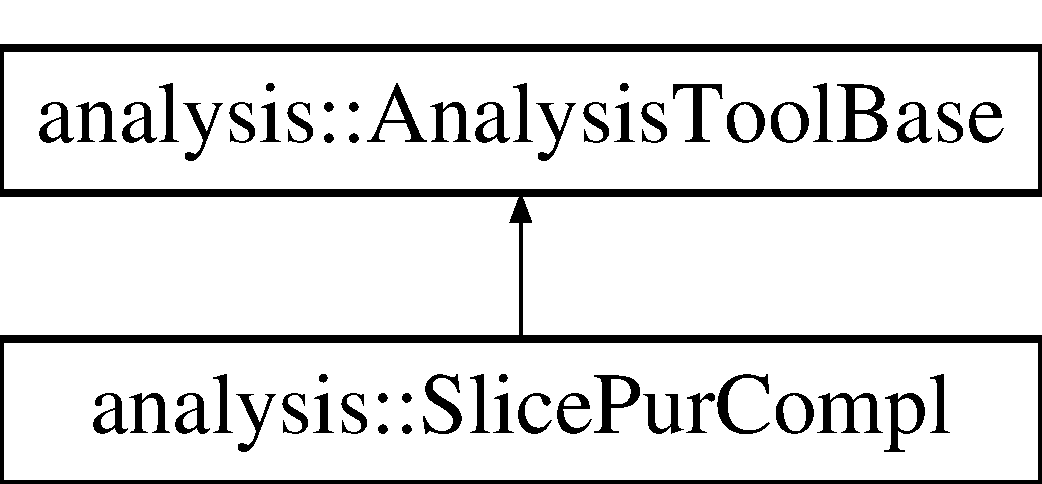
\includegraphics[height=2.000000cm]{classanalysis_1_1SlicePurCompl}
\end{center}
\end{figure}
\subsection*{Public Member Functions}
\begin{DoxyCompactItemize}
\item 
\hyperlink{classanalysis_1_1SlicePurCompl_a8d0b7176feea1c0cda563f1a528a4643}{Slice\-Pur\-Compl} (const fhicl\-::\-Parameter\-Set \&pset)
\begin{DoxyCompactList}\small\item\em Constructor. \end{DoxyCompactList}\item 
\hypertarget{classanalysis_1_1SlicePurCompl_aba1c519efb59ad152d186ab4a1a2c6ca}{\hyperlink{classanalysis_1_1SlicePurCompl_aba1c519efb59ad152d186ab4a1a2c6ca}{$\sim$\-Slice\-Pur\-Compl} ()}\label{classanalysis_1_1SlicePurCompl_aba1c519efb59ad152d186ab4a1a2c6ca}

\begin{DoxyCompactList}\small\item\em Destructor. \end{DoxyCompactList}\item 
void \hyperlink{classanalysis_1_1SlicePurCompl_a902e57f96d7a335793856af6c7f7580f}{configure} (fhicl\-::\-Parameter\-Set const \&pset)
\item 
void \hyperlink{classanalysis_1_1SlicePurCompl_af71528c37c501d30f5bbc1e75b50b3f6}{analyze\-Event} (art\-::\-Event const \&e, bool f\-Data) override
\begin{DoxyCompactList}\small\item\em Analysis function. \end{DoxyCompactList}\item 
\hypertarget{classanalysis_1_1SlicePurCompl_ab13316464f9ed61e81b18d59ca38d9a1}{void \hyperlink{classanalysis_1_1SlicePurCompl_ab13316464f9ed61e81b18d59ca38d9a1}{analyze\-Slice} (art\-::\-Event const \&e, std\-::vector$<$ Proxy\-Pfp\-Elem\-\_\-t $>$ \&slice\-\_\-pfp\-\_\-v, bool f\-Data, bool selected) override}\label{classanalysis_1_1SlicePurCompl_ab13316464f9ed61e81b18d59ca38d9a1}

\begin{DoxyCompactList}\small\item\em Analyze slice. \end{DoxyCompactList}\item 
\hypertarget{classanalysis_1_1SlicePurCompl_a39079f2f29d253440c7ebd2deeaccfef}{void \hyperlink{classanalysis_1_1SlicePurCompl_a39079f2f29d253440c7ebd2deeaccfef}{Save\-Truth} (art\-::\-Event const \&e)}\label{classanalysis_1_1SlicePurCompl_a39079f2f29d253440c7ebd2deeaccfef}

\begin{DoxyCompactList}\small\item\em Save truth info for event associated to neutrino. \end{DoxyCompactList}\item 
\hypertarget{classanalysis_1_1SlicePurCompl_ae7e1131785f819a530a573c6b20d1cbc}{void \hyperlink{classanalysis_1_1SlicePurCompl_ae7e1131785f819a530a573c6b20d1cbc}{set\-Branches} (T\-Tree $\ast$\-\_\-tree) override}\label{classanalysis_1_1SlicePurCompl_ae7e1131785f819a530a573c6b20d1cbc}

\begin{DoxyCompactList}\small\item\em set branches for T\-Tree \end{DoxyCompactList}\item 
\hypertarget{classanalysis_1_1SlicePurCompl_a43bf5b44e619f2dc3e5d00098048471b}{void \hyperlink{classanalysis_1_1SlicePurCompl_a43bf5b44e619f2dc3e5d00098048471b}{reset\-T\-Tree} (T\-Tree $\ast$\-\_\-tree) override}\label{classanalysis_1_1SlicePurCompl_a43bf5b44e619f2dc3e5d00098048471b}

\begin{DoxyCompactList}\small\item\em reset ttree branches \end{DoxyCompactList}\end{DoxyCompactItemize}
\subsection*{Private Member Functions}
\begin{DoxyCompactItemize}
\item 
\hypertarget{classanalysis_1_1SlicePurCompl_a1cab4a3ebdd3aae05b22ad5d06a6ce1b}{void {\bfseries fill\-Id} (const std\-::vector$<$ double $>$ \&p, const simb\-::\-M\-C\-Particle \&mcp, std\-::vector$<$ size\-\_\-t $>$ \&id)}\label{classanalysis_1_1SlicePurCompl_a1cab4a3ebdd3aae05b22ad5d06a6ce1b}

\item 
\hypertarget{classanalysis_1_1SlicePurCompl_a3ae6a4a95f5d387edd47f3646bc39c70}{void {\bfseries increment\-Counts} (const std\-::vector$<$ art\-::\-Ptr$<$ recob\-::\-Hit $>$ $>$ \&hits, const std\-::unique\-\_\-ptr$<$ art\-::\-Find\-Many\-P$<$ simb\-::\-M\-C\-Particle, anab\-::\-Back\-Tracker\-Hit\-Matching\-Data $>$ $>$ \&assoc\-M\-C\-Part, const std\-::vector$<$ size\-\_\-t $>$ \&lepid, const std\-::vector$<$ size\-\_\-t $>$ \&proid, const std\-::vector$<$ size\-\_\-t $>$ \&pi1id, const std\-::vector$<$ size\-\_\-t $>$ \&pi0id, const std\-::vector$<$ size\-\_\-t $>$ \&neuid, const std\-::vector$<$ size\-\_\-t $>$ \&gamid, const std\-::vector$<$ size\-\_\-t $>$ \&othid, int \&nlephits, int \&nprohits, int \&npi1hits, int \&npi0hits, int \&nneuhits, int \&ngamhits, int \&nothhits) const }\label{classanalysis_1_1SlicePurCompl_a3ae6a4a95f5d387edd47f3646bc39c70}

\end{DoxyCompactItemize}
\subsection*{Private Attributes}
\begin{DoxyCompactItemize}
\item 
\hypertarget{classanalysis_1_1SlicePurCompl_a307c2d9ddcce991a9d96dd3a2671fc3b}{art\-::\-Input\-Tag {\bfseries f\-C\-L\-Sproducer}}\label{classanalysis_1_1SlicePurCompl_a307c2d9ddcce991a9d96dd3a2671fc3b}

\item 
\hypertarget{classanalysis_1_1SlicePurCompl_a3df191801ef5aac0aedb5adcd820c250}{art\-::\-Input\-Tag {\bfseries f\-S\-L\-Cproducer}}\label{classanalysis_1_1SlicePurCompl_a3df191801ef5aac0aedb5adcd820c250}

\item 
\hypertarget{classanalysis_1_1SlicePurCompl_ae71cdd3989046e48d2251aa373ecfa98}{art\-::\-Input\-Tag {\bfseries f\-M\-C\-Tproducer}}\label{classanalysis_1_1SlicePurCompl_ae71cdd3989046e48d2251aa373ecfa98}

\item 
\hypertarget{classanalysis_1_1SlicePurCompl_a6b925d0776a50667c224a8e74922d845}{art\-::\-Input\-Tag {\bfseries f\-M\-C\-Pproducer}}\label{classanalysis_1_1SlicePurCompl_a6b925d0776a50667c224a8e74922d845}

\item 
\hypertarget{classanalysis_1_1SlicePurCompl_ac9a3b16af45681b89a5899fedc01696a}{art\-::\-Input\-Tag {\bfseries f\-Hproducer}}\label{classanalysis_1_1SlicePurCompl_ac9a3b16af45681b89a5899fedc01696a}

\item 
\hypertarget{classanalysis_1_1SlicePurCompl_a0f80f3d333ae1c52518f0a364afd4647}{art\-::\-Input\-Tag {\bfseries f\-H\-Tproducer}}\label{classanalysis_1_1SlicePurCompl_a0f80f3d333ae1c52518f0a364afd4647}

\item 
\hypertarget{classanalysis_1_1SlicePurCompl_ad45bcb68994499cd6582911929ba617e}{std\-::vector$<$ size\-\_\-t $>$ {\bfseries lepid}}\label{classanalysis_1_1SlicePurCompl_ad45bcb68994499cd6582911929ba617e}

\item 
\hypertarget{classanalysis_1_1SlicePurCompl_a43aab4b627345ae1059d838eaf05322d}{std\-::vector$<$ size\-\_\-t $>$ {\bfseries proid}}\label{classanalysis_1_1SlicePurCompl_a43aab4b627345ae1059d838eaf05322d}

\item 
\hypertarget{classanalysis_1_1SlicePurCompl_a70db8876abcc7434d813d235acac332c}{std\-::vector$<$ size\-\_\-t $>$ {\bfseries pi1id}}\label{classanalysis_1_1SlicePurCompl_a70db8876abcc7434d813d235acac332c}

\item 
\hypertarget{classanalysis_1_1SlicePurCompl_aaa4d7b9339cb5e7e1b2abce6b4784532}{std\-::vector$<$ size\-\_\-t $>$ {\bfseries pi0id}}\label{classanalysis_1_1SlicePurCompl_aaa4d7b9339cb5e7e1b2abce6b4784532}

\item 
\hypertarget{classanalysis_1_1SlicePurCompl_a1f6b97343b50a45f6d08c9b7a77cafc8}{std\-::vector$<$ size\-\_\-t $>$ {\bfseries neuid}}\label{classanalysis_1_1SlicePurCompl_a1f6b97343b50a45f6d08c9b7a77cafc8}

\item 
\hypertarget{classanalysis_1_1SlicePurCompl_a4123f24a7b7c48a0b8d035d8f6cd8855}{std\-::vector$<$ size\-\_\-t $>$ {\bfseries gamid}}\label{classanalysis_1_1SlicePurCompl_a4123f24a7b7c48a0b8d035d8f6cd8855}

\item 
\hypertarget{classanalysis_1_1SlicePurCompl_ab09dc6647525b89ebee6e9ee622cce58}{std\-::vector$<$ size\-\_\-t $>$ {\bfseries othid}}\label{classanalysis_1_1SlicePurCompl_ab09dc6647525b89ebee6e9ee622cce58}

\item 
\hypertarget{classanalysis_1_1SlicePurCompl_aee3dce7966b5e1ea71c93413bcbc6d8a}{std\-::unique\-\_\-ptr\\*
$<$ art\-::\-Find\-Many\-P\\*
$<$ simb\-::\-M\-C\-Particle, \\*
anab\-::\-Back\-Tracker\-Hit\-Matching\-Data $>$ $>$ {\bfseries assoc\-M\-C\-Part}}\label{classanalysis_1_1SlicePurCompl_aee3dce7966b5e1ea71c93413bcbc6d8a}

\item 
\hypertarget{classanalysis_1_1SlicePurCompl_abb4d90c2bccf98be8583ee7ec4786e7b}{int {\bfseries evnunhits}}\label{classanalysis_1_1SlicePurCompl_abb4d90c2bccf98be8583ee7ec4786e7b}

\item 
\hypertarget{classanalysis_1_1SlicePurCompl_acb6c47c5f5079404267f46ad6ccd843e}{int {\bfseries evlepnhits}}\label{classanalysis_1_1SlicePurCompl_acb6c47c5f5079404267f46ad6ccd843e}

\item 
\hypertarget{classanalysis_1_1SlicePurCompl_a3b7e6beaede5fdaab4b4d58e3702fea1}{int {\bfseries evpronhits}}\label{classanalysis_1_1SlicePurCompl_a3b7e6beaede5fdaab4b4d58e3702fea1}

\item 
\hypertarget{classanalysis_1_1SlicePurCompl_a2b450063c61b0408260de63628f3d544}{int {\bfseries evpi1nhits}}\label{classanalysis_1_1SlicePurCompl_a2b450063c61b0408260de63628f3d544}

\item 
\hypertarget{classanalysis_1_1SlicePurCompl_a09f10f4336fd100d37288c28aa760d6c}{int {\bfseries evpi0nhits}}\label{classanalysis_1_1SlicePurCompl_a09f10f4336fd100d37288c28aa760d6c}

\item 
\hypertarget{classanalysis_1_1SlicePurCompl_ab2c486fe3cd267b02bfe43287e0292cc}{int {\bfseries evneunhits}}\label{classanalysis_1_1SlicePurCompl_ab2c486fe3cd267b02bfe43287e0292cc}

\item 
\hypertarget{classanalysis_1_1SlicePurCompl_a7e73b2e419ef876d6eb5461cb0f545e8}{int {\bfseries evgamnhits}}\label{classanalysis_1_1SlicePurCompl_a7e73b2e419ef876d6eb5461cb0f545e8}

\item 
\hypertarget{classanalysis_1_1SlicePurCompl_a4ffaa86db84a7b653e5cb9d46a438ad6}{int {\bfseries evothnhits}}\label{classanalysis_1_1SlicePurCompl_a4ffaa86db84a7b653e5cb9d46a438ad6}

\item 
\hypertarget{classanalysis_1_1SlicePurCompl_af47aa616a06d9b8d3faa339d84ae4438}{int {\bfseries slnunhits}}\label{classanalysis_1_1SlicePurCompl_af47aa616a06d9b8d3faa339d84ae4438}

\item 
\hypertarget{classanalysis_1_1SlicePurCompl_add1eb3fea3a112c87148a2ae1b8277c3}{int {\bfseries sllepnhits}}\label{classanalysis_1_1SlicePurCompl_add1eb3fea3a112c87148a2ae1b8277c3}

\item 
\hypertarget{classanalysis_1_1SlicePurCompl_a61e069054e22a820fb8dc7d66256a910}{int {\bfseries slpronhits}}\label{classanalysis_1_1SlicePurCompl_a61e069054e22a820fb8dc7d66256a910}

\item 
\hypertarget{classanalysis_1_1SlicePurCompl_a50a372d72b26c4d5a9a9ade5f2f5eab2}{int {\bfseries slpi1nhits}}\label{classanalysis_1_1SlicePurCompl_a50a372d72b26c4d5a9a9ade5f2f5eab2}

\item 
\hypertarget{classanalysis_1_1SlicePurCompl_ad703a2ae2ce73fbd89da4a70d3580528}{int {\bfseries slpi0nhits}}\label{classanalysis_1_1SlicePurCompl_ad703a2ae2ce73fbd89da4a70d3580528}

\item 
\hypertarget{classanalysis_1_1SlicePurCompl_a19d1e785c35c38700153641be818f294}{int {\bfseries slneunhits}}\label{classanalysis_1_1SlicePurCompl_a19d1e785c35c38700153641be818f294}

\item 
\hypertarget{classanalysis_1_1SlicePurCompl_a60ead841a2465f1988407ce2acabc127}{int {\bfseries slgamnhits}}\label{classanalysis_1_1SlicePurCompl_a60ead841a2465f1988407ce2acabc127}

\item 
\hypertarget{classanalysis_1_1SlicePurCompl_a91211d43ef13153108fe8c5890959e41}{int {\bfseries slothnhits}}\label{classanalysis_1_1SlicePurCompl_a91211d43ef13153108fe8c5890959e41}

\item 
\hypertarget{classanalysis_1_1SlicePurCompl_a1110efa7e03c55c097074dfaff97cc76}{std\-::vector$<$ int $>$ {\bfseries pfnunhits}}\label{classanalysis_1_1SlicePurCompl_a1110efa7e03c55c097074dfaff97cc76}

\item 
\hypertarget{classanalysis_1_1SlicePurCompl_ac95a09b13737e44d4fd2c3290f697789}{std\-::vector$<$ int $>$ {\bfseries pflepnhits}}\label{classanalysis_1_1SlicePurCompl_ac95a09b13737e44d4fd2c3290f697789}

\item 
\hypertarget{classanalysis_1_1SlicePurCompl_a897ea8a7d8edad962708cd07e81e4027}{std\-::vector$<$ int $>$ {\bfseries pfpronhits}}\label{classanalysis_1_1SlicePurCompl_a897ea8a7d8edad962708cd07e81e4027}

\item 
\hypertarget{classanalysis_1_1SlicePurCompl_ac139f48479667236bead6aaac1832285}{std\-::vector$<$ int $>$ {\bfseries pfpi1nhits}}\label{classanalysis_1_1SlicePurCompl_ac139f48479667236bead6aaac1832285}

\item 
\hypertarget{classanalysis_1_1SlicePurCompl_a7d1e165214a285fd67d5f46690888716}{std\-::vector$<$ int $>$ {\bfseries pfpi0nhits}}\label{classanalysis_1_1SlicePurCompl_a7d1e165214a285fd67d5f46690888716}

\item 
\hypertarget{classanalysis_1_1SlicePurCompl_a076e4b38d7fdc869f72bf783ea425e1c}{std\-::vector$<$ int $>$ {\bfseries pfneunhits}}\label{classanalysis_1_1SlicePurCompl_a076e4b38d7fdc869f72bf783ea425e1c}

\item 
\hypertarget{classanalysis_1_1SlicePurCompl_a1ebbad4d92fab6cc0383b7c378350f6b}{std\-::vector$<$ int $>$ {\bfseries pfgamnhits}}\label{classanalysis_1_1SlicePurCompl_a1ebbad4d92fab6cc0383b7c378350f6b}

\item 
\hypertarget{classanalysis_1_1SlicePurCompl_a2925bdf47da943b053693527fbbca375}{std\-::vector$<$ int $>$ {\bfseries pfothnhits}}\label{classanalysis_1_1SlicePurCompl_a2925bdf47da943b053693527fbbca375}

\end{DoxyCompactItemize}


\subsection{Constructor \& Destructor Documentation}
\hypertarget{classanalysis_1_1SlicePurCompl_a8d0b7176feea1c0cda563f1a528a4643}{\index{analysis\-::\-Slice\-Pur\-Compl@{analysis\-::\-Slice\-Pur\-Compl}!Slice\-Pur\-Compl@{Slice\-Pur\-Compl}}
\index{Slice\-Pur\-Compl@{Slice\-Pur\-Compl}!analysis::SlicePurCompl@{analysis\-::\-Slice\-Pur\-Compl}}
\subsubsection[{Slice\-Pur\-Compl}]{\setlength{\rightskip}{0pt plus 5cm}analysis\-::\-Slice\-Pur\-Compl\-::\-Slice\-Pur\-Compl (
\begin{DoxyParamCaption}
\item[{const fhicl\-::\-Parameter\-Set \&}]{p}
\end{DoxyParamCaption}
)}}\label{classanalysis_1_1SlicePurCompl_a8d0b7176feea1c0cda563f1a528a4643}


Constructor. 


\begin{DoxyParams}{Parameters}
{\em pset} & Constructor.\\
\hline
\end{DoxyParams}
Arguments\-:

pset -\/ Fcl parameters. 

\subsection{Member Function Documentation}
\hypertarget{classanalysis_1_1SlicePurCompl_af71528c37c501d30f5bbc1e75b50b3f6}{\index{analysis\-::\-Slice\-Pur\-Compl@{analysis\-::\-Slice\-Pur\-Compl}!analyze\-Event@{analyze\-Event}}
\index{analyze\-Event@{analyze\-Event}!analysis::SlicePurCompl@{analysis\-::\-Slice\-Pur\-Compl}}
\subsubsection[{analyze\-Event}]{\setlength{\rightskip}{0pt plus 5cm}void analysis\-::\-Slice\-Pur\-Compl\-::analyze\-Event (
\begin{DoxyParamCaption}
\item[{art\-::\-Event const \&}]{e, }
\item[{bool}]{f\-Data}
\end{DoxyParamCaption}
)\hspace{0.3cm}{\ttfamily [override]}, {\ttfamily [virtual]}}}\label{classanalysis_1_1SlicePurCompl_af71528c37c501d30f5bbc1e75b50b3f6}


Analysis function. 

Reconfigure method.

Arguments\-:

pset -\/ Fcl parameter set. 

Implements \hyperlink{classanalysis_1_1AnalysisToolBase_ad5079f85c78e6c40f70ebf4ee31f5600}{analysis\-::\-Analysis\-Tool\-Base}.

\hypertarget{classanalysis_1_1SlicePurCompl_a902e57f96d7a335793856af6c7f7580f}{\index{analysis\-::\-Slice\-Pur\-Compl@{analysis\-::\-Slice\-Pur\-Compl}!configure@{configure}}
\index{configure@{configure}!analysis::SlicePurCompl@{analysis\-::\-Slice\-Pur\-Compl}}
\subsubsection[{configure}]{\setlength{\rightskip}{0pt plus 5cm}void analysis\-::\-Slice\-Pur\-Compl\-::configure (
\begin{DoxyParamCaption}
\item[{fhicl\-::\-Parameter\-Set const \&}]{p}
\end{DoxyParamCaption}
)}}\label{classanalysis_1_1SlicePurCompl_a902e57f96d7a335793856af6c7f7580f}
Reconfigure method.

Arguments\-:

pset -\/ Fcl parameter set. 

The documentation for this class was generated from the following file\-:\begin{DoxyCompactItemize}
\item 
/home/travis/build/ubneutrinos/searchingfornues/\-Selection/\-Analysis\-Tools/Slice\-Pur\-Compl\-\_\-tool.\-cc\end{DoxyCompactItemize}

\hypertarget{classanalysis_1_1TrackAnalysis}{}\section{analysis\+:\+:Track\+Analysis Class Reference}
\label{classanalysis_1_1TrackAnalysis}\index{analysis\+::\+Track\+Analysis@{analysis\+::\+Track\+Analysis}}
Inheritance diagram for analysis\+:\+:Track\+Analysis\+:\begin{figure}[H]
\begin{center}
\leavevmode
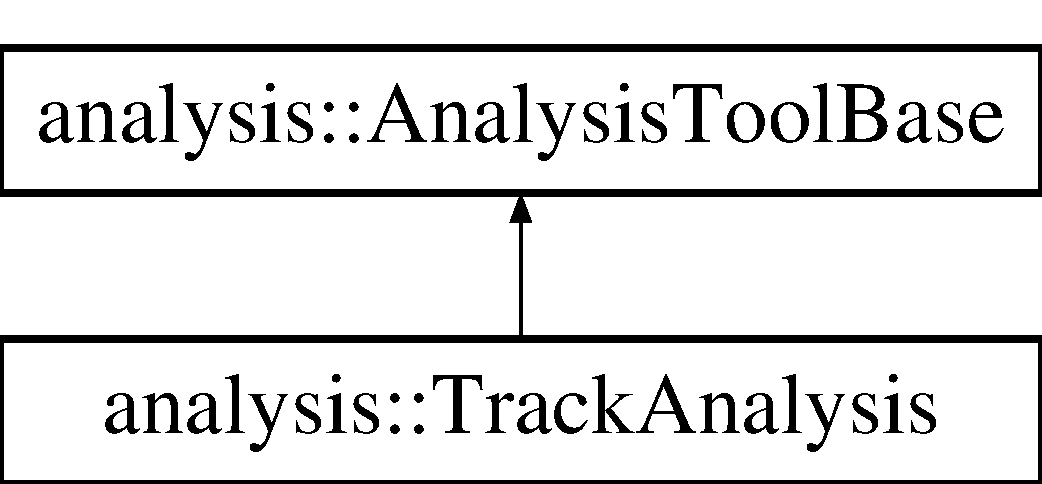
\includegraphics[height=2.000000cm]{classanalysis_1_1TrackAnalysis}
\end{center}
\end{figure}
\subsection*{Public Member Functions}
\begin{DoxyCompactItemize}
\item 
\hyperlink{classanalysis_1_1TrackAnalysis_aed13157ba9297149fe4e15676e6db7fc}{Track\+Analysis} (const fhicl\+::\+Parameter\+Set \&pset)
\begin{DoxyCompactList}\small\item\em Constructor. \end{DoxyCompactList}\item 
\hyperlink{classanalysis_1_1TrackAnalysis_a6f96bc87ab6d9dffb6417d7d2f1a89e2}{$\sim$\+Track\+Analysis} ()\hypertarget{classanalysis_1_1TrackAnalysis_a6f96bc87ab6d9dffb6417d7d2f1a89e2}{}\label{classanalysis_1_1TrackAnalysis_a6f96bc87ab6d9dffb6417d7d2f1a89e2}

\begin{DoxyCompactList}\small\item\em Destructor. \end{DoxyCompactList}\item 
void \hyperlink{classanalysis_1_1TrackAnalysis_a427d588370a8044b77560c92d3a35ea6}{configure} (fhicl\+::\+Parameter\+Set const \&pset)
\item 
void \hyperlink{classanalysis_1_1TrackAnalysis_aa5a295fc3fe8aa050905361f469ff108}{analyze\+Event} (art\+::\+Event const \&e, bool f\+Data) override
\begin{DoxyCompactList}\small\item\em Analysis function. \end{DoxyCompactList}\item 
void \hyperlink{classanalysis_1_1TrackAnalysis_a00e51059eed5a6486c9eb2f2f16017de}{analyze\+Slice} (art\+::\+Event const \&e, std\+::vector$<$ Proxy\+Pfp\+Elem\+\_\+t $>$ \&slice\+\_\+pfp\+\_\+v, bool f\+Data, bool selected) override\hypertarget{classanalysis_1_1TrackAnalysis_a00e51059eed5a6486c9eb2f2f16017de}{}\label{classanalysis_1_1TrackAnalysis_a00e51059eed5a6486c9eb2f2f16017de}

\begin{DoxyCompactList}\small\item\em Analyze slice. \end{DoxyCompactList}\item 
void \hyperlink{classanalysis_1_1TrackAnalysis_adde7746b5a45ec99cd67c0ab1fa19eb1}{Save\+Truth} (art\+::\+Event const \&e)\hypertarget{classanalysis_1_1TrackAnalysis_adde7746b5a45ec99cd67c0ab1fa19eb1}{}\label{classanalysis_1_1TrackAnalysis_adde7746b5a45ec99cd67c0ab1fa19eb1}

\begin{DoxyCompactList}\small\item\em Save truth info for event associated to neutrino. \end{DoxyCompactList}\item 
void \hyperlink{classanalysis_1_1TrackAnalysis_ace1af1d0be520c1319758a9391f5bc4d}{fill\+Default} ()\hypertarget{classanalysis_1_1TrackAnalysis_ace1af1d0be520c1319758a9391f5bc4d}{}\label{classanalysis_1_1TrackAnalysis_ace1af1d0be520c1319758a9391f5bc4d}

\begin{DoxyCompactList}\small\item\em Fill Default info for event associated to neutrino. \end{DoxyCompactList}\item 
void \hyperlink{classanalysis_1_1TrackAnalysis_ae89023f1c4b11cae7bb4acb672006bb7}{set\+Branches} (T\+Tree $\ast$\+\_\+tree) override\hypertarget{classanalysis_1_1TrackAnalysis_ae89023f1c4b11cae7bb4acb672006bb7}{}\label{classanalysis_1_1TrackAnalysis_ae89023f1c4b11cae7bb4acb672006bb7}

\begin{DoxyCompactList}\small\item\em set branches for T\+Tree \end{DoxyCompactList}\item 
void \hyperlink{classanalysis_1_1TrackAnalysis_a088a56418549d45b22df10270068caca}{reset\+T\+Tree} (T\+Tree $\ast$\+\_\+tree) override\hypertarget{classanalysis_1_1TrackAnalysis_a088a56418549d45b22df10270068caca}{}\label{classanalysis_1_1TrackAnalysis_a088a56418549d45b22df10270068caca}

\begin{DoxyCompactList}\small\item\em reset ttree branches \end{DoxyCompactList}\end{DoxyCompactItemize}
\subsection*{Private Attributes}
\begin{DoxyCompactItemize}
\item 
const trkf\+::\+Track\+Momentum\+Calculator {\bfseries \+\_\+trkmom}\hypertarget{classanalysis_1_1TrackAnalysis_a22599de9de269967cfdfb8490fcc3897}{}\label{classanalysis_1_1TrackAnalysis_a22599de9de269967cfdfb8490fcc3897}

\item 
const trkf\+::\+Trajectory\+M\+C\+S\+Fitter {\bfseries \+\_\+mcsfitter}\hypertarget{classanalysis_1_1TrackAnalysis_a97631d64480702a4b7589a5bb9d735aa}{}\label{classanalysis_1_1TrackAnalysis_a97631d64480702a4b7589a5bb9d735aa}

\item 
T\+Particle\+P\+DG $\ast$ {\bfseries proton} = T\+Database\+P\+D\+G\+::\+Instance()-\/$>$Get\+Particle(2212)\hypertarget{classanalysis_1_1TrackAnalysis_a4adc7f89c334ab93747a8d4c4abbcc6d}{}\label{classanalysis_1_1TrackAnalysis_a4adc7f89c334ab93747a8d4c4abbcc6d}

\item 
T\+Particle\+P\+DG $\ast$ {\bfseries muon} = T\+Database\+P\+D\+G\+::\+Instance()-\/$>$Get\+Particle(13)\hypertarget{classanalysis_1_1TrackAnalysis_a0fe3b9e7864aaaa36b5f52826b4e3eb9}{}\label{classanalysis_1_1TrackAnalysis_a0fe3b9e7864aaaa36b5f52826b4e3eb9}

\item 
\hyperlink{classsearchingfornues_1_1LLRPID}{searchingfornues\+::\+L\+L\+R\+P\+ID} {\bfseries llr\+\_\+pid\+\_\+calculator}\hypertarget{classanalysis_1_1TrackAnalysis_a9aa071870faf165eb6548f0ea16e4132}{}\label{classanalysis_1_1TrackAnalysis_a9aa071870faf165eb6548f0ea16e4132}

\item 
art\+::\+Input\+Tag {\bfseries f\+C\+A\+L\+Oproducer}\hypertarget{classanalysis_1_1TrackAnalysis_a0ceaf940b041eda0237cc73cd330d18d}{}\label{classanalysis_1_1TrackAnalysis_a0ceaf940b041eda0237cc73cd330d18d}

\item 
art\+::\+Input\+Tag {\bfseries f\+P\+I\+Dproducer}\hypertarget{classanalysis_1_1TrackAnalysis_a349dc117e508190c619cd9f47ea7647e}{}\label{classanalysis_1_1TrackAnalysis_a349dc117e508190c619cd9f47ea7647e}

\item 
art\+::\+Input\+Tag {\bfseries f\+T\+R\+Kproducer}\hypertarget{classanalysis_1_1TrackAnalysis_a45abdcf3140e68a2ce90501e33a00eb3}{}\label{classanalysis_1_1TrackAnalysis_a45abdcf3140e68a2ce90501e33a00eb3}

\item 
art\+::\+Input\+Tag {\bfseries f\+Backtrack\+Tag}\hypertarget{classanalysis_1_1TrackAnalysis_ac8e03baef9070b09d0a6e266928f8b18}{}\label{classanalysis_1_1TrackAnalysis_ac8e03baef9070b09d0a6e266928f8b18}

\item 
art\+::\+Input\+Tag {\bfseries f\+Hproducer}\hypertarget{classanalysis_1_1TrackAnalysis_a44ff6c3a2361b97c9c7f4faf466a86ad}{}\label{classanalysis_1_1TrackAnalysis_a44ff6c3a2361b97c9c7f4faf466a86ad}

\item 
bool {\bfseries f\+Recalibrate\+Hits}\hypertarget{classanalysis_1_1TrackAnalysis_aaf18243d05cd2a068268a03a5ab39c66}{}\label{classanalysis_1_1TrackAnalysis_aaf18243d05cd2a068268a03a5ab39c66}

\item 
float {\bfseries f\+Energy\+Threshold\+For\+M\+C\+Hits}\hypertarget{classanalysis_1_1TrackAnalysis_a85055289f4326f2cfb9d6957c2156d6a}{}\label{classanalysis_1_1TrackAnalysis_a85055289f4326f2cfb9d6957c2156d6a}

\item 
int {\bfseries \+\_\+run}\hypertarget{classanalysis_1_1TrackAnalysis_aa9a9d585543f931ac8b736f39a7dc4a5}{}\label{classanalysis_1_1TrackAnalysis_aa9a9d585543f931ac8b736f39a7dc4a5}

\item 
int {\bfseries \+\_\+sub}\hypertarget{classanalysis_1_1TrackAnalysis_ab85c46d9a61e56c9390814196ac18ab6}{}\label{classanalysis_1_1TrackAnalysis_ab85c46d9a61e56c9390814196ac18ab6}

\item 
int {\bfseries \+\_\+evt}\hypertarget{classanalysis_1_1TrackAnalysis_a1aa922e8130e193a434a4291f1b67d2f}{}\label{classanalysis_1_1TrackAnalysis_a1aa922e8130e193a434a4291f1b67d2f}

\item 
std\+::vector$<$ size\+\_\+t $>$ {\bfseries \+\_\+trk\+\_\+pfp\+\_\+id\+\_\+v}\hypertarget{classanalysis_1_1TrackAnalysis_a204ef1a35c4346e36ffba8ced3c6ce5c}{}\label{classanalysis_1_1TrackAnalysis_a204ef1a35c4346e36ffba8ced3c6ce5c}

\item 
std\+::vector$<$ float $>$ {\bfseries \+\_\+trk\+\_\+start\+\_\+x\+\_\+v}\hypertarget{classanalysis_1_1TrackAnalysis_a221179d7babe341c075f5efd23816131}{}\label{classanalysis_1_1TrackAnalysis_a221179d7babe341c075f5efd23816131}

\item 
std\+::vector$<$ float $>$ {\bfseries \+\_\+trk\+\_\+start\+\_\+y\+\_\+v}\hypertarget{classanalysis_1_1TrackAnalysis_a22a1126cccb5cb0a17bfb1406678cf69}{}\label{classanalysis_1_1TrackAnalysis_a22a1126cccb5cb0a17bfb1406678cf69}

\item 
std\+::vector$<$ float $>$ {\bfseries \+\_\+trk\+\_\+start\+\_\+z\+\_\+v}\hypertarget{classanalysis_1_1TrackAnalysis_a546c29bebe8ce807b1a0abdcbb87f252}{}\label{classanalysis_1_1TrackAnalysis_a546c29bebe8ce807b1a0abdcbb87f252}

\item 
std\+::vector$<$ float $>$ {\bfseries \+\_\+trk\+\_\+sce\+\_\+start\+\_\+x\+\_\+v}\hypertarget{classanalysis_1_1TrackAnalysis_a94cfdc8ed703a9f7ba24940e2d67f4f5}{}\label{classanalysis_1_1TrackAnalysis_a94cfdc8ed703a9f7ba24940e2d67f4f5}

\item 
std\+::vector$<$ float $>$ {\bfseries \+\_\+trk\+\_\+sce\+\_\+start\+\_\+y\+\_\+v}\hypertarget{classanalysis_1_1TrackAnalysis_a8fe34d43546083dcbe242318d35e057d}{}\label{classanalysis_1_1TrackAnalysis_a8fe34d43546083dcbe242318d35e057d}

\item 
std\+::vector$<$ float $>$ {\bfseries \+\_\+trk\+\_\+sce\+\_\+start\+\_\+z\+\_\+v}\hypertarget{classanalysis_1_1TrackAnalysis_ac40437eb94d4df9d9fab95ffff6678f9}{}\label{classanalysis_1_1TrackAnalysis_ac40437eb94d4df9d9fab95ffff6678f9}

\item 
std\+::vector$<$ float $>$ {\bfseries \+\_\+trk\+\_\+distance\+\_\+v}\hypertarget{classanalysis_1_1TrackAnalysis_a3d193e8d67655448962d3f3f9b5bc8dd}{}\label{classanalysis_1_1TrackAnalysis_a3d193e8d67655448962d3f3f9b5bc8dd}

\item 
std\+::vector$<$ float $>$ {\bfseries \+\_\+trk\+\_\+theta\+\_\+v}\hypertarget{classanalysis_1_1TrackAnalysis_add6ab02f075045913b33ee4a566eb078}{}\label{classanalysis_1_1TrackAnalysis_add6ab02f075045913b33ee4a566eb078}

\item 
std\+::vector$<$ float $>$ {\bfseries \+\_\+trk\+\_\+phi\+\_\+v}\hypertarget{classanalysis_1_1TrackAnalysis_a478f0e5341895c4d23557f6803fc5a9b}{}\label{classanalysis_1_1TrackAnalysis_a478f0e5341895c4d23557f6803fc5a9b}

\item 
std\+::vector$<$ float $>$ {\bfseries \+\_\+trk\+\_\+dir\+\_\+x\+\_\+v}\hypertarget{classanalysis_1_1TrackAnalysis_af92fafa75f438f5d5ffc5c30e39438ad}{}\label{classanalysis_1_1TrackAnalysis_af92fafa75f438f5d5ffc5c30e39438ad}

\item 
std\+::vector$<$ float $>$ {\bfseries \+\_\+trk\+\_\+dir\+\_\+y\+\_\+v}\hypertarget{classanalysis_1_1TrackAnalysis_a41be71127f4637eb8649e49720e16554}{}\label{classanalysis_1_1TrackAnalysis_a41be71127f4637eb8649e49720e16554}

\item 
std\+::vector$<$ float $>$ {\bfseries \+\_\+trk\+\_\+dir\+\_\+z\+\_\+v}\hypertarget{classanalysis_1_1TrackAnalysis_af560ca963a50e03894414a8b2b04ae18}{}\label{classanalysis_1_1TrackAnalysis_af560ca963a50e03894414a8b2b04ae18}

\item 
std\+::vector$<$ float $>$ {\bfseries \+\_\+trk\+\_\+end\+\_\+x\+\_\+v}\hypertarget{classanalysis_1_1TrackAnalysis_a0978b4d1abaa1216cfd627ccd88ec3e8}{}\label{classanalysis_1_1TrackAnalysis_a0978b4d1abaa1216cfd627ccd88ec3e8}

\item 
std\+::vector$<$ float $>$ {\bfseries \+\_\+trk\+\_\+end\+\_\+y\+\_\+v}\hypertarget{classanalysis_1_1TrackAnalysis_a395bd060dbdafb908ab4c4349e11ce94}{}\label{classanalysis_1_1TrackAnalysis_a395bd060dbdafb908ab4c4349e11ce94}

\item 
std\+::vector$<$ float $>$ {\bfseries \+\_\+trk\+\_\+end\+\_\+z\+\_\+v}\hypertarget{classanalysis_1_1TrackAnalysis_a3709728bbb087fac8b08037c5ca3f2c9}{}\label{classanalysis_1_1TrackAnalysis_a3709728bbb087fac8b08037c5ca3f2c9}

\item 
std\+::vector$<$ float $>$ {\bfseries \+\_\+trk\+\_\+sce\+\_\+end\+\_\+x\+\_\+v}\hypertarget{classanalysis_1_1TrackAnalysis_a945f236cab0698ad2eff2b81841d4699}{}\label{classanalysis_1_1TrackAnalysis_a945f236cab0698ad2eff2b81841d4699}

\item 
std\+::vector$<$ float $>$ {\bfseries \+\_\+trk\+\_\+sce\+\_\+end\+\_\+y\+\_\+v}\hypertarget{classanalysis_1_1TrackAnalysis_ae5202ef05a836b9a51de3e34ea7045e3}{}\label{classanalysis_1_1TrackAnalysis_ae5202ef05a836b9a51de3e34ea7045e3}

\item 
std\+::vector$<$ float $>$ {\bfseries \+\_\+trk\+\_\+sce\+\_\+end\+\_\+z\+\_\+v}\hypertarget{classanalysis_1_1TrackAnalysis_ae61a54d9550fdcc47db7d78072ec140b}{}\label{classanalysis_1_1TrackAnalysis_ae61a54d9550fdcc47db7d78072ec140b}

\item 
std\+::vector$<$ float $>$ {\bfseries \+\_\+trk\+\_\+len\+\_\+v}\hypertarget{classanalysis_1_1TrackAnalysis_a68a26309363978c671172515e67213d4}{}\label{classanalysis_1_1TrackAnalysis_a68a26309363978c671172515e67213d4}

\item 
std\+::vector$<$ float $>$ {\bfseries \+\_\+trk\+\_\+bragg\+\_\+p\+\_\+v}\hypertarget{classanalysis_1_1TrackAnalysis_a2cf14b10cb366548acafef0c6dcd17e1}{}\label{classanalysis_1_1TrackAnalysis_a2cf14b10cb366548acafef0c6dcd17e1}

\item 
std\+::vector$<$ float $>$ {\bfseries \+\_\+trk\+\_\+bragg\+\_\+mu\+\_\+v}\hypertarget{classanalysis_1_1TrackAnalysis_a7d00dd7a33d0ae12fcc578044e6d0fb2}{}\label{classanalysis_1_1TrackAnalysis_a7d00dd7a33d0ae12fcc578044e6d0fb2}

\item 
std\+::vector$<$ float $>$ {\bfseries \+\_\+trk\+\_\+bragg\+\_\+mip\+\_\+v}\hypertarget{classanalysis_1_1TrackAnalysis_a0751097deea470015f65090b87982a53}{}\label{classanalysis_1_1TrackAnalysis_a0751097deea470015f65090b87982a53}

\item 
std\+::vector$<$ float $>$ {\bfseries \+\_\+trk\+\_\+pid\+\_\+chipr\+\_\+v}\hypertarget{classanalysis_1_1TrackAnalysis_a5247cdcd8051190552b5c5d6bb961d88}{}\label{classanalysis_1_1TrackAnalysis_a5247cdcd8051190552b5c5d6bb961d88}

\item 
std\+::vector$<$ float $>$ {\bfseries \+\_\+trk\+\_\+pid\+\_\+chika\+\_\+v}\hypertarget{classanalysis_1_1TrackAnalysis_a742a7a8da829bbe7f41a3f33892f335e}{}\label{classanalysis_1_1TrackAnalysis_a742a7a8da829bbe7f41a3f33892f335e}

\item 
std\+::vector$<$ float $>$ {\bfseries \+\_\+trk\+\_\+pid\+\_\+chipi\+\_\+v}\hypertarget{classanalysis_1_1TrackAnalysis_a07670855a862aeba52292bbc3944db93}{}\label{classanalysis_1_1TrackAnalysis_a07670855a862aeba52292bbc3944db93}

\item 
std\+::vector$<$ float $>$ {\bfseries \+\_\+trk\+\_\+pid\+\_\+chimu\+\_\+v}\hypertarget{classanalysis_1_1TrackAnalysis_a8dfb2ccbdd07148918b1bf6c6d925fe4}{}\label{classanalysis_1_1TrackAnalysis_a8dfb2ccbdd07148918b1bf6c6d925fe4}

\item 
std\+::vector$<$ float $>$ {\bfseries \+\_\+trk\+\_\+pida\+\_\+v}\hypertarget{classanalysis_1_1TrackAnalysis_a9dfa82e52fb547d96f37c8d455a59513}{}\label{classanalysis_1_1TrackAnalysis_a9dfa82e52fb547d96f37c8d455a59513}

\item 
std\+::vector$<$ float $>$ {\bfseries \+\_\+trk\+\_\+bragg\+\_\+p\+\_\+u\+\_\+v}\hypertarget{classanalysis_1_1TrackAnalysis_afecbb76cec79c3d045a1c4b8bff8e026}{}\label{classanalysis_1_1TrackAnalysis_afecbb76cec79c3d045a1c4b8bff8e026}

\item 
std\+::vector$<$ float $>$ {\bfseries \+\_\+trk\+\_\+bragg\+\_\+mu\+\_\+u\+\_\+v}\hypertarget{classanalysis_1_1TrackAnalysis_a53b36d6f0590050152217fdbc82a5e8d}{}\label{classanalysis_1_1TrackAnalysis_a53b36d6f0590050152217fdbc82a5e8d}

\item 
std\+::vector$<$ float $>$ {\bfseries \+\_\+trk\+\_\+bragg\+\_\+mip\+\_\+u\+\_\+v}\hypertarget{classanalysis_1_1TrackAnalysis_aba661ce5da2f32c002faff6e4b4e2216}{}\label{classanalysis_1_1TrackAnalysis_aba661ce5da2f32c002faff6e4b4e2216}

\item 
std\+::vector$<$ float $>$ {\bfseries \+\_\+trk\+\_\+pid\+\_\+chipr\+\_\+u\+\_\+v}\hypertarget{classanalysis_1_1TrackAnalysis_a38615a6aa84f07a3c498983a39c4c86c}{}\label{classanalysis_1_1TrackAnalysis_a38615a6aa84f07a3c498983a39c4c86c}

\item 
std\+::vector$<$ float $>$ {\bfseries \+\_\+trk\+\_\+pid\+\_\+chika\+\_\+u\+\_\+v}\hypertarget{classanalysis_1_1TrackAnalysis_add0fa48d340723d17fb6f09fa6e21dfe}{}\label{classanalysis_1_1TrackAnalysis_add0fa48d340723d17fb6f09fa6e21dfe}

\item 
std\+::vector$<$ float $>$ {\bfseries \+\_\+trk\+\_\+pid\+\_\+chipi\+\_\+u\+\_\+v}\hypertarget{classanalysis_1_1TrackAnalysis_a098bf3b8c3d0b725de0d5cfbad2da2e5}{}\label{classanalysis_1_1TrackAnalysis_a098bf3b8c3d0b725de0d5cfbad2da2e5}

\item 
std\+::vector$<$ float $>$ {\bfseries \+\_\+trk\+\_\+pid\+\_\+chimu\+\_\+u\+\_\+v}\hypertarget{classanalysis_1_1TrackAnalysis_a67fb98382d8800148d6d51f8f3c52ea3}{}\label{classanalysis_1_1TrackAnalysis_a67fb98382d8800148d6d51f8f3c52ea3}

\item 
std\+::vector$<$ float $>$ {\bfseries \+\_\+trk\+\_\+pida\+\_\+u\+\_\+v}\hypertarget{classanalysis_1_1TrackAnalysis_aff67733ca883a53c06b59507db15023d}{}\label{classanalysis_1_1TrackAnalysis_aff67733ca883a53c06b59507db15023d}

\item 
std\+::vector$<$ float $>$ {\bfseries \+\_\+trk\+\_\+bragg\+\_\+p\+\_\+v\+\_\+v}\hypertarget{classanalysis_1_1TrackAnalysis_abd40ec8623083c3c20c647be143a4a10}{}\label{classanalysis_1_1TrackAnalysis_abd40ec8623083c3c20c647be143a4a10}

\item 
std\+::vector$<$ float $>$ {\bfseries \+\_\+trk\+\_\+bragg\+\_\+mu\+\_\+v\+\_\+v}\hypertarget{classanalysis_1_1TrackAnalysis_a46e62b7872b4e3be2e7b62c610bc3b31}{}\label{classanalysis_1_1TrackAnalysis_a46e62b7872b4e3be2e7b62c610bc3b31}

\item 
std\+::vector$<$ float $>$ {\bfseries \+\_\+trk\+\_\+bragg\+\_\+mip\+\_\+v\+\_\+v}\hypertarget{classanalysis_1_1TrackAnalysis_a8963aa9ae16303f2b9efa9d27cc7646b}{}\label{classanalysis_1_1TrackAnalysis_a8963aa9ae16303f2b9efa9d27cc7646b}

\item 
std\+::vector$<$ float $>$ {\bfseries \+\_\+trk\+\_\+pid\+\_\+chipr\+\_\+v\+\_\+v}\hypertarget{classanalysis_1_1TrackAnalysis_a503dbb230f9ae40d7a331319c1810277}{}\label{classanalysis_1_1TrackAnalysis_a503dbb230f9ae40d7a331319c1810277}

\item 
std\+::vector$<$ float $>$ {\bfseries \+\_\+trk\+\_\+pid\+\_\+chika\+\_\+v\+\_\+v}\hypertarget{classanalysis_1_1TrackAnalysis_a0fba7bcf97e6aa6c92ed9d307799b8c1}{}\label{classanalysis_1_1TrackAnalysis_a0fba7bcf97e6aa6c92ed9d307799b8c1}

\item 
std\+::vector$<$ float $>$ {\bfseries \+\_\+trk\+\_\+pid\+\_\+chipi\+\_\+v\+\_\+v}\hypertarget{classanalysis_1_1TrackAnalysis_aed9b726c1a60087c9de3116220538c7b}{}\label{classanalysis_1_1TrackAnalysis_aed9b726c1a60087c9de3116220538c7b}

\item 
std\+::vector$<$ float $>$ {\bfseries \+\_\+trk\+\_\+pid\+\_\+chimu\+\_\+v\+\_\+v}\hypertarget{classanalysis_1_1TrackAnalysis_a2efb1d1f7ac135d1f0cd5550c34779c2}{}\label{classanalysis_1_1TrackAnalysis_a2efb1d1f7ac135d1f0cd5550c34779c2}

\item 
std\+::vector$<$ float $>$ {\bfseries \+\_\+trk\+\_\+pida\+\_\+v\+\_\+v}\hypertarget{classanalysis_1_1TrackAnalysis_a6dcd84b8b676b91767dc0336a548fde6}{}\label{classanalysis_1_1TrackAnalysis_a6dcd84b8b676b91767dc0336a548fde6}

\item 
std\+::vector$<$ float $>$ {\bfseries \+\_\+trk\+\_\+llr\+\_\+pid\+\_\+u\+\_\+v}\hypertarget{classanalysis_1_1TrackAnalysis_a3b3d63fdb1de1ce40e72e2f54d5aa3be}{}\label{classanalysis_1_1TrackAnalysis_a3b3d63fdb1de1ce40e72e2f54d5aa3be}

\item 
std\+::vector$<$ float $>$ {\bfseries \+\_\+trk\+\_\+llr\+\_\+pid\+\_\+v\+\_\+v}\hypertarget{classanalysis_1_1TrackAnalysis_aed8218478edadddb4d6503686c16448a}{}\label{classanalysis_1_1TrackAnalysis_aed8218478edadddb4d6503686c16448a}

\item 
std\+::vector$<$ float $>$ {\bfseries \+\_\+trk\+\_\+llr\+\_\+pid\+\_\+y\+\_\+v}\hypertarget{classanalysis_1_1TrackAnalysis_a725c93a33d3da91b525b9b1c9d0aad95}{}\label{classanalysis_1_1TrackAnalysis_a725c93a33d3da91b525b9b1c9d0aad95}

\item 
std\+::vector$<$ float $>$ {\bfseries \+\_\+trk\+\_\+llr\+\_\+pid\+\_\+v}\hypertarget{classanalysis_1_1TrackAnalysis_a15121d48891dfed8fbcd02b97875a845}{}\label{classanalysis_1_1TrackAnalysis_a15121d48891dfed8fbcd02b97875a845}

\item 
std\+::vector$<$ float $>$ {\bfseries \+\_\+trk\+\_\+llr\+\_\+pid\+\_\+score\+\_\+v}\hypertarget{classanalysis_1_1TrackAnalysis_a8747290da87b94faec836c472dea9822}{}\label{classanalysis_1_1TrackAnalysis_a8747290da87b94faec836c472dea9822}

\item 
std\+::vector$<$ float $>$ {\bfseries \+\_\+trk\+\_\+mcs\+\_\+muon\+\_\+mom\+\_\+v}\hypertarget{classanalysis_1_1TrackAnalysis_a8c72ab8bf9729ad741b1fcdb1b8916b3}{}\label{classanalysis_1_1TrackAnalysis_a8c72ab8bf9729ad741b1fcdb1b8916b3}

\item 
std\+::vector$<$ float $>$ {\bfseries \+\_\+trk\+\_\+range\+\_\+muon\+\_\+mom\+\_\+v}\hypertarget{classanalysis_1_1TrackAnalysis_a99b7d6a37b1db9ed9875106d7981da17}{}\label{classanalysis_1_1TrackAnalysis_a99b7d6a37b1db9ed9875106d7981da17}

\item 
std\+::vector$<$ float $>$ {\bfseries \+\_\+trk\+\_\+energy\+\_\+proton\+\_\+v}\hypertarget{classanalysis_1_1TrackAnalysis_a29eb249db63679c34d8df831d6df4dcc}{}\label{classanalysis_1_1TrackAnalysis_a29eb249db63679c34d8df831d6df4dcc}

\item 
std\+::vector$<$ float $>$ {\bfseries \+\_\+trk\+\_\+energy\+\_\+muon\+\_\+v}\hypertarget{classanalysis_1_1TrackAnalysis_a469887427d80272b004cd1aa65a2cd69}{}\label{classanalysis_1_1TrackAnalysis_a469887427d80272b004cd1aa65a2cd69}

\item 
std\+::vector$<$ float $>$ {\bfseries \+\_\+trk\+\_\+calo\+\_\+energy\+\_\+u\+\_\+v}\hypertarget{classanalysis_1_1TrackAnalysis_aacb259e3f9425e64986d6fe8a4acdcec}{}\label{classanalysis_1_1TrackAnalysis_aacb259e3f9425e64986d6fe8a4acdcec}

\item 
std\+::vector$<$ float $>$ {\bfseries \+\_\+trk\+\_\+calo\+\_\+energy\+\_\+v\+\_\+v}\hypertarget{classanalysis_1_1TrackAnalysis_a4a09f16f01558ac678bdc511e56ab136}{}\label{classanalysis_1_1TrackAnalysis_a4a09f16f01558ac678bdc511e56ab136}

\item 
std\+::vector$<$ float $>$ {\bfseries \+\_\+trk\+\_\+calo\+\_\+energy\+\_\+y\+\_\+v}\hypertarget{classanalysis_1_1TrackAnalysis_a97e5f49d7b044904a58581d806c02c97}{}\label{classanalysis_1_1TrackAnalysis_a97e5f49d7b044904a58581d806c02c97}

\end{DoxyCompactItemize}


\subsection{Constructor \& Destructor Documentation}
\index{analysis\+::\+Track\+Analysis@{analysis\+::\+Track\+Analysis}!Track\+Analysis@{Track\+Analysis}}
\index{Track\+Analysis@{Track\+Analysis}!analysis\+::\+Track\+Analysis@{analysis\+::\+Track\+Analysis}}
\subsubsection[{\texorpdfstring{Track\+Analysis(const fhicl\+::\+Parameter\+Set \&pset)}{TrackAnalysis(const fhicl::ParameterSet &pset)}}]{\setlength{\rightskip}{0pt plus 5cm}analysis\+::\+Track\+Analysis\+::\+Track\+Analysis (
\begin{DoxyParamCaption}
\item[{const fhicl\+::\+Parameter\+Set \&}]{p}
\end{DoxyParamCaption}
)}\hypertarget{classanalysis_1_1TrackAnalysis_aed13157ba9297149fe4e15676e6db7fc}{}\label{classanalysis_1_1TrackAnalysis_aed13157ba9297149fe4e15676e6db7fc}


Constructor. 


\begin{DoxyParams}{Parameters}
{\em pset} & Constructor.\\
\hline
\end{DoxyParams}
Arguments\+:

pset -\/ Fcl parameters. 

\subsection{Member Function Documentation}
\index{analysis\+::\+Track\+Analysis@{analysis\+::\+Track\+Analysis}!analyze\+Event@{analyze\+Event}}
\index{analyze\+Event@{analyze\+Event}!analysis\+::\+Track\+Analysis@{analysis\+::\+Track\+Analysis}}
\subsubsection[{\texorpdfstring{analyze\+Event(art\+::\+Event const \&e, bool f\+Data) override}{analyzeEvent(art::Event const &e, bool fData) override}}]{\setlength{\rightskip}{0pt plus 5cm}void analysis\+::\+Track\+Analysis\+::analyze\+Event (
\begin{DoxyParamCaption}
\item[{art\+::\+Event const \&}]{e, }
\item[{bool}]{f\+Data}
\end{DoxyParamCaption}
)\hspace{0.3cm}{\ttfamily [override]}, {\ttfamily [virtual]}}\hypertarget{classanalysis_1_1TrackAnalysis_aa5a295fc3fe8aa050905361f469ff108}{}\label{classanalysis_1_1TrackAnalysis_aa5a295fc3fe8aa050905361f469ff108}


Analysis function. 

Reconfigure method.

Arguments\+:

pset -\/ Fcl parameter set. 

Implements \hyperlink{classanalysis_1_1AnalysisToolBase_ad5079f85c78e6c40f70ebf4ee31f5600}{analysis\+::\+Analysis\+Tool\+Base}.

\index{analysis\+::\+Track\+Analysis@{analysis\+::\+Track\+Analysis}!configure@{configure}}
\index{configure@{configure}!analysis\+::\+Track\+Analysis@{analysis\+::\+Track\+Analysis}}
\subsubsection[{\texorpdfstring{configure(fhicl\+::\+Parameter\+Set const \&pset)}{configure(fhicl::ParameterSet const &pset)}}]{\setlength{\rightskip}{0pt plus 5cm}void analysis\+::\+Track\+Analysis\+::configure (
\begin{DoxyParamCaption}
\item[{fhicl\+::\+Parameter\+Set const \&}]{p}
\end{DoxyParamCaption}
)}\hypertarget{classanalysis_1_1TrackAnalysis_a427d588370a8044b77560c92d3a35ea6}{}\label{classanalysis_1_1TrackAnalysis_a427d588370a8044b77560c92d3a35ea6}
Reconfigure method.

Arguments\+:

pset -\/ Fcl parameter set. 

The documentation for this class was generated from the following file\+:\begin{DoxyCompactItemize}
\item 
/home/travis/build/ubneutrinos/searchingfornues/\+Selection/\+Analysis\+Tools/Track\+Analysis\+\_\+tool.\+cc\end{DoxyCompactItemize}

\hypertarget{classTruthFilter}{\section{Truth\-Filter Class Reference}
\label{classTruthFilter}\index{Truth\-Filter@{Truth\-Filter}}
}
Inheritance diagram for Truth\-Filter\-:\begin{figure}[H]
\begin{center}
\leavevmode
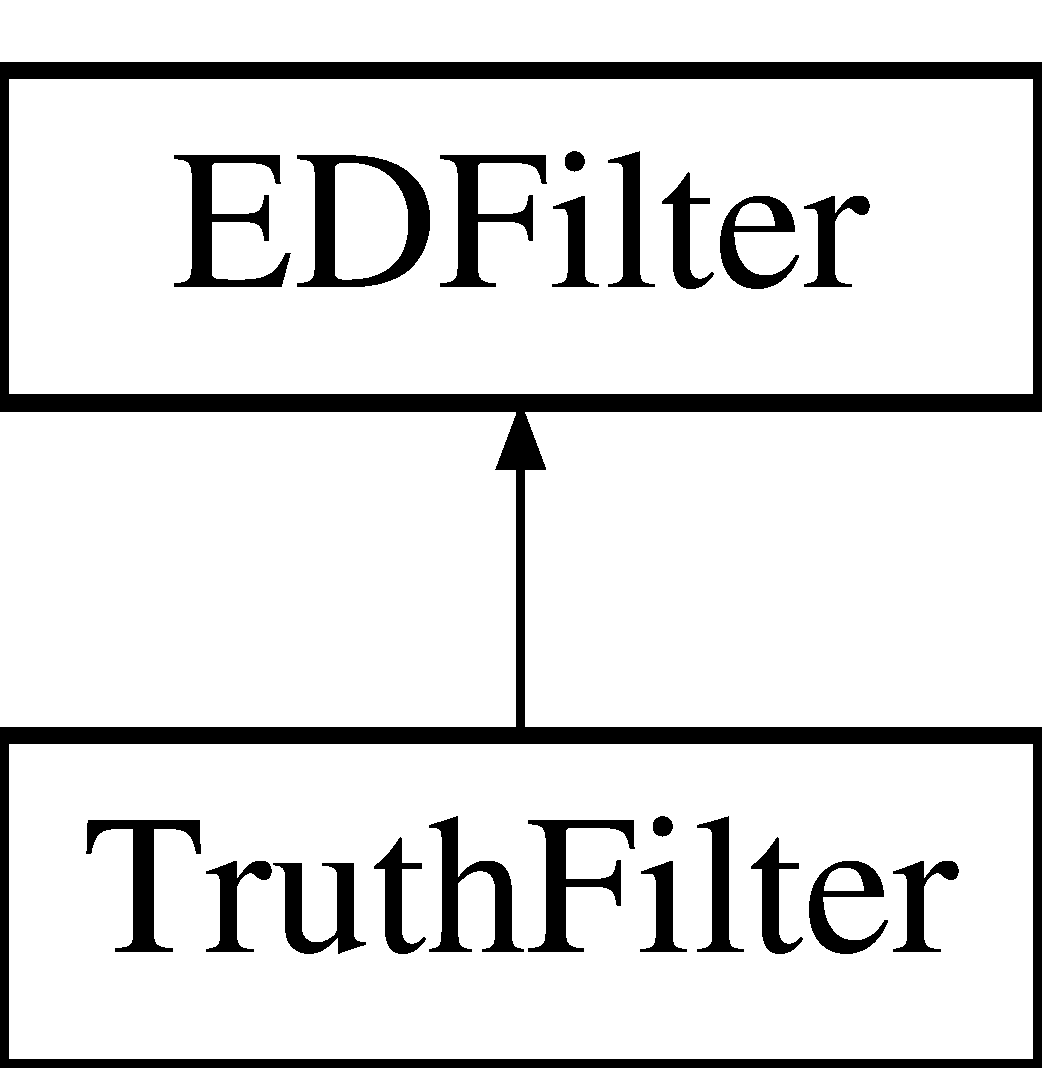
\includegraphics[height=2.000000cm]{classTruthFilter}
\end{center}
\end{figure}
\subsection*{Public Member Functions}
\begin{DoxyCompactItemize}
\item 
\hypertarget{classTruthFilter_ac78d452c321386fa30dd021a1498e6d7}{{\bfseries Truth\-Filter} (fhicl\-::\-Parameter\-Set const \&p)}\label{classTruthFilter_ac78d452c321386fa30dd021a1498e6d7}

\item 
\hypertarget{classTruthFilter_a3bb3577f75d6de9e0bd2cbaf9b51fb3a}{{\bfseries Truth\-Filter} (\hyperlink{classTruthFilter}{Truth\-Filter} const \&)=delete}\label{classTruthFilter_a3bb3577f75d6de9e0bd2cbaf9b51fb3a}

\item 
\hypertarget{classTruthFilter_a634dcfa981c7b34b202a825c7f550ea2}{{\bfseries Truth\-Filter} (\hyperlink{classTruthFilter}{Truth\-Filter} \&\&)=delete}\label{classTruthFilter_a634dcfa981c7b34b202a825c7f550ea2}

\item 
\hypertarget{classTruthFilter_adf7a3c444198d4b2ea0450a29a6ebe8a}{\hyperlink{classTruthFilter}{Truth\-Filter} \& {\bfseries operator=} (\hyperlink{classTruthFilter}{Truth\-Filter} const \&)=delete}\label{classTruthFilter_adf7a3c444198d4b2ea0450a29a6ebe8a}

\item 
\hypertarget{classTruthFilter_a890d5add6632b2be43406dd075ac707e}{\hyperlink{classTruthFilter}{Truth\-Filter} \& {\bfseries operator=} (\hyperlink{classTruthFilter}{Truth\-Filter} \&\&)=delete}\label{classTruthFilter_a890d5add6632b2be43406dd075ac707e}

\item 
\hypertarget{classTruthFilter_a2e4f8564b410b41b253527bec0879a72}{bool {\bfseries filter} (art\-::\-Event \&e) override}\label{classTruthFilter_a2e4f8564b410b41b253527bec0879a72}

\item 
\hypertarget{classTruthFilter_a1ef8e6334b66ae5433e92f4b18a528a1}{void {\bfseries begin\-Job} () override}\label{classTruthFilter_a1ef8e6334b66ae5433e92f4b18a528a1}

\item 
\hypertarget{classTruthFilter_a2f817fb39d4f66f406557ba0aa50727c}{void {\bfseries end\-Job} () override}\label{classTruthFilter_a2f817fb39d4f66f406557ba0aa50727c}

\end{DoxyCompactItemize}
\subsection*{Private Attributes}
\begin{DoxyCompactItemize}
\item 
\hypertarget{classTruthFilter_a17edb6af974475826b0a8b9e18c289e8}{float {\bfseries f\-Enulow}}\label{classTruthFilter_a17edb6af974475826b0a8b9e18c289e8}

\item 
\hypertarget{classTruthFilter_a982d272becaf972f8f39a9735762d58d}{float {\bfseries f\-Enuhigh}}\label{classTruthFilter_a982d272becaf972f8f39a9735762d58d}

\item 
\hypertarget{classTruthFilter_a9dd14e4912aeaea0871aa1683bdfd4b5}{float {\bfseries f\-Proton\-Threshold}}\label{classTruthFilter_a9dd14e4912aeaea0871aa1683bdfd4b5}

\item 
\hypertarget{classTruthFilter_a0dcfc4bfb7d01bf7290bd0cb0d531659}{bool {\bfseries f\-Fiducial\-Volume}}\label{classTruthFilter_a0dcfc4bfb7d01bf7290bd0cb0d531659}

\item 
\hypertarget{classTruthFilter_a69b68c339f5b958a436bb370842f6880}{bool {\bfseries f\-C\-C\-N\-C}}\label{classTruthFilter_a69b68c339f5b958a436bb370842f6880}

\item 
\hypertarget{classTruthFilter_a1896a896e527f01cdaf57d9fd2a70d6f}{bool {\bfseries f\-Neutral\-Current}}\label{classTruthFilter_a1896a896e527f01cdaf57d9fd2a70d6f}

\item 
\hypertarget{classTruthFilter_a9063ad664e9c091c25b719a4e492c965}{bool {\bfseries f\-Charged\-Current}}\label{classTruthFilter_a9063ad664e9c091c25b719a4e492c965}

\item 
\hypertarget{classTruthFilter_a8ae8363120360281655b37ffbce3ac66}{int {\bfseries f\-Npi0}}\label{classTruthFilter_a8ae8363120360281655b37ffbce3ac66}

\end{DoxyCompactItemize}


The documentation for this class was generated from the following file\-:\begin{DoxyCompactItemize}
\item 
/home/travis/build/ubneutrinos/searchingfornues/\-Filters/Truth\-Filter\-\_\-module.\-cc\end{DoxyCompactItemize}

%--- End generated contents ---

% Index
\newpage
\phantomsection
\addcontentsline{toc}{chapter}{Index}
\printindex

\end{document}
